\RequirePackage{ifthen}
\newboolean{longpage}
\setboolean{longpage}{false}
\ifthenelse{\boolean{longpage}}%
{\documentclass[10pt]{article}}%
{\documentclass[10pt]{book}}

\newboolean{printlabelname}
\setboolean{printlabelname}{false}
\ifthenelse{\boolean{printlabelname}}{\usepackage[notref,notcite]{showkeys}}{}

\usepackage{refcount}
\usepackage{pdfpages}

\newboolean{colour}
\setboolean{colour}{true}
\newboolean{CalcIII}
\setboolean{CalcIII}{false}
\newboolean{CalcIV}
\setboolean{CalcIV}{true}


%% end detour
%\usepackage{amsmath}
\usepackage{xr}
\externaldocument[I-]{Math1560_ebook}\externaldocument[II-]{Math2560_ebook}
\externaldocument[III-]{Math2570_ebook}

%%Page Size stuff

\newboolean{tabletsize}
\ifthenelse{\boolean{longpage}}% if longpage, tablet automatically false
{\setboolean{tabletsize}{false}}%% if not longpage, then set tablet
{\setboolean{tabletsize}{false}}

%% Layout for printed book through Amazon CreateSpace, perfect bound,
%% 8.5 x 11 paper size, 1in inner margin, 1/2in (roughly) outer margin

%% for regular sized pages
\ifthenelse{\boolean{longpage}}%
				{\usepackage[paperheight=20in,
				paperwidth=7in,%inner=1in,
				textheight=18in,textwidth=320pt%,marginparwidth=150pt,marginparsep=32pt
				]{geometry}}%
				%% else not long page; 
				{% not longpage
				\usepackage[paperheight=11in,paperwidth=8.5in,%
						inner=1in,textheight=9in,textwidth=320pt,marginparwidth=150pt,%
						marginparsep=32pt,bottom=1in,footskip=29pt]{geometry}}

\ifthenelse{\boolean{longpage}}%
{% longpage - do not make changes to the text height for exercises
\newcommand{\exercisegeometry}{%
\newgeometry{inner=72pt,outer=72pt,textheight=18in,%textwidth=320pt,
						marginparwidth=150pt,marginparsep=32pt}
															}
}% ends if longpage
{% not longpage - regular sized exercise sets
%%
%% the old size of exercises
%
%\newcommand{\exercisegeometry}{%
%\newgeometry{inner=72pt,%
						%outer=72pt,textheight=545pt,%textwidth=320pt,
						%marginparwidth=150pt,%
						%marginparsep=32pt,
						%}
															%}
%%
%% the new size of exercises
%%
\newcommand{\exercisegeometry}{%
\newgeometry{inner=72pt,%
						outer=72pt,textheight=9.25in,tmargin=.75in,%textwidth=320pt,
						marginparwidth=150pt,%
						marginparsep=32pt,footskip=29pt,
						%bottom=1in,
						}
															}
}% ends if/then/else longpage

\newcommand{\eendgeometry}{%
\newgeometry{inner=72pt,%
						outer=36pt,textheight=10in,%textwidth=320pt,
						marginparwidth=150pt,%
						marginparsep=32pt,
						%bottom=1in%,footskip=1.5in
						}%
													}

\newcommand{\prefacegeometry}{%
\newgeometry{inner=1in,textheight=9in,textwidth=320pt,marginparwidth=150pt,%
						marginparsep=32pt,bottom=1in,footskip=1.5in}
															}


\ifthenelse{\boolean{longpage}}{%
	\usepackage{everyshi}
	\textheight500cm
	\EveryShipout{%
	\pdfpagewidth=7in
	\pdfpageheight=\pagetotal
	\advance\pdfpageheight by 3in
	\advance\pdfpageheight by 2\topmargin
	\advance\pdfpageheight by \textheight
	\advance\pdfpageheight by -\pagegoal}
%%
	\newcounter{chapter}
	\newcommand{\chapter}{\refstepcounter{chapter}\Huge Chapter \thechapter \vskip 2\baselineskip\normalsize}
}{}


\usepackage{APEX_format}
%%%%
% Additional packages to support the book, not part of the APEX style.
%%%%
\usepackage{fancyhdr}
\usepackage{eso-pic}
\usepackage{lipsum}
\usepackage{units}
%\usepackage{pgfplots}
%\pgfplotsset{width=\marginparwidth+1pt,compat=1.3}
\usepackage[font=small]{caption}
%,justification=centering

%%%%
%% These are low level LaTeX commands that determine the 
%% look of the Chapter and Section headings.
%% Note the use in the chapter part of an external file
%% that contains graphics for each chapter start.
%%%%

%%%%
%% Commands for the header, utilizing the fancyhdr
%% (fancy header) package
%%%%

\pagestyle{fancy}
\fancyhead{}
%\fancyfoot{}
\renewcommand{\chaptermark}[1]{\markboth{\chaptername\ \thechapter\ \ \ \ {#1}}{}}
\renewcommand{\sectionmark}[1]{\markright{\thesection\ \ \ \  #1}}
\fancyhf{}         %Clears all header and footer fields, in preparation.
\renewcommand{\headrulewidth}{0pt}
\renewcommand{\footrulewidth}{0pt}

\ifthenelse{\boolean{longpage}}%
{}% end header of longpage
{% begin header/footer of not longpage
\fancyhfoffset[LE,RO]{\marginparwidth+\marginparsep}
%\fancyfoot[LE,RO]{\textbf{\thepage}} %Displays the page number in bold in the header,

\fancyfoot{}
\fancyfoot[LE]{\textbf{\thepage}}
\fancyfoot[RO]{\textbf{\thepage}}

%\fancyfoot[LE]{\begin{minipage}{\textwidth}%
%\noindent\hskip\marginparwidth\hskip\marginparsep\hskip-4pt\rule{\textwidth}{.4pt}
%\vskip.2\baselineskip
%\noindent\hskip\marginparwidth\hskip\marginparsep\hskip-4pt%
%Notes:
%\vskip 1.5in\textbf{\thepage}
%\end{minipage}} 

%\fancyfoot[RO]{\begin{minipage}{\textwidth+\marginparwidth+\marginparsep}%
%\rule{\textwidth-\marginparwidth-\marginparsep}{.4pt}
%\vskip.2\baselineskip
%Notes:
%\vskip 1.5in
%\hfill\textbf{\thepage}
%\end{minipage}}       


\fancyhead[LE]{\nouppercase{\leftmark}}
      %Displays the upper-level (chapter) information---
      % as determined above---in non-upper case in the header, 
      %to the right on even pages.
\fancyhead[RO]{\rightmark}
			%Displays the lower-level (section) information---as
      % determined above---in the header, to the left on odd pages.
      
}% End the ifthenelse{longpage}


\ifthenelse{\boolean{longpage}}% for changing the header
{% longpage
\newcommand{\exerciseheader}{}
\newcommand{\regularheader}{}
\newcommand{\endmatheader}{}
}% i.e, the above does nothing
{% now for a real change
\newcommand{\exerciseheader}{%
				\fancyhfoffset[LE,RO]{32pt}%
				\fancyfoot[LE]{\textbf{\thepage}}% 
				\fancyfoot[RO]{\textbf{\thepage}}
				\fancyhead{}% 
}

\newcommand{\regularheader}{%
\fancyhead[LE]{\nouppercase{\leftmark}}%
\fancyhead[RO]{\rightmark}%
%\fancyfoot[LE]{}
%\fancyfoot[RO]{}
\fancyfoot{}
\fancyfoot[LE]{\textbf{\thepage}}
\fancyfoot[RO]{\textbf{\thepage}}
%\fancyfoot[LE]{\begin{minipage}{\textwidth}%
%\noindent\hskip\marginparwidth\hskip\marginparsep\hskip-4pt\rule{\textwidth}{.4pt}
%\vskip.2\baselineskip
%\noindent\hskip\marginparwidth\hskip\marginparsep\hskip-4pt%
%Notes:
%\vskip 1.5in\textbf{\thepage}
%\end{minipage}} 

%\fancyfoot[RO]{\begin{minipage}{\textwidth+\marginparwidth+\marginparsep}%
%\rule{\textwidth-\marginparwidth-\marginparsep}{.4pt}
%\vskip.2\baselineskip
%Notes:
%\vskip 1.5in
%\hfill\textbf{\thepage}
%\end{minipage}}

\fancyhfoffset[LE,RO]{\marginparsep+\marginparwidth}
}

\newcommand{\qendheader}{%
		\fancyhead{}%
		\fancyfoot{}%
		}
}% ends if/then/else exercise/regular headers


%
%  Defining what the chapter titles look like
%

\newdimen\titleheight

\makeatletter
\def\@makechapterhead#1{%
  {\parindent \z@ \raggedright \reset@font
    {\Huge \thechapter: \scshape \textsc #1}
    \par\vskip 10\p@
    \hrule height 1pt
    \vskip 10\p@
  }}
%%  
%%%\makeatletter
%%\def\@makesectionhead#1{%
%%	 {\reset@font\LARGE\itshape\bfseries\strut #1 \thechapter.\thesection \ #1
%%	 }}

%%%%
%%
%%  For figures in the margin
%%
%%%%

%%\usepackage{wrapfig}
%%
%%\setlength{\marginparsep}{10pt}
%%\setlength{\wrapoverhang}{\marginparwidth}
%%\addtolength{\wrapoverhang}{\marginparsep}
%%
%%%\newenvironment{mfigure}[1]{%
%%%    \wrapfigure{#1}{0pt}%
%%%    \begin{minipage}{\marginparwidth}%
%%%    \centering%
%%%}{%
%%%    \end{minipage}%
%%%    \endwrapfigure%
%%%}


\ifthenelse{\boolean{longpage}}%
		{\newcommand{\mfigure}[5][]{%
		\vskip \baselineskip%
			\noindent\begin{minipage}{\textwidth}
  			\centering
  			\myincludegraphics{#5}
  			#1%
  			\captionsetup{type=figure}
	  		\caption{#3}\label{#4}
  		\end{minipage}
		}}
		{\newcommand{\mfigure}[5][]{%
		\ifthenelse{\isodd{\thepage}}%
			{\AddToShipoutPicture*{\put(427,\LenToUnit{#2\paperheight}){%
			\begin{minipage}{\marginparwidth}%
				\centering%
	  		\myincludegraphics[#1]{#5}%
  			\captionsetup{type=figure}%
  			%#1%
	  		\caption{#3}\label{#4}%
  		\end{minipage}}}}%
			{\AddToShipoutPicture*{\put(36,\LenToUnit{#2\paperheight}){%
			\begin{minipage}{\marginparwidth}%
			  \centering%
  			\myincludegraphics[#1]{#5}%
  			\captionsetup{type=figure}%
  			%#1%
	  		\caption{#3}\label{#4}%
  		\end{minipage}}}}%
		}}%

\ifthenelse{\boolean{longpage}}%
		{\newcommand{\mtable}[4]{
					\vskip \baselineskip%
					\noindent\begin{minipage}{\textwidth}
  					\centering\small
  					#4
  					\captionsetup{type=figure}
	  				\caption{#2}\label{#3}
  				\end{minipage}
  				\vskip\baselineskip}
  	}
		{\newcommand{\mtable}[4]{%
			\ifthenelse{\isodd{\thepage}}%
				{\AddToShipoutPicture*{\put(427,\LenToUnit{#1\paperheight}){%
					\begin{minipage}{\marginparwidth}%
  					\centering\small%
  					#4%
  					\captionsetup{type=figure}%
	  				\caption{#2}\label{#3}%
  				\end{minipage}}}}%
				{\AddToShipoutPicture*{\put(36,\LenToUnit{#1\paperheight}){%
					\begin{minipage}{\marginparwidth}%
 						 \centering\small%
 						 #4%
						  \captionsetup{type=figure}%
	  					\caption{#2}\label{#3}%
 					 \end{minipage}}}}%
		}}%

\ifthenelse{\boolean{longpage}}%
		{\newcommand{\mnote}[2]{%
					\hskip 25pt%
					\begin{minipage}{\marginparwidth}%
					\small%
					#2%
					\end{minipage}%
					\vskip\baselineskip%
		}%
		}%
		{\newcommand{\mnote}[2]{%
			\ifthenelse{\isodd{\thepage}}%
				{\AddToShipoutPicture*{\put(427,\LenToUnit{#1\paperheight}){%
					\begin{minipage}{\marginparwidth}
  					\small
  					#2
  				\end{minipage}}}}%
				{\AddToShipoutPicture*{\put(36,\LenToUnit{#1\paperheight}){%
					\begin{minipage}{\marginparwidth}
 						 \small
 						 #2
					\end{minipage}}}}
		}}

%\ifthenelse{\boolean{longpage}}%
		%{}
		%{\newcommand{\mfigurethree}[5][]{%
		%\ifthenelse{\isodd{\thepage}}%
			%{\AddToShipoutPicture*{\put(427,\LenToUnit{#2\paperheight}){%
			%\begin{minipage}{\marginparwidth}%
				%\centering%
	  		%\includemedia[#1]{\includegraphics{#5}}{#5.prc}%
  			%\captionsetup{type=figure}%
  			%%#1%
	  		%\caption{#3}\label{#4}%
  		%\end{minipage}}}}%
			%{\AddToShipoutPicture*{\put(36,\LenToUnit{#2\paperheight}){%
			%\begin{minipage}{\marginparwidth}%
			  %\centering%
  			%\includemedia[#1]{\includegraphics{#5}}{#5.prc}%
  			%\captionsetup{type=figure}%
  			%%#1%
	  		%\caption{#3}\label{#4}%
  		%\end{minipage}}}}%
		%}}%
		
		\newcommand{\mfigurethree}[6]{%
		\ifthenelse{\isodd{\thepage}}%
			{\AddToShipoutPicture*{\put(427,\LenToUnit{#3\paperheight}){%
			\begin{minipage}{\marginparwidth}%
				\centering%
				\ifthenelse{\boolean{in_threeD}}{% in 3D
	  		\includemedia[#1]{\includegraphics{#6_3D\colornamesuffix}}{#6_3D.prc}}%now not in 3D
				{\myincludegraphics[#2]{#6}}%
  			\captionsetup{type=figure}%
  			%#1%
	  		\caption{#4}\label{#5}%
  		\end{minipage}}}}%
			{\AddToShipoutPicture*{\put(36,\LenToUnit{#3\paperheight}){%
			\begin{minipage}{\marginparwidth}%
			  \centering%
  			\ifthenelse{\boolean{in_threeD}}{% in 3D
	  		\includemedia[#1]{\includegraphics{#6_3D\colornamesuffix}}{#6_3D.prc}}%now not in 3D
				{\myincludegraphics[#2]{#6}}%
  			\captionsetup{type=figure}%
  			%#1%
	  		\caption{#4}\label{#5}%
  		\end{minipage}}}}%
		}

%\AddToShipoutPicture{\ifthenelse{\ifodd{\thepage}}%
%{\put(10,10){\begin{tikzpicture}\draw (0,0) circle (5pt);\end{tikzpicture}}}%
%{\put(100,100){\begin{tikzpicture}\draw (0,0) circle (5pt);\end{tikzpicture}}}}%
%

%\AddToShipoutPictureBG{%
% \AtPageLowerLeft{\hspace{1cm}A small logo: \rule{2cm}{3cm}}}
% 
%}{\AddToShipoutPicture*{\put(36,\LenToUnit{#2\paperheight})}}%
%{%
%\begin{minipage}{\marginparwidth}
%  \centering
%  \includegraphics{#1}
%  \captionof{figure}{#3}
%  \end{minipage}}}
%\AddToShipoutPicture*{\put(\LenToUnit{.5\paperwidth},\LenToUnit{.75\paperheight}){%
%  \begin{minipage}{100pt}
%  \centering
%  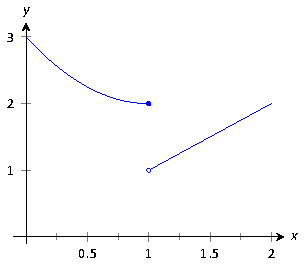
\includegraphics{test-figure2.pdf}
%  \captionof{figure}{Test caption}
%  \end{minipage}}}


%\newenvironment{mfigurefile}[2]{%
%\begin{tikzpicture}[remember picture,overlay]%
%\ifthenelse{\isodd{\thepage}}{\node [xshift=-36pt-.5\marginparwidth,yshift=#2\paperheight] at (current page.south east) }{\node [xshift=36pt+.5\marginparwidth,yshift=#2\paperheight] at (current page.south west) }%
%{\input{#1}};}%
%{\end{tikzpicture}%
%}

%\DeclareCaptionType{mytype}[Typename][List of mytype]


    
%%%%
%% End margin figure 
%%%%    
    

\newcommand{\bmx}[1]{\left[\hskip -3pt\begin{array}{#1} }
\newcommand{\emx}{\end{array}\hskip -3pt\right]}

\newcommand{\btz}{\begin{center}\begin{tikzpicture}}
\newcommand{\etz}{\end{tikzpicture}\end{center}}

\newcommand{\ds}{\displaystyle}

\newcommand{\fp}{\ensuremath{f\,'}}
\newcommand{\fpp}{\ensuremath{f\,''}}

\newcommand{\Fp}{\ensuremath{F\primeskip'}}
\newcommand{\Fpp}{\ensuremath{F\primeskip''}}

\newcommand{\yp}{\ensuremath{y\primeskip'}}
\newcommand{\gp}{\ensuremath{g\primeskip'}}

\newcommand{\dx}{\ensuremath{\Delta x}}
\newcommand{\dy}{\ensuremath{\Delta y}}
%\newcommand{\dz}{\ensuremath{\Delta z}}
\newcommand{\ddz}{\ensuremath{\Delta z}}

\newcommand{\thet}{\ensuremath{\theta}}
\newcommand{\norm}[1]{\ensuremath{||\ #1\ ||}}
\newcommand{\vnorm}[1]{\ensuremath{\norm{\vec #1}}}
\newcommand{\snorm}[1]{\ensuremath{\left|\left|\ #1\ \right|\right|}}
\newcommand{\la}{\left\langle}
\newcommand{\ra}{\right\rangle}
\newcommand{\dotp}[2]{\ensuremath{\vec #1 \cdot \vec #2}}
\newcommand{\proj}[2]{\ensuremath{\text{proj}_{\,\vec #2}{\,\vec #1}}}
\newcommand{\crossp}[2]{\ensuremath{\vec #1 \times \vec #2}}
\newcommand{\veci}{\ensuremath{\vec i}}
\newcommand{\vecj}{\ensuremath{\vec j}}
\newcommand{\veck}{\ensuremath{\vec k}}
\newcommand{\vecu}{\ensuremath{\vec u}}
\newcommand{\vecv}{\ensuremath{\vec v}}
\newcommand{\vecw}{\ensuremath{\vec w}}
\newcommand{\vecx}{\ensuremath{\vec x}}
\newcommand{\vecy}{\ensuremath{\vec y}}
\newcommand{\vrp}{\ensuremath{\vec r\, '}}
\newcommand{\vsp}{\ensuremath{\vec s\, '}}
\newcommand{\vrt}{\ensuremath{\vec r(t)}}
\newcommand{\vst}{\ensuremath{\vec s(t)}}
\newcommand{\vvt}{\ensuremath{\vec v(t)}}
\newcommand{\vat}{\ensuremath{\vec a(t)}}
\newcommand{\px}{\ensuremath{\partial x}}
\newcommand{\py}{\ensuremath{\partial y}}
\newcommand{\pz}{\ensuremath{\partial z}}
\newcommand{\pf}{\ensuremath{\partial f}}
\newcommand{\underlinespace}{\underline{\phantom{xxxxxx}}}

\newcommand{\mathN}{\ensuremath{\mathbb{N}}}

\newcommand{\zerooverzero}{\ensuremath{\ds \raisebox{8pt}{\text{``\ }}\frac{0}{0}\raisebox{8pt}{\text{\ ''}}}}


\newcommand{\myrule}{\rule[-4pt]{0pt}{13pt}}
\newcommand{\mmrule}{\rule[-10pt]{0pt}{15pt}}
\newcommand{\myds}{\ds\mmrule}
\newcommand{\deriv}[2]{\ensuremath{\myds\frac{d}{dx}\left(#1\right)=#2}}
\newcommand{\myint}[2]{\ensuremath{\myds\int #1\ dx=} \ensuremath{\ds #2}}

\DeclareMathOperator{\sech}{sech}
\DeclareMathOperator{\csch}{csch}

\newcommand{\sword}[1]{\textbf{#1}}

\newcommand{\primeskip}{\hskip.75pt}

%%%% Begin Header TikZ

%  Some TiKZ  shortcuts to help make drawing 3D vectors faster.
%

\newcommand{\plotlinecolor}{blue}

%
% Draw x and y tick marks
%
\newcommand{\drawxticks}[1]
{\foreach \x in {#1}
		{\draw  (\x,-.1)--(\x,.1);
			};
}
\newcommand{\drawyticks}[1]
{\foreach \x in {#1}
		{\draw  (-.1,\x)--(.1,\x);
			};
}

\newcommand{\drawxlines}[3]
{\draw[<->] (#1,0) -- (#2,0) node [right] {$x$};
\foreach \x in {#3}
		{\draw  (\x,-.1)--(\x,.1);
			};
}

\newcommand{\drawylines}[3]
{\draw[<->] (0,#1) -- (0,#2) node [above] {$y$};
\foreach \x in {#3}
		{\draw  (-.1,\x)--(.1,\x);
			};
}

\newcommand{\drawxlabels}[1]
{\foreach \x in {#1}
		{\draw  (\x,-.1) node [below] {\scriptsize $\x$};
		};
}

\newcommand{\drawylabels}[1]
{\foreach \x in {#1}
		{\draw  (-.1,\x) node [left] {\scriptsize $\x$};
		};
}

%% draw a box of margin width size to see if figure is properly contained within
\newcommand{\marginsizebox}{\draw (0,0)--(\marginparwidth,0)--(\marginparwidth,3)--(0,3)--cycle;}

%%%%
%%%%

\newcommand{\asyouread}[1]{\begin{tikzpicture}
\ifthenelse{\boolean{in_color}}{\node [preaction={fill=black,opacity=.5,transform canvas={xshift=1mm,yshift=-1mm}}, right color=blue!80!black!30, left color=blue!80] at (0,0) {\textcolor{white}{\textsf{\textit{AS YOU READ $\ldots$}}}};}
{\node [preaction={fill=black,opacity=.5,transform canvas={xshift=1mm,yshift=-1mm}}, right color=black!30, left color=black!10] at (0,0) {\textcolor{white}{\textsf{\textit{AS YOU READ $\ldots$}}}};}
\end{tikzpicture}
\begin{enumerate}
#1
\end{enumerate}
\vskip 20pt}

%%%%
%%  A new figure environment, trying to fix the float problem.
%%
%%%%

\newcounter{myfigurecounter}[chapter]
\renewcommand\themyfigurecounter{\thechapter.\arabic{myfigurecounter}}
\newenvironment{myfigure}{\refstepcounter{myfigurecounter}}{}
\newcommand{\mycaption}[1]{%
\begin{center}%
\vskip -1.5\baselineskip
\begin{tikzpicture}%
\draw (0,0) node [text width=\textwidth,align=center] {Figure \themyfigurecounter: #1};%
\end{tikzpicture}%
\end{center}%
}
\usepackage{pgfplots}
\pgfplotsset{compat=1.8}


\ifthenelse{\boolean{xetex}}%
	{\sffamily
	%%\usepackage{fontspec}
	\usepackage{mathspec}
	\setallmainfonts[Mapping=tex-text]{Calibri}
	\setmainfont[Mapping=tex-text,Ligatures=NoCommon]{Calibri}
	\setsansfont[Mapping=tex-text,Ligatures=NoCommon]{Calibri}
	\setmathsfont(Greek){[cmmi10]}}
	{\usepackage[sfdefault,lf]{carlito}
%% The 'lf' option for lining figures
%% The 'sfdefault' option to make the base font sans serif
\usepackage[T1]{fontenc}
\renewcommand*\oldstylenums[1]{\carlitoOsF #1}}
	
	\ifthenelse{\boolean{luatex}}%
	{\sffamily
	\usepackage{fontspec}
	\usepackage{unicode-math}
	%\usepackage{mathspec}
	%\setallmainfonts[Mapping=tex-text]{Calibri}
	\setmainfont{Calibri}
	%\setsansfont[Mapping=tex-text]{Calibri}
	\setmathfont[range=\mathup]{Calibri}
	\setmathfont[range=\mathit]{Calibri Italic}
	}
	{}

\makeindex

%%%\tracingonline=1
\begin{document}


\ifthenelse{\boolean{colour}}{\printincolor}{\printinblackandwhite}

%\printexercisenames
%\printallanswers

%
%%%%%%%%%%
%%%
%%%  Set criteria for the format of the book.
%%%  This supercedes anything set in the Text_Header.
%%%
%%%%%%%%%%



%\printinblackandwhite

%\printexercisenames

%\nodrawexamplelines

%\printallanswers


\normalem



%%%\pagenumbering{roman}

%%%%%%
%%%		For editing purposes, block comment down to 
%%%		the next mark
%%%%%%

%%%%\input{cover/front_cover_in_text}
%%%%\clearpage
%%%%\thispagestyle{empty}
\frontmatter
%%%%
%%%%\title{\textsc{Fundamentals of Matrix Algebra}\\
%%%%{\small Version 2.1011}}
%%%%\author{Gregory N. Hartman, Ph.D.}
%%%%\date{}

\vspace*{\stretch{.5}}

\hskip 125pt\begin{minipage}{\textwidth}
\begin{flushright}

\textsc{{\Huge Math 2580 Calculus IV}} \\

\textsl{\large Fall 2018 Edition}, 
{\large University of Lethbridge}\\

{An adaptation of the \apex\ Calculus textbook, edited by Sean Fitzpatrick}

\bigskip

\Large
%\vspace{1in}

Gregory Hartman, Ph.D.

\emph{\small Department of Applied Mathematics}

\emph{\small Virginia Military Institute}\vskip15pt

%Ji{\v r}\'i Lebl, Ph.D.

%\emph{\small Department of Mathematics}

%\emph{\small University of Oklahoma}

\parbox{200pt}{\textit{Contributing Authors}}\hskip 2cm \phantom{.}

Troy Siemers, Ph.D.

\emph{\small Department of Applied Mathematics}

\emph{\small Virginia Military Institute}\vskip 15pt

Brian Heinold, Ph.D.

\emph{\small Department of Mathematics and Computer Science}

\emph{\small Mount Saint Mary's University}\vskip 15pt

Dimplekumar Chalishajar, Ph.D.

\emph{\small Department of Applied Mathematics}

\emph{\small Virginia Military Institute}\vskip 25pt



\parbox{200pt}{\textit{Editor}}\hskip 2cm \phantom{.}
%\textit{Editor}\hskip 7cm\phantom{.}

Jennifer Bowen, Ph.D.

\emph{\small Department of Mathematics and Computer Science}

\emph{\small The College of Wooster}


\normalsize
\end{flushright}
\end{minipage}

\vspace{\stretch{1}}


\thispagestyle{empty}
\clearpage

\vspace*{\stretch{5}}
\noindent\hskip -1in\begin{minipage}{2in}
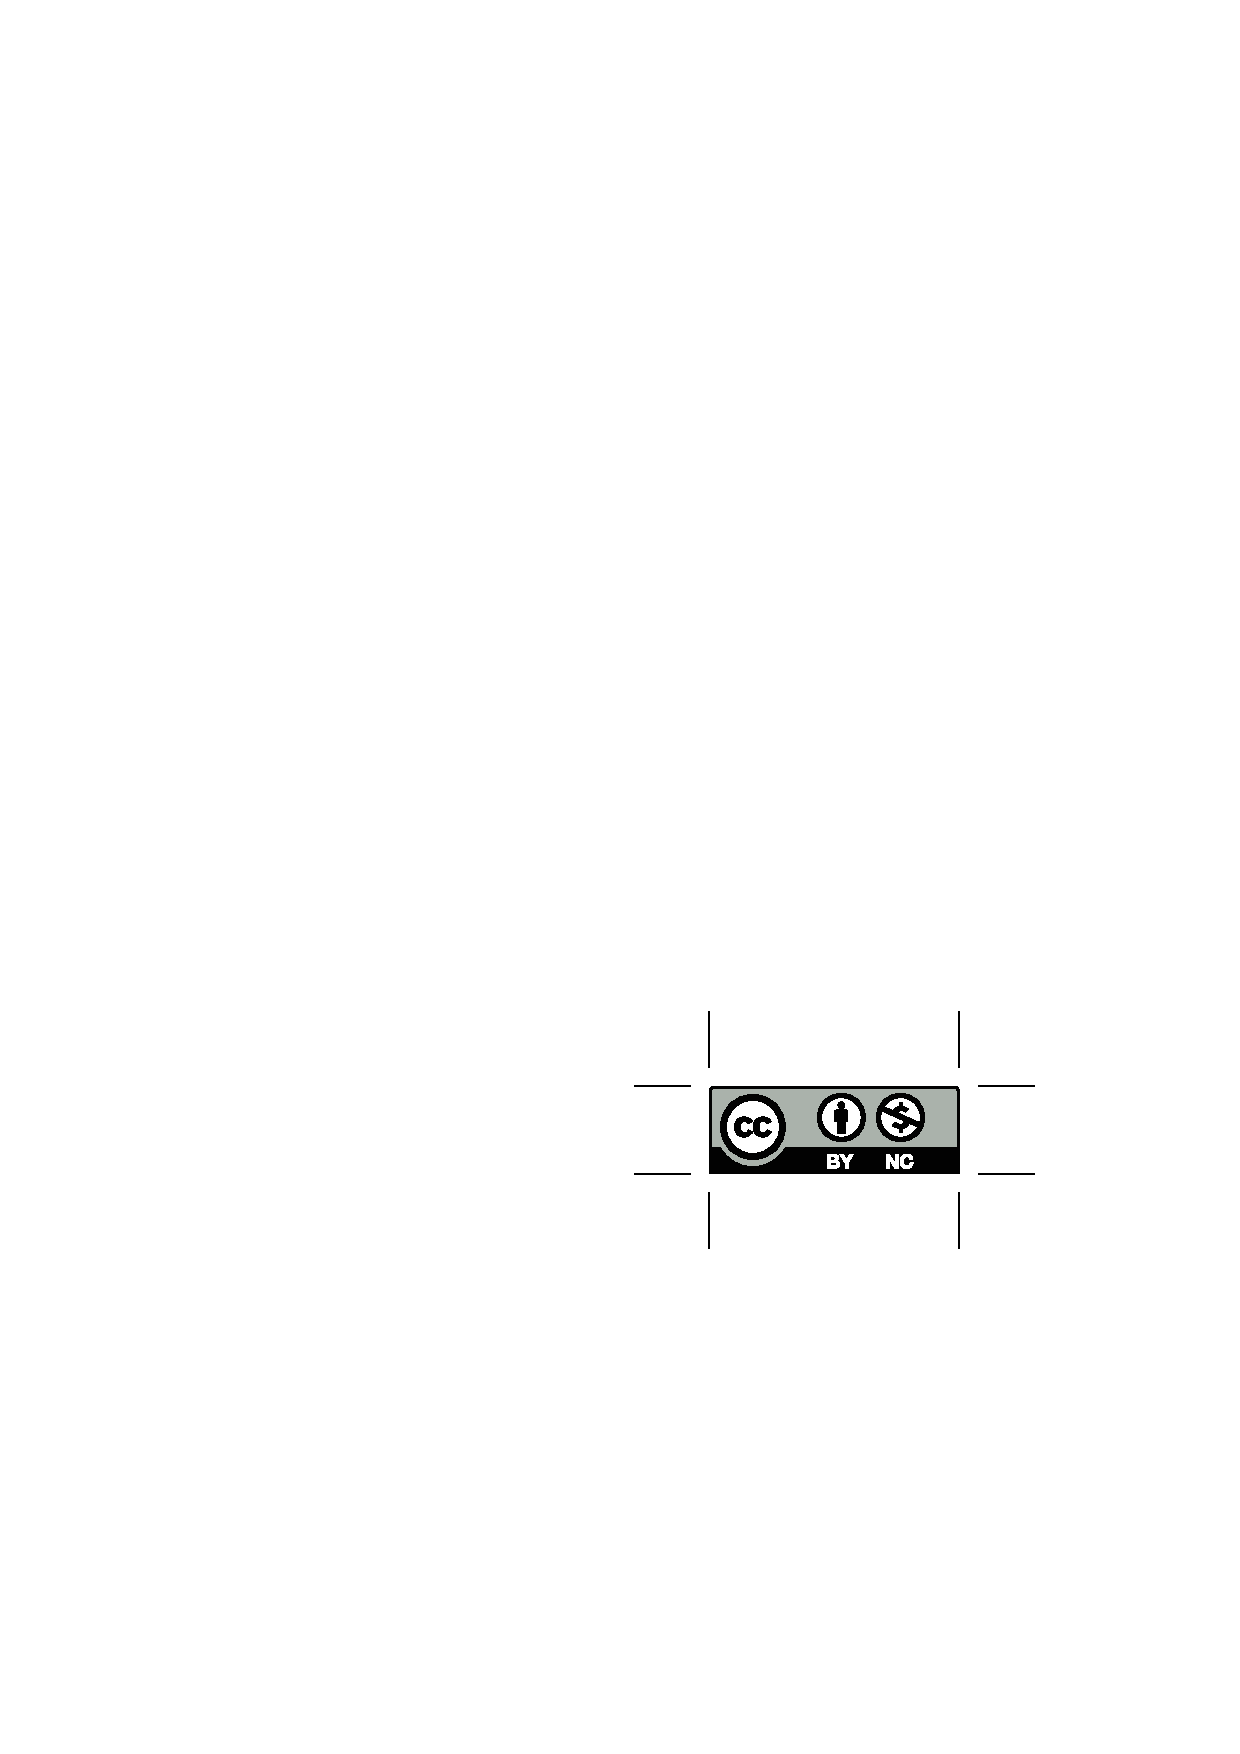
\includegraphics{text/by-nc} 
\end{minipage}
\begin{minipage}{3in}
\noindent Copyright \copyright\ 2018 Gregory Hartman

Licensed to the public under Creative Commons Attribution-Noncommercial 4.0 International Public License
\end{minipage}

\bigskip

\bigskip



\bigskip

\begin{minipage}{3.3in}
This version of the text was assembled and edited by Sean Fitzpatrick, University of Lethbridge, in May 2018. 

This work is licensed under the Creative Commons Attribution-Noncommercial-ShareAlike 4.0 International Public License
\end{minipage}
\vspace{\stretch{1}} 
\thispagestyle{empty}
\clearpage


%\cleardoublepage
%%%%\phantomsection
%%%%\input{text/thanks}
\addtocontents{toc}{\protect\thispagestyle{empty}}
%%%%\addcontentsline{toc}{chapter}{Thanks} 
%%%%\clearpage{\pagestyle{empty}\cleardoublepage}
%%%%\phantomsection
%%%%\thispagestyle{empty}
\Huge
\noindent {\bf \textsc{Preface}}\\
\large
\emph{A Note on Using this Text}
\vspace{1in}
\normalsize

Thank you for reading this short preface. Allow us to share a few key points about the text so that you may better understand what you will find beyond this page.

This text comprises a three--volume series on Calculus. The first part covers material taught in many ``Calc 1'' courses: limits, derivatives, and the basics of integration, found in Chapters 1 through 6.1. The second text covers material often taught in ``Calc 2:'' integration and its applications, along with an introduction to sequences, series and Taylor Polynomials, found in Chapters 5 through 8. The third text covers topics common in ``Calc 3'' or ``multivariable calc:'' parametric equations, polar coordinates, vector--valued functions, and functions of more than one variable, found in Chapters 9 through 13. All three are available separately for free at \texttt{\href{http://apexcalculus.com}{www.apexcalculus.com}}. %These three texts are intended to work together and make one cohesive text, \textit{APEX Calculus}, which can also be downloaded from the website. 

Printing the entire text as one volume makes for a large, heavy, cumbersome book. One can certainly only print the pages they currently need, but some prefer to have a nice, bound copy of the text. Therefore this text has been split into these three manageable parts, each of which can be purchased for under \$15 at \href{http://amazon.com}{Amazon.com}.\\ 



%A result of this splitting is that sometimes a concept is said to be explored in a ``later section,'' though that section does not actually appear in this particular text. Downloading the .pdf of \textit{APEX Calculus} will ensure that you have all the content.  
%material is referenced that is not contained in the present text. The context should make it clear whether the ``missing'' material is in the \textit{Calculus I} or \textit{Calculus III} portion. Downloading the appropriate .pdf, or the whole \textit{APEX Calculus} .pdf, will give access to these topics.
% This splitting of the material also results in unfortunate page/chapter numberings. Chapter 5 of this text is Chapter 1 of \textit{Calculus II}. Apart from these numberings, page--for--page the content of the sections that appear in both \textit{Calculus I} and \textit{Calculus II} are identical.\\ %For instance, in this text, ``Theorem 20'' may be mentioned, although Theorem 20 is only presented in Part I. To minimize confusion, theorems, definitions and key ideas are referenced by their title or subject matter, not their number.

%The current publisher of this text does not allow one text to be split across multiple volumes, with continuity of chapters and page numberings. This is the one drawback of the current publishing model that has many advantages, highlighted below. Because of this, there are a few peculiarities 

\noindent\textbf{\large For Students: How to Read this Text}\\

Mathematics textbooks have a reputation for being hard to read. High--level mathematical writing often seeks to say much with few words, and this style often seeps into texts of lower--level topics. This book was written with the goal of being easier to read than many other calculus textbooks, without becoming too verbose. 

Each chapter and section starts with an introduction of the coming material, hopefully setting the stage for ``why you should care,'' and ends with a look ahead to see how the just--learned material helps address future problems. 

\textit{Please read the text;} it is written to explain the concepts of Calculus. There are numerous examples to demonstrate the meaning of definitions, the truth of theorems, and the application of mathematical techniques. When you encounter a sentence you don't understand, read it again. If it still doesn't make sense, read on anyway, as sometimes confusing sentences are explained by later sentences.

\textit{You don't have to read every equation.} The examples generally show ``all'' the steps needed to solve a problem. Sometimes reading through each step is helpful; sometimes it is confusing. When the steps are illustrating a new technique, one probably should follow each step closely to learn the new technique. When the steps are showing the mathematics needed to find a number to be used later, one can usually skip ahead and see how that number is being used, instead of getting bogged down in reading how the number was found.

\textit{Most proofs have been omitted.} In mathematics, \textit{proving} something is always true is extremely important, and entails much more than testing to see if it works twice. However, students often are confused by the details of a proof, or become concerned that they should have been able to construct this proof on their own. To alleviate this potential problem, we do not include the proofs to most theorems in the text. The interested reader is highly encouraged to find proofs online or from their instructor. In most cases, one is very capable of understanding what a theorem \textit{means} and \textit{how to apply it} without knowing fully \textit{why} it is true.
\\

\thispagestyle{empty}
\noindent\textbf{\large Interactive, 3D Graphics}\\

New to Version 3.0 is the addition of interactive, 3D graphics in the .pdf version. Nearly all graphs of objects in space can be rotated, shifted, and zoomed in/out so the reader can better understand the object illustrated. 

As of this writing, the only pdf viewers that support these 3D graphics are Adobe Reader \& Acrobat (and only the versions for PC/Mac/Unix/Linux computers, not tablets or smartphones). To activate the interactive mode, click on the image. Once activated, one can click/drag to rotate the object and use the scroll wheel on a mouse to zoom in/out. (A great way to investigate an image is to first zoom in on the page of the pdf viewer so the graphic itself takes up much of the screen, then zoom inside the graphic itself.) A CTRL-click/drag pans the object left/right or up/down. By right-clicking on the graph one can access a menu of other options, such as changing the lighting scheme or perspective. One can also revert the graph back to its default view. If you wish to deactive the interactivity, one can right-click and choose the ``Disable Content'' option. \\

\noindent\textbf{\large Thanks}\\

There are many people who deserve recognition for the important role they have played in the development of this text. First, I thank Michelle for her support and encouragement, even as this ``project from work'' occupied my time and attention at home. Many thanks to Troy Siemers, whose most important contributions extend far beyond the sections he wrote or the 227 figures he coded in Asymptote for 3D interaction.  He provided incredible support, advice and encouragement for which I am very grateful. My thanks to Brian Heinold and Dimplekumar Chalishajar for their contributions and to Jennifer Bowen for reading through so much material and providing great feedback early on. Thanks to Troy, Lee Dewald, Dan Joseph, Meagan Herald, Bill Lowe, John David, Vonda Walsh, Geoff Cox, Jessica Libertini and other faculty of VMI who have given me numerous suggestions and corrections based on their experience with teaching from the text. (Special thanks to Troy, Lee \& Dan for their patience in teaching Calc III while I was still writing the Calc III material.) Thanks to Randy Cone for encouraging his tutors of VMI's Open Math Lab to read through the text and check the solutions, and thanks to the tutors for spending their time doing so. A very special thanks to Kristi Brown and Paul Janiczek who took this opportunity far above \& beyond what I expected, meticulously checking every solution and carefully reading every example. Their comments have been extraordinarily helpful. I am also thankful for the support provided by Wane Schneiter, who as my Dean provided me with extra time to work on this project. I am blessed to have so many people give of their time to make this book better.\\

\noindent\textbf{\large \apex\  -- Affordable Print and Electronic teXts}\\

\apex\ is a consortium of authors  who collaborate to produce high--quality, low--cost textbooks. The current textbook--writing paradigm is facing a potential revolution as desktop publishing and electronic formats increase in popularity. However, writing a good textbook is no easy task, as the time requirements alone are substantial. It takes countless hours of work to produce text, write examples and exercises, edit and publish. Through collaboration, however, the cost to any individual can be lessened, allowing us to create texts that we freely distribute electronically and sell in printed form for an incredibly low cost. Having said that, nothing is entirely free; someone always bears some cost. This text ``cost'' the authors of this book their time, and that was not enough. \textit{APEX Calculus} would not exist had not the Virginia Military Institute, through a generous Jackson--Hope grant, given the lead author significant time away from teaching so he could focus on this text.

Each text is available as a free .pdf, protected by a Creative Commons Attribution - Noncommercial 4.0 copyright. That  means you can give the .pdf to anyone you like, print it in any form you like, and even edit the original content and redistribute it. If you do the latter, you must  clearly reference this work and you cannot sell your edited work for money.

We encourage others to adapt this work to fit their own needs. One might add sections that are ``missing'' or remove sections that your students won't need. The source files can be found at \texttt{\href{https://github.com/APEXCalculus}{github.com/APEXCalculus}}.

You can learn more at \texttt{\href{http://www.vmi.edu/APEX}{www.vmi.edu/APEX}}.
\thispagestyle{empty}


%%%%\addcontentsline{toc}{chapter}{Preface}
%%%%\clearpage{\pagestyle{empty}\cleardoublepage}
%%%%\phantomsection
%%%%

\addcontentsline{toc}{chapter}{Table of Contents}
\tableofcontents
\clearpage{\pagestyle{empty}\cleardoublepage}

\phantomsection
\prefacegeometry
\addcontentsline{toc}{chapter}{Preface}
\thispagestyle{empty}
\Huge
\noindent {\bf \textsc{Preface}}\\
\normalsize

This a custom textbook that covers the entire curriculum  for the course Math 2580 (Calculus IV) at the University of Lethbridge at minimal cost to the student. It is also an \emph{Open Education Resource}. As a student, you are free to keep as many copies as you want, for as long as you want. You can print it, in whole or in part, or share it with a friend. As an instructor, I am free to modify the content as I see fit, whether this means editing to fit our curriculum, or simply correcting typos.


Most of this textbook is adapted from the \textit{APEX Calculus} textbook project, which originated in the Department of Applied Mathematics at the Virginia Military Institute. (See \href{http://www.apexcalculus.com}{apexcalculus.com}.) On the following page you'll find the original preface from their text, which explains their project in more detail. They have produced calculus textbook that is \textbf{free} in two regards: it's free to  download from their website, and the authors have made all the files needed to produce the textbook freely available, allowing others (such as myself) to edit the text to suit the needs of various courses (such as Math 2580).

What's even better is that the textbook is of remarkably high production quality: unlike many free texts, it is polished and professionally produced, with graphics on almost every page, and a large collection of exercises (with selected answers!). 

I hope that you find this textbook useful. If you find any errors, or if you have any suggestions as to how the material could be better arranged or presented, please let me know. (The great thing about an open source textbook is that it can be edited at any time!) In particular, if you find a particular topic that you think needs further explanation, or more examples, or more exercises, please let us know. My hope is that this text will be improved every time it is used for this course.

\medskip

I have supplemented the original APEX material with additional content to ensure coverage of the full Math 2580 curriculum. Section \ref{sec:transformations} covers the general change of variables formula for multiple integrals. Section \ref{sec:multi_extreme_further} includes content on Lagrange multipliers. There is also some extracurricular content, including a proof of Stoke's Theorem (Section \ref{sec:stokes_proof}), and a discussion on how to define the derivative as a linear transformation in Section \ref{sec:deriv_matrix}. These are optional topics, but they may be of interest to some students and instructors.

\vspace{1in}

\begin{flushright}
Sean Fitzpatrick\\
Department of Mathematics and Computer Science\\
University of Lethbridge\\
May, 2018
\end{flushright}

\newpage

\Huge
\noindent {\bf \textsc{Preface to APEX Calculus}}\\
\large
\emph{A Note on Using this Text}
\vskip2\baselineskip
\normalsize

Thank you for reading this short preface. Allow us to share a few key points about the text so that you may better understand what you will find beyond this page.

This text is Part I of a three--text series on Calculus. The first part covers material taught in many ``Calc 1'' courses: limits, derivatives, and the basics of integration, found in Chapters 1 through 6.1. The second text covers material often taught in ``Calc 2:'' integration and its applications, along with an introduction to sequences, series and Taylor Polynomials, found in Chapters 5 through 8. The third text covers topics common in ``Calc 3'' or ``multivariable calc:'' parametric equations, polar coordinates, vector--valued functions, and functions of more than one variable, found in Chapters 9 through 13. All three are available separately for free at \texttt{\href{http://apexcalculus.com}{www.apexcalculus.com}}. These three texts are intended to work together and make one cohesive text, \textit{APEX Calculus}, which can also be downloaded from the website. 

Printing the entire text as one volume makes for a large, heavy, cumbersome book. One can certainly only print the pages they currently need, but some prefer to have a nice, bound copy of the text. Therefore this text has been split into these three manageable parts, each of which can be purchased for under \$15 at \href{http://amazon.com}{Amazon.com}. 

A result of this splitting is that sometimes a concept is said to be explored in a ``later section,'' though that section does not actually appear in this particular text. Also, the index makes reference to topics and page numbers that do not appear in this text. This is done intentionally to show the reader what topics are available for study.  Downloading the .pdf of \textit{APEX Calculus} will ensure that you have all the content.\\ 
%material is referenced that is not contained in the present text. The context should make it clear whether the ``missing'' material is in the \textit{Calculus I} or \textit{Calculus III} portion. Downloading the appropriate .pdf, or the whole \textit{APEX Calculus} .pdf, will give access to these topics.
  %For instance, in this text, ``Theorem 20'' may be mentioned, although Theorem 20 is only presented in Part I. To minimize confusion, theorems, definitions and key ideas are referenced by their title or subject matter, not their number.

%The current publisher of this text does not allow one text to be split across multiple volumes, with continuity of chapters and page numberings. This is the one drawback of the current publishing model that has many advantages, highlighted below. Because of this, there are a few peculiarities 

\noindent\textbf{\large For Students: How to Read this Text}\\

Mathematics textbooks have a reputation for being hard to read. High--level mathematical writing often seeks to say much with few words, and this style often seeps into texts of lower--level topics. This book was written with the goal of being easier to read than many other calculus textbooks, without becoming too verbose. 

Each chapter and section starts with an introduction of the coming material, hopefully setting the stage for ``why you should care,'' and ends with a look ahead to see how the just--learned material helps address future problems. 

\textit{Please read the text;} it is written to explain the concepts of Calculus. There are numerous examples to demonstrate the meaning of definitions, the truth of theorems, and the application of mathematical techniques. When you encounter a sentence you don't understand, read it again. If it still doesn't make sense, read on anyway, as sometimes confusing sentences are explained by later sentences.

\textit{You don't have to read every equation.} The examples generally show ``all'' the steps needed to solve a problem. Sometimes reading through each step is helpful; sometimes it is confusing. When the steps are illustrating a new technique, one probably should follow each step closely to learn the new technique. When the steps are showing the mathematics needed to find a number to be used later, one can usually skip ahead and see how that number is being used, instead of getting bogged down in reading how the number was found.

\textit{Most proofs have been omitted.} In mathematics, \textit{proving} something is always true is extremely important, and entails much more than testing to see if it works twice. However, students often are confused by the details of a proof, or become concerned that they should have been able to construct this proof on their own. To alleviate this potential problem, we do not include the proofs to most theorems in the text. The interested reader is highly encouraged to find proofs online or from their instructor. In most cases, one is very capable of understanding what a theorem \textit{means} and \textit{how to apply it} without knowing fully \textit{why} it is true.
\\

\thispagestyle{empty}
\noindent\textbf{\large Interactive, 3D Graphics}\\

New to Version 3.0 is the addition of interactive, 3D graphics in the .pdf version. Nearly all graphs of objects in space can be rotated, shifted, and zoomed in/out so the reader can better understand the object illustrated. 

As of this writing, the only pdf viewers that support these 3D graphics are Adobe Reader \& Acrobat (and only the versions for PC/Mac/Unix/Linux computers, not tablets or smartphones). To activate the interactive mode, click on the image. Once activated, one can click/drag to rotate the object and use the scroll wheel on a mouse to zoom in/out. (A great way to investigate an image is to first zoom in on the page of the pdf viewer so the graphic itself takes up much of the screen, then zoom inside the graphic itself.) A CTRL-click/drag pans the object left/right or up/down. By right-clicking on the graph one can access a menu of other options, such as changing the lighting scheme or perspective. One can also revert the graph back to its default view. If you wish to deactivate the interactivity, one can right-click and choose the ``Disable Content'' option. \\

\noindent\textbf{\large Thanks}\\

There are many people who deserve recognition for the important role they have played in the development of this text. First, I thank Michelle for her support and encouragement, even as this ``project from work'' occupied my time and attention at home. Many thanks to Troy Siemers, whose most important contributions extend far beyond the sections he wrote or the 227 figures he coded in Asymptote for 3D interaction.  He provided incredible support, advice and encouragement for which I am very grateful. My thanks to Brian Heinold and Dimplekumar Chalishajar for their contributions and to Jennifer Bowen for reading through so much material and providing great feedback early on. Thanks to Troy, Lee Dewald, Dan Joseph, Meagan Herald, Bill Lowe, John David, Vonda Walsh, Geoff Cox, Jessica Libertini and other faculty of VMI who have given me numerous suggestions and corrections based on their experience with teaching from the text. (Special thanks to Troy, Lee \& Dan for their patience in teaching Calc III while I was still writing the Calc III material.) Thanks to Randy Cone for encouraging his tutors of VMI's Open Math Lab to read through the text and check the solutions, and thanks to the tutors for spending their time doing so. A very special thanks to Kristi Brown and Paul Janiczek who took this opportunity far above \& beyond what I expected, meticulously checking every solution and carefully reading every example. Their comments have been extraordinarily helpful. I am also thankful for the support provided by Wane Schneiter, who as my Dean provided me with extra time to work on this project. I am blessed to have so many people give of their time to make this book better.\\

\clearpage
\noindent\textbf{\large \apex\  -- Affordable Print and Electronic teXts}\\

\apex\ is a consortium of authors  who collaborate to produce high--quality, low--cost textbooks. The current textbook--writing paradigm is facing a potential revolution as desktop publishing and electronic formats increase in popularity. However, writing a good textbook is no easy task, as the time requirements alone are substantial. It takes countless hours of work to produce text, write examples and exercises, edit and publish. Through collaboration, however, the cost to any individual can be lessened, allowing us to create texts that we freely distribute electronically and sell in printed form for an incredibly low cost. Having said that, nothing is entirely free; someone always bears some cost. This text ``cost'' the authors of this book their time, and that was not enough. \textit{APEX Calculus} would not exist had not the Virginia Military Institute, through a generous Jackson--Hope grant, given the lead author significant time away from teaching so he could focus on this text.

Each text is available as a free .pdf, protected by a Creative Commons Attribution - Noncommercial 4.0 copyright. That  means you can give the .pdf to anyone you like, print it in any form you like, and even edit the original content and redistribute it. If you do the latter, you must  clearly reference this work and you cannot sell your edited work for money.

We encourage others to adapt this work to fit their own needs. One might add sections that are ``missing'' or remove sections that your students won't need. The source files can be found at \texttt{\href{https://github.com/APEXCalculus}{github.com/APEXCalculus}}.

You can learn more at \texttt{\href{http://www.vmi.edu/APEX}{www.vmi.edu/APEX}}.

\bigskip

\noindent\textbf{\large Version 4.0}\\

Key changes from Version 3.0 to 4.0:
\begin{itemize}
	\item Numerous typographical and ``small'' mathematical corrections (again, thanks to all my close readers!).
	\item	``Large'' mathematical corrections and adjustments. There were a number of places in Version 3.0 where a definition/theorem was not correct as stated. See \texttt{\href{http://apexcalculus.com}{www.apexcalculus.com}} for more information.
	\item More useful numbering of Examples, Theorems, etc. ``Definition 11.4.2'' refers to the second definition of Chapter 11, Section 4. 
	\item	The addition of Section 13.7: Triple Integration with Cylindrical and Spherical Coordinates
	\item	The addition of Chapter 14: Vector Analysis.
\end{itemize}
\thispagestyle{empty}


\restoregeometry
\clearpage{\pagestyle{empty}\cleardoublepage}

%%%%
\mainmatter


%%%%
%		End block comment here
%%%%







\setcounter{page}{\getpagerefnumber{III-2570lastpage}}
\addtocounter{chapter}{12}


\clearpage{\pagestyle{empty}\cleardoublepage}

%

\clearpage{\pagestyle{empty}\cleardoublepage}
\chapter{Functions of Several Variables}\label{chapter:multi}
\thispagestyle{empty}
In Calculus III, you were exposed to the three-dimensional Cartesian coordinate system, and vector valued functions. We begin Calculus IV, which studies functions of several variables, by briefly repeating a topic you already saw in Calculus III: surfaces in three-dimensional space. Much of multivariable calculus takes place against the backdrop of such surfaces, so it will be worth our while to review this material before moving on to functions of several variables.

\section{Surfaces in Three-Dimensional Space}\label{sec:space_coord}

Up to this point in this text we have considered mathematics in a 2--dimensional world. We have plotted graphs on the $x$-$y$ plane using rectangular and polar coordinates and found the area of regions in the plane. We have considered properties of \textit{solid} objects, such as volume and surface area, but only by first defining a curve in the plane and then rotating it out of the plane.

While there is wonderful mathematics to explore in ``2D,'' we live in a ``3D'' world and eventually we will want to apply mathematics involving this third dimension. In this section we introduce Cartesian coordinates in space and explore basic surfaces. This will lay a foundation for much of what we do in the remainder of the text.\\

Each point $P$ in space can be represented with an ordered triple, $P=(a,b,c)$, where $a$, $b$ and $c$ represent the relative position of $P$ along the $x$-, $y$- and $z$-axes, respectively. Each axis is perpendicular to the other two.

Visualizing points in space on paper can be problematic, as we are trying to represent a 3-dimensional concept on a 2--dimensional medium. We cannot draw three lines representing the three axes in which each line is perpendicular to the other two. Despite this issue, standard conventions exist for plotting shapes in space that we will discuss that are more than adequate.

One convention is that the axes must conform to the \sword{right hand rule}. This rule states that when the index finger of the right hand is extended in the direction of the positive $x$-axis, and the middle finger (bent ``inward'' so it is perpendicular to the palm) points along the positive $y$-axis, then the extended thumb will point in the direction of the positive $z$-axis. (It may take some thought to verify this, but this system is inherently different from the one created by using the ``left hand rule.'')\index{right hand rule!of Cartesian coordinates}

As long as the coordinate axes are positioned so that they follow this rule, it does not matter how the axes are drawn on paper. There are two popular methods that we briefly discuss.
\mfigurethree{width=150pt,3Dmenu,activate=onclick,deactivate=onclick,
3Droll=0,
3Dortho=0.0045,
3Dc2c=11 5 2.8,
3Dcoo=0 0 0,
3Droo=200,
3Dlights=Headlamp,add3Djscript=asylabels.js}{width=150pt}{.3}{Plotting the point $P=(2,1,3)$ in space.}%
{fig:cartcoord1}{figures/figcartcoord1}%
%{\mfigure{.4}{Plotting the point $P=(2,1,3)$ in space.}{fig:cartcoord1}{figures/figcartcoord1}


In Figure \ref{fig:cartcoord1} we see the point $P=(2,1,3)$ plotted on a set of axes. The basic convention here is that the $x$-$y$ plane is drawn in its standard way, with the $z$-axis down to the left. The perspective  is that the paper represents the $x$-$y$ plane and the positive $z$ axis is coming up, off the page. This method is preferred by many engineers. Because it can be hard to tell where a single point lies in relation to all the axes, dashed lines have been added to let one see how far along each axis the point lies.

One can also consider the $x$-$y$ plane as being a horizontal plane in, say, a room, where the positive $z$-axis is pointing up. When one steps back and looks at this room, one might draw the axes as shown in Figure \ref{fig:cartcoord2}. The same point $P$ is drawn, again with dashed lines. This point of view is preferred by most mathematicians, and is the convention adopted by this text.

Just as the $x$- and $y$-axes divide the plane into four \emph{quadrants}, the $x$-, $y$-, and $z$-coordinate planes divide space into eight \emph{octants}.  The octant in which $x$, $y$, and $z$ are positive is called the \sword{first octant}.  We do not name the other seven octants in this text.\index{octant!first}\index{first octant}
\enlargethispage{2\baselineskip}
\mfigurethree{width=150pt,3Dmenu,activate=onclick,deactivate=onclick,
3Droll=0,
3Dortho=0.004,
3Dc2c=0.6666666865348816 0.6666666865348816 0.3333333730697632,
3Dcoo=16.7497615814209 8.84995174407959 40.36832046508789,
3Droo=129.79413580025474,
3Dlights=Headlamp,add3Djscript=asylabels.js}{width=150pt}{.78}{Plotting the point $P=(2,1,3)$ in space with a perspective used in this text.}%
{fig:cartcoord2}{figures/figcartcoord2}%
%{\mtable{.8}{Plotting the point $P=(2,1,3)$ in space with a perspective used in this text.}{fig:cartcoord2}{\myincludegraphics[scale=1.5,trim=5mm 5mm 3mm 5mm,clip=true]{figures/figcartcoord2}}
\\

\noindent\textbf{\large Measuring Distances}\\

It is of critical importance to know how to measure distances between points in space. The formula for doing so is based on measuring distance in the plane, and is known (in both contexts) as the Euclidean measure of distance.

\definition{def:space_distance}{Distance In Space}
{Let $P=(x_1,y_1,z_1)$ and $Q = (x_2,y_2,z_2)$ be points in space. The distance $D$ between $P$ and $Q$ is \index{distance!between points in space}
\[
D = \sqrt{(x_2-x_1)^2+(y_2-y_1)^2+(z_2-z_1)^2}.
\]
}

We refer to the line segment that connects points $P$ and $Q$ in space as $\overline{PQ}$, and refer to the length of this segment as $\lVert\overline{PQ}\rVert$. The above distance formula allows us to compute the length of this segment.\\

\example{ex_space1}{Length of a line segment}{
Let $P = (1,4,-1)$ and let $Q = (2,1,1)$. Draw the line segment $\overline{PQ}$ and find its length.}
{The points $P$ and $Q$ are plotted in Figure \ref{fig:space1}; no special consideration need be made to draw the line segment connecting these two points; simply connect them with a straight line. One \textit{cannot} actually measure this line on the page and deduce anything meaningful; its true length must be measured analytically. Applying Definition \ref{def:space_distance}, we have
%\ifthenelse{\boolean{in_threeD}}{%
%\mfigurethree[width=150pt,3Dmenu,activate=onclick,deactivate=onclick,
%3Droll=0,
%3Dortho=0.0044,
%3Dc2c=0.6474442481994629 0.6759132146835327 0.35207563638687134,
%3Dcoo=32.306640625 39.99113082885742 5.668694019317627,
%3Droo=113.20770262248418,
%3Dlights=Headlamp,add3Djscript=asylabels.js]{.4}{Plotting points $P$ and $Q$ in Example \ref{ex_space1}.}%
%{fig:space1}{figures/figspace1_3D}}%
%{\mfigure[scale=1.25,trim=1mm 5mm 2mm 2mm,clip=true]{.4}{Plotting points $P$ and $Q$ in Example \ref{ex_space1}.}{fig:space1}{figures/figspace1}}
\[
\lVert\overline{PQ}\rVert = \sqrt{(2-1)^2+(1-4)^2+(1-(-1))^2} = \sqrt{14}\approx 3.74.
\]
\mfigurethree{width=150pt,3Dmenu,activate=onclick,deactivate=onclick,
3Droll=0,
3Dortho=0.0044,
3Dc2c=0.6474442481994629 0.6759132146835327 0.35207563638687134,
3Dcoo=32.306640625 39.99113082885742 5.668694019317627,
3Droo=113.20770262248418,
3Dlights=Headlamp,add3Djscript=asylabels.js}{width=150pt}{.45}{Plotting points $P$ and $Q$ in Example \ref{ex_space1}.}%
{fig:space1}{figures/figspace1}
\vskip-1.5\baselineskip
}\\

\noindent\textbf{\large Spheres}\\

\index{sphere}Just as a circle is the set of all points in the \textit{plane} equidistant from a given point (its center), a sphere is the set of all points in \textit{space} that are equidistant from a given point. Definition \ref{def:space_distance} allows us to write an equation of the sphere.
\enlargethispage{2\baselineskip}

We start with a point $C = (a,b,c)$ which is to be the center of a sphere with radius $r$. If a point $P=(x,y,z)$ lies on the sphere, then $P$ is $r$ units from $C$; that is, 
\[
\lVert\overline{PC}\rVert = \sqrt{(x-a)^2+(y-b)^2+(z-c)^2} = r.
\]
Squaring both sides, we get the standard equation of a sphere in space with center at $C=(a,b,c)$ with radius $r$, as given in the following Key Idea.

\keyidea{idea:sphere}{Standard Equation of a Sphere in Space}
{The standard equation of the sphere with radius $r$, centred at $C=(a,b,c)$, is
\[
(x-a)^2+(y-b)^2+(z-c)^2=r^2.
\]
}

\example{ex_space2}{Equation of a sphere}{
Find the center and radius of the sphere defined by $x^2+2x+y^2-4y+z^2-6z=2.$
}
{To determine the center and radius, we must put the equation in standard form. This requires us to complete the square (three times).
\begin{align*}
x^2+2x+y^2-4y+z^2-6z&=2 \\
(x^2+2x+1) + (y^2-4y+4)+ (z^2-6z+9) - 14 &= 2\\
(x+1)^2 + (y-2)^2 + (z-3)^2 &= 16
\end{align*}
The sphere is centred at $(-1,2,3)$ and has a radius of 4.
}\\

The equation of a sphere is an example of an implicit function defining a surface in space. In the case of a sphere, the variables $x$, $y$ and $z$ are all used. We now consider situations where surfaces are defined where one or two of these variables are absent.\\

\noindent\textbf{\large Introduction to Planes in Space}\\

\enlargethispage{2\baselineskip}
The coordinate axes naturally define three planes (shown in Figure \ref{fig:coordplanes}), the \textbf{coordinate planes}: the $x$-$y$ plane, the $y$-$z$ plane and the $x$-$z$ plane. The $x$-$y$ plane is characterized as the set of all points in space where the $z$-value is 0. %(Likewise, the $x$-$z$ plane is all points where the $y$-value is 0.) 
\index{planes!coordinate plane}\index{planes!introduction}
This, in fact, gives us an equation that describes this plane: $z=0$. Likewise, the $x$-$z$ plane is all points where the $y$-value is 0, characterized by $y=0$.\\

%\mtable{.67}{The coordinate planes.}{fig:coordplanes}{%
%\begin{tabular}{c}
%\myincludegraphicsthree{width=100pt,3Dmenu,activate=onclick,deactivate=onclick,
%3Droll=0,
%3Dortho=0.004,
%3Dc2c=4 4 2,
%3Dcoo=0 0 0,
%3Droo=150,
%3Dlights=Headlamp,add3Djscript=asylabels.js}{scale=1.25,trim=4mm 5mm 4mm 5mm,clip=true}{figures/figspacexy}\\[-0pt]
%%\myincludegraphics[scale=1.25,trim=4mm 5mm 4mm 5mm,clip=true]{figures/figspacexy}\\[-10pt]
%the $x$-$y$ plane\\[5pt]
%\myincludegraphicsthree{width=100pt,3Dmenu,activate=onclick,deactivate=onclick,
%3Droll=0,
%3Dortho=0.004,
%3Dc2c=4 4 2,
%3Dcoo=0 0 0,
%3Droo=150,
%3Dlights=Headlamp,add3Djscript=asylabels.js}{scale=1.25,trim=4mm 5mm 4mm 5mm,clip=true}{figures/figspaceyz}\\[-0pt]
%the $y$-$z$ plane\\[5pt]
%\myincludegraphicsthree{width=100pt,3Dmenu,activate=onclick,deactivate=onclick,
%3Droll=0,
%3Dortho=0.004,
%3Dc2c=4 4 2,
%3Dcoo=0 0 0,
%3Droo=150,
%3Dlights=Headlamp,add3Djscript=asylabels.js}{scale=1.25,trim=4mm 5mm 4mm 5mm,clip=true}{figures/figspacexz}\\[-0pt]
%the $x$-$z$ plane
%\end{tabular} 
%}
\noindent\begin{minipage}{\textwidth}
\begin{tabular}{ccc}
\myincludegraphicsthree{width=95pt,3Dmenu,activate=onclick,deactivate=onclick,
3Droll=0,
3Dortho=0.004,
3Dc2c=4 4 2,
3Dcoo=0 0 0,
3Droo=150,
3Dlights=Headlamp,add3Djscript=asylabels.js}{width=95pt}{figures/figspacexy}&
\myincludegraphicsthree{width=95pt,3Dmenu,activate=onclick,deactivate=onclick,
3Droll=0,
3Dortho=0.004,
3Dc2c=4 4 2,
3Dcoo=0 0 0,
3Droo=150,
3Dlights=Headlamp,add3Djscript=asylabels.js}{width=95pt}{figures/figspaceyz}&
\myincludegraphicsthree{width=95pt,3Dmenu,activate=onclick,deactivate=onclick,
3Droll=0,
3Dortho=0.004,
3Dc2c=4 4 2,
3Dcoo=0 0 0,
3Droo=150,
3Dlights=Headlamp,add3Djscript=asylabels.js}{width=95pt}{figures/figspacexz}\\
%\myincludegraphics[scale=1.25,trim=4mm 5mm 4mm 5mm,clip=true]{figures/figspacexy}\\[-10pt]
the $x$-$y$ plane &
the $y$-$z$ plane &
the $x$-$z$ plane
\end{tabular}
\captionsetup{type=figure}%
\caption{The coordinate planes.}\label{fig:coordplanes}
\end{minipage}
\\

The equation $x=2$ describes all points in space where the $x$-value is 2. This is a plane, parallel to the $y$-$z$ coordinate plane, shown in Figure \ref{fig:space2}.\\

\mfigurethree{width=125pt,3Dmenu,activate=onclick,deactivate=onclick,
3Droll=0,
3Dortho=0.0044,
3Dc2c=4 4 2,
3Dcoo=0 0 0,
3Droo=150,
3Dlights=Headlamp,add3Djscript=asylabels.js}{width=125pt}{.45}{The plane $x=2$.}{fig:space2}{figures/figspace2}
% figure is printed below in next example.

\example{ex_space3}{Regions defined by planes}{
Sketch the region defined by the inequalities $-1\leq y\leq 2$.}
{The region is all points between the planes $y=-1$ and $y=2$. These planes are sketched in Figure \ref{fig:space3}, which are parallel to the $x$-$z$ plane. Thus the region extends infinitely in the $x$ and $z$ directions, and is bounded by planes in the $y$ direction.
\mfigurethree{width=125pt,3Dmenu,activate=onclick,deactivate=onclick,
3Droll=0,
3Dortho=0.0044,
3Dc2c=4 2.5 2,
3Dcoo=0 0 0,
3Droo=150,
3Dlights=Headlamp,add3Djscript=asylabels.js}{width=125pt}{.2}{Sketching the boundaries of a region in Example \ref{ex_space3}.}{fig:space3}{figures/figspace3}
}\pagebreak



\noindent\textbf{\large Cylinders}\\

The equation $x=1$ obviously lacks the $y$ and $z$ variables, meaning it defines points where the $y$ and $z$ coordinates can take on any value. Now consider the equation $x^2+y^2=1$ \emph{in space.} In \emph{the plane}, this equation describes a circle of radius 1, centred at the origin. In space, the $z$ coordinate is not specified, meaning it can take on any value. In Figure \ref{fig:spacecylinder1} (a), we show part of the graph of the equation $x^2+y^2=1$ by sketching 3 circles: the bottom one has a constant $z$-value of $-1.5$, the middle one has a $z$-value of 0 and the top circle has a $z$-value of 1. By plotting \emph{all} possible $z$-values, we get the  surface shown in Figure \ref{fig:spacecylinder1}(b). 
This surface looks like a ``tube,'' or a ``cylinder''; mathematicians call this surface a \textbf{cylinder} for an entirely different reason.\\

\mtable{.6}{Sketching $x^2+y^2=1$.}{fig:spacecylinder1}{%
\begin{tabular}{c}
\myincludegraphicsthree{width=125pt,3Dmenu,activate=onclick,deactivate=onclick,
3Droll=0,
3Dortho=0.004,
3Dc2c=4 4 2,
3Dcoo=0 0 0,
3Droo=150,
3Dlights=Headlamp,add3Djscript=asylabels.js}{width=125pt}{figures/figspacecylinder1}\\[5pt]
(a)\\[5pt]
\myincludegraphicsthree{width=125pt,3Dmenu,activate=onclick,deactivate=onclick,
3Droll=0,
3Dortho=0.004,
3Dc2c=4 4 2,
3Dcoo=0 0 0,
3Droo=150,
3Dlights=Headlamp,add3Djscript=asylabels.js}{width=125pt}{figures/figspacecylinder1b}\\[5pt]
(b)
\end{tabular}
}

\definition{def:cylinder}{Cylinder}
{Let $C$ be a curve in a plane and let $L$ be a line not parallel to $C$. A \textbf{cylinder} is the set of all lines parallel to $L$ that pass through $C$. The curve $C$ is the \textbf{directrix} of the cylinder, and the lines are the \textbf{rulings}.\index{cylinder}\index{directrix}
}

In this text, we consider curves $C$ that lie in planes parallel to one of the coordinate planes, and lines $L$ that are perpendicular to these planes, forming \textbf{right cylinders}. Thus the directrix can be defined using equations involving 2 variables, and the rulings will be parallel to the axis of the 3$^\text{rd}$ variable.

In the example preceding the definition, the curve $x^2+y^2=1$ in the $x$-$y$ plane is the directrix and the rulings are lines parallel to the $z$-axis. (Any circle shown in Figure \ref{fig:spacecylinder1} can be considered a directrix; we simply choose the one where $z=0$.) Sample rulings can also be viewed in part (b) of the figure. More examples will help us understand this definition.\\

\example{ex_space4}{Graphing cylinders}{
Graph the following cylinders. 

1.\quad $z=y^2$ \qquad 2.\quad $x=\sin z$ \hfill \par
	%\begin{enumerate}
		%\item $z=y^2$
		%\item	$x=\sin z$
	%\end{enumerate}
}
{\begin{enumerate}
	\item We can view the equation $z=y^2$ as a parabola in the $y$-$z$ plane, as illustrated in Figure \ref{fig:space4a}(a). As $x$ does not appear in the equation, the rulings are lines through this parabola parallel to the $x$-axis, shown in (b). These rulings give an idea as to what the surface looks like, drawn in (c).
	%\enlargethispage{3\baselineskip}
	%\
	%\mtable{.7}{Sketching the cylinder defined by $z=y^2$ in Example \ref{ex_space4}.}{fig:space4a}{%
	%\begin{tabular}{c}
	%\myincludegraphics{figures/figspace4a}\\[-10pt]
	%(a)\\
	%\myincludegraphics{figures/figspace4b}\\[-10pt]
	%(b)\\
	%\myincludegraphics{figures/figspace4c}\\[-10pt]
	%(c)
	%\end{tabular}
	%}
	
	\begin{center}
\begin{tabular}{ccc}
\myincludegraphicsthree{height=90pt,3Dmenu,activate=onclick,deactivate=onclick,
3Droll=0,
3Dortho=0.004,
3Dc2c=4 4 2,
3Dcoo=0 0 75,
3Droo=150,
3Dlights=Headlamp,add3Djscript=asylabels.js}{height=90pt}{figures/figspace4a} &%
\myincludegraphicsthree{height=90pt,3Dmenu,activate=onclick,deactivate=onclick,
3Droll=0,
3Dortho=0.004,
3Dc2c=4 4 2,
3Dcoo=0 0 75,
3Droo=150,
3Dlights=Headlamp,add3Djscript=asylabels.js}{height=90pt}{figures/figspace4b} &%
\myincludegraphicsthree{height=90pt,3Dmenu,activate=onclick,deactivate=onclick,
3Droll=0,
3Dortho=0.004,
3Dc2c=4 4 2,
3Dcoo=0 0 75,
3Droo=150,
3Dlights=Headlamp,add3Djscript=asylabels.js}{height=90pt}{figures/figspace4c}\\[-0pt]
(a) & (b) & (c)
\end{tabular}
\captionsetup{type=figure}
\caption{Sketching the cylinder defined by $z=y^2$.}\label{fig:space4a}
\end{center}
%\clearpage
	
	\item		We can view the equation $x=\sin z$ as a sine curve that exists in the $x$-$z$ plane, as shown in Figure \ref{fig:space4b} (a). The rules are parallel to the $y$ axis as the variable $y$ does not appear in the equation $x=\sin z$; some of these are shown in part (b). The surface is shown in part (c) of the figure. 
	
	\begin{center}
\begin{tabular}{ccc}
\myincludegraphicsthree{height=90pt,3Dmenu,activate=onclick,deactivate=onclick,
3Droll=0,
3Dortho=0.0045,
3Dc2c=4 4 3,
3Dcoo=0 0 0,
3Droo=150,
3Dlights=Headlamp,add3Djscript=asylabels.js}{height=90pt}{figures/figspace4d} &
\myincludegraphicsthree{height=90pt,3Dmenu,activate=onclick,deactivate=onclick,
3Droll=0,
3Dortho=0.0045,
3Dc2c=4 4 3,
3Dcoo=0 0 0,
3Droo=150,
3Dlights=Headlamp,add3Djscript=asylabels.js}{height=90pt}{figures/figspace4e} 
&\myincludegraphicsthree{height=90pt,3Dmenu,activate=onclick,deactivate=onclick,
3Droll=0,
3Dortho=0.0045,
3Dc2c=4 4 3,
3Dcoo=0 0 0,
3Droo=150,
3Dlights=Headlamp,add3Djscript=asylabels.js}{height=90pt}{figures/figspace4f}\\[-10pt]
(a) & (b) & (c)
\end{tabular}
\captionsetup{type=figure}
\caption{Sketching the cylinder defined by $x=\sin z$.}\label{fig:space4b}
\end{center}

\end{enumerate}

\vskip-1.5\baselineskip
}\\
%\clearpage
\enlargethispage{\baselineskip}

\noindent\textbf{\large Surfaces of Revolution}\\

One of the applications of integration we learned previously was to find the volume of solids of revolution -- solids formed by revolving a curve about a horizontal or vertical axis. We now consider how to find the equation of the surface of such a solid.

Consider the surface formed by revolving $y=\sqrt{x}$ about the $x$-axis. Cross--sections of this surface parallel to the $y$-$z$ plane are circles, as shown in Figure \ref{fig:surf_rev_intro}(a). Each circle has equation of the form $y^2+z^2=r^2$ for some radius $r$. The radius is a function of $x$; in fact, it is $r(x) = \sqrt{x}$. Thus the equation of the surface shown in Figure \ref{fig:surf_rev_intro}b is $y^2+z^2=(\sqrt{x})^2.$

\mtable{.67}{Introducing surfaces of revolution.}{fig:surf_rev_intro}{%
\begin{tabular}{c}
\myincludegraphicsthree{width=125pt,3Dmenu,activate=onclick,deactivate=onclick,
3Droll=0,
3Dortho=0.0045,
3Dc2c=.395 .79 .356,
3Dcoo=75 0 0,
3Droo=130,
3Dlights=Headlamp,add3Djscript=asylabels.js}{width=125pt}{figures/figsurf_rev_intro}
%\myincludegraphics{figures/figsurf_rev_intro}
\\
(a)\\[10pt]
\myincludegraphicsthree{width=125pt,3Dmenu,activate=onclick,deactivate=onclick,
3Droll=0,
3Dortho=0.0045,
3Dc2c=.395 .79 .356,
3Dcoo=75 0 0,
3Droo=130,
3Dlights=Headlamp,add3Djscript=asylabels.js}{width=125pt}{figures/figsurf_rev_introb}\\
(b)
\end{tabular}
}

We generalize the above principles to give the equations of surfaces formed by revolving curves about the coordinate axes.

\keyidea{idea:surf_of_revol}{Surfaces of Revolution, Part 1}
{Let $r$ be a radius function. \index{surface of revolution}
\begin{enumerate}
	\item The equation of the surface formed by revolving $y=r(x)$ or $z=r(x)$ about the $x$-axis is $y^2+z^2=r(x)^2$.
	\item The equation of the surface formed by revolving $x=r(y)$ or $z=r(y)$ about the $y$-axis is $x^2+z^2=r(y)^2$.
	\item The equation of the surface formed by revolving $x=r(z)$ or $y=r(z)$ about the $z$-axis is $x^2+y^2=r(z)^2$.
\end{enumerate}
}

\example{ex_surfrev1}{Finding equation of a surface of revolution}{
Let $y=\sin z$ on $[0,\pi]$. Find the equation of the surface of revolution formed by revolving $y=\sin z$ about the $z$-axis.}
{Using Key Idea \ref{idea:surf_of_revol}, we find the surface has equation $x^2+y^2=\sin^2z$. The curve is sketched in Figure \ref{fig:surfrev1}(a) and the surface is drawn in Figure \ref{fig:surfrev1}(b).

Note how the surface (and hence the resulting equation) is the same if we began with the curve $x=\sin z$, which is also drawn in Figure \ref{fig:surfrev1}(a).
}\\

\mtable{.27}{Revolving $y=\sin z$ about the $z$-axis in Example \ref{ex_surfrev1}.}{fig:surfrev1}{%
\begin{tabular}{c}
\myincludegraphicsthree{width=100pt,3Dmenu,activate=onclick,deactivate=onclick,
3Droll=0,
3Dortho=0.0046,
3Dc2c=.66 .67 .32,
3Dcoo=0 0 75,
3Droo=130,
3Dlights=Headlamp,add3Djscript=asylabels.js}{width=100pt}{figures/figsurfrev1a}\\
%\myincludegraphics{figures/figsurfrev1a}\\
(a)\\[5pt]
\myincludegraphicsthree{width=100pt,3Dmenu,activate=onclick,deactivate=onclick,
3Droll=0,
3Dortho=0.0046,
3Dc2c=.66 .67 .32,
3Dcoo=0 0 75,
3Droo=130,
3Dlights=Headlamp,add3Djscript=asylabels.js}{width=100pt}{figures/figsurfrev1b}\\
(b)
\end{tabular}
}

This particular method of creating surfaces of revolution is limited. For instance, in Example \ref{II-ex_shell4} of Section \ref{II-sec:shell_method} we found the volume  of the solid formed by revolving $y=\sin x$ about the $y$-axis. Our current method of forming surfaces can only rotate $y=\sin x$ about the $x$-axis. Trying to rewrite $y=\sin x$ as a function of $y$ is not trivial, as simply writing $x=\sin^{-1}y$ only gives part of the region we desire.

What we desire is a way of writing the surface of revolution formed by rotating $y=f(x)$ about the $y$-axis. We start by first recognizing this surface is the same as revolving $z=f(x)$ about the $z$-axis. This will give us a more natural way of viewing the surface. 

A value of $x$ is a measurement of distance from the $z$-axis. At the distance $r$, we plot a $z$-height of $f(r)$. When rotating $f(x)$ about the $z$-axis, we want all points a distance of $r$ from the $z$-axis in the $x$-$y$ plane to have a $z$-height of $f(r)$. All such points satisfy the equation $r^2=x^2+y^2$; hence $r=\sqrt{x^2+y^2}$. Replacing $r$ with $\sqrt{x^2+y^2}$ in $f(r)$ gives $z=f(\sqrt{x^2+y^2})$. This is the equation of the surface.

\keyidea{idea:surf_of_revol2}{Surfaces of Revolution, Part 2}
{Let $z=f(x)$, $x\geq 0$, be a curve in the $x$-$z$ plane. The surface formed by revolving this curve about the $z$-axis has equation $z=f\big(\sqrt{x^2+y^2}\big)$.\index{surface of revolution}
}

\example{ex_surfrev2}{Finding equation of surface of revolution}{
Find the equation of the surface found by revolving $z=\sin x$ about the $z$-axis.}
{Using Key Idea \ref{idea:surf_of_revol2}, the surface has equation $z=\sin\big(\sqrt{x^2+y^2}\big)$. The curve and surface are graphed in Figure \ref{fig:surfrev2}.
\mtable{.65}{Revolving $z=\sin x$ about the $z$-axis in Example \ref{ex_surfrev2}.}{fig:surfrev2}{%
\begin{tabular}{c}
\myincludegraphicsthree{width=100pt,3Dmenu,activate=onclick,deactivate=onclick,
3Droll=0,
3Dortho=0.0046,
3Dc2c=.66 .67 .32,
3Dcoo=0 0 10,
3Droo=130,
3Dlights=Headlamp,add3Djscript=asylabels.js}{width=100pt}{figures/figsurfrev2a}\\%\myincludegraphics[scale=1.25]{figures/figsurfrev2a}\\
(a)\\[5pt]
\myincludegraphicsthree{width=100pt,3Dmenu,activate=onclick,deactivate=onclick,
3Droll=0,
3Dortho=0.0046,
3Dc2c=.66 .67 .32,
3Dcoo=0 0 25,
3Droo=130,
3Dlights=Headlamp,add3Djscript=asylabels.js}{width=100pt}{figures/figsurfrev2b}\\
(b)
\end{tabular}
}}\\
\clearpage

\noindent\textbf{\large Quadric Surfaces}\\

Spheres, planes and cylinders are important surfaces to understand. We now consider one last type of surface, a \textbf{quadric surface}. The definition may look intimidating, but we will show how to analyze these surfaces in an illuminating way.
\enlargethispage{\baselineskip}

\definition{def:quadric}{Quadric Surface}
{A \textbf{quadric surface} is the graph of the general second--degree equation in three variables:
\index{quadric surface!definition}
\[
Ax^2+By^2+Cz^2+Dxy+Exz+Fyz+Gx+Hy+Iz+J=0.
\]
}

When the coefficients $D$, $E$ or $F$ are not zero, the basic shapes of the quadric surfaces are rotated in space. We will focus on quadric surfaces where these coefficients are 0; we will not consider rotations. There are six basic quadric surfaces: the elliptic paraboloid, elliptic cone, ellipsoid, hyperboloid of one sheet, hyperboloid of two sheets, and the hyperbolic paraboloid.

\mfigurethree{width=125pt,3Dmenu,activate=onclick,deactivate=onclick,
3Droll=0,
3Dortho=0.005,
3Dc2c=.85 .85 .31,
3Dcoo=0 0 75,
3Droo=150,
3Dlights=Headlamp,add3Djscript=asylabels.js}{width=125pt}{.5}{The elliptic paraboloid $z=x^2/4+y^2$.}{fig:quadric1}{figures/figquadric_parb}
%\mfigure[scale=1.4,trim=2mm 1mm 2mm 0mm,clip]{.7}{The elliptic paraboloid $z=x^2/4+y^2$.}{fig:quadric1}{figures/figquadric_parb}

We study each shape by considering \sword{traces}, \index{trace}\index{quadric surface!trace}%
that is, intersections of each surface with a plane parallel to a coordinate plane. For instance, consider the elliptic paraboloid $z= x^2/4+y^2$, shown in Figure \ref{fig:quadric1}. If we intersect this shape with the plane $z=d$\ \  (i.e., replace $z$ with $d$), we have the equation:
\begin{align*}
d &= \frac{x^2}4+y^2.
\intertext{Divide both sides by $d$:}
1 &= \frac{x^2}{4d} + \frac{y^2}{d}.
\end{align*}
This describes an ellipse -- so cross sections parallel to the $x$-$y$ coordinate plane are ellipses. This ellipse is drawn in the figure.

Now consider cross sections parallel to the $x$-$z$ plane. For instance, letting $y=0$ gives the equation $z=x^2/4$, clearly a parabola. Intersecting with the plane $x=0$ gives a cross section defined by $z=y^2$, another parabola. These parabolas are also sketched in the figure. 
%\enlargethispage{\baselineskip}

Thus we see where the elliptic paraboloid gets its name: some cross sections are ellipses, and others are parabolas. 

Such an analysis can be made with each of the quadric surfaces. We give a sample equation of each, provide a sketch with representative traces, and describe these traces.\\

\clearpage\exercisegeometry\exerciseheader
\ \vskip0pt
%\vskip-1in

\noindent \textbf{Elliptic Paraboloid, \quad$\ds z=\frac{x^2}{a^2}+\frac{y^2}{b^2}$}\\
\vskip \baselineskip

\noindent
\begin{minipage}{1.1\linewidth}
\noindent%
\begin{minipage}[t]{.3\linewidth}
\vskip0pt
\myincludegraphicsthree{width=125pt,3Dmenu,activate=onclick,deactivate=onclick,
3Droll=0,
3Dortho=0.005,
3Dc2c=.85 .85 .31,
3Dcoo=0 0 75,
3Droo=150,
3Dlights=Headlamp,add3Djscript=asylabels.js}{width=125pt}{figures/figquadric_par}
%\myincludegraphics[scale=1.4,trim=2mm 1mm 2mm 0mm,clip]{figures/figquadric_par} %& %
%%%%\hskip 20pt%
%%%%\myincludegraphics[scale=1.25,trim=5mm 1mm 5mm 4mm,clip]{figures/figquadric_parb} %& %
\end{minipage}
\begin{minipage}[t]{.25\linewidth}
\vskip0pt\hskip 10pt
\begin{tabular}[]{ccc}
\textbf{Plane}  & & \textbf{Trace} \\ \hline
$x=d$ & & Parabola \\
$y=d$ & & Parabola\\
$z=d$ & & Ellipse
\end{tabular}
\end{minipage}%
\begin{minipage}[t]{.45\linewidth}
\vskip0pt
%%%%%\myincludegraphics[scale=1.25,trim=5mm 1mm 5mm 4mm,clip]{figures/figquadric_par} %& %
%%%%%\hskip 20pt%
\myincludegraphicsthree{width=125pt,3Dmenu,activate=onclick,deactivate=onclick,
3Droll=0,
3Dortho=0.005,
3Dc2c=.85 .85 .31,
3Dcoo=0 0 75,
3Droo=150,
3Dlights=Headlamp,add3Djscript=asylabels.js}{width=125pt}{figures/figquadric_parb}
%\myincludegraphics[scale=1.4,trim=2mm 1mm 2mm 0mm,clip]{figures/figquadric_parb} %& %
\end{minipage}
\vskip\baselineskip
\begin{minipage}[t]{.75\linewidth}
One variable in the equation of the elliptic paraboloid will be raised to the first power; above, this is the $z$ variable. The paraboloid will ``open'' in the direction of this variable's axis. Thus $x= y^2/a^2+z^2/b^2$ is an elliptic paraboloid that opens along the $x$-axis.\\

Multiplying the right hand side by $(-1)$ defines an elliptic paraboloid that ``opens'' in the opposite direction.\index{quadric surface!gallery|(}\index{quadric surface!elliptic paraboloid}
\end{minipage}
\end{minipage}

\vspace{\stretch{1}}
%\vskip1\baselineskip
\noindent\rule{1.1\linewidth}{.5pt}
%\vskip1\baselineskip
\vspace{\stretch{1}}

\noindent \textbf{Elliptic Cone, \quad$\ds z^2=\frac{x^2}{a^2}+\frac{y^2}{b^2}$}\\
\vskip \baselineskip

\noindent
\begin{minipage}{1.1\linewidth}
\noindent%
\begin{minipage}[t]{.25\linewidth}
\vskip0pt
\myincludegraphicsthree{width=125pt,3Dmenu,activate=onclick,deactivate=onclick,
3Droll=0,
3Dortho=0.0045,
3Dc2c=.85 .85 .31,
3Dcoo=0 0 0,
3Droo=150,
3Dlights=Headlamp,add3Djscript=asylabels.js}{width=125pt}{figures/figquadric_cone}
%\myincludegraphics[scale=1.5,trim=10mm 1mm 9mm 4mm,clip]{figures/figquadric_cone} %& %
\end{minipage}
\begin{minipage}[t]{.25\linewidth}
\vskip0pt
\begin{tabular}[]{ccc}
\textbf{Plane}  & & \textbf{Trace} \\ \hline
$x=0$ & & Crossed Lines \\
$y=0$ & & Crossed Lines\\
\\
$x=d$ & & Hyperbola\\
$y=d$ & & Hyperbola\\
$z=d$ & & Ellipse
\end{tabular}
\end{minipage}%
\begin{minipage}[t]{.5\linewidth}
\vskip0pt
\myincludegraphicsthree{width=100pt,3Dmenu,activate=onclick,deactivate=onclick,
3Droll=0,
3Dortho=0.0045,
3Dc2c=.85 .85 .31,
3Dcoo=0 0 0,
3Droo=150,
3Dlights=Headlamp,add3Djscript=asylabels.js}{width=100pt}{figures/figquadric_coneb}
%\myincludegraphics[scale=1.15,trim=2mm 1mm 5mm 4mm,clip]{figures/figquadric_coneb}
\hskip 10pt
\myincludegraphicsthree{width=100pt,3Dmenu,activate=onclick,deactivate=onclick,
3Droll=0,
3Dortho=0.0045,
3Dc2c=.85 .85 .31,
3Dcoo=0 0 0,
3Droo=150,
3Dlights=Headlamp,add3Djscript=asylabels.js}{width=100pt}{figures/figquadric_conec}
%\myincludegraphics[scale=1.15,trim=2mm 1mm 5mm 4mm,clip]{figures/figquadric_conec}
\end{minipage}

\begin{minipage}[t]{.75\linewidth}
One can rewrite the equation as $z^2-x^2/a^2-y^2/{b^2} = 0$. The one variable with a positive coefficient corresponds to the axis that the cones ``open'' along. \index{quadric surface!elliptic cone}
\end{minipage}
\end{minipage}

\clearpage
%
%\vskip1\baselineskip
%\noindent\rule{1.1\linewidth}{.5pt}
%\vskip1\baselineskip

\noindent \textbf{Ellipsoid, \quad$\ds \frac{x^2}{a^2}+\frac{y^2}{b^2}+\frac{z^2}{c^2}=1$}\\
\vskip \baselineskip

\noindent
\begin{minipage}{1.1\linewidth}
\noindent%
\begin{minipage}[t]{.3\linewidth}
\vskip0pt
\myincludegraphicsthree{width=175pt,3Dmenu,activate=onclick,deactivate=onclick,
3Droll=0,
3Dortho=0.005,
3Dc2c=.85 .85 .31,
3Dcoo=0 0 0,
3Droo=150,
3Dlights=Headlamp,add3Djscript=asylabels.js}{width=175pt}{figures/figquadric_ellipsoid}
%%%\myincludegraphics[scale=1.6,trim=10mm 5mm 9mm 4mm,clip]{figures/figquadric_ellipsoid} %& %
\end{minipage}
\begin{minipage}[t]{.2\linewidth}
\vskip0pt\hskip5pt
\begin{tabular}[]{ccc}
\textbf{Plane}  & & \textbf{Trace} \\ \hline
$x=d$ & & Ellipse\\
$y=d$ & & Ellipse\\
$z=d$ & & Ellipse
\end{tabular}
\end{minipage}%
\begin{minipage}[t]{.50\linewidth}
\vskip0pt
\myincludegraphicsthree{width=175pt,3Dmenu,activate=onclick,deactivate=onclick,
3Droll=0,
3Dortho=0.005,
3Dc2c=.85 .85 .31,
3Dcoo=0 0 0,
3Droo=150,
3Dlights=Headlamp,add3Djscript=asylabels.js}{width=175pt}{figures/figquadric_ellipsoidb}
%%%\myincludegraphics[scale=1.6,trim=2mm 2mm 5mm 4mm,clip]{figures/figquadric_ellipsoidb}
\end{minipage}
\vskip2\baselineskip
\begin{minipage}[t]{.75\linewidth}
If $a=b=c\neq0$, the ellipsoid is a sphere with radius $a$; compare to Key Idea \ref{idea:sphere}.\index{quadric surface!ellipsoid}\index{quadric surface!sphere}
\end{minipage}
\end{minipage}

\vspace{\stretch{1}}
%\vskip1\baselineskip
\noindent\rule{1.1\linewidth}{.5pt}
%\vskip1\baselineskip
\vspace{\stretch{1}}

\noindent \textbf{Hyperboloid of One Sheet, \quad$\ds \frac{x^2}{a^2}+\frac{y^2}{b^2}-\frac{z^2}{c^2}=1$}\\
\vskip \baselineskip

\noindent
\begin{minipage}{1.1\linewidth}
\noindent%
\begin{minipage}[t]{.35\linewidth}
\vskip0pt
\myincludegraphicsthree{width=150pt,3Dmenu,activate=onclick,deactivate=onclick,
3Droll=0,
3Dortho=0.005,
3Dc2c=.85 .85 .31,
3Dcoo=0 0 0,
3Droo=150,
3Dlights=Headlamp,add3Djscript=asylabels.js}{width=150pt}{figures/figquadric_hyp_one_sheet}
%%%\myincludegraphics[scale=1.3,trim=2mm 2mm 2mm 2mm,clip]{figures/figquadric_hyp_one_sheet} %& %
\end{minipage}
\begin{minipage}[t]{.23\linewidth}
\vskip0pt
\begin{tabular}[]{ccc}
\textbf{Plane}  & & \textbf{Trace} \\ \hline
$x=d$ & & Hyperbola\\
$y=d$ & & Hyperbola\\
$z=d$ & & Ellipse
\end{tabular}
\end{minipage}%
\begin{minipage}[t]{.4\linewidth}
\vskip0pt
\myincludegraphicsthree{width=150pt,3Dmenu,activate=onclick,deactivate=onclick,
3Droll=0,
3Dortho=0.005,
3Dc2c=.85 .85 .31,
3Dcoo=0 0 0,
3Droo=150,
3Dlights=Headlamp,add3Djscript=asylabels.js}{width=150pt}{figures/figquadric_hyp_one_sheetb}
%%%\myincludegraphics[scale=1.3,trim=0mm 2mm 0mm 2mm,clip]{figures/figquadric_hyp_one_sheetb}
%\hskip 15pt
%\myincludegraphics[scale=1.25,trim=5mm 1mm 5mm 4mm,clip]{figures/figquadric_conec}
\end{minipage}
\vskip2\baselineskip
\begin{minipage}[t]{.75\linewidth}
The one variable with a negative coefficient corresponds to the axis that the hyperboloid ``opens'' along.\index{quadric surface!hyperboloid of one sheet}
\end{minipage}
\end{minipage}

\clearpage

\enlargethispage{2\baselineskip}
\noindent \textbf{Hyperboloid of Two Sheets, \quad$\ds \frac{z^2}{c^2}-\frac{x^2}{a^2}-\frac{y^2}{b^2}=1$}\\
\vskip \baselineskip

\noindent
\begin{minipage}{1.1\linewidth}
\noindent%
\begin{minipage}[t]{.3\linewidth}
\vskip0pt
\myincludegraphicsthree{width=150pt,3Dmenu,activate=onclick,deactivate=onclick,
3Droll=0,
3Dortho=0.005,
3Dc2c=.85 .85 .31,
3Dcoo=0 0 -15,
3Droo=150,
3Dlights=Headlamp,add3Djscript=asylabels.js}{width=150pt}{figures/figquadric_hyp_two_sheet}
%%%\myincludegraphics[scale=1.5,trim=8mm 1mm 8mm 0mm,clip]{figures/figquadric_hyp_two_sheet} %& %
\end{minipage}
\begin{minipage}[t]{.22\linewidth}
\vskip0pt
\begin{tabular}[]{ccc}
\textbf{Plane}  & & \textbf{Trace} \\ \hline
$x=d$ & & Hyperbola\\
$y=d$ & & Hyperbola\\
$z=d$ & & Ellipse
\end{tabular}
\end{minipage}%
\begin{minipage}[t]{.45\linewidth}
\vskip0pt
\myincludegraphicsthree{width=150pt,3Dmenu,activate=onclick,deactivate=onclick,
3Droll=0,
3Dortho=0.005,
3Dc2c=.85 .85 .31,
3Dcoo=0 0 -15,
3Droo=150,
3Dlights=Headlamp,add3Djscript=asylabels.js}{width=150pt}{figures/figquadric_hyp_two_sheetb}
%%%\myincludegraphics[scale=1.5,trim=0mm 1mm 0mm 0mm,clip]{figures/figquadric_hyp_two_sheetb}
%\hskip 15pt
%\myincludegraphics[scale=1.25,trim=5mm 1mm 5mm 4mm,clip]{figures/figquadric_conec}
\end{minipage}
\vskip\baselineskip
\begin{minipage}[t]{.75\linewidth}
The one variable with a positive coefficient corresponds to the axis that the hyperboloid ``opens'' along. In the case illustrated, when $\lvert d\rvert <\lvert c\rvert$, there is no trace.\index{quadric surface!hyperboloid of two sheets}
\end{minipage}
\end{minipage}

\vspace{\stretch{1}}
%\vskip1\baselineskip
\noindent\rule{1.1\linewidth}{.5pt}
%\vskip1\baselineskip
\vspace{\stretch{1}}

\noindent \textbf{Hyperbolic Paraboloid, \quad$\ds z=\frac{x^2}{a^2}-\frac{y^2}{b^2}$}\\
\vskip \baselineskip

\noindent
\begin{minipage}{1.1\linewidth}
\noindent%
\begin{minipage}[t]{.4\linewidth}
\vskip0pt
\myincludegraphicsthree{width=150pt,3Dmenu,activate=onclick,deactivate=onclick,
3Droll=0,
3Dortho=0.005,
3Dc2c=.4 .87 .3,
3Dcoo=0 0 0,
3Droo=150,
3Dlights=Headlamp,add3Djscript=asylabels.js}{width=150pt}{figures/figquadric_hyp_par}
%\myincludegraphics[scale=1.25,trim=4mm 5mm 3mm 4mm,clip]{figures/figquadric_hyp_par} %& %
\end{minipage}
\begin{minipage}[t]{.4\linewidth}
\vskip0pt
\begin{tabular}[]{ccc}
\textbf{Plane}  & & \textbf{Trace} \\ \hline
$x=d$ & & Parabola\\
$y=d$ & & Parabola\\
$z=d$ & & Hyperbola
\end{tabular}
\end{minipage}%
\vskip2\baselineskip
\noindent
\begin{minipage}[t]{.4\linewidth}
\vskip0pt
\myincludegraphicsthree{width=150pt,3Dmenu,activate=onclick,deactivate=onclick,
3Droll=0,
3Dortho=0.005,
3Dc2c=.4 .87 .3,
3Dcoo=0 0 0,
3Droo=150,
3Dlights=Headlamp,add3Djscript=asylabels.js}{width=150pt}{figures/figquadric_hyp_parb}
%\myincludegraphics[scale=1.25,trim=1mm 5mm 3mm 2mm,clip]{figures/figquadric_hyp_parb}
\end{minipage}
\begin{minipage}[t]{.4\linewidth}
\vskip0pt
\myincludegraphicsthree{width=150pt,3Dmenu,activate=onclick,deactivate=onclick,
3Droll=0,
3Dortho=0.005,
3Dc2c=.4 .87 .3,
3Dcoo=0 0 0,
3Droo=150,
3Dlights=Headlamp,add3Djscript=asylabels.js}{width=150pt}{figures/figquadric_hyp_parc}
%\myincludegraphics[scale=1.25,trim=1mm 5mm 3mm 2mm,clip]{figures/figquadric_hyp_parc}
\end{minipage}

\vskip2\baselineskip
\begin{minipage}[t]{.75\linewidth}
The parabolic traces will open along the axis of the one variable that is raised to the first power.
\index{quadric surface!gallery|)}\index{quadric surface!hyperbolic paraboloid}

\end{minipage}
\end{minipage}

\restoregeometry
\regularheader
\clearpage

\example{ex_space5}{Sketching quadric surfaces}{
Sketch the quadric surface defined by the given equation.\\[5pt]
1. $\ds y=\frac{x^2}{4}+\frac{z^2}{16}$ \qquad\qquad 2. $\ds x^2+\frac{y^2}{9}+\frac{z^2}{4}=1.$ \qquad\qquad
3. $\ds z=y^2-x^2$.
}
{\begin{enumerate}
	\item $\ds y=\frac{x^2}{4}+\frac{z^2}{16}$:\\[5pt]
	We first identify the quadric by pattern--matching with the equations given previously. Only two surfaces have equations where one variable is raised to the first power, the elliptic paraboloid and the hyperbolic paraboloid. In the latter case, the other variables have different signs, so we conclude that this describes a hyperbolic paraboloid. As the variable with the first power is $y$, we note the paraboloid opens along the $y$-axis. 
	
	To make a decent sketch by hand, we need only draw a few traces. In this case, the traces $x=0$ and $z=0$ form parabolas that outline the shape.
	
	$x=0$:	The trace is the parabola $y=z^2/16$
	
	$z=0$: 	The trace is the parabola $y=x^2/4$.
	
	Graphing each trace in the respective plane creates a sketch as shown in Figure \ref{fig:space5a}(a). This is enough to give an idea of what the paraboloid looks like. The surface is filled in in (b).
	\mtable{.7}{Sketching an elliptic paraboloid.}{fig:space5a}{%
	\begin{tabular}{c}
	\myincludegraphicsthree{width=125pt,3Dmenu,activate=onclick,deactivate=onclick,
3Droll=0,
3Dortho=0.0045,
3Dc2c=.7 .66 .18,
3Dcoo=0 30 0,
3Droo=150,
3Dlights=Headlamp,add3Djscript=asylabels.js}{width=125pt}{figures/figspace5ab}\\
	%\myincludegraphics[scale=1.25]{figures/figspace5ab}\\[-10pt]
	(a)\\[0pt]
	\myincludegraphicsthree{width=125pt,3Dmenu,activate=onclick,deactivate=onclick,
3Droll=0,
3Dortho=0.0045,
3Dc2c=.7 .66 .18,
3Dcoo=0 30 0,
3Droo=150,
3Dlights=Headlamp,add3Djscript=asylabels.js}{width=125pt}{figures/figspace5a}\\
	%\myincludegraphics[scale=1.25]{figures/figspace5a}\\[-10pt]
	(b)
	\end{tabular}
	}
	
	\item		$\ds x^2+\frac{y^2}{9}+\frac{z^2}{4}=1:$\\[5pt]
	This is an ellipsoid. We can get a good idea of its shape by drawing the traces in the coordinate planes.
	
	$x=0$: 	The trace is the ellipse $\ds\frac{y^2}{9}+\frac{z^2}{4}=1$. The major axis is along the $y$--axis with length 6 (as $b=3$, the length of the axis is 6); the minor axis is along the $z$-axis with length 4.
	
	$y=0$:	The trace is the ellipse $\ds x^2+\frac{z^2}{4}=1.$ The major axis is along the $z$-axis, and the minor axis has length 2 along the $x$-axis.
	
	$z=0$:	The trace is the ellipse $\ds x^2+\frac{y^2}{9}=1,$ with major axis along the $y$-axis. 
	
	Graphing each trace in the respective plane creates a sketch as shown in Figure \ref{fig:space5b}(a). Filling in the surface gives Figure \ref{fig:space5b}(b).
		\mtable{.3}{Sketching an ellipsoid.}{fig:space5b}{%
	\begin{tabular}{c}
	\myincludegraphicsthree{width=125pt,3Dmenu,activate=onclick,deactivate=onclick,
3Droll=0,
3Dortho=0.0045,
3Dc2c=.7 .66 .18,
3Dcoo=0 0 0,
3Droo=150,
3Dlights=Headlamp,add3Djscript=asylabels.js}{width=125pt}{figures/figspace5b}\\
	%\myincludegraphics[scale=1.25]{figures/figspace5b}\\[-10pt]
	(a)\\[0pt]
	\myincludegraphicsthree{width=125pt,3Dmenu,activate=onclick,deactivate=onclick,
3Droll=0,
3Dortho=0.0045,
3Dc2c=.7 .66 .18,
3Dcoo=0 0 0,
3Droo=150,
3Dlights=Headlamp,add3Djscript=asylabels.js}{width=125pt}{figures/figspace5bb}\\
	%\myincludegraphics[scale=1.25]{figures/figspace5bb}\\[-10pt]
	(b)
	\end{tabular}
	}
	
	\item		$\ds z=y^2-x^2$:\\[5pt]
	This defines a hyperbolic paraboloid, very similar to the one shown in the gallery of quadric sections. Consider the traces in the $y-z$ and $x-z$ planes:
	
	$x=0$: 	The trace is $z=y^2$, a parabola opening up in the $y-z$ plane.
	
	$y=0$: 	The trace is $z=-x^2$, a parabola opening down in the $x-z$ plane. 
	
	Sketching these two parabolas gives a sketch like that in Figure \ref{fig:space5c}(a), and filling in the surface gives a sketch like (b).
	\end{enumerate}
\vskip-1.5\baselineskip
}\pagebreak

\example{ex_space6}{Identifying quadric surfaces}{
Consider the quadric surface shown in Figure \ref{fig:space6}. Which of the following equations best fits this surface?\\
\mtable{.7}{Sketching a hyperbolic paraboloid.}{fig:space5c}{%
	\begin{tabular}{c}
	\myincludegraphicsthree{width=125pt,3Dmenu,activate=onclick,deactivate=onclick,
3Droll=0,
3Dortho=0.0045,
3Dc2c=.7 .55 .43,
3Dcoo=0 0 0,
3Droo=150,
3Dlights=Headlamp,add3Djscript=asylabels.js}{width=125pt}{figures/figspace5c}\\
	%\myincludegraphics[scale=1.25]{figures/figspace5c}\\[-10pt]
	(a)\\[0pt]
	\myincludegraphicsthree{width=125pt,3Dmenu,activate=onclick,deactivate=onclick,
3Droll=0,
3Dortho=0.0045,
3Dc2c=.7 .55 .43,
3Dcoo=0 0 0,
3Droo=150,
3Dlights=Headlamp,add3Djscript=asylabels.js}{width=125pt}{figures/figspace5cb}\\
%\myincludegraphics[scale=1.25]{figures/figspace5cb}\\[-10pt]
	(b)
	\end{tabular}
	}

\mtable{.37}{A possible equation of this quadric surface is found in Example \ref{ex_space6}.}{fig:space6}{
\myincludegraphicsthree{width=125pt,3Dmenu,activate=onclick,deactivate=onclick,
3Droll=0,
3Dortho=0.0045,
3Dc2c=.67 .67 .33,
3Dcoo=0 0 0,
3Droo=150,
3Dlights=Headlamp,add3Djscript=asylabels.js}{width=125pt}{figures/figspace6}}
%\myincludegraphics[scale=1.5,trim=5mm 2mm 5mm 4mm,clip]{figures/figspace6}}

\noindent\begin{tabular}{lllll}
(a) & $\ds x^2-y^2-\frac{z^2}{9}=0$ & & (c) & $\ds z^2-x^2-y^2=1$ \\
(b) & $\ds x^2-y^2-z^2=1$ & & (d) &$\ds 4x^2-y^2-\frac{z^2}9=1$
\end{tabular}
}
{The image clearly displays a hyperboloid of two sheets. The gallery informs us that the equation will have a form similar to $\frac{z^2}{c^2}-\frac{x^2}{a^2}-\frac{y^2}{b^2}=1$. 

We can immediately eliminate option (a), as the constant in that equation is not 1.

The hyperboloid ``opens'' along the $x$-axis, meaning $x$ must be the only variable with a  positive coefficient, eliminating (c).

The hyperboloid is wider in the $z$-direction than in the $y$-direction, so we need an equation where $c>b$. This eliminates (b), leaving us with (d). We should verify that the equation given in (d), $4x^2-y^2-\frac{z^2}9=1$, fits.

We already established that this equation describes a hyperboloid of two sheets that opens in the $x$-direction and is wider in the $z$-direction than in the $y$. Now note the coefficient of the $x$-term. Rewriting $4x^2$ in standard form, we have: $\ds 4x^2 = \frac{x^2}{(1/2)^2}$. Thus when $y=0$ and $z=0$, $x$ must be $1/2$; i.e., each hyperboloid ``starts'' at $x=1/2$. This matches our figure.

We conclude that $\ds 4x^2-y^2-\frac{z^2}9=1$ best fits the graph.
}\\

This section has introduced points in space and shown how equations can describe surfaces. The next sections explore \emph{vectors}, an important mathematical object that we'll use to explore curves in space.

\printexercises{exercises/10_01_exercises}

\section{Introduction to Multivariable Functions}\label{sec:multi_intro}

\definition{def:multi2}{Function of Two Variables}
{Let $D$ be a subset of $\mathbb{R}^2$. A \textbf{function $f$ of two variables} is a rule that assigns each pair $(x,y)$ in $D$ a value $z=f(x,y)$ in $\mathbb{R}$. $D$ is the \textbf{domain} of $f$; the set of all outputs of $f$ is the \textbf{range}.
\index{multivariable function}\index{multivariable function!domain}\index{multivariable function!range}\index{function!of two variables}
}

\example{ex_multi1}{Understanding a function of two variables}{
Let $z=f(x,y) = x^2-y$. Evaluate $f(1,2)$, $f(2,1)$, and $f(-2,4)$; find the domain and range of $f$.}
{Using the definition $f(x,y) = x^2-y$, we have:
\begin{align*}
f(1,2) &= 1^2-2 = -1\\
f(2,1) &=	2^2-1 = 3\\
f(-2,4) &= (-2)^2-4 = 0
\end{align*}
The domain is not specified, so we take it to be all possible pairs in $\mathbb{R}^2$ for which $f$ is defined. In this example, $f$ is defined for \emph{all} pairs $(x,y)$, so the domain $D$ of $f$ is $\mathbb{R}^2$. 
%\enlargethispage{2\baselineskip}

The output of $f$ can be made as large or small as possible; any real number $r$ can be the output. (In fact, given any real number $r$, $f(0,-r)=r$.) So the range $R$ of $f$ is $\mathbb{R}$.
}\\

\example{ex_multi2}{Understanding a function of two variables}{
Let $\ds f(x,y) = \sqrt{1-\frac{x^2}9-\frac{y^2}4}.$ Find the domain and range of $f$.}
{The domain is all pairs $(x,y)$ allowable as input in $f$. Because of the square--root, we need $(x,y)$ such that $0\leq1-\frac{x^2}9-\frac{y^2}4$:
\begin{align*}
0&\leq1-\frac{x^2}9-\frac{y^2}4\\
\frac{x^2}9+\frac{y^2}4 &\leq 1
\end{align*}
The above equation describes an ellipse and its interior as shown in Figure \ref{fig:multi2}. We can represent the domain $D$ graphically with the figure; in set notation, we can write $D = \{(x,y)|\,\frac{x^2}9+\frac{y^2}4 \leq 1\}$.
\mfigure{.67}{Illustrating the domain of $f(x,y)$ in Example \ref{ex_multi2}.}{fig:multi2}{figures/figmulti2}

The range is the set of all possible output values. The square--root ensures that all output is $\geq 0$. Since the $x$ and $y$ terms are squared, then subtracted, inside the square--root, the largest output value comes at $x=0$, $y=0$: $f(0,0) = 1$. Thus the range $R$ is the interval $[0,1]$.
}\pagebreak

\noindent\textbf{\large Graphing Functions of Two Variables}\\

The \textbf{graph} of a function $f$ of two variables is the set of all points $\big(x,y,f(x,y)\big)$ where $(x,y)$ is in the domain of $f$. This creates a \textbf{surface} in space.
\mtable{.7}{Graphing a function of two variables.}{fig:multigraph_intro}{%
\begin{tabular}{c}
\myincludegraphicsthree{width=150pt,3Dmenu,activate=onclick,deactivate=pageinvisible,
3Droll=0.5548354761871764,
3Dortho=0.004999999888241291,
3Dc2c=0.5822595357894897 0.666623592376709 0.4653888940811157,
3Dcoo=-4.197300910949707 1.0700405836105347 59.15589141845703,
3Droo=129.99999935798337,
3Dlights=Headlamp,add3Djscript=asylabels.js}{width=150pt}{figures/figmultigraph_intro}\\
%\myincludegraphics[trim=1mm 0mm 1mm 3mm,clip,scale=1.25]{figures/figmultigraph_intro}\\
(a)\\[10pt]
\myincludegraphicsthree{width=150pt,3Dmenu,activate=onclick,deactivate=pageinvisible,
3Droll=0.5548354761871764,
3Dortho=0.004999999888241291,
3Dc2c=0.5822595357894897 0.666623592376709 0.4653888940811157,
3Dcoo=-4.197300910949707 1.0700405836105347 59.15589141845703,
3Droo=129.99999935798337,
3Dlights=Headlamp,add3Djscript=asylabels.js}{width=150pt}{figures/figmultigraph_introb}\\
%\myincludegraphics[trim=1mm 0mm 1mm 3mm,clip,scale=1.25]{figures/figmultigraph_introb}\\
(b)
\end{tabular}
}

One can begin sketching a graph by plotting points, but this has limitations. Consider Figure \ref{fig:multigraph_intro}(a) where 25 points have been plotted of 
\[
f(x,y) = \frac1{x^2+y^2+1}.
\]
More points have been plotted than one would reasonably want to do by hand, yet it is not clear at all what the graph of the function looks like. Technology allows us to plot lots of points, connect adjacent points with lines and add shading to create a graph like Figure \ref{fig:multigraph_intro}b which does a far better job of illustrating the behaviour of $f$.

While technology is readily available to help us graph functions of two variables, there is still a paper--and--pencil approach that is useful to understand and master as it, combined with high--quality graphics, gives one great insight into the behaviour of a function. This technique is known as sketching \textbf{level curves}.\\

\noindent\textbf{\large Level Curves}\\

It may be surprising to find that the problem of representing a three dimensional surface on paper is familiar to most people (they just don't realize it).\index{multivariable function!level curves}\index{level curves}\index{contour lines} Topographical maps, like the one shown in Figure \ref{fig:topomap}, represent the surface of Earth by indicating points with the same elevation with \sword{contour lines}. The elevations marked are equally spaced; in this example, each thin line indicates an elevation change in 50 ft increments and each thick line indicates a change of 200 ft. When lines are drawn close together, elevation changes rapidly (as one does not have to travel far to rise 50 ft). When lines are far apart, such as near ``Aspen Campground,'' elevation changes more gradually as one has to walk farther to rise 50 ft.

\mfigure[scale=.65]{.3}{A topographical map displays elevation by drawing contour lines, along with the elevation is constant.\\ \small Sample taken from the public domain USGS Digital Raster Graphics, \texttt{http://topmaps.usgs.gove/drg/}.}{fig:topomap}{figures/MT_ChromeMountain_topo_smallx}
%\mtable{.75}{A topographical map displays elevation by drawing contour lines, along with the elevation is constant.\\ \tiny Sample taken from the public domain USGS Digital Raster Graphics, \texttt{http://topmaps.usgs.gove/drg/}.}{fig:topomap}{
%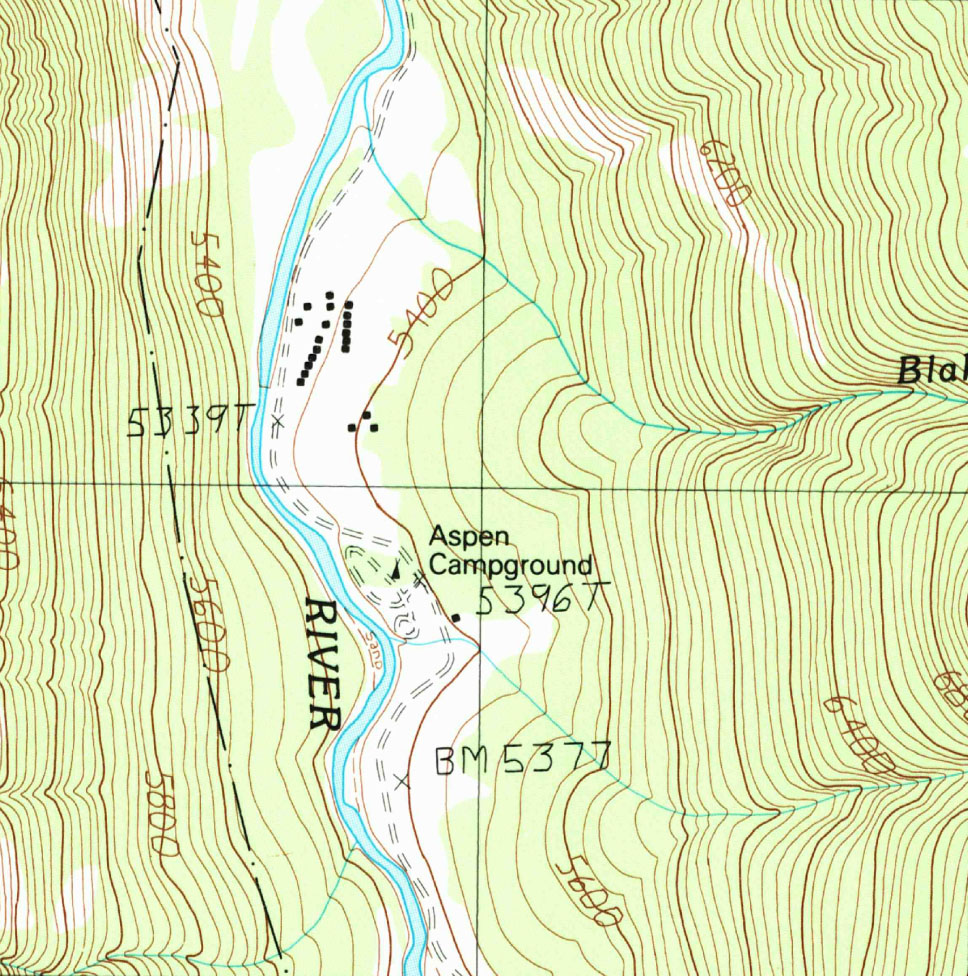
\includegraphics[scale=.65]{figures/MT_ChromeMountain_topo_small.pdf}
%}

Given a function $z=f(x,y)$, we can draw a ``topographical map'' of $f$ by drawing \textbf{level curves} (or, contour lines). A level curve at $z=c$ is a curve in the $x$-$y$ plane such that for all points $(x,y)$ on the curve, $f(x,y) = c$. 

When drawing level curves, it is important that the $c$ values are spaced equally apart as that gives the best insight to how quickly the ``elevation'' is changing. Examples will help one understand this concept.\\

\example{ex_levelcurve1}{Drawing Level Curves}{
Let $\ds f(x,y) = \sqrt{1-\frac{x^2}9-\frac{y^2}4}$. Find the level curves of $f$ for $c=0$, $0.2$, $0.4$, $0.6$, $0.8$ and $1$.}
{Consider first $c=0$. The level curve for $c=0$ is the set of all points $(x,y)$ such that $0=\sqrt{1-\frac{x^2}9-\frac{y^2}4}$. Squaring both sides  gives us
\[
\frac{x^2}9+\frac{y^2}4=1,
\]
an ellipse centred at $(0,0)$ with horizontal major axis of length 6 and minor axis of length 4. Thus for any point $(x,y)$ on this curve, $f(x,y) = 0$.

Now consider the level curve for $c=0.2$
\begin{align*}
0.2 &= \sqrt{1-\frac{x^2}9-\frac{y^2}4}\\
0.04 &= 1-\frac{x^2}9-\frac{y^2}4\\
\frac{x^2}9+\frac{y^2}4 &=0.96\\
\frac{x^2}{8.64}+\frac{y^2}{3.84} &=1.
\end{align*}
This is also an ellipse, where $a = \sqrt{8.64}\approx 2.94$ and $b=\sqrt{3.84}\approx 1.96$.

In general, for $z=c$, the level curve is:
\begin{align*}
c &= \sqrt{1-\frac{x^2}9-\frac{y^2}4}\\
c^2 &= 1-\frac{x^2}9-\frac{y^2}4\\
\frac{x^2}9+\frac{y^2}4 &=1-c^2\\
\frac{x^2}{9(1-c^2)}+\frac{y^2}{4(1-c^2)} &=1,
\end{align*}
ellipses that are decreasing in size as $c$ increases. A special case is when $c=1$; there the ellipse is just the point $(0,0)$. 

The level curves are shown in Figure \ref{fig:levelcurves1}(a). Note how the level curves for $c=0$ and $c=0.2$ are very, very close together: this indicates that $f$ is growing rapidly along those curves.

\mtable{.71}{Graphing the level curves in Example \ref{ex_levelcurve1}.}{fig:levelcurves1}{%
\begin{tabular}{c}
\myincludegraphics{figures/figlevelcurve1b}\\
(a)\\[10pt]
\myincludegraphicsthree{width=150pt,3Dmenu,activate=onclick,deactivate=pageinvisible,
3Droll=0,
3Dortho=0.004999999888241291,
3Dc2c=0.6562340259552002 0.7273486256599426 0.20080043375492096,
3Dcoo=2.348435640335083 -6.5163373947143555 66.12745666503906,
3Droo=129.99999641808185,
3Dlights=Headlamp,add3Djscript=asylabels.js}{width=150pt}{figures/figlevelcurve1}\\
%\myincludegraphics[scale=1.25,trim=3mm 0mm 3mm 0mm,clip]{figures/figlevelcurve1}\\
(b)
\end{tabular}
}

In Figure \ref{fig:levelcurves1}(b), the curves are drawn on a graph of $f$ in space. Note how the elevations are evenly spaced. Near the level curves of $c=0$ and $c=0.2$ we can see that $f$ indeed is growing quickly.
}\\

\example{ex_levelcurves2}{Analyzing Level Curves}{
Let $\ds f(x,y) = \frac{x+y}{x^2+y^2+1}$. Find the level curves for $z=c$.}
{We begin by setting $f(x,y)=c$ for an arbitrary $c$ and seeing if algebraic manipulation of the equation reveals anything significant.
\begin{align*}
\frac{x+y}{x^2+y^2+1} &= c \\
x+y &= c(x^2+y^2+1).
\intertext{We recognize this as a circle, though the center and radius are not yet clear. By completing the square, we can obtain:}
\left(x-\frac{1}{2c}\right)^2+\left(y-\frac1{2c}\right)^2&=\frac{1}{2c^2}-1,
\end{align*}
a circle centred at $\big(1/(2c),1/(2c)\big)$ with radius $\sqrt{1/(2c^2)-1}$, where $\vert c\rvert <1/\sqrt{2}$. The level curves for $c=\pm 0.2,\ \pm 0.4$ and $\pm0.6$ are sketched in Figure \ref{fig:levelcurves2}(a). To help illustrate ``elevation,'' we use thicker lines for $c$ values near 0, and dashed lines indicate where $c<0$. 

There is one special level curve, when $c=0$. The level curve in this situation is $x+y=0$, the line $y=-x$.

In Figure \ref{fig:levelcurves2}(b) we see a graph of the surface. Note how the $y$-axis is pointing away from the viewer to more closely resemble the orientation of the level curves in (a). 

\mtable{.27}{Graphing the level curves in Example \ref{ex_levelcurves2}.}{fig:levelcurves2}{%
\begin{tabular}{c}
\myincludegraphics{figures/figlevelcurve2b}\\
(a)\\[10pt]
%\myincludegraphics[scale=1.2,trim=0mm 5mm 0mm 0mm,clip]{figures/figlevelcurve2}\\
{\myincludegraphicsthree{width=150pt,3Dmenu,activate=onclick,deactivate=pageinvisible,
3Droll=0.25732633644359904,
3Dortho=0.004999999888241291,
3Dc2c=0.5196654200553894 -0.7088789939880371 0.4769051671028137,
3Dcoo=-0.7249413728713989 1.7016432285308838 3.277412176132202,
3Droo=130.00000541214214,
3Dlights=Headlamp,add3Djscript=asylabels.js}{width=150pt}{figures/figlevelcurve2}}\\
(b)
\end{tabular}
}



%\mfigurethree[width=150pt,3Dmenu,activate=onclick,deactivate=pageinvisible,
%3Droll=0,
%3Dc2c=1 -1.5 1,
%3Dcoo=0 0 0,
%3Droo=130,
%3Dortho=.005,
%3Dlights=Headlamp,add3Djscript=asylabels.js]{.4}{Visualizing the solid shown from Example \ref{ex_doublepol4}.}{fig:doublepol4}{figures/figlevelcurve2_3D} 

Seeing the level curves helps us understand the graph. For instance, the graph does not make it clear that one can ``walk'' along the line $y=-x$ without elevation change, though the level curve does.
}\\

\noindent\textbf{\large Functions of Three Variables}\\

We extend our study of multivariable functions to functions of three variables. (One can make a function of as many variables as one likes; we limit our study to three variables.)

\definition{def:multi3}{Function of Three Variables}
{Let $D$ be a subset of $\mathbb{R}^3$. A \textbf{function $f$ of three variables} is a rule that assigns each triple $(x,y,z)$ in $D$ a value $w=f(x,y,z)$ in $\mathbb{R}$. $D$ is the \textbf{domain} of $f$; the set of all outputs of $f$ is the \textbf{range}.
\index{multivariable function}\index{function!of three variables}\index{multivariable function!domain}\index{multivariable function!range}
}

Note how this definition closely resembles that of Definition \ref{def:multi2}.\\

\example{ex_multi3}{Understanding a function of three variables}{
Let $\ds f(x,y,z) =  \frac{x^2+z+3\sin y}{x+2y-z}.$ Evaluate $f$ at the point $(3,0,2)$ and find the domain and range of $f$.}
{$\ds f(3,0,2) = \frac{3^2+2+3\sin 0}{3+2(0)-2} = 11.$

As the domain of $f$ is not specified, we take it to be the set of all triples $(x,y,z)$ for which $f(x,y,z)$ is defined. As we cannot divide by $0$, we find the domain $D$ is 
\[
D = \{(x,y,z)\ |\ x+2y-z\neq 0\}.
\]
We recognize that the set of all points in $\mathbb{R}^3$ that \textit{are not} in $D$ form a plane in space that passes through the origin (with normal vector $\la 1,2,-1\ra$). 

We determine the range $R$ is $\mathbb{R}$; that is, all real numbers are possible outputs of $f$. There is no set way of establishing this. Rather, to get numbers near 0 we can let $y=0$ and choose $z \approx -x^2$. To get numbers of arbitrarily large magnitude, we can let $z\approx x+2y$. 
}\\

%\clearpage
\noindent\textbf{\large Level Surfaces}\\

It is very difficult to produce a meaningful graph of a function of three variables. A function of \textit{one} variable is a \textit{curve} drawn in \textit{2} dimensions; a function of \textit{two} variables is a \textit{surface} drawn in \textit{3} dimensions; a function of \textit{three} variables is a \textit{hypersurface} drawn in \textit{4} dimensions.\index{multivariable function!level surface}\index{level surface}

There are a few techniques one can employ to try to ``picture'' a graph of three variables. One is an analogue of level curves: \textbf{level surfaces}. Given $w=f(x,y,z)$, the level surface at $w=c$ is the surface in space formed by all points $(x,y,z)$ where $f(x,y,z)=c$. \\

\example{ex_multi4}{Finding level surfaces}{
If a point source $S$ is radiating energy, the intensity $I$ at a given point $P$ in space is inversely proportional to the square of the distance between $S$ and $P$. That is, when $S=(0,0,0)$,  $\ds I(x,y,z) = \frac{k}{x^2+y^2+z^2}$ for some constant $k$.

Let $k=1$; find the level surfaces of $I$.}
{We can (mostly) answer this question using ``common sense.'' If energy (say, in the form of light) is emanating from the origin, its intensity will be the same at all points equidistant from the origin. That is, at any point on the surface of a sphere centred at the origin, the intensity should be the same. Therefore, the level surfaces are spheres.

We now find this mathematically. The level surface at $I=c$ is defined by 
\begin{align*}
c &= \frac{1}{x^2+y^2+z^2}.
\intertext{A small amount of algebra reveals}
x^2+y^2+z^2 &= \frac1c.
\end{align*}
Given an intensity $c$, the level surface $I=c$ is a sphere of radius $1/\sqrt{c}$, centred at the origin. 

\mtable{.7}{A table of $c$ values and the corresponding radius $r$ of the spheres of constant value in Example \ref{ex_multi4}.}{fig:multi4}{
\begin{tabular}{cc}
$c$ & $r$ \\ \hline
16. & 0.25 \\
 8. & 0.35 \\
 4. & 0.5 \\
 2. & 0.71 \\
 1. & 1. \\
 0.5 & 1.41 \\
 0.25 & 2. \\
 0.125 & 2.83 \\
 0.0625 & 4. \\
\end{tabular}
}

Figure \ref{fig:multi4} gives a table of the radii of the spheres for given $c$ values. Normally one would use equally spaced $c$ values, but these values have been chosen purposefully. At a distance of 0.25 from the point source, the intensity is 16; to move to a point of half that intensity, one just moves out 0.1 to 0.35 -- not much at all. To again halve the intensity, one moves 0.15, a little more than before.

Note how each time the intensity if halved, the distance required to move away grows. We conclude that the closer one is to the source, the more rapidly the intensity changes.
}\\

\enlargethispage{2\baselineskip}
In the next section we apply the concepts of limits to functions of two or more variables.

\printexercises{exercises/12_01_exercises}

\section{Limits and Continuity of Multivariable Functions}\label{sec:multi_limit}

We continue with the pattern we have established in this text: after defining a new kind of function, we apply calculus ideas to it. The previous section defined functions of two and three variables; this section investigates what it means for these functions to be ``continuous.''

We begin with a series of definitions. We are used to ``open intervals'' such as $(1,3)$, which represents the set of all $x$ such that $1<x<3$,  and ``closed intervals'' such as $[1,3]$, which represents the set of all $x$ such that $1\leq x\leq 3$. We need analogous definitions for open and closed sets in the $x$-$y$ plane.

\definition{def:open}{\parbox[t]{225pt}{Open Disk, Boundary and Interior Points, Open and Closed Sets, Bounded Sets}}
{An \textbf{open disk} $B$ in $\mathbb{R}^2$ centered at $(x_0,y_0)$ with radius $r$ is the set of all points $(x,y)$ such that $\ds\sqrt{(x-x_0)^2+(y-y_0)^2} < r$. \\

Let $S$ be a set of points in $\mathbb{R}^2$. A point $P$ in $\mathbb{R}^2$ is a \textbf{boundary point} of $S$  if all open disks centered at $P$ contain both points in $S$ and points not in $S$.\\

A point $P$ in $S$ is an \textbf{interior point} of $S$ if there is an open disk centered at $P$ that contains only points in $S$. \\

A set $S$ is \textbf{open} if every point in $S$ is an interior point.\\

A set $S$ is \textbf{closed} if it contains all of its boundary points.\\

A set $S$ is \textbf{bounded} if there is an $M>0$ such that the open disk, centered at the origin with radius $M$, contains $S$. A set that is not bounded is \textbf{unbounded}.
\index{open}\index{closed}\index{open disk}\index{closed disk}\index{boundary point}\index{interior point}\index{bounded set}\index{unbounded set}
}

Figure \ref{fig:multilimit_intro} shows several sets in the $x$-$y$ plane. In each set, point $P_1$ lies on the boundary of the set as all open disks centered there contain both points in, and not in, the set. In contrast, point $P_2$ is an interior point for there is an open disk centered there that lies entirely within the set.
\mtable{.6}{Illustrating open and closed sets in the $x$-$y$ plane.}{fig:multilimit_intro}{%
\begin{tabular}{c}
\myincludegraphics{figures/figmultilimit_introa}\\
(a)\\[10pt]
\myincludegraphics{figures/figmultilimit_introb}\\
(b)\\[10pt]
\myincludegraphics{figures/figmultilimit_introc}\\
(c)\\[10pt]
\end{tabular}
}

The set depicted in Figure \ref{fig:multilimit_intro}(a) is a closed set as it contains all of its boundary points. The set in (b) is open, for all of its points are interior points (or, equivalently, it does not contain any of its boundary points). The set in (c) is neither open nor closed as it contains  some of its boundary points.\\


\example{ex_multilimit1}{Determining open/closed, bounded/unbounded}{
Determine if the domain of the function $f(x,y)=\sqrt{1-\frac{x^2}9-\frac{y^2}4}$ is open, closed, or neither, and if it is bounded.}
{This domain of this function was found in Example \ref{ex_multi2} to be $D = \{(x,y)\ |\ \frac{x^2}9+\frac{y^2}4\leq 1\}$, the region \textit{bounded} by the ellipse $\frac{x^2}9+\frac{y^2}4=1$. Since the region includes the boundary (indicated by the use of ``$\leq$''), the set contains all of its boundary points and hence is closed. The region is bounded as a disk of radius 4, centered at the origin, contains $D$.
}\\
\pagebreak

\example{ex_multilimit2}{Determining open/closed, bounded/unbounded}{
Determine if the domain of $f(x,y) = \frac1{x-y}$ is open, closed, or neither.}
{As we cannot divide by 0, we find the domain to be $D = \{(x,y)\ |\ x-y\neq 0\}$. In other words, the domain is the set of all points $(x,y)$ \emph{not} on the line $y=x$. 

\mfigure{.75}{Sketching the domain of the function in Example \ref{ex_multilimit2}.}{fig:multilimit2}{figures/figmultilimit2}
The domain is sketched in Figure \ref{fig:multilimit2}. Note how we can draw an open disk around any point in the domain that lies entirely inside the domain, and also note how the only boundary points of the domain are the points on the line $y=x$. We conclude the domain is an open set. The set is unbounded.
}\\

\noindent\textbf{\large Limits}\\

Recall a pseudo--definition of the limit of a function of one variable: ``$\ds \lim_{x\to c}f(x) = L$'' means that if $x$ is ``really close'' to $c$, then $f(x)$ is ``really close'' to $L$. A similar pseudo--definition holds for functions of two variables. We'll say that 
%\enlargethispage{3\baselineskip}

\begin{center}
``$\ds \lim_{(x,y)\to (x_0,y_0)} f(x,y) = L$'' 
\end{center}
means ``if the point $(x,y)$ is really close to the point $(x_0,y_0)$, then $f(x,y)$ is really close to $L$.'' The formal definition is given below.

\mfigurethree{width=150pt,3Dmenu,activate=onclick,deactivate=onclick,
3Droll=0.12234160136132792,
3Dortho=0.004824123345315456,
3Dc2c=0.9118747115135193 -0.1974218785762787 0.35987377166748047,
3Dcoo=21.82058334350586 66.31769561767578 47.81545639038086,
3Droo=149.99999973566392,
3Dlights=Headlamp,add3Djscript=asylabels.js}{scale=1.25}{.25}{\textbf{Illustrating the definition of a limit.} The open disk in the $x$-$y$ plane has radius $\delta$. Let $(x,y)$ be any point in this disk; $f(x,y)$ is within $\epsilon$ of $L$.}{fig:multilimitdef}{figures/figmultilimit_def}

\definition{def:multilimit}{Limit of a Function of Two Variables}
{Let $S$ be an open set containing $(x_0,y_0)$, and let $f$ be a function of two variables defined on $S$, except possibly at $(x_0,y_0)$. 
%Let $f(x,y)$ be a function of two variables and let $(x_0,y_0)$ be a point in the domain of $f$. 
The \textbf{limit} of $f(x,y)$ as $(x,y)$ approaches $(x_0,y_0)$ is $L$, denoted $$\ds \lim_{(x,y)\to (x_0,y_0)} f(x,y) = L,$$
means that given any $\epsilon>0$, there exists $\delta>0$ such that for all  $(x,y)\neq (x_0,y_0)$, if $(x,y)$ is in the open disk centered at $(x_0,y_0)$ with radius $\delta$, then $|f(x,y) - L|<\epsilon.$
\index{limit!of multivariable function}\index{multivariable function!limit}
}


The concept behind Definition \ref{def:multilimit} is sketched in Figure \ref{fig:multilimitdef}. Given $\epsilon>0$, find $\delta>0$ such that if $(x,y)$ is any point in the open disk centred at $(x_0,y_0)$ in the $x$-$y$ plane with radius $\delta$, then $f(x,y)$ should be within $\epsilon$ of $L$. 

\pagebreak

Computing limits using this definition is rather cumbersome. The following theorem allows us to evaluate limits much more easily.


%\mfigure[scale=1.25]{.77}{\textbf{Illustrating the definition of a limit.} The open disk in the $x$-$y$ plane has radius $\delta$. Let $(x,y)$ be any point in this disk; $f(x,y)$ is within $\epsilon$ of $L$.}{fig:multilimitdef}{figures/figmultilimit_def}


\setboxwidth{0pt}
\theorem{thm:multi_limit_algebra}{Basic Limit Properties of Functions of Two Variables}{%\small
Let $b$, $x_0$, $y_0$, $L$ and $K$ be real numbers,  let $n$ be a positive integer, and let $f$ and $g$ be functions with the following limits:
$$\lim_{(x,y)\to (x_0,y_0)}f(x,y) = L \quad \text{\ and\ } \lim_{(x,y)\to (x_0,y_0)} g(x,y) = K.$$
The following limits hold.
\index{limit!of multivariable function}\index{limit!properties}\index{multivariable function!limit}
\begin{enumerate}
\item \parbox{80pt}{Constants:} $\displaystyle \lim_{(x,y)\to (x_0,y_0)} b = b$
\item	\parbox{80pt}{Identity }	$\displaystyle \lim_{(x,y)\to (x_0,y_0)} x = x_0$;\qquad $\displaystyle \lim_{(x,y)\to (x_0,y_0)} y = y_0$
\item	\parbox{80pt}{Sums/Differences:} $\displaystyle \lim_{(x,y)\to (x_0,y_0)}\big(f(x,y)\pm g(x,y)\big) = L\pm K$
\item	\parbox{80pt}{Scalar Multiples:}	$\displaystyle \lim_{(x,y)\to (x_0,y_0)} b\cdot f(x,y) = bL$
\item	\parbox{80pt}{Products:}	$\displaystyle \lim_{(x,y)\to (x_0,y_0)} f(x,y)\cdot g(x,y) = LK$
\item	\parbox{80pt}{Quotients:} $\displaystyle \lim_{(x,y)\to (x_0,y_0)} f(x,y)/g(x,y) = L/K$, ($K\neq 0)$
\item	\parbox{80pt}{Powers:} 	$\displaystyle \lim_{(x,y)\to (x_0,y_0)} f(x,y)^n = L^n$
%\item	\parbox{80pt}{Roots:}		\parbox[t]{185pt}{$\displaystyle \lim_{(x,y)\to (x_0,y_0)} \sqrt[n]{f(x,y)} = \sqrt[n]{L}$}% \qquad \small (if $n$ is even then $L$ must be greater than 0; when $n$ is odd, it is true for all $L$.)}

\end{enumerate}
}
\restoreboxwidth

This theorem, combined with Theorems \ref{thm:poly_rat} and \ref{thm:lim_continuous} of Section \ref{sec:limit_analytically}, allows us to evaluate many limits.\\

\example{ex_multilimit3}{Evaluating a limit}{
Evaluate the following limits:
$$1. \lim_{(x,y)\to (1,\pi)} \frac yx + \cos(xy) \qquad\qquad 2. \lim_{(x,y)\to (0,0)} \frac{3xy}{x^2+y^2}$$
}
{\begin{enumerate}
	\item The aforementioned theorems allow us to simply evaluate $y/x+\cos(xy)$ when $x=1$ and $y=\pi$. If an indeterminate form is returned, we must do more work to evaluate the limit; otherwise, the result is the limit. Therefore
	\begin{align*}
	\lim_{(x,y)\to (1,\pi)} \frac yx + \cos(xy)  &= \frac\pi{1}+\cos \pi \\
		&= \pi -1.
	\end{align*}
	\item		We attempt to evaluate the limit by substituting 0 in for $x$ and $y$, but the result is the indeterminate form ``$0/0$.'' To evaluate this limit, we must ``do more work,'' but we have not yet learned what ``kind'' of work to do. Therefore we cannot yet evaluate this limit.
\end{enumerate}
\vskip -1.5\baselineskip
}\\

When dealing with functions of a single variable we also considered one--sided limits and stated
$$\lim_{x\to c}f(x) = L \quad\text{ if, and only if,}\quad \lim_{x\to c^+}f(x) =L \quad\textbf{ and}\quad \lim_{x\to c^-}f(x) =L.$$
That is, the limit is $L$ if and only if $f(x)$ approaches $L$ when $x$ approaches $c$ from \textbf{either} direction, the left or the right.

In the plane, there are infinite directions from which $(x,y)$ might approach $(x_0,y_0)$. In fact, we do not have to restrict ourselves to approaching $(x_0,y_0)$ from a particular direction, but rather we can approach that point along a path that is not a straight line. It is possible to arrive at different limiting values by approaching $(x_0,y_0)$ along different paths. If this happens, we say that $\ds \lim_{(x,y)\to(x_0,y_0) } f(x,y)$ does not exist (this is analogous to the left and right hand limits of single variable functions not being equal).

Our theorems tell us that we can evaluate most limits quite simply, without worrying about  paths. When indeterminate forms arise, the limit may or may not exist. If it does exist, it can be difficult to prove this as we need to show the same limiting value is obtained regardless of the path chosen. The case where the limit does not exist is often easier to deal with, for we can often pick two paths along which the limit is different.\\

%it can be difficult to show that the limit exists, for we need to show that the same limiting value is obtained regardless of the path taken.  we can often evaluate the limit along specific paths. If any of these limits differ, we say that \emph{the} limit does not exist.\\

\example{ex_multilimit4}{Showing limits do not exist}{
\begin{enumerate}
	\item Show $\ds \lim_{(x,y)\to (0,0)} \frac{3xy}{x^2+y^2}$ does not exist by finding the limits along the lines $y=mx$.
	\item	Show $\ds \lim_{(x,y)\to (0,0)} \frac{\sin(xy)}{x+y}$ does not exist by finding the limit along the path $y=-\sin x$. 	
\end{enumerate}
}
{\begin{enumerate}
	\item Evaluating $\ds \lim_{(x,y)\to (0,0)} \frac{3xy}{x^2+y^2}$ along the lines $y=mx$ means replace all $y$'s with $mx$ and evaluating the resulting limit:
	\begin{align*}
	\lim_{(x,mx)\to (0,0)} \frac{3x(mx)}{x^2+(mx)^2} &=\lim_{x\to 0} \frac{3mx^2}{x^2(m^2+1)}\\
				&= \lim_{x\to 0} \frac{3m}{m^2+1}\\
				&= \frac{3m}{m^2+1}.
	\end{align*}
	While the limit exists for each choice of $m$, we get a \emph{different} limit for each choice of $m$. That is, along different lines we get differing limiting values, meaning \emph{the} limit does not exist.
	
	\item		Let $f(x,y) = \frac{\sin(xy)}{x+y}$. We are to show that $\ds \lim_{(x,y)\to (0,0)} f(x,y)$ does not exist by finding the limit along the path $y=-\sin x$. First, however, consider the limits found along the lines $y=mx$ as done above.
	\begin{align*}
	\lim_{(x,mx)\to (0,0)} \frac{\sin\big(x(mx)\big)}{x+mx} &= \lim_{x\to 0} \frac{\sin (mx^2)}{x(m+1)} \\
	&= \lim_{x\to 0} \frac{\sin(mx^2)}{x}\cdot\frac1{m+1}.
	\end{align*}
	By applying L'H\^opital's Rule, we can show this limit is 0 \emph{except} when $m=-1$, that is, along the line $y=-x$. This line is not in the domain of $f$, so we have found the following fact: along every line $y=mx$ in the domain of $f$, $\ds \lim_{(x,y)\to(0,0)} f(x,y)=0$. %Along this line, $f(x,y)$ is not defined, so it stands to reason that a limit along this line does not exist.
%\drawexampleline
	
	Now consider the limit along the path $y=-\sin x$:
	\begin{align*}
	\lim_{(x,-\sin x)\to (0,0)} \frac{\sin\big(-x\sin x\big)}{x-\sin x} &= \lim_{x\to0} \frac{\sin\big(-x\sin x\big)}{x-\sin x}
	\end{align*}
	Now apply L'H\^opital's Rule twice:
	\small
	\begin{align*}
	 \quad &= \lim_{x\to 0}\frac{\cos\big(-x\sin x\big)(-\sin x-x\cos x)}{1-\cos x} \quad \left(\text{``}= 0/0\text{''}\right)\\
	&= \lim_{x\to 0}\frac{-\sin\big(-x\sin x\big)(-\sin x-x\cos x)^2+\cos\big(-x\sin x\big)(-2\cos x+x\sin x)}{\sin x}\\
	&= \text{``2/0''} \Rightarrow \text{the limit does not exist.}
	\end{align*}
	\normalsize
Step back and consider what we have just discovered. Along any line $y=mx$ in the domain of the $f(x,y)$, the limit is 0. However, along the path $y=-\sin x$, which lies in the domain of  $f(x,y)$ for all $x\neq 0$, the limit does not exist. Since the limit is not the same along every path to $(0,0)$, we say $\ds \lim_{(x,y)\to (0,0)}\frac{\sin(xy)}{x+y}$ does not exist.
\end{enumerate}
\vskip -1.5\baselineskip
}\\

\example{ex_multilimit5}{Finding a limit}{
Let $\ds f(x,y) = \frac{5x^2y^2}{x^2+y^2}$. Find $\ds\lim_{(x,y)\to (0,0)}  f(x,y) .$
}
{It is relatively easy to show that along any line $y=mx$, the limit is 0. This is not enough to prove that the limit exists, as demonstrated in the previous example, but it tells us that if the limit does exist then it must be 0.

To prove the limit is 0, we apply Definition \ref{def:multilimit}. Let $\epsilon >0$ be given. We want to find $\delta >0$ such that if $\sqrt{(x-0)^2+(y-0)^2} <\delta$, then $|f(x,y)-0| <\epsilon$.

Set $\delta < \sqrt{\epsilon/5}$. Note that $\ds \left|\frac{5y^2}{x^2+y^2}\right| <5$ for all $(x,y)\neq (0,0)$, and that if $\sqrt{x^2+y^2} <\delta$, then $x^2<\delta^2$.

Let $\sqrt{(x-0)^2+(y-0)^2} = \sqrt{x^2+y^2}<\delta$. Consider $|f(x,y)-0|$:
\begin{align*}
|f(x,y)-0| &= \left|\frac{5x^2y^2}{x^2+y^2}-0\right| \\
				&= \left|x^2\cdot\frac{5y^2}{x^2+y^2}\right|\\
				&< \delta^2\cdot 5 \\
				&< \frac{\epsilon}{5}\cdot 5 \\
				&= \epsilon.
\end{align*}
Thus if $\sqrt{(x-0)^2+(y-0)^2}<\delta$ then $|f(x,y)-0|<\epsilon$, which is what we wanted to show. Thus $\ds \lim_{(x,y)\to(0,0)} \frac{5x^2y^2}{x^2+y^2} = 0$.
}\\
%\pagebreak

\noindent\textbf{\large Continuity}\\

Definition \ref{def:continuous} defines what it means for a function of one variable to be continuous. In brief, it meant that the graph of the function did not have breaks, holes, jumps, etc. We define continuity for functions of two variables in a similar way as we did for functions of one variable.

\definition{def:multi_continuous}{Continuous}
{Let a function $f(x,y)$ be defined on an open disk $B$ containing the point $(x_0,y_0)$. 

\begin{enumerate}
	\item $f$ is \textbf{continuous} at $(x_0,y_0)$ if $\ds\lim_{(x,y)\to(x_0,y_0)} f(x,y) = f(x_0,y_0)$.
	\index{continuous function}\index{multivariable function!continuity}
	\item	$f$ is \textbf{continuous on $B$} if $f$ is continuous at all points in $B$. If $f$ is continuous at all points in $\mathbb{R}^2$, we say that $f$ is \textbf{continuous everywhere}.
\end{enumerate}
}

\example{ex_multicont1}{Continuity of a function of two variables}{
Let $\ds f(x,y) = \left\{ \begin{array}{rl} \frac{\cos y\sin x}{x} & x\neq 0 \\
																						\cos y & x=0
													\end{array} \right.$. Is $f$ continuous at $(0,0)$? Is $f$ continuous everywhere?
}
{To determine if $f$ is continuous at $(0,0)$, we need to compare $\ds\lim_{(x,y)\to (0,0)} f(x,y)$ to $f(0,0)$. 

Applying the definition of $f$, we see that $f(0,0) = \cos 0 = 1$. 

We now consider the limit $\ds \lim_{(x,y)\to (0,0)} f(x,y)$. Substituting $0$ for $x$ and $y$ in $(\cos y\sin x)/x$ returns the indeterminate form ``0/0'', so we need to do more work to evaluate this limit.

Consider two related limits: $\ds \lim_{(x,y)\to (0,0)} \cos y$ and $\ds \lim_{(x,y)\to(0,0)} \frac{\sin x}x$. The first limit does not contain $x$, and since $\cos y$ is continuous, $$\ds \lim_{(x,y)\to (0,0)} \cos y =\lim_{y\to 0} \cos y = \cos 0 = 1.$$

The second limit does not contain $y$. By Theorem \ref{thm:special_limits} we can say
$$\lim_{(x,y)\to (0,0)} \frac{\sin x}{x} = \lim_{x\to 0} \frac{\sin x}{x} = 1.$$
Finally, Theorem \ref{thm:multi_limit_algebra} of this section states that we can combine these two limits as follows:
\begin{align*}
\lim_{(x,y)\to (0,0)} \frac{\cos y\sin x}{x} &= \lim_{(x,y)\to (0,0)} (\cos y)\left(\frac{\sin x}{x}\right) \\ 
&=\left(\lim_{(x,y)\to (0,0)} \cos y\right)\left(\lim_{(x,y)\to (0,0)} \frac{\sin x}{x}\right) \\
  &= (1)(1)\\
	&=1.
\end{align*}

We have found that $\ds \lim_{(x,y)\to (0,0)} \frac{\cos y\sin x}{x} = f(0,0)$, so $f$ is continuous at $(0,0)$.

A similar analysis shows that $f$ is continuous at all points in $\mathbb{R}^2$. As long as $x\neq0$, we can evaluate the limit directly; when $x=0$, a similar analysis shows that the limit is $\cos y$. Thus we can say that $f$ is continuous everywhere. A graph of $f$ is given in Figure \ref{fig:multicont1}. Notice how it has no breaks, jumps, etc.
\mfigurethree{width=150pt,3Dmenu,activate=onclick,deactivate=onclick,
3Droll=1.3976649182325884,
3Dortho=0.005226649809628725,
3Dc2c=0.6559564471244812 0.554935097694397 0.5116328597068787,
3Dcoo=-1.2457355260849 0.0923926830291748 4.189182281494141,
3Droo=129.99999868169073,
3Dlights=Headlamp,add3Djscript=asylabels.js}{scale=1.25}{.5}{A graph of $f(x,y)$ in Example \ref{ex_multicont1}.}{fig:multicont1}{figures/figmulticont1}
%\mfigure[scale=1.25]{.8}{A graph of $f(x,y)$ in Example \ref{ex_multicont1}.}{fig:multicont1}{figures/figmulticont1}
}\\

The following theorem is very similar to Theorem \ref{thm:continuity_algebra}, giving us ways to combine continuous functions to create other continuous functions.

\theorem{thm:multi_continuous_prop}{Properties of Continuous Functions}
{Let $f$ and $g$ be continuous on an open disk $B$, let $c$ be a real number, and let $n$ be a positive integer. The following functions are continuous on $B$.
\index{continuous function!properties}\index{multivariable function!continuity}
		\begin{enumerate}
		\item		\parbox{80pt}{Sums/Differences:}	$f\pm g$
		\item		\parbox{80pt}{Constant Multiples:}	$c\cdot f$
		\item		\parbox{80pt}{Products:}	$f\cdot g$
		\item		\parbox{80pt}{Quotients:}	$f/g$ \qquad {\small (as longs as $g\neq 0$ on $B$)}
		\item		\parbox{80pt}{Powers:}	$f\,^n$
		\item		\parbox{80pt}{Roots:}	$\sqrt[n]{f}$ \qquad \parbox[t]{150pt}{\small (if $n$ is even then $f\geq 0$ on $B$; if $n$ is odd, then true for all values of $f$ on $B$.)}
		\item		\parbox{80pt}{Compositions:}\parbox[t]{185pt}{Adjust the definitions of $f$ and $g$ to: Let $f$ be continuous on $B$, where the range of $f$ on $B$ is $J$, and let $g$ be a single variable function that is continuous on $J$. Then $g\circ f$, i.e., $g(f(x,y))$, is continuous on $B$.}
		\end{enumerate}
}
\enlargethispage{\baselineskip}

\example{ex_multicont2}{Establishing continuity of a function}{
Let $f(x,y) = \sin (x^2\cos y)$. Show $f$ is continuous everywhere.}
{We will apply both Theorems \ref{thm:continuity_algebra} and \ref{thm:multi_continuous_prop}. Let $f_1(x,y) = x^2$. Since $y$ is not actually used in the function, and polynomials are continuous (by Theorem \ref{thm:continuity_algebra}), we conclude $f_1$ is continuous everywhere. A similar statement can be made about $f_2(x,y) = \cos y$. Part 3 of Theorem \ref{thm:multi_continuous_prop} states that $f_3=f_1\cdot f_2$ is continuous everywhere, and Part 7 of the theorem states the composition of sine with $f_3$ is continuous: that is, $\sin (f_3) = \sin(x^2\cos y)$ is continuous everywhere.
}\\
\pagebreak

\noindent\textbf{\large Functions of Three Variables}\\

The definitions and theorems given in this section can be extended in a natural way to definitions and theorems about functions of three (or more) variables. We cover the key concepts here; some terms from Definitions \ref{def:open} and \ref{def:multi_continuous} are not redefined but their analogous meanings should be clear to the reader.

\setboxwidth{20pt}
\definition{def:multi3defs}{Open Balls, Limit, Continuous}
{ 
\begin{enumerate}
\item An \textbf{open ball} in $\mathbb{R}^3$ centered at $(x_0,y_0,z_0)$ with radius $r$ is the set of all points $(x,y,z)$ such that $\sqrt{(x-x_0)^2+(y-y_0)^2+(z-z_0)^2} = r$.
\index{multivariable function!limit}\index{limit!of multivariable function}\index{multivariable function!continuity}\index{open ball}
\\

\item Let $D$ be an open set in $\mathbb{R}^3$ containing $(x_0,y_0,z_0)$, and let $f(x,y,z)$ be a function of three variables defined on $D$, except possibly at  $(x_0,y_0,z_0)$. The \textbf{limit} of $f(x,y,z)$ as $(x,y,z)$ approaches $(x_0,y_0,z_0)$ is $L$, denoted 
$$\lim_{(x,y,z)\to (x_0,y_0,z_0)} f(x,y,z) = L,$$
means that given any $\epsilon >0$, there is a $\delta >0$ such that for all  $(x,y,z)\neq(x_0,y_0,z_0)$, if $(x,y,z)$ is in the open ball centered at $(x_0,y_0,z_0)$ with radius $\delta$, then $|f(x,y,z) - L|< \epsilon$.\\

\item Let $f(x,y,z)$ be defined on an open ball $B$ containing $(x_0,y_0,z_0)$. $f$ is \textbf{continuous} at $(x_0,y_0,z_0)$ if $\ds \lim_{(x,y,z)\to (x_0,y_0,z_0)} f(x,y,z) = f(x_0,y_0,z_0)$.
\end{enumerate}
}
\restoreboxwidth

These definitions can also be extended naturally to apply to functions of four or more variables. Theorem \ref{thm:multi_continuous_prop} also applies to function of three or more variables, allowing us to say that the function $$\ds f(x,y,z) = \frac{e^{x^2+y}\sqrt{y^2+z^2+3}}{\sin (xyz)+5}$$ is continuous everywhere.

When considering single variable functions, we studied limits, then continuity, then the derivative. In our current study of multivariable functions, we have studied limits and continuity. In the next section we study derivation, which takes on a slight twist as we are in a multivarible context.

\printexercises{exercises/12_02_exercises}
\section{Partial Derivatives}\label{sec:partial_derivatives}

Let $y$ be a function of $x$. We have studied in great detail the derivative of $y$ with respect to $x$, that is, $\frac{dy}{dx}$, which measures the rate at which $y$ changes with respect to $x$. Consider now $z=f(x,y)$. It makes sense to want to know how $z$ changes with respect to $x$ and/or $y$. This section begins our investigation into these rates of change.

Consider the function $z=f(x,y) = x^2+2y^2$, as graphed in Figure \ref{fig:partialintro}(a). By fixing $y=2$, we focus our attention to all points on the surface where the $y$-value is 2, shown in both parts (a) and (b) of the figure. These points form a curve in space: $z = f(x,2) = x^2+8$ which is a function of just one variable. We can take the derivative of $z$ with respect to $x$ along this curve and find equations of tangent lines, etc. 

\mtable{.68}{By fixing $y=2$, the surface $f(x,y) = x^2+2y^2$ is a curve in space.}{fig:partialintro}
{\begin{tabular}{c}
\myincludegraphicsthree{width=125pt,3Dmenu,activate=onclick,deactivate=onclick,
3Droll=1.320775024146522,
3Dortho=0.004999999888241291,
3Dc2c=0.6570873856544495 0.6839641332626343 0.31690558791160583,
3Dcoo=-3.0739071369171143 -0.40104401111602783 58.57058334350586,
3Droo=129.99999696026478,
3Dlights=Headlamp,add3Djscript=asylabels.js}{scale=1.25,trim = 2mm 2mm 2mm 2mm,clip}{figures/figpartialintro}\\[10pt]
%\myincludegraphics[scale=1.25,trim = 2mm 2mm 2mm 2mm,clip]{figures/figpartialintro}\\[10pt]
(a)\\[5pt]
\myincludegraphicsthree{width=125pt,3Dmenu,activate=onclick,deactivate=onclick,
3Droll=1.320775024146522,
3Dortho=0.004999999888241291,
3Dc2c=0.6570873856544495 0.6839641332626343 0.31690558791160583,
3Dcoo=-3.0739071369171143 -0.40104401111602783 58.57058334350586,
3Droo=129.99999696026478,
3Dlights=Headlamp,add3Djscript=asylabels.js}{scale=1.25,trim = 2mm 2mm 2mm 2mm,clip}{figures/figpartialintrob}
%\myincludegraphics[scale=1.25,trim = 2mm 2mm 2mm 2mm,clip]{figures/figpartialintrob}\\[10pt]
(b)
\end{tabular}
}

The key notion to extract from this example is: by treating $y$ as  constant (it does not vary) we can consider how $z$ changes with respect to $x$. In a similar fashion, we can hold $x$ constant and consider how $z$ changes with respect to $y$. This is the underlying principle of \textbf{partial derivatives}. We state the formal, limit--based definition first, then show how to compute these partial derivatives without directly taking limits.

%\enlargethispage{4\baselineskip}
\definition{def:partial_derivative}{Partial Derivative}
{Let $z=f(x,y)$ be a continuous function on an open set $S$ in $\mathbb{R}^2$.
\begin{enumerate}
	\item The \textbf{partial derivative of $f$ with respect to $x$} is:
	$$f_x(x,y) = \lim_{h\to 0} \frac{f(x+h,y) - f(x,y)}h.$$
	%Alternate notations for $\frac{\partial z}{\partial x}$ include: $\ds\frac{\partial}{\partial x}f(x,y),\ f_x(x,y),\ \text{and}\ z_x.$
	\item The \textbf{partial derivative of $f$ with respect to $y$} is:
	$$f_y(x,y) = \lim_{h\to 0} \frac{f(x,y+h) - f(x,y)}h.$$
	
	%\item		If $f_x$ and $f_y$ are continuous on $S$, then $f$ is \textbf{differentiable} on $S$.\footnote{This definition of differentiability is mathematically ``weak'' but easy to understand; see Section \ref{sec:total_differential} for a stronger definition that is less intuitive.}
	\end{enumerate}
	\index{partial derivative}\index{derivative!partial}
}
\mnote{.35}{Alternate notations for $f_x(x,y)$ include: $$\frac{\partial}{\partial x}f(x,y),\ \ \frac{\pf}{\px},\ \ \frac{\pz}{\px},\ \ \text{and}\ z_x,$$ with similar notations for $f_y(x,y).$ For ease of notation, $f_x(x,y)$ is often abbreviated $f_x$.}

\example{ex_partial1}{Computing partial derivatives with the limit definition}{
Let $f(x,y) = x^2y + 2x+y^3$. Find $f_x(x,y)$ using the limit definition.}
{Using Definition \ref{def:partial_derivative}, we have:
\begin{align*}
f_x(x,y) &= \lim_{h\to 0} \frac{f(x+h,y) - f(x,y)}{h} \\
				&= \lim_{h\to 0} \frac{(x+h)^2y+2(x+h)+y^3 - (x^2y+2x+y^3)}{h}\\
				&= \lim_{h\to 0} \frac{(x^2y+2xhy+h^2y+2x+2h+y^3-(x^2y+2x+y^3)}{h}\\
				&= \lim_{h\to 0} \frac{2xhy+h^2y+2h}{h}\\
				&=\lim_{h\to 0} 2xy+hy+2\\
				&= 2xy+2.
\end{align*}
We have found $f_x(x,y) = 2xy+2$.
}\\

Example \ref{ex_partial1} found a partial derivative using the formal, limit--based definition. Using limits is not necessary, though, as we can rely on our previous knowledge of derivatives to compute partial derivatives easily. When computing $f_x(x,y)$, we hold $y$ fixed -- it does not vary. Therefore we can compute the derivative with respect to $x$ by treating $y$ as a constant or coefficient. 

Just as $\frac{d}{dx}\big(5x^2\big) = 10x$, we compute $\frac{\partial}{\px}\big(x^2y\big) = 2xy$. Here we are treating $y$ as a coefficient.

Just as $\frac{d}{dx}\big(5^3\big) = 0$, we compute $\frac{\partial}{\px}\big(y^3\big) = 0.$ Here we are treating $y$ as a constant. More examples will help make this clear.\\

\example{ex_partial2}{Finding partial derivatives}{
Find $f_x(x,y)$ and $f_y(x,y)$ in each of the following.
\begin{enumerate}
	\item $f(x,y) = x^3y^2+ 5y^2-x+7$
	\item	$f(x,y) = \cos(xy^2)+\sin x$
	\item	$f(x,y) = e^{x^2y^3}\sqrt{x^2+1}$
\end{enumerate} 
}
{\begin{enumerate}
	\item We have $f(x,y) = x^3y^2+ 5y^2-x+7$.\\
	Begin with $f_x(x,y)$. Keep $y$ fixed, treating it as a constant or coefficient, as appropriate:
	$$f_x(x,y) = 3x^2y^2-1.$$ Note how the $5y^2$ and $7$ terms go to zero.
	
	To compute $f_y(x,y)$, we hold $x$ fixed:
	$$f_y(x,y) = 2x^3y+10y.$$ Note how the $-x$ and $7$ terms go to zero.
	
	\item We have $f(x,y) = \cos(xy^2)+\sin x$.\\
	Begin with $f_x(x,y)$. We need to apply the Chain Rule with the cosine term; $y^2$ is the coefficient of the $x$-term inside the cosine function.
	$$f_x(x,y) = -\sin(xy^2)(y^2)+\cos x = -y^2\sin(xy^2)+\cos x.$$
	To find $f_y(x,y)$, note that $x$ is the coefficient of the $y^2$ term inside of the cosine term; also note that since $x$ is fixed, $\sin x$ is also fixed, and we treat it as a constant.
	$$f_y(x,y) = -\sin(xy^2)(2xy) = -2xy\sin(xy^2).$$
	
	\item		We have $f(x,y) = e^{x^2y^3}\sqrt{x^2+1}$.\\
	Beginning with $f_x(x,y)$, note how we need to apply the Product Rule. 
	\begin{align*}
	f_x(x,y) &= e^{x^2y^3}(2xy^3)\sqrt{x^2+1} + e^{x^2y^3}\frac12\big(x^2+1\big)^{-1/2} \\
					&= 2xy^3e^{x^2y^3}+\frac{e^{x^2y^3}}{2\sqrt{x^2+1}}.
	\end{align*}
	Note that when finding $f_y(x,y)$ we do not have to apply the Product Rule; since $\sqrt{x^2+1}$ does not contain $y$, we treat it as fixed and hence becomes a coefficient of the $e^{x^2y^3}$ term.
	$$f_y(x,y) = e^{x^2y^3}(3x^2y^2)\sqrt{x^2+1} = 3x^2y^2e^{x^2y^3}\sqrt{x^2+1}.$$
\end{enumerate}
\vskip-1.5\baselineskip
}\\

We have shown \textit{how} to compute a partial derivative, but it may still not be clear what a partial derivative \textit{means}. Given $z=f(x,y)$, $f_x(x,y)$ measures the rate at which $z$ changes as only $x$ varies: $y$ is held constant. \index{partial derivative!meaning}

Imagine standing in a rolling meadow, then beginning to walk due east. Depending on your location, you might walk up, sharply down, or perhaps not change elevation at all. This is similar to measuring $z_x$: you are moving only east (in the ``$x$''-direction) and not north/south at all. Going back to your original location, imagine now walking due north (in the ``$y$''-direction). Perhaps walking due north does not change your elevation at all. This is analogous to $z_y=0$: $z$ does not change with respect to $y$. We can see that $z_x$ and $z_y$ do not have to be the same, or even similar, as it is easy to imagine circumstances where walking east means you walk downhill, though walking north makes you walk uphill. 

The following example helps us visualize this more.\\

\example{ex_partial3}{Evaluating partial derivatives}{
Let $z=f(x,y)=-x^2-\frac12y^2+xy+10$. Find $f_x(2,1)$ and $f_y(2,1)$ and interpret their meaning.
}
{We begin by computing $f_x(x,y) = -2x+y$ and $f_y(x,y) = -y+x$. Thus
$$f_x(2,1) = -3 \quad \text{and}\quad f_y(2,1) = 1.$$
It is also useful to note that $f(2,1) = 7.5$. What does each of these numbers mean?

Consider $f_x(2,1)=-3$, along with Figure \ref{fig:partial3}(a). If one ``stands'' on the surface at the point $(2,1,7.5)$ and moves parallel to the $x$-axis (i.e., only the $x$-value changes, not the $y$-value), then the instantaneous rate of change is $-3$. Increasing the $x$-value will decrease the $z$-value; decreasing the $x$-value will increase the $z$-value.

\mtable{.65}{Illustrating the meaning of partial derivatives.}{fig:partial3}{%
\begin{tabular}{c}
\myincludegraphicsthree{width=150pt,3Dmenu,activate=onclick,deactivate=onclick,
3Droll=0.,
3Dortho=0.004999999888241291,
3Dc2c=0.6528097987174988 0.6841705441474915 0.3251922130584717,
3Dcoo=7.158430576324463 9.488722801208496 72.96935272216797,
3Droo=129.9999938624484,
3Dlights=Headlamp,add3Djscript=asylabels.js}{scale=1.25,trim=0mm 5mm 0mm 0mm,clip}{figures/figpartial3a}\\
%\myincludegraphics[scale=1.25,trim=0mm 5mm 0mm 0mm,clip]{figures/figpartial3a}\\
(a)\\[10pt]
\myincludegraphicsthree{width=150pt,3Dmenu,activate=onclick,deactivate=onclick,
3Droll=0.,
3Dortho=0.004999999888241291,
3Dc2c=0.6528097987174988 0.6841705441474915 0.3251922130584717,
3Dcoo=7.158430576324463 9.488722801208496 72.96935272216797,
3Droo=129.9999938624484,
3Dlights=Headlamp,add3Djscript=asylabels.js}{scale=1.25,trim=0mm 5mm 0mm 0mm,clip}{figures/figpartial3b}\\
%\myincludegraphics[scale=1.25,trim=0mm 5mm 0mm 0mm,clip]{figures/figpartial3b}\\
(b)
\end{tabular}
}

Now consider $f_y(2,1)=1$, illustrated in Figure \ref{fig:partial3}(b). Moving along the curve drawn on the surface, i.e., parallel to the $y$-axis and not changing the $x$-values, increases the $z$-value instantaneously at a rate of 1. Increasing the $y$-value by 1 would increase the $z$-value by approximately 1.

Since the magnitude of $f_x$ is greater than the magnitude of $f_y$ at $(2,1)$, it is ``steeper'' in the $x$-direction than in the $y$-direction.
}\\

\pagebreak

\noindent\textbf{\large Second Partial Derivatives}\\

Let $z=f(x,y)$. We have learned to find the partial derivatives $f_x(x,y)$ and $f_y(x,y)$, which are each functions of $x$ and $y$. Therefore we can take partial derivatives of them, each with respect to $x$ and $y$. We define these ``second partials'' along with the notation, give examples, then discuss their meaning.

\definition{def:second_partial}{Second Partial Derivative, Mixed Partial Derivative}
{Let $z=f(x,y)$ be continuous on an open set $S$.
\begin{enumerate}
	\item The \textbf{second partial derivative of $f$ with respect to $x$ then $x$} is $$\frac{\partial}{\partial x}\left(\frac{\partial f}{\px}\right) = \frac{\partial^2 f}{\px^2} = \big(\,f_x\,\big)_x = f_{xx}$$

\item The \textbf{second partial derivative of $f$ with respect to $x$ then $y$} is $$\frac{\partial}{\partial y}\left(\frac{\partial f}{\px}\right) = \frac{\partial^2f}{\py\px} = \big(\,f_x\,\big)_y = f_{xy}$$

%\item The \textbf{second partial derivative of $f$ with respect to $y$ then $y$} is $$\frac{\partial}{\partial y}\left(\frac{\partial f}{\py}\right) = \frac{\partial^2 f}{\py^2} = \big(\,f_y\,\big)_y= f_{yy}$$
%
%\item The \textbf{second partial derivative of $f$ with respect to $y$ then $x$} is $$\frac{\partial}{\partial x}\left(\frac{\partial f}{\py}\right) = \frac{\partial^2f}{\px\py} = \big(\,f_y\,\big)_x = f_{yx}$$

\end{enumerate}

Similar definitions hold for $\ds \frac{\partial^2f}{\py^2} = f_{yy}$ and $\ds \frac{\partial^2f}{\px\py} = f_{yx}$. \\

The second partial derivatives $f_{xy}$ and $f_{yx}$ are \textbf{mixed partial derivatives}.
\index{partial derivative!mixed}\index{partial derivative!second derivative}\index{derivative!mixed partial}
}

The notation of second partial derivatives gives some insight into the notation of the second derivative of a function of a single variable. If $y=f(x)$, then $\ds \fp'(x) = \frac{d^2 y}{dx^2}$. The ``$d^2y$'' portion means ``take the derivative of $y$ twice,'' while ``$dx^2$'' means ``with respect to $x$ both times.'' When we only know of functions of a single variable, this latter phrase seems silly: there is only one variable to take the derivative with respect to. Now that we understand functions of multiple variables, we see the importance of specifying which variables we are referring to.\\

\mnote{.7}{\textbf{Note:} The terms in Definition \ref{def:second_partial} all depend on limits, so each definition comes with the caveat ``where the limit exists.''} 


\example{ex_partial6}{Second partial derivatives}{
For each of the following, find all six first and second partial derivatives. That is, find 
$$f_x,\quad f_y,\quad f_{xx},\quad f_{yy},\quad f_{xy}\quad \text{and}\quad f_{yx}\,.$$
\begin{enumerate}
	\item $f(x,y) = x^3y^2 + 2xy^3+\cos x$
	\item	$\ds f(x,y) = \frac{x^3}{y^2}$
	\item	$f(x,y)=e^{x}\sin(x^2y)$
\end{enumerate}
}
{In each, we give $f_x$ and $f_y$ immediately and then spend time deriving the second partial derivatives.
\begin{enumerate}
	\item $f(x,y) = x^3y^2+2xy^3+\cos x$
		
		$f_x(x,y) = 3x^2y^2+2y^3-\sin x$
		
		$f_y(x,y) = 2x^3y+6xy^2$
		
		$\ds f_{xx}(x,y) = \frac{\partial}{\px}\big(f_x\big) = \frac{\partial}{\px}\big(3x^2y^2+2y^3-\sin x\big) = 6xy^2-\cos x$
		
		$\ds f_{yy}(x,y) = \frac{\partial}{\py}\big(f_y\big) = \frac{\partial}{\py}\big(2x^3y+6xy^2\big) = 2x^3+12xy$
		
		$\ds f_{xy}(x,y) = \frac{\partial}{\py}\big(f_x\big) = \frac{\partial}{\py}\big(3x^2y^2+2y^3-\sin x\big) = 6x^2y+6y^2$
		
		$\ds f_{yx}(x,y) = \frac{\partial}{\px}\big(f_x\big) = \frac{\partial}{\px}\big(2x^3y+6xy^2\big) = 6x^2y+6y^2$

\enlargethispage{2\baselineskip}		
	\item		$\ds f(x,y) = \frac{x^3}{y^2} = x^3y^{-2}$
	
	$\ds f_x(x,y) = \frac{3x^2}{y^2}$
	
	$\ds f_y(x,y) = -\frac{2x^3}{y^3}$
	
	$\ds f_{xx}(x,y) = \frac{\partial}{\px}\big(f_x\big) = \frac{\partial}{\px}\big(\frac{3x^2}{y^2}\big) = \frac{6x}{y^2}$
		
		$\ds f_{yy}(x,y) = \frac{\partial}{\py}\big(f_y\big) = \frac{\partial}{\py}\big(-\frac{2x^3}{y^3}\big) = \frac{6x^3}{y^4}$
		
		$\ds f_{xy}(x,y) = \frac{\partial}{\py}\big(f_x\big) = \frac{\partial}{\py}\big(\frac{3x^2}{y^2}\big) = -\frac{6x^2}{y^3}$
		
		$\ds f_{yx}(x,y) = \frac{\partial}{\px}\big(f_x\big) = \frac{\partial}{\px}\big(-\frac{2x^3}{y^3}\big) = 
-\frac{6x^2}{y^3}$	

\item	$\ds f(x,y) = e^x\sin(x^2y)$

  Because the following partial derivatives get rather long, we omit the extra notation and just give the results. In several cases, multiple applications of the Product and Chain Rules will be necessary, followed by some basic combination of like terms.

$\ds f_x(x,y) = e^x\sin(x^2y) + 2xye^x\cos(x^2y)$
	
	$\ds f_y(x,y) = x^2e^x\cos(x^2y)$
	
	$\ds f_{xx}(x,y) = e^x\sin(x^2y)+4xye^x\cos(x^2y)+2ye^x\cos(x^2y)-4x^2y^2e^x\sin(x^2y)$ 
	
	
		$\ds f_{yy}(x,y) =  -x^4e^x\sin(x^2y)$
		
		$\ds f_{xy}(x,y) = x^2e^x\cos(x^2y)+2xe^x\cos(x^2y)-2x^3ye^x\sin(x^2y)$
		
		$\ds f_{yx}(x,y) = x^2e^x\cos(x^2y)+2xe^x\cos(x^2y)-2x^3ye^x\sin(x^2y)$
	
\end{enumerate}
\vskip-1.5\baselineskip
}
\clearpage

Notice how in each of the three functions in Example \ref{ex_partial6}, $f_{xy} = f_{yx}$. Due to the complexity of the examples, this likely is not a coincidence. The following theorem states that it is not.

\theorem{thm:mixed_partial}{Mixed Partial Derivatives}
{Let $f$ be defined such that $f_{xy}$ and $f_{yx}$ are continuous on an open set $S$. Then for each point $(x,y)$ in $S$, $f_{xy}(x,y) = f_{yx}(x,y)$.
}

Finding $f_{xy}$ and $f_{yx}$ independently and comparing the results provides a convenient way of checking our work.\\

\noindent\textbf{\large Understanding Second Partial Derivatives}\\

Now that we know \textit{how} to find second partials, we investigate \textit{what} they tell us. 

Again we refer back to a function $y=f(x)$ of a single variable. The second derivative of $f$ is ``the derivative of the derivative,'' or ``the rate of change of the rate of change.'' The second derivative measures how much the derivative is changing. If $\fp'(x)<0$, then the derivative is getting smaller (so the graph of $f$ is concave down); if $\fp'(x)>0$, then the derivative is growing, making the graph of $f$ concave up. 

Now consider $z=f(x,y)$. Similar statements can be made about $f_{xx}$ and $f_{yy}$ as could be made about $\fp'(x)$ above. When taking derivatives with respect to $x$ twice, we measure how much $f_x$ changes with respect to $x$. If $f_{xx}(x,y)<0$, it means that as $x$ increases, $f_x$ decreases, and the graph of $f$ will be concave down \textit{in the $x$-direction}. Using the analogy of standing in the rolling meadow used earlier in this section, $f_{xx}$ measures whether one's path is concave up/down when walking due east.

Similarly, $f_{yy}$ measures the concavity in the $y$-direction. If $f_{yy}(x,y)>0$, then $f_y$ is increasing with respect to $y$ and the graph of $f$ will be concave up in the $y$-direction. Appealing to the rolling meadow analogy again, $f_{yy}$ measures whether one's path is concave up/down when walking due north.

We now consider the mixed partials $f_{xy}$ and $f_{yx}$. The mixed partial $f_{xy}$ measures how much $f_x$ changes with respect to $y$. Once again using the rolling meadow analogy, $f_{x}$ measures the slope if one walks due east. Looking east, begin walking \textit{north} (side--stepping). Is the path towards the east getting steeper? If so, $f_{xy}>0$. Is the path towards the east not changing in steepness? If so, then $f_{xy}=0$. A similar thing can be said about $f_{yx}$: consider the steepness of paths heading north while side--stepping to the east.

The following example examines these ideas with concrete numbers and graphs.\\

\example{ex_partial7}{Understanding second partial derivatives}{
Let $z=x^2-y^2+xy$. Evaluate the 6 first and second partial derivatives at $(-1/2,1/2)$ and interpret what each of these numbers mean.
}
{We find that:

$f_x(x,y) = 2x+y$,\quad  $f_y(x,y) = -2y+x$,\quad $f_{xx}(x,y) = 2$, \quad $f_{yy}(x,y) = -2$ and $f_{xy}(x,y) = f_{yx}(x,y) = 1$. Thus at $(-1/2,1/2)$ we have 
$$f_x(-1/2,1/2) = -1/2,\qquad f_y(-1/2,1/2) = -3/2.$$
The slope of the tangent line at $(-1/2, 1/2, -1/4)$ in the direction of $x$ is $-1/2$: if one moves from that point parallel to the $x$-axis, the instantaneous rate of change will be $-1/2$. The slope of the tangent line
 at this point in the direction of $y$ is $-3/2$: if one moves from this point parallel to the $y$-axis, the instantaneous rate of change will be $-3/2$. These tangents lines are graphed in Figure \ref{fig:partial7}(a) and (b), respectively, where the tangent lines are drawn in a solid line. 
\mtable{.6}{Understanding the second partial derivatives in Example \ref{ex_partial7}.}{fig:partial7}{%
\begin{tabular}{c}
\myincludegraphicsthree{width=150pt,3Dmenu,activate=onclick,deactivate=onclick,
3Droll=0.4263461176034552,
3Dortho=0.004999999888241291,
3Dc2c=0.358655720949173 0.8657855987548828 0.34897172451019287,
3Dcoo=14.456816673278809 24.785551071166992 12.880075454711914,
3Droo=129.9999903526944,
3Dlights=Headlamp,add3Djscript=asylabels.js}{scale=1.25,trim=0mm 4mm 0mm 0mm,clip}{figures/figpartial6}\\
%\myincludegraphics[scale=1.25,trim=0mm 4mm 0mm 0mm,clip]{figures/figpartial6}\\
(a)\\[10pt]
\myincludegraphicsthree{width=150pt,3Dmenu,activate=onclick,deactivate=onclick,
3Droll=0.4263461176034552,
3Dortho=0.004999999888241291,
3Dc2c=0.358655720949173 0.8657855987548828 0.34897172451019287,
3Dcoo=14.456816673278809 24.785551071166992 12.880075454711914,
3Droo=129.9999903526944,
3Dlights=Headlamp,add3Djscript=asylabels.js}{scale=1.25,trim=0mm 4mm 0mm 0mm,clip}{figures/figpartial6b}\\
%\myincludegraphics[scale=1.25,trim=0mm 4mm 0mm 0mm,clip]{figures/figpartial6b}\\
(b)
\end{tabular}
}

Now consider only Figure \ref{fig:partial7}(a). Three directed tangent lines are drawn (two are dashed), each in the direction of $x$; that is, each has a slope determined by $f_x$. Note how as $y$ increases, the slope of these lines get closer to $0$. Since the slopes are all negative, getting closer to 0 means the \textit{slopes are increasing.} The slopes given by $f_x$ are increasing as $y$ increases, meaning $f_{xy}$ must be positive. 

Since $f_{xy}=f_{yx}$, we also expect $f_y$ to increase as $x$ increases. Consider Figure \ref{fig:partial7}(b) where again three directed tangent lines are drawn, this time each in the direction of $y$ with slopes determined by $f_y$. As $x$ increases, the slopes become less steep (closer to 0). Since these are negative slopes, this means the slopes are increasing.

Thus far we have a visual understanding of $f_x$, $f_y$, and $f_{xy}=f_{yx}$. We now interpret $f_{xx}$ and $f_{yy}$. In Figure \ref{fig:partial7}(a), we see a curve drawn where $x$ is held constant at $x=-1/2$: only $y$ varies. This curve is clearly concave down, corresponding to the fact that $f_{yy}<0$. In part (b) of the figure, we see a similar curve where $y$ is constant and only $x$ varies. This curve is concave up, corresponding to the fact that $f_{xx}>0$.
 }\\

\noindent\textbf{\large Partial Derivatives and Functions of Three Variables}\\

The concepts underlying partial derivatives can be easily extend to more than two variables. We give some definitions and examples in the case of three variables and trust the reader can extend these definitions to more variables if needed.

\definition{def:partial_multiple}{Partial Derivatives with Three Variables}
{Let $w=f(x,y,z)$ be a continuous function on an open set $S$ in $\mathbb{R}^3$. 

The \textbf{partial derivative of $f$ with respect to $x$} is:
	$$f_x(x,y,z) = \lim_{h\to 0} \frac{f(x+h,y,z)-f(x,y,z)}{h}.$$
	
	Similar definitions hold for $f_y(x,y,z)$ and $f_z(x,y,z)$.
	%\item The \textbf{second partial derivative of $f$ }
%\end{itemize}
\index{derivative!partial}\index{partial derivative}
}

By taking partial derivatives of partial derivatives, we can find second partial derivatives of $f$ with respect to $z$ then $y$, for instance, just as before.\\

\example{ex_partial8}{Partial derivatives of functions of three variables}{
For each of the following, find $f_x$,\ \ $f_y$,\ \ $f_z$,\ \  $f_{xz}$,\ \  $f_{yz}$, and $f_{zz}$.
\begin{enumerate}
	\item $f(x,y,z) = x^2y^3z^4+x^2y^2+x^3z^3+y^4z^4$
	\item	$f(x,y,z) = x\sin (yz)$
\end{enumerate}
}
{\begin{enumerate}
	\item $f_x = 2xy^3z^4+2xy^2+3x^2z^3$;\quad $f_y = 3x^2y^2z^4+2x^2y+4y^3z^4$;
	
	$f_z = 4x^2y^3z^3+3x^3z^2+4y^4z^3$;\quad $f_{xz} = 8xy^3z^3+9x^2z^2$;
	
	$f_{yz} = 12x^2y^2z^3+16y^3z^3$;\quad $f_{zz} = 12x^2y^3z^2+6x^3z+12y^4z^2$
	
	\item	$f_x = \sin(yz)$;\quad $f_y = xz\cos(yz)$;\quad $f_z = xy\cos(yz)$;
	
	$f_{xz} = y\cos(yz)$;\quad $f_{yz} = x\cos(yz) - xyz\sin(yz)$;\quad $f_{zz} = -xy^2\sin(xy)$
	\end{enumerate}
	\vskip-1.5\baselineskip
}\\

\noindent\textbf{\large Higher Order Partial Derivatives}\\

We can continue taking partial derivatives of partial derivatives of partial derivatives of \ldots; we do not have to stop with second partial derivatives. These higher order partial derivatives do not have a tidy graphical interpretation; nevertheless they are not hard to compute and worthy of some practice. 
\index{partial derivative!high order}

We do not formally define each higher order derivative, but rather give just a few examples of the notation.\\
$$f_{xyx}(x,y)  =\frac{\partial}{\px}\left(\frac{\partial}{\py}\left(\frac{\pf}{\px}\right)\right) \quad \text{and}$$
$$f_{xyz}(x,y,z)  =\frac{\partial}{\partial z}\left(\frac{\partial}{\py}\left(\frac{\pf}{\px}\right)\right)  .$$

\example{ex_partial9}{Higher order partial derivatives}{
\begin{enumerate}
	\item Let $f(x,y) = x^2y^2+\sin(xy)$. Find $f_{xxy}$ and $f_{yxx}$. 
	\item Let $f(x,y,z) = x^3e^{xy}+\cos(z)$. Find $f_{xyz}$.
\end{enumerate}
}
{\begin{enumerate}
	\item To find $f_{xxy}$, we first find $f_x$, then $f_{xx}$, then $f_{xxy}$:
	
	\begin{align*}
	f_x &= 2xy^2+y\cos(xy) \quad\quad f_{xx} = 2y^2-y^2\sin(xy)\\
	f_{xxy} &= 4y-2y\sin(xy) - xy^2\cos(xy).
	\end{align*}
	
	To find $f_{yxx}$, we first find $f_y$, then $f_{yx}$, then $f_{yxx}$:
	
	\begin{align*}
	f_y &= 2x^2y+x\cos(xy) \quad \quad f_{yx} = 4xy + \cos(xy) - xy\sin(xy)\\
	f_{yxx} &= 4y-y\sin(xy) - \big(y\sin(xy) + xy^2\cos(xy)\big)\\ &= 4y-2y\sin(xy)-xy^2\cos(xy).
	\end{align*}
	
	Note how $f_{xxy} = f_{yxx}$.
	
	\item		To find $f_{xyz}$, we find $f_x$, then $f_{xy}$, then $f_{xyz}$:
	
	\begin{align*}
	f_x &= 3x^2e^{xy}+ x^3ye^{xy} \quad \quad f_{xy} = 3x^3e^{xy}+x^3e^{xy}+x^4ye^{xy} = 4x^3e^{xy}+x^4ye^{xy}\\
	f_{xyz} &= 0.
	\end{align*}
\end{enumerate}
\vskip-1.5\baselineskip
}\\

In the previous example we saw that $f_{xxy} = f_{yxx}$; this is not a coincidence. While we do not state this as a formal theorem, as long as each partial derivative is continuous, it does not matter the order in which the partial derivatives are taken. For instance, $f_{xxy} = f_{xyx} = f_{yxx}$. 

This can be useful at times. Had we known this, the second part of Example \ref{ex_partial9} would have been much simpler to compute. Instead of computing $f_{xyz}$ in the $x$, $y$ then $z$ orders, we could have applied the $z$, then $x$ then $y$ order (as $f_{xyz} = f_{zxy}$). It is easy to see that $f_z = -\sin z$; then $f_{zx}$ and $f_{zxy}$ are clearly 0 as $f_z$ does not contain an $x$ or $y$.\\

A brief review of this section: partial derivatives measure the instantaneous rate of change of a multivariable function with respect to one variable. %When $z=f(x,y)$, $f_x$ measures the rate at which $z$ changes as we move parallel to the $x$-axis. 
With $z=f(x,y)$, the partial derivatives $f_x$ and $f_y$ measure the instantaneous rate of change of $z$ when moving parallel to the $x$- and $y$-axes, respectively. How do we measure the rate of change at a point when we do not move parallel to one of these axes? What if we move in the direction given by the vector $\la 2,1\ra$? Can we measure that rate of change? The answer is, of course, yes, we can. This is accomplished using the \sword{directional derivative}, which unfortunately must be left as a topic for another course.
%This is the topic of Section \ref{sec:directional_derivative}. First, we need to define what it means for a function of two variables to be \textit{differentiable.}

\printexercises{exercises/12_03_exercises}
\section{Differentiability and the Total Differential}\label{sec:total_differential}

We studied  \textbf{differentials} in Section \ref{sec:differentials}, where Definition \ref{def:differential}  states that if $y=f(x)$ and $f$ is differentiable, then $dy=\fp(x)dx$. One important use of this differential is in Integration by Substitution. Another important application is approximation. Let $\dx = dx$ represent a change in $x$. When $dx$ is small, $dy\approx \dy$, the change in $y$ resulting from the change in $x$. Fundamental in this understanding is this: as $dx$ gets small, the difference between $\dy$ and $dy$ goes to 0. Another way of stating this: as $dx$ goes to 0, the \textit{error} in approximating $\dy$ with $dy$ goes to 0.

We extend this idea to functions of two variables. Let $z=f(x,y)$, and let $\dx = dx$ and $\dy=dy$ represent changes in $x$ and $y$, respectively. Let $\ddz = f(x+dx,y+dy) - f(x,y)$ be the change in $z$ over the change in $x$ and $y$. Recalling that $f_x$ and $f_y$ give the instantaneous rates of $z$-change in the $x$- and $y$-directions, respectively, we can approximate $\ddz$ with $dz = f_xdx+f_ydy$; in words, the total change in $z$ is approximately the change caused by changing $x$ plus the change caused by changing $y$. In a moment we give an indication of whether or not this approximation is any good. First we give a name to $dz$.

\definition{def:total_differential}{Total Differential}
{Let $z=f(x,y)$ be continuous on an open set $S$. Let $dx$ and $dy$ represent changes in $x$ and $y$, respectively. Where the partial derivatives $f_x$ and $f_y$ exist, the \textbf{total differential of $z$} is \index{total differential}\index{partial derivative!total differential}
$$dz = f_x(x,y)dx + f_y(x,y)dy.$$
}

\example{ex_total_diff_10}{Finding the total differential}{
Let $z = x^4e^{3y}$. Find $dz$.}
{We compute the partial derivatives: $f_x = 4x^3e^{3y}$ and $f_y = 3x^4e^{3y}$. Following Definition \ref{def:total_differential}, we have
$$dz = 4x^3e^{3y}dx+3x^4e^{3y}dy.$$
\vskip-1.5\baselineskip
}\\

We \textit{can} approximate $\ddz$ with $dz$, but as with all approximations, there is error involved. A good approximation is one in which the error is small. At a given point $(x_0,y_0)$, let $E_x$ and $E_y$ be functions of $dx$ and $dy$ such that $E_xdx+E_ydy$ describes this error. Then
\begin{align*}
\ddz &= dz + E_xdx+ E_ydy \\
		&= f_x(x_0,y_0)dx+f_y(x_0,y_0)dy + E_xdx+E_ydy.
\end{align*}
If the approximation of $\ddz$ by $dz$ is good, then as $dx$ and $dy$ get small,  so does $E_xdx+E_ydy$. The approximation of $\ddz$ by $dz$ is even better if, as $dx$ and $dy$ go to 0, so do $E_x$ and $E_y$. This leads us to our definition of differentiability.

\definition{def:multi_differentiability}{Multivariable Differentiability}
{Let $z=f(x,y)$ be defined on an open set $S$ containing $(x_0,y_0)$ where $f_x(x_0,y_0)$ and $f_y(x_0,y_0)$ exist. Let $dz$ be the total differential of $z$ at $(x_0,y_0)$, let $\ddz = f(x_0+dx,y_0+dy) - f(x_0,y_0)$, and let $E_x$ and $E_y$ be functions of $dx$ and $dy$  such that 
$$\ddz = dz + E_xdx + E_ydy.$$
\begin{enumerate}
	\item $f$ is \textbf{differentiable at $(x_0,y_0)$} if, given $\epsilon >0$, there is a $\delta >0$ such that if $||\la dx,dy\ra|| < \delta$, then $||\la E_x,E_y\ra|| < \epsilon$. That is, as $dx$ and $dy$ go to 0, so do $E_x$ and $E_y$.
	\item	$f$ is \textbf{differentiable on $S$} if $f$ is differentiable at every point in $S$. If $f$ is differentiable on $\mathbb{R}^2$, we say that $f$ is \textbf{differentiable everywhere}.
	\index{differentiable}\index{derivative!multivariable differentiability}\index{multivariable function!differentiability}
\end{enumerate}
}

\example{ex_totaldiff1}{Showing a function is differentiable}{
Show $f(x,y) = xy+3y^2$ is differentiable using Definition \ref{def:multi_differentiability}.}
{We begin by finding $f(x+dx,y+dy)$, $\ddz$, $f_x$ and $f_y$.
\begin{align*}
f(x+dx,y+dy) &= (x+dx)(y+dy) + 3(y+dy)^2 \\
						&= xy + xdy+ydx+dxdy + 3y^2+6ydy+3dy^2.
\end{align*}
$\ddz = f(x+dx,y+dy) - f(x,y)$, so
$$\ddz = xdy + ydx + dxdy + 6ydy+3dy^2.$$
It is straightforward to compute $f_x = y$ and $f_y = x+6y$. Consider once more $\ddz$:
\begin{align*}
\ddz &= xdy + ydx + dxdy + 6ydy+3dy^2 \qquad \text{ (now reorder)}\\
		&= ydx + xdy+6ydy+ dxdy + 3dy^2\\
		&= \underbrace{(y)}_{f_x}dx + \underbrace{(x+6y)}_{f_y}dy + \underbrace{(dy)}_{E_x}dx+\underbrace{(3dy)}_{E_y}dy\\
		&= f_xdx + f_ydy + E_xdx+E_ydy.
\end{align*}
With $E_x = dy$ and $E_y = 3dy$, it is clear that as $dx$ and $ dy$ go to 0, $E_x$ and $E_y$ also go to 0. Since this did not depend on a specific point $(x_0,y_0)$, we can say that $f(x,y)$ is differentiable for all pairs $(x,y)$ in $\mathbb{R}^2$, or, equivalently, that $f$ is differentiable everywhere. 
}\\

Our intuitive understanding of differentiability of functions $y=f(x)$ of one variable was that the graph of $f$ was ``smooth.'' A similar intuitive understanding of functions $z=f(x,y)$ of two variables is that the surface defined by $f$ is also ``smooth,'' not containing cusps, edges, breaks,  etc. The following theorem states that differentiable functions are continuous, followed by another theorem that   provides a
more tangible way of determining whether a great number of functions are differentiable or not.

\theorem{thm:diff_cont_multi}{\parbox[t]{205pt}{Continuity and Differentiability of Multivariable Functions}}
{Let $z=f(x,y)$ be defined on an open set $S$ containing $(x_0,y_0)$. 
If $f$ is differentiable at $(x_0,y_0)$, then $f$ is continuous at $(x_0,y_0)$.
\index{multivariable function!differentiability}\index{multivariable function!continuity}
}

\theorem{thm:differentiable}{Differentiability of Multivariable Functions}
{Let $z=f(x,y)$ be defined on an open set $S$ containing $(x_0,y_0)$. 
If $f_x$ and $f_y$ are both continuous on $S$, then $f$ is differentiable on $S$.
\index{multivariable function!differentiability}
}

The theorems assure us that  essentially all functions that we see in the course of our studies here are differentiable (and hence continuous) on their natural domains. There is a difference between Definition \ref{def:multi_differentiability} and Theorem \ref{thm:differentiable}, though: it is possible for a function $f$ to be differentiable yet $f_x$ and/or $f_y$ is \textit{not} continuous. Such strange behavior of functions is a source of delight for many mathematicians.

When $f_x$ and $f_y$  exist at a point but are not continuous at that point, we need to use other methods to determine whether or not $f$ is differentiable at that point.

For instance, consider the function 
$$f(x,y) = \left\{\begin{array}{cl} \frac{xy}{x^2+y^2} & (x,y)\neq (0,0) \\
																0 & (x,y) = (0,0)\end{array}\right.$$
We can find $f_x(0,0)$ and $f_y(0,0)$ using Definition 	\ref{def:partial_derivative}:
\begin{align*}
f_x(0,0) &= \lim_{h\to 0} \frac{f(0+h,0) - f(0,0)}{h} \\
				&= \lim_{h\to 0} \frac{0}{h^2} = 0;\\
f_y(0,0) &= \lim_{h\to 0} \frac{f(0,0+h) - f(0,0)}{h} \\
				&= \lim_{h\to 0} \frac{0}{h^2} = 0.
\end{align*}

Both $f_x$ and $f_y$ \textit{exist} at $(0,0)$, but they are not continuous at $(0,0)$, as 
$$f_x(x,y) = \frac{y(y^2-x^2)}{(x^2+y^2)^2} \qquad \text{and}\qquad f_y(x,y) = \frac{x(x^2-y^2)}{(x^2+y^2)^2} $$ are not continuous at $(0,0)$. (Take the limit of $f_x$ as $(x,y)\to(0,0)$ along the $x$- and $y$-axes; they give different results.) So even though $f_x$ and $f_y$ \textit{exist} at every point in the $x$-$y$ plane, they are not continuous. Therefore it is possible, by Theorem \ref{thm:differentiable}, for $f$ to not be differentiable.

 Indeed, it is not. One can show that $f$ is not continuous at $(0,0)$ (see Example \ref{ex_multilimit4}), and by Theorem \ref{thm:diff_cont_multi}, this means $f$ is not differentiable at $(0,0)$.\\
														
\pagebreak

\noindent\textbf{\large Approximating with the Total Differential}\\

By the definition, when $f$ is differentiable $dz$ is a good approximation for $\ddz$ when $dx$ and $dy$ are small. We give some simple examples of how this is used here.\\

\example{ex_totaldiff2}{Approximating with the total differential}
{Let $z = \sqrt{x}\sin y$. Approximate $f(4.1,0.8)$.}
{Recognizing that $\pi/4 \approx 0.785\approx 0.8$, we can approximate $f(4.1,0.8)$ using $f(4,\pi/4)$. We can easily compute $f(4,\pi/4) = \sqrt{4}\sin(\pi/4) = 2\left(\frac{\sqrt{2}}2\right) = \sqrt{2}\approx 1.414.$ Without calculus, this is the best approximation we could reasonably come up with. The total differential gives us a way of adjusting this initial approximation to hopefully get a more accurate answer.

We let $\ddz = f(4.1,0.8) - f(4,\pi/4)$. The total differential $dz$ is approximately equal to $\ddz$, so
\begin{equation}f(4.1,0.8) - f(4,\pi/4) \approx dz \quad \Rightarrow \quad f(4.1,0.8) \approx dz + f(4,\pi/4).\label{eq:totaldiff2}\end{equation}
To find $dz$, we need $f_x$ and $f_y$.

\begin{align*}
f_x(x,y) &= \frac{\sin y}{2\sqrt{x}} \quad\Rightarrow&
f_x(4,\pi/4) &= \frac{\sin \pi/4}{2\sqrt{4}} \\
						& &&= \frac{\sqrt{2}/2}{4} = \sqrt{2}/8.\\
f_y(x,y) &= \sqrt{x}\cos y \quad\Rightarrow&
f_y(4,\pi/4) &= \sqrt{4}\frac{\sqrt{2}}2\\
		& & &= \sqrt{2}.
\end{align*}
Approximating $4.1$ with 4 gives $dx = 0.1$; approximating $0.8$ with $\pi/4$ gives $dy \approx 0.015$. Thus
\begin{align*}
dz(4,\pi/4) &=  f_x(4,\pi/4)(0.1) + f_y(4,\pi/4)(0.015)\\
				&= \frac{\sqrt{2}}8(0.1) + \sqrt{2}(0.015)\\
				&\approx 0.039.
\end{align*}
Returning to Equation \eqref{eq:totaldiff2}, we have
$$f(4.1,0.8) \approx 0.039 + 1.414 = 1.4531.$$
We, of course, can compute the actual value of $f(4.1,0.8)$ with a calculator; the actual value, accurate to 5 places after the decimal, is $1.45254$. Obviously our approximation is quite good.
}\\

The point of the previous example was \textit{not} to develop an approximation method for known functions. After all, we can very easily compute $f(4.1,0.8)$ using readily available technology. Rather, it serves to illustrate how well this method of approximation works, and to reinforce the following concept:
\begin{center}
	``New position = old position $+$ amount of change,'' so\\
	``New position $\approx$ old position + approximate amount of change.''
\end{center}

In the previous example, we could easily compute $f(4,\pi/4)$ and could approximate the amount of $z$-change when computing $f(4.1,0.8)$, letting us approximate the new $z$-value.

It may be surprising to learn that it is not uncommon to know the values of $f$, $f_x$ and $f_y$ at a particular point without actually knowing the function $f$. The total differential gives a good method of approximating $f$ at nearby points.\\

\example{ex_totaldiff3}{Approximating an unknown function}{
Given that $f(2,-3) = 6$, $f_x(2,-3) = 1.3$ and $f_y(2,-3) = -0.6$, approximate $f(2.1,-3.03)$.}
{The total differential approximates how much $f$ changes from the point $(2,-3)$ to the point $(2.1,-3.03)$. With $dx = 0.1$ and $dy = -0.03$, we have
\begin{align*}
dz &= f_x(2,-3)dx + f_y(2,-3)dy\\
		&= 1.3(0.1) + (-0.6)(-0.03) \\
		&= 0.148.
\end{align*}
The change in $z$ is approximately $0.148$, so we approximate $f(2.1,-3.03)\approx 6.148.$
}\\

\noindent\textbf{\large Error/Sensitivity Analysis}\\

The total differential gives an approximation of the change in $z$ given small changes in $x$ and $y$. We can use this to approximate error propagation; that is, if the input is a little off from what it should be, how far from correct will the output be? We demonstrate this in an example.\\
\index{sensitivity analysis}\index{total differential!sensitivity analysis}

\example{ex_totaldiff4}{Sensitivity analysis}{
A cylindrical steel storage tank is to be built that is 10ft tall and 4ft across in diameter. It is known that the steel will expand/contract with temperature changes; is the overall volume of the tank more sensitive to changes in the diameter or in the height of the tank?}
{A cylindrical solid with height $h$ and radius $r$ has volume $V = \pi r^2h$. We can view $V$ as a function of two variables, $r$ and $h$. We can compute partial derivatives of $V$:
$$\frac{\partial V}{\partial r} = V_r(r,h) = 2\pi rh \qquad \text{and}\qquad \frac{\partial V}{\partial h} = V_h(r,h) = \pi r^2.$$
The total differential is $dV = (2\pi rh)dr + (\pi r^2)dh.$ When $h = 10$ and $r = 2$, we have $dV = 40\pi dr + 4\pi dh$.
Note that the coefficient of $dr$ is $40\pi\approx 125.7$; the coefficient of $dh$ is a tenth of that, approximately $12.57$. A small change in radius will be multiplied by 125.7, whereas a small change in height will be multiplied by 12.57. Thus the volume of the tank is more sensitive to changes in radius than in height.
}\\

The previous example showed that the volume of a particular tank was more sensitive to changes in radius than in height. Keep in mind that this analysis only applies to a tank of those dimensions. A tank with a height of 1ft and radius of 5ft would be more sensitive to changes in height than in radius.

One could make a chart of small changes in radius and height and find exact changes in volume given specific changes. While this provides exact numbers, it does not give as much insight as the error analysis using the total differential.\\

\noindent\textbf{\large Differentiability of Functions of Three Variables}

The definition of differentiability for functions of three variables is very similar to that of functions of two variables. We again start with the total differential.

\definition{def:total_differential3}{Total Differential}
{Let $w=f(x,y,z)$ be continuous on an open set $S$. Let $dx$, $dy$ and $dz$ represent changes in $x$, $y$ and  $z$, respectively. Where the partial derivatives $f_x$, $f_y$ and $f_z$ exist, the \textbf{total differential of $w$} is
\index{total differential}\index{partial derivative!total differential} 
$$dz = f_x(x,y,z)dx + f_y(x,y,z)dy+f_z(x,y,z)dz.$$
}

This differential can be a good approximation of the change in $w$ when $w = f(x,y,z)$ is \textbf{differentiable}.

\definition{def:multi_differentiability3}{Multivariable Differentiability}
{Let $w=f(x,y,z)$ be defined on an open ball $B$ containing $(x_0,y_0,z_0)$ where $f_x(x_0,y_0,z_0)$, $f_y(x_0,y_0,z_0)$ and $f_z(x_0,y_0,z_0)$ exist. Let $dw$ be the total differential of $w$ at $(x_0,y_0,z_0)$, let $\Delta w = f(x_0+dx,y_0+dy,z_0+dz) - f(x_0,y_0,z_0)$, and let $E_x$, $E_y$ and $E_z$ be functions of $dx$, $dy$ and $dz$  such that
\index{differentiable}\index{derivative!multivariable differentiability}\index{multivariable function!differentiability}
$$\Delta w = dw + E_xdx + E_ydy + E_zdz.$$
\begin{enumerate}
	\item $f$ is \textbf{differentiable at $(x_0,y_0,z_0)$} if, given $\epsilon >0$, there is a $\delta >0$ such that if $||\la dx,dy,dz\ra|| < \delta$, then $||\la E_x,E_y,E_z\ra|| < \epsilon$. 
	\item	$f$ is \textbf{differentiable on $B$} if $f$ is differentiable at every point in $B$. If $f$ is differentiable on $\mathbb{R}^3$, we say that $f$ is \textbf{differentiable everywhere}.
\end{enumerate}
}

Just as before, this definition gives a rigorous statement about what it means to be differentiable that is not very intuitive. We follow it with a theorem similar to Theorem \ref{thm:differentiable}.

\theorem{thm:differentiable3}{\parbox[t]{215pt}{Continuity and Differentiability of Functions of Three Variables}}
{Let $w=f(x,y,z)$ be defined on an open ball $B$ containing $(x_0,y_0,z_0)$. 
\begin{enumerate}
\item	If $f$ is differentiable at $(x_0,y_0,z_0)$, then $f$ is continuous at $(x_0,y_0,z_0)$.
\item If $f_x$, $f_y$  and $f_z$ are continuous on $B$, then $f$ is differentiable on $B$.
\index{multivariable function!differentiability}\index{multivariable function!continuity}
\end{enumerate}
}

This set of definition and theorem extends to functions of any number of variables. The theorem again gives us a simple way of verifying that most functions that we enounter are differentiable on their natural domains.\\

%\noindent\textbf{\large Summary}\\

This section has given us a formal definition of what it means for a functions to be ``differentiable,'' along with a theorem that gives a more accessible understanding. The following sections return to notions prompted by our study of partial derivatives that make use of the fact that most functions we encounter are differentiable.

\printexercises{exercises/12_04_exercises}
\section{The Multivariable Chain Rule}\label{sec:multi_chain}
Consider driving an off-road vehicle along a dirt road. As you drive, your elevation likely changes. What factors determine how quickly your elevation rises and falls? 
After some thought, generally one recognizes that one's \emph{velocity} (speed and direction) and the \emph{terrain} influence your rise and fall. 

One can represent the terrain as the surface defined by a multivariable function $z=f(x,y)$; one can represent the path of the off-road vehicle, as seen from above, with a vector--valued function $\vec r(t) = \langle x(t), y(t)\rangle$; the velocity of the vehicle is thus $\vrp(t) = \langle x'(t),y'(t)\rangle$.

Consider Figure \ref{fig:mchain_intro} in which a surface $z=f(x,y)$ is drawn, along with a dashed curve in the $x$-$y$ plane. Restricting $f$ to just the points on this circle gives the curve shown on the surface (i.e., ``the path of the off-road vehicle.'') The derivative $\frac{df}{dt}$ gives the instantaneous rate of change of $f$ with respect to $t$. If we consider an object travelling along this path, $\frac{df}{dt}=\frac{dz}{dt}$ gives the rate at which the object rises/falls (i.e., ``the rate of elevation change'' of the vehicle.) Conceptually, the Multivariable Chain Rule combines terrain and velocity information properly to compute this rate of elevation change. 

\mfigurethree{width=150pt,3Dmenu,activate=onclick,deactivate=onclick,
3Droll=0.8635092805006537,
3Dortho=0.004782109055668116,
3Dc2c=0.5845005512237549 0.6486009955406189 0.48752015829086304,
3Dcoo=-1.2457355260849 0.0923926830291748 4.189182281494141,
3Droo=130.00000264534413,
3Dlights=Headlamp,add3Djscript=asylabels.js}{width=150pt}{.7}{Understanding the application of the Multivariable Chain Rule.}{fig:mchain_intro}{figures/figmchain_intro}
%\mfigure[scale=1.25,trim=1mm 0mm 0mm 0mm,clip]{.5}{Understanding the application of the Multivariable Chain Rule.}{fig:mchain_intro}{figures/figmchain_intro} 



Abstractly, let $z$ be a function of $x$ and $y$; that is, $z=f(x,y)$ for some function $f$, and let $x$ and $y$ each be functions of $t$. By choosing a $t$-value, $x$- and $y$-values are determined, which in turn determine $z$: this defines $z$ as a function of $t$. The Multivariable Chain Rule gives a method of computing $ \frac{dz}{dt}$.



\theorem{thm:multi_chain}{Multivariable Chain Rule, Part I}
{Let $z=f(x,y)$, $x=g(t)$ and $y=h(t)$, where $f$, $g$ and $h$ are differentiable functions. Then $z = f(x,y) = f\big(g(t),h(t)\big)$ is a function of $t$, and 
\index{derivative!Chain Rule}\index{Chain Rule!multivariable}
\begin{align*}
\frac{dz}{dt} = \frac{df}{dt} &= f_x(x,y)\frac{dx}{dt}+f_y(x,y)\frac{dy}{dt}\\[5pt]
		&= \frac{\partial f}{\partial x}\frac{dx}{dt}+\frac{\partial f}{\partial y}\frac{dy}{dt}\\
		&= \langle\, f_x,f_y\rangle \cdot \langle x',y'\rangle.
\end{align*}
}

The Chain Rule of Section \ref{I-sec:chainrule} states that $\ds \frac{d}{dx}\Big(f\big(g(x)\big)\Big) = \fp\big(g(x)\big)g\primeskip'(x)$. If $t=g(x)$, we can express the Chain Rule as 
\[
\frac{df}{dx} = \frac{df}{dt}\frac{dt}{dx};
\]
recall that the derivative notation is deliberately chosen to reflect their fraction--like properties. A similar effect is seen in Theorem \ref{thm:multi_chain}. In the second line of equations, one can think of the $dx$ and $\partial x$ as ``sort of'' cancelling out, and likewise with $dy$ and $\partial y$. 


%It is good to understand what the situation of $z=f(x,y)$, $x=g(t)$ and $y=h(t)$ describes. We know that $z=f(x,y)$ describes a surface; we also recognize that $x=g(t)$ and $y=h(t)$ are parametric equations for a curve in the $x$-$y$ plane. Combining these together, we are describing a curve that lies on the surface described by $f$. The parametric equations for this curve are $x=g(t)$, $y=h(t)$ and $z=f\big(g(t),h(t)\big)$.

Notice, too, the third line of equations in Theorem \ref{thm:multi_chain}. The vector $\langle\,f_x,f_y\rangle$ contains information about the surface (terrain); the vector $\langle x',y'\rangle$ can represent velocity. In the context measuring the rate of elevation change of the off-road vehicle, the Multivariable Chain Rule states it can be found through a product of terrain and velocity information.


We now practice applying the Multivariable Chain Rule.\\

\example{ex_mchain1}{Using the Multivariable Chain Rule}{
Let $z=x^2y+x$, where $x=\sin t$ and $y=e^{5t}$. Find $\ds \frac{dz}{dt}$ using the Chain Rule.}
{Following Theorem \ref{thm:multi_chain}, we find
\[
f_x(x,y) = 2xy+1,\qquad f_y(x,y) = x^2,\qquad \frac{dx}{dt} = \cos t,\qquad \frac{dy}{dt}= 5e^{5t}.
\]
Applying the theorem, we have
\[
\frac{dz}{dt} = (2xy+1)\cos t+ 5x^2e^{5t}.
\]
This may look odd, as it seems that $\frac{dz}{dt}$ is a function of $x$, $y$ and $t$. Since $x$ and $y$ are functions of $t$, $\frac{dz}{dt}$ is really just a function of $t$, and we can replace $x$ with $\sin t$ and $y$ with $e^{5t}$:
\[
\frac{dz}{dt} = (2xy+1)\cos t+ 5x^2e^{5t} = (2\sin (t)e^{5t}+1)\cos t+5e^{5t}\sin^2t.
\]
\vskip-1.5\baselineskip
}\\

The previous example can make us wonder: if we substituted for $x$ and $y$ at the end to show that $\frac{dz}{dt}$ is really just a function of $t$, why not substitute before differentiating, showing clearly that $z$ is a function of $t$?

That is, $z = x^2y+x = (\sin t)^2e^{5t}+\sin t.$ Applying the Chain and Product Rules, we have 
\[
\frac{dz}{dt} = 2\sin t\cos t\, e^{5t}+ 5\sin^2t\,e^{5t}+\cos t,
\]
which matches the result from the example.

This may now make one wonder ``What's the point? If we could already find the derivative, why learn another way of finding it?'' In some cases, applying this rule makes deriving simpler, but this is hardly the power of the Chain Rule. Rather, in the case where $z=f(x,y)$, $x=g(t)$ and $y=h(t)$, the Chain Rule is extremely powerful when \textit{we do not know what $f$, $g$ and/or $h$ are}. It may be hard to believe, but often in ``the real world'' we know rate--of--change information (i.e., information about derivatives) without explicitly knowing the underlying functions. The Chain Rule allows us to combine several rates of change to find another rate of change. The Chain Rule also has theoretic use, giving us insight into the behaviour of certain constructions (as we'll see in the next section).

We demonstrate this in the next example.\\

\example{ex_mchain100}{Applying the Multivarible Chain Rule}{
An object travels along a path on a surface. The exact path and surface are not known, but at time $t=t_0$ it is known that :
\[
\frac{\partial z}{\partial x} = 5,\qquad \frac{\partial z}{\partial y}=-2,\qquad \frac{dx}{dt}=3\qquad \text{and}\qquad \frac{dy}{dt}=7.
\]
Find $\frac{dz}{dt}$ at time $t_0$.
}
{The Multivariable Chain Rule states that 
\begin{align*}
\frac{dz}{dt} &= \frac{\partial z}{\partial x}\frac{dx}{dt} + \frac{\partial z}{\partial y}\frac{dy}{dt} \\
				&= 5(3)+(-2)(7) \\
				&=1.
\end{align*}
By knowing certain rates--of--change information about the surface and about the path of the particle in the $x$-$y$ plane, we can determine how quickly the object is rising/falling. 
}\\

We next apply the Chain Rule to solve a max/min problem.\\

\example{ex_mchain2}{Applying the Multivariable Chain Rule}{
Consider the surface $z=x^2+y^2-xy$, a paraboloid, on which a particle moves with $x$ and $y$ coordinates given by $x=\cos t$ and $y=\sin t$. Find $\frac{dz}{dt}$ when $t=0$, and find where the particle reaches its maximum/minimum $z$-values.}
{It is straightforward to compute
\[
f_x(x,y) = 2x-y,\qquad f_y(x,y) = 2y-x,\qquad \frac{dx}{dt} = -\sin t,\qquad \frac{dy}{dt} = \cos t.
\]
Combining these according to the Chain Rule gives:
\[
\frac{dz}{dt} = -(2x-y)\sin t + (2y-x)\cos t.
\]
\mfigurethree{width=150pt,3Dmenu,activate=onclick,deactivate=onclick,
3Droll=-0.3451358620630912,
3Dortho=0.00478210998699069,
3Dc2c=0.8537693023681641 0.47485026717185974 0.2135305553674698,
3Dcoo=-7.264009952545166 -8.125178337097168 66.59317779541016,
3Droo=130.0000024373742,
3Dlights=Headlamp,add3Djscript=asylabels.js}{width=150pt}{.4}{Plotting the path of a particle on a surface in Example \ref{ex_mchain2}.}{fig:mchain2}{figures/figmchain2}
%\mfigure{.4}{Plotting the path of a particle on a surface in Example \ref{ex_mchain2}.}{fig:mchain2}{figures/figmchain2}

When $t=0$, $x=1$ and $y=0$. Thus $\ds\frac{dz}{dt} = -(2)(0)+ (-1)(1) = -1$. When $t=0$, the particle is moving down, as shown in Figure \ref{fig:mchain2}. 

To find where $z$-value is maximized/minimized on the particle's path, we set $\frac{dz}{dt}=0$ and solve for $t$:
\begin{align*}
\frac{dz}{dt} =0 &= -(2x-y)\sin t + (2y-x)\cos t\\
			0&= -(2\cos t-\sin t)\sin t+(2\sin t-\cos t)\cos t\\
			0&= \sin^2t-\cos^2t\\
\cos^2t &=\sin^2t\\
	t&= n\frac{\pi}4\quad \text{(for odd $n$)}
\end{align*}
We can use the First Derivative Test to find that on $[0,2\pi]$, $z$ has reaches its absolute minimum at $t=\pi/4$ and $5\pi/4$; it reaches its absolute maximum at $t=3\pi/4$ and $7\pi/4$, as shown in Figure \ref{fig:mchain2}.
}\\


We can extend the Chain Rule to include the situation where $z$ is a function of more than one variable, and each of these variables is also a function of more than one variable. The basic case of this is where $z=f(x,y)$, and $x$ and $y$ are functions of two variables, say $s$ and $t$. \\

\theorem{thm:multi_chain2}{Multivariable Chain Rule, Part II}
{\begin{enumerate}
	\item Let $z=f(x,y)$, $x=g(s,t)$ and $y=h(s,t)$, where $f$, $g$ and $h$ are differentiable functions. Then $z$ is a function of $s$ and $t$, and
		\begin{itemize}
			\item $\ds \frac{\partial z}{\partial s} = \frac{\partial f}{\partial x}\frac{\partial x}{\partial s} + \frac{\partial f}{\partial y}\frac{\partial y}{\partial s}$\ , \quad and 
			\item $\ds \frac{\partial z}{\partial t} = \frac{\partial f}{\partial x}\frac{\partial x}{\partial t} + \frac{\partial f}{\partial y}\frac{\partial y}{\partial t}.$
			\index{derivative!Chain Rule}\index{Chain Rule!multivariable}
		\end{itemize}
		
		\item		Let $z = f(x_1,x_2,\ldots,x_m)$ be a differentiable function of $m$ variables, where each of the $x_i$ is a differentiable function of the variables $t_1,t_2,\ldots,t_n$. Then $z$ is a function of the $t_i$, and 
		\[
		\frac{\partial z}{\partial t_i} = \frac{\partial f}{\partial x_1}\frac{\partial x_1}{\partial t_i} + \frac{\partial f}{\partial x_2}\frac{\partial x_2}{\partial t_i} + \cdots +  \frac{\partial f}{\partial x_m}\frac{\partial x_m}{\partial t_i}.
		\]
\end{enumerate}
}

\example{ex_mchain3}{Using the Multivarible Chain Rule, Part II}{
Let $z=x^2y+x$, $x=s^2+3t$ and $y=2s-t$. Find $\frac{\partial z}{\partial s}$ and $\frac{\partial z}{\partial t}$, and evaluate each when $s=1$ and $t=2$.}
{Following Theorem \ref{thm:multi_chain2}, we compute the following partial derivatives:
\begin{align*}
\frac{\partial f}{\partial x} &= 2xy+1\qquad\qquad \frac{\partial f}{\partial y} = x^2,\\
\frac{\partial x}{\partial s} &= 2s \qquad\qquad \frac{\partial x}{\partial t} = 3\qquad\qquad \frac{\partial y}{\partial s} = 2 \qquad\qquad \frac{\partial y}{\partial t} = -1.
\end{align*}
Thus 
\begin{align*}
 \frac{\partial z}{\partial s} &= (2xy+1)(2s) + (x^2)(2) = 4xys+2s + 2x^2, \tag*{and}\\
 \frac{\partial z}{\partial t} &= (2xy+1)(3) + (x^2)(-1) = 6xy-x^2+3.
\end{align*}
When $s=1$ and $t=2$, $x= 7$ and $y= 0$, so 
\[
\frac{\partial z}{\partial s} = 100\qquad \text{and}\qquad \frac{\partial z}{\partial t} = -46.
\]
\vskip-1.5\baselineskip}\\

\example{ex_mchain4}{Using the Multivarible Chain Rule, Part II}{
Let $w = xy+z^2$, where $x= t^2e^s$, $y= t\cos s$, and $z=s\sin t$. Find $\frac{\partial w}{\partial t}$ when $s=0$ and $t=\pi$.}
{Following Theorem \ref{thm:multi_chain2}, we compute the following partial derivatives:
\begin{align*}
\frac{\partial f}{\partial x} &= y\qquad\qquad \frac{\partial f}{\partial y} = x\qquad\qquad \frac{\partial f}{\partial z} = 2z,\\
\frac{\partial x}{\partial t} &= 2te^s\qquad\qquad \frac{\partial y}{\partial t} = \cos s\qquad\qquad \frac{\partial z}{\partial t} = s\cos t.
\end{align*}
Thus 
\[
 \frac{\partial w}{\partial t} = y(2te^s) + x(\cos s) + 2z(s\cos t).
\] 
When $s=0$ and $t=\pi$, we have $x=\pi^2$, $y=\pi$ and $z=0$. Thus
\[
\frac{\partial w}{\partial t} = \pi(2\pi) + \pi^2 = 3\pi^2.
\]
\vskip-1.5\baselineskip
}\pagebreak

\noindent\textbf{\large Implicit Differentiation}\\

We studied finding $\frac{dy}{dx}$ when $y$ is given as an implicit function of $x$ in detail in Section \ref{I-sec:imp_deriv}. We find here that the Multivariable Chain Rule gives a simpler method of finding $\frac{dy}{dx}$.

For instance, consider the implicit function $x^2y-xy^3=3.$ We learned to use the following steps to find $\frac{dy}{dx}$:
\begin{align}
\frac{d}{dx}\Big(x^2y-xy^3\big) &= \frac{d}{dx}\Big(3\Big) \notag\\
2xy + x^2\frac{dy}{dx}-y^3-3xy^2\frac{dy}{dx} &= 0\notag \\
\frac{dy}{dx} = -\frac{2xy-y^3}{x^2-3xy^2}.\label{eq:mchain2}
\end{align}

Instead of using this method, consider $z=x^2y-xy^3$. The implicit function above describes the level curve $z=3$. Considering $x$ and $y$ as functions of $x$, the Multivariable Chain Rule states that
\begin{equation}\frac{dz}{dx} = \frac{\partial z}{\partial x}\frac{dx}{dx}+\frac{\partial z}{\partial y}\frac{dy}{dx}.\label{eq:mchain1}\end{equation}
Since $z$ is constant (in our example, $z=3$), $\frac{dz}{dx} = 0$. We also know $\frac{dx}{dx} = 1$. Equation \eqref{eq:mchain1} becomes
\begin{align*}
0 &= \frac{\partial z}{\partial x}(1) + \frac{\partial z}{\partial y}\frac{dy}{dx} \quad \Rightarrow\\[5pt]
\frac{dy}{dx} &= -\frac{\partial z}{\partial x}\Big/\frac{\partial z}{\partial y}\\[5pt]
			&= -\frac{\,f_x\,}{f_y}.
\end{align*}

Note how our solution for $\frac{dy}{dx}$ in Equation \eqref{eq:mchain2} is just the partial derivative of $z$ with respect to $x$, divided by the partial derivative of $z$ with respect to $y$, all multiplied by $(-1)$.

We state the above as a theorem.

\theorem{thm:implicit_deriv_chain}{Implicit Differentiation}
{Let $f$ be a differentiable function of $x$ and $y$, where $f(x,y)=c$ defines $y$ as  an implicit function of $x$, for some constant $c$. Then
\index{derivative!implicit}\index{implicit differentiation}
\[
\frac{dy}{dx} = - \frac{f_x(x,y)}{f_y(x,y)}.
\]
}

We practice using Theorem \ref{thm:implicit_deriv_chain} by applying it to a problem from Section \ref{I-sec:imp_deriv}.\pagebreak

\example{ex_mchain5}{Implicit Differentiation}{
Given the implicitly defined function $\sin(x^2y^2)+y^3=x+y$, find $y\primeskip'$. Note: this is the same problem as given in Example \ref{I-ex_implicit5} of Section \ref{I-sec:imp_deriv}, where the solution took about a full page to find.}
{Let $f(x,y) = \sin(x^2y^2)+y^3-x-y$; the implicitly defined function above is equivalent to $f(x,y)=0$. We find $\frac{dy}{dx}$ by applying Theorem \ref{thm:implicit_deriv_chain}. We find 
\[
f_x(x,y) = 2xy^2\cos(x^2y^2)-1\qquad \text{and}\qquad f_y(x,y) = 2x^2y\cos(x^2y^2)-1,
\]
so 
\[
\frac{dy}{dx} = -\frac{2xy^2\cos(x^2y^2)-1}{2x^2y\cos(x^2y^2)-1},
\]
which matches our solution from Example \ref{I-ex_implicit5}.
}\\

In Section \ref{sec:partial_derivatives} we learned how partial derivatives give certain instantaneous rate of change information about a function $z=f(x,y)$. In that section, we measured the rate of change of $f$ by holding one variable constant and letting the other vary (such as, holding $y$ constant and letting $x$ vary gives $f_x$). We can visualize this change by considering the surface defined by $f$ at a point and moving parallel to the $x$-axis.

What if we want to move in a direction that is not parallel to a coordinate axis? Can we still measure instantaneous rates of change? Yes; we find out how in the next section. In doing so, we'll see how the Multivariable Chain Rule informs our understanding of these \emph{directional derivatives}.

%\example{ex_implicit5}{Using Implicit Differentiation}{
%Given the implicitly defined function $\sin(x^2y^2)+y^3=x+y$, find $y'$.}
%$$y' = \frac{1 - 2xy^2\cos(x^2y^2)}{2x^2y\cos(x^2y^2)+3y^2-1}.$$

\printexercises{exercises/12_08_exercises}

\section{Directional Derivatives}\label{sec:directional_derivative}

Partial derivatives give us an understanding of how a surface changes when we move in the $x$ and $y$ directions. We made the comparison to standing in a rolling meadow and heading due east: the amount of rise/fall in doing so is comparable to $f_x$. Likewise, the rise/fall in  moving due north is comparable to $f_y$. The steeper the slope, the greater in magnitude $f_y$.

But what if we didn't move due north or east? What if we needed to move northeast and wanted to measure the amount of rise/fall? Partial derivatives alone cannot measure this. This section investigates \textbf{directional derivatives}, which do measure this rate of change. 

We begin with a definition.

\definition{def:direct_deriv}{Directional Derivatives}
{Let $z=f(x,y)$ be continuous on an open set $S$ and let $\vec u = \la u_1,u_2\ra$ be a unit vector. For all points $(x,y)$, the \textbf{directional derivative of $f$ at $(x,y)$ in the direction of $\vec u$} is
\index{derivative!directional}\index{directional derivative}
\[
D_{\vec u\,}f(x,y) = \lim_{h\to 0} \frac{f(x+hu_1,y+hu_2) - f(x,y)}h.
\]
}

The partial derivatives $f_x$ and $f_y$ are defined with similar limits, but only $x$ or $y$ varies with $h$, not both. Here both $x$ and $y$ vary with a weighted $h$, determined by a particular unit vector $\vec u$. This may look a bit intimidating but in reality it is not too difficult to deal with; it often just requires extra algebra. However, the following theorem reduces this algebraic load.

%\enlargethispage{2\baselineskip}
%This definition may look intimidating as it incorporates trigonometric functions inside of a function $f$ inside of a limit. The following theorem allows us to compute directional derivatives without difficulty.

\theorem{thm:direct_deriv1}{Directional Derivatives}
{Let $z=f(x,y)$ be differentiable on an open set $S$ containing $(x_0,y_0)$, and let $\vec u = \la u_1,u_2\ra$ be a unit vector. The directional derivative of $f$ at $(x_0,y_0)$ in the direction of $\vec u$ is
\index{derivative!directional}\index{directional derivative}
\[
D_{\vec u\,}f(x_0,y_0)=f_x(x_0,y_0)u_1 + f_y(x_0,y_0)u_2.
\]
}

\example{ex_direct1}{Computing directional derivatives}{
Let $z= 14-x^2-y^2$ and let $P=(1,2)$. Find the directional derivative of $f$, at $P$, in the following directions:
\begin{enumerate}
	\item toward the point $Q=(3,4)$,
	\item	in the direction of $\la 2,-1\ra$, and
	\item toward the origin.
\end{enumerate}
}
{
\mfigurethree{width=150pt,3Dmenu,activate=onclick,deactivate=onclick,
3Droll=-0.45935076561172045,
3Dortho=0.00494238780811429,
3Dc2c=0.8379672765731812 0.26980355381965637 0.4743594527244568,
3Dcoo=-27.334510803222656 46.63825988769531 23.82315444946289,
3Droo=130.00000000067573,
3Dlights=Headlamp,add3Djscript=asylabels.js}{width=150pt}{.25}{Understanding the directional derivative in Example \ref{ex_direct1}.}{fig:direct1}{figures/figdirect1}
%\mfigure[scale=1.1]{.8}{Understanding the directional derivative in Example \ref{ex_direct1}.}{fig:direct1}{figures/figdirect1}
The surface is plotted in Figure \ref{fig:direct1}, where the point $P=(1,2)$ is indicated in the $x,y$-plane as well as the point $(1,2,9)$ which lies on the surface of $f$. We find that $f_x(x,y) = -2x$ and $f_x(1,2) = -2$; $f_y(x,y) = -2y$ and $f_y(1,2) = -4$. 
\begin{enumerate}
	\item Let $\vec u_1$ be the unit vector that points from the point $(1,2)$ to the point $Q=(3,4)$, as shown in the figure. The vector $\vv{PQ} = \la 2,2\ra$; the unit vector in this direction is $\vec u_1=\la 1/\sqrt{2}, 1/\sqrt{2}\ra$. Thus the directional derivative of $f$ at $(1,2)$ in the direction of $\vec u_1$ is
	\[
	D_{\vec u_1}f(1,2) = -2(1/\sqrt{2}) +(-4)(1/\sqrt{2}) = -6/\sqrt{2}\approx -4.24.
	\]
	Thus the instantaneous rate of change in moving from the point $(1,2,9)$ on the surface in the direction of $\vec u_1$ (which points toward the point $Q$) is about $-4.24$. Moving in this direction moves one steeply downward.
	
	\item		We seek the directional derivative in the direction of $\la 2,-1\ra$. The unit vector in this direction is $\vec u_2 = \la 2/\sqrt{5},-1/\sqrt{5}\ra$. Thus the directional derivative of $f$ at $(1,2)$ in the direction of $\vec u_2$ is
	\[
	D_{\vec u_2}f(1,2) = -2(2/\sqrt{5})+(-4)(-1/\sqrt{5}) = 0.
	\]
	Starting on the surface of $f$ at $(1,2)$ and moving in the direction of $\la 2,-1\ra$ (or $\vec u_2$) results in no instantaneous change in $z$-value. This is analogous to standing on the side of a hill and choosing a direction to walk that does not change the elevation. One neither walks up nor down, rather just ``along the side'' of the hill.
	
	Finding these directions of ``no elevation change'' is important.
	
	\item		At $P=(1,2)$, the direction towards the origin is given by the vector $\la -1,-2\ra$; the unit vector in this direction is $\vec u_3=\la -1/\sqrt{5},-2/\sqrt{5}\ra$. The directional derivative of $f$ at $P$ in the direction of the origin is
	\[
	D_{\vec u_3}f(1,2) = -2(-1/\sqrt{5}) + (-4)(-2/\sqrt{5}) = 10/\sqrt{5} \approx 4.47.
	\]
	Moving towards the origin means ``walking uphill'' quite steeply, with an initial slope of about $4.47$.
\end{enumerate}
\vskip-1.5\baselineskip
}\\

As we study directional derivatives, it will help to make an important connection between the unit vector $\vec u = \la u_1,u_2\ra$ that describes the direction and the partial derivatives $f_x$ and $f_y$. We start with a definition and follow this with a Key Idea.

\definition{def:gradient}{Gradient}
{Let $z=f(x,y)$ be differentiable on an open set $S$ that contains the point $(x_0,y_0)$.
\index{gradient} 
\begin{enumerate}
	\item The \textbf{gradient of $f$} is $\nabla f(x,y) = \la f_x(x,y),f_y(x,y)\ra$.
	\item The \textbf{gradient of $f$ at $(x_0,y_0)$ is $\nabla f(x_0,y_0) = \la f_x(x_0,y_0),f_y(x_0,y_0)\ra$.}
\end{enumerate}
}

\mnote{.3}{\textbf{Note:} The symbol ``$\nabla$'' is named ``nabla,'' derived from the Greek name of a Jewish harp. Oddly enough, in mathematics (or more often, engineering and physics) the expression $\nabla f$ is pronounced ``del $f$.''}

To simplify notation, we often express the gradient as $\nabla f = \la f_x, f_y\ra$. The gradient allows us to compute directional derivatives in terms of a dot product.

\keyidea{idea:gradient_direct}{The Gradient and Directional Derivatives}
{%Let $z=f(x,y)$ be differentiable on an open set $S$ and let $\vec u$ be a unit vector. 
The directional derivative of $z=f(x,y)$ in the direction of $\vec u$ is
\index{gradient}\index{directional derivative}\index{derivative!directional}
\[
D_{\vec u\,}f = \nabla f\cdot \vec u.
\]
}

The properties of the dot product previously studied allow us to investigate the properties of the directional derivative. Given that the directional derivative gives the instantaneous rate of change of $z$ when moving in the direction of $\vec u$, three questions naturally arise:
\begin{enumerate}
	\item In what direction(s) is the change in $z$ the greatest (i.e., the ``steepest uphill'')?
	\item In what direction(s) is the change in $z$ the least (i.e.,  the ``steepest downhill'')?
	\item In what direction(s) is there no change in $z$?
\end{enumerate}

Using the key property of the dot product, we have
\begin{equation}\nabla f\cdot \vec u = \norm{\nabla f}\,\vnorm u \cos \theta = \norm{\nabla f}\cos \theta, \label{eq:gradient}\end{equation}
where $\theta$ is the angle between the gradient and $\vec u$. (Since $\vec u$ is a unit vector, $\vnorm{u} = 1$.) This equation allows us to answer the three questions stated previously.

\begin{enumerate}
	\item Equation \ref{eq:gradient} is maximized when $\cos \theta =1$, i.e., when the gradient and $\vec u$ have the same direction. We conclude the gradient points in the direction of greatest $z$ change.
	\item	Equation \ref{eq:gradient} is minimized when $\cos \theta = -1$, i.e., when the gradient and $\vec u$ have opposite directions. We conclude the gradient points in the opposite direction of the least $z$ change.
	\item Equation \ref{eq:gradient} is 0 when $\cos \theta = 0$, i.e., when the gradient and $\vec u$ are orthogonal to each other. We conclude the gradient is orthogonal to directions of no $z$ change. 
\end{enumerate}

This result is rather amazing. Once again imagine standing in a rolling meadow and face the  direction that leads you steepest uphill. Then the direction that leads steepest downhill is directly behind you, and side--stepping either left or right (i.e., moving perpendicularly to the direction you face) does not change your elevation at all.

%Recall that a level curve is defined by a path in the $x$-$y$ plane along which the $z$-values of a function do not change; the directional derivative in the direction of a level curve is 0. This is analogous to walking along a path in the rolling meadow along which the elevation does not change. The gradient at a point is orthogonal to the direction where the $z$ does not change; i.e., the gradient is orthogonal to level curves.

Recall that a level curve is defined as a curve in the $x$-$y$ plane along which the $z$-values of a function do not change. Let a surface $z=f(x,y)$ be given, and let's represent one such level curve as a vector--valued function, $\vrt = \la x(t), y(t)\ra$. As the output of $f$ does not change along this curve, $f\big(x(t),y(t)\big) = c$ for all $t$, for some constant $c$.

Since $f$ is constant for all $t$, $\frac{df}{dt} = 0$. By the Multivariable Chain Rule, we also know
\begin{align*}
\frac{df}{dt} &= f_x(x,y)x\primeskip'(t) + f_y(x,y)y\primeskip'(t)\\						
						&= \la f_x(x,y),f_y(x,y)\ra \cdot \la x\primeskip'(t),y\primeskip'(t)\ra\\
						&= \nabla f \cdot \vrp(t)\\
						&=0.
\end{align*}

This last equality states $\nabla f \cdot \vrp(t) = 0$: the gradient is orthogonal to the derivative of $\vec r$, meaning the gradient is orthogonal to the graph of $\vec r$. Our conclusion: at any point on a surface, the gradient at that point is orthogonal to the level curve that passes through that point.

We restate these ideas in a theorem, then use them in an example.
%\enlargethispage{4\baselineskip}

\theorem{thm:gradient}{The Gradient and Directional Derivatives}
{Let $z=f(x,y)$ be differentiable on an open set $S$ with gradient $\nabla f$, let $P=(x_0,y_0)$ be a point in $S$ and let $\vec u$ be a unit vector.
\begin{enumerate}
	\item The maximum value of $D_{\vec u\,}f(x_0,y_0)$ is $\norm{\nabla f(x_0,y_0)}$; the direction of maximal $z$ increase is $\nabla f(x_0,y_0)$.
	%obtained when the angle between $\nabla f$ and $\vec u$ is 0, i.e.,  the direction of maximal increase is $\nabla f$.
	\item   The minimum value of $D_{\vec u\,}f(x_0,y_0)$ is $-\norm{\nabla f(x_0,y_0)}$; the direction of minimal $z$ increase is $-\nabla f(x_0,y_0)$.
	%The minimum value of $D_{\vec u\,}f$ is $-\norm{\nabla f}$, obtained when the angle between $\nabla f$ and $\vec u$ is $\pi$, i.e., the direction of minimal increase is $-\nabla f$.
	\item At $P$, $\nabla f(x_0,y_0)$ is orthogonal to the level curve passing through $\big(x_0,y_0,f(x_0,y_0)\big)$.
	%$D_{\vec u\,}f = 0$ when $\nabla f$ and $\vec u$ are orthogonal.
	\index{gradient}\index{directional derivative}\index{derivative!directional}\index{level curves}\index{gradient!and level curves}
\end{enumerate}
}

\example{ex_direct2}{Finding directions of maximal and minimal increase}{
Let $f(x,y) = \sin x\cos y$ and let $P=(\pi/3,\pi/3)$. Find the directions of maximal/minimal increase, and find a direction where the instantaneous rate of $z$ change is 0.}
{We begin by finding the gradient. $f_x = \cos x\cos y$ and $f_y = -\sin x\sin y$, thus 
\[
\nabla f = \la \cos x\cos y,-\sin x\sin y\ra \quad \text{and, at $P$,} \quad \nabla f\left(\frac{\pi}3,\frac{\pi}3\right) = \la\frac14,-\frac34\ra.
\]
Thus the direction of maximal increase is $\la 1/4, -3/4\ra$. In this direction, the instantaneous rate of $z$ change is $\lVert\la 1/4,-3/4\ra\rVert = \sqrt{10}/4 \approx 0.79.$ 

Figure \ref{fig:direct2} shows the surface plotted from two different perspectives. In each, the gradient is drawn at $P$ with a dashed line (because of the nature of this surface, the gradient points ``into'' the surface). Let $\vec u = \la u_1, u_2\ra $ be the unit vector in the direction of $\nabla f$ at $P$. Each graph of the figure also contains the vector $\la u_1, u_2, \lVert\nabla f\,\rVert\ra$. This vector has a ``run'' of 1 (because in the $x$-$y$ plane it moves 1 unit) and a ``rise'' of $\lVert\nabla f\,\rVert$, hence we can think of it as a vector with slope of $\lVert\nabla f\,\rVert$ in the direction of $\nabla f$, helping us visualize how ``steep'' the surface is in its steepest direction. 
%To help understand this number, consider moving from $P$ one unit in the direction of $\la 1/4,-3/4\ra$. The unit vector in this direction is $\la 1/\sqrt{10},-3/\sqrt{10}\ra \approx  \la 0.316,-0.949\ra$; moving from $P$ one unit in the direction of the gradient places one at the point $R=(1.363,0.098)$. 

%Compare the $z$-values at $P$ and $R$:
%\[
%f\left(\frac{\pi}3,\frac{\pi}3\right) = \frac{\sqrt{3}}4 \approx 0.433.
%\]

\mtable{.65}{Graphing the surface and important directions in Example \ref{ex_direct2}.}{fig:direct2}{%
\begin{tabular}{c}
\myincludegraphicsthree{width=150pt,3Dmenu,activate=onclick,deactivate=onclick,
3Droll=0,
3Dortho=0.0051408205181360245,
3Dc2c=0.6666666865348816 0.6666666865348816 0.3333333432674408,
3Dcoo=-1.1194640398025513 -3.250971794128418 8.740827560424805,
3Droo=150,
3Dlights=Headlamp,add3Djscript=asylabels.js}{width=150pt}{figures/figdirect2}\\
%\myincludegraphics[scale=1.,trim = 0mm 5mm 0mm 0mm,clip]{figures/figdirect2}\\
(a)\\%[15pt]
\myincludegraphicsthree{width=150pt,3Dmenu,activate=onclick,deactivate=onclick,
3Droll=0,
3Dortho=0.008940433152019978,
3Dc2c=0.6666666865348816 0.6666666865348816 0.3333333134651184,
3Dcoo=-6.498621940612793 -16.487354278564453 45.97212600708008,
3Droo=149.9999987284343,
3Dlights=Headlamp,add3Djscript=asylabels.js}{width=150pt}{figures/figdirect2b}\\
%\myincludegraphics[scale=1.]{figures/figdirect2b}\\
(b)
\end{tabular}
}
The direction of minimal increase is $\la -1/4,3/4\ra$; in this direction the instantaneous rate of $z$ change is $-\sqrt{10}/4 \approx -0.79$.

Any direction orthogonal to $\nabla f$ is a direction of no $z$ change. We have two choices: the direction of $\la 3,1\ra$ and the direction of $\la -3,-1\ra$. The unit vector in the direction of $\la 3,1\ra$ is shown in each graph of the figure as well. The level curve at $z=\sqrt{3}/4$ is drawn: recall that along this curve the $z$-values do not change. Since $\la 3,1\ra$ is a direction of no $z$-change, this vector is tangent to the level curve at $P$.
}\\

\example{ex_direct9}{Understanding when $\nabla f = \vec 0$}{
Let $f(x,y) = -x^2+2x-y^2+2y+1$. Find the directional derivative of $f$ in any direction at $P=(1,1)$.}
{We find $\nabla f = \la -2x+2, -2y+2\ra$. At $P$, we have $\nabla f(1,1) = \la 0,0\ra$. 
According to Theorem \ref{thm:gradient}, this is the direction of maximal increase. However, $\la 0,0\ra$ is directionless; it has no displacement. And regardless of the unit vector $\vec u$ chosen, $D_{\vec u\,}f = 0$.

Figure \ref{fig:direct9} helps us understand what this means. We can see that $P$ lies at the top of a paraboloid. In all directions, the instantaneous rate of change is 0. 

So what is the direction of maximal increase? It is fine to give an answer of $\vec 0 = \la 0,0\ra$, as this indicates that all directional derivatives are 0.
\mfigurethree{width=150pt,3Dmenu,activate=onclick,deactivate=onclick,
3Droll=0.641848137510025,
3Dortho=0.00471429293975234,
3Dc2c=0.8800624012947083 0.28546664118766785 0.3794717788696289,
3Dcoo=-34.139766693115234 45.736881256103516 38.29633712768555,
3Droo=200.00000572048617,
3Dlights=Headlamp,add3Djscript=asylabels.js}{width=150pt}{.25}{At the top of a paraboloid, all directional derivatives are 0.}{fig:direct9}{figures/figdirect9}
%\mfigure{.4}{At the top of a paraboloid, all directional derivatives are 0.}{fig:direct9}{figures/figdirect9}
}\\

The fact that the gradient of a surface always points in the direction of steepest increase/decrease is very useful, as illustrated in the following example.\\

\example{ex_direct3}{The flow of water downhill}{
Consider the surface given by $f(x,y)= 20-x^2-2y^2$. Water is poured on the surface at $(1,1/4)$. What path does it take as it flows downhill?}
{Let $\vrt = \la x(t), y(t)\ra$ be the vector--valued function describing the path of the water in the $x$-$y$ plane; we seek $x(t)$ and $y(t)$. We know that water will always flow downhill in the steepest direction; therefore, at any point on its path, it will be moving in the direction of $-\nabla f$. (We ignore the physical effects of momentum on the water.) Thus $\vrp(t)$ will be parallel to $\nabla f$, and there is some constant $c$ such that $c\nabla f = \vrp(t) = \la x\primeskip'(t), y\primeskip'(t)\ra$. 

We find $\nabla f = \la -2x, -4y\ra$ and write $x\primeskip'(t)$ as $\frac{dx}{dt}$ and $y\primeskip'(t)$ as $\frac{dy}{dt}$. Then 
\begin{align*}
c\nabla f &= \la x\primeskip'(t), y\primeskip'(t)\ra \\
\la -2cx, -4cy \ra & = \la \frac{dx}{dt}, \frac{dy}{dt}\ra.
\end{align*}
This implies
\[
-2cx = \frac{dx}{dt} \quad \text{and} \quad  -4cy =\frac{dy}{dt}, \text{ i.e.,}
\]
\[
c = -\frac{1}{2x}\frac{dx}{dt} \quad \text{and} \quad  c =-\frac{1}{4y}\frac{dy}{dt}.
\]
As $c$ equals both expressions, we have
%\drawexampleline%
\[
\frac{1}{2x}\frac{dx}{dt} =\frac{1}{4y}\frac{dy}{dt}.
\]
To find an explicit relationship between $x$ and $y$, we can integrate both sides with respect to $t$. Recall from our study of differentials that $\ds \frac{dx}{dt}dt = dx$. Thus:
\begin{align*}
\int \frac{1}{2x}\frac{dx}{dt}\ dt &=\int \frac{1}{4y}\frac{dy}{dt}\ dt \\
\int \frac{1}{2x}\ dx &=\int\frac{1}{4y}\ dy \\
\frac 12\ln\lvert x\rvert &= \frac14\ln\lvert y\rvert +C_1\\
2\ln\lvert x\rvert &= \ln\lvert y\rvert +C_1\\
\ln \lvert x^2\rvert &= \ln\lvert y\rvert+C_1% &= y,
\intertext{Now raise both sides as a power of $e$:}
%where we skip some algebra in the last step. 
x^2 &= e^{\ln \lvert y\rvert+C_1}\\
x^2 &= e^{\ln \lvert y\rvert}e^{C_1}\qquad \text{(Note that $e^{C_1}$ is just a constant.)}\\
x^2 &= yC_2\\
\frac1{C_2}x^2 &=y   \qquad \text{(Note that $1/C_2$ is just a constant.)}\\
Cx^2 &= y.
\end{align*}
As the water started at the point $(1,1/4)$, we can solve for $C$:
\[
C(1)^2 = \frac14 \quad \Rightarrow \quad C = \frac14.
\]
\mtable{.5}{A graph of the surface described in Example \ref{ex_direct3} along with the path in the $x$-$y$ plane with the level curves.}{fig:direct3}{%
\begin{tabular}{c}
\myincludegraphicsthree{width=125pt,3Dmenu,activate=onclick,deactivate=onclick,
3Droll=0.03187335123623557,
3Dortho=0.004501350689679384,
3Dc2c=0.37703937292099 0.8674991130828857 0.3244788944721222,
3Dcoo=31.472492218017578 -33.2381477355957 46.63370132446289,
3Droo=150.00001038122664,
3Dlights=Headlamp,add3Djscript=asylabels.js}{width=125pt}{figures/figdirect3}\\
%\myincludegraphics{figures/figdirect3}\\
(a)\\[15pt]
\myincludegraphics{figures/figdirect3b}\\
(b)
\end{tabular}
}
Thus the water follows the curve $y=x^2/4$ in the $x$-$y$ plane. The surface and the path of the water is graphed in Figure \ref{fig:direct3}(a). In part (b) of the figure, the level curves of the surface are plotted in the $x$-$y$ plane, along with the curve $y=x^2/4$. Notice how the path intersects the level curves at right angles. As the path follows the gradient downhill, this reinforces the fact that the gradient is orthogonal to level curves.
}\\

\noindent\textbf{\large Functions of Three Variables}\\

The concepts of directional derivatives and the gradient are easily extended to three (and more) variables. We combine the concepts behind Definitions \ref{def:direct_deriv} and \ref{def:gradient} and Theorem \ref{thm:direct_deriv1} into one set of definitions.

\definition{def:direct_deriv3}{\parbox[t]{195pt}{Directional Derivatives and Gradient with Three Variables}}
{Let $w=F(x,y,z)$ be differentiable on an open ball $B$ and let $\vec u $ be a unit vector in $\mathbb{R}^3$.\index{gradient}\index{directional derivative}\index{derivative!directional}
\begin{enumerate}
	\item	The \textbf{gradient} of $F$ is $\nabla F = \la F_x,F_y,F_z\ra$.
	\item The \textbf{directional derivative of $F$ in the direction of $\vec u$} is 
	\[
	D_{\vec u\,}F=\nabla F\cdot \vec u.
	\]
\end{enumerate}
}

The same properties of the gradient given in Theorem \ref{thm:gradient}, when $f$ is a function of two variables, hold for $F$, a function of three variables.

%\enlargethispage{2\baselineskip}
\theorem{thm:gradient3}{\parbox[t]{195pt}{The Gradient and Directional Derivatives with Three Variables}}
{Let $w=F(x,y,z)$ be differentiable on an open ball $B$, let $\nabla F$ be the gradient of $F$, and let $\vec u$ be a unit vector.\index{gradient}\index{directional derivative}\index{derivative!directional}
\begin{enumerate}
	\item The maximum value of $D_{\vec u\,}F$ is $\norm{\nabla F}$, obtained when the angle between $\nabla F$ and $\vec u$ is 0, i.e.,  the direction of maximal increase is $\nabla F$.
	\item The minimum value of $D_{\vec u\,}F$ is $-\norm{\nabla F}$, obtained when the angle between $\nabla F$ and $\vec u$ is $\pi$, i.e., the direction of minimal increase is $-\nabla F$.
	\item $D_{\vec u\,}F = 0$ when $\nabla F$ and $\vec u$ are orthogonal.
\end{enumerate}
}

We interpret the third statement of the theorem as ``the gradient is orthogonal to level surfaces,'' the three--variable analogue to level curves.\\

\example{ex_direct5}{\parbox[t]{225pt}{Finding directional derivatives with functions of three variables\rule[-5pt]{0pt}{5pt}}}{
If a point source $S$ is radiating energy, the intensity $I$ at a given point $P$ in space is inversely proportional to the square of the distance between $S$ and $P$. That is, when $S=(0,0,0)$,  $\ds I(x,y,z) = \frac{k}{x^2+y^2+z^2}$ for some constant $k$.

Let $k=1$, let $\vec u = \la 2/3, 2/3, 1/3\ra$ be a unit vector, and let $P = (2,5,3).$ Measure distances in inches. Find the directional derivative of $I$ at $P$ in the direction of $\vec u$, and find the direction of greatest intensity increase at $P$.
}
{We need the gradient $\nabla I$, meaning we need $I_x$, $I_y$ and $I_z$. Each partial derivative requires a simple application of the Quotient Rule, giving
\begin{align*}
\nabla I &= \la \frac{-2x}{(x^2+y^2+z^2)^2},\frac{-2y}{(x^2+y^2+z^2)^2},\frac{-2z}{(x^2+y^2+z^2)^2}\ra\\
\nabla I(2,5,3) &= \la \frac{-4}{1444},\frac{-10}{1444},\frac{-6}{1444}\ra \approx \la -0.003,-0.007,-0.004\ra\\
D_{\vec u\,}I &= \nabla I(2,5,3)\cdot \vec u\\
					&= -\frac{17}{2166} \approx -0.0078.
\end{align*}
The directional derivative tells us that moving in the direction of $\vec u$ from $P$ results in a decrease in intensity of about $-0.008$ units per inch. (The intensity is decreasing as $\vec u$ moves one farther from the origin than $P$.)

The gradient gives the direction of greatest intensity increase. Notice that 
\begin{align*}
\nabla I(2,5,3) &= \la \frac{-4}{1444},\frac{-10}{1444},\frac{-6}{1444}\ra\\
			&= \frac{2}{1444}\la -2,-5,-3\ra.
\end{align*}
That is, the gradient at $(2,5,3)$ is pointing in the direction of $\la -2,-5,-3\ra$, that is, towards the origin. That should make intuitive sense: the greatest increase in intensity is found by moving towards to source of the energy.
}\\

The directional derivative allows us to find the instantaneous rate of $z$ change in any direction at a point. We can use these instantaneous rates of change to define lines and planes that are \emph{tangent} to a surface at a point, which is the topic of the next section.
\printexercises{exercises/12_05_exercises}

\section{Tangent Lines, Normal Lines, and Tangent Planes}\label{sec:multi_tangent}

Derivatives and tangent lines go hand--in--hand. Given $y=f(x)$, the line tangent to the graph of $f$ at $x=x_0$ is the line through $\big(x_0,f(x_0)\big) $ with slope $\fp(x_0)$; that is, the slope of the tangent line is the instantaneous rate of change of $f$ at $x_0$. 

When dealing with functions of two variables, the graph is no longer a curve but a surface. At a given point on the surface, it seems there are many lines that fit our intuition of being ``tangent'' to the surface. 

\mfigurethree{width=150pt,3Dmenu,activate=onclick,deactivate=onclick,
3Droll=-2.257428960551401,
3Dortho=0.004649740643799305,
3Dc2c=0.6559564471244812 0.554935097694397 0.5116328597068787,
3Dcoo=-23.771865844726562 -11.790743827819824 45.958377838134766,
3Droo=200.99999868169073,
3Dlights=Headlamp,add3Djscript=asylabels.js}{trim=1mm 5mm 1mm 0mm,clip,scale=1.25}{.8}{Showing various lines tangent to a surface.}{fig:space_tangent_intro}{figures/figspace_tangent_intro}
%\mfigure[trim=1mm 5mm 1mm 0mm,clip,scale=1.25]{.8}{Showing various lines tangent to a surface.}{fig:space_tangent_intro}{figures/figspace_tangent_intro}

In Figures \ref{fig:space_tangent_intro} we see lines that are tangent to curves in space. Since each curve lies on a  surface, it makes sense to say that the lines are also tangent to the surface. The next definition formally defines what it means to be ``tangent to a surface.'' %Recall that to write the equation of a line we need a point and a direction. 

\setboxwidth{10pt}
\noindent\hskip-10pt\begin{minipage}{\specialboxlength}
\definition{def:directional_tangent_line}{Directional Tangent Line}
{Let $z=f(x,y)$ be differentiable on an open set $S$ containing $(x_0,y_0)$ and let $\vec u = \la u_1, u_2\ra$ be a unit vector.
\index{tangent line!directional}
\begin{enumerate}
	\item The line $\ell_x$ through $\big(x_0,y_0,f(x_0,y_0)\big)$ parallel to $\la 1,0,f_x(x_0,y_0)\ra$	is the \textbf{tangent line to $f$ in the direction of $x$ at $(x_0,y_0)$}.
	
	\item The line $\ell_y$  through $\big(x_0,y_0,f(x_0,y_0)\big)$ parallel to $\la 0,1,f_y(x_0,y_0)\ra$	is the \textbf{tangent line to $f$ in the direction of $y$ at $(x_0,y_0)$}.
	
	\item	 The line $\ell_{\vec u}$ through $\big(x_0,y_0,f(x_0,y_0)\big)$ parallel to $\la u_1,u_2,D_{\vec u\,}f(x_0,y_0)\ra$	is the \textbf{tangent line to $f$ in the direction of $\vec u$ at $(x_0,y_0)$}.
	\end{enumerate}
}
\end{minipage}
\restoreboxwidth

It is instructive to consider each of three directions given in the definition in terms of ``slope.'' The direction of $\ell_x$ is $\la 1,0,f_x(x_0,y_0)\ra$; that is, the ``run'' is one unit in the $x$-direction and the ``rise'' is $f_x(x_0,y_0)$ units in the $z$-direction. Note how the slope is just the partial derivative with respect to $x$. A similar statement can be made for $\ell_y$. The direction of $\ell_{\vec u}$ is $\la u_1,u_2,D_{\vec u\,}f(x_0,y_0)\ra$; the ``run'' is one unit in the $\vec u$ direction (where $\vec u$ is a unit vector) and the ``rise'' is the directional derivative of $z$ in that direction.
% , with parametric equations
%	$$\ell_x(t) = \left\{\begin{array}{l} x=x_0+t \\ y=y_0\\z=z_0+f_x(x_0,y_0)t \end{array}\right.$$
%$$\ell_y(t)=\left\{\begin{array}{l} x=x_0 \\ y=y_0+t\\z=z_0+f_y(x_0,y_0)t \end{array}\right.$$
	%is the line \textbf{tangent to $f$ in the direction of $y$ at $(x_0,y_0)$}.


%Note how the tangent line in the direction of $x$ has a constant $y$-value and only the $x$- and $z$-values change. 
Definition \ref{def:directional_tangent_line} leads to the following parametric equations of directional tangent lines:

\noindent\hskip -150pt 
\begin{minipage}{1.2\linewidth}
$$\ell_x(t) = \left\{\begin{array}{l} x=x_0+t \\ y=y_0\\z=z_0+f_x(x_0,y_0)t \end{array}\right. \ \text{,}\quad \ell_y(t)=\left\{\begin{array}{l} x=x_0 \\ y=y_0+t\\z=z_0+f_y(x_0,y_0)t \end{array}\right.\  \text{and}\quad \ell_{\vec u}(t)=\left\{\begin{array}{l} x=x_0+u_1t \\ y=y_0+u_2t\\z=z_0+D_{\vec u\,}f(x_0,y_0)t \end{array}\right..$$
\end{minipage}\\

%\pagebreak

\bigskip

\example{ex_tpl1}{Finding directional tangent lines}{
Find the lines tangent to the surface $z=\sin x\cos y$ at $(\pi/2,\pi/2)$ in the $x$ and $y$ directions and also in the direction of $\vec v = \la -1,1\ra.$}
{The partial derivatives with respect to $x$ and $y$ are:
\begin{align*}
f_x(x,y) = \cos x\cos y\quad &\Rightarrow \quad f_x(\pi/2,\pi/2) = 0\\
f_y(x,y) = -\sin x\sin y\quad&\Rightarrow \quad f_y(\pi/2,\pi/2)=-1.
\end{align*}
At $(\pi/2,\pi/2)$, the $z$-value is 0.

Thus the parametric equations of the line tangent to $f$ at $(\pi/2,\pi/2)$ in the directions of $x$  and $y$ are:
$$\ell_x(t) = \left\{\begin{array}{l} x=\pi/2 + t\\ y=\pi/2 \\z=0 \end{array}\right. \quad \text{and}\quad 
\ell_y(t) = \left\{\begin{array}{l} x=\pi/2 \\ y=\pi/2+t \\z=-t \end{array}\right..$$
The two lines are shown with the surface in Figure \ref{fig:partial4}(a).
\mtable{.7}{A surface and directional tangent lines in Example \ref{ex_tpl1}.}{fig:partial4}{%
\begin{tabular}{c}
\myincludegraphicsthree{width=150pt,3Dmenu,activate=onclick,deactivate=onclick,
3Droll=0,
3Dortho=0.005110511556267738,
3Dc2c=0.5852379202842712 0.4928830564022064 0.6438655853271484,
3Dcoo=1.7508834600448608 15.36020565032959 -12.730416297912598,
3Droo=201.00000286631447,
3Dlights=Headlamp,add3Djscript=asylabels.js}{scale=1.25,trim=0mm 5mm 0mm 0mm,clip}{figures/figpartial4a}\\
%\myincludegraphics[scale=1.25,trim=0mm 5mm 0mm 0mm,clip]{figures/figpartial4a}\\
(a)\\[10pt]
\myincludegraphicsthree{width=150pt,3Dmenu,activate=onclick,deactivate=onclick,
3Droll=0,
3Dortho=0.005110511556267738,
3Dc2c=0.5852379202842712 0.4928830564022064 0.6438655853271484,
3Dcoo=1.7508834600448608 15.36020565032959 -12.730416297912598,
3Droo=201.00000286631447,
3Dlights=Headlamp,add3Djscript=asylabels.js}{scale=1.25,trim=0mm 5mm 0mm 0mm,clip}{figures/figpartial4b}\\
%\myincludegraphics[scale=1.25,trim=0mm 5mm 0mm 0mm,clip]{figures/figpartial4b}\\
(b)
\end{tabular}
}
To find the equation of the tangent line in the direction of $\vec v$, we first find the unit vector in the direction of $\vec v$: $\vec u = \la -1/\sqrt{2},1/\sqrt{2}\ra$. The directional derivative at $(\pi/2,\pi,2)$ in the direction of $\vec u$ is 
$$D_{\vec u\,}f(\pi/2,\pi,2) = \la 0,-1\ra \cdot \la -1/\sqrt{2},1/\sqrt 2\ra = -1/\sqrt 2.$$
Thus the directional tangent line is 
$$\ell_{\vec u}(t) = \left\{\begin{array}{l} x= \pi/2 -t/\sqrt{2}\\ y = \pi/2 + t/\sqrt{2} \\ z= -t/\sqrt{2}\end{array}\right. .$$
The curve through $(\pi/2,\pi/2,0)$ in the direction of $\vec v$ is shown in Figure \ref{fig:partial4}(b) along with $\ell_{\vec u}(t)$.
}\\

\example{ex_tpl2}{Finding directional tangent lines}{
Let $f(x,y) = 4xy-x^4-y^4$. Find the equations of \textit{all} directional tangent lines to $f$ at $(1,1)$.}
{First note that $f(1,1) = 2$. We need to compute directional derivatives, so we need $\nabla f$. We begin by computing partial derivatives.
$$f_x = 4y-4x^3 \Rightarrow f_x(1,1) = 0;\quad f_y = 4x-4y^3\Rightarrow f_y(1,1) = 0.$$
Thus $\nabla f(1,1) = \la 0,0\ra$. Let $\vec u = \la u_1,u_2\ra$ be any unit vector. The directional derivative of $f$ at $(1,1)$ will be $D_{\vec u\,}f(1,1) = \la 0,0\ra\cdot \la u_1,u_2\ra = 0$. It does not matter what direction we choose; the directional derivative is always 0. Therefore
$$\ell_{\vec u}(t) = \left\{\begin{array}{l} x= 1 +u_1t\\ y = 1+ u_2 t\\ z= 2\end{array}\right..$$
Figure \ref{fig:tpl2} shows a graph of $f$ and the point $(1,1,2)$. Note that this point comes at the top of a ``hill,'' and therefore every tangent line through this point will have a ``slope'' of 0. 

\mfigurethree{width=150pt,3Dmenu,activate=onclick,deactivate=onclick,
3Droll=0,
3Dortho=0.004649740178138018,
3Dc2c=0.9278050065040588 0.2142607718706131 0.30540165305137634,
3Dcoo=-8.829919815063477 56.8592643737793 -4.442079067230225,
3Droo=201.0000074006932,
3Dlights=Headlamp,add3Djscript=asylabels.js}{scale=1.1}{.25}{Graphing $f$ in Example \ref{ex_tpl2}.}{fig:tpl2}{figures/figtpl2}
%\mfigure[scale=1.1]{.75}{Graphing $f$ in Example \ref{ex_tpl2}.}{fig:tpl2}{figures/figtpl2}

That is, consider any curve on the surface that goes through this point. Each curve will have a relative maximum at this point, hence its tangent line will have a slope of 0. The following section investigates the points on surfaces where all tangent lines have a slope of 0.
}\\
\pagebreak

\noindent\textbf{\large Normal Lines}\\

When dealing with a function $y=f(x)$ of one variable, we stated that a line through $(c,f(c))$ was \textit{tangent} to $f$ if the line had a slope of $\fp(c)$ and was \textit{normal} (or, \textit{perpendicular, orthogonal}) to $f$ if it had a slope of $-1/\fp(c)$. We extend the concept of normal, or orthogonal, to functions of two variables. 

Let $z=f(x,y)$ be a differentiable function of two variables. By Definition \ref{def:directional_tangent_line}, at $(x_0,y_0)$, $\ell_x(t)$ is a line parallel to the vector $\vec d_x=\la 1,0,f_x(x_0,y_0)\ra$ and $\ell_y(t)$ is a line parallel to $\vec d_y=\la 0,1,f_y(x_0,y_0)\ra$. Since lines in these directions through $\big(x_0,y_0,f(x_0,y_0)\big)$ are \textit{tangent} to the surface, a line through this point and orthogonal to these directions would be \textit{orthogonal}, or \textit{normal}, to the surface. We can use this direction to create a normal line.

The direction of the normal line is orthogonal to $\vec d_x$ and $\vec d_y$, hence the direction is parallel to $\vec d_n = \vec d_x\times \vec d_y$. It turns out this cross product has a very simple form:
$$ \vec d_x\times \vec d_y = \la 1,0,f_x\ra \times \la 0,1,f_y\ra = \la -f_x,-f_y,1\ra.$$
It is often more convenient to refer to the opposite of this direction, namely $\la f_x,f_y,-1\ra$. This leads to a definition.

%\enlargethispage{3\baselineskip}

\definition{def:normal_line_space}{Normal Line}
{Let $z=f(x,y)$ be differentiable on an open set $S$ containing $(x_0,y_0)$ where
$$a = f_x(x_0,y_0) \quad \text{and}\quad b=f_y(x_0,y_0)$$
are defined.\index{normal line}\index{orthogonal}

\begin{enumerate}
\item	A nonzero vector parallel to $\vec n=\la a,b,-1\ra$ is \textbf{orthogonal to $f$ at $P=\big(x_0,y_0,f(x_0,y_0)\big)$}.

\item The line $\ell_n$ through $P$ with direction parallel to $\vec n$ is the \textbf{normal line to $f$ at $P$}.
\end{enumerate}
}

Thus the parametric equations of the normal line to a surface $f$ at $\big(x_0,y_0,f(x_0,y_0)\big)$ is:
$$\ell_{n}(t) = \left\{\begin{array}{l} x= x_0+at\\ y = y_0 + bt \\ z = f(x_0,y_0) - t\end{array}\right..$$
\vskip\baselineskip

\example{ex_tpl3}{Finding a normal line}{
Find the equation of the normal line to $z=-x^2-y^2+2$ at $(0,1)$.
}
{We find $z_x(x,y) = -2x$ and $z_y(x,y) = -2y$; at $(0,1)$, we have $z_x = 0$ and $z_y = -2$. We take the direction of the normal line, following Definition \ref{def:normal_line_space}, to be $\vec n=\la 0,-2,-1\ra$. The line with this direction going through the point $(0,1,1)$ is 
$$\ell_n(t) = \left\{\begin{array}{l} x=0\\y=-2t+1\\z=-t+1\end{array}\right.\quad \text{or}\quad \ell_n(t)=\la 0,-2,-1\ra t+\la 0,1,1\ra.$$

\mfigurethree{width=150pt,3Dmenu,activate=onclick,deactivate=onclick,
3Droll=0,
3Dortho=0.004649740178138018,
3Dc2c=0.8504996299743652 0.4327772855758667 0.2989218533039093,
3Dcoo=2.022836208343506 -0.9065411686897278 3.1147446632385254,
3Droo=200.99998967155275,
3Dlights=Headlamp,add3Djscript=asylabels.js}{scale=1.5,trim=6mm 0mm 5mm 0mm,clip}{.5}{Graphing a surface with a normal line  from Example \ref{ex_tpl3}.}{fig:tpl3}{figures/figtpl3}
%\mfigure[scale=1.5,trim=6mm 0mm 5mm 0mm,clip]{.5}{Graphing a surface with a normal line  from Example \ref{ex_tpl3}.}{fig:tpl3}{figures/figtpl3}

The surface $z=-x^2+y^2$, along with the found normal line, is graphed in Figure \ref{fig:tpl3}. 
}\\

The direction of the normal line has many uses, one of which is the definition of the \textbf{tangent plane} which we define shortly. Another use is in measuring distances from the surface to a point. Given a point $Q$ in space, it is general geometric concept to define the distance from $Q$ to the surface as being the length of the shortest line segment $\overline{PQ}$ over all points $P$ on the surface. This, in turn, implies that $\vv{PQ}$ will be orthogonal to the surface at $P$. Therefore we can measure the distance from $Q$ to the surface $f$ by finding a point $P$ on the surface such that $\vv{PQ}$ is parallel to the normal line to $f$ at $P$.\\

\example{ex_tpl4}{Finding the distance from a point to a surface}{
Let $f(x,y) = 2-x^2-y^2$ and let $Q = (2,2,2)$. Find the distance from $Q$ to the surface defined by $f$.}
{This surface is used in Example \ref{ex_tpl2}, so we know that at $(x,y)$, the direction of the normal line will be $\vec d_n = \la -2x,-2y,-1\ra$. A point $P$ on the surface will have coordinates $(x,y,2-x^2-y^2)$, so $\vv{PQ} = \la 2-x,2-y,x^2+y^2\ra$. To find where $\vv{PQ}$ is parallel to $\vec d_n$, we need to find $x$, $y$ and $c$ such that $c\vv{PQ} = \vec d_n$.
\begin{align*}
c\vv{PQ} &= \vec d_n \\
c\la 2-x,2-y,x^2+y^2\ra &= \la -2x,-2y,-1\ra.
\intertext{This implies}
c(2-x) &= -2x\\
c(2-y) &= -2y\\
c(x^2+y^2) &= -1
\end{align*}
In each equation, we can solve for $c$:
$$c = \frac{-2x}{2-x} = \frac{-2y}{2-y} = \frac{-1}{x^2+y^2}.$$
The first two fractions imply $x=y$, and so the last fraction can be rewritten as $c=-1/(2x^2)$. Then
\begin{align*}
\frac{-2x}{2-x} &= \frac{-1}{2x^2} \\
-2x(2x^2) &= -1(2-x) \\
4x^3 &= 2-x\\
4x^3+x-2 &=0.
\end{align*}
This last equation is a cubic, which is not difficult to solve with a numeric solver. We find that $x= 0.689$, hence $P = (0.689,0.689, 1.051)$. We find the distance from $Q$ to the surface of $f$ is 
$$\norm{\vv{PQ}} = \sqrt{(2-0.689)^2 +(2-0.689)^2+(2-1.051)^2} = 2.083.$$ 
\vskip-1.5\baselineskip
}\\

We can take the concept of measuring the distance from a point to a surface to find a point $Q$ a particular distance from a surface at a given point $P$ on the surface.\\
\pagebreak

\example{ex_tpl5}{Finding a point a set distance from a surface}{
Let $f(x,y) = x-y^2+3$. Let $P = \big(2,1,f(2,1)\big) = (2,1,4)$. Find points $Q$ in space that are 4 units from the surface of $f$ at $P$. That is, find $Q$ such that $\norm{\vv{PQ}}=4$ and $\vv{PQ}$ is orthogonal to $f$ at $P$.}
{We begin by finding partial derivatives:
\begin{align*}
f_x(x,y)  =1  \qquad &\Rightarrow \qquad f_x(2,1) = 1\\
f_y(x,y) = -2y \qquad &\Rightarrow \qquad  f_y(2,1) = -2
\end{align*}
The vector $\vec n=\la 1,-2,-1\ra$ is orthogonal to $f$ at $P$. For reasons that will become more clear in a moment, we find the unit vector in the direction of $\vec n$:
$$\vec u = \frac{\vec n}{\vnorm n} = \la 1/\sqrt{6},-2/\sqrt{6},-1/\sqrt{6}\ra \approx \la 0.408,-0.816,-0.408\ra.$$
Thus a the normal line to $f$ at $P$ can be written as
$$\ell_n(t) = \la 2,1,4\ra + t\la  0.408,-0.816,-0.408 \ra.$$
An advantage of this parametrization of the line is that letting $t=t_0$ gives a point on the line that is $|t_0|$ units from $P$. (This is because the direction of the line is given in terms of a unit vector.) There are thus two points in space 4 units from $P$:
\begin{align*}
Q_1 &= \ell_n(4) & Q_2 &= \ell_n(-4) \\
  &\approx \la 3.63, -2.27, 2.37\ra & & \approx\la 0.37, 4.27, 5.63\ra
	\end{align*}
\mfigurethree{width=150pt,3Dmenu,activate=onclick,deactivate=onclick,
3Droll=0,
3Dortho=0.005098657216876745,
3Dc2c=0.8504995703697205 0.4327772855758667 0.2989218533039093,
3Dcoo=-13.70578670501709 -0.4136597216129303 47.15321731567383,
3Droo=200.99997225183392,
3Dlights=Headlamp,add3Djscript=asylabels.js}{scale=1.25,trim=5mm 10mm 0mm 0mm,clip}{.65}{Graphing the surface in Example \ref{ex_tpl5} along with points 4 units from the surface.}{fig:tpl5}{figures/figtpl5}
%\mfigure[scale=1.25,trim=5mm 0mm 0mm 0mm,clip]{.6}{Graphing the surface in Example \ref{ex_tpl5} along with points 4 units from the surface.}{fig:tpl5}{figures/figtpl5}
The surface is graphed along with points $P$, $Q_1$, $Q_2$ and a portion of the normal line to $f$ at $P$.
}\\

\noindent\textbf{\large Tangent Planes}\\

We can use the direction of the normal line to define a plane. With $a=f_x(x_0,y_0)$, $b=f_y(x_0,y_0)$ and $P = \big(x_0,y_0,f(x_0,y_0)\big)$, the vector $\vec n=\la a,b,-1\ra$ is orthogonal to $f$ at $P$. The plane through $P$ with normal vector $\vec n$ is therefore \textbf{tangent} to $f$ at $P$.

\definition{def:tangent_plane}{Tangent Plane}
{Let $z=f(x,y)$ be differentiable on an open set $S$ containing $(x_0,y_0)$, where
$a = f_x(x_0,y_0)$, $b=f_y(x_0,y_0)$, $\vec n= \la a,b,-1\ra$ and $P=\big(x_0,y_0,f(x_0,y_0)\big)$.\\

The plane through $P$ with normal vector $\vec n$ is the \textbf{tangent plane to $f$ at $P$}. The standard form of this plane is 
\index{tangent plane}\index{planes!tangent}
$$a(x-x_0) + b(y-y_0) - \big(z-f(x_0,y_0)\big) = 0.$$
}
%\clearpage
\pagebreak

\example{ex_tpl6}{Finding tangent planes}{
Find the equation tangent plane to $z=-x^2-y^2+2$ at $(0,1)$.
}
{Note that this is the same surface and point used in Example \ref{ex_tpl3}. There we found $\vec n = \la 0,-2,-1\ra$ and $P = (0,1,1)$. Therefore the equation of the tangent plane is 
$$-2(y-1)-(z-1)=0.$$
\mfigurethree{width=150pt,3Dmenu,activate=onclick,deactivate=onclick,
3Droll=0,
3Dortho=0.005098660010844469,
3Dc2c=0.6500301957130432 0.6791614890098572 0.3408818244934082,
3Dcoo=-2.8726136684417725 0.033301327377557755 9.961321830749512,
3Droo=200.99997428361934,
3Dlights=Headlamp,add3Djscript=asylabels.js}{scale=1.5,trim=6mm 0mm 5mm 0mm,clip}{.8}{Graphing a surface with  tangent plane from Example \ref{ex_tpl6}.}{fig:tpl6}{figures/figtpl6}
%\mfigure[scale=1.5,trim=6mm 0mm 5mm 0mm,clip]{.8}{Graphing a surface with  tangent plane from Example \ref{ex_tpl6}.}{fig:tpl6}{figures/figtpl6}

The surface $z=-x^2+y^2$ and tangent plane are graphed in Figure \ref{fig:tpl6}. 
}\\

\example{ex_tpl7}{Using the tangent plane to approximate function values}{
The point $(3,-1,4)$ lies on the surface of an unknown differentiable function $f$ where $f_x(3,-1) = 2$ and $f_y(3,-1) = -1/2$. Find the equation of the tangent plane to $f$ at $P$, and use this to approximate the value of $f(2.9,-0.8)$.}
{Knowing the partial derivatives at $(3,-1)$ allows us to form the normal vector to the tangent plane, $\vec n = \la 2,-1/2,-1\ra$. Thus the equation of the tangent line to $f$ at $P$ is:
\begin{equation}
2(x-3)-1/2(y+1) - (z-4) = 0 \quad \Rightarrow \quad z = 2(x-3)-1/2(y+1)+4.\label{eq:tpl7}\end{equation}
Just as tangent lines provide excellent approximations of curves near their point of intersection, tangent planes provide excellent approximations of surfaces near their point of intersection. So $f(2.9,-0.8) \approx z(2.9,-0.8) = 3.7.$

This is not a new method of approximation. Compare the right hand expression for $z$ in Equation \eqref{eq:tpl7} to the total differential:
$$dz = f_xdx + f_ydy \quad \text{and} \quad z = \underbrace{\underbrace{2}_{f_x}\underbrace{(x-3)}_{dx}+\underbrace{-1/2}_{f_y}\underbrace{(y+1)}_{dy}}_{dz}+4.$$
Thus the ``new $z$-value'' is the sum of the change in $z$ (i.e., $dz$) and the old $z$-value (4). As mentioned when studying the total differential, it is not uncommon to know partial derivative information about a unknown function, and tangent planes are used to give accurate approximations of the function.
}\\

\noindent\textbf{\large The Gradient and Normal Lines, Tangent Planes}\\

The methods developed in this section so far give a straightforward method of finding equations of normal lines and tangent planes for surfaces with explicit equations of the form $z=f(x,y)$. However, they do not handle implicit equations well, such as $x^2+y^2+z^2=1$. There is a technique that allows us to find vectors orthogonal to these surfaces based on the \textbf{gradient}.

\definition{def:gradient3}{Gradient}
{Let $w=F(x,y,z)$ be differentiable on an open ball $B$ that contains the point $(x_0,y_0,z_0)$.
\index{gradient} 
\begin{enumerate}
	\item The \textbf{gradient of $F$} is $\nabla F(x,y,z) = \la f_x(x,y,z),f_y(x,y,z),f_z(x,y,z)\ra$.
	\item The \textbf{gradient of $F$ at $(x_0,y_0,z_0)$ is $$\nabla F(x_0,y_0,z_0) = \la f_x(x_0,y_0,z_0),f_y(x_0,y_0,z_0),f_z(x_0,y_0,z_0)\ra.$$}
\end{enumerate}
\vskip-1.5\baselineskip
}

Recall that when $z=f(x,y)$, the gradient $\nabla f = \la f_x,f_y\ra$ is orthogonal to level curves of $f$. An analogous statement can be made about the gradient $\nabla F$, where $w= F(x,y,z)$. Given a point $(x_0,y_0,z_0)$, let $c = F(x_0,y_0,z_0)$. Then $F(x,y,z) = c$ is a \textbf{level surface} that contains the point $(x_0,y_0,z_0)$. The following theorem states that $\nabla F(x_0,y_0,z_0)$ is orthogonal to this level surface.

\theorem{thm:gradient4}{The Gradient and Level Surfaces}
{Let $w=F(x,y,z)$ be differentiable on an open ball $B$ containing $(x_0,y_0,z_0)$ with gradient $\nabla F$, where $F(x_0,y_0,z_0) = c$. \\

The vector $\nabla F(x_0,y_0,z_0)$ is orthogonal to the level surface $F(x,y,z)=c$ at $(x_0,y_0,z_0)$.
\index{gradient!and level surfaces}\index{level surface}
}

The gradient at a point gives a vector orthogonal to the surface at that point. This direction can be used to find tangent planes and normal lines.\\

\example{ex_tpl8}{Using the gradient to find a tangent plane}{
Find the equation of the plane tangent to the ellipsoid $\ds \frac{x^2}{12} +\frac{y^2}{6}+\frac{z^2}{4}=1$ at $P = (1,2,1)$.}
{We consider the equation of the ellipsoid as a level surface of a function $F$ of three variables, where $F(x,y,z) = \frac{x^2}{12} +\frac{y^2}{6}+\frac{z^2}{4}$.  The gradient is:
\begin{align*}
\nabla F(x,y,z) &= \la F_x, F_y,F_z\ra \\
			&= \la \frac x6, \frac y3, \frac z2\ra.
\end{align*}
At  $P$, the gradient is $\nabla F(1,2,1) = \la 1/6, 2/3, 1/2\ra$. Thus the equation of the plane tangent to the ellipsoid at $P$ is
$$\frac 16(x-1) + \frac23(y-2) + \frac 12(z-1) = 0.$$
\mfigurethree{width=150pt,3Dmenu,activate=onclick,deactivate=onclick,
3Droll=0,
3Dortho=0.005098660010844469,
3Dc2c=0.721064031124115 0.6547372937202454 0.22668422758579254,
3Dcoo=-2.872609853744507 0.03330020606517792 9.961324691772461,
3Droo=200.99997078585088,
3Dlights=Headlamp,add3Djscript=asylabels.js}{scale=1.5,trim= 6mm 5mm 2mm 0mm,clip}{.8}{An ellipsoid and its tangent plane at a point.}{fig:tpl8}{figures/figtpl8}
%\mfigure[scale=1.5,trim= 6mm 5mm 2mm 0mm,clip]{.8}{An ellipsoid and its tangent plane at a point.}{fig:tpl8}{figures/figtpl8}
The ellipsoid and tangent plane are graphed in Figure \ref{fig:tpl8}.
}\\

Tangent lines and planes to surfaces have many uses, including the study of instantaneous rates of changes and making approximations. Normal lines also have many uses. In this section we focused on using them to measure distances from a surface. Another interesting application is in computer graphics, where the effects of light on a surface are determined using normal vectors.\\

The next section investigates another use of partial derivatives: determining relative extrema. When dealing with functions of the form $y=f(x)$, we found relative extrema  by finding $x$ where $\fp(x) = 0$. We can \textit{start} finding relative extrema of $z=f(x,y)$ by setting $f_x$ and $f_y$ to 0, but it turns out that there is more to consider.

\printexercises{exercises/12_06_exercises}

\section{Extreme Values}\label{sec:multi_extreme_values}

Given a function $z=f(x,y)$, we are often interested in points where $z$ takes on the largest or smallest values. For instance, if $z$ represents a cost function, we would likely want to know what $(x,y)$ values minimize the cost. If $z$ represents the ratio of a volume to surface area, we would likely want to know where $z$ is greatest. This leads to the following definition.

\definition{def:multi_extrema}{Relative and Absolute Extrema}
{Let $z=f(x,y)$ be defined on a set $S$ containing the point $P=(x_0,y_0)$.
\index{maximum!relative/local}\index{minimum!relative/local}\index{extrema!relative}\index{extrema!absolute}\index{maximum!absolute}\index{minimum!absolute}
\begin{enumerate}
	\item	If $f(x_0,y_0)\geq f(x,y)$ for all $(x,y)$ in $S$, then $f$ has an \textbf{absolute maximum} at $P$
	
	If $f(x_0,y_0)\leq f(x,y)$ for all $(x,y)$ in $S$, then $f$ has an \textbf{absolute minimum} at $P$.
	
	\item If there is an open disk $D$ containing $P$ such that $f(x_0,y_0) \geq f(x,y)$ for all points $(x,y)$ that are in both $D$ and $S$, then $f$ has a \textbf{relative maximum} at $P$.
	
	If there is an open disk $D$ containing $P$ such that $f(x_0,y_0) \leq f(x,y)$ for all points $(x,y)$ that are in both $D$ and $S$, then $f$ has a \textbf{relative minimum} at $P$.
	
	
	\item		If $f$ has an absolute maximum or minimum at $P$, then $f$ has an \textbf{absolute extrema} at $P$.
	
	If $f$ has a relative maximum or minimum at $P$, then $f$ has a \textbf{relative extrema} at $P$.
	
	
\end{enumerate}
}

If $f$ has a relative or absolute maximum at $P=(x_0,y_0)$, it means every curve on the surface of $f$ through $P$ will also have a relative or absolute maximum at $P$. Recalling what we learned in Section \ref{I-sec:extreme_values}, the slopes of the tangent lines to these curves at $P$ must be 0 or undefined. Since directional derivatives are computed using $f_x$ and $f_y$, we are led to the following definition and theorem.

\definition{def:multi_critical_point}{Critical Point}
{Let $z = f(x,y)$ be continuous on an open set $S$. A \textbf{critical point} $P=(x_0,y_0)$ of $f$ is a point in $S$ such that, at $P$,\index{critical point}
\begin{itemize}
	\item $f_x(x_0,y_0) = 0$ and $f_y(x_0,y_0) = 0$, or
	\item	$f_x(x_0,y_0)$ and/or $f_y(x_0,y_0)$ is undefined.
\end{itemize}
}

\theorem{thm:multi_critical_point}{Critical Points and Relative Extrema}
{Let $z=f(x,y)$ be defined on an open set $S$ containing $P=(x_0,y_0)$. If $f$ has a relative extrema at $P$, then $P$ is a critical point of $f$.\index{extrema!relative}\index{critical point}
}\pagebreak

Therefore, to find relative extrema, we find the critical points of $f$ and determine which correspond to relative maxima, relative minima, or neither. The following examples demonstrate this process.\\

\example{ex_multi_extreme1}{Finding critical points and relative extrema}{
Let $f(x,y) = x^2+y^2-xy-x-2$. Find the relative extrema of $f$.}
{We start by computing the partial derivatives of $f$:
\[
f_x(x,y) = 2x-y-1 \qquad \text{and}\qquad f_y(x,y) = 2y-x.
\]
Each is never undefined. A critical point occurs when $f_x$ and $f_y$ are simultaneously 0, leading us to solve the following system of linear equations:
\[
2x-y-1 = 0\qquad \text{and}\qquad -x+2y = 0.
\]
This solution to this system is $x=2/3$, $y=1/3$. (Check that at $(2/3,1/3)$, both $f_x$ and $f_y$ are 0.)
\mfigurethree{width=150pt,3Dmenu,activate=onclick,deactivate=onclick,
3Droll=0,
3Dortho=0.0046491301618516445,
3Dc2c=0.6824884414672852 0.7120449542999268 0.16492848098278046,
3Dcoo=-1.6988685131072998 -2.1742968559265137 37.693851470947266,
3Droo=149.99999652386037,
3Dlights=Headlamp,add3Djscript=asylabels.js}{width=150pt}{.75}{The surface in Example \ref{ex_multi_extreme1} with its absolute minimum indicated.}{fig:multi_extreme1}{figures/figmulti_extreme1}
%\mfigure[scale=1.25]{.65}{The surface in Example \ref{ex_multi_extreme1} with its absolute minimum indicated.}{fig:multi_extreme1}{figures/figmulti_extreme1}

The graph in Figure \ref{fig:multi_extreme1} shows $f$ along with this critical point. It is clear from the graph that this is a relative minimum; further consideration of the function shows that this is actually the absolute minimum.
}\\

\example{ex_multi_extreme2}{Finding critical points and relative extrema}{
Let $f(x,y) = -\sqrt{x^2+y^2}+2$. Find the relative extrema of $f$.}
{We start by computing the partial derivatives of $f$:
\[
f_x(x,y) = \frac{-x}{\sqrt{x^2+y^2}}\qquad \text{and}\qquad f_y(x,y) = \frac{-y}{\sqrt{x^2+y^2}}.
\]
It is clear that $f_x=0$ when $x=0$ \& $y\neq0$, and that $f_y=0$ when $y=0$ \& $x\neq0$. At $(0,0)$, both $f_x$ and $f_y$ are \textit{not} $0$, but rather undefined. The point $(0,0)$ is still a critical point, though, because the partial derivatives are undefined. This is the only critical point of $f$.
\mfigurethree{width=150pt,3Dmenu,activate=onclick,deactivate=onclick,
3Droll=0,
3Dortho=0.005137228406965733,
3Dc2c=0.6936245560646057 0.5807817578315735 0.4261191189289093,
3Dcoo=-10.144089698791504 -8.685287475585938 24.90442657470703,
3Droo=150.00000093140036,
3Dlights=Headlamp,add3Djscript=asylabels.js}{width=150pt}{.5}{The surface in Example \ref{ex_multi_extreme2} with its absolute maximum indicated.}{fig:multi_extreme2}{figures/figmulti_extreme2}
%\mfigure[scale=1.25]{.4}{The surface in Example \ref{ex_multi_extreme2} with its absolute maximum indicated.}{fig:multi_extreme2}{figures/figmulti_extreme2}

The surface of $f$ is graphed in Figure \ref{fig:multi_extreme2} along with the point $(0,0,2)$. The graph shows that this point is the absolute maximum of $f$.
}\\

In each of the previous two examples, we found a critical point of $f$ and then determined whether or not it was a relative (or absolute) maximum or minimum by graphing. It would be nice to be able to determine whether a critical point corresponded to a max or a min without a graph. Before we develop such a test, we do one more example that sheds more light on the issues our test needs to consider.\\

\example{ex_multi_extreme3}{Finding critical points and relative extrema}{
Let $f(x,y) = x^3-3x-y^2+4y$. Find the relative extrema of $f$.}
{Once again we start by finding the partial derivatives of $f$:
\[
f_x(x,y) = 3x^2-3\qquad \text{and} \qquad f_y(x,y) = -2y+4.
\]
Each is always defined. Setting each equal to 0 and solving for $x$ and $y$, we find
\begin{align*}
f_x(x,y) = 0 \quad &\Rightarrow x=\pm 1\\
f_y(x,y) = 0\quad &\Rightarrow y = 2.
\end{align*}
We have two critical points: $(-1,2)$ and $(1,2)$. To determine if they correspond to a relative maximum or minimum, we consider the graph of $f$ in Figure \ref{fig:multi_extreme3}.
\mfigurethree{width=150pt,3Dmenu,activate=onclick,deactivate=onclick,
3Droll=0,
3Dortho=0.0051372298039495945,
3Dc2c=0.3608144223690033 0.8669211864471436 0.3438902795314789,
3Dcoo=-26.171857833862305 -6.6333465576171875 36.54817199707031,
3Droo=200.99999267271468,
3Dlights=Headlamp,add3Djscript=asylabels.js}{width=150pt}{.25}{The surface in Example \ref{ex_multi_extreme3} with both critical points marked.}{fig:multi_extreme3}{figures/figmulti_extreme3}
%\mfigure[scale=1.1]{.7}{The surface in Example \ref{ex_multi_extreme3} with both critical points marked.}{fig:multi_extreme3}{figures/figmulti_extreme3}

The critical point $(-1,2)$ clearly corresponds to a relative maximum. However, the critical point at $(1,2)$ is neither a maximum nor a minimum, displaying a different, interesting characteristic. 

If one walks parallel to the $y$-axis towards this critical point, then this point becomes a relative maximum along this path. But if one walks towards this point parallel to the $x$-axis, this point becomes a relative minimum along this path. A point that seems to act as both a max and a min is a \textbf{saddle point}. A formal definition follows.
}\\

\definition{def:saddle_point}{Saddle Point}
{Let $P=(x_0,y_0)$ be in the domain of $f$ where $f_x=0$ and $f_y=0$ at $P$. We say $P$ is a \textbf{saddle point} of $f$ if, for every open disk $D$ containing $P$, there are points $(x_1,y_1)$ and $(x_2,y_2)$ in $D$ such that $f(x_0,y_0)>f(x_1,y_1)$ and $f(x_0,y_0)<f(x_2,y_2)$.
\index{saddle point}\index{critical point}
}

At a saddle point, the instantaneous rate of change in all directions is 0 and there are points nearby with $z$-values both less than and greater than the $z$-value of the saddle point.

Before Example \ref{ex_multi_extreme3} we mentioned the need for a test to differentiate between relative maxima and minima. We now recognize that our test also needs to account for saddle points. To do so, we consider the second partial derivatives of $f$.

Recall that with single variable functions, such as $y=f(x)$, if $\fp'(c)>0$, then if $f$ is concave up at $c$, and if $\fp(c) =0$, then $f$ has a relative minimum at $x=c$. (We called this the Second Derivative Test.) Note that at a saddle point, it seems the graph is ``both'' concave up and concave down, depending on which direction you are considering.

It would be nice if the following were true:
\begin{center}
	\begin{tabular}{ccc}
	$f_{xx}$ and $f_{yy} >0$ & $\Rightarrow$ & relative minimum\\
	$f_{xx}$ and $f_{yy} <0$ & $\Rightarrow$ & relative maximum\\
	$f_{xx}$ and $f_{yy}$ have opposite signs & $\Rightarrow$ & saddle point.
	\end{tabular}
\end{center}

However, this is not the case. Functions $f$ exist where $f_{xx}$ and $f_{yy}$ are both positive  but a saddle point still exists. In such a case, while the concavity in the $x$-direction is up (i.e., $f_{xx}>0$) and the concavity in the $y$-direction is also up (i.e., $f_{yy}>0$), the concavity switches somewhere in between the $x$- and $y$-directions.

To account for this, consider $D = f_{xx}f_{yy}-f_{xy}f_{yx}$. Since $f_{xy}$ and $f_{yx}$ are equal when continuous (refer back to Theorem \ref{thm:mixed_partial}), we can rewrite this as $D = f_{xx}f_{yy}-f_{xy}^{\,2}$. $D$ can be used to test whether the concavity at a point changes depending on direction. If $D>0$, the concavity does not switch (i.e., at that point, the graph is concave up or down in all directions). If $D<0$, the concavity does switch. If $D=0$, our test fails to determine whether concavity switches or not. We state the use of $D$ in the following theorem.

\theorem{thm:multi_second_test}{Second Derivative Test}
{Let $R$ be an open set on which a function $z=f(x,y)$ and all its first and second partial derivatives are defined, let $P = (x_0,y_0)$ be a critical point of $f$ in $R$, and let 
\index{Second Derivative Test}\index{maximum!relative/local}\index{minimum!relative/local}\index{saddle point}
\[
D = f_{xx}(x_0,y_0)f_{yy}(x_0,y_0)-f_{xy}^{\,2}(x_0,y_0).
\]
\begin{enumerate}
	\item If $D>0$ and $f_{xx}(x_0,y_0)>0$, then $f$ has a relative minimum at $P$.
	\item If $D>0$ and $f_{xx}(x_0,y_0)<0$, then $f$ has a relative maximum at $P$.
	\item	If $D<0$, then $f$ has a saddle point at $P$.
	\item If $D=0$, the test is inconclusive.
\end{enumerate}
}

We first practise using this test with the function in the previous example, where we visually determined we had a relative maximum and a saddle point.\\
%\clearpage

\example{ex_multi_extreme4}{Using the Second Derivative Test}{
Let $f(x,y) = x^3-3x-y^2+4y$ as in Example \ref{ex_multi_extreme3}. Determine whether the function has a relative minimum, maximum, or saddle point at each critical point.}
{We determined previously that the critical points of $f$ are $(-1,2)$ and $(1,2)$. To use the Second Derivative Test, we must find the second partial derivatives of $f$:
\[
f_{xx} = 6x;\qquad f_{yy} = -2;\qquad f_{xy} = 0.
\]
Thus $D(x,y) = -12x$. 

At $(-1,2)$: $D(-1,2) = 12>0$, and $f_{xx}(-1,2) = -6$. By the Second Derivative Test, $f$ has a relative maximum at $(-1,2)$.

At $(1,2)$: $D(1,2) = -12 <0$. The Second Derivative Test states that $f$ has a saddle point at $(1,2)$.

The Second Derivative Test confirmed what we determined visually.
}\\

\example{ex_multi_extreme5}{Using the Second Derivative Test}{
Find the relative extrema of $f(x,y) = x^2y+y^2+xy$.}
{We start by finding the first and second partial derivatives of $f$:
\[
\begin{array}{ccc}
f_x = 2xy+y & & f_y = x^2+2y+x \\
f_{xx} = 2y & & f_{yy} = 2\\
f_{xy} = 2x+1	 & & f_{yx} = 2x+1.
\end{array}
\]
We find the critical points by finding where $f_x$ and $f_y$ are simultaneously 0 (they are both never undefined). Setting $f_x=0$, we have:
\[
f_x=0 \quad \Rightarrow \quad 2xy+y=0\quad \Rightarrow \quad y(2x+1)=0.
\]
This implies that for $f_x=0$, either $y=0$ or $2x+1=0$.

Assume $y=0$ then consider $f_y=0$:
\begin{align*}
f_y &= 0\\
x^2+2y+x &= 0,  \qquad \text{and since $y=0$, we have}\\
x^2+x &= 0\\
x(x+1) & = 0.
\end{align*}
Thus if $y=0$, we have either $x=0$ or $x=-1$, giving two critical points: $(-1,0)$ and $(0,0)$. 

Going back to $f_x$, now assume $2x+1=0$, i.e., that $x=-1/2$, then consider $f_y=0$:
\begin{align*}
f_y &= 0\\
x^2+2y+x &= 0,  \qquad \text{and since $x=-1/2$, we have}\\
1/4+2y-1/2 &= 0\\
y&= 1/8.
\end{align*}
Thus if $x=-1/2$, $y=1/8$ giving the critical point $(-1/2,1/8)$. 

With $D = 4y-(2x+1)^2$, we apply the Second Derivative Test to each critical point.

At $(-1,0)$, $D <0$, so $(-1,0)$ is a saddle point.

At $(0,0)$, $D<0$, so $(0,0)$ is also a saddle point.

At $(-1/2,1/8)$, $D>0$ and $f_{xx} > 0$, so $(-1/2,1/8)$ is a relative minimum.
\mfigurethree{width=150pt,3Dmenu,activate=onclick,deactivate=onclick,
3Droll=0.0,
3Dortho=0.0046491301618516445,
3Dc2c=0.7690940499305725 0.052982430905103683 0.636935830116272,
3Dcoo=-7.478764533996582 19.195676803588867 15.916007995605469,
3Droo=150.0000019671413,
3Dlights=Headlamp,add3Djscript=asylabels.js}{width=150pt}{.7}{Graphing $f$ from Example \ref{ex_multi_extreme5} and its relative extrema.}{fig:multi_extreme5}{figures/figmulti_extreme5}
%\mfigure[scale=1.25,trim=1mm 0mm 2mm 0mm,clip]{.7}{Graphing $f$ from Example \ref{ex_multi_extreme5} and its relative extrema.}{fig:multi_extreme5}{figures/figmulti_extreme5}

Figure \ref{fig:multi_extreme5} shows a graph of $f$ and the three critical points. Note how this function does not vary much near the critical points -- that is, visually it is difficult to determine whether a point is a saddle point or relative minimum (or even a critical point at all!). This is one reason why the Second Derivative Test is so important to have.
}\\

\noindent\textbf{\large Constrained Optimization}\\

When optimizing functions of one variable such as $y=f(x)$, we made use of Theorem \ref{I-thm:extreme_val}, the Extreme Value Theorem, that said that over a closed interval $I$, a continuous function has both a maximum and minimum value. To find these maximum and minimum values, we evaluated $f$ at all critical points in the interval, as well as at the endpoints (the ``boundary'') of the interval.
\index{constrained optimization}\index{optimization!constrained}

A similar theorem and procedure applies to functions of two variables. A continuous function over a closed set also attains a maximum and minimum value (see the following theorem). We can find these values by evaluating the function at the critical values in the set and over the boundary of the set. After formally stating this extreme value theorem, we give examples.

\theorem{thm:extreme_val3}{Extreme Value Theorem}
{Let $z=f(x,y)$ be a continuous function on a closed, bounded set $S$. Then $f$ has a maximum and minimum value on $S$.
\index{Extreme Value Theorem}
}

\example{ex_conopt1}{Finding extrema on a closed set}{
Let $f(x,y) = x^2-y^2+5$ and let $S$ be the triangle with vertices $(-1,-2)$, $(0,1)$ and $(2,-2)$. Find the maximum and minimum values of $f$ on $S$.}
{It can help to see a graph of $f$ along with the set $S$. In Figure \ref{fig:conopt1}(a) the triangle defining $S$ is shown in the $x$-$y$ plane in a dashed line. Above it is the surface of $f$; we are only concerned with the portion of $f$ enclosed by the ``triangle'' on its surface. 

\mtable{.3}{Plotting the surface of $f$ along with the restricted domain $S$ in Example \ref{ex_conopt1}.}{fig:conopt1}{%
\begin{tabular}{c}
\myincludegraphicsthree{width=150pt,3Dmenu,activate=onclick,deactivate=onclick,
3Droll=0,
3Dortho=0.004952129442244768,
3Dc2c=0.4829294979572296 -0.6089988350868225 0.6292055249214172,
3Dcoo=16.360477447509766 -11.452425956726074 60.48027038574219,
3Droo=150.000003217617,
3Dlights=Headlamp,add3Djscript=asylabels.js}{width=150pt}{figures/figconopt1}\\
%\myincludegraphics[scale=1.25,trim=0mm 2mm 0mm 0mm,clip]{figures/figconopt1}\\
(a)\\[15pt]
\myincludegraphics[scale=1]{figures/figconopt1b}\\
(b)
\end{tabular}
}
We begin by finding the critical points of $f$. With $f_x = 2x$ and $f_y = -2y$, we find only one critical point, at $(0,0)$. 

We now find the maximum and minimum values that $f$ attains along the boundary of $S$, that is, along the edges of the triangle. In Figure \ref{fig:conopt1}(b) we see the triangle sketched in the plane with the equations of the lines forming its edges labelled. 

Start with the bottom edge, along the line $y=-2$. If $y$ is $-2$, then on the surface, we are considering points $f(x,-2)$; that is, our function reduces to $f(x,-2) = x^2-(-2)^2+5 = x^2+1=f_1(x)$. We want to maximize/minimize $f_1(x)=x^2+1$ on the interval $[-1,2]$. To do so, we evaluate $f_1(x)$ at its critical points and at the endpoints.
\enlargethispage{1.5\baselineskip}

The critical points of $f_1$ are found by setting its derivative equal to 0:
\[
\fp_1(x)=0\qquad \Rightarrow x=0.
\]
Evaluating $f_1$ at this critical point, and at the endpoints of $[-1,2]$ gives:
\begin{align*}
f_1(-1) = 2 \qquad&\Rightarrow\qquad f(-1,-2) = 2\\
f_1(0) = 1 \qquad&\Rightarrow \qquad f(0,-2) = 1\\
f_1(2) = 5 \qquad&\Rightarrow \qquad f(2,-2) = 5.
\end{align*}
Notice how evaluating $f_1$ at a point is the same as evaluating $f$ at its corresponding point.

We need to do this process twice more, for the other two edges of the triangle.

Along the left edge, along the line $y=3x+1$, we substitute $3x+1$ in for $y$ in $f(x,y)$:
\[
f(x,y) = f(x,3x+1) = x^2-(3x+1)^2+5 = -8x^2-6x+4 = f_2(x).
\]
We want the maximum and minimum values of $f_2$ on the interval $[-1,0]$, so we evaluate $f_2$ at its critical points and the endpoints of the interval. We find the critical points:
\[
\fp_2(x) = -16x-6=0 \qquad \Rightarrow \qquad x=-3/8.
\]

Evaluate $f_2$ at its critical point and the endpoints of $[-1,0]$:
\begin{align*}
f_2(-1) = 2 \qquad&\Rightarrow\qquad f(-1,-2) = 2\\
f_2(-3/8) = 41/8=5.125  \qquad&\Rightarrow \qquad f(-3/8,-0.125) = 5.125\\
f_2(0) = 4 \qquad&\Rightarrow \qquad f(0,1) = 4.
\end{align*}

Finally, we evaluate $f$ along the right edge of the triangle, where $y = -3/2x+1$. 
\[
f(x,y) = f(x,-3/2x+1) = x^2-(-3/2x+1)^2+5 = -\frac54x^2+3x+4=f_3(x).
\]
The critical points of $f_3(x)$ are:
\[
\fp_3(x) = 0 \qquad \Rightarrow \qquad x=6/5=1.2.
\]
We evaluate $f_3$ at this critical point and at the endpoints of the interval $[0,2]$:
\begin{align*}
f_3(0) = 4 \qquad&\Rightarrow\qquad f(0,1) = 4\\
f_3(1.2) = 5.8  \qquad&\Rightarrow \qquad f(1.2,-0.8) = 5.8\\
f_3(2) = 5 \qquad&\Rightarrow \qquad f(2,-2) = 5.
\end{align*}
One last point to test: the critical point of $f$, $(0,0)$. We find $f(0,0) = 5$.

\mfigurethree{width=150pt,3Dmenu,activate=onclick,deactivate=onclick,
3Droll=0,
3Dortho=0.00476991618052125,
3Dc2c=0.2722506821155548 -0.5407805442810059 0.7958868741989136,
3Dcoo=2.6561195850372314 25.95724868774414 7.351059436798096,
3Droo=200.99999823503413,
3Dlights=Headlamp,add3Djscript=asylabels.js}{width=150pt}{.25}{The surface of $f$ along with important points along the boundary of $S$ and the interior  in Example \ref{ex_conopt1}.}{fig:conopt1b}{figures/figconopt1c}
%\mfigure[scale=1.25]{.7}{The surface of $f$ along with important points along the boundary of $S$ and the interior.}{fig:conopt1b}{figures/figconopt1c}
We have evaluated $f$ at a total of 7 different places, all shown in Figure \ref{fig:conopt1b}. We checked each vertex of the triangle twice, as each showed up as the endpoint of an interval twice. Of all the $z$-values found, the maximum is 5.8, found at $(1.2,-0.8)$; the minimum is 1, found at $(0,-2)$. 
}\pagebreak

This portion of the text is entitled ``Constrained Optimization'' because we want to optimize a function (i.e., find its maximum and/or minimum values) subject to a \textit{constraint} -- some limit to what values the function can attain. In the previous example, we constrained ourselves by considering a function only within the boundary of a triangle. This was largely arbitrary; the function and the boundary were chosen just as an example, with no real ``meaning'' behind the function or the chosen constraint.

However, solving constrained optimization problems is a very important topic in applied mathematics. The techniques developed here are the basis for solving larger problems, where more than two variables are involved.

We illustrate the technique once more with a classic problem.\\ 

\example{ex_conopt2}{Constrained Optimization}{
The U.S. Postal Service states that the girth+length of Standard Post Package must not exceed 130''. Given a rectangular box, the ``length'' is the longest side, and the ``girth'' is twice the width+height.

Given a rectangular box where the width and height are equal, what are the dimensions of the box that give the maximum volume subject to the constraint of the size of a Standard Post Package?}
{Let $w$, $h$ and $\ell$ denote the width, height and length of a rectangular box; we assume here that $w=h$. The girth is then $2(w+h) = 4w$. The volume of the box is $V(w,\ell) = wh\ell = w^2\ell$. We wish to maximize this volume subject to the constraint $4w+\ell\leq 130$, or $\ell\leq 130-4w$. (Common sense also indicates that $\ell>0, w>0$.)

We begin by finding the critical values of $V$. We find that $V_w = 2w\ell$ and $V_\ell = w^2$; these are simultaneously 0 only at $(0,0)$. This gives a volume of 0, so we can ignore this critical point. 

We now consider the volume along the constraint $\ell=130-4w.$ Along this line, we have:
\[
V(w\ell) = V(w,130-4w) = w^2(130-4w) = 130w^2-4w^3 = V_1(w).
\]
The constraint is applicable on the $w$-interval $[0,32.5]$ as indicated in the figure. Thus we want to maximize $V_1$ on $[0,32.5]$. 

Finding the critical values of $V_1$, we take the derivative and set it equal to 0:
\[
V\,'_1(w) = 260w-12w^2 = 0 \quad \Rightarrow \quad w(260-12w)= 0 \quad \Rightarrow \quad w=0,\frac{260}{12}\approx 21.67.
\]

We found two critical values: when $w=0$ and when $w=21.67$. We again ignore the $w=0$ solution; the maximum volume, subject to the constraint, comes at $w=h=21.67$, $\ell = 130-4(21.6) =43.33.$ This gives a volume of $V(21.67,43.33) \approx 19,408$in$^3$. 

\mfigurethree{width=150pt,3Dmenu,activate=onclick,deactivate=onclick,
3Droll=0,
3Dortho=0.005153999198228121,
3Dc2c=0.31346064805984497 -0.9024837017059326 0.2954072952270508,
3Dcoo=45.312767028808594 65.24303436279297 62.16134262084961,
3Droo=149.9999931723703,
3Dlights=Headlamp,add3Djscript=asylabels.js}{width=150pt}{.5}{Graphing the volume of a box with girth $4w$ and length $\ell$, subject to a size constraint.}{fig:conopt2}{figures/figconopt2}
%\mfigure[scale=1.25]{.75}{Graphing the volume of a box with girth $4w$ and length $\ell$, subject to a size constraint.}{fig:conopt2}{figures/figconopt2}

The volume function $V(w,\ell)$ is shown in Figure \ref{fig:conopt2} along with the constraint $\ell = 130-4w$. As done previously, the constraint is drawn dashed in the $x$-$y$ plane and also along the surface of the function. The point where the volume is maximized is indicated.
}\\

It is hard to overemphasize the importance of optimization. In ``the real world,'' we routinely seek to make \textit{something} better. By expressing the \textit{something} as a mathematical function, ``making \textit{something} better'' means ``optimize \textit{some function.}'' 

The techniques shown here are only the beginning of an incredibly important field. Many functions that we seek to optimize are incredibly complex, making the step of ``find the gradient and set it equal to $\vec 0$\,'' highly nontrivial. Mastery of the principles here are key to being able to tackle these more complicated problems.

\printexercises{exercises/12_07_exercises}

\section{The Derivative as a Linear Transformation}\label{sec:deriv_matrix}
We defined what it means for a real-valued function of two variables to be \emph{differentiable} in Definition \ref{def:multi_differentiability} in Section \ref{sec:total_differential}. The definition there easily extends to real-valued functions of three or more variables, but it leaves unanswered a couple of natural questions:
\begin{enumerate}
\item What about \emph{vector}-valued functions of several variables? (That is, functions $f$ with a domain $D\subseteq \mathbb{R}^n$ and range in $\mathbb{R}^m$ for some $m >1$.)
\item What is \emph{the} derivative of a function of several variables? After all, we know how to define $\fp(x)$ and $\vrp(t)$ for real or vector-valued functions of one variable.
\end{enumerate}
One might be tempted at first to simply mimic the definition of the derivative from Chapter \ref{I-chapter:derivatives}, but we quickly run into trouble, for a reason that is immediately obvious. 

\mnote{.65}{\textbf{Note:} To simplify notation, we shift focus slightly and represent points in $\mathbb{R}^n$ by their position vectors, and think of functions of several variables as functions of a vector variable. For example, we'll write $f(\vec{x})$ instead of $f(x_1,x_2,\ldots, x_n)$.}

Let $\vec{a}$ be a fixed point in $\mathbb{R}^n$, and let $\vec{h}$ represent a point $(h_1,h_2,\ldots, h_n)$. Since we're treating $\vec{h}$ and $\vec{a}$ as vectors, we can add them, and write down the limit
\[
\lim_{\vec{h}\to\vec{0}}\frac{f(\vec{a}+\vec{h})-f(\vec{a})}{\norm{\vec{h}}}.
\]
(Note that division by a vector is nonsense, so we must divide by $\norm{\vec{h}}$, not $\vec{h}$.) But of course, we know that this limit does not exist, because it depends on the direction in which $\vec{h}$ approaches $\vec{0}$! Indeed, if $\vec{h} = h\vec{i}$ or $h\vec{j}$, we get a partial derivative, and for any unit vector $\vec{u}$, setting $\vec{h}=h\vec{u}$ gives us a directional derivative, and we know from Section \ref{sec:directional_derivative} that a directional derivative depends on $\vec{u}$. It seems this approach is doomed to failure. What can we try instead?

The key to generalizing the definition of the derivative given in Definition \ref{I-def:derivative_at_a_point} in Chapter \ref{I-chapter:derivatives} is remembering the following essential property of the derivative: the derivative $\fp(a)$ is used to compute the \emph{best linear approximation} to $f$ at $a$. Indeed, the \emph{linearization}\index{linearization} of $f$ at $a$ is the linear function
\begin{equation}\label{eq_linearization}
L_a(x) = f(a) +\fp(a)(x-a).
\end{equation}
That this is the best linear approximation of $f$ at $a$ can be understood as follows: first, note that the graph $y=L_a(x)$ is simply the equation of the tangent line to $y=f(x)$ at $a$. Second, note that the difference between $f(x)$ and $L_a(x)$ vanishes faster than the difference $x-a$ as $x$ approaches $a$:
\begin{align*}
\lim_{x\to a}\frac{f(x)-L_a(x)}{x-a} &= \lim_{x\to a}\frac{f(x)-(f(a)+\fp(a)(x-a))}{x-a}\\
& = \lim_{x\to a}\left(\frac{f(x)-f(a)}{x-a}-\fp(a)\frac{x-a}{x-a}\right)\\
& = \fp(a)-\fp(a)=0.
\end{align*}
\mnote{.4}{\textbf{Note:} In general, we say that two real-valued functions of one variable $f$ and $g$ \emph{agree to first order} at $a$ if 
\[
\lim_{x\to a}\frac{\lvert f(x)-g(x)\rvert}{x-a}=0.
\]
The linearization of $f$ at $a$ is the unique linear function that agrees with $f$ to first order at $a$. Going further, we can say that $f$ and $g$ \emph{agree to order $k$} at $a$ if
\[
\lim_{x\to a}\frac{\lvert f(x)-g(x)\rvert}{(x-a)^k}=0.
\]
For example one could define the degree $n$ Taylor polynomial of a function $f$ at $a$ to be the unique polynomial of degree $n$ that agrees with $f$ to order $k$ at $a$.}

While the definition of the derivative doesn't generalize well to several variables, the notion of linear approximation does. Recall from your first course in linear algebra that, given any $m\times n$ matrix $A$, we can define a function $T$, called a \emph{linear transformation} that takes an $n\times 1$ column vector as input, and produces an $m\times 1$ column vector as output:
\[
T(\vec{x}) = A\vec{x} = A\begin{bmatrix}x_1\\x_2\\ \vdots\\x_n\end{bmatrix} = \begin{bmatrix}y_1\\y_2\\ \vdots \\y_m\end{bmatrix}=\vec{y}.
\]
In the above definition, the product $A\vec{x}$ is the usual matrix product of the $m\times n$ matrix $A$ with the $n\times 1$ matrix $\vec{x}$. In this text, we generally do not write our vectors as columns, so for a vector $\vec{x}=\langle x_1,\ldots, x_n\rangle$ we will use the notation
\[
A\cdot \vec{x} =\langle a_{11}x_1+\cdots + a_{1n}x_n, \ldots, a_{m1}x_1+\cdots +a_{mn}x_n\rangle
\]
to represent the same product in our notation. (And yes, the dot in this product is intended to remind you of the dot product between vectors: recall that the $(i,j)$-entry of a matrix product $AB$ is the dot product of the $i^{\text{th}}$ row of $A$ with the $j^{\text{th}}$ column of $B$.) We can now make the following definition.\\

\definition{def:gen_linear}{Linear function}{
 A function $T$ from $\mathbb{R}^n$ to $\mathbb{R}^m$ will be called a \sword{linear function} \index{linear function} if $T$ is of the form
 \[
 T(\vec{x}) = M\cdot \vec{x}+\vec{b}
 \]
 for some $m\times n$ matrix $M$ and vector $\vec{b}$ $\mathbb{R}^m$.}\\

If we apply the convention of representing points in terms of their position vectors to the codomain as well as the domain, we can express such a function as $f=\langle f_1,\ldots, f_n\rangle$, where each function $f_i$ is a real-valued function of $n$ variables. We want differentiability of $f$ to mean that $f$ has a linear approximation $T$ that agrees with $f$ to first order at $a$. Since $f(\vec{x})$ and $T(\vec{x})$ are now vectors, saying that $T$ is a good approximation of $f$ requires that the magnitude $\norm{f(\vec{x})-T(\vec{x})}$ is small relative to the size of $\norm{\vec{x}-\vec{a}}$.\\

\definition{def:general_differentiability}{General definition of differentiability}{Let $D$ be an open subset of $\mathbb{R}^n$ and let $f$ be a function with domain $D$ and values in $\mathbb{R}^m$. We say that $f$ is \sword{differentiable}\index{differentiable!general} at a point $\vec{a}\in D$ if there exists a linear function $T:\mathbb{R}^n\to\mathbb{R}^m$ that agrees with $f$ to first order at $\vec{a}$; that is, if
\[
\lim_{\vec{x}\to\vec{a}}\frac{\norm{f(\vec{x})-T(\vec{x})}}{\norm{\vec{x}-\vec{a}}} = 0.
\]}\\
\enlargethispate{1.5\baselineskip}

This definition is going to take a lot of unpacking. First of all, what is this mysterious function $T$? How do we compute it? Does this definition include Definition \ref{def:multi_differentiability} from Section \ref{sec:total_differential} as a special case? What about differentiability for vector-valued functions of one variable, or real-valued functions of one variable?

We will answer the first two questions in due course. The answer to the rest is, ``Yes.'' The above definition generalizes all the definitions of differentiability we've encountered so far. As a first step, let us note that for $T(\vec{x})=M\cdot \vec{x}+\vec{b}$, we must have $T(\vec{a})=f(\vec{a})$, or the limit above will not exist. Thus $M\cdot \vec{a}+\vec{b} = f(\vec{a})$, so $\vec{b}=f(\vec{a})-M\cdot \vec{a}$. This tells us that $T$ must have the following form:
\begin{align}
T(\vec{x}) &= M\cdot \vec{x} + \vec{b}\notag\\
&= M\cdot \vec{x} + (f(\vec{a}) - M\cdot \vec{a})\notag\\
& = f(\vec{a})+M\cdot (\vec{x}-\vec{a}).\label{eq_gen_linear}
\end{align}
This should ring some bells: the form of $T$ is very similar to that of the linearization given for a function of one variable in Equation \eqref{eq_linearization} above, with the matrix $M$ playing the role of $\fp(a)$. Perhaps this matrix is the derivative we seek?\pagebreak
 
%\vskip\baselineskip
\noindent\textbf{\large Real-valued functions of several variables}

Let $f:D\subseteq \mathbb{R}^n\to \mathbb{R}$ be a given function of $n$ variables (you can assume $n=1, 2$ or 3 if you prefer). Let us denote a point $(x_1,x_2,\ldots, x_n)\in\mathbb{R}^n$ using the vector $\vec x = \langle x_1,x_2,\ldots, x_n\rangle$, so that $f(\vec x) = f(x_1,x_2,\ldots,x_n)$. Let $\vec a = \langle a_1,a_2,\ldots, a_n\rangle$ denote a fixed point $(a_1,a_2,\ldots, a_n)\in D$.

In Section \ref{sec:total_differential}, we saw that differentiability means that the difference $\ddz = f(x+dx,y+dy) - f(x,y)$ can be approximated by the differential $dz = f_x(x,y)\,dx+f_y(x,y)\,dy$. Differentiability was defined to mean that the error functions $E_x$ and $E_y$, defined by
\[
E_x\,dx+E_y\,dy = \ddz -dz,
\]
go to zero as $\langle dx,dy\rangle$ goes to zero. Let's rephrase this so that it works for any number of variables. Recall that the  \emph{gradient} of $f$ at $\vec{a}\in D$ is the vector $\nabla f(\vec{a})$ defined by
 \[
 \nabla f(\vec{a}) = \left< \frac{\partial f}{\partial x_1}(\vec{a}),\frac{\partial f}{\partial x_2}(\vec{a}),\ldots, \frac{\partial f}{\partial x_n}(\vec{a})\right>.
 \]
\definition{def:multi_linearize}{The linearization of a function of several variables}{Let $f$ be continuously differentiable on some open set $D\subseteq\mathbb{R}^n$, and let $\vec{a}\in D$. The \sword{linearization} \index{linearization} of $f$ at $\vec{a}$ is the function $L_{\vec{a}}(\vec{x})$ defined by
 \[
 L_{\vec{a}}(\vec{x}) = f(\vec{a}) + \nabla f(\vec{a})\cdot (\vec{x}-\vec{a}).
 \]
}

When $n=1$, we get the linearization $L_a(x) = f(a)+f'(a)(x-a)$, which is the usual linearization from Calculus I. (You might also notice that $L_a(x)$ is the first-degree Taylor polynomial of $f$ about $x=a$. The same is true of the linearization of $f$ for more than one variable, although we will not be considering Taylor polynomials in several variables.) For $n=2$, we get the linear approximation associated to the total differential:
\begin{align*}
L_{(a,b)}(x,y) &= f(a,b)+\langle f_x(a,b),f_y(a,b)\rangle\cdot \langle x-a,y-b\rangle\\
& = f(a,b) + f_x(a,b)(x-a)+f_y(a,b)(y-b).
\end{align*}

\mnote{.5}{\textbf{Note:} If the point $\vec{a}\in D$ at which we are considering the linearization is fixed/clear in a given problem, we can drop the subscript in the notation, and simply write $L(\vec{x})$ instead of $L_{\vec{a}}(\vec{x})$.}

Compare this with Equation \eqref{eq_gen_linear} above: it seems that the gradient $\nabla f (\vec{a})$ is our matrix $M$ in this case: for a real-valued function, $m=1$, so we expect an $1\times n$ row matrix, and the gradient certainly can be interpreted to fit that description.

\mnote{.3}{\textbf{Note:} Viewing the gradient $\nabla f$ as a $1\times n$ matrix $M$, the product $M\cdot \vec{x}$ defined above is indeed exactly the same as the usual dot product $\nabla f(\vec{a})\cdot \vec{x}$.}

For real-valued functions, Definition \ref{def:general_differentiability} becomes the following:

\definition{def:real_differentiability}{Differentiability of real-valued functions}{
We say that $f$ is \sword{differentiable}\index{differentiable!real-valued function} at $\vec{a}\in D$ if $\nabla f(\vec{a})$ exists, and $f(\vec{x})$ and $L_{\vec{a}}(\vec{x})$ agree to first order at $\vec{a}$; that is, if
\[
\lim_{\vec{x}\to \vec{a}}\frac{\lvert f(\vec{x})-L_{\vec{a}}(\vec{x})\rvert}{\lVert \vec{x}-\vec{a}\rVert} = \lim_{\vec{x}\to\vec{a}}\frac{\lvert f(\vec{x})-f(\vec{a})-\nabla f(\vec{a})\cdot \langle \vec{x}-\vec{a}\rangle\rvert}{\lVert\vec{x} - \vec{a}\rVert} = 0.
\]}\\

What this definition says is that the linearization $L_{\vec{a}}(\vec{x})$ is a good linear approximation to $f$ at $\vec{a}$. In fact, it's the {\em only} (and hence, best) linear approximation: if a linear approximation exists, it has to be $L_{\vec{a}}(\vec{x})$. If you want to see why this has to be true, recall that since the above limit exists, we have to be able to evaluate it along any path we like. Suppose we chose the path 
\[
\vec{r}(t) = \langle h,a_2,\ldots, a_n\rangle.
\]
Then $\vec{x}-\vec{a} = \langle h,0,\ldots, 0\rangle = h\vec{i}$, and our definition becomes:
\[
\lim_{h\to 0}\left\lvert\frac{f(a_1+h,a_2,\ldots, a_n)-f(a_1,a_2,\ldots, a_n)}{h} - \frac{\partial f}{\partial x_1}(a_1,a_2,\ldots, a_n)\right\rvert = 0,
\]
which is just another way of stating the definition of the partial derivative with respect to $x_1$. Of course, approaching along any of the other coordinate directions will similarly produce the other partial derivatives.


%\begin{remark}
%When $n=1$, we have that $\nabla f(a) = f'(a)$ (a vector with one only component is just a number), and existence of $f'(a)$ immediately implies differentiability: since by definition we have
%\[
%f'(a) = \lim_{x\to a}\frac{f(x)-f(a)}{x-a},
%\]
%it follows from the limit laws that
%\begin{align*}
%0 = \lim_{x\to a}\frac{f(x)-f(a)}{x-a} - f'(a) &= \lim_{x\to a}\left(\frac{f(x)-f(a)}{x-a} - \frac{f'(a)(x-a)}{x-a}\right)\\
%& = \lim_{x\to a}\frac{f(x)-f(a)-f'(a)(x-a)}{x-a}.
%\end{align*}
%If we try to take $\nabla f(\vec{a})$ out of the limit to get an expression like that for $f'(a)$, we immediately run into trouble, since we end up with the term $\nabla f(\vec{a})\cdot\left(\dfrac{\vec{x}-\vec{a}}{\lVert\vec{x}-\vec{a}\rVert}\right)$: in the numerator we have the dot product with the vector $\vec{x}-\vec{a}$, while in the denominator we have the length of that vector. The only time that these cancel is when $n=1$. (You might be tempted to write the dot product as $\lVert\nabla f(\vec{a})\rVert\lVert\vec{x}-\vec{a}\rVert\cos\theta$, so that the $\lVert\vec{x}-\vec{a}\rVert$ terms cancel, but we would still have the problem that $\cos\theta$ depends on the way in which $\vec{x}$ approaches $\vec{a}$.)
%\end{remark}
Recall that in one variable, the derivative is often written instead in terms of $h=x-a$, so that
\[
f'(a) = \lim_{h\to 0}\frac{f(a+h)-f(a)}{h}.
\]
\mnote{.7}{\textbf{Note:}
Recall that $\lVert \vec{x}-\vec{a}\rVert = \sqrt{(x_1-a_1)^2+\cdots +(x_n-a_n)^2}$ is the distance from $\vec{x}$ to $\vec{a}$. In general, we would say that two functions $f(\vec{x})$ and $g(\vec{x})$ ``agree up to order $k$'' at $\vec{a}$ if
\[
\lim_{\vec{x}\to\vec{a}}\frac{f(\vec{x})-g(\vec{x})}{\lVert \vec{x}-\vec{a}\rVert^k} = 0.
\]
{\bf Exercise:} Check that, for $n=1$, two functions $f$ and $g$ agree up to order $k$ at $a$ if and only if their degree $k$ Taylor polynomials are equal. (A similar statement is true in more than one variable.)
}
In more than one variable, we can define $h_i = x_i-a_i$, for $i=1,\ldots, n$, or the corresponding vector $\vec{h} = \vec{x}-\vec{a}$. The definition of differentiability then can be written as
\begin{equation}\label{eq_deriv_with_h}
\lim_{\vec{h}\to \mathbf{0}}\frac{\lvert f(\vec{a}+\vec{h})-f(\vec{a})-\nabla f(\vec{a})\cdot\vec{h}\rvert}{\lVert \vec{h}\rVert} = 0.
\end{equation}
Note that we want the difference between $f(\vec{a}+\vec{h})$ and $L_{\vec{a}}(\vec{h})$ to go to zero faster than $\lVert \vec{h}\rVert$ goes to zero, and that it only makes sense to divide by the length of $\vec{h}$, since division by a vector (or the corresponding point) is not defined.

Let's return to $n=2$ and Definition \ref{def:multi_differentiability} from Section \ref{sec:total_differential}. If we write $\vec{h} = \langle dx, dy\rangle$, then $f(\vec{a}+\vec{h})-f(\vec{a}) = \ddz$, and $\nabla f(\vec{a})\cdot \vec{h} = dz$, and Equation \eqref{eq_deriv_with_h} becomes
\[
\lim_{\vec{h}\to\vec{0}}\frac{\lvert \ddz-dz\rvert}{\norm{\vec{h}}} = \lim_{\vec{h}\to\vec{0}}\frac{\lvert E_x\,dx+E_y\,dz}{\norm{\langle dx,dy\rangle}} = 0,
\]
which is another way of saying that the error terms $E_x,E_y$ must vanish as $dx$ and $dy$ approach zero. Success! Definition \ref{def:general_differentiability} is indeed a generalization of Definition \ref{def:multi_differentiability}.

Note that we've also generalized Definition \ref{I-def:derivative_at_a_point} for functions of one variable as well: Equation \eqref{eq_deriv_with_h} becomes
\[
\lim_{h\to 0}\left\lvert \frac{f(a+h)-f(a)}{h}-f'(a)\right\rvert = 0,
\]
which is just another way of re-writing the usual definition of the derivative. In fact, we've also generalized Definition \ref{III-def:vvf_derivative} from Chapter \ref{chap:vvf} for differentiability of vector-valued functions: all we have to do is write our vector-valued function as a column matrix. For
\[
\vec{r}(t) = \begin{bmatrix}x_1(t)\\x_2(t)\\\vdots \\x_m(t)\end{bmatrix} \quad \text{ and } \quad \vrp(t) = \begin{bmatrix}x_1\primeskip'(t)\\x_2\primeskip'(t)\\\vdots \\x_m\primeskip'(t)\end{bmatrix},
\]
we have
\[
\lim_{h\to 0}\left\lVert \frac{1}{h}(\vec{r}(a+h)-\vec{r}(a))- \vrp(a)\right\rVert = 0,
\]
which again reproduces the definition of $\vrp(a)$.

One of the results we learn in Calculus I is that differentiability implies continuity. The situation is no different in general, and with our new definition of differentiability, an easy proof is possible.

\theorem{thm:gen_diff_cont}{Differentiability implies continuity}{
If $f:D\subseteq \mathbb{R}^n\to \mathbb{R}$ is differentiable at $\vec{a}\in D$, then $f$ is continuous at $\vec{a}$.}\\

\noindent\emph{Proof:}
Suppose that $f$ is differentiable at $\vec{a}$. Then we know that
\[
\lim_{\vec{x}\to \vec{a}}\frac{f(\vec{x})-L_{\vec{a}}(\vec{x})}{\lVert \vec{x}-\vec{a}\rVert} = \lim_{\vec{x}\to\vec{a}}\frac{f(\vec{x})-f(\vec{a})-\nabla f(\vec{a})\cdot \langle \vec{x}-\vec{a}\rangle}{\lVert\vec{x} - \vec{a}\rVert} = 0.
\]
By the definition of continuity, we need to show that $\displaystyle \lim_{\vec{x}\to\vec{a}}f(\vec{x}) = f(\vec{a})$. We have that
\begin{align*}
f(\vec{x}) & = f(\vec{a}) + (f(\vec{x})-f(\vec{a}))\\
 & = f(\vec{a}) + \left(f(\vec{x}) - f(\vec{a}) - \nabla f(\vec{a})\cdot (\vec{x}-\vec{a})\right) + \nabla f(\vec{a})\cdot (\vec{x}-\vec{a})\\
 & = f(\vec{a}) +\left(\frac{f(\vec{x})-f(\vec{a})-\nabla f(\vec{a})\cdot (\vec{x}-\vec{a})}{\lVert\vec{x}-\vec{a}\rVert}\right)(\lVert\vec{x}-\vec{a}\rVert) + \nabla f(\vec{a})\cdot (\vec{x}-\vec{a}).
\end{align*}
Thus, taking limits of the above as $\vec{x}\to\vec{a}$, we find $\displaystyle \lim_{\vec{x}\to\vec{a}}f(\vec{x}) = f(\vec{a})$, since the first term is a constant ($f(\vec{a})$), the second is the product of two terms that both go to zero (the first term is zero by the definition of differentiability, and clearly $\lim_{\vec{x}\to\vec{a}}\lVert\vec{x}-\vec{a}\rVert = 0$), and the last term vanishes since it's linear (and thus continuous) in $\vec{x}$, and so, by direct substitution, 
\[
\lim_{\vec{x}\to\vec{a}}\nabla f(\vec{a})\cdot(\vec{x}-\vec{a}) = \nabla f(\vec{a})\cdot(\vec{a}-\vec{a}) = 0.
\]



\vskip\baselineskip
\noindent\textbf{\large Vector-valued functions}

Let us now consider Definition \ref{def:general_differentiability} for general functions $f:D\subseteq \mathbb{R}^n\to \mathbb{R}^m$.  If $f$ is differentiable at $\vec{a}$, then we must have
\[
 \lim_{\vec{x}\to\vec{a}}\frac{\norm{f(\vec{x})-T(\vec{x})}}{\norm{\vec{x}-\vec{a}}} = 0
\]
for some linear function $T(\vec{x})$. We saw in Equation \eqref{eq_gen_linear} above that $T$ must have the form of a linear approximation:
\[
T(\vec{x})=L_{\vec{a}}(\vec{x}) = f(\vec{a})+M\cdot (\vec{x}-\vec{a}).
\]
%\mnote{.4}{\textbf{Note:} To keep everything straight, in this exposition we are going to write our vectors as column matrices rather than using angle bracket notation.}
Moreover, we'll see below that (a) the matrix $M$ is uniquely defined, and (b) $M$ is deserving of the title of ``the'' derivative of $f$.

Let's compare again to the one variable case: $L_a(x)=f(a)+f'(a)(x-a)$. With this in mind, the matrix $M$, whatever it is, certainly seems to play the role of the derivative for general functions from $\mathbb{R}^n$ to $\mathbb{R}^m$. It remains to determine the matrix $M$, and see that there can only be one possibility. To that end, let us write
\[
M = \begin{bmatrix}
c_{11} & c_{12} & \cdots & c_{1n}\\
c_{21} & c_{22} & \cdots & c_{2n}\\
\vdots & \vdotds & \ddots & \vdots\\
c_{m1} & c_{m2} & \cdots & c_{mn}\end{bmatrix},
\]
and consider what happens when we let $\vec{x}\to\vec{a}$ along different paths. If we consider the path $x_1 = a_1+t, x_2=a_2, \ldots, x_n=a_n$ (that is, varying $x_1$ while holding the other variables constant) then
\[
 \vec{x} - \vec{a} = \langle a_1+t,a_2,\ldots, a_n\rangle - \langle a_1,a_2,\vdots ,a_n\rangle = \langle t, 0, \ldots, 0\rangle.
\]
so $M\cdot (\vec{x}-\vec{a})$ gives us $t$ times the first column of $M$, since for each row of $M$, the first entry is multiplied by $t$, and the remaining entries are multiplied by zero. Thus, 
\[
M\cdot (\vec{x}-\vec{a}) = \langle c_{11}, c_{21}, \ldots, c_{m1}\rangle
\]
along this path. Now we consider the limit as $t\to 0$. 
\[
 \lim_{t\to 0}\left[\lvert\frac{f(a_1+t,a_2,\ldots, a_n)-f(a_1,a_2,\ldots, a_n)}{t} - \langle c_{11}, c_{21}, \ldots, c_{m1}\rangle\right\rvert = 0. 
\]
Since $\langle c_{11}, c_{21}, \ldots, c_{m1}\rangle$ is a constant vector, from differentiability of $f$, together with Definition \ref{def:general_differentiability}, we get
\[
\lim_{t\to 0}\frac{f(a_1+t,a_2,\ldots, a_n)-f(a_1,a_2,\ldots, a_n)}{t} = \langle c_{11}, c_{21}, \ldots, c_{m1}\rangle.
\]
But this limit on the left is just the partial derivative of $f$ with respect to $x_1$!
If we write $f(\vec{x}) = \langle f_1(\vec{x}),f_2(\vec{x}),\ldots, f_m(\vec{x})\langle$, then we have
\[
 \lim_{t\to 0}\frac{f(a_1+t,a_2,\ldots, a_n)-f(a_1,a_2,\ldots, a_n)}{t} = \\left\langle\frac{\partial f_1}{\partial x_1}(\vec{a}), \frac{\partial f_2}{\partial x_1}(\vec{a}), \ldots, \frac{\partial f_m}{\partial x_1}(\vec{a})\right\rangle,
\]
and this gives us the first column of $M$! Repeating this for each variable, we see that the matrix $M$ is exactly the matrix of all the partial derivatives of $f$. This matrix is important enough to have a name:

\definition{def:jacobian_matrix}{The Jacobian matrix of a differentiable function}{Let $D\subseteq \mathbb{R}^n$ be an open subset, and let $f:D\to \mathbb{R}^m$ be a differentiable function. At any point $\vec{a}\in D$,  the \sword{Jacobian matrix}\index{matrix!Jacobian}\index{Jacobian matrix} of $f$ at $\vec{a}$, denoted $Df(\vec{a})$, is the $m\times n$ matrix defined by
\[
Df(\vec{a}) = \begin{bmatrix}\frac{\partial f_1}{\partial x_1} & \cdots & \frac{\partial f_1}{\partial x_n}\\
                  \vdots & \ddots & \vdots \\
		  \frac{\partial f_m}{\partial x_1} & \cdots & \frac{\partial f_m}{x_n}
                 \end{bmatrix}.
\]
The linear transformation $T_{f,\vec{a}}:\mathbb{R}^n\to \mathbb{R}^m$ defined by $T_{f,\vec{a}}(\vec{x})=Df(\vec{a})\cdot \vec{x}$ is defined to be the \sword{derivative of $f$ at $\vec{a}$}\index{derivative!general}.
}

Notice that if $f$ is differentiable, the Jacobian matrix is the only matrix that can fit the definition: the fact that the limit must be zero along a path parallel to one of the coordinate axes forces the matrix $M$ to contain the partial derivatives of $f$.

In particular, note that for a function $f:\mathbb{R}^n\to \mathbb{R}$, we recover the gradient vector. (Technically, the derivative in this sense is a \emph{row} vector (some might say \emph{dual vector}), not a column vector.  Note that multiplying a row vector by a column vector is the same as taking the dot product of two column vectors. 

This definition also accounts for parametric curves, viewed as vector-valued functions of one variable. If $\mathbf{r}:\mathbb{R}\to \mathbb{R}^n$ defines a parametric curve, then the derivative $\mathbf{r}'(t) = \begin{bmatrix}x_1'(t)\\x_2'(t)\\\vdots \\x_n'(t)\end{bmatrix}$ as introduced in Calculus III is the same as the one obtained using this definition.




%
%%%\addtocounter{chapter}{12}
\clearpage{\pagestyle{empty}\cleardoublepage}
\chapter{Multiple Integration}\label{chapter:mult_int}
\thispagestyle{empty}
The previous chapter introduced multivariable functions and we applied concepts of differential calculus to these functions. We learned how we can view a function of two variables as a surface in space, and learned how partial derivatives convey  information about how the surface is changing in any direction.

In this chapter we apply techniques of integral calculus to multivariable functions. In Chapter \ref{I-chapter:integration} we learned how the definite integral of a single variable function gave us ``area under the curve." In this chapter we will see that integration applied to a multivariable function gives us ``volume under a surface." And just as we learned applications of integration beyond finding areas, we will find applications of integration in this chapter beyond finding volume.

\section{Iterated Integrals and Area}\label{sec:iterated_integrals}

In Chapter \ref{chapter:multi} we found that it was useful to differentiate functions of several variables with respect to one variable, while treating all the other variables as constants or coefficients. We can integrate functions of several variables in a similar way. For instance, if we are told that $f_x(x,y) = 2xy$, we can treat $y$ as staying constant and integrate to obtain $f(x,y)$:
\begin{align*}
f(x,y) &= \int f_x(x,y)\ dx\\
				&= \int 2xy\ dx \\
				&= x^2y + C.
\end{align*}
Make a careful note about the constant of integration, $C$. This ``constant'' is something with a derivative of $0$ with respect to $x$, so it could be any expression that contains only constants and functions of $y$. For instance, if $f(x,y) = x^2y+ \sin y + y^3 + 17$, then $f_x(x,y) = 2xy$. To signify that $C$ is actually a function of $y$, we write:
\index{integration!of multivariable functions}
\[
f(x,y) = \int f_x(x,y)\ dx  = x^2y+C(y).
\]

Using this process we can even evaluate definite integrals.\\

%\enlargethispage{9\baselineskip}
\example{ex_iterated1}{Integrating functions of more than one variable}{
Evaluate the integral $\ds \int_1^{2y} 2xy\ dx.$}
{We find the indefinite integral as before, then apply the Fundamental Theorem of Calculus to evaluate the definite integral:
\begin{align*}
\int_1^{2y} 2xy\ dx &= x^2y\Big|_1^{2y}\\
			&= (2y)^2y - (1)^2y \\
			&= 4y^3-y.
\end{align*}
\vskip-1.5\baselineskip
}\pagebreak

We can also integrate with respect to $y$. In general,
\[
\int_{h_1(y)}^{h_2(y)} f_x(x,y)\ dx = f(x,y)\Big|_{h_1(y)}^{h_2(y)} = f\big(h_2(y),y\big)-f\big(h_1(y),y\big),
\]
and
\[
\int_{g_1(x)}^{g_2(x)} f_y(x,y)\ dy = f(x,y)\Big|_{g_1(x)}^{g_2(x)} = f\big(x,g_2(x)\big)-f\big(x,g_1(x)\big).
\]

Note that when integrating with respect to $x$, the bounds are functions of $y$ (of the form $x=h_1(y)$ and $x=h_2(y)$) and the final result is also a function of $y$. When integrating with respect to $y$, the bounds are functions of $x$ (of the form $y=g_1(x)$ and $y=g_2(x)$) and the final result is a function of $x$. Another example will help us understand this.\\

\example{ex_iterated2}{Integrating functions of more than one variable}{
Evaluate $\ds \int_1^x\big(5x^3y^{-3}+6y^2\big)\ dy$.}
{We consider $x$ as staying constant and integrate with respect to $y$:
\begin{align*}
\int_1^x\big(5x^3y^{-3}+6y^2\big)\ dy & = \left(\frac{5x^3y^{-2}}{-2}+\frac{6y^3}{3}\right)\Bigg|_1^x \\
						&= \left(-\frac52x^3x^{-2}+2x^3\right) - \left(-\frac52x^3+2\right) \\
						&= \frac92x^3-\frac52x-2.
\end{align*}
Note how the bounds of the integral are from $y=1$ to $y=x$ and that the final answer is a function of $x$.
}\\
\enlargethispage{2\baselineskip}

In the previous example, we integrated a function with respect to $y$ and ended up with a function of $x$. We can integrate this as well. This process is known as \textbf{iterated integration}, or \textbf{multiple integration.}\\

\example{ex_iterated3}{Integrating an integral}{
Evaluate $\ds \int_1^2\left(\int_1^x\big(5x^3y^{-3}+6y^2\big)\ dy\right)\ dx.$}
{We follow a standard ``order of operations'' and perform the operations inside parentheses first (which is the integral evaluated in Example \ref{ex_iterated2}.)
\begin{align*}
\int_1^2\left(\int_1^x\big(5x^3y^{-3}+6y^2\big)\ dy\right)\ dx &= \int_1^2 \left(\left[\frac{5x^3y^{-2}}{-2}+\frac{6y^3}{3}\right]\Bigg|_1^x\right)\ dx \\
			&= \int_1^2 \left(\frac92x^3-\frac52x-2\right)\ dx \\
			&= \left(\frac98x^4-\frac54x^2-2x\right)\Bigg|_1^2\\
			&= \frac{89}8.
\end{align*}
Note how the bounds of $x$ were $x=1$ to $x=2$ and the final result was a number.
}\pagebreak

The previous example showed how we could perform something called an iterated integral; we do not yet know \textit{why} we would be interested in doing so nor what the result, such as the number $89/8$, \textit{means}. Before we investigate these questions, we offer some definitions.

\definition{def:iterated_integral}{Iterated Integration}
{\textbf{Iterated integration} is the process of repeatedly integrating the results of previous integrations. Integrating one integral is denoted as follows.\\

Let $a$, $b$, $c$ and $d$ be numbers and let $g_1(x)$, $g_2(x)$, $h_1(y)$ and $h_2(y)$ be functions of $x$ and $y$, respectively. Then:
\index{integration!iterated}\index{integration!multiple}\index{iterated integration}\index{multiple integration|see{iterated integration}}\index{integration!notation}
\begin{enumerate}
	\item $\ds \int_c^d\int_{h_1(y)}^{h_2(y)} f(x,y)\ dx\ dy = \int_c^d\left(\int_{h_1(y)}^{h_2(y)} f(x,y)\ dx\right) dy.$
	\item $\ds \int_a^b\int_{g_1(x)}^{g_2(x)} f(x,y)\ dy\ dx = \int_a^b\left(\int_{g_1(x)}^{g_2(x)} f(x,y)\ dy\right) dx.$
\end{enumerate}
}\\

Again make note of the bounds of these iterated integrals.\\
With $\ds \int_c^d\int_{h_1(y)}^{h_2(y)} f(x,y)\ dx\ dy$, $x$ varies from $h_1(y)$ to $h_2(y)$, whereas $y$ varies from $c$ to $d$. That is, the bounds of $x$ are \textit{curves}, the curves $x=h_1(y)$ and $x=h_2(y)$, whereas the bounds of $y$ are \textit{constants}, $y=c$ and $y=d$. It is useful to remember that when setting up and evaluating such iterated integrals, we integrate ``from curve to curve, then from point to point.''

We now begin to investigate \textit{why} we are interested in iterated integrals and \textit{what} they mean.\\

\noindent\textbf{\large Area of a plane region}\\

Consider the plane region $R$ bounded by $a\leq x\leq b$ and $g_1(x)\leq y\leq g_2(x)$, shown in Figure \ref{fig:iterated_intro}. We learned in Section \ref{II-sec:ABC} that the area of $R$ is given by 
\index{integration!area}
\[
\int_a^b \big(g_2(x)-g_1(x)\big)\ dx.
\]
\mfigure{.4}{Calculating the area of a plane region $R$ with an iterated integral.}{fig:iterated_intro}{figures/figiterated_intro}

We can  view the expression $\big(g_2(x)-g_1(x)\big)$ as 
\[
\big(g_2(x)-g_1(x)\big) = \int_{g_1(x)}^{g_2(x)} 1\ dy =\int_{g_1(x)}^{g_2(x)} \ dy,
\]
meaning we can express the area of $R$ as an iterated integral:
\[
\text{area of }R = \int_a^b \big(g_2(x)-g_1(x)\big)\ dx = \int_a^b\left(\int_{g_1(x)}^{g_2(x)} \ dy\right) dx =\int_a^b\int_{g_1(x)}^{g_2(x)} \ dy\ dx.
\]

In short: a certain iterated integral can be viewed as giving the area of a plane region.

A region $R$ could also be defined by $c\leq y\leq d$ and $h_1(y)\leq x\leq h_2(y)$, as shown in Figure \ref{fig:iterated_intro2}. Using a process similar to that above, we have 
\[
\text{the area of }R = \int_c^d\int_{h_1(y)}^{h_2(y)} \ dx\ dy.
\]
\mfigure{.2}{Calculating the area of a plane region $R$ with an iterated integral.}{fig:iterated_intro2}{figures/figiterated_intro2}


We state this formally in a theorem.

\theorem{thm:area_plane_region}{Area of a plane region}
{\begin{enumerate}
	\item Let $R$ be a plane region bounded by $a\leq x\leq b$ and $g_1(x)\leq y\leq g_2(x)$, where $g_1$ and $g_2$ are continuous functions on $[a,b]$. The area $A$ of $R$ is
	\[
	A = \int_a^b\int_{g_1(x)}^{g_2(x)} \ dy\ dx.
	\]
	\item Let $R$ be a plane region bounded by $c\leq y\leq d$ and $h_1(y)\leq x\leq h_2(y)$, where $h_1$ and $h_2$ are continuous functions on $[c,d]$. The area $A$ of $R$ is
	\index{integration!area}
	\[
	A = \int_c^d\int_{h_1(y)}^{h_2(y)} \ dx\ dy.
	\]
\end{enumerate}
}

The following examples should help us understand this theorem.\\

\example{ex_iterated4}{Area of a rectangle}{
Find the area $A$ of the rectangle with corners $(-1,1)$ and $(3,3)$, as shown in Figure \ref{fig:iterated4}.}
{Multiple integration is obviously overkill in this situation, but we proceed to establish its use.
\mfigure{.4}{Calculating the area of a rectangle with an iterated integral in Example \ref{ex_iterated4}.}{fig:iterated4}{figures/figiterated4}

The region $R$ is bounded by $x=-1$, $x=3$, $y=1$ and $y=3$. Choosing to integrate with respect to $y$ first, we have 
\[
A = \int_{-1}^3\int_1^3 1\ dy\ dx = \int_{-1}^3 \left(y\ \Big|_1^3\right)\ dx = \int_{-1}^3 2\ dx = 2x\Big|_{-1}^3=8.
\]

We could also integrate with respect to $x$ first, giving:
\[
A = \int_1^3\int_{-1}^3 1\ dx \ dy =\int_1^3 \left(x\ \Big|_{-1}^3\right)\ dy = \int_1^3 4\ dy = 4y\Big|_1^3 = 8.
\]

Clearly there are simpler ways to find this area, but it is interesting to note that this method works.
}\\

\example{ex_iterated5}{Area of a triangle}{
Find the area $A$ of the triangle with vertices at $(1,1)$, $(3,1)$ and $(5,5)$, as shown in Figure \ref{fig:iterated5}.
}
{The triangle is bounded by the lines as shown in the figure. Choosing to integrate with respect to $x$ first gives that $x$ is bounded by $x=y$ to $x = \frac{y+5}2$, while $y$ is bounded by $y=1$ to $y=5$. (Recall that since $x$-values increase from left to right, the leftmost curve, $x=y$, is the lower bound and the rightmost curve, $x=(y+5)/2$, is the upper bound.) The area is
\begin{align*}
A &= \int_1^5\int_{y}^{\frac{y+5}2}\ dx\ dy \\
 &= \int_1^5\left(x\ \Big|_y^{\frac{y+5}2}\right)\ dy \\
&= \int_1^5 \left(-\frac12y+\frac52\right)\ dy \\
&= \left(-\frac14y^2+\frac52y\right)\Big|_1^5\\
&=4.
\end{align*}

We can also find the area by integrating with respect to $y$ first. In this situation, though, we have two functions that act as the lower bound for the region $R$, $y=1$ and $y=2x-5$. This requires us to use two iterated integrals. Note how the $x$-bounds are different for each integral:
\begin{align*}
A &= \int_1^3\int_1^x 1\ dy \ dx &+& & &\int_3^5\int_{2x-5}^x1\ dy\ dx\\
	&= \int_1^3\big(y\big)\Big|_1^x\ dx & + & & & \int_3^5\big(y\big)\Big|_{2x-5}^x\ dx\\
	&= \int_1^3\big(x-1\big)\ dx & + & & & \int_3^5\big(-x+5\big)\ dx \\
	&= 2 & + & & & 2 \\
	&=4.
\end{align*}
As expected, we get the same answer both ways.
}\\
\mfigure{.8}{Calculating the area of a triangle with iterated integrals in Example \ref{ex_iterated5}.}{fig:iterated5}{figures/figiterated5}
\example{ex_iterated6}{Area of a plane region}{
Find the area of the region enclosed by $y=2x$ and $y=x^2$, as shown in Figure \ref{fig:iterated6}. 
\mfigure{.3}{Calculating the area of a plane region with iterated integrals in Example \ref{ex_iterated6}.}{fig:iterated6}{figures/figiterated6}
}
{Once again we'll find the area of the region using both orders of integration. 

Using $dy\ dx$:
\[
\int_0^2\int_{x^2}^{2x}1\ dy \ dx = \int_0^2(2x-x^2)\ dx = \big(x^2-\frac13x^3\big)\Big|_0^2 = \frac43.
\]

Using $dx\ dy$:
\[
\int_0^4\int_{y/2}^{\sqrt{y}} 1\ dx\ dy = \int_0^4 (\sqrt{y}-y/2)\ dy = \left(\frac23y^{3/2} - \frac14y^2\right)\Big|_0^4 = \frac43.
\]
\vskip-1.5\baselineskip
}\\

\noindent \textbf{\large Changing Order of Integration}\\

In each of the previous examples, we have been given a region $R$ and found the bounds needed to find the area of $R$ using both orders of integration. We integrated using both orders of integration to demonstrate their equality.
\index{iterated integration!changing order}

We now approach the skill of describing a region using both orders of integration from a different perspective. Instead of starting with a region and creating iterated integrals, we will start with an iterated integral and rewrite it in the other integration order. To do so, we'll need to understand the region over which we are integrating.

The simplest of all cases is when both integrals are bound by constants. The region described by these bounds is a rectangle (see Example \ref{ex_iterated4}), and so:
\[
\int_a^b\int_c^d 1\ dy\ dx = \int_c^d\int_a^b1\ dx\ dy.
\]

When the inner integral's bounds are not constants, it is generally very useful to sketch the bounds to determine what the region we are integrating over looks like. From the sketch we can then rewrite the integral with the other order of integration.

Examples will help us develop this skill.\\

\example{ex_double5}{Changing the order of integration}{
Rewrite the iterated integral $\ds \int_0^6\int_0^{x/3} 1\ dy\ dx$ with the order of integration $dx\ dy$.
}
{We need to use the bounds of integration to determine the region we are integrating over. %Recall Key Idea \ref{idea:bounds_on_double}: the region $R$ is completely determined by these bounds, and not influenced at all by the integrand. Therefore, to rewrite the integral, we ignore the integrand.

The bounds tell us that $y$ is bounded by $0$ and $x/3$; $x$ is bounded by 0 and 6. We plot these four curves: $y=0$, $y=x/3$, $x=0$ and $x=6$ to find the region described by the bounds. Figure \ref{fig:double5} shows these curves, indicating that $R$ is a triangle.
\mfigure{.55}{Sketching the region $R$ described by the iterated integral in Example \ref{ex_double5}.}{fig:double5}{figures/figdouble5}
\enlargethispage{\baselineskip}

To change the order of integration, we need to consider the curves that bound the $x$-values. We see that the lower bound is $x=3y$ and the upper bound is $x=6$. The bounds on $y$ are $0$ to $2$. Thus we can rewrite the integral as 
$\ds \int_0^2\int_{3y}^6 1\ dx \ dy.$
\vskip 0pt
}\\

\example{ex_double7}{Changing the order of integration}{
Change the order of integration of $\ds\int_0^4\int_{y^2/4}^{(y+4)/2}1\ dx\ dy$.}
{We sketch the region described by the bounds to help us change the integration order. $x$ is bounded below and above (i.e., to the left and right) by $x=y^2/4$ and $x=(y+4)/2$ respectively, and $y$ is bounded between 0 and 4. Graphing the previous curves, we find the region $R$ to be that shown in Figure \ref{fig:double7}. 
\mfigure{.25}{Drawing the region determined by the bounds of integration in Example \ref{ex_double7}.}{fig:double7}{figures/figdouble7}

To change the order of integration, we need to establish curves that bound $y$. The figure makes it clear that there are two lower bounds for $y$: $y=0$ on $0\leq x\leq 2$, and $y=2x-4$ on $2\leq x\leq 4$. Thus we need two double integrals. The upper bound for each is $y=2\sqrt{x}$. Thus we have
\[
\int_0^4\int_{y^2/4}^{(y+4)/2}1\ dx\ dy = \int_0^2\int_0^{2\sqrt{x}} 1\ dy\ dx + \int_2^4\int_{2x-4}^{2\sqrt{x}}1\ dy\ dx.
\]
%Note how we did not specify the integrand, leaving it to be some function $f(x,y)$. This again stresses the point that the integrand has no bearing on the bounds of integration.
}\pagebreak

This section has introduced a new concept, the iterated integral. We developed one application for iterated integration: area between curves. However, this is not new, for we already know how to find areas bounded by curves.

In the next section we apply iterated integration to solve problems we currently do not know how to handle. The ``real" goal of this section was not to learn a new way of computing area. Rather, our goal was to learn how to define a region in the plane using the bounds of an iterated integral. That skill is very important in the following sections.

\printexercises{exercises/13_01_exercises}
\section{Double Integration and Volume}\label{sec:double_int_volume}

The definite integral of $f$ over $[a,b]$, $\int_a^b f(x)\ dx$, was introduced as ``the signed area under the curve.'' We approximated the value of this area by first subdividing $[a,b]$ into $n$ subintervals, where the $i^\text{ th}$ subinterval has length $\dx_i$, and letting $c_i$ be any value in the $i^\text{ th}$ subinterval. We formed rectangles that approximated part of the region under the curve with width $\dx_i$, height $f(c_i)$, and hence with area $f(c_i)\dx_i$. Summing all the rectangle's areas gave an approximation of the definite integral, and Theorem \ref{I-thm:riemann_sum} stated that
\[
\int_a^bf(x)\ dx = \lim_{\lVert\Delta x\rVert\to 0}\sum f(c_i)\dx_i,
\]
connecting the area under the curve with sums of the areas of rectangles.\\

We use a similar approach in this section to find volume under a surface.\\

Let $R$ be a closed, bounded region in the $x$-$y$ plane and let $z=f(x,y)$ be a continuous function defined on $R$. We wish to find the signed volume under the surface of $f$ over $R$. (We use the term ``signed volume'' to denote that space above the $x$-$y$ plane, under $f$, will have a positive volume; space above $f$ and under the $x$-$y$ plane will have a ``negative'' volume, similar to the notion of signed area used before.)

We start by partitioning $R$ into $n$ rectangular subregions as shown in Figure \ref{fig:double_intro}(a). For simplicity's sake, we let all widths be $\dx$ and all heights be $\dy$. Note that the sum of the areas of the rectangles is not equal to the area of $R$, but rather is a close approximation. Arbitrarily number the rectangles 1 through $n$, and pick a point $(x_i,y_i)$ in the $i^\text{ th}$ subregion. 
\mtable{.7}{Developing a method for finding signed volume under a surface.}{fig:double_intro}{%
\begin{tabular}{c}
\myincludegraphics{figures/figdouble_intro1}\\[5pt]
(a)\\[15pt]
\myincludegraphicsthree{width=150pt,3Dmenu,activate=onclick,deactivate=onclick,
3Droll=0,
3Dortho=0.005025407765060663,
3Dc2c=0.6666666865348816 0.6666666865348816 0.3333333730697632,
3Dcoo=5.279583930969238 -29.517940521240234 48.47616195678711,
3Droo=150.0000012715658,
3Dlights=Headlamp,add3Djscript=asylabels.js}{width=150pt}{figures/figdouble_intro2}\\
%\myincludegraphics[scale=1.25,trim = 1mm 0mm 1mm 0mm,clip]{figures/figdouble_intro2}\\
(b)
\end{tabular}
}

The volume of the rectangular solid whose base is the $i^\text{ th}$ subregion and whose height is $f(x_i,y_i)$ is $V_i=f(x_i,y_i)\dx\dy$. Such a  solid is shown in Figure \ref{fig:double_intro}(b). Note how this rectangular solid only approximates the true volume under the surface; part of the solid is above the surface and part is below.

For each subregion $R_i$ used to approximate $R$, create the rectangular solid with base area $\dx\dy$ and height $f(x_i,y_i)$. 
The sum of all rectangular solids is 
\[
\ds \sum_{i=1}^n f(x_i,y_i)\dx\dy.
\]
This approximates the signed volume under $f$ over $R$. As we have done before, to get a better approximation we can use more rectangles to approximate the region $R$.

In general, each rectangle could have a different width $\dx_j$ and height $\dy_k$, giving the $i^\text{ th}$ rectangle an area $\Delta A_i = \dx_j\dy_k$ and the $i^\text{ th}$ rectangular solid a volume of $f(x_i,y_i)\Delta A_i$. Let $\lVert\Delta A\rVert$ denote the length of the longest diagonal of all rectangles in the subdivision of $R$; $\lVert\Delta A\rVert\to 0$ means each rectangle's width and height are both approaching 0. If $f$ is a continuous function, as $\lVert\Delta A\rVert$ shrinks (and hence $n\to\infty$) the summation $\ds \sum_{i=1}^n f(x_i,y_i)\Delta A_i$ approximates the signed volume better and better. This leads to a definition.

\mnote{.27}{\textbf{Note:} Recall that the integration symbol ``$\int$'' is an ``elongated S,'' representing the word ``sum.'' We interpreted $\int_a^bf(x)\ dx$ as ``take the \textit{sum} of the areas of rectangles over the interval $[a,b]$.'' The double integral uses two integration symbols to represent a ``double sum.'' When adding up the volumes of rectangular solids over a partition of a region $R$, as done in Figure \ref{fig:double_intro}, one could first add up the volumes across each row (one type of sum), then add these totals together (another sum), as in
\[
\sum_{j=1}^n\sum_{i=1}^mf(x_i,y_j)\Delta x_i\Delta y_j.
\]
One can rewrite this  as
\[
\sum_{j=1}^n\left(\sum_{i=1}^mf(x_i,y_j)\Delta x_i\right)\Delta y_j.
\]
The summation inside the parenthesis indicates the sum of  heights $\times$ widths, which gives an area; multiplying these areas by the thickness $\Delta y_j$ gives a volume. The illustration in Figure \ref{fig:double_intro3} relates to this understanding.\label{note:doubleint}
}

\definition{def:double_int}{Double Integral, Signed Volume}
{Let $z=f(x,y)$ be a continuous function defined over a closed, bounded region $R$ in the $x$-$y$ plane. The \textbf{signed volume} $V$ under $f$ over $R$ is denoted by the \textbf{double integral}
\[
V = \iint_R f(x,y)\ dA.
\]
Alternate notations for the double integral are
\index{integration!double}\index{double integral}\index{iterated integration}\index{signed volume}\index{volume}
\[
\iint_R f(x,y)\ dA=\iint_R f(x,y)\ dx\ dy=\iint_R f(x,y)\ dy\ dx.
\]
}

The definition above does not state how to find the signed volume, though the notation offers a hint. We need the next two theorems to evaluate double integrals to find volume.

\theorem{thm:double_int}{Double Integrals and Signed Volume}
{Let $z=f(x,y)$ be a continuous function defined over a closed , bounded region $R$ in the $x$-$y$ plane. Then the signed volume $V$ under $f$ over $R$ is
\[
V = \iint_R f(x,y)\ dA = \lim_{\lVert\Delta A\rVert\to 0}\sum_{i=1}^n f(x_i,y_i)\Delta A_i.
\]
}

This theorem states that we can find the exact signed volume using a limit of sums. The partition of the region $R$ is not specified, so any partitioning where the diagonal of each rectangle shrinks to 0 results in the same answer. 

This does not offer a very satisfying way of computing volume, though. Our experience has shown that evaluating the limits of sums can be tedious. We seek a more direct method.

Recall Theorem \ref{II-thm:volume_by_cross_section} in Section \ref{II-sec:disk}. This stated that if $A(x)$ gives the cross-sectional area of a solid at $x$, then $\int_a^b A(x)\ dx$ gave the volume of that solid over $[a,b]$. 

Consider Figure \ref{fig:double_intro3}, where a surface $z=f(x,y)$ is drawn over a region $R$. Fixing a particular $x$ value, we can consider the area under $f$ over $R$ where $x$ has that fixed value. That area can be found with a definite integral, namely 
\[
 A(x)=\int_{g_1(x)}^{g_2(x)} f(x,y)\ dy.
\]

Remember that though the integrand contains $x$, we are viewing $x$ as fixed. Also note that the bounds of integration are functions of $x$: the bounds depend on the value of $x$. 

\mfigurethree{width=150pt,3Dmenu,activate=onclick,deactivate=onclick,
3Droll=0,
3Dortho=0.005067072808742523,
3Dc2c=0.5451613068580627 0.7846456170082092 0.29517868161201477,
3Dcoo=9.929030418395996 -41.68748092651367 56.98992919921875,
3Droo=200.99999858350685,
3Dlights=Headlamp,add3Djscript=asylabels.js}{width=150pt}{.3}{Finding volume under a surface by sweeping out a cross--sectional area.}{fig:double_intro3}{figures/figdouble_intro3}
%\mfigure[scale=1.25,trim=2mm 0mm 0mm 2mm,clip]{.75}{Finding volume under a surface by sweeping out a cross--sectional area.}{fig:double_intro3}{figures/figdouble_intro3}

As $A(x)$ is a cross-sectional area function, we can find the signed volume $V$ under $f$ by integrating it:
\[
V = \int_a^b A(x)\ dx = \int_a^b\left(\int_{g_1(x)}^{g_2(x)} f(x,y)\ dy\right)dx = \int_a^b\int_{g_1(x)}^{g_2(x)} f(x,y)\ dy\ dx.
\]

This gives a concrete method for finding signed volume under a surface. We could do a similar procedure where we started with $y$ fixed, resulting in an iterated integral with the order of integration $dx\ dy$. The following theorem states that both methods give the same result, which is the value of the double integral. It is such an important theorem it has a name associated with it.

\theorem{thm:fubini}{Fubini's Theorem}
{Let $R$ be a closed, bounded region in the $x$-$y$ plane and let $z=f(x,y)$ be a continuous function on $R$.%
\index{double integral}\index{iterated integration}\index{signed volume}\index{volume}\index{Fubini's Theorem}
\begin{enumerate}
	\item If $R$ is bounded by $a\leq x\leq b$ and $g_1(x)\leq y\leq g_2(x)$, where $g_1$ and $g_2$ are continuous functions on $[a,b]$, then
	\[
	\iint_R f(x,y)\ dA = \int_a^b\int_{g_1(x)}^{g_2(x)} f(x,y)\ dy\ dx.
	\]
	
	\item If $R$ is bounded by $c\leq y\leq d$ and $h_1(y)\leq x\leq h_2(y)$, where $h_1$ and $h_2$ are continuous functions on $[c,d]$, then
	\[
	\iint_R f(x,y)\ dA = \int_c^d\int_{h_1(y)}^{h_2(y)} f(x,y)\ dx\ dy.
	\]
\end{enumerate}
}

Note that once again the bounds of integration follow the ``curve to curve, point to point'' pattern discussed in the previous section. In fact, one of the main points of the previous section is developing the skill of describing a region $R$ with the bounds of an iterated integral. Once this skill is developed, we can use double integrals to compute many quantities, not just signed volume under a surface.\\

\example{ex_double1}{Evaluating a double integral}{
Let $f(x,y) = xy+e^y$. Find the signed volume under $f$ on the region $R$, which is the rectangle with corners $(3,1)$ and $(4,2)$ pictured in Figure \ref{fig:double1}, using Fubini's Theorem and both orders of integration.}
{We wish to evaluate $\iint_R \big(xy+e^y\big)\ dA$. As $R$ is a rectangle, the bounds are easily described as $3\leq x\leq 4$ and $1\leq y\leq 2$.\\

Using the order $dy\ dx$:
\begin{align*}
\iint_R\big(xy+e^y\big) \ dA &= \int_3^4\int_1^2\big(xy+e^y\big)\ dy \ dx \\
			&= \int_3^4 \left(\left.\left[\frac12xy^2+e^y\right]\right|_1^2\ \right) dx \\
			&= \int_3^4\left(\frac 32x + e^2-e\right)dx \\
			&= \left.\left(\frac 34x^2 + \big(e^2-e\big)x\right)\right|_3^4 \\
			&= \frac {21}4+ e^2-e\approx 9.92.
\end{align*}

%\enlargethispage{2\baselineskip}
\mfigurethree{width=150pt,3Dmenu,activate=onclick,deactivate=onclick,
3Droll=0.,
3Dortho=0.0046491301618516445,
3Dc2c=0.5071550607681274 -0.7884454131126404 0.3480626046657562,
3Dcoo=34.443328857421875 108.33967590332031 55.163639068603516,
3Droo=149.99999646067835,
3Dlights=Headlamp,add3Djscript=asylabels.js}{width=150pt}{.3}{Finding the signed volume under a surface in Example \ref{ex_double1}.}{fig:double1}{figures/figdouble1}
%\mfigure[scale=1.25,trim= 1mm 0mm 2mm 0mm,clip]{.7}{Finding the signed volume under a surface in Example \ref{ex_double1}.}{fig:double1}{figures/figdouble1}

Now we check the validity of Fubini's Theorem by using the order $dx\ dy$:
\begin{align*}
\iint_R\big(xy+e^y\big) \ dA &= \int_1^2\int_3^4\big(xy+e^y\big)\ dx \ dy \\
		&= \int_1^2\left(\left.\left[\frac12x^2y+xe^y\right]\right|_3^4\right)dy\\
		&= \int_1^2\left(\frac72y+e^y\right)\ dy\\
		&= \left.\left(\frac74y^2+e^y\right)\right|_1^2\\
		&=\frac{21}4+e^2-e\approx 9.92.
\end{align*}
Both orders of integration return the same result, as expected.
}\\

%\example{ex_double2}{Evaluating a double integral}{
%Evaluate $\iint_R e^{2x+3y}\ dA$, where $R$ is the triangle bounded by $x=0$, $y=0$ and $\frac12x+y=1$, as shown in FIGURE.}
%{While it is not specified which order we are to use, we will evaluate the double integral using both orders to help drive home the point that it does not matter which order we use.\\
%
%Using the order $dy\ dx$:
%The bounds on $y$ go from ``curve to curve,'' i.e., $0\leq y\leq 1-x/2$, and the bounds on $x$ go from ``point to point,'' i.e., $0\leq x\leq 2$.
%\begin{align*}
%\iint_R e^{2x+3y}\ dA &= \int_0^2\int_0^{-\frac x2+1} e^{2x+3y}\ dy\ dx\\
		%&= \int_0^2\left.\left(\frac13e^{2x+3y}\right)\right|_0^{-\frac x2+1}dx\\
		%&= \int_0^2 \left(\frac13\left(e^{\frac x2+3}-e^{2x}\right)\right)dx \\
		%&= \frac13\left.\left(2e^{\frac x2+3}-\frac12e^{2x}\right)\right|_0^2\\
		%&= \frac13\left(\frac32e^4-2e^3+\frac12\right)\\
		%&= \frac12e^4-\frac23e^3+\frac16\approx  14.08.
%\end{align*}
%
%Now lets consider the order $dx \ dy$. Here $x$ goes from ``curve to curve,'' $0\leq x\leq 2-2y$, and $y$ goes from ``point to point,'' $0\leq y\leq 1$:
%\begin{align*}
%\iint_R e^{2x+3y}\ dA &= \int_0^1\int_0^{2-2y} e^{2x+3y}\ dy\ dx\\
		%&= \int_0^1\left.\left(\frac12e^{2x+3y}\right)\right|_0^{2-2y} dy\\
		%&= \int_0^1\left(\frac12\big(e^{4-y}-e^{3y}\big)\right)dy\\
		%&=\left.\frac12\left(-e^{4-y}-\frac13e^{3y}\right)\right|_0^1\\
		%&=\frac12\left(-\frac43e^3+e^4+\frac13\right)\\
		%&= \frac12e^4-\frac23e^3+\frac16\approx  14.08.
%\end{align*}
%We obtained the same result using both orders of integration. 
%}\\

\example{ex_double2}{Evaluating a double integral}{
Evaluate $\iint_R \big(3xy-x^2-y^2+6\big)\ dA$, where $R$ is the triangle bounded by $x=0$, $y=0$ and $x/2+y=1$, as shown in Figure \ref{fig:double2}.
}
{While it is not specified which order we are to use, we will evaluate the double integral using both orders to help drive home the point that it does not matter which order we use.\\
\enlargethispage{1.5\baselineskip}

\mfigurethree{width=150pt,3Dmenu,activate=onclick,deactivate=onclick,
3Droll=0,
3Dortho=0.0046491301618516445,
3Dc2c=0.3019719421863556 -0.9206370115280151 0.24746793508529663,
3Dcoo=45.67414093017578 112.43929290771484 56.7108039855957,
3Droo=200.99999432688844,
3Dlights=Headlamp,add3Djscript=asylabels.js}{width=150pt}{.4}{Finding the signed volume under the surface in Example \ref{ex_double2}.}{fig:double2}{figures/figdouble2}
%\mfigure[scale=1.25,trim=1mm 0mm 2mm 0mm,clip]{.8}{Finding the signed volume under the surface in Example \ref{ex_double2}.}{fig:double2}{figures/figdouble2}
Using the order $dy\ dx$:
The bounds on $y$ go from ``curve to curve,'' i.e., $0\leq y\leq 1-x/2$, and the bounds on $x$ go from ``point to point,'' i.e., $0\leq x\leq 2$.
\begin{align*}
\iint_R (3xy-x^2-y^2+6\big)\ dA &= \int_0^2\int_0^{-\frac x2+1} (3xy-x^2-y^2+6\big)\ dy\ dx\\
		&= \int_0^2\left.\left(\frac32xy^2-x^2y-\frac13y^3+6y\right)\right|_0^{-\frac x2+1}dx\\
		&= \int_0^2 \left(\frac{11}{12}x^3-\frac{11}{4}x^2-x+\frac{17}3\right)dx \\
		&= \left.\left(\frac{11}{48}x^4-\frac{11}{12}x^3-\frac12x^2+\frac{17}3x\right)\right|_0^2\\
		&= \frac{17}3=5.\overline{6}.
\end{align*}

Now lets consider the order $dx \ dy$. Here $x$ goes from ``curve to curve,'' $0\leq x\leq 2-2y$, and $y$ goes from ``point to point,'' $0\leq y\leq 1$:
\begin{align*}
\iint_R (3xy-x^2-y^2+6\big)\ dA &= \int_0^1\int_0^{2-2y} (3xy-x^2-y^2+6\big)\ dx\ dy\\
		&= \int_0^1\left.\left(\frac32x^2y-\frac13x^3-xy^2+6x\right)\right|_0^{2-2y} dy\\
		&= \int_0^1\left(\frac{32}3y^3-22y^2+2y+\frac{28}3\right)dy\\
		&=\left.\left(\frac83y^4-\frac{22}3y^3+y^2+\frac{28}3y\right)\right|_0^1\\
		&=\frac{17}3=5.\overline{6}.
\end{align*}
We obtained the same result using both orders of integration. 
}\\

 Note how in these two examples that the bounds of integration depend only on $R$; the bounds of integration have nothing to do with $f(x,y)$. This is an important concept, so we include it  as a Key Idea.

\keyidea{idea:bounds_on_double}{Double Integration Bounds}
{When evaluating $\iint_Rf(x,y)\ dA$ using an iterated integral, the bounds of integration depend only on $R$. The surface $f$ does not determine the bounds of integration.
}

Before doing another example, we give some properties of double integrals. Each should make sense if we view them in the context of finding signed volume under a surface, over a region.

\theorem{thm:double_prop}{Properties of Double Integrals}
{Let $f$ and $g$ be continuous functions over a closed, bounded plane region $R$, and let $c$ be a constant.
\index{double integral!properties}\index{iterated integration!properties}
\begin{enumerate}
	\item $\ds \iint_Rc\,f(x,y)\ dA = c\iint_Rf(x,y)\ dA.$
	\item	$\ds \iint_R \big(f(x,y)\pm g(x,y)\big)\ dA = \iint_R f(x,y)\ dA \pm \iint_R g(x,y)\ dA $
	\item	If $f(x,y)\geq 0$ on $R$, then $\ds \iint_R f(x,y)\ dA\geq 0$.
	\item	If $f(x,y)\geq g(x,y)$ on $R$, then $\ds \iint_R f(x,y)\ dA\geq \iint_R g(x,y)\ dA$.
	\item \label{thm:double_prop_regions}	Let $R$ be the union of two nonoverlapping regions, $R = R_1\bigcup R_2$ (see Figure \ref{fig:double_region}). Then 
	\[
	\iint_R f(x,y)\ dA = \iint_{R_1}f(x,y)\ dA+ \iint_{R_2}f(x,y)\ dA.
	\]
\end{enumerate}
}
\mfigure{.5}{$R$ is the union of two nonoverlapping regions, $R_1$ and $R_2$.}{fig:double_region}{figures/figdouble_region}

\example{ex_double3}{Evaluating a double integral}{
Let $f(x,y) = \sin x\cos y$ and $R$ be the triangle with vertices $(-1,0)$, $(1,0)$ and $(0,1)$ (see Figure \ref{fig:double3}). Evaluate the double integral $\iint_Rf(x,y)\ dA$.
\mfigurethree{width=150pt,3Dmenu,activate=onclick,deactivate=onclick,
3Droll=0.,
3Dortho=0.0046491301618516445,
3Dc2c=0.08563969284296036 0.8920179605484009 0.44381290674209595,
3Dcoo=-0.3899505138397217 30.125946044921875 17.537517547607422,
3Droo=200.9999927619444,
3Dlights=Headlamp,add3Djscript=asylabels.js}{width=150pt}{.22}{Finding the signed volume under a surface in Example \ref{ex_double3}.}{fig:double3}{figures/figdouble3}
%\mfigure[trim=0mm 15mm 0mm 0mm,clip]{.3}{Finding the signed volume under a surface in Example \ref{ex_double3}.}{fig:double3}{figures/figdouble3}
}
{If we attempt to integrate using an iterated integral with the order $dy\ dx$, note how there are two upper bounds on $R$ meaning we'll need to use two iterated integrals. We would need to split the triangle into two regions along the $y$-axis, then use Theorem \ref{thm:double_prop}, part \ref{thm:double_prop_regions}.

Instead, let's use the order $dx\ dy$. The curves bounding $x$ are $y-1\leq x\leq 1-y$; the bounds on $y$ are $0\leq y\leq 1$. This gives us:
\begin{align*}
\iint_R f(x,y)\ dA &= \int_0^1\int_{y-1}^{1-y}\sin x\cos y\ dx\ dy\\
		&= \int_0^1\left.\Big( -\cos x\cos y\Big)\right|_{y-1}^{1-y}dy\\
		&= \int_0^1 \cos y\Big(-\cos (1-y) + \cos(y-1)\Big)dy.
\end{align*}
Recall that the cosine function is an even function; that is, $\cos x = \cos (-x)$. Therefore, from the last integral above, we have $\cos (y-1) = \cos (1-y)$. Thus the integrand simplifies to 0, and we have 
\begin{align*}
\iint_R f(x,y)\ dA &= \int_0^1 0\ dy \\
&= 0.
\end{align*}
It turns out that over $R$, there is just as much volume above the $x$-$y$ plane as below (look again at Figure \ref{fig:double3}), giving a final signed volume of 0. 
}\\

\example{ex_double4}{Evaluating a double integral}{
Evaluate $\iint_R (4-y)\ dA$, where $R$ is the region bounded by the parabolas $y^2=4x$ and $x^2=4y$, graphed in Figure \ref{fig:double4}.
\mfigurethree{width=150pt,3Dmenu,activate=onclick,deactivate=onclick,
3Droll=0,
3Dortho=0.004656145814806223,
3Dc2c=0.9017289280891418 0.24087461829185486 0.35897672176361084,
3Dcoo=-13.985211372375488 45.56017303466797 41.332950592041016,
3Droo=201.0000081559461,
3Dlights=Headlamp,add3Djscript=asylabels.js}{width=150pt}{.4}{Finding the volume under the surface in Example \ref{ex_double4}.}{fig:double4}{figures/figdouble4}
%\mfigure[scale=1.25,trim=0mm 0mm 1mm 0mm,clip]{.4}{Finding the volume under the surface in Example \ref{ex_double4}.}{fig:double4}{figures/figdouble4}
}
{Graphing each curve can help us find their points of intersection. Solving analytically, the second equation tells us that $y=x^2/4$. Substituting this value in for $y$ in the first equation gives us $x^4/16 = 4x$. Solving for $x$:
\begin{align*}
\frac{x^4}{16} &= 4x\\
x^4-64x &=0\\
x(x^3-64) &=0\\
x&= 0,\ 4.
\end{align*}
Thus we've found analytically what was easy to approximate graphically: the regions intersect at $(0,0)$ and $(4,4)$, as shown in Figure \ref{fig:double4}. 
\enlargethispage{2\baselineskip}

We now choose an order of integration: $dy\ dx$ or $dx\ dy$? Either order works; since the integrand does not contain $x$, choosing $dx\ dy$ might be simpler -- at least, the first integral is very simple.

Thus we have the following ``curve to curve, point to point'' bounds: $y^2/4\leq x\leq 2\sqrt y$, and $0\leq y\leq 4$. 
\begin{align*}
\iint_R (4-y)\ dA &= \int_0^4\int_{y^2/4}^{2\sqrt{y}}(4-y)\ dx\ dy\\
				&= \int_0^4 \big(x(4-y)\big)\Big|_{y^2/4}^{2\sqrt{y}} dy\\
				&= \int_0^4 \Big(\big(2\sqrt{y}-\frac{y^2}{4}\big)\big(4-y)\Big)\ dy = \int_0^4 \Big( \frac{y^3}{4}-y^2-2y^{3/2}+8y^{1/2}\Big)\ dy\\
				&= \left.\left(\frac{y^4}{16}-\frac{y^3}{3}-\frac{4y^{5/2}}5+\frac{16y^{3/2}}3\right)\right|_0^4\\
				&= \frac{176}{15} = 11.7\overline{3}.
\end{align*}
The signed volume under the surface $f$ is about 11.7 cubic units.
}\\

%\noindent \textbf{\large Changing Order of Integration}\\
%
%In each of the previous examples, we have been given a region to integrate over and found the bounds needed for the order of integration chosen. Sometimes, to establish their equality, we integrated with both orders of operation.
%
%We now approach the skill of describing a region using both orders of integration from a different perspective. Instead of starting with a region and creating iterated integrals, we will start with an iterated integral and rewrite it in the other integration order. To do so, we'll need to understand the region over which we are integrating.
%
%The simplest of all cases is when both integrals are bound by constants. The region described by these bounds is a rectangle (see Example \ref{ex_double1}), and so:
%$$\int_a^b\int_c^d f(x,y)\ dy\ dx = \int_c^d\int_a^bf(x,y)\ dx\ dy.$$
%
%When the inner integral's bounds are not constants, it is generally very useful to sketch the bounds to determine what the region we are integrating over looks like. From the sketch we can then rewrite the integral with the other order of integration.
%
%Examples will help us develop this skill.\\
%
%\example{ex_double5}{Changing the order of integration}{
%Rewrite the iterated integral $\ds \int_0^6\int_0^{x/3} \frac{x}{x^2+y^2+1}\ dy\ dx$ with the order of integration $dx\ dy$.
%}
%{We need to use the bounds of integration to determine the region we are integrating over. Recall Key Idea \ref{idea:bounds_on_double}: the region $R$ is completely determined by these bounds, and not influenced at all by the integrand. Therefore, to rewrite the integral, we ignore the integrand.
%
%The bounds tell us that $y$ is bounded by $0$ and $x/3$; $x$ is bounded by 0 and 6. We plot these four curves: $y=0$, $y=x/3$, $x=0$ and $x=6$ to find the region described by the bounds. Figure \ref{fig:double5} shows these curves, indicating that $R$ is a triangle.
%\mfigure{.8}{Sketching the region $R$ described by the iterated integral in Example \ref{ex_double5}.}{fig:double5}{figures/figdouble5}
%
%To change the order of integration, we need to consider the curves that bound the $x$-values. We see that the lower bound is $x=3y$ and the upper bound is $x=6$. The bounds on $y$ are $0$ to $2$. Thus we can rewrite the integral as 
%$\ds \int_0^2\int_{3y}^6 \frac{x}{x^2+y^2+1}\ dx \ dy.$
%\vskip 0pt
%}\\
%
%\example{ex_double7}{Changing the order of integration}{
%Change the order of integration of $\ds\int_0^2\int_{y^2/4}^{(y+4)/2}f(x,y)\ dx\ dy$.}
%{We sketch the region described by the bounds to help us change the integration order. $x$ is bounded below and above (i.e., to the left and right) by $x=y^2/4$ and $x=(y+4)/2$ respectively, and $y$ is bounded between 0 and 2. Graphing the previous curves, we find the region $R$ to be that shown in Figure \ref{fig:double7}. 
%\mfigure{.55}{Drawing the region determined by the bounds of integration in Example \ref{ex_double7}.}{fig:double7}{figures/figdouble7}
%
%To change the order of integration, we need to establish curves that bound $y$. The figure makes it clear that there are two lower bounds for $y$: $y=0$ on $0\leq x\leq 2$, and $y=2x-4$ on $2\leq x\leq 4$. Thus we need two double integrals. The upper bound for each is $y=2\sqrt{x}$. Thus we have
%$$\int_0^2\int_{y^2/4}^{(y+4)/2}f(x,y)\ dx\ dy = \int_0^2\int_0^{2\sqrt{x}} f(x,y)\ dy\ dx + \int_2^4\int_{2x-4}^{2\sqrt{x}}f(x,y)\ dy\ dx.$$
%Note how we did not specify the integrand, leaving it to be some function $f(x,y)$. This again stresses the point that the integrand has no bearing on the bounds of integration.
%}\\

In the previous section we practised changing the order of integration of a given iterated integral, where the region $R$ was not explicitly given. Changing the bounds of an integral is more than just an test of understanding. Rather, there are cases where integrating in one order is really hard, if not impossible, whereas integrating with the other order is feasible.\\

\example{ex_double6}{Changing the order of integration}{
Rewrite the iterated integral $\ds \int_0^3\int_y^3 e^{-x^2}\ dx\ dy$ with the order $dy\ dx$. Comment on the feasibility to evaluate each integral.}
{Once again we make a sketch of the region over which we are integrating to facilitate changing the order. The bounds on $x$ are from $x=y$ to $x=3$; the bounds on $y$ are from $y=0$ to $y=3$. These curves are sketched in Figure \ref{fig:double6}, enclosing the region $R$.
\mfigure{.6}{Determining the region $R$ determined by the bounds of integration in Example \ref{ex_double6}.}{fig:double6}{figures/figdouble6}


To change the bounds, note that the curves bounding $y$ are $y=0$ up to $y=x$; the triangle is enclosed between $x=0$ and $x=3$. Thus the new bounds of integration are $0\leq y\leq x$ and $0\leq x\leq 3$, giving the iterated integral $\ds \int_0^3\int_0^x e^{-x^2}\ dy\ dx$.

How easy is it to evaluate each iterated integral? Consider the order of integrating $dx\ dy$, as given in the original problem. The first indefinite integral we need to evaluate is $\int e^{-x^2}\ dx$; we have stated before %(see Section \ref{sec:numerical_integration})
that this integral cannot be evaluated in terms of elementary functions. We are stuck.

Changing the order of integration makes a big difference here. In the second iterated integral, we are faced with $\int e^{-x^2}\ dy$; integrating with respect to $y$ gives us $ye^{-x^2}+C$, and the first definite integral evaluates to 
\[
\int_0^x e^{-x^2}\ dy = xe^{-x^2}.
\]
Thus 
\[
\int_0^3\int_0^x e^{-x^2}\ dy\ dx = \int_0^3\Big(xe^{-x^2}\Big)dx.
\]
This last integral is easy to evaluate with substitution, giving a final answer of $\frac12(1-e^{-9})\approx 0.5$. Figure \ref{fig:double6b} shows the surface over $R$.
\mfigurethree{width=150pt,3Dmenu,activate=onclick,deactivate=onclick,
3Droll=0.,
3Dortho=0.005074724089354277,
3Dc2c=0.3949831426143646 0.8441238403320312 0.3625510632991791,
3Dcoo=41.500732421875 17.729557037353516 46.038082122802734,
3Droo=201.00002888349545,
3Dlights=Headlamp,add3Djscript=asylabels.js}{width=150pt}{.35}{Showing the surface $f$ defined in Example \ref{ex_double6} over its region $R$.}{fig:double6b}{figures/figdouble6b}
%\mfigure[scale=1.25,trim = 1mm 10mm 1mm 0mm, clip]{.8}{Showing the surface $f$ defined in Example \ref{ex_double6} over its region $R$.}{fig:double6b}{figures/figdouble6b}
 

In short, evaluating one iterated integral is impossible; the other iterated integral is relatively simple.
}\\

Definition \ref{I-def:av_val} defines the average value of a single--variable function $f(x)$ on the interval $[a,b]$ as
\[
\text{average value of $f(x)$ on $[a,b]$} = \frac1{b-a}\int_a^b f(x)\ dx;
\]
that is, it is the ``area under $f$ over an interval divided by the length of the interval.'' We make an analogous statement here: the average value of $z=f(x,y)$ over a region $R$ is the volume under $f$ over $R$ divided by the area of $R$.

\definition{def:av_val2}{The Average Value of $f$ on $R$}
{Let $z=f(x,y)$ be a continuous function defined over a closed, bounded region $R$ in the $x$-$y$ plane. The \sword{average value of $f$ on $R$} is \index{average value of a function}
\[
\text{average value of $f$ on $R$} = \frac{\ds \iint_R f(x,y)\ dA}{\ds\iint_R \ dA}.
\]
}

\example{ex_double8}{Finding average value of a function over a region $R$}
{Find the average value of $f(x,y) = 4-y$ over the region $R$, which is bounded by the parabolas $y^2=4x$ and $x^2=4y$. Note: this is the same function and region as used in Example \ref{ex_double4}.
}
{In Example \ref{ex_double4} we found 
\[
\iint_R f(x,y)\ dA = \int_0^4\int_{y^2/4}^{2\sqrt{y}}(4-y)\ dx\ dy = \frac{176}{15}.
\] 
We find the area of $R$ by computing $\iint_R \ dA$:
\[
\iint_R \ dA = \int_0^4\int_{y^2/4}^{2\sqrt{y}} \ dx\ dy = \frac{16}{3}.
\]
Dividing the volume under the surface by the area gives the average value:
\[
\text{average value of $f$ on $R$} = \frac{176/15}{16/3} = \frac{11}5 = 2.2.
\]
While the surface, as shown in Figure \ref{fig:double8}, covers $z$-values from $z=0$ to $z=4$, the ``average'' $z$-value on $R$ is 2.2.
\mfigurethree{width=150pt,3Dmenu,activate=onclick,deactivate=onclick,
3Droll=0,
3Dortho=0.004656145814806223,
3Dc2c=0.9017289280891418 0.24087461829185486 0.35897672176361084,
3Dcoo=-13.985211372375488 45.56017303466797 41.332950592041016,
3Droo=201.0000081559461,
3Dlights=Headlamp,add3Djscript=asylabels.js}{width=150pt}{.6}{Finding the average value of $f$ in Example \ref{ex_double8}.}{fig:double8}{figures/figdouble4}
%\mfigure[scale=1.25,trim=0mm 0mm 1mm 0mm,clip]{.75}{Finding the average value of $f$ in Example \ref{ex_double8}.}{fig:double8}{figures/figdouble4}
}\\

The previous section introduced the iterated integral in the context of finding the area of plane regions. This section has extended our understanding of iterated integrals; now we see they can be used to find the signed volume under a surface. 

This new understanding allows us to revisit what we did in the previous section. Given a region $R$ in the plane, we computed $\iint_R 1\ dA$; again, our understanding at the time was that we were finding the area of $R$. However, we can now view the function $z=1$ as a surface, a flat surface with constant $z$-value of 1. The double integral $\iint_R 1\ dA$ finds the volume, under $z=1$, over $R$, as shown in Figure \ref{fig:double_summary}. Basic geometry tells us that if the base of a general right cylinder has area $A$, its volume is $A\cdot h$, where $h$ is the height. In our case, the height is 1. We were ``actually'' computing the volume of a solid, though we interpreted the number as an area.
\mfigurethree{width=150pt,3Dmenu,activate=onclick,deactivate=onclick,
3Droll=0,
3Dortho=0.004656150005757809,
3Dc2c=0.6877317428588867 0.6239246726036072 0.3711375296115875,
3Dcoo=7.870043754577637 -27.81243896484375 55.69517135620117,
3Droo=201.00001586839815,
3Dlights=Headlamp,add3Djscript=asylabels.js}{width=150pt}{.3}{Showing how an iterated integral used to find area also finds a certain volume.}{fig:double_summary}{figures/figdouble_summary}
%\mfigure[scale=1.25,trim=1mm 0mm 1mm 0mm,clip]{.4}{Showing how an iterated integral used to find area also finds a certain volume.}{fig:double_summary}{figures/figdouble_summary}

The next section extends our abilities to find ``volumes under surfaces.'' Currently, some integrals are hard to compute because either the region $R$ we are integrating over is hard to define with rectangular curves, or the integrand itself is hard to deal with. Some of these problems can be solved by converting everything into polar coordinates.

\printexercises{exercises/13_02_exercises}




\section{Double Integration with Polar Coordinates}\label{sec:double_int_polar}

We have used iterated integrals to evaluate double integrals, which give the signed volume under a surface, $z=f(x,y)$, over a region $R$ of the $x$-$y$ plane. The integrand is simply $f(x,y)$, and the bounds of the integrals are determined by the region $R$.

Some regions $R$ are easy to describe using rectangular coordinates -- that is, with equations of the form $y=f(x)$, $x=a$, etc. However, some regions are easier to handle if we represent their boundaries with polar equations of the form $r=f(\theta)$, $\theta = \alpha$, etc. 

The basic form of the double integral is $\iint_R f(x,y)\ dA$. We interpret this integral as follows: over the region $R$, sum up lots of products of heights (given by $f(x_i,y_i)$) and areas (given by $\Delta A_i$). That is, $dA$ represents ``a little bit of area.'' In rectangular coordinates, we can describe a small rectangle as having area $dx\ dy$ or $dy\ dx$ -- the area of a rectangle is simply length$\times$width -- a small change in $x$ times a small change in $y$. Thus we replace $dA$ in the double integral with $dx\ dy$ or $dy\ dx$.
\mtable{.6}{Approximating a region $R$ with portions of sectors of circles.}{fig:double_pol_intro}{
\begin{tabular}{c}
\myincludegraphics{figures/figdoublepol_intro}\\
(a)\\
\myincludegraphics{figures/figdoublepol_intro_b}\\
(b)
\end{tabular}
}

Now consider representing a region $R$ with polar coordinates. Consider Figure \ref{fig:double_pol_intro}(a). Let $R$ be the region in the first quadrant bounded by the curve. We can approximate this region using the natural shape of polar coordinates: portions of sectors of circles. In the figure, one such region is shaded, shown again in part (b) of the figure.

As the area of a sector of a circle with radius $r$, subtended by an angle $\theta$, is $A = \frac12r^2\theta$, we can find the area of the shaded region. The whole sector has area $\frac12r_2^2\Delta \theta$, whereas the smaller, unshaded sector has area $\frac12r_1^2\Delta \theta$. The area of the shaded region is the difference of these areas:
\[
\Delta A_i = \frac12r_2^2\Delta\theta-\frac12r_1^2\Delta\theta = \frac12\big(r_2^2-r_1^2\big)\big(\Delta\theta\big) = \frac{r_2+r_1}{2}\big(r_2-r_1\big)\Delta\theta.
\]

Note that $(r_2+r_1)/2$ is just the average of the two radii. 

To approximate the region $R$, we use many such subregions; doing so shrinks the difference $r_2-r_1$ between radii to 0 and shrinks the change in angle $\Delta \theta$ also to 0. We represent these infinitesimal changes in radius and angle as $dr$ and $d\theta$, respectively. Finally, as $dr$ is small, $r_2\approx r_1$, and so $(r_2+r_1)/2\approx r_1$. Thus, when $dr$ and $d\theta$ are small, 
\[
\Delta A_i \approx r_i\ dr\ d\theta.
\]

Taking a limit, where the number of subregions goes to infinity and both $r_2-r_1$ and $\Delta\theta$ go to 0, we get 
\[
dA = r\ dr\ d\theta.
\]

So to evaluate $\iint_Rf(x,y)\ dA$, replace $dA$ with $r\ dr\ d\theta$. Convert the function $z=f(x,y)$ to a function with polar coordinates with the substitutions $x=r\cos\theta$, $y=r\sin\theta$. Finally, find bounds $g_1(\theta)\leq r\leq g_2(\theta)$ and $\alpha\leq\theta\leq\beta$ that describe $R$. This is the key principle of this section, so we restate it here as a Key Idea.

\keyidea{idea:doublepol}{Evaluating Double Integrals with Polar Coordinates}
{Let $z=f(x,y)$ be a continuous function defined over a closed, bounded region $R$ in the $x$-$y$ plane, where $R$ is
%Let $R$ be a plane region 
bounded by the polar equations $\alpha\leq\theta\leq\beta$ and  $g_1(\theta)\leq r\leq g_2(\theta)$. Then
\index{double integral!in polar}
\[
\iint_Rf(x,y)\ dA = \int_\alpha^\beta\int_{g_1(\theta)}^{g_2(\theta)} f\big(r\cos\theta,r\sin\theta\big)\ r\ dr\ d\theta.
\]
}

%\enlargethispage{3\baselineskip}
Examples will help us understand this Key Idea.\\

\example{ex_doublepol1}{Evaluating a double integral with polar coordinates}{
Find the signed volume under the plane $z= 4-x-2y$ over the disk bounded by the circle with equation $x^2+y^2=1$.}
{The bounds of the integral are determined solely by the region $R$ over which we are integrating. In this case, it is a disk with boundary $x^2+y^2=1$. We need to find polar bounds for this region. It may help to review Section \ref{II-sec:polar}; bounds for this disk are $0\leq r\leq 1$ and $0\leq \theta\leq 2\pi$.

We replace $f(x,y)$ with $f(r\cos\theta,r\sin\theta)$. That means we make the following substitutions:
\[
4-x-2y \quad \Rightarrow \quad 4-r\cos\theta-2r\sin\theta.
\]
Finally, we replace $dA$ in the double integral with $r\ dr\ d\theta$. This gives the final iterated integral, which we evaluate:
\begin{align*}
\iint_Rf(x,y)\ dA &= \int_0^{2\pi}\int_0^1\big(4-r\cos\theta-2r\sin\theta\big)r\ dr\ d\theta\\
						&= \int_0^{2\pi}\int_0^1\big(4r-r^2(\cos\theta-2\sin\theta)\big)\ dr\ d\theta\\
						&= \int_0^{2\pi}\left.\left(2r^2-\frac13r^3(\cos\theta-2\sin\theta)\right)\right|_0^1d\theta\\
						&= \int_0^{2\pi} \left(2-\frac13\big(\cos\theta-2\sin\theta\big)\right)\ d\theta\\
						&= \left.\left(2\theta -\frac13\big(\sin\theta+2\cos\theta\big)\right)\right|_0^{2\pi} \\
						&= 4\pi \approx 12.566.
\end{align*}
\mfigurethree{width=150pt,3Dmenu,activate=onclick,deactivate=onclick,
3Droll=0.,
3Dortho=0.0046491301618516445,
3Dc2c=0.8617081642150879 -0.29301872849464417 0.4142450988292694,
3Dcoo=-13.165555000305176 3.489872455596924 52.97535705566406,
3Droo=149.99999574342704,
3Dlights=Headlamp,add3Djscript=asylabels.js}{width=150pt}{.7}{Evaluating a double integral with polar coordinates in Example \ref{ex_doublepol1}.}{fig:doublepol1}{figures/figdoublepol1}
%\mfigure[scale=1.25,trim=4mm 0mm 2mm 0mm, clip]{.6}{Evaluating a double integral with polar coordinates in Example \ref{ex_doublepol1}.}{fig:doublepol1}{figures/figdoublepol1}
The surface and region $R$ are shown in Figure \ref{fig:doublepol1}.
}\\

\example{ex_doublepol2}{Evaluating a double integral with polar coordinates}{
Find the volume under the paraboloid $z=4-(x-2)^2-y^2$ over the region bounded by the circles $(x-1)^2+y^2=1$ and $(x-2)^2+y^2=4$.}
{At first glance, this seems like a very hard volume to compute as the region $R$ (shown in Figure \ref{fig:doublepol2}(a)) has a hole in it, cutting out a strange portion of the surface, as shown in part (b) of the figure. However, by describing $R$ in terms of polar equations, the volume is not very difficult to compute.
\mtable{.3}{Showing the region $R$ and surface used in Example \ref{ex_doublepol2}.}{fig:doublepol2}{%
\begin{tabular}{c}
\myincludegraphics{figures/figdoublepol2a}\\
(a)\\
\myincludegraphicsthree{width=150pt,3Dmenu,activate=onclick,deactivate=onclick,
3Droll=0,
3Dortho=0.004967421758919954,
3Dc2c=-0.21277226507663727 -0.7507773041725159 0.6253489851951599,
3Dcoo=76.34239196777344 13.4976167678833 40.79242706298828,
3Droo=149.9999981182509,
3Dlights=Headlamp,add3Djscript=asylabels.js}{width=150pt}{figures/figdoublepol2b}\\
%\myincludegraphics[scale=1.25,trim=1mm 0mm 1mm 10mm,clip]{figures/figdoublepol2b}\\
(b)
\end{tabular}
}
It is straightforward to show that the circle $(x-1)^2+y^2=1$ has polar equation $r=2\cos\theta$, and that the circle $(x-2)^2+y^2=4$ has polar equation $r=4\cos\theta$. Each of these circles is traced out on the interval $0\leq\theta\leq\pi$. The bounds on $r$ are $2\cos\theta\leq r\leq 4\cos\theta.$ 

Replacing $x$ with $r\cos\theta$ in the integrand, along with replacing $y$ with $r\sin \theta$, prepares us to evaluate the double integral $\iint_Rf(x,y)\ dA$:


\begin{align*}
\iint_Rf(x,y)\ dA &= \int_0^{\pi}\int_{2\cos\theta}^{4\cos\theta} \Big(4-\big(r\cos\theta-2\big)^2-\big(r\sin\theta\big)^2\Big)r\ dr\ d\theta\\
			%&=\int_0^{\pi}\int_{2\cos\theta}^{4\cos\theta} \big(r^3\cos^2\theta + r^3\sin^2\theta -4r^2\cos \theta+4r\big)\ dr\ d\theta\\
			&= \int_0^{\pi}\int_{2\cos\theta}^{4\cos\theta} \big(-r^3+4r^2\cos \theta\big)\ dr\ d\theta\\
			&= \int_0^\pi \left.\left(-\frac14r^4+\frac43r^3\cos\theta\right)\right|_{2\cos\theta}^{4\cos\theta}d\theta\\
			&=\int_0^\pi \left(\left[-\frac14(256\cos^4\theta)+\frac43(64\cos^4\theta)\right]-\right.\\
			&\ \left.\left[-\frac14(16\cos^4\theta)+\frac43(8\cos^4\theta)\right]\right)\ d\theta\\
			&=\int_0^\pi\frac{44}3\cos^4\theta\ d\theta.
\intertext{To integrate $\cos^4\theta$, rewrite it as $\cos^2\theta\cos^2\theta$ and employ the power-reducing formula twice:}
	\cos^4\theta &=\cos^2\theta\cos^2\theta\\
								&= \frac12\big(1+\cos(2\theta)\big)\frac12\big(1+\cos(2\theta)\big) \\
								&= \frac14\big(1+2\cos(2\theta)+\cos^2(2\theta)\big)\\
								&=\frac14\Big(1+2\cos(2\theta)+\frac12\big(1+\cos(4\theta)\big)\Big)\\
								&= \frac38+\frac12\cos(2\theta)+\frac18\cos(4\theta).
		\intertext{Picking up from where we left off above, we have}
		&=\int_0^\pi\frac{44}3\cos^4\theta\ d\theta\\
		&=\int_0^\pi \frac{44}3\left(\frac38+\frac12\cos(2\theta)+\frac18\cos(4\theta)\right)d\theta\\
		&= \left.\frac{44}3\left(\frac{3}8\theta+\frac14\sin(2\theta)+\frac{1}{32}\sin(4\theta)\right)\right|_0^\pi\\
		&=\frac{11}2\pi\approx 17.279.
\end{align*}
While this example was not trivial, the double integral would have been \textit{much} harder to evaluate had we used rectangular coordinates.
}\\

\example{ex_doublepol5}{Evaluating a double integral with polar coordinates}{
Find the volume under the surface $\ds f(x,y) =\frac1{x^2+y^2+1}$ over the  sector of the circle with radius $a$ centred at the origin in the first quadrant, as shown in Figure \ref{fig:doublepol5}.
}
{\mfigurethree{width=150pt,3Dmenu,activate=onclick,deactivate=onclick,
3Droll=0,
3Dortho=0.005125566851347685,
3Dc2c=0.3594517111778259 -0.6955419182777405 0.6221060752868652,
3Dcoo=40.99066925048828 90.0008544921875 16.713821411132812,
3Droo=150.00000057205966,
3Dlights=Headlamp,add3Djscript=asylabels.js}{width=150pt}{.2}{The surface and region $R$ used in Example \ref{ex_doublepol5}.}{fig:doublepol5}{figures/figdoublepol5}
%\mfigure[scale=1.2,trim=1mm 0mm 0mm 0mm,clip]{.6}{The surface and region $R$ used in Example \ref{ex_doublepol5}.}{fig:doublepol5}{figures/figdoublepol5}
The region $R$ we are integrating over is a circle with radius $a$, restricted to the first quadrant. Thus, in polar, the bounds on $R$ are $0\leq r\leq a$, $0\leq\theta\leq\pi/2$. The integrand is rewritten in polar as 
\[
\frac{1}{x^2+y^2+1} \Rightarrow \frac{1}{r^2\cos^2\theta+r^2\sin^2\theta+1} = \frac1{r^2+1}.
\]
We find the volume as follows:
\begin{align*}
\iint_Rf(x,y)\ dA &= \int_0^{\pi/2}\int_0^a\frac{r}{r^2+1}\ dr\ d\theta\\
		&= \int_0^{\pi/2} \frac12\big(\ln\lvert r^2+1\rvert\big)\Big|_0^a\ d\theta\\
		&=\int_0^{\pi/2} \frac12\ln(a^2+1)\ d\theta\\
		&= \left.\left(\frac12\ln(a^2+1)\theta\right)\right|_0^{\pi/2}\\
		&= \frac{\pi}{4}\ln(a^2+1).
\end{align*}
Figure \ref{fig:doublepol5}  shows that $f$ shrinks to near 0 very quickly. Regardless, as $a$ grows, so does the volume, without bound. 
\mnote{.35}{\textbf{Note:} Previous work has shown that there is finite \textit{area} under $\frac{1}{x^2+1}$ over the entire $x$-axis. However, Example \ref{ex_doublepol5} shows that there is infinite \textit{volume} under $\frac{1}{x^2+y^2+1}$ over the entire $x$-$y$ plane.}
}\\

\example{ex_doublepol3}{Finding the volume of a sphere}{
Find the volume of a sphere with radius $a$.}
{The sphere of radius $a$, centred at the origin, has equation $x^2+y^2+z^2=a^2$; solving for $z$, we have $z=\sqrt{a^2-x^2-y^2}$. This gives the upper half of a sphere. We wish to find the volume under this top half, then double it to find the total volume. 

The region we need to integrate over is the disk of radius $a$, centred at the origin. Polar bounds for this equation are $0\leq r\leq a$, $0\leq\theta\leq2\pi$.

All together, the volume of a sphere with radius $a$ is:
\begin{align*}
2\iint_R\sqrt{a^2-x^2-y^2}\ dA &= 2\int_0^{2\pi}\int_0^a\sqrt{a^2-(r\cos\theta)^2-(r\sin\theta)^2}r\ dr\ d\theta\\
		&=2\int_0^{2\pi}\int_0^ar\sqrt{a^2-r^2}\ dr\ d\theta.
\intertext{We can evaluate this inner integral with substitution. With $u=a^2-r^2$, $du = -2r\ dr$. The new bounds of integration are $u(0) = a^2$ to $u(a)=0$. Thus we have:}
	&= \int_0^{2\pi}\int_{a^2}^0\big(-u^{1/2}\big)\ du\ d\theta\\
	&= \int_0^{2\pi}\left.\left(-\frac23u^{3/2}\right)\right|_{a^2}^0 d\theta\\
	&= \int_0^{2\pi}\left(\frac23a^3\right)\ d\theta\\
	&= \left.\left(\frac23a^3\theta\right)\right|_0^{2\pi}\\
	&= \frac43\pi a^3.
\end{align*}
Generally, the formula for the volume of a sphere with radius $r$ is given as $4/3\pi r^3$; we have justified this formula with our calculation.
}\pagebreak

\example{ex_doublepol4}{Finding the volume of a solid}{
A sculptor wants to make a solid bronze cast of the solid shown in Figure \ref{fig:doublepol4}, where the base of the solid has boundary, in polar coordinates, $r=\cos(3\theta)$, and the top is defined by the plane $z=1-x+0.1y$. Find the volume of the solid.
%\mtable{.4}{Finding the volume of the solid shown here from two perspectives.}{fig:doublepol4}{%
%\begin{tabular}{c}
%\myincludegraphics[scale=1.25,trim=2mm 10mm 2mm 0mm,clip]{figures/figdoublepol4}\\
%(a)\\
%\myincludegraphics[scale=1.25,trim=2mm 10mm 2mm 5mm,clip]{figures/figdoublepol4b}\\
%(b)
%\end{tabular}
%}
\mfigurethree{width=150pt,3Dmenu,activate=onclick,deactivate=onclick,
3Droll=-0.545358908878901,
3Dortho=0.004904536530375481,
3Dc2c=0.25393617153167725 0.2084963023662567 0.9444817304611206,
3Dcoo=-6.77640962600708 2.852377414703369 51.19231414794922,
3Droo=299.99999864287065,
3Dlights=Headlamp,add3Djscript=asylabels.js}{width=150pt}{.75}{Visualizing the solid used in Example \ref{ex_doublepol4}.}{fig:doublepol4}{figures/figdoublepol4} 
}
{From the outset, we should recognize that knowing \textit{how to set up} this problem is probably more important than knowing \textit{how to compute the integrals.} The iterated integral to come is not ``hard'' to evaluate, though it is long, requiring lots of algebra. Once the proper iterated integral is determined, one can use readily--available technology to help  compute the final answer. 

The region $R$ that we are integrating over is bound by $0\leq r\leq \cos(3\theta)$, for $0\leq \theta\leq\pi$ (note that this rose curve is traced out on the interval $[0,\pi]$, not $[0,2\pi]$). This gives us our bounds of integration. The integrand is $z=1-x+0.1y$; converting to polar, we have that the volume $V$ is:
\[
V = \iint_R f(x,y)\ dA = \int_0^\pi\int_0^{\cos(3\theta)}\big(1-r\cos\theta+0.1r\sin\theta\big)r\ dr\ d\theta.
\]
Distributing the $r$, the inner integral is easy to evaluate, leading to 
\[
 \int_0^\pi \left(\frac12\cos^2(3\theta)-\frac13\cos^3(3\theta)\cos\theta+\frac{0.1}3\cos^3(3\theta)\sin\theta\right)\ d\theta.
\]
This integral takes time to compute by hand; it is rather long and cumbersome. The powers of cosine need to be reduced, and products like $\cos(3\theta)\cos\theta$ need to be turned to sums using the Product To Sum formulas in the back cover of this text. 

We rewrite $\frac12\cos^2(3\theta)$ as $\frac14(1+\cos(6\theta))$. We can also rewrite $\frac13\cos^3(3\theta)\cos\theta$ as: 
\[
\frac13\cos^3(3\theta)\cos\theta = \frac13\cos^2(3\theta)\cos(3\theta)\cos\theta = \frac13\frac{1+\cos(6\theta)}2\big(\cos(4\theta)+\cos(2\theta)\big).
\]
This last expression still needs simplification, but eventually all terms can be reduced to the form $a\cos(m\theta)$ or $a\sin(m\theta)$ for various values of $a$ and $m$.

We forgo the algebra and recommend the reader employ technology, such as WolframAlpha\textregistered, to compute the numeric answer. Such technology gives:
\[
\int_0^\pi\int_0^{\cos(3\theta)}\big(1-r\cos\theta+0.1r\sin\theta\big)r\ dr\ d\theta = \frac{\pi}{4} \approx 0.785u^3.
\]
Since the units were not specified, we leave the result as almost $0.8$ cubic units (meters, feet, etc.) Should the artist want to scale the piece uniformly, so that each rose petal had a length other than 1, she should keep in mind that scaling by a factor of $k$ scales the volume by a factor of $k^3$. 
}\\

We have used iterated integrals to find areas of plane regions and volumes under surfaces. Just as a single integral can be used to compute much more than ``area under the curve,'' iterated integrals can be used to compute much more than we have thus far seen. The next two sections show two, among many, applications of iterated integrals.

\printexercises{exercises/13_03_exercises}
\section{Centre of Mass}\label{sec:center_of_mass}

We have used iterated integrals to find areas of plane regions and signed volumes under surfaces. A brief recap of these uses will be useful in this section as we apply iterated integrals to compute the \textbf{mass} and \textbf{centre of mass} of planar regions.

To find the area of a planar region, we evaluated the double integral $\iint_R\ dA$. That is, summing up the areas of lots of little subregions of $R$ gave us the total area. Informally, we think of $\iint_R\ dA$ as meaning ``sum up lots of little areas over $R$.''

To find the signed volume under a surface, we evaluated the double integral $\iint_R f(x,y)\ dA$. Recall that the ``$dA$'' is not just a ``bookend'' at the end of an integral; rather, it is multiplied by $f(x,y)$. We regard $f(x,y)$ as giving a height, and $dA$ still giving an area: $f(x,y)\ dA$ gives a volume. Thus, informally, $\iint_Rf(x,y)\ dA$ means ``sum up lots of little volumes over $R$.''

We now extend these ideas to other contexts.\\

\noindent\textbf{\large Mass and Weight}\\

Consider a thin sheet of material with constant thickness and finite area. Mathematicians (and physicists and engineers) call such a sheet a \textbf{lamina}. So consider a lamina, as shown in Figure \ref{fig:mass_intro}(a),  with the shape of some planar region $R$, as shown in part (b).
\index{lamina}\index{mass}
\mtable{.6}{Illustrating the concept of a lamina.}{fig:mass_intro}{%
\begin{tabular}{c}
\myincludegraphics{figures/figmass_intro1b}\\
(a)\\
\myincludegraphics{figures/figmass_intro1}\\
(b)
\end{tabular}
}

We can write a simple double integral that represents the mass of the lamina: $\iint_R\ dm$, where ``$dm$'' means ``a little mass.'' That is, the double integral states the total mass of the lamina can be found by ``summing up lots of little masses over $R$.''

To evaluate this double integral, partition $R$ into $n$ subregions as we have done in the past. The $i^{\,\text{th}}$ subregion has area $\Delta A_i$. 
A fundamental property of mass is that ``mass=density$\times$area.'' If the lamina has a constant density $\delta$, then the mass of this $i^{\,\text{th}}$ subregion is $\Delta m_i=\delta\Delta A_i$. %then $dm=\delta\ dA$. 
That is, we can compute a small amount of mass by multiplying a small amount of area by the density.

If density is variable, with density function $\delta= \delta(x,y)$, then we can approximate the mass of the $i^{\,\text{th}}$ subregion of $R$ by multiplying $\Delta A_i$ by $\delta(x_i,y_i)$, where $(x_i,y_i)$ is a point in that subregion. That is, for a small enough subregion of $R$, the density across that region is almost constant. 

\mnote{.3}{\textbf{Note:} \textit{Mass} and \textit{weight} are different measures. Since they are scalar multiples of each other, it is often easy to treat them as the same measure. In this section we effectively treat them as the same, as our technique for finding mass is the same as for finding weight. The density functions used will simply have different units.}

The total mass $M$ of the lamina is approximately the sum of approximate masses of subregions:
\[
M \approx \sum_{i=1}^n \Delta m_i = \sum_{i=1}^n \delta(x_i,y_i)\Delta A_i.
\]

Taking the limit as the size of the subregions shrinks to 0 gives us the actual mass; that is, integrating $\delta(x,y)$ over $R$ gives the mass of the lamina.

\definition{def:mass}{Mass of a Lamina with Variable Density}
{Let $\delta(x,y)$ be a continuous density function of a lamina corresponding to a closed, bounded plane region $R$. The mass $M$ of the lamina is\index{mass}
\[
\text{mass } M = \iint_R\ dm = \iint_R \delta(x,y)\ dA.
\]
}

\example{ex_mass1}{Finding the mass of a lamina with constant density}{
Find the mass of a square lamina, with side length 1, with a density of $\delta = 3$ gm/cm$^2$.}
{We represent the lamina with a square region in the plane as shown in Figure \ref{fig:mass1}. As the density is constant, it does not matter where we place the square.
\mfigure{.75}{A region $R$ representing a lamina in Example \ref{ex_mass1}.}{fig:mass1}{figures/figmass1}

Following Definition \ref{def:mass}, the mass $M$ of the lamina is
\[
M = \iint_R 3\ dA = \int_0^1\int_0^1 3\ dx\ dy = 3\int_0^1\int_0^1 \ dx\ dy=3\text{ gm}.
\]

This is all very straightforward; note that all we really did was find the area of the lamina and multiply it by the constant density of 3 gm/cm$^2$.
}\\

\example{ex_mass2}{Finding the mass of a lamina with variable density}{
Find the mass of a square lamina, represented by the unit square with lower left hand corner at the origin (see Figure \ref{fig:mass1}), with variable density $\delta(x,y) = (x+y+2)$ gm/cm$^2$.}
{The variable density $\delta$, in this example, is very uniform, giving a density of 3 in the centre of the square and changing linearly. A graph of $\delta(x,y)$ can be seen in Figure \ref{fig:mass2}; notice how ``same amount'' of density is above $z=3$ as below. We'll comment on the significance of this momentarily.

The mass $M$ is found by integrating $\delta(x,y)$ over $R$. The order of integration is not important; we choose $dx\ dy$ arbitrarily. Thus:
\begin{align*}
M = \iint_R(x+y+2)\ dA &= \int_0^1\int_0^1 (x+y+2)\ dx\ dy\\
		&= \int_0^1\left.\left(\frac 12x^2+x(y+2)\right)\right|_0^1dy\\
		&= \int_0^1 \left(\frac52+y\right)\ dy\\
		&= \left.\left(\frac52y+\frac12y^2\right)\right|_0^1\\
		&= 3\text{ gm}.
\end{align*}
\mfigurethree{width=150pt,3Dmenu,activate=onclick,deactivate=onclick,
3Droll=0.,
3Dortho=0.0046491301618516445,
3Dc2c=0.5246235132217407 -0.7953014969825745 0.3037526309490204,
3Dcoo=26.242107391357422 100.81001281738281 52.60980224609375,
3Droo=149.9999999399336,
3Dlights=Headlamp,add3Djscript=asylabels.js}{width=150pt}{.5}{Graphing the density functions in Examples \ref{ex_mass1} and \ref{ex_mass2}.}{fig:mass2}{figures/figmass2}
%\mfigure[scale=1.25]{.8}{Graphing the density function in Example \ref{ex_mass2}.}{fig:mass2}{figures/figmass2}
It turns out that since the density of the lamina is so uniformly distributed ``above and below'' $z=3$ that the mass of the lamina is the same as if it had a constant density of 3. The density functions in Examples \ref{ex_mass1} and \ref{ex_mass2} are graphed in Figure \ref{fig:mass2}, which illustrates this concept.
}\\

\example{ex_mass3}{Finding the weight of a lamina with variable density}{%
Find the weight of the lamina represented by the disk with radius 2ft, centred at the origin, with density function $\delta(x,y) = (x^2+y^2+1)$ lb/ft$^2$. Compare this to the weight of the lamina with the same shape and density $\delta(x,y) = (2\sqrt{x^2+y^2}+1)$ lb/ft$^2$.}
{A direct application of Definition \ref{def:mass} states that the weight of the lamina is $\iint_R\delta(x,y)\ dA$. Since our lamina is in the shape of a circle, it makes sense to approach the double integral using polar coordinates.

The density function $\delta(x,y) = x^2+y^2+1$ becomes $\delta(r,\theta) = (r\cos\theta)^2+(r\sin\theta)^2+1 = r^2+1$. The circle is bounded by $0\leq r\leq 2$ and $0\leq\theta\leq2\pi$. Thus the weight $W$ is:
\begin{align*}
W &= \int_0^{2\pi}\int_0^2 (r^2+1)r\ dr\ d\theta\\
	&= \int_0^{2\pi} \left.\left(\frac14r^4+\frac12r^2\right)\right|_0^2d\theta\\
	&= \int_0^{2\pi} \left(6\right) d\theta\\
	&= 12\pi \approx 37.70\text{ lb}.
\end{align*}

Now compare this with the density function $\delta(x,y) = 2\sqrt{x^2+y^2}+1$. Converting this to polar coordinates gives $\delta(r,\theta) = 2\sqrt{(r\cos\theta)^2+(r\sin\theta)^2}+1 = 2r+1$. Thus the weight $W$ is:
\begin{align*}
W &= \int_0^{2\pi}\int_0^2 (2r+1)r\ dr\ d\theta\\
	&= \int_0^{2\pi} (\frac23r^3+\frac12r^2)\Big|_0^2d\theta\\
	&= \int_0^{2\pi} \left(\frac{22}3\right)\ d\theta\\
	&= \frac{44}3\pi \approx 46.08\text{ lb}.
\end{align*}
One would expect different density functions to return different weights, as we have here. The density functions were chosen, though, to be similar: each gives a density of 1 at the origin and a density of 5 at the outside edge of the circle, as seen in Figure \ref{fig:mass3}.\\
%\mtable{.6}{Graphing the density functions in Example \ref{ex_mass3}. In (a) is the density function $\delta(x,y) = x^2+y^2+1$; in (b) is $\delta(x,y) = 2\sqrt{x^2+y^2}+1$.}{fig:mass3}{%
%\begin{tabular}{c}
%\myincludegraphics[scale=1.25,trim=1mm 0mm 1mm 0mm,clip]{figures/figmass3a}\\
%(a)\\
%\myincludegraphics[scale=1.25,trim=1mm 0mm 1mm 0mm,clip]{figures/figmass3b}\\
%(b)
%\end{tabular}
%}

\noindent\begin{minipage}{.95\textwidth}\centering
\begin{tabular}{ccc}
\myincludegraphicsthree{width=115pt,3Dmenu,activate=onclick,deactivate=onclick,
3Droll=0,
3Dortho=0.00725397327914834,
3Dc2c=0.6666666865348816 0.6666666865348816 0.3333333432674408,
3Dcoo=-16.55617904663086 -14.281390190124512 61.674530029296875,
3Droo=150,
3Dlights=Headlamp,add3Djscript=asylabels.js}{width=115pt}{figures/figmass3a}
%\myincludegraphics[scale=1.25,trim=1mm 0mm 1mm 0mm,clip]{figures/figmass3a} 
&  &
\myincludegraphicsthree{width=115pt,3Dmenu,activate=onclick,deactivate=onclick,
3Droll=0,
3Dortho=0.00725397327914834,
3Dc2c=0.6666666865348816 0.6666666865348816 0.3333333432674408,
3Dcoo=-16.55617904663086 -14.281390190124512 61.674530029296875,
3Droo=150,
3Dlights=Headlamp,add3Djscript=asylabels.js}{width=115pt}{figures/figmass3b}\\
%\myincludegraphics[scale=1.25,trim=1mm 0mm 1mm 0mm,clip]{figures/figmass3b} \\
(a) & & (b) 
\end{tabular}%
\captionsetup{type=figure}%
\caption{Graphing the density functions in Example \ref{ex_mass3}. In (a) is the density function $\delta(x,y) = x^2+y^2+1$; in (b) is $\delta(x,y) = 2\sqrt{x^2+y^2}+1$.}\label{fig:mass3}
\end{minipage}\\

Notice how $x^2+y^2+1 \leq 2\sqrt{x^2+y^2}+1$ over the circle; this results in less weight.
}\\

Plotting the density functions can be useful as our understanding of mass can be related to our understanding of ``volume under a surface.'' We interpreted $\iint_R f(x,y)\ dA$ as giving the volume under $f$ over $R$; we can understand $\iint_R\delta(x,y)\ dA$ in the same way. The ``volume'' under $\delta$ over $R$ is actually mass; by compressing the ``volume'' under $\delta$ onto the $x$-$y$ plane, we get ``more mass'' in some areas than others -- i.e., areas of greater density.

Knowing the mass of a lamina is one of several important measures. Another is the \textbf{centre of mass}, which we discuss next.\\

\noindent\textbf{\large Centre of Mass}\\

Consider a disk of radius 1 with uniform density. It is common knowledge that the disk will balance on a point if the point is placed at the centre of the disk. What if the disk does not have a uniform density? Through trial-and-error, we should still be able to find a spot on the disk at which the disk will balance on a point. This balance point is referred to as the \textbf{centre of mass}, or \textbf{centre of gravity}. It is though all the mass is ``centred'' there. In fact, if the disk has a mass of 3 kg, the disk will behave physically as though it were a point-mass of 3 kg located at its centre of mass. For instance, the disk will naturally spin with an axis through its centre of mass (which is why it is important to ``balance'' the tires of your car: if they are ``out of balance'', their centre of mass will be outside of the axle and it will shake terribly).
\index{centre of mass}\index{mass!centre of}

We find the centre of mass based on the principle of a \textbf{weighted average}. Consider a college class in which your homework average is 90\%, your test average is 73\%, and your final exam grade is an 85\%. Experience tells us that our final grade \textit{is not} the \textit{average} of these three grades: that is, it is not:
\[
\frac{0.9+0.73+0.85}{3} \approx 0.837 = 83.7\text{\%}.
\]
That is, you are probably not pulling a B in the course. Rather, your grades are \textit{weighted}. Let's say the homework is worth 10\% of the grade, tests are 60\% and the exam is 30\%. Then your final grade is:
\[
(0.1)(0.9) + (0.6)(0.73)+(0.3)(0.85) = 0.783 = 78.3\text{\%}.
\]
Each grade is multiplied by a \textbf{weight}. 

In general, given values $x_1,x_2,\ldots,x_n$ and weights $w_1,w_2,\ldots,w_n$, the weighted average of the $n$ values is
\[
\sum_{i=1}^n w_ix_i\Bigg/\sum_{i=1}^n w_i.
\]

In the grading example above, the sum of the weights 0.1, 0.6 and 0.3 is 1, so we don't see the division by the sum of weights in that instance.

How this relates to centre of mass is given in the following theorem.

\theorem{thm:center_mass_points}{Centre of Mass of Discrete Linear System}
{Let point masses $m_1,m_2,\ldots,m_n$ be distributed along the $x$-axis at locations $x_1,x_2,\ldots,x_n$, respectively. The centre of mass $\overline{x}$ of the system is located at
\index{centre of mass}
\[
\overline{x} = \sum_{i=1}^nm_ix_i\Bigg/\sum_{i=1}^n m_i.
\]
}\pagebreak

\example{ex_mass4}{Finding the centre of mass of a discrete linear system}{
\begin{enumerate}
	\item Point masses of 2 gm are located at $x=-1$, $x=2$ and $x=3$ are connected by a thin rod of negligible weight. Find the centre of mass of the system.
	\item	Point masses of 10 gm, 2 gm and 1 gm are located at $x=-1$, $x=2$ and $x=3$, respectively, are connected by a thin rod of negligible weight. Find the centre of mass of the system.
\end{enumerate}
}
{\begin{enumerate}
	\item Following Theorem \ref{thm:center_mass_points}, we compute the centre of mass as:
	\[
	\overline{x}=\frac{2(-1) + 2(2)+2(3)}{2+2+2} = \frac43 = 1.\overline{3}.
	\]
	So the system would balance on a point placed at $x=4/3$, as illustrated in Figure \ref{fig:mass4}(a).
	\mtable{.5}{Illustrating point masses along a thin rod and the centre of mass.}{fig:mass4}{%
	\begin{tabular}{c}
	\myincludegraphics[trim=0mm 10mm 0mm 3mm,clip]{figures/figmass4a}\\
	(a)\\
	\myincludegraphics[trim=0mm 10mm 0mm 5mm,clip]{figures/figmass4b}\\
	(b)
	\end{tabular}
	}
	
	\item	Again following Theorem \ref{thm:center_mass_points}, we find:
	\[
	\overline{x} = \frac{10(-1)+2(2)+1(3)}{10+2+1} = \frac{-3}{13} \approx -0.23.
	\]
	Placing a large weight at the left hand side of the system moves the centre of mass left, as shown in Figure \ref{fig:mass4}(b).
\end{enumerate}
\vskip-1.5\baselineskip
}\\

In a discrete system (i.e., mass is located at individual points, not along a continuum) we find the centre of mass by dividing the mass into a \textbf{moment} of the system. In general, a moment is a weighted measure of distance from a particular point or line. In the case described by Theorem \ref{thm:center_mass_points}, we are finding a weighted measure of distances from the $y$-axis, so we refer to this as \textbf{the moment about the $y$-axis}, represented by $M_y$.  Letting $M$ be the total mass of the system, we have  $\overline{x} = M_y/M$. 

We can extend the concept of the centre of mass of discrete points along a line to the centre of mass of discrete points in the plane rather easily. To do so, we define some terms then give a theorem.

\definition{def:moment}{Moments about the $x$- and $y$- Axes.}
{Let point masses $m_1$, $m_2,\ldots,m_n$ be located at points $(x_1,y_1)$, $(x_2,y_2)\ldots,(x_n,y_n)$, respectively, in the $x$-$y$ plane. \index{moment}
\begin{enumerate}
	\item The \textbf{moment about the $y$-axis}, $M_y$, is 
	$\ds M_y = \sum_{i=1}^n m_ix_i.$
	\item The \textbf{moment about the $x$-axis}, $M_x$, is 
	$\ds M_x = \sum_{i=1}^n m_iy_i.$
	\end{enumerate}
}

One can think that these definitions are ``backwards'' as $M_y$ sums up ``$x$'' distances. But remember, ``$x$'' distances are measurements of distance from the $y$-axis, hence defining the moment about the $y$-axis.

We now define the centre of mass of discrete points in the plane.

\theorem{thm:center_mass_points_plane}{Centre of Mass of Discrete Planar System}
{Let point masses $m_1$, $m_2,\ldots,m_n$ be located at points $(x_1,y_1)$, $(x_2,y_2)\ldots,(x_n,y_n)$, respectively, in the $x$-$y$ plane, and let $\ds M = \sum_{i=1}^n m_i$.  
\index{centre of mass}

The centre of mass of the system is at $(\overline{x},\overline{y})$, where 
\[
\overline{x}= \frac{M_y}{M}\quad \text{and}\quad \overline{y} = \frac{M_x}{M}.
\]
}

\example{ex_mass5}{Finding the centre of mass of a discrete planar system}{
Let point masses of 1 kg, 2 kg and 5 kg be located at points $(2,0)$, $(1,1)$ and $(3,1)$, respectively, and are connected by thin rods of negligible weight. Find the centre of mass of the system.}
{We follow Theorem \ref{thm:center_mass_points_plane} and Definition \ref{def:moment} to find $M$, $M_x$ and $M_y$:

$M = 1+2+5 = 8$ kg.

\noindent\begin{minipage}{.5\linewidth}
\begin{align*}
M_x &=  \sum_{i=1}^n m_iy_i \\
		&= 1(0) + 2(1) + 5(1) \\
		&= 7.
\end{align*}
\end{minipage}
\begin{minipage}{.5\linewidth}
\begin{align*}
M_y &=  \sum_{i=1}^n m_ix_i \\
		&= 1(2) + 2(1) + 5(3) \\
		&= 19.
\end{align*}
\end{minipage}
\mfigure{.5}{Illustrating the centre of mass of a discrete planar system in Example \ref{ex_mass5}.}{fig:mass5}{figures/figmass5}
\vskip .5\baselineskip
Thus the centre of mass is $\ds (\overline{x},\overline{y}) = \left(\frac{M_y}{M},\frac{M_x}M\right) = \left(\frac{{19}}8,\frac78\right)  =(2.375,0.875),$ illustrated in Figure \ref{fig:mass5}.
}\\

We finally arrive at our true goal of this section: finding the centre of mass of a lamina with variable density. While the above measurement of centre of mass is interesting, it does not directly answer more realistic situations where we need to find the centre of mass of a contiguous region. However, understanding the discrete case allows us to approximate the centre of mass of a planar lamina; using calculus, we can refine the approximation to an exact value.

We begin by representing a planar lamina with a region $R$ in the $x$-$y$ plane with density function $\delta(x,y)$. Partition $R$ into $n$ subdivisions, each with area $\Delta A_i$. As done before, we can approximate the mass of the $i^{\,\text{th}}$ subregion with $\delta(x_i,y_i)\Delta A_i$, where $(x_i,y_i)$ is a point inside the $i^{\,\text{th}}$ subregion. We can approximate the moment of this subregion about the $y$-axis with $x_i\delta(x_i,y_i)\Delta A_i$ -- that is, by multiplying the approximate mass of the region by its approximate distance from the $y$-axis. Similarly, we can approximate the moment about the $x$-axis with $y_i\delta(x_i,y_i)\Delta A_i$. By summing over all subregions, we have:
\begin{align*}
\text{mass: } M &\approx \sum_{i=1}^n \delta(x_i,y_i)\Delta A_i\quad \text{(as seen before)}\\
\text{moment about the $x$-axis: } M_x &\approx \sum_{i=1}^n y_i\delta(x_i,y_i)\Delta A_i\\
\text{moment about the $y$-axis: } M_y &\approx \sum_{i=1}^n x_i\delta(x_i,y_i)\Delta A_i\\
\end{align*}

By taking limits, where size of each subregion shrinks to 0 in both the $x$ and $y$ directions, we arrive at the double integrals given in the following theorem.

\theorem{thm:center_of_mass}{Centre of Mass of a Planar Lamina, Moments}
{Let a planar lamina be represented by a closed, bounded region $R$ in the $x$-$y$ plane with density function $\delta(x,y)$. \index{centre of mass}\index{moment}
\begin{enumerate}
	\item $\ds \text{mass: } M = \iint_R\delta(x,y)\ dA$
	\item	$\ds \text{moment about the $x$-axis: } M_x = \iint_Ry\delta(x,y)\ dA$
	\item	$\ds \text{moment about the $y$-axis: } M_y = \iint_Rx\delta(x,y)\ dA$
	\item The centre of mass  of the lamina is
	\[
	(\overline{x},\overline{y}) = \left(\frac{M_y}{M},\frac{M_x}M\right).
	\]
\end{enumerate}
}

We start our practice of finding centres of mass by revisiting some of the lamina used previously in this section when finding mass. We will  just set up the integrals needed to compute $M$, $M_x$ and $M_y$ and leave the details of the integration to the reader.\\

\example{ex_mass6}{Finding the centre of mass of a lamina}{
Find the centre mass of a square lamina, with side length 1, with a density of $\delta = 3$ gm/cm$^2$. (Note: this is the lamina from Example \ref{ex_mass1}.)}
{We represent the lamina with a square region in the plane as shown in Figure \ref{fig:mass6} as done previously. 
\mfigure{.45}{A region $R$ representing a lamina in Example \ref{ex_mass1}.}{fig:mass6}{figures/figmass1}

Following Theorem \ref{thm:center_of_mass}, we find $M$, $M_x$ and $M_y$:
\begin{align*}
M &= \iint_R 3\ dA = \int_0^1\int_0^1 3\ dx\ dy =3\text{ gm}.\\
M_x &= \iint_R 3y\ dA = \int_0^1\int_0^1 3y\ dx\ dy =3/2 = 1.5.\\
M_y &= \iint_R 3x\ dA = \int_0^1\int_0^1 3x\ dx\ dy =3/2 = 1.5.
\end{align*}
Thus the centre of mass is $\ds (\overline{x},\overline{y}) = \left(\frac{M_y}M,\frac{M_x}M\right) = (1.5/3,1.5/3) = (0.5,0.5).$ This is what we should have expected: the centre of mass of a square with constant density is the centre of the square.
}\\

\example{ex_mass7}{Finding the centre of mass of a lamina}{
Find the centre of mass of a square lamina, represented by the unit square with lower left hand corner at the origin (see Figure \ref{fig:mass6}), with variable density $\delta(x,y) = (x+y+2)$ gm/cm$^2$. (Note: this is the lamina from Example \ref{ex_mass2}.)}
{We follow Theorem \ref{thm:center_of_mass}, to find $M$, $M_x$ and $M_y$:
\begin{align*}
M &= \iint_R (x+y+2)\ dA = \int_0^1\int_0^1 (x+y+2)\ dx\ dy =3\text{ gm}.\\
M_x &= \iint_R y(x+y+2)\ dA = \int_0^1\int_0^1 y(x+y+2)\ dx\ dy =\frac{19}{12}.\\
M_y &= \iint_R x(x+y+2)\ dA = \int_0^1\int_0^1 x(x+y+2)\ dx\ dy =\frac{19}{12}.
\end{align*}
Thus the centre of mass is $\ds (\overline{x},\overline{y}) = \left(\frac{M_y}M,\frac{M_x}M\right) = \left(\frac{19}{36},\frac{19}{36}\right) \approx (0.528,0.528).$ While the mass of this lamina is the same as the lamina in the previous example, the greater density found with greater $x$ and $y$ values pulls the centre of mass from the centre slightly towards the upper right hand corner.
}\\
\enlargethispage{2\baselineskip}

\example{ex_mass8}{Finding the centre of mass of a lamina}{
Find the centre of mass of the lamina represented by the circle with radius 2ft, centred at the origin, with density function $\delta(x,y) = (x^2+y^2+1)$ lb/ft$^2$. (Note: this is one of the lamina used in Example \ref{ex_mass3}.)}
{As done in Example \ref{ex_mass3}, it is best to describe $R$ using polar coordinates.
Thus when we compute $M_y$, we will integrate not $x\delta(x,y) = x(x^2+y^2+1)$, but rather $\big(r\cos\theta\big)\delta(r\cos\theta,r\sin\theta) = \big(r\cos\theta\big)\big(r^2+1\big).$ We compute $M$, $M_x$ and $M_y$:
\begin{align*}
M &= \int_0^{2\pi}\int_0^2 (r^2+1)r\ dr\ d\theta = 12\pi\approx 37.7\text{ lb}.\\
M_x &= \int_0^{2\pi}\int_0^2 (r\sin\theta)(r^2+1)r \ dr\ d\theta = 0.\\
M_y &= \int_0^{2\pi}\int_0^2 (r\cos\theta)(r^2+1)r \ dr\ d\theta = 0.\\
\end{align*}
Since $R$ and the density of $R$ are both symmetric about the $x$ and $y$ axes, it should come as no big surprise that the moments about each axis is 0. Thus the centre of mass is $(\overline{x},\overline{y})=(0,0)$. 
}\\

\example{ex_mass9}{Finding the centre of mass of a lamina}{
Find the centre of mass of the lamina represented by the region $R$ shown in Figure \ref{fig:mass9}, half an annulus with outer radius 6 and inner radius 5, with constant density 2 lb/ft$^{2}$.}
{Once again it will be useful to represent $R$ in polar coordinates. Using the description of $R$ and/or the illustration, we see that $R$ is bounded by $5\leq r\leq 6$ and $0\leq\theta\leq\pi$. As the lamina is symmetric about the $y$-axis, we should expect $M_y=0$. We compute $M$, $M_x$ and $M_y$:
\begin{align*}
M &= \int_0^{\pi}\int_5^6 (2)r\ dr\ d\theta = 11\pi\text{ lb}.\\
M_x &= \int_0^{\pi}\int_5^6 (r\sin\theta)(2)r\ dr\ d\theta = \frac{364}3\approx 121.33 .\\
M_y &= \int_0^{\pi}\int_5^6 (r\cos\theta)(2)r\ dr\ d\theta = 0.\\
\end{align*}
\mfigure{.75}{Illustrating the region $R$ in Example \ref{ex_mass9}.}{fig:mass9}{figures/figmass9}
Thus the centre of mass is $(\overline{x},\overline{y}) = \left(0,\frac{364}{33\pi}\right) \approx (0,3.51).$ The centre of mass is indicated in Figure \ref{fig:mass9}; note how it lies outside of $R$!
}\\

This section has shown us another use for iterated integrals beyond finding area or signed volume under the curve. While there are many uses for iterated integrals, we give one more application in the following section: computing surface area.

\printexercises{exercises/13_04_exercises}

\section{Surface Area}\label{sec:surface_area}

In Section \ref{sec:arc_length} we used definite integrals to compute the arc length of plane curves of the form $y=f(x)$. We later extended these ideas to compute the arc length of plane curves defined by parametric or polar equations. 

The natural extension of the concept of ``arc length over an interval'' to surfaces is ``surface area over a region.'' 

Consider the surface $z=f(x,y)$ over a region $R$ in the $x$-$y$ plane, shown in Figure \ref{fig:sa_intro}(a). Because of the domed shape of the surface, the surface area will be greater than that of the area of the region $R$. We can find this area using the same basic technique we have used over and over: we'll make an approximation, then using limits, we'll refine the approximation to the exact value.
\mtable{.6}{Developing a method of computing surface area.}{fig:sa_intro}{%
\begin{tabular}{c}
\myincludegraphicsthree{width=150pt,3Dmenu,activate=onclick,deactivate=onclick,
3Droll=0.,
3Dortho=0.0050254100933671,
3Dc2c=0.6999192237854004 0.5575119853019714 0.4464230239391327,
3Dcoo=3.110447883605957 -24.540298461914062 45.66078186035156,
3Droo=150.00000665572844,
3Dlights=Headlamp,add3Djscript=asylabels.js}{}{figures/figsurfacearea_intro1}\\
%\myincludegraphics{figures/figsurfacearea_intro1}\\
(a)\\[20pt]
\myincludegraphicsthree{width=150pt,3Dmenu,activate=onclick,deactivate=onclick,
3Droll=0.0002488888270874334,
3Dortho=0.0050254100933671,
3Dc2c=0.6999192237854004 0.5575119853019714 0.4464230239391327,
3Dcoo=-17.112655639648438 3.076296806335449 42.87860870361328,
3Droo=200.00000665572844,
3Dlights=Headlamp,add3Djscript=asylabels.js}{}{figures/figsurfacearea_intro2}\\
%\myincludegraphics{figures/figsurfacearea_intro2}\\
(b)
\end{tabular}
}

As done to find the volume under a surface or the mass of a lamina, we subdivide $R$ into $n$ subregions. Here we subdivide $R$ into rectangles, as shown in the figure. One such subregion is outlined in the figure, where the rectangle has dimensions $\dx_i$ and $\dy_i$, along with its corresponding region on the surface.

In part (b) of the figure, we zoom in on this portion of the surface. When $\dx_i$ and $\dy_i$ are small, the function is approximated well by the tangent plane at any point $(x_i,y_i)$ in this subregion, which is graphed in part (b). In fact, the tangent plane approximates the function so well that in this figure, it is virtually indistinguishable from the surface itself! Therefore we can approximate the surface area $S_i$ of this region of the surface with the area $T_i$ of the corresponding portion of the tangent plane.

This portion of the tangent plane is a parallelogram, defined by sides $\vec u$ and $\vec v$, as shown. One of the applications of the cross product from Section \ref{sec:cross_product} is that the area of this parallelogram is $\norm{\vec u\times \vec v}$. Once we can determine $\vec u$ and $\vec v$, we can determine the area.

$\vec u$ is tangent to the surface in the direction of $x$, therefore, from Section \ref{sec:multi_tangent}, $\vec u$ is parallel to $\la 1,0,f_x(x_i,y_i)\ra$. The $x$-displacement of $\vec u$ is $\dx_i$, so we know that $\vec u = \dx_i\la 1,0,f_x(x_i,y_i)\ra$. Similar logic shows that $\vec v = \dy_i\la 0,1,f_y(x_i,y_i)\ra$. Thus:

\begin{align*}
\text{surface area $S_i$} &\approx \text{area of  $T_i$}\\
				&= \norm{\vec u\times \vec v}\\
				&= \big|\big|\dx_i\la 1,0,f_x(x_i,y_i)\ra\times\dy_i\la 0,1,f_y(x_i,y_i)\ra\big|\big|\\
				&=\sqrt{1+f_x(x_i,y_i)^2+f_y(x_i,y_i)^2}\dx_i\dy_i.
\end{align*}
Note that $\dx_i\dy_i = \Delta A_i$, the area of the $i^{\,\text{th}}$ subregion.

Summing up all $n$ of the approximations to the surface area gives
$$\text{surface area over $R$} \approx \sum_{i=1}^n \sqrt{1+f_x(x_i,y_i)^2+f_y(x_i,y_i)^2}\Delta A_i.$$

Once again take a limit as all of the $\dx_i$ and $\dy_i$ shrink to 0; this leads to a double integral.

\definition{def:surfacearea}{Surface Area}
{Let $z=f(x,y)$ where $f_x$ and $f_y$ are continuous over a closed, bounded region $R$. The surface area $S$ over $R$ is\index{surface area} 
\begin{align*}
S &= \iint_R \ dS\\
&=\iint_R \sqrt{1+f_x(x,y)^2+f_y(x,y)^2}\ dA.
\end{align*}
}

\mnote{.78}{\textbf{Note:} as done before, we think of ``$\iint_R\ dS$'' as meaning ``sum up lots of little surface areas over $R$.''\\

The concept of surface area is \textit{defined} here, for while we already have a notion of the area of a region in the \textit{plane}, we did not yet have a solid grasp of what  ``the area of a surface in \textit{space}'' means.}

We test this definition by using it to compute surface areas of known surfaces. We start with a triangle.
\enlargethispage{2\baselineskip}\\

\example{ex_surfacearea1}{Finding the surface area of a plane over a triangle}{
Let $f(x,y) = 4-x-2y$, and let $R$ be the region in the plane bounded by $x=0$, $y=0$ and $y=2-x/2$, as shown in Figure \ref{fig:surfacearea1}. Find the surface area of $f$ over $R$.
\mfigurethree{width=150pt,3Dmenu,activate=onclick,deactivate=onclick,
3Droll=0,
3Dortho=0.0046491301618516445,
3Dc2c=0.7960798144340515 0.2916567623615265 0.5302765369415283,
3Dcoo=-3.864800214767456 31.242511749267578 -13.438399314880371,
3Droo=149.9999964329389,
3Dlights=Headlamp,add3Djscript=asylabels.js}{}{.45}{Finding the area of a triangle in space in Example \ref{ex_surfacearea1}.}{fig:surfacearea1}{figures/figsurfacearea1}%
}
%\mfigure{.45}{Finding the area of a triangle in space in Example \ref{ex_surfacearea1}.}{fig:surfacearea1}{figures/figsurfacearea1}}
{We follow Definition \ref{def:surfacearea}. We start by noting that $f_x(x,y) = -1$ and $f_y(x,y) = -2$. To define $R$, we use bounds $0\leq y\leq 2-x/2$ and $0\leq x\leq 4$. Therefore
\begin{align*}
S &= \iint_R\ dS \\
  &= \int_0^4\int_0^{2-x/2} \sqrt{1+(-1)^2+(-2)^2}\ dy\ dx\\
	&= \int_0^4 \sqrt{6}\left(2-\frac x2\right)\ dx\\
	&= 4\sqrt{6}.
\end{align*}

Because the surface is a triangle, we can figure out the area using geometry. Considering the base of the triangle to be the side in the $x$-$y$ plane, we find the length of the base to be $\sqrt{20}$. We can find the height using our knowledge of vectors: let $\vec u$ be the side in the $x$-$z$ plane  and let $\vec v$ be the side in the $x$-$y$ plane. The height is then $\norm {\vec u - \proj{u}{v}} = 4\sqrt{6/5}$. Geometry states that the area is thus
$$\frac 12\cdot4\sqrt{6/5}\cdot\sqrt{20} = 4\sqrt{6}.$$
We affirm the validity of our formula.
}\\

It is ``common knowledge'' that the surface area of a sphere of radius $r$ is $4\pi r^2$. We confirm this in the following example, which involves using our formula with polar coordinates.\\

\example{ex_surfacearea2}{The surface area of a sphere.}{
Find the surface area of the sphere with radius $a$ centered at the origin, whose top hemisphere has equation $f(x,y)=\sqrt{a^2-x^2-y^2}$. 
}
{We start by computing partial derivatives and find 
$$f_x(x,y) = \frac{-x}{\sqrt{a^2-x^2-y^2}} \quad \text{and}\quad f_y(x,y) = \frac{-y}{\sqrt{a^2-x^2-y^2}}.$$
As our function $f$ only defines the top upper hemisphere of the sphere, we double our surface area result to get the total area:
\begin{align*}
S & = 2\iint_R \sqrt{1+ f_x(x,y)^2+f_y(x,y)^2}\ dA \\
		&= 2\iint_R \sqrt{1+ \frac{x^2+y^2}{a^2-x^2-y^2}}\ dA.
\end{align*}
The region $R$ that we are integrating over is the circle, centered at the origin, with radius $a$: $x^2+y^2=a^2$. Because of this region, we are likely to have greater success with our integration by converting to polar coordinates. Using the substitutions $x=r\cos\theta$, $y=r\sin\theta$, $dA = r\ dr\ d\theta$ and bounds $0\leq\theta\leq2\pi$ and $0\leq r\leq a$, we have:
\begin{align}
S &= 2\int_0^{2\pi}\int_0^a \sqrt{1+\frac{r^2\cos^2\theta+r^2\sin^2\theta}{a^2-r^2\cos^2\theta-r^2\sin^2\theta}}\ r\ dr\ d\theta \notag\\
&=2\int_0^{2\pi}\int_0^ar\sqrt{1+\frac{r^2}{a^2-r^2}}\ dr\ d\theta\notag\\
&=2\int_0^{2\pi}\int_0^ar\sqrt{\frac{a^2}{a^2-r^2}}\ dr\ d\theta.\label{eq:exsurfacearea2}
\intertext{Apply substitution $u=a^2-r^2$ and integrate the inner integral, giving}
&= 2\int_0^{2\pi} a^2\ d\theta\notag\\
&= 4\pi a^2\notag.
\end{align}
Our work confirms our previous formula.
}\\
\mnote{.4}{\textbf{Note:} The inner integral in Equation \eqref{eq:exsurfacearea2} is an improper integral, as the integrand of $\ds \int_0^ar\sqrt{\frac{a^2}{a^2-r^2}}\ dr$ is not defined at $r=a$. To properly evaluate this integral, one must use the techniques of Section \ref{sec:improper_integration}.\\

The reason this need arises is that the function $f(x,y) = \sqrt{a^2-x^2-y^2}$ fails the requirements of Definition \ref{def:surfacearea}, as $f_x$ and $f_y$ are not continuous on the boundary of the circle $x^2+y^2=a^2$.\\

The computation of the surface area is still valid. The definition makes stronger requirements than necessary in part to avoid the use of improper integration, as when $f_x$ and/or $f_y$ are not continuous, the resulting improper integral may not converge. Since the improper integral does converge in this example, the surface area is accurately computed.
}

\example{ex_surfacearea3}{Finding the surface area of a cone}{
The general formula for a right cone with height $h$ and base radius $a$ is $$\ds f(x,y) = h-\frac{h}a\sqrt{x^2+y^2},$$ shown in Figure \ref{fig:surfacearea3}. Find the surface area of this cone.
\mfigurethree{width=125pt,3Dmenu,activate=onclick,deactivate=onclick,
3Droll=0.,
3Dortho=0.0046491301618516445,
3Dc2c=0.5819994807243347 0.633007287979126 0.5104687213897705,
3Dcoo=-19.82758331298828 -17.547298431396484 45.13401794433594,
3Droo=149.99999339949443,
3Dlights=Headlamp,add3Djscript=asylabels.js}{scale=1.5,trim=5mm 5mm 5mm 0mm, clip}{.78}{Finding the surface area of a cone in Example \ref{ex_surfacearea3}.}{fig:surfacearea3}{figures/figsurfacearea3}
%\mfigure[scale=1.5,trim=5mm 5mm 5mm 0mm, clip]{.8}{Finding the surface area of a cone in Example \ref{ex_surfacearea3}.}{fig:surfacearea3}{figures/figsurfacearea3}
}
{We begin by computing partial derivatives. 
$$f_x(x,y) = -\frac{xh}{a\sqrt{x^2+y^2}}\quad \text{and}\quad -\frac{yh}{a\sqrt{x^2+y^2}}.$$

Since we are integrating over the circle $x^2+y^2=a^2$, we again use polar coordinates. Using the standard substitutions, our integrand becomes
$$\sqrt{1+ \left(\frac{hr\cos\theta}{a\sqrt{r^2}}\right)^2 + \left(\frac{hr\sin\theta}{a\sqrt{r^2}}\right)^2}.$$
This may look intimidating at first, but there are lots of simple simplifications to be done. It amazingly reduces to just
$$\sqrt{1+\frac{h^2}{a^2}} = \frac1a\sqrt{a^2+h^2}.$$
Our polar bounds are $0\leq\theta\leq2\pi$ and $0\leq r\leq a$. Thus
\begin{align*}
S &=	\int_0^{2\pi}\int_0^ar\frac1a\sqrt{a^2+h^2}\ dr\ d\theta\\
	&= \int_0^{2\pi} \left.\left(\frac12r^2\frac1a\sqrt{a^2+h^2}\right)\right|_0^ad\theta \\
	&=	\int_0^{2\pi} \frac12a\sqrt{a^2+h^2} \ d\theta\\
	&= \pi a\sqrt{a^2+h^2}.
\end{align*}
This matches the formula found in the back of this text.
}\\
\mnote{.5}{\textbf{Note:} Note that once again $f_x$ and $f_y$ are not continuous on the domain of $f$, as both are undefined at $(0,0)$. (A similar problem occurred in the previous example.) Once again the resulting improper integral converges and the computation of the surface area is valid.
}

\example{ex_surfacearea4}{Finding surface area over a region}{
Find the area of the surface $f(x,y) = x^2-3y+3$ over the region $R$ bounded by $-x\leq y\leq x$, $0\leq x\leq 4$, as pictured in Figure \ref{fig:surfacearea4}.
\mfigurethree{width=125pt,3Dmenu,activate=onclick,deactivate=onclick,
3Droll=0,
3Dortho=0.0046491301618516445,
3Dc2c=0.43148449063301086 0.6710871458053589 0.6028791069984436,
3Dcoo=31.701290130615234 -40.52073669433594 19.84035873413086,
3Droo=150.00000342734387,
3Dlights=Headlamp,add3Djscript=asylabels.js}{scale=1.2,trim=1mm 0mm 1mm 0mm, clip}{.3}{Graphing the surface in Example \ref{ex_surfacearea4}.}{fig:surfacearea4}{figures/figsurfacearea4}
%\mfigure[scale=1.2,trim=1mm 0mm 1mm 0mm, clip]{.3}{Graphing the surface in Example \ref{ex_surfacearea4}.}{fig:surfacearea4}{figures/figsurfacearea4}
}
{It is straightforward to compute $f_x(x,y) = 2x$ and $f_y(x,y) = -3$. Thus the surface area is described by the double integral
$$\iint_R \sqrt{1+(2x)^2+(-3)^2}\ dA = \iint_R \sqrt{10+4x^2}\ dA.$$
As with integrals describing arc length, double integrals describing surface area are in general hard to evaluate directly because of the square--root. This particular integral can be easily evaluated, though, with judicious choice of our order of integration. 

Integrating with order $dx\ dy$ requires us to evaluate $\int \sqrt{10+4x^2}\ dx$. This can be done, though it involves Integration By Parts and $\sinh^{-1}x$. Integrating with order $dy\ dx$ has as its first integral $\int \sqrt{10+4x^2}\ dy$, which is easy to evaluate: it is simply $y\sqrt{10+4x^2}+C$. So we proceed with the order $dy\ dx$; the bounds are already given in the statement of the problem.
\begin{align*}
\iint_R\sqrt{10+4x^2}\ dA &= \int_0^4\int_{-x}^x\sqrt{10+4x^2}\ dy \ dx\\
				&= \int_0^4\left.\big(y\sqrt{10+4x^2}\big)\right|_{-x}^x dx\\
				&=\int_0^4\big(2x\sqrt{10+4x^2}\big)\ dx.
				\intertext{Apply substitution with $u = 10+4x^2$:}
				&= \left.\left(\frac16\big(10+4x^2\big)^{3/2}\right)\right|_0^4 \\
				&= \frac13\big(37\sqrt{74}-5\sqrt{10}\big) \approx 100.825\text{u}^2.
\end{align*}
So while the region $R$ over which we integrate has an area of 16u$^2$, the surface has a much greater area as its $z$-values change dramatically over $R$.
}\\

In practice, technology helps greatly in the evaluation of such integrals. High powered computer algebra systems can compute integrals that are difficult, or at least time consuming, by hand, and can at the least produce very accurate approximations with numerical methods. In general, just knowing \textit{how} to set up the proper integrals brings one very close to being able to compute the needed value. Most of the work is actually done in just describing the region $R$ in terms of polar or rectangular coordinates. Once this is done, technology can usually provide a good answer.\\

We have learned how to integrate integrals; that is, we have learned to evaluate double integrals. In the next section, we learn how to integrate double integrals -- that is, we learn to evaluate \emph{triple integrals}, along with learning some uses for this operation.

\printexercises{exercises/13_05_exercises}
\section{Volume Between Surfaces and Triple Integration}\label{sec:triple_int}

We learned in Section \ref{sec:double_int_volume} how to compute the signed volume $V$ under a surface $z=f(x,y)$ over a region $R$: $V = \iint_R f(x,y)\ dA$. It follows naturally that if $f(x,y)\geq g(x,y)$ on $R$, then the \textbf{volume between $f(x,y)$ and $g(x,y)$ on $R$} is 
\[
V = \iint_R f(x,y)\ dA - \iint_R g(x,y)\ dA = \iint_R \big(f(x,y)-g(x,y)\big)\ dA.
\]

\theorem{thm:volume_between_surfaces}{Volume Between Surfaces}
{Let $f$ and $g$ be continuous functions on a closed, bounded region $R$, where $f(x,y)\geq g(x,y)$ for all $(x,y)$ in $R$. The volume $V$ between $f$ and $g$ over $R$ is
\index{volume}
\[
V =\iint_R \big(f(x,y)-g(x,y)\big)\ dA.
\]
}
\enlargethispage{2\baselineskip}

\example{ex_trip1}{Finding volume between surfaces}{
Find the volume of the space region bounded by the planes $z=3x+y-4$, $z=8-3x-2y$, $x=0$ and $y=0$. In Figure \ref{fig:trip1}(a) the planes are drawn; in (b), only the defined region is given.
\mtable{.45}{Finding the volume between the planes given in Example \ref{ex_trip1}.}{fig:trip1}{%
\begin{tabular}{c}
\myincludegraphicsthree{width=150pt,3Dmenu,activate=onclick,deactivate=onclick,
3Droll=0,
3Dortho=0.005003686994314194,
3Dc2c=0.5144106149673462 -0.7084314823150635 0.48322510719299316,
3Dcoo=69.411376953125 50.58059310913086 38.15925598144531,
3Droo=149.99999640034895,
3Dlights=Headlamp,add3Djscript=asylabels.js}{width=150pt}{figures/figtrip1}\\
%\myincludegraphics[scale=1.3,trim=1mm 5mm 5mm 0mm,clip]{figures/figtrip1}\\
(a)\\
\myincludegraphicsthree{width=150pt,3Dmenu,activate=onclick,deactivate=onclick,
3Droll=0,
3Dortho=0.005003686994314194,
3Dc2c=0.5144106149673462 -0.7084314823150635 0.48322510719299316,
3Dcoo=69.411376953125 50.58059310913086 38.15925598144531,
3Droo=149.99999640034895,
3Dlights=Headlamp,add3Djscript=asylabels.js}{width=150pt}{figures/figtrip1b}\\
%\myincludegraphics[scale=1.3,trim=1mm 5mm 5mm 10mm,clip]{figures/figtrip1b}\\
(b)
\end{tabular}
}
}
{We need to determine the region $R$ over which we will integrate. To do so, we need to determine where the planes intersect. They have common $z$-values when $3x+y-4=8-3x-2y$. Applying a little algebra, we have:
\begin{align*}
3x+y-4 &= 8-3x-2y\\
6x+3y &=12\\
2x+y &=4
\end{align*}
The planes intersect along the line $2x+y=4$. Therefore the region $R$ is bounded by $x=0$, $y=0$, and $y=4-2x$; we can convert these bounds to integration bounds of $0\leq x\leq 2$, $0\leq y\leq 4-2x$. Thus
\begin{align*}
V &= \iint_R \big(8-3x-2y-(3x+y-4)\big)\ dA \\
	&= \int_0^2\int_0^{4-2x} \big(12-6x-3y\big)\ dy\ dx\\
	&= 16\text{u}^3.
\end{align*}
The volume between the surfaces is $16$ cubic units.
}\\

In the preceding example, we found the volume by evaluating the integral 
\[
\ds \int_0^2\int_0^{4-2x} \big(8-3x-2y-(3x+y-4)\big)\ dy\ dx.
\]
Note how we can rewrite the integrand as an integral, much as we did in Section \ref{sec:iterated_integrals}:
\[
8-3x-2y-(3x+y-4) = \int_{3x+y-4}^{8-3x-2y}\ dz.
\]
Thus we can rewrite the double integral that finds volume as
\[
\int_0^2\int_0^{4-2x} \big(8-3x-2y-(3x+y-4)\big)\ dy\ dx = \int_0^2\int_0^{4-2x}\left(\int_{3x+y-4}^{8-3x-2y}\ dz\right)\ dy\ dx.
\]

This no longer looks like a ``double integral,'' but more like a ``triple integral.'' Just as our first introduction to double integrals was in the context of finding the area of a plane region, our introduction into triple integrals will be in the context of finding the volume of a space region.

\mtable{.68}{Approximating the volume of a region $D$ in space.}{fig:tripintro}{%
\begin{tabular}{c}
\myincludegraphicsthree{width=150pt,3Dmenu,activate=onclick,deactivate=onclick,
3Droll=0,
3Dortho=0.004937310703098774,
3Dc2c=0.6666666865348816 0.6666666865348816 0.3333333432674408,
3Dcoo=-0.0000029802322387695312 -0.0000029802322387695312 -0.0000014901161193847656,
3Droo=150,
3Dlights=Headlamp,add3Djscript=asylabels.js}{width=150pt}{figures/figtripintro}\\
%\myincludegraphics[scale=1.25,trim=2mm 10mm 2mm 0mm,clip]{figures/figtripintro}\\
(a)\\[15pt]
\myincludegraphicsthree{width=150pt,3Dmenu,activate=onclick,deactivate=onclick,
3Droll=0,
3Dortho=0.004000000189989805,
3Dc2c=0.6065065264701843 0.7266713380813599 0.32264310121536255,
3Dcoo=-17.34011459350586 28.072246551513672 -20.15855598449707,
3Droo=200.0000009711906,
3Dlights=Headlamp,add3Djscript=asylabels.js}{width=150pt}{figures/figtripintroa}\\
%\myincludegraphics[scale=1.25,trim=0mm 5mm 4mm 0mm,clip]{figures/figtripintroa}\\
(b)
\end{tabular}
}
To formally find the volume of a closed, bounded region $D$ in space, such as the one shown in Figure \ref{fig:tripintro}(a), we start with an approximation. Break $D$ into $n$ rectangular solids; the solids near the boundary of $D$ may possibly not include portions of $D$ and/or include extra space. In Figure \ref{fig:tripintro}(b), we zoom in on a portion of the boundary of $D$ to show a rectangular solid that contains space not in $D$; as this is an approximation of the volume, this is acceptable and this error will be reduced as we shrink the size of our solids.

The volume $\Delta V_i$ of the $i^\text{\,th}$ solid $D_i$ is $\Delta V_i = \dx_i\dy_i\ddz_i$, where $\dx_i$, $\dy_i$ and $\ddz_i$ give the dimensions of the rectangular solid in the $x$, $y$ and $z$ directions, respectively. By summing up the volumes of all $n$ solids, we get an approximation of the volume $V$ of $D$:
\[
V \approx \sum_{i=1}^n \Delta V_i = \sum_{i=1}^n \dx_i\dy_i\ddz_i.
\]

Let $\lVert\Delta D\rVert$ represent the length of the longest diagonal of rectangular solids in the subdivision of $D$. As $\lVert\Delta D\rVert\to 0$, the volume of each solid goes to 0, as do each of $\dx_i$, $\dy_i$ and $\ddz_i$, for all $i$. Our calculus experience tells us that taking a limit as $\lVert\Delta D\rVert\to 0$ turns our approximation of $V$ into an exact calculation of $V$. Before we state this result in a theorem, we use a definition to define some terms.
%\clearpage

\bigskip

\setboxwidth{100pt}
%\enlargethispage{3\baselineskip}
%\noindent\hskip-20pt
%\begin{minipage}{\linewidth}
\definition{def:triple_integral}{Triple Integrals, Iterated Integration (Part I)}
{Let $D$ be a closed, bounded region in space. Let $a$ and $b$ be real numbers, let $g_1(x)$ and $g_2(x)$ be continuous functions of $x$, and let $f_1(x,y)$ and $f_2(x,y)$ be continuous functions of $x$ and $y$.
\index{integration!triple}\index{triple integral}\index{iterated integration}
\begin{enumerate}
	\item	The volume $V$ of $D$ is denoted by a \textbf{triple integral},
	\[
	V = \iiint_D dV.
	\]
	
	\item The iterated integral $\ds \int_a^b\int_{g_1(x)}^{g_2(x)}\int_{f_1(x,y)}^{f_2(x,y)} \ dz\ dy\ dx$ is evaluated as 
	\[
	\int_a^b\int_{g_1(x)}^{g_2(x)}\int_{f_1(x,y)}^{f_2(x,y)} \ dz\ dy\ dx=\int_a^b\int_{g_1(x)}^{g_2(x)}\left(\int_{f_1(x,y)}^{f_2(x,y)} \ dz\right)\ dy\ dx.
	\]
	Evaluating the above iterated integral is \textbf{triple integration.}
	
	
\end{enumerate}
}
%\end{minipage}
%\vskip-5pt

Our informal understanding of the notation $\iiint_D\ dV$ is ``sum up lots of little volumes over $D$,'' analogous to our understanding of $\iint_R\ dA$ and $\iint_R\ dm$.

We now state the major theorem of this section.\vskip-5pt

\noindent\hskip-100pt\begin{minipage}{\linewidth}
\theorem{thm:triple_integration}{Triple Integration (Part I)}
{Let $D$ be a closed, bounded region in space and let $\Delta D$ be any subdivision of $D$ into $n$ rectangular solids, where the  $i^\text{\,th}$ subregion $D_i$ has dimensions $\dx_i\times\dy_i\times\ddz_i$ and volume $\Delta V_i$.
\index{integration!triple}\index{triple integral}\index{iterated integration}
\begin{enumerate}
	\item The volume $V$ of $D$ is
	\[
	V = \iiint_D\ dV = \lim_{\lVert\Delta D\rVert\to0} \sum_{i=1}^n \Delta V_i = \lim_{\lVert\Delta D\rVert\to0} \sum_{i=1}^n \dx_i\dy_i\ddz_i.
	\]
	
	\item		If $D$ is defined as the region bounded by the planes $x=a$ and $x=b$, the cylinders $y=g_1(x)$ and $y=g_2(x)$, and the surfaces $z=f_1(x,y)$ and $z=f_2(x,y)$, where $a<b$, $g_1(x)\leq g_2(x)$ and $f_1(x,y)\leq f_2(x,y)$ on $D$, then
	\[
	\iiint_D \ dV = \int_a^b\int_{g_1(x)}^{g_2(x)}\int_{f_1(x,y)}^{f_2(x,y)} \ dz\ dy\ dx.
	\]
	
	\item		$V$ can be determined using iterated integration with other orders of integration (there are 6 total), as long as $D$ is defined by the region enclosed by a pair of planes, a pair of cylinders, and a pair of surfaces.
\end{enumerate}
}
\end{minipage}
\restoreboxwidth

We evaluated the area of a plane region $R$ by iterated integration, where the bounds were ``from curve to curve, then from point to point.'' Theorem \ref{thm:triple_integration} allows us to find the volume of a space region with an iterated integral with bounds ``from surface to surface, then from curve to curve, then from point to point.'' In the iterated integral 
\[
\int_a^b\int_{g_1(x)}^{g_2(x)}\int_{f_1(x,y)}^{f_2(x,y)} \ dz\ dy\ dx,
\]
the bounds $a\leq x\leq b$ and $g_1(x)\leq y\leq g_2(x)$ define a region $R$ in the $x$-$y$ plane over which the region $D$ exists in space. However, these bounds are also defining surfaces in space; $x=a$ is a plane and $y=g_1(x)$ is a cylinder. The combination of these 6 surfaces enclose, and define, $D$.


Examples will help us understand triple integration, including integrating with various orders of integration.\\

\example{ex_trip2}{Finding the volume of a space region with triple integration}{
Find the volume of the space region in the first octant bounded by the plane $z=2-y/3-2x/3$, shown in Figure \ref{fig:trip2}(a), using the order of integration $dz\ dy\ dx$. Set up the triple integrals that give the volume in the other 5 orders of integration.}
{Starting with the order of integration $dz\ dy\ dx$, we need to first find bounds on $z$. The region $D$ is bounded below by the plane $z=0$ (because we are restricted to the first octant) and above by $z=2-y/3-2x/3$; $0\leq z\leq 2-y/3-2x/3$.

To find the bounds on $y$ and $x$, we ``collapse'' the region onto the $x$-$y$ plane, giving the triangle shown in Figure \ref{fig:trip2}(b). (We know the equation of the line $y=6-2x$ in two ways. First, by setting $z=0$, we have $0 = 2-y/3-2x/3 \Rightarrow y=6-2x$. Secondly, we know this is going to be a straight line between the points $(3,0)$ and $(0,6)$ in the $x$-$y$ plane.) 

\mtable{.3}{The region $D$ used in Example \ref{ex_trip2} in (a); in (b), the region found by collapsing $D$ onto the $x$-$y$ plane.}{fig:trip2}{%
\begin{tabular}{c}
\myincludegraphicsthree{width=150pt,3Dmenu,activate=onclick,deactivate=onclick,
3Droll=0,
3Dortho=0.004707579035311937,
3Dc2c=0.4086907207965851 0.6385185718536377 0.6521241664886475,
3Dcoo=3.675152540206909 -7.818903923034668 16.216196060180664,
3Droo=150.00000119319247,
3Dlights=Headlamp,add3Djscript=asylabels.js}{width=150pt}{figures/figtrip2}\\
%\myincludegraphics[scale=1.1,trim=0mm 10mm 0mm 0mm,clip]{figures/figtrip2}\\
(a)\\[15pt]
\myincludegraphicsthree{width=150pt,3Dmenu,activate=onclick,deactivate=onclick,
3Droll=0,
3Dortho=0.004707579035311937,
3Dc2c=0.4086907207965851 0.6385185718536377 0.6521241664886475,
3Dcoo=3.675152540206909 -7.818903923034668 16.216196060180664,
3Droo=150.00000119319247,
3Dlights=Headlamp,add3Djscript=asylabels.js}{width=150pt}{figures/figtrip2b}\\
%\myincludegraphics[scale=1.1,trim=0mm 10mm 0mm 0mm,clip]{figures/figtrip2b}\\
(b)
\end{tabular}
}

\enlargethispage{2\baselineskip}
We define that region $R$, in the integration order of $dy\ dx$, with bounds $0\leq y\leq 6-2x$ and $0\leq x\leq 3$. Thus the volume $V$ of the region $D$ is:
\begin{align*}
V &= \iiint_D \ dV\\
		&= \int_0^3\int_0^{6-2x}\int_0^{2-\frac 13y-\frac 23x}\ dz\ dy\ dx %\\
		\end{align*}
		\begin{align*}
		&= \int_0^3\int_0^{6-2x}\left(\int_0^{2-\frac 13y-\frac 23x}\ dz\right)\ dy\ dx \\
		&=\int_0^3\int_0^{6-2x}z\Big|_0^{2-\frac 13y-\frac 23x}\ dy\ dx \\
		&= \int_0^3\int_0^{6-2x}\left(2-\frac 13y-\frac 23x\right)\ dy\ dx.
		\intertext{From this step on, we are evaluating a double integral as done many times before. We skip these steps and give the final volume,}
		&= 6\text{u}^3.		
\end{align*}
\drawexampleline
\noindent The order $dz\ dx\ dy$:\\

Now consider the volume using the order of integration $dz\ dx\ dy$. The bounds on $z$ are the same as before, $0\leq z\leq 2-y/3-2x/3$. Collapsing the space region on the $x$-$y$ plane as shown in Figure \ref{fig:trip2}(b), we now describe this triangle with the order of integration $dx\ dy$. This gives bounds $0\leq x\leq 3-y/2$ and $0\leq y\leq 6$. Thus the volume is given by the triple integral
\[
V = \int_0^6\int_0^{3-\frac12y}\int_0^{2-\frac13y-\frac23x}\ dz\ dx\ dy.
\]
\mnote{.8}{\textbf{Note:} Example \ref{ex_trip2} uses the term ``first octant.'' Recall how the $x$-, $y$- and $z$-axes divide space into eight \emph{octants}; the octant in which $x$, $y$ and $z$ are all positive is called the \emph{first octant}.}

\noindent The order $dx\ dy\ dz$:\\

Following our ``surface to surface$\ldots$'' strategy, we need to determine the $x$-\textit{surfaces} that bound our space region. To do so, approach the region ``from behind,'' in the direction of increasing $x$. The first surface we hit as we enter the region is the $y$-$z$ plane, defined by $x=0$. We come out of the region at the plane $z=2-y/3-2x/3$; solving for $x$, we have $x= 3-y/2-3z/2$. Thus the bounds on $x$ are: $0\leq x\leq 3-y/2-3z/2$.

Now collapse the space region onto the $y$-$z$ plane, as shown in Figure \ref{fig:trip2b}(a). (Again, we find the equation of the line $z=2-y/3$ by setting $x=0$ in the equation $x=3-y/2-3z/2$.) We need to find bounds on this region with the order $dy\ dz$. The \textit{curves} that bound $y$ are $y=0$ and $y=6-3z$; the \textit{points} that bound $z$ are 0 and 2. Thus the triple integral giving volume is:
\[
\begin{array}{cc}
		\begin{array}{c}
		0\leq x\leq 3-y/2-3z/2\\
		0\leq y\leq 6-3z\\
		0\leq z\leq 2
		\end{array} 
		&
		\ds\Rightarrow \quad \int_0^2\int_0^{6-3z}\int_0^{3-y/2-3z/2}\ dx\ dy\ dz.
	\end{array}
\]\\

\noindent The order $dx\ dz\ dy$:\\

\mtable{.4}{The region $D$ in Example \ref{ex_trip2} is collapsed onto the $y$-$z$ plane in (a); in (b), the region is collapsed onto the $x$-$z$ plane.}{fig:trip2b}{%
\begin{tabular}{c}
\myincludegraphicsthree{width=150pt,3Dmenu,activate=onclick,deactivate=onclick,
3Droll=0,
3Dortho=0.004707579035311937,
3Dc2c=0.4086907207965851 0.6385185718536377 0.6521241664886475,
3Dcoo=3.675152540206909 -7.818903923034668 16.216196060180664,
3Droo=150.00000119319247,
3Dlights=Headlamp,add3Djscript=asylabels.js}{width=150pt}{figures/figtrip2c}\\
%\myincludegraphics[scale=1.1,trim=0mm 10mm 0mm 0mm,clip]{figures/figtrip2c}\\
(a)\\[15pt]
\myincludegraphicsthree{width=150pt,3Dmenu,activate=onclick,deactivate=onclick,
3Droll=0,
3Dortho=0.004707579035311937,
3Dc2c=0.4086907207965851 0.6385185718536377 0.6521241664886475,
3Dcoo=3.675152540206909 -7.818903923034668 16.216196060180664,
3Droo=150.00000119319247,
3Dlights=Headlamp,add3Djscript=asylabels.js}{width=150pt}{figures/figtrip2d}\\
%\myincludegraphics[scale=1.1,trim=0mm 10mm 0mm 0mm,clip]{figures/figtrip2d}\\
(b)
\end{tabular}
}
%\drawexampleline

The $x$-bounds are the same as the order above. We now consider the triangle in Figure \ref{fig:trip2b}(a) and describe it with the order $dz\ dy$: $0\leq z\leq 2-y/3$ and $0\leq y\leq 6$. Thus the volume is given by:
\[
\begin{array}{cc}
		\begin{array}{c}
		0\leq x\leq 3-y/2-3z/2\\
		0\leq z\leq 2-y/3\\
		0\leq y\leq 6
		\end{array} 
		&
		\ds\Rightarrow \quad \int_0^6\int_0^{2-y/3}\int_0^{3-y/2-3z/2}\ dx\ dz\ dy.
	\end{array}
\]\\

\noindent The order $dy\ dz\ dx$:\\

We now need to determine the $y$-surfaces that determine our region. Approaching the space region from ``behind'' and moving in the direction of increasing $y$, we first enter the region at $y=0$, and exit along the plane $z= 2-y/3-2x/3$. Solving for $y$, this plane has equation $y = 6-2x-3z$. Thus $y$ has bounds $0\leq y\leq 6-2x-3z$. 

Now collapse the region onto the $x$-$z$ plane, as shown in Figure \ref{fig:trip2b}(b). The curves bounding this triangle are $z=0$ and $z=2-2x/3$; $x$ is bounded by the points $x=0$ to $x=3$. Thus the triple integral giving volume is: 
\[
\begin{array}{cc}
		\begin{array}{c}
		0\leq y\leq 6-2x-3z\\
		0\leq z\leq 2-2x/3\\
		0\leq x\leq 3
		\end{array} 
		&
		\ds\Rightarrow \quad \int_0^3\int_0^{2-2x/3}\int_0^{6-2x-3z}\ dy\ dz\ dx.
	\end{array}
\]\\

\noindent The order $dy\ dx\ dz$:\\

The $y$-bounds are the same as in the order above. We now determine the bounds of the triangle in Figure \ref{fig:trip2b}(b) using the order $dy\ dx\ dz$. $x$ is bounded by $x=0$ and $x=3-3z/2$; $z$ is bounded between $z=0$ and $z=2$. This leads to the triple integral:
\[
\begin{array}{cc}
		\begin{array}{c}
		0\leq y\leq 6-2x-3z\\
		0\leq x\leq 3-3z/2\\
		0\leq z\leq 2
		\end{array} 
		&
		\ds\Rightarrow \quad \int_0^2\int_0^{3-3z/2}\int_0^{6-2x-3z}\ dy\ dx\ dz.
	\end{array}
\]

This problem was long, but hopefully useful, demonstrating how to determine bounds with every order of integration to describe the region $D$. In practice, we only need 1, but being able to do them all gives us flexibility to choose the order that suits us best.
}\\

In the previous example, we collapsed the surface into the $x$-$y$, $x$-$z$, and $y$-$z$ planes as we determined the ``curve to curve, point to point'' bounds of integration. Since the surface was a triangular portion of a plane, this collapsing, or \textit{projecting}, was simple: the \textit{projection} of a straight line in space onto a coordinate plane is a line.

The following example shows us how to do this when dealing with more complicated surfaces and curves.\\
\mtable{.3}{Finding the projections of the curve of intersection in Example \ref{ex_trip2b}.}{fig:trip2bb}{%
\begin{tabular}{c}
\myincludegraphicsthree{width=150pt,3Dmenu,activate=onclick,deactivate=onclick,
3Droll=0,
3Dortho=0.004707579966634512,
3Dc2c=0.8939384818077087 0.2635158896446228 0.3625374734401703,
3Dcoo=6.587856292724609 50.29287338256836 11.16304874420166,
3Droo=149.9999888496757,
3Dlights=Headlamp,add3Djscript=asylabels.js}{width=150pt}{figures/fig3d_proj}\\
%\myincludegraphics[scale=1.25,trim=1mm 2mm 0mm 0mm,clip]{figures/fig3d_proj}\\
(a)\\
\myincludegraphicsthree{width=150pt,3Dmenu,activate=onclick,deactivate=onclick,
3Droll=0,
3Dortho=0.004707579966634512,
3Dc2c=0.8939384818077087 0.2635158896446228 0.3625374734401703,
3Dcoo=6.587856292724609 50.29287338256836 11.16304874420166,
3Droo=149.9999888496757,
3Dlights=Headlamp,add3Djscript=asylabels.js}{width=150pt}{figures/fig3d_projb}\\
%\myincludegraphics[scale=1.25,trim=1mm 6mm 0mm 0mm,clip]{figures/fig3d_projb}\\
(b)
\end{tabular}
}

\example{ex_trip2b}{\parbox[t]{215pt}{Finding the projection of a curve in space onto the coordinate planes}}{
Consider the surfaces $z=3-x^2-y^2$ and $z=2y$, as shown in Figure \ref{fig:trip2bb}(a). The curve of their intersection is shown, along with the projection of this curve into the coordinate planes, shown dashed. Find the equations of the projections into the coordinate planes.}
{The two surfaces are $z=3-x^2-y^2$ and $z=2y$. To find where they intersect, it is natural to set them equal to each other: $3-x^2-y^2=2y$. This is an implicit function of $x$ and $y$ that gives all points $(x,y)$ in the $x$-$y$ plane where the $z$ values of the two surfaces are equal. 

We can rewrite this implicit function by completing the square:
\[
3-x^2-y^2=2y \quad \Rightarrow \quad y^2+2y+x^2=3\quad \Rightarrow \quad (y+1)^2+x^2=4.
\]
Thus in the $x$-$y$ plane the projection of the intersection is a circle with radius 2, centred at $(0,-1)$.

To project onto the $x$-$z$ plane, we do a similar procedure: find the $x$ and $z$ values where the $y$ values on the surface are the same. We start by solving the equation of each surface for $y$. In this particular case, it works well to actually solve for $y^2$:

\noindent $z=3-x^2-y^2 \quad \Rightarrow \quad y^2=3-x^2-z$\\
\noindent $z=2y \quad \Rightarrow \quad y^2=z^2/4$.

Thus we have (after again completing the square):
\[
3-x^2-z = z^2/4 \quad \Rightarrow\quad \frac{(z+2)^2}{16}+\frac{x^2}4=1,
\]
and ellipse centred at $(0,-2)$ in the $x$-$z$ plane with a major axis of length 8 and a minor axis of length 4. 

Finally, to project the curve of intersection into the $y$-$z$ plane, we solve equation for $x$. Since $z=2y$ is a cylinder that lacks the variable $x$, it becomes our equation of the projection in the $y$-$z$ plane.

All three projections are shown in Figure \ref{fig:trip2bb}(b).
}\\

\mtable{.4}{The region $D$ in Example \ref{ex_trip3} is shown in (a); in (b), it is collapsed onto the $x$-$y$ plane.}{fig:trip3}{%
\begin{tabular}{c}
\myincludegraphicsthree{width=150pt,3Dmenu,activate=onclick,deactivate=onclick,
3Droll=0,
3Dortho=0.004735102877020836,
3Dc2c=0.8340418338775635 0.34454345703125 0.43088746070861816,
3Dcoo=-6.1953253746032715 -30.81180191040039 48.79259490966797,
3Droo=149.99999973988238,
3Dlights=Headlamp,add3Djscript=asylabels.js}{width=150pt}{figures/figtrip3}\\
%\myincludegraphics[scale=1.25,trim=4mm 0mm 0mm 0mm,clip]{figures/figtrip3}\\
(a)\\
\myincludegraphicsthree{width=150pt,3Dmenu,activate=onclick,deactivate=onclick,
3Droll=0,
3Dortho=0.004735102877020836,
3Dc2c=0.8340418338775635 0.34454345703125 0.43088746070861816,
3Dcoo=-6.1953253746032715 -30.81180191040039 48.79259490966797,
3Droo=149.99999973988238,
3Dlights=Headlamp,add3Djscript=asylabels.js}{width=150pt}{figures/figtrip3b}\\
%\myincludegraphics[scale=1.25,trim=4mm 0mm 0mm 6mm,clip]{figures/figtrip3b}\\
(b)
\end{tabular}
}

\example{ex_trip3}{Finding the volume of a space region with triple integration}{
Set up the triple integrals that find the volume of the space region $D$ bounded by the surfaces $x^2+y^2=1$, $z=0$ and $z=-y$, as shown in Figure \ref{fig:trip3}(a), with the orders of integration $dz\ dy\ dx$, $dy\ dx\ dz$ and $dx\ dz\ dy$.

}
{The order $dz\ dy\ dx$:\\

The region $D$ is bounded below by the plane $z=0$ and above by the plane $z=-y$. The cylinder $x^2+y^2=1$ does not offer any bounds in the $z$-direction, as that surface is parallel to the $z$-axis. Thus $0\leq z\leq -y$.

Collapsing the region into the $x$-$y$ plane, we get part of the disk bounded by the circle with equation $x^2+y^2=1$ as shown in Figure \ref{fig:trip3}(b). As a function of $x$, this half circle has equation $y=-\sqrt{1-x^2}$. Thus $y$ is bounded below by $-\sqrt{1-x^2}$ and above by $y=0$: $-\sqrt{1-x^2}\leq y\leq 0$. The $x$ bounds of the half circle are $-1\leq x\leq 1$. All together, the bounds of integration and triple integral are  as follows:
\[
\begin{array}{cc}
		\begin{array}{c}
		0\leq z\leq -y\\
		-\sqrt{1-x^2}\leq y\leq 0\\
		-1\leq x\leq 1
		\end{array} 
		&
		\ds\Rightarrow \quad \int_{-1}^1\int_{-\sqrt{1-x^2}}^{0}\int_0^{-y}\ dz\ dy\ dx.
	\end{array}
\]
We evaluate this triple integral:
\begin{align*}
\int_{-1}^1\int_{-\sqrt{1-x^2}}^{0}\int_0^{-y}\ dz\ dy\ dx &= \int_{-1}^1\int_{-\sqrt{1-x^2}}^{0}\big(-y\big)\ dy\ dx\\
				&=\int_{-1}^1\big(-\frac12y^2\big)\Big|_{-\sqrt{1-x^2}}^{0}\ dx\\
				&= \int_{-1}^1 \frac12\big(1-x^2\big)\ dx\\
				&= \left.\left(\frac12\left(x-\frac13x^3\right)\right)\right|_{-1}^1\\
				&= \frac23\text{units}^3.
\end{align*}\\
%\clearpage
\noindent With the order $dy\ dx\ dz$:\\

The region is bounded ``below'' in the $y$-direction by the surface $x^2+y^2=1 \Rightarrow y=-\sqrt{1-x^2}$ and ``above'' by the surface $y=-z$. Thus the $y$ bounds are $-\sqrt{1-x^2}\leq y\leq -z$.

Collapsing the region onto the $x$-$z$ plane gives the region shown in Figure \ref{fig:trip3b}(a); this half disk is bounded by $z=0$ and $x^2+z^2=1$. (We find this curve by solving each surface for $y^2$, then setting them equal to each other. We have $y^2=1-x^2$ and $y=-z\Rightarrow y^2=z^2$. Thus $x^2+z^2=1$.) It is bounded below by $x=-\sqrt{1-z^2}$ and above by $x=\sqrt{1-z^2}$, where $z$ is bounded by $0\leq z\leq 1$. All together, we have:
\[
\begin{array}{cc}
		\begin{array}{c}
		-\sqrt{1-x^2}\leq y\leq -z\\
		-\sqrt{1-z^2}\leq x\leq \sqrt{1-z^2}\\
		0\leq z\leq 1
		\end{array} 
		&
		\ds\Rightarrow \quad \int_{0}^1\int_{-\sqrt{1-z^2}}^{\sqrt{1-z^2}}\int_{-\sqrt{1-x^2}}^{-z}\ dy\ dx\ dz.
	\end{array}
\]\\
\mtable{.4}{The region $D$ in Example \ref{ex_trip3} is shown collapsed onto the $x$-$z$ plane in (a); in (b), it is collapsed onto the $y$-$z$ plane.}{fig:trip3b}{%
\begin{tabular}{c}
\myincludegraphicsthree{width=150pt,3Dmenu,activate=onclick,deactivate=onclick,
3Droll=0,
3Dortho=0.004735102877020836,
3Dc2c=0.8340418338775635 0.34454345703125 0.43088746070861816,
3Dcoo=-6.1953253746032715 -30.81180191040039 48.79259490966797,
3Droo=149.99999973988238,
3Dlights=Headlamp,add3Djscript=asylabels.js}{width=150pt}{figures/figtrip3c}\\
%\myincludegraphics[scale=1.25,trim=4mm 0mm 0mm 0mm,clip]{figures/figtrip3c}\\
(a)\\
\myincludegraphicsthree{width=150pt,3Dmenu,activate=onclick,deactivate=onclick,
3Droll=0,
3Dortho=0.004735102877020836,
3Dc2c=0.8340418338775635 0.34454345703125 0.43088746070861816,
3Dcoo=-6.1953253746032715 -30.81180191040039 48.79259490966797,
3Droo=149.99999973988238,
3Dlights=Headlamp,add3Djscript=asylabels.js}{width=150pt}{figures/figtrip3d}\\
%\myincludegraphics[scale=1.25,trim=4mm 0mm 0mm 6mm,clip]{figures/figtrip3d}\\
(b)
\end{tabular}
}

\noindent With the order $dx\ dz\ dy$:\\

$D$ is bounded below by the surface $x=-\sqrt{1-y^2}$ and above by $\sqrt{1-y^2}$. We then collapse the region onto the $y$-$z$ plane and get the triangle shown in Figure \ref{fig:trip3b}(b). (The hypotenuse is the line $z=-y$, just as the plane.) Thus $z$ is bounded by $0\leq z\leq -y$ and $y$ is bounded by $-1\leq y\leq 0$. This gives:

\[
\begin{array}{cc}
		\begin{array}{c}
		-\sqrt{1-y^2}\leq x\leq \sqrt{1-y^2}\\
		0\leq z\leq -y\\
		-1\leq y\leq 0
		\end{array} 
		&
		\ds\Rightarrow \quad \int_{-1}^0\int_{0}^{-y}\int_{-\sqrt{1-y^2}}^{\sqrt{1-y^2}}\ dx\ dz\ dy.
	\end{array}
\]
}\\

The following theorem states two things that should make ``common sense'' to us. First, using the triple integral to find volume of a region $D$ should always return a positive number; we are computing \textit{volume} here, not \textit{signed volume}. Secondly, to compute the volume of a ``complicated'' region, we could break it up into subregions and compute the volumes of each subregion separately, summing them later to find the total volume.\\

\theorem{thm:triple_int_prop}{Properties of Triple Integrals}
{Let $D$ be a closed, bounded region in space, and let $D_1$ and $D_2$ be non-overlapping regions such that $D=D_1\bigcup D_2$.
\index{triple integral!properties}\index{iterated integration!properties}
\begin{enumerate}
	\item $\ds \iiint_D \ dV \geq 0$
	\item	$\ds \iiint_D\ dV = \iiint_{D_1}\ dV + \iiint_{D_2}\ dV.$
\end{enumerate}
}

We use this latter property in the next example.\\

\example{ex_trip4}{Finding the volume of a space region with triple integration}{
Find the volume of the space region $D$ bounded by the coordinate planes, $z=1-x/2$ and $z=1-y/4$, as shown in Figure \ref{fig:trip4}(a). Set up the triple integrals that find the volume of $D$ in all 6 orders of integration.
\mtable{.5}{The region $D$ in Example \ref{ex_trip4} is shown in (a); in (b), it is collapsed onto the $x$-$y$ plane.}{fig:trip4}{%
\begin{tabular}{c}
\myincludegraphicsthree{width=150pt,3Dmenu,activate=onclick,deactivate=onclick,
3Droll=0,
3Dortho=0.004984850063920021,
3Dc2c=0.6418777108192444 0.6134042739868164 0.46013936400413513,
3Dcoo=-9.54626750946045 -8.89417552947998 36.88103103637695,
3Droo=150.0000021860597,
3Dlights=Headlamp,add3Djscript=asylabels.js}{width=150pt}{figures/figtrip4}\\
%\myincludegraphics[scale=1.1,trim=0mm 0mm 1mm 0mm,clip]{figures/figtrip4}\\
(a)\\
\myincludegraphicsthree{width=150pt,3Dmenu,activate=onclick,deactivate=onclick,
3Droll=0,
3Dortho=0.004984850063920021,
3Dc2c=0.6418777108192444 0.6134042739868164 0.46013936400413513,
3Dcoo=-9.54626750946045 -8.89417552947998 36.88103103637695,
3Droo=150.0000021860597,
3Dlights=Headlamp,add3Djscript=asylabels.js}{width=150pt}{figures/figtrip4d}\\
%\myincludegraphics[scale=1.1,trim=0mm 0mm 1mm 6mm,clip]{figures/figtrip4d}\\
(b)
\end{tabular}
}
}
{Following the bounds--determining strategy of ``surface to surface, curve to curve, and point to point,''  we can see that the most difficult orders of integration are the two in which we integrate with respect to $z$ first, for there are two ``upper'' surfaces that bound $D$ in the $z$-direction. So we start by noting that we have 
\[
0\leq z\leq 1-\frac12x \quad\text{and}\quad 0\leq z\leq 1-\frac14y.
\]
We now collapse the region $D$ onto the $x$-$y$ axis, as shown in Figure \ref{fig:trip4}(b). The boundary of $D$, the line from $(0,0,1)$ to $(2,4,0)$, is shown in part (b) of the figure as a dashed line; it has equation $y=2x$. (We can recognize this in two ways: one, in collapsing the line from $(0,0,1)$ to $(2,4,0)$ onto the $x$-$y$ plane, we simply ignore the $z$-values, meaning the line now goes from $(0,0)$ to $(2,4)$. Secondly, the two surfaces meet where $z=1-x/2$ is equal to $z=1-y/4$: thus $1-x/2=1-y/4 \Rightarrow y=2x.$)

We use the second property of Theorem \ref{thm:triple_int_prop} to state that 
\[
\iiint_D \ dV = \iiint_{D_1}\ dV + \iiint_{D_2}\ dV,
\]
where $D_1$ and $D_2$ are the space regions above the plane regions $R_1$ and $R_2$, respectively. Thus we can say
\[
\iiint_D\ dV = \iint_{R_1}\left(\int_0^{1-x/2}\ dz\right)dA + \iint_{R_2}\left(\int_0^{1-y/4}\ dz\right)dA.
\]
All that is left is to determine bounds of $R_1$ and $R_2$, depending on whether we are integrating with order $dx\ dy$ or $dy\ dx$. We give the final integrals here, leaving it to the reader to confirm these results.\\

\noindent $dz\ dy\ dx$:
\[
\begin{array}{ccccc}
		& &\begin{array}{c}
		0\leq z\leq 1-x/2\\
		0\leq y\leq 2x\\
		0\leq x\leq 2
		\end{array} 
		& &
		\begin{array}{c}
		0\leq z\leq 1-y/4\\
		2x\leq y\leq 4\\
		0\leq x\leq 2
		\end{array}\\
		\\
		\ds \iiint_D\ dV &=& \ds \int_0^2\int_0^{2x}\int_0^{1-x/2}\ dz\ dy\ dx &+&\ds \int_0^2\int_{2x}^4\int_0^{1-y/4}\ dz\ dy\ dx
	\end{array}
\]\\

\noindent $dz\ dx\ dy$:
\[
\begin{array}{ccccc}
		& &\begin{array}{c}
		0\leq z\leq 1-x/2\\
		y/2\leq x\leq 2\\
		0\leq y\leq 4
		\end{array} 
		& &
		\begin{array}{c}
		0\leq z\leq 1-y/4\\
		0\leq x\leq y/2\\
		0\leq y\leq 4
		\end{array}\\
		\\
		\ds \iiint_D\ dV &=& \ds \int_0^4\int_{y/2}^{2}\int_0^{1-x/2}\ dz\ dx\ dy &+&\ds \int_0^4\int_{0}^{y/2}\int_0^{1-y/4}\ dz\ dx\ dy
	\end{array}
\]\\

The remaining four orders of integration do not require a sum of triple integrals. In Figure \ref{fig:trip4b} we show $D$ collapsed onto the other two coordinate planes. Using these graphs, we give the final orders of integration here, again leaving it to the reader to confirm these results.
\mtable{.6}{The region $D$ in Example \ref{ex_trip4} is shown collapsed onto the $x$-$z$ plane in (a); in (b), it is collapsed onto the $y$-$z$ plane.}{fig:trip4b}{%
\begin{tabular}{c}
\myincludegraphicsthree{width=150pt,3Dmenu,activate=onclick,deactivate=onclick,
3Droll=0,
3Dortho=0.004984850063920021,
3Dc2c=0.6418777108192444 0.6134042739868164 0.46013936400413513,
3Dcoo=-9.54626750946045 -8.89417552947998 36.88103103637695,
3Droo=150.0000021860597,
3Dlights=Headlamp,add3Djscript=asylabels.js}{width=150pt}{figures/figtrip4b}\\
%\myincludegraphics[scale=1.1,trim=0mm 8mm 1mm 0mm,clip]{figures/figtrip4b}\\
(a)\\[10pt]
\myincludegraphicsthree{width=150pt,3Dmenu,activate=onclick,deactivate=onclick,
3Droll=0,
3Dortho=0.004984850063920021,
3Dc2c=0.6418777108192444 0.6134042739868164 0.46013936400413513,
3Dcoo=-9.54626750946045 -8.89417552947998 36.88103103637695,
3Droo=150.0000021860597,
3Dlights=Headlamp,add3Djscript=asylabels.js}{width=150pt}{figures/figtrip4c}\\
%\myincludegraphics[scale=1.1,trim=0mm 8mm 1mm 6mm,clip]{figures/figtrip4c}\\
(b)
\end{tabular}
}
\\

\noindent $dy\ dx\ dz$:
\[
\begin{array}{cc}
		\begin{array}{c}
		0\leq y\leq 4-4z\\
		0\leq x\leq 2-2z\\
		0\leq z\leq 1
		\end{array} 
		& 
		\ds \Rightarrow \int_0^1\int_{0}^{2-2z}\int_0^{4-4z}\ dy\ dx\ dz 
	\end{array}
\]\\
%\drawexampleline
\noindent $dy\ dz\ dx$:
\[
\begin{array}{cc}
		\begin{array}{c}
		0\leq y\leq 4-4z\\
		0\leq z\leq 1-x/2\\
		0\leq x\leq 2
		\end{array} 
		& 
		\ds \Rightarrow \int_0^2\int_{0}^{1-x/2}\int_0^{4-4z}\ dy\ dx\ dz 
	\end{array}
\]\\

\noindent $dx\ dy\ dz$:
\[
\begin{array}{cc}
		\begin{array}{c}
		0\leq x\leq 2-2z\\
		0\leq y\leq 4-4z\\
		0\leq z\leq 1
		\end{array} 
		& 
		\ds \Rightarrow \int_0^1\int_{0}^{4-4z}\int_0^{2-2z}\ dx\ dy\ dz 
	\end{array}
\]\\



\noindent $dx\ dz\ dy$:
\[
\begin{array}{cc}
		\begin{array}{c}
		0\leq x\leq 2-2z\\
		0\leq z\leq 1-y/4\\
		0\leq y\leq 4
		\end{array} 
		& 
		\ds \Rightarrow \int_0^4\int_{0}^{1-y/4}\int_0^{2-2z}\ dx\ dz\ dy 
	\end{array}
\]
\vskip-1.5\baselineskip
}\\

We give one more example of finding the volume of a space region.\\

\example{ex_trip5}{Finding the volume of a space region}{
Set up a triple integral that gives the volume of the space region $D$ bounded by $z= 2x^2+2$ and $z=6-2x^2-y^2$. These surfaces are plotted in Figure \ref{fig:trip5}(a) and (b), respectively; the region $D$ is shown in part (c) of the figure.
}
{The main point of this example is this: integrating with respect to $z$ first is rather straightforward; integrating with respect to $x$ first is not.\\

\noindent The order $dz\ dy\ dx$:\\

The bounds on $z$ are clearly $2x^2+2\leq z\leq 6-2x^2-y^2$. Collapsing $D$ onto the $x$-$y$ plane gives the ellipse shown in Figure \ref{fig:trip5}(c). The equation of this ellipse is found by setting the two surfaces equal to each other: 
\[
2x^2+2 = 6-2x^2-y^2\quad \Rightarrow\quad 4x^2+y^2=4\quad \Rightarrow\quad x^2+\frac{y^2}4=1.
\]
%\clearpage

%\noindent\hskip-150pt \begin{minipage}{\linewidth+150pt}
%\begin{center}
%\begin{tabular}{ccc}
%\myincludegraphics[scale=1.1,trim=0mm 8mm 1mm 0mm,clip]{figures/figtrip5b} &
%\myincludegraphics[scale=1.1,trim=0mm 8mm 1mm 0mm,clip]{figures/figtrip5c} &
%\myincludegraphics[scale=1.1,trim=0mm 8mm 1mm 0mm,clip]{figures/figtrip5}\\
%(a) & (b) & (c)
%\end{tabular}
%%
%%\begin{tabular}{cc}
%%\myincludegraphics[scale=1.1,trim=0mm 8mm 1mm 0mm,clip]{figures/figtrip5e} & 
%%\myincludegraphics[scale=1.1,trim=0mm 8mm 1mm 0mm,clip]{figures/figtrip5d}\\
%%(d) & (e)
%%\end{tabular}
%\end{center}
%\captionsetup{type=figure}%
			%\caption{The region $D$ is bounded by the surfaces shown in (a) and (b); $D$ is shown in (c). %Collapsing $D$ onto the coordinate planes is shown in (d) and (e), as well as in (c).
			%}\label{fig:trip5}
%\end{minipage}\\
\mtable{.5}{The region $D$ is bounded by the surfaces shown in (a) and (b); $D$ is shown in (c). }{fig:trip5}{%
\begin{tabular}{c}
\myincludegraphicsthree{width=150pt,3Dmenu,activate=onclick,deactivate=onclick,
3Droll=0,
3Dortho=0.004895491059869528,
3Dc2c=0.5800048112869263 0.5719658732414246 0.5800426006317139,
3Dcoo=-9.46509075164795 -11.93244457244873 49.59981155395508,
3Droo=150.00000228824675,
3Dlights=Headlamp,add3Djscript=asylabels.js}{width=150pt}{figures/figtrip5b}\\
%\myincludegraphics[scale=1.1,trim=0mm 0mm 1mm 0mm,clip]{figures/figtrip5b}\\
(a)\\[10pt]
\myincludegraphicsthree{width=150pt,3Dmenu,activate=onclick,deactivate=onclick,
3Droll=0,
3Dortho=0.004895491059869528,
3Dc2c=0.5800048112869263 0.5719658732414246 0.5800426006317139,
3Dcoo=-9.46509075164795 -11.93244457244873 49.59981155395508,
3Droo=150.00000228824675,
3Dlights=Headlamp,add3Djscript=asylabels.js}{width=150pt}{figures/figtrip5c}\\
%\myincludegraphics[scale=1.1,trim=0mm 0mm 1mm 6mm,clip]{figures/figtrip5c}\\
(b)\\[10pt]
\myincludegraphicsthree{width=150pt,3Dmenu,activate=onclick,deactivate=onclick,
3Droll=0,
3Dortho=0.004895491059869528,
3Dc2c=0.5800048112869263 0.5719658732414246 0.5800426006317139,
3Dcoo=-9.46509075164795 -11.93244457244873 49.59981155395508,
3Droo=150.00000228824675,
3Dlights=Headlamp,add3Djscript=asylabels.js}{width=150pt}{figures/figtrip5}\\
%\myincludegraphics[scale=1.1,trim=0mm 0mm 1mm 6mm,clip]{figures/figtrip5}\\
(c)
\end{tabular}
}
\hskip2\baselineskip

We can describe this ellipse with the bounds 
\[
-\sqrt{4-4x^2} \leq y\leq \sqrt{4-4x^2}\quad \text{and}\quad -1\leq x\leq 1.\]
Thus we find volume as
\[
\begin{array}{cc}
		\begin{array}{c}
		2x^2+2\leq z\leq 6-2x^2-y^2\\[2pt]
		-\sqrt{4-4x^2}\leq y\leq \sqrt{4-4x^2}\\[2pt]
		-1\leq x\leq 1
		\end{array} 
		& 
		\ds \Rightarrow \int_{-1}^1\int_{-\sqrt{4-4x^2}}^{\sqrt{4-4x^2}}\int_{2x^2+2}^{6-2x^2-y^2}\ dz\ dy\ dx 
	\end{array}.
\]
\drawexampleline

\noindent The order $dy\ dz\ dx$:\\

Integrating with respect to $y$ is not too difficult. Since the surface $z=2x^2+2$ is a cylinder whose directrix is the $y$-axis, it does not create a border for $y$. The paraboloid $z=6-2x^2-y^2$ does; solving for $y$, we get the bounds 
\[
-\sqrt{6-2x^2-z}\leq y\leq \sqrt{6-2x^2-z}.
\]
Collapsing $D$ onto the $x$-$z$ axes gives the region shown in Figure \ref{fig:trip5b}(a); the lower curve is from the cylinder, with equation $z=2x^2+2$. The upper curve is from the paraboloid; with $y=0$, the curve is $z=6-2x^2$. Thus bounds on $z$ are $2x^2+2\leq z\leq 6-2x^2$; the bounds on $x$ are $-1\leq x\leq 1$. Thus we have:
\[
\begin{array}{cc}
		\begin{array}{c}
		-\sqrt{6-2x^2-z}\leq y\leq \sqrt{6-2x^2-z}\\[2pt]
		2x^2+2\leq z\leq 6-2x^2\\[2pt]
		-1\leq x\leq 1
		\end{array} 
		& 
		\ds \Rightarrow \int_{-1}^1\int_{2x^2+2}^{6-2x^2}\int_{-\sqrt{6-2x^2-z}}^{\sqrt{6-2x^2-z}}\ dy\ dz\ dx. 
	\end{array}
\]\\



\noindent The order $dx\ dz\ dy$:\\

This order takes more effort as $D$ must be split into two subregions. The two surfaces create two sets of upper/lower bounds in terms of $x$; the cylinder creates bounds 
\[
-\sqrt{z/2-1}\leq x\leq \sqrt{z/2-1}
\]
for region $D_1$  and the paraboloid creates bounds 
\[
-\sqrt{3-y^2/2-z^2/2}\leq x\leq \sqrt{3-y^2/2-z^2/2}
\]
for region $D_2$.

Collapsing $D$ onto the $y$-$z$ axes gives the regions shown in Figure \ref{fig:trip5b}(b). We find the equation of the curve $z=4-y^2/2$ by noting that the equation of the ellipse seen in Figure \ref{fig:trip5}(c) has equation 
\[
x^2+y^2/4=1 \quad \Rightarrow \quad x = \sqrt{1-y^2/4}.
\]  
Substitute this expression for $x$ in either surface equation, $z=6-2x^2-y^2$ or $z=2x^2+2$. In both cases, we find 
\[
z=4-\frac12y^2.
\]
%\drawexampleline

Region $R_1$, corresponding to $D_1$, has bounds 
\[
2\leq z\leq 4-y^2/2,\quad -2\leq y\leq 2
\]
and region $R_2$, corresponding to $D_2$, has bounds 
\[
4-y^2/2\leq z\leq 6-y^2,\quad -2\leq y\leq 2.
\]
Thus the volume of $D$ is given by:
\[
\int_{-2}^2\int_2^{4-y^2/2}\int_{-\sqrt{z/2-1}}^{\sqrt{z/2-1}}\ dx\ dz\ dy \ +\ \int_{-2}^2\int_{4-y^2/2}^{6-y^2}\int_{-\sqrt{3-y^2/2-z^2/2}}^{\sqrt{3-y^2/2-z^2/2}}\ dx\ dz\ dy.
\]
}\\
\mtable{.6}{The region $D$ in Example \ref{ex_trip5} is collapsed onto the $x$-$z$ plane in (a); in (b), it is collapsed onto the $y$-$z$ plane.}{fig:trip5b}{%
\begin{tabular}{c}
\myincludegraphicsthree{width=150pt,3Dmenu,activate=onclick,deactivate=onclick,
3Droll=0,
3Dortho=0.004895491059869528,
3Dc2c=0.5800048112869263 0.5719658732414246 0.5800426006317139,
3Dcoo=-9.46509075164795 -11.93244457244873 49.59981155395508,
3Droo=150.00000228824675,
3Dlights=Headlamp,add3Djscript=asylabels.js}{width=150pt}{figures/figtrip5e}\\
%\myincludegraphics[scale=1.1,trim=0mm 0mm 1mm 0mm,clip]{figures/figtrip5e}\\
(a)\\[10pt]
\myincludegraphicsthree{width=150pt,3Dmenu,activate=onclick,deactivate=onclick,
3Droll=0,
3Dortho=0.004895491059869528,
3Dc2c=0.5800048112869263 0.5719658732414246 0.5800426006317139,
3Dcoo=-9.46509075164795 -11.93244457244873 49.59981155395508,
3Droo=150.00000228824675,
3Dlights=Headlamp,add3Djscript=asylabels.js}{width=150pt}{figures/figtrip5d}\\
%\myincludegraphics[scale=1.1,trim=0mm 0mm 1mm 6mm,clip]{figures/figtrip5d}\\
(b)
\end{tabular}
}

If all one wanted to do in Example \ref{ex_trip5} was find the volume of the region $D$, one would have likely stopped at the first integration setup (with order $dz\ dy\ dx$) and computed the volume from there. However, we included the other two methods 1) to show that it could be done, ``messy'' or not, and 2) because sometimes we ``have'' to use a less desirable order of integration in order to actually integrate.\\

\noindent\textbf{\Large Triple Integration and Functions of Three Variables} \\

There are uses for triple integration beyond merely finding volume, just as there are uses for integration beyond ``area under the curve.'' These uses start with understanding how to integrate functions of three variables, which is effectively no different than integrating functions of two variables. This leads us to a definition, followed by an example.

\definition{def:triple_integral_2}{Iterated Integration, (Part II)}
{Let $D$ be a closed, bounded region in space, over which $g_1(x)$, $g_2(x)$, $f_1(x,y)$, $f_2(x,y)$ and $h(x,y,z)$ are all continuous, and let $a$ and $b$ be real numbers.\\

The \textbf{iterated integral} $\ds \int_a^b\int_{g_1(x)}^{g_2(x)}\int_{f_1(x,y)}^{f_2(x,y)} h(x,y,z)\ dz\ dy\ dx$ is evaluated as
\index{integration!triple}\index{triple integral}\index{iterated integration}
\small
\[
\int_a^b\int_{g_1(x)}^{g_2(x)}\int_{f_1(x,y)}^{f_2(x,y)} h(x,y,z)\ dz\ dy\ dx = \int_a^b\int_{g_1(x)}^{g_2(x)}\left(\int_{f_1(x,y)}^{f_2(x,y)} h(x,y,z)\ dz\right) dy\ dx.
\]\normalsize
}

\example{ex_trip6}{Evaluating a triple integral of a function of three variables}{
Evaluate $\ds \int_0^1\int_{x^2}^x\int_{x^2-y}^{2x+3y} \big(xy+2xz\big)\ dz\ dy\ dx.$
}
{We evaluate this integral according to Definition \ref{def:triple_integral_2}.\\

%$\ds \int_0^1\int_{x^2}^x\int_{x^2-y}^{2x+3y} \big(xy+2xz\big)\ dz\ dy\ dx $

\enlargethispage{2\baselineskip}
\begin{align*}
&\int_0^1\int_{x^2}^x\int_{x^2-y}^{2x+3y} \big(xy+2xz\big)\ dz\ dy\ dx\\ 
&=	\int_0^1\int_{x^2}^x\left(\int_{x^2-y}^{2x+3y} \big(xy+2xz\big)\ dz\right)\ dy\ dx\\
&= \int_0^1\int_{x^2}^x\left(\big(xyz+ xz^2\big)\Big|_{x^2-y}^{2x+3y}\right)\ dy\ dx\\
	&= \int_0^1\int_{x^2}^x\Bigg(xy(2x+3y)+x(2x+3y)^2-\Big(xy(x^2-y)+x(x^2-y)^2\Big)\Bigg)\ dy\ dx\\
	&=\int_0^1\int_{x^2}^x\Big(-x^5+x^3y+4x^3+14x^2y+12xy^2\Big)\ dy\ dx.\end{align*}
	We continue as we have in the past, showing fewer steps.
\begin{align*}
			%\intertext{We continue as we have in the past, showing fewer steps.}
			&= \int_0^1\Bigg(-\frac72x^7-8x^6-\frac72x^5+15x^4\Bigg)\ dx\\
			&= \frac{281}{336}\approx 0.836.
\end{align*}
\vskip-1\baselineskip
}\\

We now know \textit{how} to evaluate a triple integral of a function of three variables; we do not yet understand what it \textit{means}. We build up this understanding in a way very similar to how we have understood integration and double integration.

Let $h(x,y,z)$ be a continuous function of three variables, defined over some space region $D$. We can partition $D$ into $n$ rectangular--solid subregions, each with dimensions $\dx_i\times\dy_i\times\ddz_i$. Let $(x_i,y_i,z_i)$ be some point in the $i^{\,\text{th}}$ subregion, and consider the product $h(x_i,y_i,z_i)\dx_i\dy_i\ddz_i$. It is the product of a function value (that's the $h(x_i,y_i,z_i)$ part) and a small volume $\Delta V_i$ (that's the $\dx_i\dy_i\ddz_i$ part). One of the simplest understanding of this type of product is when $h$ describes the density of an object, for then $h\times\text{volume}=\text{mass}$.

We can sum up all $n$ products over $D$. Again letting $\lVert\Delta D\rVert$ represent the length of the longest diagonal of the $n$ rectangular solids in the partition, we can take the limit of the sums of products as $\lVert\Delta D\rVert\to 0$. That is, we can find
\[
 S = \lim_{\lVert\Delta D\rVert\to 0} \sum_{i=1}^n h(x_i,y_i,z_i)\Delta V_i=\lim_{\lVert\Delta D\rVert\to 0} \sum_{i=1}^n h(x_i,y_i,z_i)\dx_i\dy_i\ddz_i.
\]

While this limit has lots of interpretations depending on the function $h$, in the case where $h$ describes density, $S$ is the total mass of the object described by the region $D$.

We now use the above limit to define the \textbf{triple integral}, give a theorem that relates triple integrals to iterated iteration, followed by the application of triple integrals to find the centres of mass of solid objects.

\definition{def:triple_integral_3}{Triple Integral}
{Let $w=h(x,y,z)$ be a continuous function over a closed, bounded region $D$ in space, and let $\Delta D$ be any partition of $D$ into $n$ rectangular solids with volume $\Delta V_i$. The \textbf{triple integral of $h$ over $D$} is
\index{integration!triple}\index{triple integral}\index{iterated integration}
\[
\iiint_Dh(x,y,z)\ dV = \lim_{\lVert\Delta D\rVert\to 0}\sum_{i=1}^n h(x_i,y_i,z_i)\Delta V_i.
\]
}


The following theorem assures us that the above limit exists for continuous functions $h$ and gives us a method of evaluating the limit.

\theorem{thm:triple_integration2}{Triple Integration (Part II)}
{Let $w=h(x,y,z)$ be a continuous function over a closed, bounded region $D$ in space, and let $\Delta D$ be any partition of $D$ into $n$ rectangular solids with volume $V_i$.
\index{integration!triple}\index{triple integral}\index{iterated integration}

\begin{enumerate}
\item		The limit $\ds \lim_{\lVert\Delta D\rVert\to 0}\sum_{i=1}^n h(x_i,y_i,z_i)\Delta V_i$ exists.

\item		If $D$ is defined as the region bounded by the planes $x=a$ and $x=b$, the cylinders $y=g_1(x)$ and $y=g_2(x)$, and the surfaces $z=f_1(x,y)$ and $z=f_2(x,y)$, where $a<b$, $g_1(x)\leq g_2(x)$ and $f_1(x,y)\leq f_2(x,y)$ on $D$, then
	\[
	\iiint_D h(x,y,z)\ dV = \int_a^b\int_{g_1(x)}^{g_2(x)}\int_{f_1(x,y)}^{f_2(x,y)} h(x,y,z)\ dz\ dy\ dx.
	\]

\end{enumerate}
}\\
%\mnote{.6}{\textbf{Note:} In the marginal note on page \pageref{note:doubleint}, we showed how the summation of rectangles over a region $R$ in the plane could be viewed as a double sum, leading to the double integral. Likewise, we can view the sum $$\ds \sum_{i=1}^nh(x_i,y_i,z_i)\dx_i\dy_i\ddz_i$$ as a triple sum, $$\sum_{k=1}^p\sum_{j=1}^n\sum_{i=1}^mh(x_i,y_j,z_k)\dx_i\dy_j\ddz_k,$$ which we evaluate as
%$$\sum_{k=1}^p\left(\sum_{j=1}^n\left(\sum_{i=1}^mh(x_i,y_j,z_k)\dx_i\right)\dy_j\right)\ddz_k.$$
%Here we fix a $k$ value, which establishes the $z$-height of the rectangular solids on one ``level'' of all the rectangular solids in the space region $D$. The inner double summation adds up all the volumes of the rectangular solids on this level, while the outer summation adds up the volumes of each level.

%This triple summation understanding leads to the $\iiint_D$ notation of the triple integral, as well as the method of evaluation shown in Theorem \ref{thm:triple_integration2}.
%}

\textbf{Note:} In the marginal note on page \pageref{note:doubleint}, we showed how the summation of rectangles over a region $R$ in the plane could be viewed as a double sum, leading to the double integral. Likewise, we can view the sum 
\[
\ds \sum_{i=1}^nh(x_i,y_i,z_i)\dx_i\dy_i\ddz_i
\]
as a triple sum, 
\[
\sum_{k=1}^p\sum_{j=1}^n\sum_{i=1}^mh(x_i,y_j,z_k)\dx_i\dy_j\ddz_k,
\]
which we evaluate as
\[
\sum_{k=1}^p\left(\sum_{j=1}^n\left(\sum_{i=1}^mh(x_i,y_j,z_k)\dx_i\right)\dy_j\right)\ddz_k.
\]
Here we fix a $k$ value, which establishes the $z$-height of the rectangular solids on one ``level'' of all the rectangular solids in the space region $D$. The inner double summation adds up all the volumes of the rectangular solids on this level, while the outer summation adds up the volumes of each level.

This triple summation understanding leads to the $\iiint_D$ notation of the triple integral, as well as the method of evaluation shown in Theorem \ref{thm:triple_integration2}.

 We now apply triple integration to find the centres of mass of solid objects.\\

\noindent\textbf{\large Mass and Center of Mass}

One may wish to review Section \ref{sec:center_of_mass} for a reminder of the relevant terms and concepts. 

\definition{def:mass_3d}{Mass, Center of Mass of Solids}
{Let a solid be represented by a closed, bounded region $D$ in space with variable density function $\delta(x,y,z)$. 
\index{moment}\index{center of mass}\index{mass}
\begin{enumerate}
	\item The \textbf{mass} of the object is $\ds M= \iiint_D \ dm=\iiint_D \delta(x,y,z)\ dV$.
	\item	The \textbf{moment about the $y$-$z$ plane} is $\ds M_{yz}=\iiint_D x\delta(x,y,z)\ dV$.
	\item	The \textbf{moment about the $x$-$z$ plane} is $\ds M_{xz}=\iiint_D y\delta(x,y,z)\ dV$.
	\item	The \textbf{moment about the $x$-$y$ plane} is $\ds M_{xy}=\iiint_D z\delta(x,y,z)\ dV$.
	\item The \textbf{center of mass} of the object is
	\[
	\big(\overline{x},\overline{y},\overline{z}\big) = \left(\frac{M_{yz}}M,\frac{M_{xz}}M,\frac{M_{xy}}M\right).
	\]
\end{enumerate}
}

\example{ex_trip7}{Finding the center of mass of a solid}{
Find the mass and center of mass of the solid represented by the space region bounded by the coordinate planes and $z=2-y/3-2x/3$, shown in Figure \ref{fig:trip7}, with constant density $\delta(x,y,z)=3$gm/cm$^3$. (Note: this space region was used in Example \ref{ex_trip2}.)
\mfigurethree{width=150pt,3Dmenu,activate=onclick,deactivate=onclick,
3Droll=0,
3Dortho=0.004707579035311937,
3Dc2c=0.4086907207965851 0.6385185718536377 0.6521241664886475,
3Dcoo=3.675152540206909 -7.818903923034668 16.216196060180664,
3Droo=150.00000119319247,
3Dlights=Headlamp,add3Djscript=asylabels.js}{width=150pt}{.25}{Finding the center of mass of this solid in Example \ref{ex_trip7}.}{fig:trip7}{figures/figtrip2}
%\mfigure[scale=1.1,trim=0mm 10mm 0mm 0mm,clip]{.4}{Finding the center of mass of this solid in Example \ref{ex_trip7}.}{fig:trip7}{figures/figtrip2}
}
{We apply Definition \ref{def:mass_3d}. In Example \ref{ex_trip2}, we found bounds for the order of integration $dz\ dy\ dx$ to be $0\leq z\leq 2-y/3-2x/3$, $0\leq y\leq 6-2x$ and $0\leq x\leq 3$. We find the mass of the object: 
\begin{align*}
M &= \iiint_D \delta(x,y,z)\ dV \\
  &= \int_0^3\int_0^{6-2x}\int_0^{2-y/3-2x/3} \big(3\big)\ dz\ dy\ dx\\
	&= 3\int_0^3\int_0^{6-2x}\int_0^{2-y/3-2x/3} \ dz\ dy\ dx\\
	&= 3(6) = 18\text{gm}.
\end{align*}
The evaluation of the triple integral is done in Example \ref{ex_trip2}, so we skipped those steps above. Note how the mass of an object with constant density is simply ``density$\times$volume.''

We now find the moments about the planes.
\begin{align*}
M_{xy} &= \iiint_D 3z\ dV \\
			&= \int_0^3\int_0^{6-2x}\int_0^{2-y/3-2x/3} \big(3z\big)\ dz\ dy\ dx\\
			%&= \int_0^3\int_0^{6-2x} \frac16\big(2x+y-6\big)^2\ dy\ dx \\
			&= \int_0^3\int_0^{6-2x} \frac32\big(2-y/3-2x/3\big)^2\ dy\ dx \\
			&= \int_0^3 -\frac49\big(x-3\big)^3\ dx\\
			&= 9.
\end{align*}

We omit the steps of integrating to find the other moments.
\begin{align*}
M_{yz} &= \iiint_D 3x\ dV\\
			&= \frac{27}2.\\
M_{xz} &= \iiint_D 3y\ dV\\
			&= 27.
\end{align*}
The center of mass is
\[
\big(\overline{x},\overline{y},\overline{z}\big) = \left(\frac{27/2}{18},\frac{27}{18},\frac{9}{18}\right) = \big(0.75,1.5,0.5\big).
\]
\vskip-\baselineskip
}\\


\example{ex_trip8}{Finding the center of mass of a solid}{
Find the center of mass of the solid represented by the region bounded by the planes $z=0$ and $z=-y$ and the cylinder $x^2+y^2=1$, shown in Figure \ref{fig:trip8}, with density function $\delta(x,y,z) = 10+x^2+5y-5z$. (Note: this space region was used in Example \ref{ex_trip3}.)
\mfigurethree{width=150pt,3Dmenu,activate=onclick,deactivate=onclick,
3Droll=0,
3Dortho=0.004735102877020836,
3Dc2c=0.8340418338775635 0.34454345703125 0.43088746070861816,
3Dcoo=-6.1953253746032715 -30.81180191040039 48.79259490966797,
3Droo=149.99999973988238,
3Dlights=Headlamp,add3Djscript=asylabels.js}{width=150pt}{.4}{Finding the center of mass of this solid in Example \ref{ex_trip8}.}{fig:trip8}{figures/figtrip3}\\
%\mfigure[scale=1.25,trim=4mm 0mm 0mm 0mm,clip]{.4}{Finding the center of mass of this solid in Example \ref{ex_trip8}.}{fig:trip8}{figures/figtrip3}
}
{As we start, consider the density function. It is symmetric about the $y$-$z$ plane, and the farther one moves from this plane, the denser the object is. The symmetry indicates that $\overline x$ should be 0. 
\enlargethispage{2\baselineskip}

As one moves away from the origin in the $y$ or $z$ directions, the object becomes less dense, though there is more volume in these regions.  

Though none of the integrals needed to compute the center of mass are particularly hard, they do require a number of steps. We emphasize here the importance of knowing how to set up the proper integrals; in complex situations we can appeal to technology for a good approximation, if not the exact answer. We use the order of integration $dz\ dy\ dx$, using the bounds found in Example \ref{ex_trip3}. (As these are the same for all four triple integrals, we explicitly show the bounds only for $M$.)

%\begin{align*}
%M &= \iiint_D \big(10+x^2+5y-5z\big)\ dV &	M_{yz}	&= \iiint_D x\big(10+x^2+5y-5z\big)\ dV\\
	%&= \int_{-1}^1\int_{-\sqrt{1-x^2}}^0\int_0^{-y} \big(10+x^2+5y-5z\big)\ dV & &=\int_{-1}^1\int_{-\sqrt{1-x^2}}^0\int_0^{-y} x\big(10+x^2+5y-5z\big)\ dV\\
	%&= \frac{64}5-\frac{15\pi}{16} \approx 3.855. & &= 0.\\
	%& \\
%M_{xy}	&= \iiint_D z\big(10+x^2+5y-5z\big)\ dV & M_{xz}	&= \iiint_D y\big(10+x^2+5y-5z\big)\ dV\\
				%&=\int_{-1}^1\int_{-\sqrt{1-x^2}}^0\int_0^{-y} z\big(10+x^2+5y-5z\big)\ dV & &=\int_{-1}^1\int_{-\sqrt{1-x^2}}^0\int_0^{-y} y\big(10+x^2+5y-5z\big)\ dV\\
				%&= \frac{61\pi}{96}-\frac{10}9\approx 0.885. & &= 2-\frac{61\pi}{48}\approx -1.99.
%\end{align*}
\begin{align*}
M &= \iiint_D \big(10+x^2+5y-5z\big)\ dV \\
	&= \int_{-1}^1\int_{-\sqrt{1-x^2}}^0\int_0^{-y} \big(10+x^2+5y-5z\big)\ dV\\
	&= \frac{64}5-\frac{15\pi}{16} \approx 3.855.\\
%\end{align*}
%\begin{align*}
M_{yz}	&= \iiint_D x\big(10+x^2+5y-5z\big)\ dV \\%& M_{xy}	&= \iiint_D z\big(10+x^2+5y-5z\big)\ dV & M_{xz}\\
	&=0.\\
M_{xz} &= \iiint_D y\big(10+x^2+5y-5z\big)\ dV\\
	&= 2-\frac{61\pi}{48}\approx -1.99.\\
	M_{xy}	&= \iiint_D z\big(10+x^2+5y-5z\big)\ dV \\
	&= \frac{61\pi}{96}-\frac{10}9\approx 0.885.
\end{align*}
Note how $M_{yz}=0$, as expected. The center of mass is
\[
\big(\overline{x},\overline{y},\overline{z}\big) = \left(0,\frac{-1.99}{3.855},\frac{0.885}{3.855}\right) \approx \big(0,-0.516, 0.230\big).
\]
\vskip-\baselineskip
}\\

As stated before, there are many uses for triple integration beyond finding volume. When $h(x,y,z)$ describes a rate of change function over some space region $D$, then $\ds \iiint_D h(x,y,z)\ dV$ gives the total change over $D$. Our one specific example of this was computing mass; a density function is simply a ``rate of mass change per volume'' function. Integrating density gives total mass.

While knowing \textit{how to integrate}  is important, it is arguably much more important to know \textit{how to set up} integrals. It takes skill to create a formula that describes a desired quantity; modern technology is very useful in evaluating these formulas quickly and accurately.\\

In the next section, we learn about two new coordinate systems (each related to polar coordinates) that allow us to integrate over closed regions in space more easily than when using rectangular coordinates. 

\printexercises{exercises/13_06_exercises}
\section{Triple Integration with Cylindrical and Spherical Coordinates}\label{sec:cylindrical_spherical}

Just as polar coordinates gave us a new way of describing curves in the plane, in this section we will see how \emph{cylindrical} and \emph{spherical} coordinates give us new ways of describing surfaces and regions in space.

\vskip\baselineskip
\noindent\textbf{\large Cylindrical Coordinates}\\

In short, cylindrical coordinates can be thought of as a combination of the polar and rectangular coordinate systems. %One can identify a location in the $x$-$y$ plane using polar coordinates (i.e., using $(r,\theta)$), then use a $z$-value to determine the distance
One can identify a point $(x_0,y_0,z_0)$, given in rectangular coordinates, with the point $(r_0,\theta_0,z_0)$, given in cylindrical coordinates, where the $z$-value in both systems is the same, and the point $(x_0,y_0)$ in the $x$-$y$ plane is identified with the polar point $P(r_0,\theta_0)$; see Figure \ref{fig:cylindricalintro}. So that each point in space that does not lie on the $z$-axis is defined uniquely, we will restrict $r\geq 0$ and $0\leq \theta\leq 2\pi$.
\index{cylindrical coordinates}\index{coordinates!cylindrical}
\mfigurethree{width=150pt,3Dmenu,activate=onclick,deactivate=onclick,
3Droll=0,
3Dortho=0.004267800133675337,
3Dc2c=0.6733480095863342 0.6255449652671814 0.39407607913017273,
3Dcoo=-12.612065315246582 -11.544181823730469 33.65996551513672,
3Droo=150.0000065104165,
3Dlights=Headlamp,add3Djscript=asylabels.js}{width=150pt}{.75}{Illustrating the principles behind cylindrical coordinates.}{fig:cylindricalintro}{figures/figcylindricalintro}

We use the identity $z=z$ along with the identities found in Key Idea \ref{II-idea:polarconvert} to convert between the  rectangular coordinate $(x,y,z)$ and the  cylindrical coordinate $(r,\theta,z)$, namely:
\[
\begin{array}{l}
\text{From rectangular to cylindrical:}\quad r=\sqrt{x^2+y^2},\quad \tan\theta = y/x \quad\text{and}\quad z=z;\\
\text{From cylindrical to rectangular:} \quad x=r\cos\theta\quad y=r\sin\theta\quad \text{and}\quad z=z.\end{array}
\]
These identities, along with conversions related to spherical coordinates, are given later in Key Idea \ref{idea:convert_coords}.
\mnote{.56}{\textbf{Note:} Our rectangular to polar conversion formulas used $r^2=x^2+y^2$, allowing for negative $r$ values. Since we now restrict $r\geq 0$, we can use $r=\sqrt{x^2+y^2}$.}\\

\example{ex_cylindrical4}{Converting between rectangular and cylindrical coordinates}
{Convert the rectangular point $(2,-2,1)$ to cylindrical coordinates, and convert the cylindrical point $(4,3\pi/4,5)$ to rectangular.
}
{Following the identities given above (and, later in Key Idea \ref{idea:convert_coords}), we have $r = \sqrt{2^2+(-2)^2} = 2\sqrt{2}$. Using $\tan\theta = y/x$, we find $\theta = \tan^{-1}(-2/2) =-\pi/4$. As we restrict $\theta$ to being between $0$ and $2\pi$, we set $\theta = 7\pi/4$. Finally, $z = 1$, giving the cylindrical point $(2\sqrt2,7\pi/4,1)$.

In converting the cylindrical point $(4,3\pi/4,5)$ to rectangular, we have
$x = 4\cos\big(3\pi/4\big) = -2\sqrt{2}$, $y = 4\sin\big(3\pi/4\big) = 2\sqrt{2}$ and $z=5$, giving the rectangular point $(-2\sqrt{2},2\sqrt{2},5)$.
}\\

Setting each of $r$, $\theta$ and $z$ equal to a constant defines a surface in space, as illustrated in the following example.\\

\example{ex_cylindrical1}{Canonical surfaces in cylindrical coordinates}%
{Describe the surfaces $r=1$, $\theta = \pi/3$ and $z=2$, given in cylindrical coordinates.
}
{The equation $r=1$ describes all points in space that are 1 unit away from the $z$-axis. This surface is a ``tube'' or ``cylinder'' of radius 1, centred on the $z$-axis, as graphed in Figure \ref{fig:spacecylinder1} (which describes the cylinder $x^2+y^2=1$ in space). 

The equation $\theta=\pi/3$ describes the plane formed by extending the line $\theta=\pi/3$, as given by polar coordinates in the $x$-$y$ plane, parallel to the $z$-axis.

The equation $z=2$ describes the plane of all points in space that are 2 units above the $x$-$y$ plane. This plane is the same as the plane described by $z=2$ in rectangular coordinates.
\mfigurethree{width=150pt,3Dmenu,activate=onclick,deactivate=onclick,
3Droll=0,
3Dortho=0.005137230269610882,
3Dc2c=0.8924431204795837 0.30546268820762634 0.3320206105709076,
3Dcoo=-13.9379243850708 -4.1078948974609375 30.89048194885254,
3Droo=149.9999934895832,
3Dlights=Headlamp,add3Djscript=asylabels.js}{width=150pt}{.3}{Graphing the canonical surfaces in cylindrical coordinates from Example \ref{ex_cylindrical1}.}{fig:cylindrical1}{figures/figcylindrical1}

All three surfaces are graphed in Figure \ref{fig:cylindrical1}. Note how their intersection uniquely defines the point $P=(1,\pi/3,2)$.
}\\

Cylindrical coordinates are useful when describing certain domains in space, allowing us to evaluate triple integrals over these domains more easily than if we used rectangular coordinates.

Theorem \ref{thm:triple_integration2} shows how to evaluate $\iiint_Dh(x,y,z)\ dV$ using rectangular coordinates. In that evaluation, we use $dV = dz\,dy\,dx$ (or one of the other five orders of integration). Recall how, in this order of integration, the bounds on $y$ are ``curve to curve'' and the bounds on $x$ are ``point to point'': these bounds describe a region $R$ in the $x$-$y$ plane. We could describe $R$ using polar coordinates as done in Section \ref{sec:double_int_polar}. In that section, we saw how we used $dA = r\,dr\,d\theta$ instead of $dA = dy\,dx$. 

Considering the above thoughts, we have $dV = dz\big(r\,dr\,d\theta\big) = r\,dz\,dr\,d\theta$. We set bounds on $z$ as ``surface to surface'' as done in the previous section, and then use ``curve to curve'' and ``point to point'' bounds on $r$ and $\theta$, respectively. Finally, using the identities given above, we change the integrand $h(x,y,z)$ to $h(r,\theta,z)$.

This process should sound plausible; the following theorem states it is truly a way of evaluating a triple integral.

\theorem{thm:triple_int_cylindrical}{Triple Integration in Cylindrical Coordinates}
{%
Let $w=h(r,\theta,z)$ be a continuous function on a closed, bounded region $D$ in space, bounded in cylindrical coordinates by $\alpha \leq \theta \leq \beta$, $g_1(\theta)\leq r \leq g_2(\theta)$ and $f_1(r,\theta) \leq z \leq f_2(r,\theta)$. Then \index{integration!with cylindrical coordinates} 
\[
\iiint_D h(r,\theta,z)\ dV = \int_\alpha^\beta\int_{g_1(\theta)}^{g_2(\theta)}\int_{f_1(r,\theta)}^{f_2(r,\theta)}h(r,\theta,z) r\,dz\,dr\,d\theta.
\]
}

\example{ex_cylindrical2}{Evaluating a triple integral with cylindrical coordinates}
{Find the mass of the solid represented by the region in space bounded by $z=0$, $z=\sqrt{4-x^2-y^2}+3$ and the cylinder $x^2+y^2=4$ (as shown in Figure \ref{fig:cylindrical2}), with density function $\delta(x,y,z) = x^2+y^2+z+1$, using a triple integral in cylindrical coordinates. Distances are measured in centimetres and density is measured in grams/cm$^3$.
}
{We begin by describing this region of space with cylindrical coordinates. The plane $z=0$ is left unchanged; with the identity $r=\sqrt{x^2+y^2}$, we convert the hemisphere of radius 2 to the equation $z=\sqrt{4-r^2}$; the cylinder $x^2+y^2=4$ is converted to $r^2=4$, or, more simply, $r=2$.  We also convert the density function: $\delta(r,\theta,z) = r^2+z+1$. 
\mfigurethree{width=150pt,3Dmenu,activate=onclick,deactivate=onclick,
3Droll=0,
3Dortho=0.004440656863152981,
3Dc2c=0.6615753173828125 0.6849026679992676 0.30533018708229065,
3Dcoo=-6.77640962600708 2.852377414703369 51.19231414794922,
3Droo=300,
3Dlights=Headlamp,add3Djscript=asylabels.js}{width=150pt}{.3}{Visualizing the solid used in Example \ref{ex_cylindrical2}.}{fig:cylindrical2}{figures/figcylindrical2} 
\enlargethispage{1.5\baselineskip}

To describe this solid with the bounds of a triple integral, we bound $z$ with $0\leq z\leq \sqrt{4-r^2}+3$; we bound $r$ with $0 \leq r \leq 2$; we bound $\theta$ with $0 \leq \theta \leq 2\pi$.

Using Definition \ref{def:mass_3d} and Theorem \ref{thm:triple_int_cylindrical}, we have the mass of the solid is
\begin{align*}
M=\iiint_D\delta(x,y,z)\ dV &= \int_0^{2\pi}\int_0^2\int_0^{\sqrt{4-r^2}+3}\big(r^2+z+1\big)r\,dz\,dr\,d\theta \\
&= \int_0^{2\pi}\int_0^2\big((r^3+4r)\sqrt{4-r^2}+\frac52r^3+\frac{19}2r\big)\,dr\,d\theta \\
&= \frac{1318\pi}{15} \approx 276.04\text{ gm},
\end{align*}
where we leave the details of the remaining double integral to the reader.
}\\

\example{ex_cylindrical3}{Finding the center of mass using cylindrical coordinates}
{Find the center of mass of the solid with constant density whose base can be described by the polar curve $r=\cos(3\theta)$ and whose top is defined by the plane $z=1-x+0.1y$, where distances are measured in feet, as seen in Figure \ref{fig:cylindrical3}. (The volume of this solid was found in Example \ref{ex_doublepol4}.)
}
{We convert the equation of the plane to use cylindrical coordinates: $z= 1-r\cos\theta+0.1r\sin\theta$. Thus the region is space is bounded by $0 \leq z \leq 1-r\cos\theta + 0.1r\sin\theta$, $0 \leq r \leq \cos(3\theta)$, $0 \leq \theta \leq \pi$ (recall that the rose curve $r=\cos(3\theta)$ is traced out once on $[0,\pi]$.
\mfigurethree{width=150pt,3Dmenu,activate=onclick,deactivate=onclick,
3Droll=-0.545358908878901,
3Dortho=0.004904536530375481,
3Dc2c=0.25393617153167725 0.2084963023662567 0.9444817304611206,
3Dcoo=-6.77640962600708 2.852377414703369 51.19231414794922,
3Droo=299.99999864287065,
3Dlights=Headlamp,add3Djscript=asylabels.js}{width=150pt}{.65}{Visualizing the solid used in Example \ref{ex_cylindrical3}.}{fig:cylindrical3}{figures/figdoublepol4} 

Since density is constant, we set $\delta = 1$ and finding the mass is equivalent to finding the volume of the solid. We set up the triple integral to compute this but do not evaluate it; we leave it to the reader to confirm it evaluates to the same result found in Example \ref{ex_doublepol4}.
\[
M = \iiint_D\delta \, dV = \int_0^{\pi}\int_0^{\cos(3\theta)}\int_0^{1-r\cos\theta+0.1r\sin\theta} r\,dz\,dr\,d\theta \approx 0.785.
\]

From Definition \ref{def:mass_3d} we set up the triple integrals to compute the moments about the three coordinate planes. The computation of each is left to the reader (using technology is recommended):
\begin{align*}
M_{yz} = \iiint_D x\,dV &= \int_0^{\pi}\int_0^{\cos(3\theta)}\int_0^{1-r\cos\theta+0.1r\sin\theta} (r\cos\theta) r\,dz\,dr\,d\theta\\
&= -0.147.
\end{align*}
\begin{align*}
M_{xz} = \iiint_D y\,dV &= \int_0^{\pi}\int_0^{\cos(3\theta)}\int_0^{1-r\cos\theta+0.1r\sin\theta} (r\sin\theta) r\,dz\,dr\,d\theta\\
&= 0.015.\\
M_{xy} = \iiint_D z\,dV &= \int_0^{\pi}\int_0^{\cos(3\theta)}\int_0^{1-r\cos\theta+0.1r\sin\theta} (z) r\,dz\,dr\,d\theta\\
 &= 0.467.
\end{align*}
The center of mass, in rectangular coordinates,  is located at $(-0.147,0.015,0.467)$, which lies outside the bounds of the solid.
}\pagebreak

\noindent\textbf{\large Spherical Coordinates}
\index{spherical coordinates}\index{coordinates!spherical}

In short, spherical coordinates can be thought of as a ``double application'' of the polar coordinate system. In spherical coordinates, a point $P$ is identified with $(\rho,\theta,\varphi)$, where $\rho$ is the distance from the origin to $P$, $\theta$ is the same angle as would be used to describe $P$ in the cylindrical coordinate system, and $\varphi$ is the angle between the positive $z$-axis and the ray from the origin to $P$; see Figure \ref{fig:sphericalintro}. So that each point in space that does not lie on the $z$-axis is defined uniquely, we will restrict $\rho \geq 0$, $0 \leq \theta \leq 2\pi$ and $0 \leq \varphi \leq \pi$.
\mnote{.85}{\textbf{Note:} The symbol $\rho$ is the Greek letter ``rho.'' Traditionally it is used in the spherical coordinate system, while $r$ is used in the polar and cylindrical coordinate systems.% In space, $r$ and $\rho$ play different roles. In spherical coordinates, $\rho$ is the dist
}
\mfigurethree{width=150pt,3Dmenu,activate=onclick,deactivate=onclick,
3Droll=0,
3Dortho=0.0045,
3Dc2c=0.6936245560646057 0.5807817578315735 0.4261191189289093,
3Dcoo=-15.555180549621582 -9.786354064941406 35.21320343017578,
3Droo=150,
3Dlights=Headlamp,add3Djscript=asylabels.js}{width=150pt}{.67}{Illustrating the principles behind spherical coordinates.}{fig:sphericalintro}{figures/figsphericalintro} 

The following Key Idea gives conversions to/from our three spatial coordinate systems.

\keyidea{idea:convert_coords}{\parbox[t]{210pt}{Converting Between Rectangular, Cylindrical and Spherical Coordinates}}
{\textbf{Rectangular and Cylindrical}
%\parbox{82pt}{$(x,y,z)\rightarrow (r,\theta,z)$:} 
\[
\begin{array}{c}
r^2 = x^2+y^2,\quad \tan \theta = y/x,\quad z=z\\
%\parbox{82pt}{$(r,\theta,z)\rightarrow (x,y,z)$:} 
x=r\cos \theta, \quad y=r\sin\theta,\quad z=z
\end{array}
\]

\textbf{Rectangular and Spherical}
\[
\begin{array}{c}
\rho = \sqrt{x^2+y^2+z^2},\quad \tan \theta = y/x,\quad \cos \varphi = z/\sqrt{x^2+y^2+z^2}\\
x=\rho\sin\varphi\cos\theta,\quad y=\rho\sin\varphi\sin\theta,\quad z=\rho\cos\varphi
\end{array}
\]

\textbf{Cylindrical and Spherical }
\[
\begin{array}{c}
\rho=\sqrt{r^2+z^2}, \quad \theta = \theta,\quad \tan \varphi = r/z \\
r=\rho \sin \varphi, \quad \theta = \theta, \quad z=\rho\cos\varphi
\end{array}
\] 
}

\mnote{.45}{\textbf{Note:} The role of $\theta$ and $\varphi$ in spherical coordinates differs between mathematicians and physicists. When reading about physics in spherical coordinates, be careful to note how that particular author uses these variables and recognize that these identities will may no longer be valid.
}

\example{ex_spherical4}{Converting between rectangular and spherical coordinates}
{Convert the rectangular point $(2,-2,1)$ to spherical coordinates, and convert the spherical point $(6,\pi/3,\pi/2)$ to rectangular and cylindrical coordinates.
}
{This rectangular point is the same as used in Example \ref{ex_cylindrical4}. Using Key Idea \ref{idea:convert_coords}, we find $\rho = \sqrt{2^2+(-1)^2+1^2} = 3$. Using the same logic as in Example \ref{ex_cylindrical4}, we find $\theta = 7\pi/4$. Finally, $\cos\varphi = 1/3$, giving $\varphi = \cos^{-1}(1/3) \approx 1.23$, or about $70.53^\circ$. Thus the spherical coordinates are approximately $(3,7\pi/4,1.23)$.

Converting the spherical point $(6,\pi/3,\pi/2)$ to rectangular, we have $x = 6\sin(\pi/2)\cos(\pi/3) = 3$, $y = 6\sin(\pi/2)\sin(\pi/3) = 3\sqrt{3}$ and $z = 6\cos(\pi/2) = 0$. Thus the rectangular coordinates are $(3,3\sqrt{3},0)$.

To convert this spherical point to cylindrical, we have $r = 6\sin(\pi/2) = 6$, $\theta = \pi/3$ and $z = 6\cos(\pi/2) =0$, giving the cylindrical point $(6,\pi/3,0)$.
}\\

\example{ex_spherical1}{Canonical surfaces in spherical coordinates}
{Describe the surfaces $\rho=1$, $\theta = \pi/3$ and $\varphi = \pi/6$, given in spherical coordinates.
}
{The equation $\rho = 1$ describes all points in space that are 1 unit away from the origin: this is the sphere of radius 1, centred at the origin.

The equation $\theta = \pi/3$ describes the same surface in spherical coordinates as it does in cylindrical coordinates: beginning with the line $\theta = \pi/3$ in the $x$-$y$ plane as given by polar coordinates, extend the line parallel to the $z$-axis, forming a plane.

The equation $\varphi=\pi/6$ describes all points $P$ in space where the ray from the origin to $P$ makes an angle of $\pi/6$ with the positive $z$-axis. This describes a cone, with the positive $z$-axis its axis of symmetry, with point at the origin.
\mfigurethree{width=150pt,3Dmenu,activate=onclick,deactivate=onclick,
3Droll=0,
3Dortho=0.004559914115816355,
3Dc2c=0.8784526586532593 0.3397093713283539 0.3360334038734436,
3Dcoo=7.126433849334717 10.647956848144531 4.059844017028809,
3Droo=300,
3Dlights=Headlamp,add3Djscript=asylabels.js}{width=150pt}{.2}{Graphing the canonical surfaces in spherical coordinates from Example \ref{ex_spherical1}.}{fig:spherical1}{figures/figspherical1} 

All three surfaces are graphed in Figure \ref{fig:spherical1}. Note how their intersection uniquely defines the point $P=(1,\pi/3,\pi/6)$.
}\\

Spherical coordinates are useful when describing certain domains in space, allowing us to evaluate triple integrals over these domains more easily than if we used rectangular coordinates or cylindrical coordinates. The crux of setting up a triple integral in spherical coordinates is appropriately describing the ``small amount of volume,'' $dV$, used in the integral.

Considering Figure \ref{fig:sphericalwedge}, we can make a small ``spherical wedge'' by varying $\rho$, $\theta$ and $\varphi$ each a small amount, $\Delta\rho$, $\Delta\theta$ and $\Delta\varphi$, respectively. This wedge is approximately a rectangular solid when the change in each coordinate is small, giving a volume of about
\[
\Delta V \approx \Delta\rho\ \times\ \rho\Delta\varphi\ \times\ \rho\sin(\varphi)\Delta\theta.
\]
\mfigurethree{width=150pt,3Dmenu,activate=onclick,deactivate=onclick,
3Droll=0,
3Dortho=0.004123700316995382,
3Dc2c=0.8697938919067383 0.43597298860549927 0.23105460405349731,
3Dcoo=-19.780941009521484 32.02916717529297 43.93011474609375,
3Droo=300.000013020833,
3Dlights=Headlamp,add3Djscript=asylabels.js}{width=150pt}{.5}{Approximating the volume of a standard region in space using spherical coordinates.}{fig:sphericalwedge}{figures/figsphericalwedge} 

Given a region $D$ in space, we can approximate the volume of $D$ with many such wedges. As the size of each of $\Delta\rho$, $\Delta\theta$ and $\Delta\varphi$ goes to zero, the number of wedges increases to infinity and the volume of $D$ is more accurately approximated, giving
\[
dV = d\rho\ \times\ \rho\ d\varphi\ \times\ \rho\sin(\varphi)d\theta = \rho^2\sin(\varphi)\ d\rho\ d\theta\ d\varphi.
\]

Again, this development of $dV$ should sound reasonable, and the following theorem states it is the appropriate manner by which triple integrals are to be evaluated in spherical coordinates.
\mnote{.25}{\textbf{Note:} It is generally most intuitive to evaluate the triple integral in Theorem \ref{thm:triple_int_spherical} by integrating with respect to $\rho$ first; it often does not matter whether we next integrate with respect to $\theta$ or $\varphi$. Different texts present different standard orders, some preferring $d\varphi\ d\theta$ instead of $d\theta\ d\varphi$. As the bounds for these variables are usually constants in practice, it generally is a matter of preference.
}
%\enlargethispage{2\baselineskip}

\theorem{thm:triple_int_spherical}{Triple Integration in Spherical Coordinates}
{Let $w=h(\rho,\theta,\varphi)$ be a continuous function on a closed, bounded region $D$ in space, bounded in spherical coordinates by $\alpha_1 \leq \varphi \leq \alpha_2$, $\beta_1 \leq \theta \leq \beta_2$ and $f_1(\theta,\varphi) \leq \rho \leq f_2(\theta,\varphi)$. Then \index{integration!with spherical coordinates}
\[
\iiint_D h(\rho,\theta,\varphi)\ dV = \int_{\alpha_1}^{\alpha_2}\int_{\beta_1}^{\beta_2}\int_{f_1(\theta,\varphi)}^{f_2(\theta,\varphi)} h(\rho,\theta,\varphi) \rho^2\sin(\varphi)\ d\rho\ d\theta\ d\varphi.
\]
}

\example{ex_spherical2}{Establishing the volume of a sphere}
{Let $D$ be the region in space bounded by the sphere, centred at the origin, of radius $r$. Use a triple integral in spherical coordinates to find the volume $V$ of $D$.
}
{The sphere of radius $r$, centred at the origin, has equation $\rho = r$. To obtain the full sphere, the bounds on $\theta$ and $\varphi$ are $0\leq \theta \leq 2\pi$ and $0 \leq \varphi \leq \pi$. This leads us to:
\begin{align*}
V &= \iiint_D\ dV\\
	&= \int_0^{\pi}\int_0^{2\pi}\int_0^r\big(\rho^2\sin(\varphi)\big)\ d\rho\ d\theta\ d\varphi\\
	&= \int_0^\pi\int_0^{2\pi}\left(\frac13\rho^3\sin(\varphi)\Big|_0^r\right)\ d\theta\ d\varphi\\
	&= \int_0^\pi\int_0^{2\pi} \left(\frac13r^3\sin(\varphi)\right)\ d\theta\ d\varphi\\
	&= \int_0^\pi \left(\frac{2\pi}3r^3\sin(\varphi)\right)\ d\varphi\\
	&= \left.\left(-\frac{2\pi}3r^3\cos(\varphi)\right)\right|_0^{\pi}\\
	&= \frac{4\pi}3r^3,
\end{align*}
the familiar formula for the volume of a sphere. Note how the integration steps were easy, not using square--roots nor integration steps such as Substitution.
}\\

\example{ex_spherical3}{Finding the center of mass using spherical coordinates}
{Find the center of mass of the solid with constant density enclosed above by $\rho=4$ and below by $\varphi = \pi/6$, as illustrated in Figure \ref{fig:spherical3}.
}
{We will set up the four triple integrals needed to find the center of mass (i.e., to compute $M$, $M_{yz}$, $M_{xz}$ and $M_{xy}$) and leave it to the reader to evaluate each integral. Because of symmetry, we expect the $x$- and $y$- coordinates of the center of mass to be 0.
\mfigurethree{width=150pt,3Dmenu,activate=onclick,deactivate=onclick,
3Droll=0,
3Dortho=0.004498619586229324,
3Dc2c=0.7278125882148743 0.6620227098464966 0.17892660200595856,
3Dcoo=-23.626569747924805 -17.348602294921875 60.14314270019531,
3Droo=150,
3Dlights=Headlamp,add3Djscript=asylabels.js}{width=150pt}{.35}{Graphing the solid, and its center of mass, from Example \ref{ex_spherical3}.}{fig:spherical3}{figures/figspherical3} 

While the surfaces describing the solid are given in the statement of the problem, to describe the full solid $D$, we use the following bounds: $0 \leq \rho \leq 4$, $0 \leq \theta \leq 2\pi$ and $0 \leq \varphi \leq \pi/6$. Since density $\delta$ is constant, we assume $\delta =1$.

The mass of the solid:
\begin{align*}
M &= \iiint_D\ dm = \iiint_D\ dV\\
	&= \int_0^{\pi/6}\int_0^{2\pi}\int_0^4\big(\rho^2\sin(\varphi)\big)\ d\rho\ d\theta\ d\varphi\\
	&= \frac{64}3\big(2-\sqrt{3}\big)\pi \approx 17.958.
\end{align*}

To compute $M_{yz}$, the integrand is $x$; using Key Idea \ref{idea:convert_coords}, we have $x = \rho\sin\varphi\cos\theta$. This gives:
%\drawexampleline
\begin{align*}
M_{yz} &= \iiint_D x\ dm \\
	&= \int_0^{\pi/6}\int_0^{2\pi}\int_0^4 \big((\rho\sin(\varphi)\cos(\theta))\rho^2\sin(\varphi)\big) \ d\rho\ d\theta\ d\varphi\\
	&= \int_0^{\pi/6}\int_0^{2\pi}\int_0^4 \big(\rho^3\sin^2(\varphi)\cos(\theta)\big) \ d\rho\ d\theta\ d\varphi\\
	&=0,
\end{align*}
which we expected as we expect $\overline{x} = 0$.

To compute $M_{xz}$, the integrand is $y$; using Key Idea \ref{idea:convert_coords}, we have $y = \rho\sin\varphi\sin\theta$. This gives:
\begin{align*}
M_{xz} &= \iiint_D y\ dm \\
	&= \int_0^{\pi/6}\int_0^{2\pi}\int_0^4 \big((\rho\sin(\varphi)\sin(\theta))\rho^2\sin(\varphi)\big) \ d\rho\ d\theta\ d\varphi\\
	&= \int_0^{\pi/6}\int_0^{2\pi}\int_0^4 \big(\rho^3\sin^2(\varphi)\sin(\theta)\big) \ d\rho\ d\theta\ d\varphi\\
	&=0,
\end{align*}
which we also expected as we expect $\overline{y} = 0$.

To compute $M_{xy}$, the integrand is $z$; using Key Idea \ref{idea:convert_coords}, we have $z = \rho\cos\varphi$. This gives:
\begin{align*}
M_{xy} &= \iiint_D z\ dm \\
	&= \int_0^{\pi/6}\int_0^{2\pi}\int_0^4 \big((\rho\cos(\varphi))\rho^2\sin(\varphi)\big) \ d\rho\ d\theta\ d\varphi\\
	&= \int_0^{\pi/6}\int_0^{2\pi}\int_0^4 \big(\rho^3\cos(\varphi)\sin(\varphi)\big) \ d\rho\ d\theta\ d\varphi\\
	&=16\pi \approx 50.266.
\end{align*}

Thus the center of mass is $(0,0,M_{xy}/M) \approx (0,0,2.799)$, as indicated in Figure \ref{fig:spherical3}. 
}\\

This section has provided a brief introduction into two new coordinate systems useful for identifying points in space. Each can be used to define a variety of surfaces in space beyond the canonical surfaces graphed as each system was introduced.

However, the usefulness of these coordinate systems does not lie in the variety of surfaces that they can describe nor the regions in space these surfaces may enclose. Rather,  cylindrical coordinates are mostly used to describe cylinders and spherical coordinates are mostly used to describe spheres. These shapes are of special interest in the sciences, especially in physics, and computations on/inside these shapes is difficult using rectangular coordinates. For instance, in the study of electricity and magnetism, one often studies the effects of an electrical current passing through a wire; that wire is essentially a cylinder, described well by cylindrical coordinates. \\

\enlargethispage{2\baselineskip}

This chapter investigated the natural follow--on to partial derivatives: iterated integration. We learned how to use the bounds of a double integral to describe a region in the plane using both rectangular and polar coordinates, then later expanded to use the bounds of a triple integral to describe a region in space. We used double integrals to find volumes under surfaces, surface area, and the center of mass of lamina; we used triple integrals as an alternate method of finding volumes of space regions and also to find the center of mass of a region in space.

Integration does not stop here. We could continue to iterate our integrals, next investigating ``quadruple integrals'' whose bounds describe a region in 4--dimensional space (which are very hard to visualize). We can also look back to ``regular'' integration where we found the area under a curve in the plane. A natural analogue to this is finding the ``area under a curve,'' where the curve is in space, not in a plane. These are just two of many avenues to explore under the heading of ``integration.''


\printexercises{exercises/13_07_exercises}

\section{Change of Variables in Multiple Integrals}\label{sec:transformations}
We have seen in Sections \ref{sec:double_int_polar} and \ref{sec:cylindrical_spherical} that switching to a different coordinate system can be a powerful tool. Integrals that are intractable (or even impossible) in one coordinate system can become straightforward in another. 
\mnote{.8}{\textbf{Note:} Recall Exercise \ref{13_03_ex_15} in Section \ref{sec:double_int_polar}: the function $f(x,y) = e^{-x^2-y^2}$ is impossible to integrate in rectangular coordinates (at least, by finding antidervatives in terms of elementary functions), but switching to polar coordinates results in an integral that can be evaluated using a simple substitution.}

Changing from rectangular coordinates to  polar, or cylindrical, or spherical coordinates, are special cases of a general process known as a \sword{change of variables} \index{change of variables}\index{transformation} or \sword{transformation}. A change of variables should be considered in any situation where we are presented with an integral that is difficult to evaluate in rectangular coordinates.

Our goals in this section are as follows:
\begin{itemize}
\item Understand how a change of variables affects the area element $dA$ in a double integral, or the volume element $dV$ in a triple integral.
\item Derive a general change of variables formula for multiple integrals that works for any suitable change of coordinates, including the ones we have already seen in Sections \ref{sec:double_int_polar} and \ref{sec:cylindrical_spherical}.
\item Develop some basic guiding principles for knowing when a change of variables should be considered, and how to define the corresponding transformation. 
\end{itemize}

One of the situations that should be covered by our general change of variables formula is that of substitution for a definite integral in one variable, as encountered in Section \ref{I-sec:substitution1}, way back in Calculus I. Of course, for a definite integral in one variable, there is only one type of region of integration: a closed interval $[a,b]$. For single integrals, our only consideration when making a change of variables is the function being integrated. Recall that substitution -- at least, for indefinite integrals -- is essentially an attempt to reverse the Chain Rule: given
\[
\int_a^b f(T(u))T'(u)\,du,
\]
we set $x=T(u)$, compute the differential $dx = T'(u)\,du$, and set
\begin{equation}\label{eqn_single_sub}
\int_a^b f(T(u))T\primeskip'(u)\,du = \int_{T(a)}^{T(b)}f(x)\,dx.
\end{equation}
\mnote{.5}{\textbf{Note:} We have reversed the roles of $x$ and $u$ as they typically appear in Calculus I. This may seem strange in this context, but it's in keeping with the way the change of variables formula in several variables is usually presented.}
The formula we seek will be a generalization of this result, with one notable change in perspective: for multiple integrals, it is often the \emph{region of integration} that creates most of the difficulty, and not the function being integrated. (In one variable, one closed interval is transformed into another, and we apply the Fundamental Theorem of Calculus.) What we will find is that in most cases, we start on the \emph{right} hand side of our analogue of Equation \eqref{eqn_single_sub}, and move to the left. 

\mnote{.25}{For double and triple integrals, it will be important to understand how both the function \emph{and} the region of integration are transformed. For single integrals, the Fundamental Theorem of Calculus (Theorem \ref{I-thm:FTC2}) lets us gloss over some of the details we'll now need to consider. In particular, we don't really need to pay any attention to the interval over which we're integrate in a single integral, as long as we can come up with an antiderivative.}


Changing from polar coordinates can be viewed as the process of writing our rectangular coordinates $(x,y)$ in terms of new variables $r$ and $\theta$:
\begin{align*}
x(r,\theta) & = r\cos\theta\\
y(r,\theta) & = r\sin\theta,
\end{align*}
or conversely, as defining new variables $r$ and $\theta$ as functions of the old variables $x$ and $y$:
\begin{align*}
r(x,y) & = \sqrt{x^2+y^2}\\
\theta(x,y) & = \arctan(y/x).
\end{align*}

We can think of the polar coordinate transformation as a change of variables, where we define new variables in terms of old ones, but we could also think of it as a \emph{function} from the plane $\mathbb{R}^2$ to itself. That is, we have a mapping
\begin{align*}
T:  D&\subseteq \mathbb{R}^2\to \mathbb{R}^2\\
(x,y) &= T(r,\theta) = (r\cos\theta,r\sin\theta),
\end{align*}
where $D$ is some subset of $\mathbb{R}^2$ (with coordinates labelled by $r$ and $\theta$), and the codomain is $\mathbb{R}^2$ with usual $(x,y)$ coordinates. As we know from Section \ref{sec:double_int_polar}, the polar coordinate transformation $T$ given above transforms a rectangle such as $D=[0,3]\times [0,2\pi]$ into a disk -- in this case, the set of points $(x,y)$ with $x^2+y^2\leq 9$, as shown in Figure \ref{fig:polar_trans1} below.\\

\mnote{.75}{\textbf{Note:} Polar coordinates are a very common choice of coordinate system, because they are well adapted to situations with circular symmetry, a common assumption in many physical problems. They are also natural from a navigational perspective. However, the polar coordinate transformation is a bit unusual, in that it violates some of the principles we will require below for a general transformation: the transformation is not one-to-one, for example, and since we often allow $r<0$ (recall Section \ref{II-sec:polar}), the inverse transformation (from polar to rectangular) technically isn't even a function! However, we're willing to overlook these defects due to the ubiquity and usefulness of the polar coordinate system.}

\ifthenelse{\isodd{\thepage}}{}{\noindent\hskip-60pt}\noindent\begin{minipage}{\textwidth}
\begin{center}
\begin{tabular}{ccc}
\begin{tikzpicture}
\begin{axis}[width=\marginparwidth+25pt,%
tick label style={font=\scriptsize},axis y line=middle,axis x line=middle,name=myplot,axis on top,%
			xtick={1,2,3,4,5,6,7,8,9},% 
%			extra x ticks={3.14,1.57},
%			extra x tick labels={$\pi$,$\pi/2$},
			ytick={1,2,3,4,5,6,7,8,9},
			%minor y tick num=1,%extra y ticks={-5,-3,...,7},%
%			minor x tick num=4,
			ymin=-0.5,ymax=10,%
			xmin=-0.5,xmax=10%
]

\addplot [name path=top,black,domain=0:3,thick] ({x},{6.28});
\addplot [name path=bottom, black, domain=0:3,thick] ({x},{0});
\addplot [black,domain=0:6.28,thick] ({0},{x});
\addplot [black,domain=0:6.28,thick] ({3},{x});
\addplot [color=gray!20] fill between [of=top and bottom, soft clip={domain=0:3}];
\end{axis}

\node [right] at (myplot.right of origin) {\scriptsize $r$};
\node [above] at (myplot.above origin) {\scriptsize $\theta$};


\end{tikzpicture}
& 
\begin{tikzpicture}
\draw [<-] (2,3.75) arc (45:135:1.1cm);
\node [above] at (1.2,4) {$T$};
\node [below] at (1,2) {};
\end{tikzpicture}
&
\begin{tikzpicture}
\begin{axis}[width=0.9\marginparwidth,height=0.9\marginparwidth,
scale only axis,%
tick label style={font=\scriptsize},axis y line=middle,axis x line=middle,name=myplot,axis on top,%
			xtick={-3,-2,-1,1,2,3},% 
%			extra x ticks={3.14,1.57},
%			extra x tick labels={$\pi$,$\pi/2$},
			ytick={-3,-2,-1,1,2,3},
			%minor y tick num=1,%extra y ticks={-5,-3,...,7},%
%			minor x tick num=4,
			ymin=-3.5,ymax=4,%
			xmin=-3.5,xmax=4%
]

\addplot [name path=top,black,domain={-3:3},samples=100,thick] {sqrt(9-x^2)};
\addplot [name path=bottom, black, domain={-3:3},samples=100,thick] {-sqrt(9-x^2)};
\addplot [color=gray!20] fill between [of=top and bottom, soft clip={domain={-3:3}}];
\end{axis}
\node [right] at (myplot.right of origin) {\scriptsize $x$};
\node [above] at (myplot.above origin) {\scriptsize $y$};
\end{tikzpicture}
\end{tabular}
\end{center}
\captionsetup{type=figure}
\caption{Transforming a rectangle to a disk using polar coordinates.}
\label{fig:polar_trans1}
\end{minipage}\\

\medskip

It is interesting to pause and consider what happens to the four sides of the rectangle $D$ in the transformation above. (As we'll see, this particular transformation exhibits some behaviour we usually prefer to avoid!). First, the
side with $r=0$ is collapsed to a single point: the origin. The side with $r=3$ forms the entire perimeter of the circle. What happens to the sides $\theta=0$ and $\theta=2\pi$? They both get sent to the line segment from $(0,0)$ to $(3,0)$! 

These observations let us imagine transformation as a physical process: first, the left side of the rectangle is shrunk down to a single point, while the right side is simultaneously stretched by a factor of 3. (Vertical lines in between are stretched/shrunk by a factor of $r$, with $0\leq r\leq 3$.) The top of the rectangle is then bent around until it joins with the bottom.

It is perhaps easier to picture the transformation for a domain of the form $[a,b]\times [\alpha,\beta]$, with $0<a< b$ and $0\leq \alpha<\beta< 2\pi$. The case $r\in [1,3]$, $\theta\in [\pi/6, \pi/3]$ is pictured in Figure \ref{fig:polar_trans2} below.\pagebreak

\ifthenelse{\isodd{\thepage}}{}{\noindent\hskip-60pt}\noindent\begin{minipage}{\textwidth}
\begin{center}
\begin{tabular}{ccc}
\begin{tikzpicture}
\begin{axis}[width=\marginparwidth+25pt,%
tick label style={font=\scriptsize},axis y line=middle,axis x line=middle,name=myplot,axis on top,%
			xtick={1,2,3},% 
%			extra x ticks={3.14,1.57},
%			extra x tick labels={$\pi$,$\pi/2$},
			ytick={1,2},
			%minor y tick num=1,%extra y ticks={-5,-3,...,7},%
%			minor x tick num=4,
			ymin=-0.5,ymax=2.5,%
			xmin=-0.5,xmax=3.5%
]

\addplot [name path=top,black,domain=1:2,thick] ({x},{1.047});
\addplot [name path=bottom, black, domain=1:2,thick] ({x},{0.523});
\addplot [black,domain=0.523:1.047,thick] ({1},{x});
\addplot [black,domain=0.523:1.047,thick] ({2},{x});
\addplot [color=gray!20] fill between [of=top and bottom, soft clip={domain=1:2}];
\end{axis}

\node [right] at (myplot.right of origin) {\scriptsize $r$};
\node [above] at (myplot.above origin) {\scriptsize $\theta$};


\end{tikzpicture}
& 
\begin{tikzpicture}
\draw [<-] (2,3.75) arc (45:135:1.1cm);
\node [above] at (1.2,4) {$T$};
\node [below] at (1,2) {};
\end{tikzpicture}
&
\begin{tikzpicture}
\begin{axis}[width=\marginparwidth+25pt,%
tick label style={font=\scriptsize},axis y line=middle,axis x line=middle,name=myplot,axis on top,%
			xtick={1,2,3},% 
%			extra x ticks={3.14,1.57},
%			extra x tick labels={$\pi$,$\pi/2$},
			ytick={1,2,3},
			%minor y tick num=1,%extra y ticks={-5,-3,...,7},%
%			minor x tick num=4,
			ymin=-0.2,ymax=3.5,%
			xmin=-0.2,xmax=3.5%
]
\addplot[data cs=polar, domain=30:60, samples=20, black, thick, name path=out](x,{2});
\addplot[data cs=polar, domain=30:60, samples=20, black, thick, name path=in](x,{1});
\addplot[gray,dashed,domain=0:2.5]{0.57735*x};
\addplot[black,thick,domain=0.866:1.732]{0.57735*x};
\addplot[gray,dashed,domain=0:1.7]{1.732*x};
\addplot[black,thick,domain=0.5:1]{1.732*x};

\addplot[color=gray!20] fill between [of=out and in];
\end{axis}

\node [right] at (myplot.right of origin) {\scriptsize $x$};
\node [above] at (myplot.above origin) {\scriptsize $y$};


\end{tikzpicture}
\end{tabular}
\end{center}
\captionsetup{type=figure}
\caption{Transforming a rectangle to an annular portion using polar coordinates.}
\label{fig:polar_trans2}
\end{minipage}\\

\medskip

Given a region $R$ in the plane and an integral $\displaystyle\iint_R f(x,y)\,dA$, we will look for a domain $D\subseteq \mathbb{R}^2$ and a function $T:D\to \mathbb{R}^2$ of the form
\[
(x,y) = T(u,v) = (h(u,v),k(u,v))
\]
that maps $D$ onto $R$, which can be used to simplify our integral. 

Definition \ref{def:transformation} below specifies the properties we require for a function $T:D\subseteq \mathbb{R}^n\to\mathbb{R}^n$ to be used to define a change of variables. To explain some of those properties, we will need the following definitions.\\

\mnote{.6}{\textbf{Note:} The notation $f:A\to B$ is commonly used in mathematics when we want to indicate that a function $f$ has a particular domain $A$ and codomain $B$. We usually do not see this notation in calculus, since the domain is always a subset of $\mathbb{R}^n$ for some $n$, and understood to be the largest set of values for which the function is defined.

Note however that the choice of domain is part of the definition of a function, and it can significantly affect important properties of that function, such as being one-to-one: recall the definition of the inverse trigonometric functions in Section \ref{I-sec:deriv_inverse_function}.}

\definition{def:image}{The image of a point or set}{
Let $D\subseteq \mathbb{R}^n$ be any subset, and let $F:D\to \mathbb{R}^m$ be a function. For any point $\mathbf{x}\in D$, the \sword{image}\index{image!of a point} of $\mathbf{x}$ under $F$ is the point $\mathbf{y}=F(\mathbf{x})$ in the range of $F$.

For any subset $C\subseteq D$, the \sword{image}\index{image!of a subset} of $C$ under $F$ is denoted $F(C)$ and defined by
\[
F(C) = \{F(\mathbf{x})\,|\, \mathbf{x}\in C\}.
\]
In other words, $\mathbf{y}\in F(C)$ if and only if $\mathbf{y}$ is the image of $\mathbf{x}$ for some $\mathbf{x}\in C$. 

In particular, we denote the range (or \sword{image}) of $F$ by $F(D)$.}\\

\definition{def:121_onto}{One-to-one and onto functions}{
Let $A\subseteq \mathbb{R}^n$, let $B\subseteq \mathbb{R}^m$, and let $T:A\to B$ be a function. \index{one-to-one}\index{onto}
\begin{itemize}
\item We say that $T$ is \sword{one-to-one} if no two points in $A$ have the same image. That is, for any $\mathbf{x}_1,\mathbf{x}_2\in A$, if $\mathbf{x}_1\neq \mathbf{x}_2$, then $T(\mathbf{x}_1)\neq T(\mathbf{x}_2)$.
\item We say that $T$ is \sword{onto} if the range of $T$ is $B$; that is, if $T(A)=B$.
\end{itemize}
}

\mnote{.4}{\textbf{Note:} To avoid clutter throughout this section, we will use boldface variables as shorthand for points in $\mathbb{R}^n$. For example, we will write $\mathbf{x}$ instead of $(x_1,x_2,\ldots, x_n)$}


%(Of course, this is not quite as simple as just setting $x=h(u,v)$ and $y=k(u,v)$. We know from Section \ref{sec:double_int_polar} that the area element $dA$ is also transformed by a change of variables.)

\enlargethispage{2\baselineskip}

A function used for a change of variables is called a \emph{transformation}. Such functions need to be one-to-one, except possibly on the boundary of their domain, and they need to be continuously differentiable. (See Definition \ref{def:transformation} below.) One of the important properties of a transformation, which we will justify later in this section (see Theorem \ref{thm:boundary_transform}, is that the boundary of a closed, bounded domain is mapped to the boundary of the range. This observation is key to visualizing the effect of a transformation.\\

\example{ex_trans_boundary}{Describing the effect of a transformation}{
Let $D\subseteq \mathbb{R}^2$ be the rectangle defined by $1\leq u\leq 2$ and $0\leq v\leq 1$. Determine the range of the function $T:D\to\mathbb{R}^2$ defined by
\[
(x,y)=T(u,v)=(uv, u^2+2v^2).
\]}
{The function $T$ is continuously differentiable, since $x=4uv$ and $y=u^2+v^2$ both have continuous first-order partial derivatives with respect to $u$ and $v$. Showing that $T$ is one-to-one is a mess of algebra that we omit here. From these properties, we can conclude that the boundary of $D$ will be transformed to the boundary of $T(D)$.

\mnote{.65}{\textbf{Note:} While it is important to know that our function is one-to-one, we will usually not ask you to check this fact. However, you should make sure you're aware of what can go wrong if this property is not satisfied: see the discussion following Definition \ref{def:transformation}.}

Now, let's see what happens to the boundary of $D$. The boundary consists of four line segments:
\begin{enumerate}
\item The segment $u=1$, $0\leq v\leq 1$.
\item The segment $u=2$, $0\leq v\leq 1$.
\item The segment $1\leq u\leq 2$, $v=0$.
\item The segment $1\leq u\leq 2$, $v=1$.
\end{enumerate}
On the first segment, $x=v$ and $y=1+v^2$, with $0\leq v\leq 1$. Eliminating the parameter $v$ gives us portion of the parabola $y=1+x^2$ from $(0,1)$ to $(1,2)$.

For the second segment we have $x=2v$ and $y=4+v^2$. This is the part of the parabola $y=4+\frac14 x^2$ from $(0,4)$ to $(2,5)$.

The third segment has $x=0$ and $y=u^2$, for $1\leq u\leq 2$. This is the portion of the $y$ axis from $(0,1)$ to $(0,4)$.

Finally, the fourth segment is given by $x=u$, $y=u^2+1$, for $1\leq u\leq 2$. This is again the parabola $y=1+x^2$, but this time $1\leq x\leq 2$.

The resulting region is plotted in Figure \ref{fig:trans_map1}. Interestingly, two of the four sides of the rectangle bounding $D$ were mapped to (different portions of) the same curve.
}\\

\mtable{.4}{Plotting the image of the function $T$ in Example \ref{ex_trans_boundary}}{fig:trans_map1}{
\ifthenelse{\boolean{colour}}{
\begin{tikzpicture}
\begin{axis}[width=\marginparwidth+25pt,%
tick label style={font=\scriptsize},axis y line=middle,axis x line=middle,name=myplot,%
			xtick={1,2,3},% 
%			extra x ticks={3.14,1.57},
%			extra x tick labels={$\pi$,$\pi/2$},
			ytick={1,2,3,4,5},
			%minor y tick num=1,%extra y ticks={-5,-3,...,7},%
%			minor x tick num=4,
			ymin=-0.5,ymax=5.2,%
			xmin=-0.5,xmax=3.2%
]

\addplot [name path=a,ultra thick,color=blue,domain=0:1] {x^2+1};

\addplot [name path=b,ultra thick,color=red,domain=1:2] {x^2+1};

\addplot [name path=c,ultra thick, color=blue,domain=0:2] {0.25*x^2+4};

\addplot [color=red,ultra thick,domain=1:4]({0},{x});

\addplot [color=blue!20] fill between [of=a and c, soft clip={domain=0:1}];
\addplot [color=blue!20] fill between [of=b and c, soft clip={domain=1:2}];
\end{axis}

\node [right,color=blue] at (1,3.7) {$u=2$};
\node [right,color=red] at (3,2.5) {$v=1$};
\node [right,color=blue] at (1,0.9) {$u=1$};
\node [left,color=red] at (0.2,2) {$v=0$};

\node [right] at (myplot.right of origin) {\scriptsize $x$};
\node [above] at (myplot.above origin) {\scriptsize $y$};


\end{tikzpicture}}
{
\begin{tikzpicture}
\begin{axis}[width=\marginparwidth+25pt,%
tick label style={font=\scriptsize},axis y line=middle,axis x line=middle,name=myplot,%
			xtick={1,2,3},% 
%			extra x ticks={3.14,1.57},
%			extra x tick labels={$\pi$,$\pi/2$},
			ytick={1,2,3,4,5},
			%minor y tick num=1,%extra y ticks={-5,-3,...,7},%
%			minor x tick num=4,
			ymin=-0.5,ymax=5.2,%
			xmin=-0.5,xmax=3.2%
]

\addplot [name path=a,ultra thick,color=gray,domain=0:1] {x^2+1};

\addplot [name path=b,ultra thick,color=black,domain=1:2] {x^2+1};

\addplot [name path=c,ultra thick, color=gray,domain=0:2] {0.25*x^2+4};

\addplot [color=black,ultra thick,domain=1:4]({0},{x});

\addplot [color=gray!20] fill between [of=a and c, soft clip={domain=0:1}];
\addplot [color=gray!20] fill between [of=b and c, soft clip={domain=1:2}];
\end{axis}

\node [right,color=gray] at (1,3.7) {$u=2$};
\node [right,color=black] at (3,2.5) {$v=1$};
\node [right,color=gray] at (1,0.9) {$u=1$};
\node [left,color=black] at (0.2,2) {$v=0$};

\node [right] at (myplot.right of origin) {\scriptsize $x$};
\node [above] at (myplot.above origin) {\scriptsize $y$};


\end{tikzpicture}
}}

This example is interesting, in that two of the four sides of our rectangular domain were mapped to the same curve. Note also that -- without explicitly solving for the inverse function, giving $u$ and $v$ as functions of $x$ and $y$ -- we can see that lines of constant $x$ in the $u,v$ plane are circles, and lines of constant $y$ are hyperbolas.

One other observation is worthy of note: we mentioned above that we will be primarily concerned with finding transformations that can be used to simplify a double integral. Suppose we were given a double integral over $R=T(D)$, as pictured in Figure \ref{fig:trans_map1}. We probably wouldn't even consider a change of variables in this case, unless one was needed for the function being integrated: the region can be described by the inequalities
\[
1+x^2\leq y\leq 4+\frac14 x^2, \text { where } 0\leq x\leq 2.
\]
We already learned how to deal with such regions at the beginning of this Chapter, and in any case, it's unlikely that anyone looking at this region would come up with the transformation we just considered.

We're ready to move on, and describe the effect of a change of variables on an integral.
We begin with an observation from single variable calculus. Consider the definition of a definite integral as a limit of Riemann sums. When we make a change of variables $x=T(u)$ in a single integral, a partition of $[a,b]$ given by $a=u_0<u_1<\cdots <u_n=b$ is transformed into a partition $x_0=T(u_0),x_1=T(u_1), \ldots, x_n=T(u_n)$. (As long as $T'(u)>0$, we have $x_0<x_1<\cdots x_n$.) The transformation affects the size of the subintervals in the partition: from Section \ref{I-sec:differentials}, we know that $\Delta x_i \approx T\primeskip' (u_i)\Delta x_i$. Thus, the derivative tells us how the size of each subinterval changes under the transformation.

This gives us a way of thinking about the geometric effect of a substitution. In the integral $\displaystyle\int_{T(a)}^{T(b)}f(x)\,dx$, the subintervals in a partition (thought of as the width of the rectangles in a Riemann sum)  are stretched/shrunk horizontally by a factor given by the derivative $T'(u)$ of the transformation function $g(u)$. In the integral $\displaystyle\int_a^b f(T(u))T'(u)\,du$, the derivative $T'(u)$ is part of the integrand, and therefore our horizontal stretch/shrink becomes a vertical stretch/shrink. Of course, the area of a rectangle changes by the same amount regardless of whether the stretch/shrink is horizontal or vertical.

\mnote{.4}{\textbf{Note:} In the discussion given here, we will stick to two variables for simplicity of presentation. However, everything we do for double integrals works equally well for triple integrals in three variables.}

\mnote{.25}{\textbf{Note:} Another common notation for the Jacobian is 
\[
J_T(u,v) = \frac{\partial (x,y)}{\partial (u,v)}.
\]
This notation is intended to be reminiscent of the Leibniz form of the chain rule when $T$ is used to define a change of variables: we have the mnemonic devices
\begin{align*}
dx %= \frac{dx}{du}du\\ dx\,dy &= \frac{\partial(x,y)}{\partial (u,v)}\,du\,dv\\ dx\,dy\,dz &= \frac{\partial (x,y,z)}{\partial (u,v,w)}\,du\,dv\,dw
\end{align*}
for a change of variables in single, double, and triple integrals, respectively.}

Similarly, when we do a change of variables in two or three variables, we need a measure of how the size of each subregion in a partition changes under change of variables. This measure is given by an object known as the \emph{Jacobian}.\\

\definition{def:jacobian}{The Jacobian of a transformation}{
Let $D\subseteq \mathbb{R}^2$ be a subset of the plane, described with coordinates $(u,v)$. Let $T:D\subseteq \mathbb{R}^2\to \mathbb{R}^2$ be given by
\[
T(u,v)=(f(u,v),g(u,v)),
\]
where $f$ and $g$ are continuously differentiable on $D$. The \sword{Jacobian}\index{Jacobian} is the function $J_T:D\to \mathbb{R}$ defined by
\[
J_T(u,v)=\det\begin{bmatrix}f_u(u,v)&f_v(u,v)\\g_u(u,v)&g_v(u,v)\end{bmatrix}.
\]
If we define $x=f(u,v)$ and $y=g(u,v)$, we can write the Jacobian as 
\[
J_T(u,v) = \det\begin{bmatrix}x_u&x_v\\y_u&y_v\end{bmatrix} = \det\begin{bmatrix}\frac{\partial x}{\partial u}&\frac{\partial x}{\partial v}\\[5pt] \frac{\partial y}{\partial u}&\frac{\partial y}{\partial v}\end{bmatrix}.
\]
}\\

In the case of a transformation $T:D\subseteq \mathbb{R}^3\to\mathbb{R}^3$, with $(x,y,z)=T(u,v,w)$, the definition of the Jacobian is similar, except that we need to compute the determinant of a $3\times 3$ matrix. If you read Section \ref{sec:deriv_matrix} on the definition of the derivative as a matrix of partial derivatives, you probably recognize the matrix whose determinant gives us the Jacobian: it's the derivative matrix! One therefore could write
\[
J_T(u,v) = \det DT(u,v)
\]
for the Jacobian, and this formula is valid in any dimension. In fact, we can even use this definition for single integrals: a $1\times 1$ matrix is just a number, and the determinant does nothing to that number, and of course, the derivative of a function of one variable is the same as always.\pagebreak



\example{ex_jacobian1}{Computing the Jacobian of a transformation}{
Compute the Jacobian of the transformation $(x,y)=T(u,v)$ given by
\[
x = 7u-3v \quad y = -4u+2v.
\]}
{We apply Definition \ref{def:jacobian} directly:
\[
J_T(u,v) = \det\begin{bmatrix}x_u(u,v)&x_v(u,v)\\y_u(u,v)&y_v(u,v)\end{bmatrix} = \det\begin{bmatrix}7&-3\\-4&2\end{bmatrix} = 7(2)-(-3)(-4)=2.
\]
\vskip-\baselineskip}\\

In this case, the Jacobian is a constant function. This is the case whenever $x$ and $y$ are linear functions of $u$ and $v$., but not true in general. We'll look at the case of linear transformations in more detail after a few more examples.\\

\example{ex_jacobian2}{Computing the Jacobian of a transformation}{
Compute the Jacobian of the transformation given by
\[
T(u,v) = (\sqrt[3]{x^2y}, \sqrt[3]{xy^2}).
\]}
{Again, this is a direct application of the definition, but we should be clever about how we compute our partial derivatives. Our transformation defines $x=\sqrt[3]{x^2y}$ and $y=\sqrt[3]{xy^2}$. If we blindly push forward with the partial derivatives as written, we get a mess. For example, if we get a little too excited, we might do something like:
\[
x_u(u,v) = \frac{\partial}{\partial u}(\sqrt[3]{x^2y}) = \frac{1}{3}(x^2y)^{-2/3}(2xy),
\]
with similar results for the other four partial derivatives. Instead, let's first simplify using laws of exponents:
\begin{align*}
x(u,v) &= \sqrt[3]{x^2y} = (x^2y)^{1/3} = x^{2/3}y^{1/3} \quad\text{ and}\\
y(u,v) &= \sqrt[3]{xy^2} = (xy^2)^{1/3} = x^{1/3}y^{2/3}.
\end{align*}
Now we only need the power rule to compute our partial derivatives, and we find
\begin{align*}
J_T(u,v) &= \det\begin{bmatrix}x_u(u,v)&x_v(u,v)\\y_u(u,v)&y_v(u,v)\end{bmatrix} \\
&= \det\begin{bmatrix}\frac23 x^{-1/3}y^{1/3}& \frac13 x^{2/3}y^{-2/3}\\ \frac13 x^{-2/3}y^{2/3}& \frac23 x^{1/3}y^{-1/3}\end{bmatrix}\\
&= \left(\frac23 x^{-1/3}y^{1/3}\right)\left( \frac23 x^{1/3}y^{-1/3}\right)-\left(\frac13 x^{2/3}y^{-2/3}\right)\left(\frac13 x^{-2/3}y^{2/3}\right)\\
&=\frac49 -\frac19 = \frac13.
\end{align*}
\vskip-1.5\baselineskip}\\

Interestingly enough, the Jacobian turns out to be constant again, even though the transformation was far from being linear. Let's try one more.\\

\example{ex_jacobian3}{Computing the Jacobian of a transformation}{
Compute the Jacobian of the transformation 
\[
x= 4u^2-v^2 \quad y = 2u^2+3v^2.
\]}
{Computing the Jacobian in this case is straightforward:
\[
J_T(u,v) = \det\begin{bmatrix}x_u(u,v)&x_v(u,v)\\y_u(u,v)&y_v(u,v)\end{bmatrix} = \det\begin{bmatrix} 8u&-2v\\4u&6v\end{bmatrix} 48uv+8uv=56uv.
\]
\vskip-1.5\baselineskip}\\

As hinted at earlier, the Jacobian is important because it appears in the change of variables formula to come. Its role is analogous to that of the derivative $g'(u)$ in Equation \eqref{eqn_single_sub}. We also need the Jacobian to precisely define the type of function that can be used for a change of variables.\\

\definition{def:transformation}{Properties of a transformation}{
Let $D$ and $E$ subsets of $\mathbb{R}^2$, with $D\subseteq \mathbb{R}^2$ described in terms of coordinates $u,v$, and $E\subseteq \mathbb{R}^2$ described in terms of coordinates $x,y$. We say that a function $T:D\to E$ is a \sword{transformation}\index{transformation} if:
\begin{enumerate}
\item $T$ is continuously differentiable.
\item $T$ is one-to-one, and the range of $T$ is $E$.
\item The Jacobian of $T$ does not vanish: $J_T(u,v)\neq 0$ for all $(u.v)\in D$.
\end{enumerate}}\\

\mnote{.4}{\textbf{Note:}  For all three coordinate systems we've studied, the transformation conditions can fail on the boundary of our domain, which we're willing to accept. What would \emph{not} be acceptable is a situation where the transformation conditions fail on a region interior to the domain.

For example, the function $T(r,\theta) = (r\cos\theta,r\sin\theta)$ would not produce an acceptable transformation for domains such as $r\in [-1,1],\, \theta\in [0,2\pi]$ or $r\in [0,2],\, \theta\in [0,3\pi]$. The first traces out the unit disk twice: once for $r<0$, and once for $r>0$. The range of the second transformation is the disk $x^2+y^2\leq 4$, but the upper half of this disk is produced twice: once for $\theta\in [0,\pi]$, and again for $\theta\in [2\pi,3\pi]$.

If we were using these transformations to help compute a double integral over a circular region, we'd get the wrong answer! }

When $D$ is a closed, bounded subset, we can relax Definition \ref{def:transformation} slightly: each of the three conditions above must hold on the interior of $D$, but are allowed to fail on all or part of the boundary. In particular, this is the case for cylindrical, and spherical coordinates:
\begin{itemize}
\item The polar coordinate transformation $x=r\cos\theta, y=r\sin\theta$ is only one-to-one if $r>0$ and $\theta$ belongs to an interval whose length is less than $2\pi$. Note that $J_T(r,\theta)$ vanishes at $r=0$.

Of course, we often use a domain such as $r\in [0,R]$, $\theta = [0,2\pi]$ to describe a disk centred at the origin. The conditions of Definition \ref{def:transformation} fail at $r=0$, and because points with $\theta=0$ get mapped to the same place as points with $\theta = 2\pi$. But these coordinates describe 3 of the 4 sides of the boundary rectangle for our domain, and we allow such boundary defects.

\item The cylindrical coordinate transformation has exactly the same issues as polar coordinates.

\item For spherical coordinates, we take $\rho\geq 0$ and again accept the fact that our transformation is not one-to-one (and the Jacobian is zero) when $\rho=0$. Similarly, we generally allow $\theta\in [0,2\pi]$ and $\varphi\in [0,\pi]$ even though endpoints of these intervals might get sent to the same point.
\end{itemize}


Before we move on to the change of variables formula, we consider one more example that will help clarify the geometry involved in a change of variables.

\pagebreak
\noindent\textbf{\large The Jacobian of a Linear Map}\\

Before we continue to the change of variables formula, let us pause to consider an example that may be familiar to you from a first course in linear algebra.

We saw in Example \ref{ex_jacobian1} that when $x$ and $y$ are linear functions of $u$ and $v$, the Jacobian of the transformation is a constant. What does that constant tell us about the transformation? Here is an example taken from the book Matrix Algebra, by Greg Hartman (one of the APEX authors!), which is sometimes used as part of a textbook for our Math 1410 linear algebra course.

\example{ex_mv_3}{Visualizing a linear function from $\mathbb{R}^2$ to $\mathbb{R}^2$}{Consider the function $T:\mathbb{R}^2\to \mathbb{R}^2$ given by
\[
T(u,v) = (u+4v,2u+3v).
\]
Note that $T$ is linear in both variables. In fact, if we set $(x,y)=T(u,v)$ and represent points by vectors, replacing $(x,y)$ by $\vec{x}=\begin{bmatrix}x\\y\end{bmatrix}$ and $(u,v)$ by $\vec{u}=\begin{bmatrix}u\\v\end{bmatrix}$, then we can write this function as the matrix transformation $\vec{x}=A\vec{u}$, where $A$ is the $2\times 2$ matrix $\begin{bmatrix}1&4\\2&3\end{bmatrix}$. That is:
\[
\begin{bmatrix}x\\y\end{bmatrix} = \begin{bmatrix}1&4\\2&3\end{bmatrix}\begin{bmatrix}u\\v\end{bmatrix}.
\]
To visualize the effect of $T$, plot the vectors representing the four corners of the unit square, before and after they have been multiplied by $A$, where 
\[
A = \begin{bmatrix} 1&4\\2&3\end{bmatrix}.
\] }
{The four corners of the unit square can be represented by the vectors 
\[
\begin{bmatrix}0\\0\end{bmatrix}, \quad \begin{bmatrix}1\\0\end{bmatrix},\quad \begin{bmatrix}1\\1\end{bmatrix},\quad \begin{bmatrix}0\\1\end{bmatrix}.
\]
Multiplying each by $A$ gives the vectors 
\[
\begin{bmatrix}0\\0\end{bmatrix},\quad \begin{bmatrix} 1\\2\end{bmatrix},\quad \begin{bmatrix} 5\\5\end{bmatrix},\quad \begin{bmatrix} 4\\3\end{bmatrix},
\]
respectively. 

%\drawexampleline{ex_mv_3}

The unit square and its transformation are graphed in Figure \ref{fig:mv_3}, where the shaped vertices correspond to each other across the two graphs. Note how the square got turned into some sort of quadrilateral (it's actually a parallelogram). A really interesting thing is how the triangular and square vertices seem to have changed places -- it is as though the square, in addition to being stretched out of shape, was flipped. 
%
%
%

\begin{minipage}{\textwidth}
\begin{center}
\begin{tabular}{cc}
\begin{tikzpicture}
\draw[thick,<->] (-1.2,0) -- (5.2,0) node[right] {$x$};
\draw[thick,<->] (0,-1.2) -- (0,5.2) node[above] {$y$};
\foreach \x in {-1,0,1,2,3,4,5}
	\draw (\x, 2pt) -- (\x, -2pt);
\foreach \x in {-1,1,2,3,4,5}	
	\node at (\x,0) [below] {$\x$};
\foreach \y in {-1,0,1,2,3,4,5}
	\draw (2pt,\y) -- (-2pt,\y);
\foreach \y in {-1,1,2,3,4,5}	
	\node at (0,\y) [left] {$\y$};


\draw (0,0) node (A) {} -- (1,0) node (B) {} -- (1,1) node (C) {} -- (0,1) node (D) {} -- cycle;
\draw [->, ultra thin] (0,.25)--(1,.25);
\draw [->, ultra thin] (0,.5)--(1,.5);
\draw [->, ultra thin] (0,.75)--(1,.75);
\filldraw [black]  (A) circle (2pt);
\filldraw [fill=white,thick]  (B) ++(-2pt,-2pt) rectangle ++(4pt,4pt);
\filldraw [fill=white,thick]  (C) circle (2pt);
\filldraw [fill=white,thick]  (D) ++(-2.5pt,-2.5pt) -- ++(5pt,0pt) -- ++(-2.5pt,5pt) -- cycle;

\end{tikzpicture}&
\begin{tikzpicture}
\draw[thick,<->] (-1.2,0) -- (5.2,0) node[right] {$x$};
\draw[thick,<->] (0,-1.2) -- (0,5.2) node[above] {$y$};
\foreach \x in {-1,0,1,2,3,4,5}
	\draw (\x, 2pt) -- (\x, -2pt);
\foreach \x in {-1,1,2,3,4,5}	
	\node at (\x,0) [below] {$\x$};
\foreach \y in {-1,0,1,2,3,4,5}
	\draw (2pt,\y) -- (-2pt,\y);
\foreach \y in {-1,1,2,3,4,5}	
	\node at (0,\y) [left] {$\y$};

\draw (0,0) node (E) {} -- (1,2) node (F) {} -- (5,5) node (G) {} -- (4,3) node (H) {} -- cycle;
\draw [->, ultra thin] (1,.75)--(2,2.75);
\draw [->, ultra thin] (2,1.5)--(3,3.5);
\draw [->, ultra thin] (3,2.25)--(4,4.25);
\filldraw [black]  (E) circle (2pt);
\filldraw [fill=white,thick]  (F) ++(-2pt,-2pt) rectangle ++(4pt,4pt);
\filldraw [fill=white,thick]  (G) circle (2pt);
\filldraw [fill=white,thick]  (H) ++(-2.5pt,-2.5pt) -- ++(5pt,0pt) -- ++(-2.5pt,5pt) -- cycle;

\end{tikzpicture}
\end{tabular}
\end{center}
\captionsetup{type=figure}
\caption{Transforming the unit square by matrix multiplication in Example \ref{ex_mv_3}.}
\label{fig:mv_3}
\end{minipage}\\

How does all this relate to Jacobians and change of variables? First note that the derivative of any linear function is (perhaps not so surprisingly) the matrix that defines it: for $T(u,v) = (u+4v,2u+3v)$, we have
\[
DT(u,v) = \begin{bmatrix}1&4\\2&3\end{bmatrix} = A.
\]
The Jacobian of $T$ is then the determinant of this matrix:
\[
J_T(u,v) = \det A = 1(3)-4(2)=-5.
\]
Let us make a note of a few key points about this example. First, note that in this case, the derivative matrix, (and as a result, the Jacobian) is constant. (This of course is generally true of the derivative for linear functions.)

What happens when we apply the map $T$ to the unit square? The value $J_T(u,v)=-5$ tells us two things:
\begin{itemize}
\item First, the area of the unit square is increased by a factor of 5.
\item Second, the transformation $T$ reverses the \sword{orientation}\index{orientation} of the unit square. This is indicated by the negative value of the determinant. The reversal of orientation is responsible for the ``flipping'' of the square noticed above.
\end{itemize} 
The result of performing the transformation $T$ on the unit square is therefore the following: first, the square is flipped over. Then, the square is stretched out into a parallelogram whose area is 5 times that of the original square.
\mnote{.4}{\textbf{Note:} Recall from linear algebra, that if two vectors $\vec{a}, \vec{b}$ span a parallelogram in the plane, then the determinant of the $2\times 2$ matrix containing $\vec{a}$ and $\vec{b}$ gives the area (up to sign) of the parallelogram.}
}\\

Let us make a couple of remarks about the preceding example. First, note the need for an absolute value around the determinant, to ensure the area computed is positive. This absolute value will be needed in our change of variables formula as well.
\mnote{.2}{\textbf{Note:} Recall the following property for definite integrals in one variable: $\displaystyle \int_a^bf(x)\,dx = -\int_b^af(x)\,dx$. The definite integral is sensitive to the \emph{orientation} of the interval over which the integration is performed. (Left to right or right to left.) Double and triple integrals do not have this sensitivity. We'll see in Section \ref{sec:parametric_surfaces} how information about orientation is reintroduced in the context of vector calculus.}

Second, since our transformation was linear, with constant derivative, the effect on area is the same for any portion of the plane: applying the transformation $T$ to a closed bounded region $D\subseteq \mathbb{R}^2$ of area $A$ will produce a region of area $5A$. For non-linear transformations, the value of the Jacobian (and hence, the effect on area) will vary from point to point.

Before we move on, let's do two more examples, with transformations we've already encountered. In these examples, we'll find that the value of the Jacobian is not a constant.\\

\example{ex_jacobian4}{The Jacobians for polar and spherical coordinate transformations}{
Compute the Jacobian for
\begin{enumerate}
\item The polar coordinate transformation
\[
x = r\cos\theta \quad y = r\sin\theta
\]
\item The spherical coordinate transformation
\[
x = r\cos\theta\sin\varphi \quad y = r\sin\theta\sin\varphi \quad z = r\cos\varphi.
\]
\end{enumerate}}
{
\begin{enumerate}
\item Here we've defined $x$ and $y$ in terms of the coordinates $r$ and $\theta$ instead of $u$ and $v$, but the process is the same:
\begin{align*}
J_T(r,\theta) &= \det\begin{bmatrix}x_r(r,\theta) & x_\theta(r,\theta)\\
y_r(r,\theta) & y_\theta(r,\theta)\end{bmatrix} = \det\begin{bmatrix}
\cos\theta & -r\sin\theta\\ \sin\theta & r\cos\theta\end{bmatrix}\\
& = r\cos^2\theta+r\sin^2\theta = r.
\end{align*}
Interesting. Note that the value of the Jacobian is $r$, which is precisely the correction factor needed in the area element for a double integral when we change from rectangular to polar coordinates. Let's try the spherical coordinate transformation to see if this was merely a coincidence.

\item Although we haven't defined the Jacobian for a change of coordinates in three variables, the process is exactly the same. We form the derivative of the transformation, given by the matrix of partial derivatives, and compute its determinant. We find:
\begin{align*}
J_T(r,\theta,\varphi) &= \det\begin{bmatrix} 
x_\rho(\rho,\theta,\varphi) & x_\theta(\rho,\theta,\varphi) & x_\varphi(\rho,\theta,\varphi)\\
y_\rho(\rho,\theta,\varphi) & y_\theta(\rho,\theta,\varphi) & y_\varphi(\rho,\theta,\varphi)\\
z_\rho(\rho,\theta,\varphi) & z_\theta(\rho,\theta,\varphi) & z_\varphi(\rho,\theta,\varphi)\end{bmatrix}\\
& = \det\begin{bmatrix}
\cos\theta\sin\varphi & -\rho\sin\theta\sin\varphi & \rho\cos\theta\cos\varphi\\
\sin\theta\sin\varphi & \rho\cos\theta\sin\varphi & \rho\sin\theta\cos\varphi\\
\cos\varphi & 0 & -\rho\sin\varphi\end{bmatrix}\\
& = \rho\sin\theta\sin\varphi\begin{vmatrix}
\sin\theta\sin\varphi & \rho\sin\theta\cos\varphi\\
\cos\varphi & -\rho\sin\varphi
\end{vmatrix}\\
&\quad\quad + \rho\cos\theta\sin\varphi\begin{vmatrix}
\cos\theta\sin\varphi & \rho\cos\theta\cos\varphi\\
\cos\varphi &-\rho\sin\varphi
\end{vmatrix}\\
&=\rho\sin\theta\sin\varphi(-\rho\sin\theta(\sin^2\varphi+\cos^2\varphi)\\
&\quad\quad+\rho\cos\theta\sin\varphi(-\rho\cos\theta(\sin^2\varphi+\cos^2\varphi)\\
&=-\rho^2\sin^2\theta\sin\varphi-\rho^2\cos^2\theta\sin\varphi\\
&=-\rho^2\sin\theta.
\end{align*}

\end{enumerate}
\vskip-1.5\baselineskip}\\

We computed the above $3\times 3$ determinant using a cofactor expansion along the second column. Except for the minus sign this is once again exactly the correction factor for the volume element in spherical coordinates, as given in Theorem \ref{thm:triple_int_spherical} in Section \ref{sec:cylindrical_spherical}. In fact, we can account for the minus sign as simply an artifact of how the coordinates $(\rho,\theta,\varphi)$ are ordered in Section \ref{sec:cylindrical_spherical}. Had we chosen the order $(\rho,\varphi,\theta)$, the second and third columns in the determinant above would be switched, and the minus sign disappears. This is again related to the question of orientation discussed in the context of linear transformations above.

It seems that we're onto something. Let's set aside, for now, questions about what times of functions can be used to define a change of variables, and state the general change of variables formula for multiple integrals. 
Notice how, as with the derivative $g'(u)$ in Equation \eqref{eqn_single_sub}, the Jacobian gives us a measure of how subregions in the domain are stretched or shrunk.



\theorem{thm:change_of_variables}{Change of variables formula for double integrals}{
Let $D$ be a closed, bounded region in the plane, and let $T:D\subseteq \mathbb{R}^2\to \mathbb{R}^2$ be a transformation. If $f$ is a continuous, real-valued function on $D$, then
\[
\iint_D f(T(u,v))\lvert J_T(u,v)\rvert\,du\,dv = \iint_{T(D)} f(x,y)\,dx\,dy.
\]


The formula for triple integrals is analogous: given $(x,y,z)=T(u,v,w)$ for $(u,v,w)$ in some closed, bounded domain $D$, then
\[
\iiint_D f(T(u,v,w))\,du\,dv\,dw = \iiint_{T(D)} f(x,y,z)\,dx\,dy\,dz.
\]}\\


Let us try a simple example.\\

\example{ex_cov1}{Finding the area of a parallelogram}{
Let $R$ be the region in the $x,y$ plane whose boundary is the parallelogram with vertices $(0,0)$, $(3,1)$, $(1,4)$, and $(4,5)$.
\begin{enumerate}
\item Determine a rectangular region $D$ and a transformation $T:D\to \mathbb{R}^2$ such that $R=T(D)$.
\item Use the transformation $T$ and Theorem \ref{thm:change_of_variables} to determine the area of $R$.
\end{enumerate}
}
{
\begin{enumerate}
\item For inspiration, we look to Example \ref{ex_mv_3}. Notice how the transformation defined by the matrix $A=\begin{bmatrix}
1&4\\2&3\end{bmatrix}$ preserves the origin, and sends the points $(1,0)$ and $(0,1)$ to $(1,2)$ and $(4,3)$, respectively. In general, the transformation
\[
T(u,v) = (au+cv,bu+dv), \quad\text{ with matrix } \quad \begin{bmatrix}
a&c\\b&d\end{bmatrix}
\]
will send $(1,0)$ to $(a,b)$, and $(0,1)$ to $(c,d)$. This suggests that in our case we can take $D$ to be the unit square $[0,1]\times [0,1]$, and set
\[
T(u,v) = (3u+v,u+4v).
\]
We check that $T(0,0)=(0,0)$, $T(1,0)=(3,1)$, $T(0,1)=(1,4)$, and $T(1,1)=(4,5)$. The four corners of the unit square are mapped to the four corners of the parallelogram. Since linear transformations map ``lines to lines'', we have our transformation.
\mnote{.2}{If you need further convincing, notice that setting $u=0$, $v=t$ gives the parametric curve $T(0,t)=(t,4t)$, which is the same as the line $y=4x$: the line from $(0,0)$ to $(1,4)$. Similarly, setting $u=t,v=0$ gives $T(t,0)=(3t,t)$: the line $y=\frac13 x$ from $(0,0)$ to $(3,1)$. One can similarly check that $T(1,t)$ and $T(t,1)$ give lines forming the other two sides of the parallelogram.}

\item To use Theorem \ref{thm:change_of_variables}, we need to compute the Jacobian of our transformation. We have
\[
J_T(u,v) = \det\begin{bmatrix}3&1\\1&4\end{bmatrix} = 11,
\]
and since $R=T(D)$, the change of variables formula gives us
\[
A = \iint_R 1 \,dx\,dy = \iint_D 11\,du\,dv = 11.
\]
\end{enumerate}
}\\

Let's try another example. Our next example is more complicated, but this time, we're given the change of variables.\\

\mtable{.6}{The region of integration $R$ in Example \ref{ex_int_trans0}}{fig:trans_int_reg0}{\ifthenelse{\boolean{colour}}
{\begin{tikzpicture}
\begin{axis}[width=\marginparwidth,height=\marginparwidth,%
scale only axis,
tick label style={font=\scriptsize},axis y line=middle,axis x line=middle,name=myplot,axis on top,%
			xtick={1,2},% 
%			extra x ticks={3.14,1.57},
%			extra x tick labels={$\pi$,$\pi/2$},
			ytick={-1,1},
			%minor y tick num=1,%extra y ticks={-5,-3,...,7},%
%			minor x tick num=4,
			ymin=-2,ymax=2,%
			xmin=-1,xmax=3%
]

\addplot [red,domain=0:3]{x};
\addplot [red,domain=0:3]{x-2};
\addplot [red,domain=0:3]{2-x};
\addplot [red,domain=0:3]{-x};
\addplot [fill=blue!20,draw=blue,thick] coordinates
	{(0,0) (1,-1) (2,0) (1,1) (0,0)}\closedcycle;
\end{axis}

\node [right] at (myplot.right of origin) {\scriptsize $x$};
\node [above] at (myplot.above origin) {\scriptsize $y$};


\end{tikzpicture}}
{\begin{tikzpicture}
\begin{axis}[width=\marginparwidth,height=\marginparwidth,%
scale only axis,
tick label style={font=\scriptsize},axis y line=middle,axis x line=middle,name=myplot,axis on top,%
			xtick={1,2},% 
%			extra x ticks={3.14,1.57},
%			extra x tick labels={$\pi$,$\pi/2$},
			ytick={1,2},
			%minor y tick num=1,%extra y ticks={-5,-3,...,7},%
%			minor x tick num=4,
			ymin=-0.5,ymax=3,%
			xmin=-0.5,xmax=3%
]

\addplot [gray,domain=0:3]{x};
\addplot [gray,domain=0:3]{x+2};
\addplot [gray,domain=0:3]{2-x};
\addplot [gray,domain=0:3]{-x};
\addplot [fill=gray!20,draw=black,thick] coordinates
	{(0,0) (1,-1) (2,0) (1,1) (0,0)}\closedcycle;
\end{axis}

\node [right] at (myplot.right of origin) {\scriptsize $x$};
\node [above] at (myplot.above origin) {\scriptsize $y$};


\end{tikzpicture}}
}

\example{ex_int_trans0}{Evaluating an integral using a given transformation}{
Use the change of variables $x= u+v$, $y=u-v$ to evaluate the integral
\[
\iint_R xe^{x^2-y^2}\,dA,
\]
where $R$ is the region bounded by the lines:
\[
y=x, \, y=-x, \, y=x-2,\, \text{ and } y=2-x.
\]}
{The region of integration is shown in Figure \ref{fig:trans_int_reg0}. We need to determine a domain for the transformation $T(u,v)=(u+v,u-v)$ such that the range of $T$ is $R$. Let's put $x=u+v$ and $y=u-v$ into the equations of our boundary lines, to see what the corresponding lines in the $u,v$ plane are.
\begin{align*}
y=x &\quad \Rightarrow \quad u-v = u+v \quad \Rightarrow \quad v=0.\\
y=-x &\quad \Rightarrow \quad u-v = -(u+v) \quad \Rightarrow \quad u=0.\\
y=x-2 &\quad \Rightarrow \quad u-v = u+v-2 \quad \Rightarrow \quad 2v=2 \quad \Rightarrow \quad v=1.\\
y=2-x & \quad \Rightarrow \quad u-v = 2-(u+v) \quad \Rightarrow \quad 2u=2 \quad \Rightarrow \quad u=1.
\end{align*}
These lines are simply the boundary of the unit square in the $u,v$ plane. Thus, if we take the domain $D=[0,1]\times [0,1]$ for $T$, we will have $R=T(D)$, as required. Now, we apply Theorem \ref{thm:change_of_variables}. Recall the formula:
\[
\iint_D f(T(u,v))\lvert J_T(u,v)\rvert\,du\,dv = \iint_{T(D)} f(x,y)\,dx\,dy.
\]
We have $f(x,y) = xe^{x^2-y^2}$. It follows that
\[
f(T(u,v)) = (u+v)e^{(u+v)^2-(u-v)^2}
 = (u+v)e^{u^2+2uv+v^2-(u^2-2uv+v^2)} = (u+v)e^{4uv}.
\]
We also need to compute the Jacobian. Since the transformation is linear, we know this will be a constant. We find:
\mnote{.4}{\textbf{Note:} In this case, understanding the geometry of the Jacobian gives us the answer without any computation -- since a square of area 1 is transformed to a square of area 2, we know $\lvert J_T(u,v)\rvert =2$.}
\[
J_T(u,v) = \det\begin{bmatrix}x_u&x_v\\y_u&y_v\end{bmatrix} = \det\begin{bmatrix}1&1\\1&-1\end{bmatrix} = -2.
\]
Putting all this into our change of variables formula, we have
\[
\iint_R xe^{x^2+y^2}\,dx\,dy = \iint_D (u+v)e^{4uv}\lvert -2\rvert \,du\,dv.
\]
This integral can be evaluated by splitting it in two, and choosing the most convenient order of integration for each part:
\[
\iint_D 2(u+v)e^{4uv} \,du\,dv = 2\int_0^1\int_0^1 ue^{4uv}\,dv\,du + 2\int_0^1\int_0^1 ve^{4uv}\,du\,dv.
\]
Now, we find that
\begin{align*}
\int_0^1\int_0^1 ue^{4uv}\,dv\,du &= \int_0^1\left(\left.\frac14 e^{4uv}\right|_0^1\right)\,du\\
& = \frac14\int_0^1 (e^{4u}-1)\,du\\
& = \frac{1}{16}(e^4-1)-\frac14(1) = \frac{1}{16}e^4-\frac{5}{16},
\end{align*}
and the second integral differs only in the labelling of the variables, and gives the same result. Thus, we have
\[
\iint_R xe^{x^2-y^2}\,dx\,dy = \frac14 e^4-\frac54.
\]
}\\

Let's try one more example where we're given some guidance before tackling a general change of variables problem.\\

\example{ex_int_trans00}{Using a transformation to evaluate an integral}{
Let $R$ be the region in the first quadrant bounded by the lines $y=x$ and $y=4x$, and the hyperbolas $y=1/x$ and $y=4/x$. Evaluate the integral
\[
\iint_R xy^2\,dA
\]
using the change of variables $x=u/v$, $y=v$.
}
{
First, we note that setting $y=kx$, where $k$ is a constant, gives us
\[
v = k\frac{u}{v} \quad\Rightarrow\quad u=\frac1k v^2,
\]
while setting $y=k/x$ gives $xy=k$, or $u=k$. The region $R$ is therefore the image under the transformation $T(u,v)=(u/v,v)$ of the region $D$ bounded by the curves $u=v^2$ and $u=\frac14 v^2$, and the lines $u=1, u=4$; see Figure \ref{fig:int_trans00} (b).
\mnote{.2}{\textbf{Note:} Some caution is needed when determining the domain $D$. Note that the given curves bound two regions: one above the $u$ axis, and one below. But we note that $y=v$, and since $y>0$ for the region $R$, we must have $v>0$ in $D$.}
\mtable{.5}{(a) The region of integration $R$, and (b) the domain $D$ mapped onto $R$ by $T$.}{fig:int_trans00}{
\begin{tabular}{c}
\begin{tikzpicture}
\begin{axis}[width=\marginparwidth,
tick label style={font=\scriptsize},
axis y line=middle,
axis x line=middle,
name=myplot,axis on top,%
			xtick={1,2,3,4},% 
%			extra x ticks={3.14,1.57},
%			extra x tick labels={$\pi$,$\pi/2$},
			ytick={1,2,3,4},
			%minor y tick num=1,%extra y ticks={-5,-3,...,7},%
%			minor x tick num=4,
			ymin=-1,ymax=5,%
			xmin=-1,xmax=5%
]

\addplot [name path=A,very thick,red,domain={-1:4.5}]{x};
\addplot [name path=B,very thick,red,domain={-0.25:1.25}]{4*x};
\addplot [name path=C,very thick,blue,domain=0.2:4.5]{1/x};
\addplot [name path=D,very thick,blue,domain=0.8:5]{4/x};
\addplot [blue!30] fill between [of=B and C, soft clip={domain=0.5:1}];
\addplot [blue!30] fill between [of=D and A, soft clip={domain=1:2}];
\node at (axis cs:1.2,2) {$R$};
\end{axis}

\node [right] at (myplot.right of origin) {\scriptsize $x$};
\node [above] at (myplot.above origin) {\scriptsize $y$};


\end{tikzpicture}\\[10pt]
(a)\\
\\
\begin{tikzpicture}
\begin{axis}[width=\marginparwidth,
tick label style={font=\scriptsize},
axis y line=middle,
axis x line=middle,
name=myplot,axis on top,%
			xtick={1,2,3,4},% 
%			extra x ticks={3.14,1.57},
%			extra x tick labels={$\pi$,$\pi/2$},
			ytick={-4,-3,-2,-1,1,2,3,4},
			%minor y tick num=1,%extra y ticks={-5,-3,...,7},%
%			minor x tick num=4,
			ymin=-4.5,ymax=4.5,%
			xmin=-1,xmax=5%
]

\addplot [color=red,very thick,domain=1:2]({1},{x});
\addplot [color=red,very thick,domain=2:4]({4},{x});
\addplot [name path=C,very thick,blue,domain=0:5]{sqrt(x)};
\addplot [very thick,blue,domain=0:5]{-sqrt(x)};
\addplot [name path=D,very thick,blue,domain=0:5]{2*sqrt(x)};
\addplot [very thick,blue,domain=0:5]{-2*sqrt(x)};
\addplot [blue!30] fill between [of=C and D, soft clip={domain=1:4}];
\node at (axis cs:2.5,2.5) {D};
\end{axis}

\node [right] at (myplot.right of origin) {\scriptsize $x$};
\node [above] at (myplot.above origin) {\scriptsize $y$};


\end{tikzpicture}\\[10pt]
(b)
\end{tabular}}

This is perhaps not the best possible change of variables: the domain $D$ is not a rectangle. (See Example \ref{ex_int_trans2} below for a change of variables that is more effective for this type of region.) However, it is a region of the type we considered in Section \ref{sec:double_int_volume}, so we're better off than we were with the original region. We have $1\leq u\leq 4$, and the equations $u=v^2$, $u=\frac14 v^2$ can be re-written (noting that $v>0$) as $v=\sqrt{u}$ and $v=2\sqrt{u}$. 

With $f(x,y)=xy^2$ we have $f(T(u,v))=\frac{u}{v}\cdot v^2=uv$, and the Jacobian is given by
\[
J_T(u,v) = \det\begin{bmatrix}1/v & -u/v^2\\0&1\end{bmatrix} = \frac{1}{v}.
\]
Thus, we have
\begin{align*}
\iint_R xy^2\,dA & = \iint_D uv\left\lvert\frac1v\right\rvert\,du\,dv\\
& = \int_1^4\int_{\sqrt{u}}^{2\sqrt{u}}u\,dv\,du\\
& = \int_1^4 u^{3/2}\,du\\
& = \frac25(32-1)=\frac{62}{5}.
\end{align*}
}\\

Our next goal is to tackle the following general problem: given a multiple integral over a region $E$, determine a transformation $T$ with domain $D$ such that $T(D)=E$, and use it to evaluate the integral. Before attempting a couple of examples, we take a brief detour to consider some technical details that will assist us in understanding the problem.

Recall from Definition \ref{def:transformation} that we require transformations to be one-to-one and onto (see Definition \ref{def:121_onto}), except possibly on the boundary of their domain.

One of the reasons that we require these properties is that they guarantee that $T$ has an \sword{inverse}. \index{inverse ! of a transformation} If a transformation $T:D\to E$ is one-to-one and onto, then we can define the inverse mapping $T^{-1}:E\to D$ according to
\[
T^{-1}(\mathbf{x}) = \mathbf{u} \quad\text{ if and only if }\quad \mathbf{x} = T(\mathbf{u}).
\]
Notice that the onto condition guarantees that the domain of $T^{-1}$ is all of $E$. When considering a changes of variables for a multiple integral over a region $E$, we would ideally like to have a one-to-one and onto mapping from $D$ to $E$ to ensure that when we convert to an integral over $D$, each point in $E$ only gets ``counted once''. For example, consider the mapping $T(u,v)=(u^2,v)$ defined on $[-1,1]\times [0,1]$. (That is, $x=u^2$ with $-1\leq u\leq 1$ and $y=v$, with $0\leq v\leq 1$.) The image of $T$ is the square $[0,1]\times [0,1]$, but each point $(x,y)$ corresponds to two points $(\pm \sqrt{x},\sqrt{y})$ in $D$, so integrating over $D$ would be the same as integrating over $E$ {\em twice}!

Next we want to consider differentiability. Recall that a vector-valued function
\[
\mathbf{r}(t) = \langle x(t),y(t)\rangle
\]
is continuous if and only if each of the component functions $x(t), y(t)$ is continuous, and similarly, $\mathbf{r}(t)$ is differentiable if and only if each of the component functions is differentiable, and 
\[
\mathbf{r}'(t) = \langle x'(t), y'(t)\rangle.
\]
Similarly, a function $T:D\subset \mathbb{R}^n \to \mathbb{R}^n$ is continuous if and only if each of its components is continuous (as a function of several variables), and (for $n=2$) the partial derivatives of $T$ can be viewed as the vector-valued functions
\begin{align*}
\mathbf{r}_u(u,v) &= \frac{\partial T}{\partial u}(u,v) = \left<\frac{\partial x}{\partial u}(u,v),\frac{\partial y}{\partial u}(u,v)\right>,\\
\mathbf{r}_v(u,v) &= \frac{\partial T}{\partial v}(u,v) = \left<\frac{\partial x}{\partial v}(u,v),\frac{\partial y}{\partial v}(u,v)\right>,
\end{align*}
with similar formulas for $n=3$. (For $n=1$ we have only the single derivative $T'(u)$.) If each of the components of each of the partial derivatives is continuous (that is, if the partial derivative of each of the $\mathbf{x}$ variables with respect to each of the $\mathbf{u}$ variables is continuous) we say that $T$ is $C^1$, or continuously differentiable.

\mnote{.5}{\textbf{Note:} Recall that in Section \ref{sec:deriv_matrix} we gave the following alternative definition of differentiability: $f:D\subset \mathbb{R}^n\to\mathbb{R}^m$ is {\em differentiable} if
\[
\lim_{\mathbf{h}\to\mathbf{0}}\frac{\lVert f(\mathbf{a}+\mathbf{h})-f(\mathbf{a})-Df(\mathbf{a})\mathbf{h}\rVert}{\lVert\mathbf{h}\rVert}=0,
\]
where $Df(\mathbf{a})$ is the matrix of partial derivatives of $f$ at $\mathbf{a}$, and $Df(\mathbf{a})\mathbf{h}$ denotes matrix multiplication, with $\mathbf{h}$ viewed as a column vector.}

If a function $T:D\subset\mathbb{R}^n\to E\subset \mathbb{R}^n$ is $C^1$, then as with real-valued functions, being continuously differentiable implies that $T$ is differentiable (in the sense of the definition from Section \ref{sec:deriv_matrix}), and therefore continuous. The derivative of $T$ is then an $n\times n$ matrix. For example, when $n=2$, if $T(u,v) = (x(u,v), y(u,v)$, we get
\[
DT(u,v) = \begin{bmatrix}
\dfrac{\partial x}{\partial u}& \dfrac{\partial x}{\partial v}\\ & \\ \dfrac{\partial y}{\partial u}&\dfrac{\partial y}{\partial v}
\end{bmatrix}.
\]
Notice that, while the gradients $\nabla x(u,v), \nabla y(u,v)$ make up the rows of the derivative matrix $DT(\mathbf{a})$, the {\em columns} of $DT(\mathbf{a})$ are the partial derivative vectors $\mathbf{r}_u$ and $\mathbf{r}_v$.

Given our function $T:D\subset \mathbb{R}^n\to E\subset \mathbb{R}^n$, let us denote by $DT$ the matrix of partial derivatives, as in the marginal note on this page. Since the dimension of the domain and range are the same, $DT$ is a square ($n\times n$) matrix, so we can compute its determinant, and this, of course, is the Jacobian, as defined in Definition \ref{def:jacobian}.
%\begin{definition}
%For any $C^1$ function $T:D\subset \mathbb{R}^n\to E\subset R^n$, the real-valued function $J_T:D\subset \mathbb{R}^n\to \mathbb{R}$ defined by
%\[
%J_T(\mathbf{u}) = \det (DT(\mathbf{u}))
%\]
%is called the {\bf Jacobian} of $T$. (For $n=1$ the Jacobian is simply $J_T(u)=T'(u)$.) The Jacobian is also denoted by
%\[
%J_T(u,v) = \frac{\partial(x,y)}{\partial (u,v)}\text{ if } n=2, \text{ or } J_T(u,v,w) = \frac{\partial (x,y,z)}{\partial (u,v,w)} \text{ if } n=3.
%\]
%\end{definition}



Let's come back to the change of variables formula. If we let $d\mathbf{x}$ denote either $dx$, $dA$, or $dV$, depending on whether $n=1,2$ or 3, and doing the same for  $d\mathbf{u}$, the change of variables formula for a transformation $T:D\to E$ can be written as
\[
\int_E f(\mathbf{x})d\mathbf{x} = \int_D f(T(\mathbf{u}))\lvert J_T(\mathbf{u})\rvert d\mathbf{u},
\]
where the integral sign represents a single, double, or triple integral, depending on the value of $n$. (So this really is just a generalization of the method of substitution you learned in Calculus I.) Note that the properties required for $T$ to be a transformation tell us that every point of $E$ corresponds to a point in $D$, and integrating over $D$ is the same as integrating over $E$, once we account for the ``stretch factor'' of the transformation given by the Jacobian $J_T(\mathbf{u})$. A rigorous proof of the change of variables formula is very difficult, but we will give an argument at the end of this section similar to the one we considered for the polar and spherical coordinate transformations which, although not a complete proof, is at least a plausible explanation!

The general inverse function theorem, which is not stated in most calculus textbooks, (probably in part because the statement requires defining the matrix $DT$ of partial derivatives and explaining what the inverse of a matrix is), states that if $T:D\to E$ is one-to-one and onto, then $T^{-1}$ exists, and moreover, if $T$ is $C^1$ {\em and} $J_T(\mathbf{u})\neq 0$ for all $\mathbf{u}\in D$, then $T^{-1}$ is {\em also} a $C^1$ function, and
\begin{equation}\label{eqn_gen_inverse}
DT^{-1}(\mathbf{x}) = (DT(\mathbf{u}))^{-1},
\end{equation}
where $\mathbf{u}=T^{-1}(\mathbf{x})$. 

\mnote{.3}{\textbf{Note:} The $-1$ on the right-hand side of Equation \eqref{eqn_gen_inverse} denotes a matrix inverse. A basic result from linear algebra tells us that a matrix is invertible if and only if its determinant is non-zero, which is one reason why we require a nonzero Jacobian in Definition \ref{def:transformation}. (Compare this to the result $(f^{-1})'(x) = \dfrac{1}{f'(f^{-1}(x))}$ in one variable.)}

A useful consequence of Equation \eqref{eqn_gen_inverse} is obtained by taking the determinant of both sides of the above equation (recall that $\det(A^{-1}) = 1/\det(A)$ for any invertible matrix $A$).\\

\theorem{thm:inverse_jacobian}{The Jacobian of an inverse transformation}{
Let $T:D\to\mathbb{R}^2$ be a one-to-one $C^1$ mapping with image $E=T(D)$. If $J_T(\mathbf{u})\neq 0$ for all $\mathbf{u}\in D$, then $T^{-1}:E\to \mathbb{R}^2$ is a transformation, and the Jacobian of $T^{-1}$ is given by
\[
J_{T^{-1}}(\mathbf{x}) = \frac{1}{J_T(T^{-1}(\mathbf{x}))}.
\]}\\

This result can come in handy in cases where it's easy to come up with the inverse mapping $\mathbf{u} = T^{-1}(\mathbf{x})$, but hard to solve for $\mathbf{x}$ in terms of $\mathbf{u}$ to obtain $T$.


Our last technical detail is a theorem that can be very useful when trying to determine the transformation to use for a change of variables: the boundary of $E$ must correspond to the boundary of $D$. This is useful because we usually would like $D$ to be as simple as possible, ideally a rectangle (or box, if $n=3$). Since the sides of the rectangle are given by setting $u$ or $v$ equal to a constant, we look at the curves that define the boundary of $E$. If the boundary of $E$ can be expressed in terms of level curves for two functions $f(x,y)$ and $g(x,y)$, we can define $u=f(x,y)$ and $v=g(x,y)$, which allows us to define $T^{-1}(x,y) = (f(x,y),g(x,y))$. From there, we can try to compute $T$ from $T^{-1}$, which is a matter of solving for $x$ and $y$ in terms of $u$ and $v$.\\

\theorem{thm:boundary_transform}{Transformations preserve the boundary}{
Let $D,E\subset \mathbb{R}^n$ be closed, bounded regions. If $T:D\to E$ is a transformation, then the boundary of $E$ is the image under $T$ of the boundary of $D$; that is, if $T(\mathbf{u})=\mathbf{x}$ is on the boundary of $E$, then $\mathbf{u}$ is on the boundary of $D$.
}\\

We will prove this result in the case that $T$ is one-to-one, with $J_T(\mathbf{u})\neq 0$, on all of $D$, including the boundary. Note that if this property fails on some portion on the boundary, this will not affect the integral. For example, if $n=2$, the boundary of $D$ consists of a finite union of continuous curves, so any portion of the boundary is a continuous curve, and we know that we can neglect the graphs of finitely many continuous curves when carrying out an integral. We begin by first proving a simpler result.
\mnote{.5}{A result such as Theorem \ref{thm:open_transform} that is used as a step towards proving a more substantial result is often referred to as a \emph{lemma}.}

\theorem{thm:open_transform}{Transformations are open mappings}{
If $f:A\to B$ is a continuous, one-to-one, and onto mapping from $A$ to $B$ with continuous inverse $f^{-1}:B\to A$, then $f$ maps open sets to open sets. That is, if $U\subset A$ is an open subset of $A$, then the image $f(U) = \{f(\mathbf{u})\in B|\mathbf{u}\in U\}$ is an open subset of $B$.
}\\

\noindent\emph{Proof:} Let $U\subset A$ be open, and let $\mathbf{x}\in f(U)$. We need to show that there exists some $\delta>0$ such that $N_\delta(\mathbf{x}) = \{\mathbf{y}\in A| \norm{\mathbf{x}-\mathbf{y}}<\delta\}$ is a subset of $f(U)$. (By definition, $f(U)$ is open if each element of $f(U)$ has a $\delta$-neighbourhood completely contained in $f(U)$.) Since $f$ is one-to-one and onto, there exists a unique $\mathbf{v}=f^{-1}(\mathbf{x})\in U$ such that $f(\mathbf{v})=\mathbf{x}$. (We must have $\mathbf{v}\in U$ since $f(\mathbf{v})\in f(U)$.) Since $U$ is open, there exists an $\epsilon>0$ such that $N_\epsilon(\mathbf{v})\subset U$.

Now, since $f^{-1}$ is continuous, there exists a $\delta>0$ such that if $\mathbf{y}\in N_\delta(\mathbf{x})$, then $f^{-1}(\mathbf{y})\in N_\epsilon(\mathbf{v})$. But if $f^{-1}(\mathbf{y})\in N_\epsilon\subset U$, then $f(f^{-1}(\mathbf{y}))=\mathbf{y}\in f(U)$, by definition of $f(U)$. Thus, $N_\delta(\mathbf{x})\subset f(U)$, which is what we needed to show.

Using the above lemma, we can now give a proof of our theorem:

\noindent\emph{Proof of Theorem \ref{thm:boundary_transform}:}
Let $T:D\to E$ be the given transformation, which is one-to-one and onto, and such that $J_T(\mathbf{u})\neq 0$ for all $\mathbf{u}\in D$. Since $T$ is one-to-one and onto, we can find an inverse function $T^{-1}:E\to D$. Since $T$ is $C^1$ and $J_T(\mathbf{u})\neq 0$ for all $\mathbf{u}\in D$, the inverse function theorem tells us that $T^{-1}$ must be $C^1$ on $E$. Since $T$ and $T^{-1}$ are both $C^1$, they are differentiable and therefore continuous.

Now, let $\mathbf{x}\in E$ be a boundary point. We need to show that $\mathbf{x}$ is the image of a boundary point in $D$. Recall that $\mathbf{x}$ is a boundary point if and only if every neighbourhood of $\mathbf{x}$ contains both points in $E$ and points not in $E$. Let $\mathbf{u}=T^{-1}(\mathbf{x})\in D$ be the element of $D$ that is mapped to $\mathbf{x}$ by $T$. For the sake of contradiction, suppose that $\mathbf{u}$ is not a boundary point of $D$. Then since $\mathbf{u}\in D$ it must be an interior point of $D$, and therefore, there exists some $\delta>0$ such that $N_\delta(\mathbf{u})\subset D$. (That is, there is a neighbourhood of $\mathbf{u}$ that is completely contained in $D$.)

However, since $T$ satisfies the conditions of Theorem \ref{thm:open_transform}, we know that $T$ must map open sets to open sets. In particular, since $N_\delta(\mathbf{u})$ is an open subset of $D$, $T(N_\delta(\mathbf{u}))$ must be an open subset of $E$. But since $\mathbf{u}\in N_\delta(\mathbf{u})$, we must have $\mathbf{x} = T(\mathbf{u})\in T(N_\delta(\mathbf{u}))$, and thus $T(N_\delta(\mathbf{u}))$ is an open subset of $E$ that contains $\mathbf{x}$, which contradicts the fact that $\mathbf{x}$ is a boundary point. Thus, it must be the case that $\mathbf{u}$ is a boundary point of $D$.\\


Note that since $T^{-1}:E\to D$ is also a transformation with the same properties as $T$, the converse to this result is valid as well: if $\mathbf{u}$ belongs to the boundary of $D$, then $T(\mathbf{u})$ belongs to the boundary of $E$.

We will see how Theorems \ref{thm:boundary_transform} and \ref{thm:inverse_jacobian} are put to use in the following examples.\\

\example{ex_int_trans1}{Evaluating a double integral with a change of variables}{
Compute $\displaystyle \iint_E \left(\frac{y^2}{x^4}+\frac{x^2}{y^4}\right)\,dA$, where $E$ is the region bounded by $y=x^2$, $y=2x^2$, $x=y^2$, and $x=4y^2$.}
{We need to find a region $D\subset \mathbb{R}^2$ and a transformation $T:D\to \mathbb{R}^2$ whose image is $E$. We use the fact that $T$ must map the boundary of $D$ to the boundary of $E$ as a guideline. In particular, note that since $T$ is $C^1$, it must map smooth curves to smooth curves by the chain rule. This tells us that the corners of $E$ must correspond to the corners of $D$, and in particular, that each of the four curves that make up the boundary of $E$ must come from four curves that make up the boundary of $D$. Since we would like the integral over $D$ to be as simple as possible, we try to find a transformation such that $D$ is a rectangle.

\mtable{.4}{The region of integration for Example \ref{ex_int_trans1}}{fig:int_trans1}{
\begin{tikzpicture}
\begin{axis}[width=\marginparwidth,
tick label style={font=\scriptsize},
axis y line=middle,
axis x line=middle,
name=myplot,axis on top,%
			xtick={1},% 
%			extra x ticks={3.14,1.57},
%			extra x tick labels={$\pi$,$\pi/2$},
			ytick={1},
			%minor y tick num=1,%extra y ticks={-5,-3,...,7},%
%			minor x tick num=4,
			ymin=-0.2,ymax=1.2,%
			xmin=-0.2,xmax=1.2%
]

\addplot [name path=A,very thick,red,domain={-0.2:1.2}]{x^2};
\addplot [name path=B,very thick,red,domain={-0.2:1.2}]{2*x^2};
\addplot [name path=C,very thick,blue,domain=0:1.2]{sqrt(x)};
\addplot [very thick,blue,domain=0:0.5]{-sqrt(x)};
\addplot [name path=D,very thick, blue, domain=0:1.2]{0.5*sqrt(x)};
\addplot [very thick,blue,domain=0:0.5]{-0.5*sqrt(x)};
\addplot [blue!30] fill between [of=B and D, soft clip={domain=0.39685:0.62996}];
\addplot [blue!30] fill between [of=C and A, soft clip={domain=0.62996:1}];
%\node at (axis cs:1.2,2) {$R$};
\end{axis}

\node [right] at (myplot.right of origin) {\scriptsize $x$};
\node [above] at (myplot.above origin) {\scriptsize $y$};


\end{tikzpicture}
}

Since the sides of a rectangle in the $uv$-plane are given by either $u=\text{constant}$ or $v=\text{constant}$, we try to express the boundary of $E$ in terms of level curves $u(x,y)=c_1, c_2$ and $v(x,y)=d_1,d_2$. Let's look at the curves $y=x^2$ and $y=2x^2$. These both belong to the family of curves $y=cx^2$, or $\dfrac{y}{x^2}=c$, so we set $u(x,y) = \dfrac{y}{x^2}$. The region between these two parabolas is then given by $1\leq u\leq 2$, or $u\in [1,2]$. Similarly, the other two sides of the boundary of $E$, given by $x=y^2$ and $x=4y^2$ both belong to the family of curves $x=dy^2$, or $\dfrac{x}{y^2}=d$. This suggests that we take $v(x,y)=\dfrac{x}{y^2}$, with $1\leq v\leq 4$.

We have now determined a map $S:E\to D=[1,2]\times [1,4]$ given by
\[
S(x,y) = \left(\frac{y}{x^2}, \frac{x}{y^2}\right).
\]
This map is one-to-one and onto (check this), clearly $C^1$, and has Jacobian
\[
J_S(x,y) = \frac{\partial}{\partial x}\left(\frac{y}{x^2}\right)\frac{\partial}{\partial y}\left(\frac{x}{y^2}\right)-\frac{\partial}{\partial x}\left(\frac{x}{y^2}\right)\frac{\partial}{\partial y}\left(\frac{y}{x^2}\right)=\frac{3}{x^2y^2},
\]
which is defined and non-zero on all of $E$. This means that $S=T^{-1}$ for some transformation $T:D\to E$. We can now proceed to compute the integral via change of variables in one of two ways:
\begin{enumerate}
\item Directly, by solving for $x$ and $y$ in terms of $u$ and $v$, which will give us the transformation $T$.

\medskip

From $u=\dfrac{y}{x^2}$ we get $y=ux^2$, so $x=vy^2 = vu^2x^4$. Since $x\neq 0$ on $E$, this gives us $x^{-3} = u^2v$, so $x = u^{-2/3}v^{-1/3}$, and thus $y=ux^2 = u^{-1/3}v^{-2/3}$. The transformation $T$ is thus $T(u,v) = (u^{-2/3}v^{-1/3},u^{-1/3}v^{-2/3})$, and its Jacobian is given by
\[
J_T(u,v) = \frac{\partial}{\partial u}(u^{-2/3}v^{-1/3})\frac{\partial}{\partial v}(u^{-1/3}v^{-2/3})-\frac{\partial}{\partial u}(u^{-1/3}v^{-2/3})\frac{\partial}{\partial v}(u^{-2/3}v^{-1/3})=\frac{1}{3u^2v^2}.
\]
The integral is therefore
\begin{align*}
\iint_E\left(\frac{x^2}{y^4}+\frac{y^2}{x^4}\right)\,dA & = \iint_D\left(v^2+u^2\right)\left| \frac{1}{3u^2v^2}\right|\,du\,dv\\
& = \frac{1}{3}\int_1^4\int_1^2 \left(\frac{1}{u^2}+\frac{1}{v^2}\right)\,du\,dv\\
& = \frac{1}{3}\int_1^4\left(\frac{-1}{2}-\frac{-1}{1} +\frac{1}{v^2}\right)\, dv\\
& = \frac{1}{3}\left(\frac{1}{2}(4-1)-\frac{1}{4}+\frac{1}{1}\right)\\
& = \frac{3}{4}.
\end{align*}

\item Indirectly, using the fact that $J_T(u,v) = \dfrac{1}{J_{T^{-1}}(x(u,v),y(u,v))}$.

\medskip

From the above, we have that $J_{T^{-1}}(x,y) = \frac{3}{x^2y^2}$, so $J_T(u,v) = \frac{1}{3}(x(u,v))^2(y(u,v))^2$. From $u=\dfrac{y}{x^2}$ and $v=\dfrac{x}{y^2}$, we have $uv = \dfrac{xy}{x^2y^2} = \dfrac{1}{xy}$. Thus, $x^2y^2 = \dfrac{1}{u^2v^2}$, so $J_T(u,v) = \dfrac{1}{3u^2v^2}$ as before. From here we can proceed as in part (a).
\end{enumerate}}\\

\example{ex_int_trans2}{Evaluating a double integral with a change of variables}{Compute $\displaystyle \iint_E xy \, dA$, where $E$ is the region in the first quadrant bounded by $y=x$, $y=4x$, $y=1/x$, and $y=2/x$.}
{We need to find a region $D\subset \mathbb{R}^2$ and a transformation $T:D\to \mathbb{R}^2$ whose image is $E$. This problem is almost identical to the one we solved in Example \ref{ex_int_trans00}, where we were given a change of variables whose domain was still somewhat complicated. This time, we look for a transformation with a rectangular domain.

Using the principle that $T$ must map the boundary of $D$ to the boundary of $E$ as above, we set $u=\dfrac{y}{x}$, so that $1\leq u\leq 4$ gives the region between $y=x$ and $y=4x$, and $v=xy$, so that $1\leq v\leq 2$ gives the region between $y=1/x$ and $y=2/x$. Thus the desired transformation is defined on the rectangle $D = [1,4]\times [1,2]$ and has an inverse given by $T^{-1}(x,y) = (y/x,xy)$.

\mtable{.3}{The region of integration in Example \ref{ex_int_trans2}}{fig:int_trans2}{
\begin{tikzpicture}
\begin{axis}[width=\marginparwidth,
tick label style={font=\scriptsize},
axis y line=middle,
axis x line=middle,
name=myplot,axis on top,%
			xtick={1,2},% 
%			extra x ticks={3.14,1.57},
%			extra x tick labels={$\pi$,$\pi/2$},
			ytick={1,2,3,4},
			%minor y tick num=1,%extra y ticks={-5,-3,...,7},%
%			minor x tick num=4,
			ymin=-0.1,ymax=4.1,%
			xmin=-0.1,xmax=2.1%
]

\addplot [name path=A,very thick,red,domain={-0.1:2}]{x};
\addplot [name path=B,very thick,red,domain={-0.1:1}]{4*x};
\addplot [name path=C,very thick,blue,domain=0.25:2]{1/x};
\addplot [name path=D,very thick,blue,domain=0.5:2]{2/x};
\addplot [blue!30] fill between [of=B and C, soft clip={domain=0.5:0.7071}];
\addplot [blue!30] fill between [of=D and C, soft clip={domain=0.7071:1}];
\addplot [blue!30] fill between [of=D and A, soft clip={domain=1:1.4142}];
%\node at (axis cs:1.2,2) {$R$};
\end{axis}

\node [right] at (myplot.right of origin) {\scriptsize $x$};
\node [above] at (myplot.above origin) {\scriptsize $y$};


\end{tikzpicture}}
This time we leave the direct method (solving for $x$ and $y$ in terms of $u$ and $v$) as an exercise and use the indirect method. The Jacobian of $T^{-1}$ is given by
\[
J_{T^{-1}}(x,y) = \det\begin{pmatrix}
\dfrac{\partial}{\partial x}\left(\dfrac{y}{x}\right)&\dfrac{\partial }{\partial y}\left(\dfrac{y}{x}\right)\\ & \\ \dfrac{\partial }{\partial x}(xy)& \dfrac{\partial }{\partial y}(xy)
\end{pmatrix} = \det\begin{pmatrix}
\dfrac{-y}{x^2}&\dfrac{1}{x}\\ & \\ y & x
\end{pmatrix} = \dfrac{-2y}{x}.
\]
The Jacobian of $T$ is thus $J_T(u,v) = \dfrac{1}{J_T^{-1}(x(u,v),y(u,v))} = -\dfrac{x(u,v)}{2y(u,v)} = -\dfrac{1}{2u}$, since $u=y/x$. The integral is thus
\begin{align*}
\iint_E xy\, dA & = \iint_D x(u,v)y(u,v)\lvert J_T(u,v)\rvert \,du\,dv\\
& = \int_1^2\int_1^4 v\left(\frac{1}{2u}\right)\,du\,dv\\
& = \int_1^2 \frac{v}{2}(\ln 4-\ln 1)\,dv\\
& = \frac{\ln 4}{4}(2^2-1^1) = \frac{3}{4}\ln 4=\frac{3}{2}\ln 2.
\end{align*}}\\

\vskip\baselineskip
\noindent{\large Understanding the change of variables formula}\\

We now have some practice working with the change of variables formula, but why is it valid? In any dimension, the formula has the form
\[
\int_{T(D)} f(\mathbf{x})d\mathbf{x} = \int_D f(T(\mathbf{u}))\lvert J_T(\mathbf{u})\rvert d\mathbf{u},
\]
if we let the symbol $\int$ stand for a single, double, or triple integral as necessary. In practice, we use the formula in one of two ways:
\begin{itemize}
\item Right-to-left, because it is easier to compute antiderivatives for the function $f(\mathbf{x})$. This is the case with change of variables for single integrals.
\item Left-to-right, because the domain $D$ is a simpler region of integration than $T(D)$, such as the examples above, as well as the transformations to polar, cylindrical, or spherical coordinates considered earlier. (Of course, we might also get lucky and find that our function simplifies as well!)
\end{itemize}
Let's consider this formula in the intermediate case of a double integral. If the function $f$ is positive throughout the region $E=T(D)$, we can interpret the integral on the left as a volume. In terms of Riemann sums, we are adding up volumes of boxes:
\[
\Delta V_{ij} = f(x_{ij},y_{ij})\Delta x_i\,\Delta y_j.
\]
Just as $f(x)\approx T'(u)\,\Delta u$ in one variable, the validity of the change of variables formula rests on the approximation
\[
\Delta x_i\,\Delta y_j \approx \lvert J_T(u_{ij},v_{ij})\rvert \Delta u_i\,\Delta v_j.
\]
The distortion in area caused by the mapping $T$ when we move from the region $D$ $u,v$ plane to the region $E$ in the $x,y$ plane is hidden within the $dx\,dy$ area element in the integral on the left-hand side. To ensure that both integrals compute the same volume, the Jacobian is introduced as part of the integrand on the right-hand side to produce a corresponding change in height:
\[
\Delta V_{ij} \approx \underbrace{\left(f(x_{ij},y_{ij})\right)}_{\text{height}}\underbrace{\left(\lvert J_T(u_{ij},v_{ij})\rvert\Delta u_i\,\Delta v_j\right)}_{\text{area}} = \underbrace{\left(f(T(u_{ij},v_{ij}))\lvert J_T(u_{ij},v_{ij})\rvert\right)}_{\text{height}}\underbrace{\left(\Delta u_i\,\Delta v_j\right)}_{\text{area}}.
\]
Appropriately interpreted, the only differences between the integrals on either side are the labelling of the variables, and whether the Jacobian provides a measure of height, or of area, in the calculation of volume.

In general, transformations produce what are called ``curvilinear coordinate systems'': the original linear coordinate system in the $u,v$ plane, with grid lines given by $u=\text{constant}$ or $v=\text{constant}$ is transformed into a ``grid of curves'' in the $x,y$ plane. This is the case, for example, with the polar coordinate transformation:

\ifthenelse{\isodd{\thepage}}{}{\noindent\hskip-50pt}\noindent\begin{minipage}{\textwidth}
\begin{center}
\begin{tabular}{ccc}
\begin{tikzpicture}
\begin{axis}[width=\marginparwidth+15pt,%
	tick label style={font=\scriptsize},
	axis y line=middle,
	axis x line=middle,
	name=myplot,axis on top,%
			xtick={1,2,3,4,5},% 
%			extra y ticks={3.14,1.57},
%			extra x tick labels={$\pi$,$\pi/2$},
			ytick={0,1,2,3,4,5,6,7},
			yticklabels={0,$\pi/4$,$\pi/2$,$3\pi/4$,$\pi$,$5\pi/4$,$3\pi/2$,$7\pi/4$},
			%minor y tick num=1,%extra y ticks={-5,-3,...,7},%
%			minor x tick num=4,
			ymin=-0.1,ymax=6.5,%
			xmin=-0.1,xmax=5.5,%
			grid=both
]

\end{axis}

\node [right] at (myplot.right of origin) {\scriptsize $r$};
\node [above] at (myplot.above origin) {\scriptsize $\theta$};


\end{tikzpicture}
& 
\begin{tikzpicture}
\draw [<-] (2,3.75) arc (45:135:1.1cm);
\node [above] at (1.2,4) {$T$};
\node [below] at (1,2) {};
\end{tikzpicture}
&
\begin{tikzpicture}
\begin{polaraxis}[width=\marginparwidth+15pt,%
	tick label style={font=\scriptsize},
	clip=false,
	x axis line style={transparent},
	grid=both,
	major grid style=black,
	minor x tick num=2,
	minor y tick num=2,
	xtick={0,45,...,315},
	xticklabels={,0,$\pi/4$,$\pi/2$,$3\pi/4$,$\pi$,$5\pi/4$,$3\pi/2$,$7\pi/4$},
	yticklabel=\empty,
	domain=0:360,
	samples=360,
	mark=none
]

\end{polaraxis}

\end{tikzpicture}
\end{tabular}
\end{center}
\captionsetup{type=figure}
\caption{Correspondence between rectangular and polar grid lines.}
\label{fig:polar_trans3}
\end{minipage}\\

For another example, consider the transformation $T$ given by
\[
T(u,v) = (u^{1/3}v^{-1/3},u^{2/3}v^{1/3}), T^{-1}(x,y) = \left(xy,\frac{y}{x^2}\right).
\]

A grid in the $u,v$ plane is transformed to two families of curves: lines $u=m$, $v=n$, where $m,n$ are constants become the curves $y=\frac{m}{x}$ and $y=nx^2$, respectively. The transformation is pictured in Figure \ref{fig:gen_trans_eg} below:

\ifthenelse{\isodd{\thepage}}{}{\noindent\hskip-60pt}\noindent\begin{minipage}{\textwidth}
\begin{center}
\begin{tabular}{ccc}
\begin{tikzpicture}
\begin{axis}[width=\marginparwidth+25pt,%
tick label style={font=\scriptsize},axis y line=middle,axis x line=middle,name=myplot,axis on top,%
			xtick={1,2,3,4,5,6,7},% 
%			extra x ticks={3.14,1.57},
%			extra x tick labels={$\pi$,$\pi/2$},
			ytick={1,2,3,4,5,6,7},
			%minor y tick num=1,%extra y ticks={-5,-3,...,7},%
%			minor x tick num=4,
			ymin=-1,ymax=7.5,%
			xmin=-1,xmax=7.5%
]

	\addplot [black,domain={-0.8:8.2},dashed] ({1},{x});
	\addplot [black,domain={-0.8:8.2},dashed] ({x},{1});
	\addplot [black,domain={-0.8:8.2},dashed] ({2},{x});
	\addplot [black,domain={-0.8:8.2},dashed] ({x},{2});
	\addplot [black,domain={-0.8:8.2},dashed] ({5},{x});
	\addplot [black,domain={-0.8:8.2},dashed] ({x},{5});
	\addplot [black,domain={-0.8:8.2},dashed] ({6},{x});
	\addplot [black,domain={-0.8:8.2},dashed] ({x},{6});
	\addplot [black,domain={-0.8:8.2},dashed] ({7},{x});
	\addplot [black,domain={-0.8:8.2},dashed] ({x},{7});	
	 
	\addplot [blue,domain={-0.8:8.2},thick] ({3},{x});
	\addplot [name path=bot,red,domain={-0.8:8.2},thick] ({x},{3});
	\addplot [blue,domain={-0.8:8.2},thick] ({4},{x});
	\addplot [name path=top,red,domain={-0.8:8.2},thick] ({x},{4});
	\addplot [blue!30] fill between [of=top and bot, soft clip={domain=3:4}];
\end{axis}

\node [right] at (myplot.right of origin) {\scriptsize $u$};
\node [above] at (myplot.above origin) {\scriptsize $v$};


\end{tikzpicture}
& 
\begin{tikzpicture}
\draw [<-] (2,3.75) arc (45:135:1.1cm);
\node [above] at (1.2,4) {$T$};
\node [below] at (1,2) {};
\end{tikzpicture}
&
\begin{tikzpicture}
\begin{axis}[width=\marginparwidth+25pt,%
			tick label style={font=\scriptsize},
			axis y line=middle,
			axis x line=middle,
			name=myplot,
			axis on top,%
			xtick={1,2},% 
			ytick={1,2,3,4},%
			ymin=-0.2,ymax=5,%
			xmin=-0.2,xmax=2.2%
]

	 \addplot [black,domain={0.1:2},dashed] {1/x};
	 \addplot [black,domain={-0.1:2},dashed] {1*x^2};
	 \addplot [black,domain={0.1:2},dashed] {2/x};
	 \addplot [black,domain={-0.1:2},dashed] {2*x^2};
	 \addplot [black,domain={0.1:2},dashed] {5/x};
	 \addplot [black,domain={-0.1:2},dashed] {5*x^2};
	 \addplot [black,domain={0.1:2},dashed] {6/x};
	 \addplot [black,domain={-0.1:2},dashed] {6*x^2};
	 \addplot [black,domain={0.1:2},dashed] {7/x};
	 \addplot [black,domain={-0.1:2},dashed] {7*x^2};

	 
	\addplot [name path=A,blue,domain={0.1:2},dashed] {3/x};
	\addplot [name path=B,red,domain={-0.1:2},dashed] {3*x^2};
	\addplot [name path=C,blue,domain={0.1:2},dashed] {4/x};
	\addplot [name path=D,red,domain={-0.1:2},dashed] {4*x^2};
	\addplot [blue!30] fill between [of=A and D, soft clip={domain=0.9086:1}];
	\addplot [blue!30] fill between [of=C and B, soft clip={domain=1:1.1006}];
	
\end{axis}

%\node [right] at (myplot.right of origin) {\scriptsize $x$};
%\node [above] at (myplot.above origin) {\scriptsize $y$};


\end{tikzpicture}
\end{tabular}
\end{center}
\captionsetup{type=figure}
\caption{Visualizing a general transformation.}
\label{fig:gen_trans_eg}
\end{minipage}\\

In Figure \ref{fig:gen_trans_eg} we've highlighted one of the rectangles in our grid to see how it's transformed. Imagine now that our grid lines are much finer, coming not from the integer values of $u$ and $v$, but from a partition of a rectangle $D$ in the $u,v$ plane. Zooming in, we'd see that each rectangle in the partition is transformed much like the one above.

Indeed, recall the following philosophy from Section \ref{sec:deriv_matrix}: the transformation $T$ maps points in the $u,v$ plane to points in the $x,y$ plane. The derivative matrix $DT(u,v)$ of $T$ at a point $(u,v)$, when viewed as the matrix of a linear transformation, maps (tangent) vectors at the point $(u,v)$ to (tangent) vectors at the point $(x,y)=T(u,v)$. (This is a consequence of the Chain Rule.)

\mnote{.7}{\textbf{Note:} This also fits with a general philosophy of differential calculus: the derivative of a function at a point determines the best linear approximation to that function near that point. It seems only fitting, then, that the best linear approximation to a transformation is a linear transformation!}

Consider a general transformation $T(u,v) = (x(u,v),y(u,v))$ and a uniform partition of the domain of $T$. At a point $(u_i,v_j)$ in our partition, the lines $u=u_i$ and $v=v_j$ can be viewed as parametric curves:

\begin{align*}
\vec{r}_1(t) &= \langle t,v_j\rangle, \text{ for } u_i\leq t\leq u_i+\Delta u, \text{ and}\\
\vec{r}_2(t) &= \langle u_i,t\rangle, \text{ for } v_j\leq t\leq v_j+\Delta v.
\end{align*}
Tangent vectors to these curves are given by
\[
\vec{r}_1\primeskip '(t) = \langle 1,0\rangle = \vec{i} \quad \text{ and } \quad \vec{r}_2\primeskip '(t) = \langle 0,1\rangle = \vec{j}.
\]
The $(i,j)$-th rectangle, given by $u_i\leq u\leq u_i+\Delta u$ and $v_j\leq v\leq v_j+\Delta v$, has area $\Delta u \,Delta v$. 

Viewed another way, this rectangle is a parallelogram spanned by the vectors $\Delta u\vec{i}$ and $\Delta v\vec{j}$. The area of this parallelogram is given by the determinant of the matrix whose columns are these vectors. Of course, this produces the same area:
\[
\det\begin{bmatrix}\Delta u & 0\\0&\Delta v\end{bmatrix} = \Delta u\,\Delta v.
\]
Now, let's consider the corresponding region in the $x,y$ plane. The curves in Figure \ref{fig:gen_trans_eg} above can also be realized as parametric curves. In fact, they are precisely the composition of the curves above with our transformation, if we view $T$ as a vector-valued function. We have curves
\begin{align*}
\vec{s}_1(t) &= T(\vec{r}_1(t))=T(t,v_j) = \langle x(t,v_j),y(t,v_j)\rangle\\
\vec{s}_2(t) &= T(\vec{r}_2(t))=T(u_i,t) = \langle x(u_i,t),y(u_i,t)\rangle
\end{align*}
making up two of the four sides of our transformed rectangle. Now, $\vec{s}_1(t)$ and $\vec{s}_2(t)$ are curves in general, not lines, and the image of our rectangle is no longer rectangular. But for $\Delta u,\Delta v$ small enough, our curves are \emph{approximately} linear, and the image of our rectangle is \emph{approximately} a parallelogram. See Figure \ref{fig:pargrm_approx}.

We can make linear approximations to vector-valued functions in much the same way as we do for real-valued functions. We have
\[
\vec{s}_1(u_i+\Delta u)-\vec{s}_1(u_i) \approx \vec{s}_1\primeskip '(u_i)\Delta u,
\]
with a similar result for $\vec{s}_2$. This means that we can approximate the area of our transformed rectangle using the parallelogram spanned by the vectors
\begin{align*}
\vec{a} & = \Delta u \vec{s}_1\primeskip '(u_i) = \Delta u\left\langle \frac{\partial x}{\partial u}(u_i,v_j),\frac{\partial y}{\partial u}(u_i,v_j)\right\rangle\\
\vec{b} & = \Delta u \vec{s}_2\primeskip '(u_i) = \Delta u\left\langle \frac{\partial x}{\partial v}(u_i,v_j),\frac{\partial y}{\partial v}(u_i,v_j)\right\rangle
\end{align*}
\mnote{.45}{\textbf{Note:} Recall that the Chain Rule gives us
\[
\frac{d}{dt}(x(\vec{r}(t))) = \nabla x(\vec{r}(t))\cdot \vec{r}\primeskip'(t),
\]
with an analogous result for $y(\vec{r}(t))$. Applying this for the curves $\vec{r}_1(t)$ and $\vec{r}_2(t)$ above allows us to compute the derivatives $\vec{s}_1\primeskip'(t)$ and $\vec{s}_2\primeskip'(t)$.

Note further that we can obtain the same result by writing $\vec{i}$ and $\vec{j}$ as column vectors, and multiplying by the matrix $DT(u_i,v_j)$ -- this is the sense in which the derivative acts as a linear transformation on vectors.}

\mtable{.2}{A transformed rectangle and its parallelogram approximation}{fig:pargrm_approx}{
\begin{tikzpicture}
\begin{axis}[width=\marginparwidth+25pt,%
%tick label style={font=\scriptsize},
ticks=none,
axis y line=middle,axis x line=middle,name=myplot,axis on top,%
%			xtick={},% 
%			extra x ticks={3.14,1.57},
%			extra x tick labels={$\pi$,$\pi/2$},
%			ytick={},
			%minor y tick num=1,%extra y ticks={-5,-3,...,7},%
%			minor x tick num=4,
			xticklabel=\empty,
			yticklabel=\empty,
			x axis line style={transparent},
			y axis line style={transparent},
			ymin=2.8,ymax=4.2,%
			xmin=0.8,xmax=1.2%
]
	\addplot [blue, domain={0.8:1.2},dashed] {2/x};
	\addplot [blue, domain={0.8:1.2},dashed] {5/x};
	\addplot [red, domain={0.8:1.2},dashed] {2*x^2};
	\addplot [red, domain={0.8:1.2},dashed] {5*x^2};
	\addplot [name path=A,blue,domain={0.8:1.2},thick] {3/x};
	\addplot [name path=B,red,domain={0.8:1.2},thick] {3*x^2};
	\addplot [name path=C,blue,domain={0.8:1.2},thick] {4/x};
	\addplot [name path=D,red,domain={0.8:1.2},thick] {4*x^2};
	\addplot [blue!50,opacity=0.2] fill between [of=A and D, soft clip={domain=0.9086:1}];
	\addplot [blue!50,opacity=0.2] fill between [of=C and B, soft clip={domain=1:1.1006}];
%	\node (tail) at (axis cs:1,3) {};
%	\node (tipa) at (axis cs:0.89,3.3) {};
%	\node (tipb) at (axis cs: 1.11,3.65) {};
%	\node (far) at (axis cs: 1,3.95) {};
	\draw [->,darkgray,ultra thick] (axis cs:1,3)--(axis cs:0.908,3.276);
	\draw [->,darkgray,ultra thick] (axis cs:1,3)--(axis cs: 1.101,3.606);
	\draw [darkgray,ultra thick] (axis cs:0.908,3.276)--(axis cs: 1.003,3.882);
	\draw [darkgray,ultra thick] (axis cs: 1.101,3.606)--(axis cs: 1.003,3.882);
	\addplot [fill=gray,draw=gray,opacity=0.7] coordinates
	{(1,3) (0.908,3.276) (1.003,3.882) (1.101,3.606) (1,3)}\closedcycle;
\end{axis}

%\node [right] at (myplot.right of origin) {\scriptsize $x$};
%\node [above] at (myplot.above origin) {\scriptsize $y$};


\end{tikzpicture}
}

The area of our transformed region is therefore approximated by the area of the parallelogram spanned by the vectors $\vec{a}$ and $\vec{b}$:
\begin{align*}
\Delta A &\approx \det\begin{bmatrix} x_u(u_i,v_j)\Delta u & x_v(u_i,v_j)\Delta v\\y_u(u_i,v_j)\Delta u & y_v(u_i,v_j)\Delta v\end{bmatrix}\\
& = \det\begin{bmatrix} x_u(u_i,v_j) & x_v(u_i,v_j)\\y_u(u_i,v_j) y_v(u_i,v_j) \end{bmatrix}\Delta u\,\Delta v\\
& = J_T(u_i,v_j)\,\Delta u\Delta v.
\end{align*}
This is exactly the result we wanted: the area of our transformed rectangle is approximately the area of the original rectangle, multiplied by the Jacobian. We can begin to see the change of variables formula by putting this result into the Riemann sum definition of the double integral:
\[
f(x_i,y_j)\Delta x\Delta y \approx f(T(u_i,v_j))\cdot J_T(u_i,v_j)\Delta u_i\Delta v_j.
\]
This equation should be viewed somewhat skeptically. The area element on the left is that of a rectangle, not the parallelogram we ended up with above. The argument given here is far from a complete proof of Theorem \ref{thm:change_of_variables}, but the result is true nonetheless. The interested reader is directed to search online, or seek out the advanced calculus section of their library, should they wish to see a proof.



\clearpage{\pagestyle{empty}\cleardoublepage}
\chapter{Vector Analysis}\label{chapter:vector_calc}
\thispagestyle{empty}
In previous chapters we have explored a relationship between vectors and integration. Our most tangible result: if $\vec v(t)$ is the vector--valued velocity function of a moving object, then integrating $\vec v(t)$ from $t=a$ to $t=b$ gives the displacement of that object over that time interval.

This chapter explores completely different relationships between vectors and integration. These relationships will enable us to compute the work done by a magnetic field in moving an object along a path and find how much air moves through an oddly--shaped screen in space, among other things. 

Our upcoming work with integration will benefit from a review. We are not concerned here with techniques of integration, but rather what an integral ``does'' and how that relates to the notation we use to describe it.\\

\noindent\textbf{\large Integration Review}
\vskip \baselineskip

Recall from Section \ref{sec:iterated_integrals} that when $R$ is a region in the $x$-$y$ plane, $ \iint_R dA$ gives the area of the region $R$. The integral symbols are ``elongated esses'' meaning ``sum'' and $dA$ represents ``a small amount of area.'' Taken together, $\iint_R dA$ means ``sum up, over $R$, small amounts of area.'' This sum then gives the total area of $R$. We use two integral symbols since $R$ is a two--dimensional region.

Now let $z=f(x,y)$ represent a surface. The double integral $\iint_R f(x,y)\ dA$ means ``sum up, over $R$, function values (heights) given by $f$ times small amounts of area.'' Since ``height $\times$ area = volume,'' we are summing small amounts of volume over $R$, giving the total signed volume under the surface $z=f(x,y)$ and above the $x$-$y$ plane.

This notation does not directly inform us \textit{how} to evaluate the double integrals to find an area or a volume. With additional work, we recognize that a small amount of area $dA$ can be measured as the area of a small rectangle, with one side length a small change in $x$ and the other side length a small change in $y$. That is, $dA = dx\,dy$ or $dA = dy\,dx$. We could also compute a small amount of area by thinking in terms of polar coordinates, where $dA = r\,dr\,d\theta$. These understandings lead us to the iterated integrals we used in Chapter \ref{chapter:mult_int}.

Let us back our review up farther. Note that $\int_1^3\ dx = x\big|_1^3 = 3-1 = 2$. We have simply measured the length of the interval $[1,3]$. We could rewrite the above integral using syntax similar to the double integral syntax above:
\[
\int_1^3\ dx = \int_Idx,\quad \text{ where $I$ = $[1,3]$}.
\]

We interpret ``$\int_I dx$'' as meaning ``sum up, over the interval $I$, small changes in $x$.'' A change in $x$ is a length along the $x$-axis, so we are adding up along $I$ small lengths, giving the total length of $I$. 

We could also write $\int_1^3f(x)\ dx$ as $\int_I f(x)\ dx$, interpreted as ``sum up, over $I$, heights given by $y = f(x)$ times small changes in $x$.'' Since ``height$\times$length = area,'' we are summing up areas and finding the total signed area between $y = f(x)$ and the $x$-axis. 

This method of referring to the process of integration can be very powerful. It is the core of our notion of the Riemann Sum. When faced with a quantity to compute, if one can think of a way to approximate its value through a sum, the one is well on their way to constructing an integral (or, double or triple integral) that computes the desired quantity. We will demonstrate this process throughout this chapter, starting with the next section.

\section{Introduction to Line Integrals}\label{sec:line_int_intro}
We first used integration to find ``area under a curve.'' In this section, we learn to do this (again), but in a different context.

Consider the surface and curve shown in Figure \ref{fig:lineint0}(a). The surface is given by $f(x,y)=1-\cos(x)\sin(y)$. The dashed curve lies in the $x$-$y$ plane and is the familiar $y=x^2$ parabola from $-1\leq x\leq1$; we'll call this curve $C$. The curve drawn with a solid line in the graph is the curve in space that lies on our surface with $x$ and $y$ values that lie on $C$. 

The question we want to answer is this: what is the area that lies below the curve drawn with the solid line? In other words, what is the area of the region above $C$ and under the the surface $f$? This region is shown in Figure \ref{fig:lineint0}(b).

We suspect the answer can be found using an integral, but before trying to figure out what that integral is, let us first try to approximate its value. 

\mtable{.4}{Finding area under a curve in space.}{fig:lineint0}{%
\begin{tabular}{c}
\myincludegraphicsthree{width=150pt,3Dmenu,activate=onclick,deactivate=onclick,
3Droll=0,
3Dortho=0.005003686994314194,
3Dc2c=0.29708048701286316 0.8962657451629639 0.329318642616272,
3Dcoo=28.221464157104492 62.0896110534668 72.89360809326172,
3Droo=149.99999640034895,
3Dlights=Headlamp,add3Djscript=asylabels.js}{width=150pt}{figures/figline_integral_intro1}\\
%\myincludegraphics[scale=1.3,trim=1mm 5mm 5mm 0mm,clip]{figures/figtrip1}\\
(a)\\[10pt]
\myincludegraphicsthree{width=150pt,3Dmenu,activate=onclick,deactivate=onclick,
3Droll=0,
3Dortho=0.005003686994314194,
3Dc2c=0.29708048701286316 0.8962657451629639 0.329318642616272,
3Dcoo=28.221464157104492 62.0896110534668 72.89360809326172,
3Droo=149.99999640034895,
3Dlights=Headlamp,add3Djscript=asylabels.js}{width=150pt}{figures/figline_integral_intro1b}\\
%\myincludegraphics[scale=1.3,trim=1mm 5mm 5mm 10mm,clip]{figures/figtrip1b}\\
(b)\\[10pt]
\myincludegraphicsthree{width=150pt,3Dmenu,activate=onclick,deactivate=onclick,
3Droll=0,
3Dortho=0.005003686994314194,
3Dc2c=0.29708048701286316 0.8962657451629639 0.329318642616272,
3Dcoo=28.221464157104492 62.0896110534668 72.89360809326172,
3Droo=149.99999640034895,
3Dlights=Headlamp,add3Djscript=asylabels.js}{width=150pt}{figures/figline_integral_intro1c}\\
%\myincludegraphics[scale=1.3,trim=1mm 5mm 5mm 10mm,clip]{figures/figtrip1b}\\
(c)
\end{tabular}
}

In Figure \ref{fig:lineint0}(c), four rectangles have been drawn over the curve $C$. The bottom corners of each rectangle lie on $C$, and each rectangle has a height given by the function $f(x,y)$ for some $(x,y)$ pair along $C$ between the rectangle's bottom corners. 

As we know how to find the area of each rectangle, we are able to approximate the area above $C$ and under $f$. Clearly, our approximation will be \textit{an approximation}. The heights of the rectangles do not match exactly with the surface $f$, nor does the base of each rectangle follow perfectly the path of $C$.

In typical calculus fashion, our approximation can be improved by using more rectangles. The sum of the areas of these rectangles gives an approximate value of the true area above $C$ and under $f$. As the area of each rectangle is ``height $\times$ width'', we assert that the
\[
\text{area above $C$}\approx \sum (\text{heights}\times\text{widths}).
\]

When first learning of the integral, and approximating areas with ``heights $\times$ widths'', the width was a small change in $x$: $dx$. That will not suffice in this context. Rather, each width of a rectangle is actually approximating the arc length of a small portion of $C$. In Section \ref{III-sec:curvature}, we used $s$ to represent the arc--length parameter of a curve. A small amount of arc length will thus be represented by $ds$. 

The height of each rectangle will be determined in some way by the surface $f$. If we parametrize $C$ by $s$, an $s$-value corresponds to an $(x,y)$ pair that lies on the parabola $C$. Since $f$ is a function of $x$ and $y$, and $x$ and $y$ are functions of $s$, we can say that $f$ is a function of $s$. Given a value $s$, we can compute $f(s)$ and find a height. Thus
\begin{align}
\text{area under $f$ and above $C$}&\approx \sum (\text{heights}\times\text{widths});\notag\\
		\text{area under $f$ and above $C$}							&=\lim_{\lVert\Delta s\rVert\to0}\sum f(c_i)\Delta s_i\notag\\
									&=\int_Cf(s)\ ds.\label{eq:line0}
\end{align}

Here we have introduce a new notation, the integral symbol with a subscript of $C$. It is reminiscent of our usage of $\iint_R$. Using the train of thought found in the Integration Review preceding this section, we interpret ``$\int_C f(s)\ ds$'' as meaning ``sum up, along a curve $C$, function values $f(s)\times$small arc lengths.'' It is understood here that $s$ represents the arc--length parameter.

All this leads us to a definition. The integral found in Equation \ref{eq:line0} is called a \sword{line integral}. We formally define it below, but note that the definition is very abstract. On one hand, one is apt to say ``the definition makes sense,'' while on the other, one is equally apt to say ``but I don't know what I'm supposed to do with this definition.'' We'll address that after the definition, and actually find an answer to the area problem we posed at the beginning of this section.

\definition{def:line_integral1}{Line Integral Over A Scalar Field}
{Let $C$ be a smooth curve parametrized by $s$, the arc--length parameter, and let $f$ be a continuous function of $s$. A \sword{line integral} is an integral of the form
\[
\int_C f(s)\ ds = \lim_{\lVert\Delta s\rVert\to 0}\sum_{i=1}^n f(c_i)\Delta s_i,
\]
where $s_1<s_2<\ldots<s_n$ is any partition of the $s$-interval over which $C$ is defined, $c_i$ is any value in the $i\,^\text{th}$ subinterval,  $\Delta s_i$ is the width of the $i\,^\text{th}$ subinterval, and $\lVert\Delta s\rVert$ is the length of the longest subinterval in the partition.\index{line integral!over scalar field}%
}
\mnote{.6}{\textbf{Note:} Definition \ref{def:line_integral1} uses the term \sword{scalar field} which has not yet been defined. Its meaning is discussed in the paragraph preceding Definition \ref{def:line_integral2} when it is compared to a \sword{vector field}.}




When $C$ is a \sword{closed} curve, i.e., a curve that ends at the same point at which it starts,  we use 
\[
\oint_C f(s)\ ds \quad \text{instead of}\quad \int_Cf(s)\ ds.
\]

The definition of the line integral does not specify whether $C$ is a curve in the plane or space (or hyperspace), as the definition holds regardless. For now, we'll assume $C$ lies in the $x$-$y$ plane.

This definition of the line integral  doesn't really say anything new. If $C$ is a curve and $s$ is the arc--length parameter of $C$ on $a\leq s\leq b$, then 
\[
\int_Cf(s)\ ds = \int_a^bf(s)\ ds.
\]
The real difference with this integral from the standard ``$\int_a^bf(x)\ dx$'' we used in the past is that of context. Our previous integrals naturally summed up values over an interval on the $x$-axis, whereas now we are summing up values over a curve. \emph{If} we can parametrize the curve with the arc--length parameter, we can evaluate the line integral just as before. Unfortunately, parametrizing a curve in terms of the arc--length parameter is usually very difficult, so we must develop a method of evaluating line integrals using a different parametrization.

%The trouble here is that we have generally avoided direct use of the arc--length parameter $s$ in the past as it is usually difficult to use. We continue that methodology here. 

Given a curve $C$, find any parametrization of $C$: $x = g(t)$ and $y=h(t)$, for continuous functions $g$ and $h$, where $a\leq t\leq b$. We can represent this parametrization with a vector--valued function, $\vrt = \langle g(t),h(t)\rangle$.

In Section \ref{III-sec:curvature}, we defined the arc--length parameter in Equation \ref{III-eq:vvfarc} as 
\[
s(t) = \int_0^t \norm{\vec r\,'(u)}\ du. 
\]
By the Fundamental Theorem of Calculus, $ds = \norm{\vec r\,'(t)}\ dt$. We can substitute the right hand side of this equation for $ds$ in the line integral definition.

We can view $f$ as being a function of $x$ and $y$ since it is a function of $s$. Thus $f(s) =f(x,y) =f\big(g(t),h(t)\big)$. This gives us a concrete way to evaluate a line integral:
\[
\int_C f(s)\ ds = \int_a^bf\big(g(t),h(t)\big)\norm{\vec r\,'(t)}\ dt.
\]

We restate this as a theorem, along with its three--dimensional analogue, followed by an example where we finally evaluate an integral and find an area.

\theorem{thm:line1}{Evaluating a Line Integral Over A Scalar Field}
{\begin{itemize}
	\item Let $C$ be a curve parametrized by $\vrt =\langle g(t), h(t)\rangle$, $a\leq t\leq b$, where $g$ and $h$ are continuously differentiable, and let $z=f(x,y)$, where $f$ is continuous over $C$. Then\index{line integral!over scalar field}%
	\[
	\int_Cf(s)\ ds = \int_a^bf\big(g(t),h(t)\big)\norm{\vec r\,'(t)}\ dt.
	\]
	\item Let $C$ be a curve parametrized by $\vrt =\langle g(t), h(t),k(t)\rangle$, $a\leq t\leq b$, where $g$, $h$ and $k$ are continuously differentiable, and let $w=f(x,y,z)$, where $f$ is continuous over $C$. Then
	\[
	\int_Cf(s)\ ds = \int_a^bf\big(g(t),h(t),k(t)\big)\norm{\vec r\,'(t)}\ dt.
	\]
\end{itemize}
}

%\mnote{.8}{\textbf{Notation:} We often write $f\big(\vec r(t)\big)$ to represent $f\big(g(t),h(t)\big)$ or $f\big(g(t),h(t),k(t)\big)$. As the input of $f$ are points, it is an abuse of notation to use a vector, $\vec r(t)$, as $f$\,'s input. As this notation is concise and intuitive, this notational abuse is common practice and used extensively in subsequent sections.} Removed as already explained in 14.3
To be clear, the first point of Theorem \ref{thm:line1} can be used to find the area under a surface $z=f(x,y)$ and above a curve $C$. We will later give an understanding of the line integral when $C$ is a curve in space.

Let's do an example where we actually compute an area.\\

\example{ex_linescalarfield2}{Evaluating a line integral: area under a surface over a curve.}
{Find the area under the surface $f(x,y) =\cos(x)+\sin(y)+2$ over the curve $C$, which is the segment of the line $y=2x+1$ on $-1\leq x\leq 1$, as shown in Figure \ref{fig:linescalarfield2}.
}
{Our first step is to represent $C$ with a vector--valued function. Since $C$ is a simple line, and we have a explicit relationship between $y$ and $x$ (namely, that $y$ is $2x+1$), we can let $x = t$, $y = 2t+1$, and write $\vrt = \langle t, 2t+1\rangle$ for $-1\leq t\leq 1$. 

We find the values of $f$ over $C$ as $f(x,y) = f(t,2t+1) = \cos(t)+\sin(2t+1) + 2$. We also need $\norm{\vec r\,'(t)}$; with $\vrp(t) = \langle 1,2\rangle$, we have $\norm{\vrp(t)} = \sqrt{5}$. Thus $ds = \sqrt{5}\ dt$. 

\mtable{.5}{Finding area under a curve in Example \ref{ex_linescalarfield2}.}{fig:linescalarfield2}{%
\begin{tabular}{c}
\myincludegraphicsthree{width=150pt,3Dmenu,activate=onclick,deactivate=onclick,
3Droll=0,
3Dortho=0.004519370850175619,
3Dc2c=0.7659074664115906 0.5764991044998169 0.28466543555259705,
3Dcoo=36.11199951171875 39.69871139526367 85.62228393554688,
3Droo=149.9999948024772,
3Dlights=Headlamp,add3Djscript=asylabels.js}{width=150pt}{figures/figlinescalarfield2}\\
%\myincludegraphics[scale=1.3,trim=1mm 5mm 5mm 0mm,clip]{figures/figtrip1}\\
(a)\\[10pt]
\myincludegraphicsthree{width=150pt,3Dmenu,activate=onclick,deactivate=onclick,
3Droll=0,
3Dortho=0.004519370850175619,
3Dc2c=0.7659074664115906 0.5764991044998169 0.28466543555259705,
3Dcoo=36.11199951171875 39.69871139526367 85.62228393554688,
3Droo=149.9999948024772,
3Dlights=Headlamp,add3Djscript=asylabels.js}{width=150pt}{figures/figlinescalarfield2b}\\
%\myincludegraphics[scale=1.3,trim=1mm 5mm 5mm 10mm,clip]{figures/figtrip1b}\\
(b)
\end{tabular}
}
\enlargethispage{\baselineskip}

The area we seek is 
\begin{align*}
\int_Cf(s)\ ds &= \int_{-1}^1 \big(\cos(t)+\sin(2t+1) + 2\big)\sqrt{5}\ dt \\
					&= \left.\sqrt{5}\big(\sin(t) - \frac12\cos(2t+1)+2t\big)\right|_{-1}^1\\
					&\approx 14.418\ \text{units}^2.
\end{align*}
\vskip-1.5\baselineskip
}\\

We will practice setting up and evaluating a line integral in another example, then find the area described at the beginning of this section.\\

\example{ex_linescalarfield3}{Evaluating a line integral: area under a surface over a curve.}
{Find the area over the unit circle in the $x$-$y$ plane and under the surface $f(x,y) = x^2-y^2+3$, shown in Figure \ref{fig:linescalarfield3}.
}
{The curve $C$ is the unit circle, which we will describe with the parametrization $\vrt = \langle \cos t, \sin t\rangle$ for $0\leq t\leq 2\pi$. We find $\norm{\vrp(t)} = 1$, so $ds = 1 dt$.  

We find the values of $f$ over $C$ as $f(x,y) = f(\cos t, \sin t) = \cos^2t-\sin^2t+3$. Thus the area we seek is (note the use of the $\oint f(s) ds$ notation):
\begin{align*}
\oint_C f(s)\ ds &= \int_0^{2\pi}\big(\cos^2t-\sin^2t+3\big)\ dt \\
					&= 6\pi.
\end{align*}
(Note: we may have approximated this answer from the start. The unit circle has a circumference of $2\pi$, and we may have guessed that due to the apparent symmetry of our surface, the average height of the surface is 3.)
}\\

We now consider the example that introduced this section.\\

\example{ex_linescalarfield5}{Evaluating a line integral: area under a surface over a curve.}
{Find the area under $f(x,y) = 1-\cos(x)\sin(y)$ and over the parabola $y = x^2$, from $-1\leq x\leq 1$. }
{We parametrize our curve $C$ as $\vrt = \langle t,t^2\rangle$ for $-1\leq t\leq 1$; we find $\norm{\vrp(t)} = \sqrt{1+4t^2}$, so $ds = \sqrt{1+4t^2}\ dt$. 

Replacing $x$ and $y$ with their respective functions of $t$, we have $f(x,y) = f(t,t^2) = 1-\cos(t)\sin(t^2)$. Thus the area under $f$ and over $C$ is found to be
\begin{align*}
\int_C f(s)\ ds &= \int_{-1}^1 \Big(1-\cos(t)\sin\big(t^2\big)\Big)\sqrt{1+t^2}\ dt.\\
\intertext{This integral is impossible to evaluate using the techniques developed in this text. We resort to a numerical approximation; accurate to two places after the decimal, we find the area is}
 &= 2.17.
\end{align*}
}\\
\mtable{.65}{Finding area under a curve in Example \ref{ex_linescalarfield3}.}{fig:linescalarfield3}{%
\begin{tabular}{c}
\myincludegraphicsthree{width=150pt,3Dmenu,activate=onclick,deactivate=onclick,
3Droll=0,
3Dortho=0.004519370850175619,
3Dc2c=0.7659074664115906 0.5764991044998169 0.28466543555259705,
3Dcoo=36.11199951171875 39.69871139526367 85.62228393554688,
3Droo=149.9999948024772,
3Dlights=Headlamp,add3Djscript=asylabels.js}{width=150pt}{figures/figlinescalarfield3}\\
%\myincludegraphics[scale=1.3,trim=1mm 5mm 5mm 0mm,clip]{figures/figtrip1}\\
(a)\\[10pt]
\myincludegraphicsthree{width=150pt,3Dmenu,activate=onclick,deactivate=onclick,
3Droll=0,
3Dortho=0.004519370850175619,
3Dc2c=0.7659074664115906 0.5764991044998169 0.28466543555259705,
3Dcoo=36.11199951171875 39.69871139526367 85.62228393554688,
3Droo=149.9999948024772,
3Dlights=Headlamp,add3Djscript=asylabels.js}{width=150pt}{figures/figlinescalarfield3b}\\
%\myincludegraphics[scale=1.3,trim=1mm 5mm 5mm 10mm,clip]{figures/figtrip1b}\\
(b)
\end{tabular}
}

We give one more example of finding area.\\

\example{ex_linescalarfield4}{Evaluating a line integral: area under a curve in space.}
{Find the area above the $x$-$y$ plane and below the helix parametrized by $\vrt = \langle \cos t,2\sin t,t/\pi\rangle$, for $0\leq t\leq 2\pi$, as shown in Figure \ref{fig:linescalarfield4}.}
{Note how this is problem is different than the previous examples: here, the height is not given by a surface, but by the curve itself. 

We use the given vector-valued function \vrt\ to determine the curve $C$ in the $x$-$y$ plane by simply using the first two components of \vrt: $\vec c(t) = \langle \cos t,2\sin t\rangle$. Thus $ds = \norm{\vec c\,'(t)}\,dt = \sqrt{\sin^2t + 4\cos^2t}\,dt$. 

The height is not found by evaluating a surface over $C$, but rather it is given directly by the third component of \vrt: $t/\pi$. Thus

\[
\oint_C f(s)\ ds = \int_0^{2\pi} \frac{t}{\pi}\sqrt{\sin^2t + 4\cos^2t}\,dt \approx 9.69,
\]
where the approximation was obtained using numerical methods.
\mfigurethree{width=150pt,3Dmenu,activate=onclick,deactivate=onclick,
3Droll=0,
3Dortho=0.004994507879018784,
3Dc2c=0.6830801963806152 0.5863659381866455 0.43540385365486145,
3Dcoo=1.7807315587997437 0.9528753757476807 54.982017517089844,
3Droo=141.8977232410902,
3Dlights=Headlamp,add3Djscript=asylabels.js}{width=150pt}{.25}{Finding area under a curve in Example \ref{ex_linescalarfield4}.}{fig:linescalarfield4}{figures/figlinescalarfield4}
}\\

Note how in each of the previous examples we are effectively finding ``area under a curve'', just as we did when first learning of integration. We have used the phrase ``area \emph{over} a curve $C$ and under a surface,'' but that is because of the important role $C$ plays in the integral. The figures show how the curve $C$ defines another curve on the surface $z=f(x,y)$, and we are finding the area under that curve.

\vskip \baselineskip
\noindent\textbf{\large Properties of Line Integrals}\\

Many properties of line integrals can be inferred from general integration properties. For instance, if $k$ is a scalar, then $\int_C k\,f(s)ds = k\int_Cf(s)ds$.

One property in particular of line integrals is worth noting. If $C$ is a curve composed of subcurves $C_1$ and $C_2$, where they share only one point in common (see Figure \ref{fig:line_int_prop}(a)), then the line integral over $C$ is the sum of the line integrals over $C_1$ and $C_2$: 
\[
\int_Cf(s)\ ds = \int_{C_1}f(s)\ ds+\int_{C_2}f(s)\ ds.
\]
\mtable{.4}{Illustrating properties of line integrals.}{fig:line_int_prop}{
\begin{tabular}{c}
\myincludegraphics[scale=.9]{figures/figline_integral_curve_a}\\
(a)\\[10pt]
\myincludegraphics[scale=.9]{figures/figline_integral_curve_b}\\
(b)
\end{tabular}
}

This property allows us to evaluate line integrals over some curves $C$ that are not smooth. Note how in Figure \ref{fig:line_int_prop}(b) the curve is not smooth at $D$, so by our definition of the line integral we cannot evaluate $\int_C f(s)ds$. However, one can evaluate line integrals over $C_1$ and $C_2$ and their sum will be the desired quantity.

A curve $C$ that is composed of two or more smooth curves is said to be \sword{piecewise smooth}. In this chapter, any statement that is made about smooth curves also holds for piecewise smooth curves.\index{smooth curve!piecewise}\index{piecewise smooth curve}

%The second property of note is that the orientation of the parametrization of $C$ does not affect the value of the line integral (\textit{over scalar fields}. Later, we'll see cases where orientation does matter.) In Figure \ref{fig:line_int_prop}, the arrows indicating orientation are extraneous. In Section \ref{sec:line_int_vf}, where we study line integrals \emph{over vector fields}, the orientation of the parametrization does make a difference.

We state these properties as a theorem.

\theorem{thm:line_int_properties_scalar}{Properties of Line Integrals Over Scalar Fields}
{
\begin{enumerate}
	\item	Let $C$ be a smooth curve parametrized by the arc--length parameter $s$, let $f$ and $g$ be continuous functions of $s$, and let $k_1$ and $k_2$ be scalars. Then \index{line integral!properties over a scalar field}%
\[
\ds \int_C\big(k_1f(s)+k_2g(s)\big)\ ds = k_1\int_Cf(s)\ ds +k_2\int_Cg(s)\ ds.
\]
	\item Let $C$ be piecewise smooth, composed of smooth components $C_1$ and $C_2$. Then
	\[
	\int_Cf(s)\ ds = \int_{C_1}f(s)\ ds + \int_{C_2}f(s)\ ds.
	\]
	\end{enumerate}%
	}

\vskip \baselineskip
\noindent\textbf{\large Mass and Center of Mass}\\


We first learned integration as a method to find area under a curve, then later used integration to compute a variety of other quantities, such as arc length, volume, force, etc. In this section, we also introduced line integrals as a method to find area under a curve, and now we explore one more application.

Let a curve $C$ (either in the plane or in space) represent a thin wire with variable density $\delta(s)$. We can approximate the mass of the wire by dividing the wire (i.e., the curve) into small segments of length $\Delta s_i$ and assume the density is constant across these small segments. The mass of each segment is density of the segment $\times$ its length; by summing up the approximate mass of each segment we can approximate the total mass:
\[
\text{Total Mass of Wire } = \sum \delta(s_i)\Delta s_i.
\]

By taking the limit as the length of the segments approaches 0, we have the definition of the line integral as seen in Definition \ref{def:line_integral1}. When learning of the line integral, we let $f(s)$ represent a height; now we let $f(s) = \delta(s)$ represent a density.

We can extend this understanding of computing mass to also compute the center of mass of a thin wire. (As a reminder, the center of mass can be a useful piece of information as objects rotate about that center.) We give the relevant formulas in the next definition, followed by an example. Note the similarities between this definition and Definition \ref{def:mass_3d}, which gives similar properties of solids in space.

\definition{def:mass_of_thin_wire}{Mass, Center of Mass of Thin Wire}
{Let a thin wire lie along a smooth curve $C$ with continuous density function $\delta(s)$, where $s$ is the arc length parameter. 	\index{mass!center of}\index{mass}%
\begin{enumerate}
	\item The \textbf{mass} of the thin wire is $\ds M = \int_C \delta(s)\ ds$.
	\item	The \textbf{moment about the $y$-$z$ plane} is $\ds M_{yz} = \int_C x\delta(s)\ ds$.
	
	\item	The \textbf{moment about the $x$-$z$ plane} is $\ds M_{xz} = \int_C y\delta(s)\ ds$.
	\item	The \textbf{moment about the $x$-$y$ plane} is $\ds M_{xy} = \int_C z\delta(s)\ ds$.
	\item The \textbf{center of mass} of the wire is 
	\[
	(\overline{x},\overline{y},\overline{z}) = \left(\frac{M_{yz}}M, \frac{M_{xz}}M,\frac{M_{xy}}M\right).
	\]
\end{enumerate}
}

\example{ex_linescalarfield6}{Evaluating a line integral: calculating mass.}
{A thin wire follows the path $\vrt = \langle 1+\cos t,1+\sin t, 1+ \sin(2t)\rangle$, $0\leq t\leq 2\pi$. The density of the wire is determined by its position in space: $\delta(x,y,z) = y+z$ gm/cm. The wire is shown in Figure \ref{fig:linescalarfield6}, where a light color indicates low density and a dark color represents high density. Find the mass  and center of mass of the wire.
\mfigurethree{width=150pt,3Dmenu,activate=onclick,deactivate=onclick,
3Droll=0,
3Dortho=0.0045836810022592545,
3Dc2c=0.8566989302635193 -0.4622343182563782 0.22892449796199799,
3Dcoo=85.21116638183594 55.206966400146484 50.90880584716797,
3Droo=141.89772711774134,
3Dlights=Headlamp,add3Djscript=asylabels.js}{width=150pt}{.3}{Finding the mass of a thin wire in Example \ref{ex_linescalarfield6}.}{fig:linescalarfield6}{figures/figlinescalarfield6}}
{We compute the density of the wire as 
\[
\delta(x,y,z) = \delta\big(1+\cos t,1+\sin t, 1+\sin(2t)\big) = 2+\sin t+\sin(2t).
\]
We compute $ds$ as
\[
ds = \norm{\vrp(t)}\ dt = \sqrt{\sin^2t+\cos^2t+4\cos^2(2t)}\ dt = \sqrt{1+4\cos^2(2t)}\ dt.
\]
Thus the mass is
\[
M = \oint_C \delta(s)\ ds = \int_0^{2\pi} \big(2+\sin t+\sin(2t)\big)\sqrt{1+4\cos^2(2t)}\ dt \approx 21.08\text{gm}. 
\]
We compute the moments about the coordinate planes:\small
\begin{align*}
M_{yz} &= \oint_C x\delta(s)\ ds = \int_0^{2\pi}(1+\cos t)\big(2+\sin t+\sin(2t)\big)\sqrt{1+4\cos^2(2t)}\ dt \approx 21.08. \\
M_{xz} &= \oint_C y\delta(s)\ ds = \int_0^{2\pi}(1+\sin t)\big(2+\sin t+\sin(2t)\big)\sqrt{1+4\cos^2(2t)}\ dt \approx
26.35\\
M_{xy} &= \oint_C z\delta(s)\ ds = \int_0^{2\pi}\big(1+\sin(2 t)\big)\big(2+\sin t+\sin(2t)\big)\sqrt{1+4\cos^2(2t)}\ dt \approx 25.40
\end{align*}\normalsize
Thus the center of mass of the wire is located at 
\[
(\overline{x},\overline{y},\overline{z}) = \left(\frac{M_{yz}}M, \frac{M_{xz}}M,\frac{M_{xy}}M\right) \approx (1,1.25,1.20),
\]
as indicated by the dot in Figure \ref{fig:linescalarfield6}. Note how in this example, the curve $C$ is ``centred'' about the point $(1,1,1)$, though the variable density of the wire pulls the center of mass out along the $y$ and $z$ axes.
}\\

We end this section with a callback to the Integration Review that preceded this section. A line integral looks like: $\int_C f(s)\ ds$. As stated before the definition of the line integral, this means ``sum up, along a curve $C$, function values $f(s)$ $\times$ small arc lengths.'' When $f(s)$ represents a height, we have ``height $\times$ length = area.'' When $f(s)$ is a density (and we use $\delta(s)$ by convention), we have ``density (mass per unit length) $\times$ length = mass.''

In the next section, we investigate a new mathematical object, the \emph{vector field}. The remaining sections of this chapter are devoted to understanding integration in the context of vector fields.

%We'll expand our uses for line integrals after the next section. First, we'll investigate a new mathematical object, called a vector field.

\printexercises{exercises/14_01_exercises}

\section{Vector Fields}\label{sec:vector_fields}

We have studied functions of two and three variables, where the input of such functions is a point (either a point in the plane or in space) and the output is a number.

We could also create functions where the input is a point (again, either in the plane or in space), but the output is a {\em vector}. For instance, we could create the following function: $\vec F(x,y) = \langle x+y, x-y\rangle$, where $\vec F(2,3) = \langle 5,-1\rangle$. We are to think of $\vec F$ assigning the vector $\langle 5,-1\rangle$ to the point $(2,3)$; in some sense, the vector $\langle 5,-1\rangle$ lies at the point $(2,3)$. 

Such functions are extremely useful in any context where magnitude and direction are important. For instance, we could create a function $\vec F$ that represents the electromagnetic force exerted at a point by a electromagnetic field, or the velocity of air as it moves across an airfoil. 

Because these functions are so important, we need to formally define them.

\definition{def:vector_field}{Vector Field}
{\begin{enumerate}
	\item A \textbf{vector field in the plane} is a function $\vec F(x,y)$ whose domain is a subset of $\mathbb{R}^2$ and whose output is a two--dimensional vector:\index{vector field}
	\[
	\vec F(x,y) = \langle M(x,y), N(x,y)\rangle.
	\]
	
	\item A \textbf{vector field in space} is a function $\vec F(x,y,z)$ whose domain is a subset of $\mathbb{R}^3$ and whose output is a three--dimensional vector:
	\[
	\vec F(x,y,z) = \langle M(x,y,z), N(x,y,z), P(x,y,z)\rangle.
	\]
\end{enumerate}
}

This definition may seem odd at first, as a special type of function is called a ``field.'' However, as the function determines a ``field of vectors'', we can say the field is \emph{defined by} the function, and thus the field \emph{is} a function.

\mtable{.5}{Demonstrating methods of graphing vector fields.}{fig:vectorfieldintro}{
\begin{tabular}{c}
\myincludegraphics{figures/figvectorfieldintro_a}\\[-5pt]
(a)\\[10pt]
\myincludegraphics{figures/figvectorfieldintro_b}\\[-5pt]
(b)
\end{tabular}
}

Visualizing vector fields helps cement this connection. When graphing a vector field in the plane, the general idea is to draw the vector $\vec F(x,y)$ at the point $(x,y)$. For instance, using $\vec F(x,y) = \langle x+y,x-y\rangle$ as before, at $(1,1)$ we would draw $\langle 2,0\rangle$. 

In Figure \ref{fig:vectorfieldintro}(a), one can see that the vector $\langle 2,0\rangle$ is drawn \emph{starting from} the point $(1,1)$. A total of 8 vectors are drawn, with the $x$- and $y$-values of $-1,0,1$. In many ways, the resulting graph is a mess; it is hard to tell what this field ``looks like.''

In Figure \ref{fig:vectorfieldintro}(b), the same field is redrawn with each vector $\vec F(x,y)$ drawn \emph{centered on} the point $(x,y)$. This makes for a better looking image, though the long vectors can cause confusion: when one vector intersects another, the image looks cluttered.

A common way to address this problem is limit the length of each arrow, and represent long vectors with thick arrows, as done in Figure \ref{fig:vectorfieldintrob}(a). Usually we do not use a graph of a vector field to determine exactly the magnitude of a particular vector. Rather, we are more concerned with the relative magnitudes of vectors: which are bigger than others? Thus limiting the length of the vectors is not problematic.

Drawing arrows with variable thickness is best done with technology; search the documentation of your favorite graphing program for terms like ``vector fields'' or ``slope fields'' to learn how. Technology obviously allows us to plot many vectors in a vector field nicely; in Figure \ref{fig:vectorfieldintrob}(b), we see the same vector field drawn with many vectors, and finally get a clear picture of how this vector field behaves. (If this vector field represented the velocity of air moving across a flat surface, we could see that the air tends to move either to the upper--right or lower--left, and moves very slowly near the origin.)

We can similarly plot vector fields in space, as shown in Figure \ref{fig:vectorfieldintroc}, though it is not often done. The plots get very busy very quickly, as there are lots of arrows drawn in a small amount of space. In Figure \ref{fig:vectorfieldintroc} the field $\vec F = \langle -y,x,z\rangle$ is graphed. If one could view the graph from above, one could see the arrows point in a cirlce about the $z$-axis. One should also note how the arrows far from the origin are larger than those close to the origin. 

It is good practice to try to visualize certain vector fields in one's head. For instance, consider a point mass at the origin and the vector field that represents the gravitational force exerted by the mass at any point in the room. The field would consist of arrows pointing toward the origin, increasing in size as they near the origin (as the gravitational pull is strongest near the point mass).
\mtable{.65}{Demonstrating methods of graphing vector fields.}{fig:vectorfieldintrob}{
\begin{tabular}{c}
\myincludegraphics{figures/figvectorfieldintro_c}\\[-5pt]
(a)\\[10pt]
\myincludegraphics{figures/figvectorfieldintro_d}\\[-5pt]
(b)
\end{tabular}
}

\mfigurethree{width=150pt,3Dmenu,activate=onclick,deactivate=onclick,
3Droll=0,
3Dortho=0.004676746670156717,
3Dc2c=0.7426115870475769 -0.4871146082878113 0.45961663126945496,
3Dcoo=40.4605598449707 -31.11708641052246 21.908815383911133,
3Droo=141.89772583942957,
3Dlights=Headlamp,add3Djscript=asylabels.js}{width=150pt}{.25}{Graphing a vector field in space.}{fig:vectorfieldintroc}{figures/figvectorfieldintro_f}

\vskip \baselineskip
\noindent\textbf{\large Vector Field Notation and Del Operator}\\

Definition \ref{def:vector_field} defines a vector field $\vec F$ using the notation 
\[
\vec F(x,y) = \langle M(x,y), N(x,y)\rangle\quad \text{and}\quad \vec F(x,y,z) = \langle M(x,y,z), N(x,y,z),P(x,y,z)\rangle.
\]
That is, the components of $\vec F$ are each functions of $x$ and $y$ (and also $z$ in space). As done in other contexts, we will drop the ``of $x$, $y$ and $z$'' portions of the notation and refer to vector fields in the plane and in space as 
\[
\vec F = \langle M, N\rangle \quad \text{and} \quad \vec F  = \langle M,N,P\rangle,
\]
respectively, as this shorthand is quite convenient.

Another item of notation will become useful: the ``del operator.'' \index{del operator}Recall in Section \ref{sec:directional_derivative} how we used the symbol $\nabla$ (pronounced ``del'') to represent the gradient of a function of two variables. That is, if $z = f(x,y)$, then ``del $f$\,'' $= \nabla f = \langle f_x, f_y\rangle$. 

We now define $\nabla$ to be the ``del operator.'' It is a vector whose components are partial derivative operations. 

In the plane, $\ds\nabla = \left\langle \frac{\partial}{\partial x}, \frac{\partial}{\partial y}\right\rangle$; in space, $\ds\nabla = \left\langle \frac{\partial}{\partial x}, \frac{\partial}{\partial y},\frac{\partial}{\partial z}\right\rangle$. 

With this definition of $\nabla$, we can better understand the gradient $\nabla f$. As $f$ returns a scalar, the properties of scalar and vector multiplication gives
\[
\nabla f = \left\langle \frac{\partial}{\partial x}, \frac{\partial}{\partial y}\right\rangle f = \left\langle \frac{\partial}{\partial x}\,f, \frac{\partial}{\partial y}\,f\right\rangle = \langle f_x, f_y\rangle.
\]

Now apply the del operator $\nabla$ to vector fields. Let $\vec F = \langle x+\sin y,y^2+z,x^2\rangle$. We can use vector operations and find the dot product of $\nabla$ and $\vec F$:
\begin{align*}
\nabla \cdot \vec F &= \left\langle \frac{\partial}{\partial x}, \frac{\partial}{\partial y},\frac{\partial}{\partial z}\right\rangle\cdot  \langle x+\sin y,y^2+z,x^2\rangle \\
  &= \frac{\partial}{\partial x}(x+\sin y)+ \frac{\partial}{\partial y}(y^2+z) + \frac{\partial}{\partial z}(x^2) \\
		&=1+2y.
\end{align*}

We can also compute their cross products:\small
\begin{align*}
{\nabla\times \vec F }&= {\left\langle \frac{\partial}{\partial y}\big(x^2\big)-\frac{\partial}{\partial z}\big(y^2+z\big),\frac{\partial}{\partial z}\big(x+\sin y\big)-\frac{\partial}{\partial x}\big(x^2\big),\frac{\partial}{\partial x}\big(y^2+z\big)-\frac{\partial}{\partial y}\big(x+\sin y\big)\right\rangle }\\
			&=\langle -1,-2x,-\cos y\rangle.
\end{align*}\normalsize

We do not yet know why we would want to compute the above. However, as we next learn about properties of vector fields, we will see how these dot and cross products with the del operator are quite useful.

\vskip \baselineskip
\noindent\textbf{\large Divergence and Curl}\\

Two properties of vector fields will prove themselves to be very important: divergence and curl. Each is a special ``derivative'' of a vector field; that is, each measures an instantaneous rate of change of a vector field.

If the vector field represents the velocity of a fluid or gas, then the \sword{divergence}\index{divergence}\index{vector field!divergence of} of the field is a measure of the ``compressibility'' of the fluid. If the divergence is negative at a point, it means that the fluid is compressing: more fluid is going into the point than is going out. If the divergence is positive, it means the fluid is expanding: more fluid is going out at that point than going in. A divergence of zero means the same amount of fluid is going in as is going out. If the divergence is zero at all points, we say the field is \sword{incompressible}.\index{incompressible vector field}

It turns out that the proper measure of divergence is simply $\nabla \cdot \vec F$, as stated in the following definition.

\definition{def:divergence}{Divergence of a Vector Field}
{The \sword{divergence} of a vector field $\vec F$ is\index{divergence}\index{vector field!divergence of}
\[
\divv \vec F = \nabla \cdot \vec F.
\]
\begin{itemize}
	\item In the plane, with $\vec F = \langle M,N\rangle$, $\divv \vec F = M_x+N_y$.
	\item	In space, with $\vec F = \langle M,N,P\rangle$, $\divv \vec F = M_x+N_y+P_z$.
\end{itemize}
}

%Divergence is a measure of the \emph{compressibility} of the ``substance'' the field represents. Imagine drawing a small box anywhere on the graph of the vector field in Figure \ref{fig:vectorfieldintrob}(b). There would be some vectors pointing into the box, and some arrows pointing out of the box. In short, divergence measures ``the amount going out minus the amount going in.'' If the vector field represented the flow of air being pumped into an enclosed room, then there is likely more air going into a region than going out. Via a limit process, we can shrink the box to a point, and divergence measures the amount going out of the point vs. the amount going into the point. If the divergence of a field is zero everywhere, we say that the field represents an \sword{incompressible fluid} -- that is, the same amount goes into each point as goes out. (It turns out that the divergence of the field in Figure \ref{fig:vectorfieldintrob} is zero everywhere.)

\sword{Curl}\index{vector field!curl of}\index{curl} is a measure of the spinning action of the field. Let $\vec F$ represent the flow of water over a flat surface. If a small round cork were held in place at a point in the water, would the water cause the cork to spin? No spin corresponds to zero curl; counterclockwise spin corresponds to positive curl and clockwise spin corresponds to negative curl. 

In space, things are a bit more complicated. Again let $\vec F$ represent the flow of water, and imagine suspending a tennis ball in one location in this flow. The water may cause the ball to spin along an axis. If so, the curl of the vector field is a \emph{vector} (not a \emph{scalar}, as before), parallel to the axis of rotation, following a right hand rule: when the thumb of one's right hand points in the direction of the curl, the ball will spin in the direction of the curling fingers of the hand.

In space, it turns out the proper measure of curl is $\nabla \times \vec F$, as stated in the following definition. To find the curl of a planar vector field $\vec F = \langle M,N\rangle$, embed it into space as $\vec F = \langle M, N, 0\rangle$ and apply the cross product definition. Since $M$ and $N$ are functions of just $x$ and $y$ (and not $z$), all partial derivatives with respect to $z$ become 0 and the result is simply $\langle 0,0,N_x-M_y\rangle$. The third component is the measure of curl of a planar vector field. 

\definition{def:curl}{Curl of a Vector Field}
{\begin{itemize}
	\item Let $\vec F = \langle M,N\rangle$ be a vector field in the plane. The \sword{curl} of $\vec F$ is $\curl \vec F = N_x - M_y$.\index{curl}
	\item Let $\vec F = \langle M,N,P\rangle$ be a vector field in space. The \sword{curl} of $\vec F$ is $\curl \vec F = \nabla \times \vec F = \langle P_y-N_z,M_z-P_x,N_x - M_y\rangle$.
\end{itemize}
}

We adopt the convention of referring to curl as $\nabla \times \vec F$, regardless of whether $\vec F$ is a vector field in two or three dimensions. 

We now practice computing these quantities.\\

\example{ex_vectorfield1}{Computing divergence and curl of planar vector fields}
{For each of the planar vector fields given below, view its graph and try to visually determine if its divergence and curl are 0. Then compute the divergence and curl.

%\noindent\begin{minipage}[t]{.48\linewidth}
%\begin{enumerate}
	%\item $\vec F = \langle y,0\rangle$ (see Figure \ref{fig:vectorfield1a}(a))
	%\item $\vec F = \langle -y,x\rangle$ (see Figure \ref{fig:vectorfield1a}(b))
%\end{enumerate}
%\end{minipage}\begin{minipage}[t]{.6\linewidth}
%\begin{enumerate}\addtocounter{enumi}{2}
	%\item $\vec F = \langle x,y\rangle$ (see Figure \ref{fig:vectorfield1b}(a))
	%\item $\vec F = \langle \cos y, \sin x\rangle$ 
		%(see Figure \ref{fig:vectorfield1b}(b))
%\end{enumerate}
%\end{minipage}
\begin{enumerate}
	\item $\vec F = \langle y,0\rangle$ (see Figure \ref{fig:vectorfield1a}(a))
	\item $\vec F = \langle -y,x\rangle$ (see Figure \ref{fig:vectorfield1a}(b))
	\item $\vec F = \langle x,y\rangle$ (see Figure \ref{fig:vectorfield1b}(a))
	\item $\vec F = \langle \cos y, \sin x\rangle$ (see Figure \ref{fig:vectorfield1b}(b))
\end{enumerate}
}
{\begin{enumerate}
	\item The arrow sizes are constant along any horizontal line, so if one were to draw a small box anywhere on the graph, it would seem that the same amount of fluid would enter the box as exit. Therefore it seems the divergence is zero; it is, as 
	\[
	\divv\vec F = \nabla \cdot \vec F = M_x + N_y = \frac{\partial}{\partial x}(y) + \frac{\partial}{\partial y}(0) = 0.
	\]
	%\mfigure{.35}{The vector field in part (a) of Example \ref{ex_vectorfield1}.}{fig:vectorfield1a}{figures/figvectorfield1_a}
	\mtable{.35}{The vector fields in parts 1 and 2 of Example \ref{ex_vectorfield1}.}{fig:vectorfield1a}{
	\begin{tabular}{c}
	\myincludegraphics{figures/figvectorfield1_a}\\[-5pt]
	(a)\\[10pt]
	\myincludegraphics{figures/figvectorfield1_b}\\[-5pt]
	(b)
	\end{tabular}
	}
	At any point on the $x$-axis, arrows above it move to the right and arrows below it move to the left, indicating that a cork placed on the axis would spin clockwise. A cork placed anywhere above the $x$-axis would have water above it moving to the right faster than the water below it, also creating a clockwise spin. A clockwise spin also appears to be created at points below the $x$-axis. Thus it seems the curl should be negative (and not zero). Indeed, it is:
	\[
	\curl \vec F = \nabla\times\vec F = N_x-M_y = \frac{\partial}{\partial x}(0) - \frac{\partial}{\partial y}(y) = -1.
	\]
	
	\item It appears that all vectors that lie on a circle of radius $r$, centred at the  origin, have the same length (and indeed this is true). That implies that the divergence should be zero: draw any box on the graph, and any fluid coming in will lie along a circle that takes the same amount of fluid out. Indeed, the divergence is zero, as
	\[
	\divv\vec F = \nabla \cdot \vec F = M_x + N_y = \frac{\partial}{\partial x}(-y) + \frac{\partial}{\partial y}(x) = 0.
	\]
	
		Clearly this field moves objects in a circle, but would it induce a cork to spin? It appears that yes, it would: place a cork anywhere in the flow, and the point of the cork closest to the origin would feel less flow than the point on the cork farthest from the origin, which would induce a counterclockwise flow. Indeed, the curl is positive:
	\[
	\curl \vec F = \nabla\times\vec F = N_x-M_y = \frac{\partial}{\partial x}(x) - \frac{\partial}{\partial y}(-y) = 1-(-1) = 2.
	\]
	Since the curl is constant, we conclude the induced spin is the same no matter where one is in this field.
	
	\item At the origin, there are many arrows pointing out but no arrows pointing in. We conclude that at the origin, the divergence must be positive (and not zero). If one were to draw a box anywhere in the field, the edges farther from the origin would have larger arrows passing through them than the edges close to the origin, indicating that more is going from a point than going in. This indicates a positive (and not zero) divergence. This is correct:
	\[
	\divv\vec F = \nabla \cdot \vec F = M_x + N_y = \frac{\partial}{\partial x}(x) + \frac{\partial}{\partial y}(y) = 1+1=2.
	\]
	
	One may find this curl to be harder to determine visually than previous examples. One might note that any arrow that induces a clockwise spin on a cork will have an equally sized arrow inducing a counterclockwise spin on the other side, indicating no spin and no curl. This is correct, as
	\[
	\curl \vec F = \nabla\times\vec F = N_x-M_y = \frac{\partial}{\partial x}(y) - \frac{\partial}{\partial y}(x) = 0.
	\]
	
	%\drawexampleline
	\mtable{.6}{The vector fields in parts 3 and 4 of Example \ref{ex_vectorfield1}.}{fig:vectorfield1b}{
	\begin{tabular}{c}
	\myincludegraphics{figures/figvectorfield1_c}\\[-5pt]
	(a)\\[10pt]
	\myincludegraphics{figures/figvectorfield1_d}\\[-5pt]
	(b)
	\end{tabular}
	}
	\item	One might find this divergence hard to determine visually as large arrows appear in close proximity to small arrows, each pointing in different directions. Instead of trying to rationalize a guess, we compute the divergence:
	\[
	\divv\vec F = \nabla \cdot \vec F = M_x + N_y = \frac{\partial}{\partial x}(\cos y) + \frac{\partial}{\partial y}(\sin x) = 0.
	\] 
	Perhaps surprisingly, the divergence is 0.
	
	Will all the loops of different directions in the field, one is apt to reason the curl is variable. Indeed, it is:
	\[
	\curl \vec F = \nabla\times\vec F = N_x-M_y = \frac{\partial}{\partial x}(\sin x) - \frac{\partial}{\partial y}(\cos y) = \cos x + \sin y.
	\]
	Depending on the values of $x$ and $y$, the curl may be positive, negative, or zero.
\end{enumerate}
\vskip-1.5\baselineskip
}\clearpage

\example{ex_vectorfield2}{Computing divergence and curl of vector fields in space}
{Compute the divergence and curl of each of the following vector fields.
\begin{enumerate}
	\item $\vec F = \langle x^2+y+z, -x-z, x+y\rangle$
	\item	$\vec F = \langle e^{xy}, \sin(x+z),x^2+y\rangle$
\end{enumerate}
}
{We compute the divergence and curl of each field following the definitions.
\begin{enumerate}
	\item $\divv \vec F = \nabla \cdot \vec F = M_x+N_y+P_z = 2x+0+0= 2x.$
	
	$\begin{aligned}\curl\vec F = \nabla \times \vec F &= \langle P_y-N_z,M_z-P_x,N_x - M_y\rangle\\ &= \langle 1 - (-1), 1-1,-1-(1)\rangle = \langle 2,0,-2\rangle.
	\end{aligned}$
	
	For this particular field, no matter the location in space, a spin is induced with axis parallel to $\langle 2,0,-2\rangle.$
	\item $\divv \vec F = \nabla \cdot \vec F = M_x+N_y+P_z = ye^{xy}+0+0= ye^{xy}.$
		
	$\begin{aligned}\curl\vec F = \nabla \times \vec F &= \langle P_y-N_z,M_z-P_x,N_x - M_y\rangle\\ &= \langle 1-\cos(x+z), -2x, \cos(x+z) - xe^{xy}\rangle. \end{aligned}$
\end{enumerate}
\vskip-1\baselineskip
}
\\

\example{ex_vectorfield3}{Creating a field representing gravitational force}
{The force of gravity between two objects is inversely proportional to the square of the distance between the objects. Locate a point mass at the origin. Create a vector field $\vec F$ that represents the gravitational pull of the point mass at any point $(x,y,z)$. Find the divergence and curl of this field. 
}
{The point mass pulls toward the origin, so at $(x,y,z)$, the force will pull in the direction of $\langle -x, -y, -z\rangle$. To get the proper magnitude, it will be useful to find the unit vector in this direction. Dividing by its magnitude, we have 
\[
\vec u = \left\langle \frac{-x}{\sqrt{x^2+y^2+z^2}}, \frac{-y}{\sqrt{x^2+y^2+z^2}},\frac{-z}{\sqrt{x^2+y^2+z^2}}\right\rangle.
\]
The magnitude of the force is inversely proportional to the square of the distance between the two points. Letting $k$ be the constant of proportionality, we have the magnitude as $\ds\frac{k}{x^2+y^2+z^2}$. Multiplying this magnitude by the unit vector above, we have the desired vector field:
\[
\vec F = \left\langle \frac{-kx}{(x^2+y^2+z^2)^{3/2}}, \frac{-ky}{(x^2+y^2+z^2)^{3/2}},\frac{-kz}{(x^2+y^2+z^2)^{3/2}}\right\rangle.
\]
We leave it to the reader to confirm that $\divv \vec F = 0$ and $\curl \vec F = \vec 0$.

The analogous planar vector field is given in Figure \ref{fig:vectorfield3}. Note how all arrows point to the origin, and the magnitude gets very small when ``far'' from the origin.
}\\

\mfigure{.4}{A vector field representing a planar gravitational force.}{fig:vectorfield3}{figures/figvectorfield3}
A function $z=f(x,y)$ naturally induces a vector field, $\vec F = \nabla f = \langle f_x,f_y\rangle$. Given what we learned of the gradient in Section \ref{sec:directional_derivative}, we know that the vectors of $\vec F$ point in the direction of greatest increase of $f$. Because of this, $f$ is said to be the \sword{potential function}\index{potential function}\index{vector field!potential function of} of $\vec F$. Vector fields that are the gradient of potential functions will play an important role in the next section.\\

\example{ex_vectorfield4}{A vector field that is the gradient of a potential function}
{Let $f(x,y) = 3-x^2-2y^2$ and let $\vec F = \nabla f$. Graph $\vec F$, and find the divergence and curl of $\vec F$. 
}
{Given $f$, we find $\vec F = \nabla f = \langle -2x,-4y\rangle$. A graph of $\vec F$ is given in Figure \ref{fig:vectorfield4}(a). In part (b) of the figure, the vector field is given along with a graph of the surface itself; one can see how each vector is pointing in the direction of ``steepest uphill'', which, in this case, is not simply just ``toward the origin.''

\mtable{.65}{A graph of a function $z=f(x,y)$ and the vector field $\vec F = \nabla f$ in Example \ref{ex_vectorfield4}.}{fig:vectorfield4}
{\begin{tabular}{c}
\myincludegraphics{figures/figvectorfield4}\\[-5pt]
(a)\\[10pt]
\myincludegraphicsthree{width=150pt,3Dmenu,activate=onclick,deactivate=onclick,
3Droll=0,
3Dortho=0.004781691357493401,
3Dc2c=0.7686017751693726 -0.47064894437789917 0.4332907199859619,
3Dcoo=0.000002273424570375937 -0.0000013264116205391474 56.08348083496094,
3Droo=117.22547128132403,
3Dlights=Headlamp,add3Djscript=asylabels.js}{width=150pt}{figures/figvectorfield4b}\\
(b)
\end{tabular}
}
We leave it to the reader to confirm that $\divv \vec F = -6$ and $\curl \vec F = 0$.
}\\

There are some important concepts visited in this section that will be revisited in subsequent sections and again at the very end of this chapter. One is: given a vector field $\vec F$, both $\divv\vec F$ and $\curl\vec F$ are measures of rates of change of $\vec F$. The divergence measures how much the field spreads (diverges) at a point, and the curl measures how much the field twists (curls) at a point. Another important concept is this: given $z=f(x,y)$, the gradient $\nabla f$ is also a measure of a rate of change of $f$. We will see how the integrals of these rates of change produce meaningful results.

This section introduces the concept of a vector field. The next section ``applies calculus'' to vector fields. A common application is this: let $\vec F$ be a vector field representing a force (hence it is called a ``force field,'' though this name has a decidedly comic-book feel) and let a particle move along a curve $C$ under the influence of this force. What work is performed by the field on this particle? The solution lies in correctly applying the concepts of line integrals in the context of vector fields.


\printexercises{exercises/14_02_exercises}
%Consider the same field as before, letting it represent the flow of water across a flat surface. If one were to drop a small cork into the water, it would certainly move according to the pattern of the field. 

\section{Line Integrals over Vector Fields}\label{sec:line_int_vf}
Suppose a particle moves along a curve $C$ under the influence of an electromagnetic force described by a vector field $\vec F$. Since a force is inducing motion, work is performed. How can we calculate how much work is performed?

Recall that when moving in a straight line, if $\vec F$ represents a constant force and $\vec d$ represents the direction and length of travel, then work is simply $W = \vec F\cdot \vec d$. However, we generally want to be able to calculate work even if $\vec F$ is not constant and $C$ is not a straight line.

As we have practised many times before, we can calculate work by first approximating, then refining our approximation through a limit that leads to integration. 

Assume as we did in Section \ref{sec:line_int_intro} that $C$ can be parametrized by the arc length parameter $s$. Over a short piece of the curve with length $ds$, the curve is approximately straight and our force is approximately constant. The straight--line direction of this short length of curve is given by $\vec T$, the unit tangent vector;   let $\vec d = \vec T\ ds$, which gives  the direction and magnitude of a small section of $C$. Thus work over this small section of $C$ is $\vec F \cdot \vec d = \vec F\cdot \vec T\ ds$. 

Summing up all the work over these small segments gives an approximation of the work performed. By taking the limit as $ds$ goes to zero, and hence the number of segments approaches infinity, we can obtain the exact amount of work. Following the logic presented at the beginning of this chapter in the Integration Review, we see that 
\[
W = \int_C \vec F\cdot \vec T\ ds,
\]
a line integral.

This line integral is beautiful in its simplicity, yet is not so useful in making actual computations (largely because the arc length parameter is so difficult to work with). To compute actual work, we need to parametrize $C$ with another parameter  $t$ via a vector--valued function $\vec r(t)$. As stated in Section \ref{sec:line_int_intro}, $ds = \norm{\vrp(t)}\ dt$, and recall that $\vec T = \vrp(t)/\norm{\vrp(t)}$. Thus
\begin{equation}
W = \int_C \vec F\cdot\vec T\ ds = \int_C \vec F\cdot \frac{\vrp(t)}{\norm{\vrp(t)}}\norm{\vrp(t)}\ dt = \int_C\vec F\cdot \vrp(t)\ dt = \int_C \vec F\cdot d\vec r,
\label{eq:line_integral}\end{equation}
where the final integral uses the differential $d\vec r$ for $\vrp(t)\,dt$.

These integrals are known as \sword{line integrals over vector fields}. By contrast, the line integrals we dealt with in Section \ref{sec:line_int_intro} are sometimes referred to as \sword{line integrals over scalar fields}.\index{line integral!over scalar field} Just as a vector field is defined by a function that returns a vector, a scalar field is a function that returns a scalar, such as $z = f(x,y)$. We waited until now to introduce this terminology so we could contrast the concept with vector fields. 

We formally define this line integral, then give examples and applications.

\definition{def:line_integral2}{Line Integral Over A Vector Field}
{Let $\vec F$ be a vector field with continuous components defined on a smooth curve $C$, parametrized by $\vrt$, and let $\vec T$ be the unit tangent vector of $\vrt$. The \sword{line integral over $\vec F$ along $C$} is\index{line integral!over vector field}
\[
\int_C \vec F\cdot d\vec r = \int_C \vec F\cdot\vec T\ ds.
\]
}

In Definition \ref{def:line_integral2}, note how the dot product $\vec F \cdot \vec T$ is just a scalar. %Note how on the right--hand side of the equation in Definition \ref{def:line_integral2}, the dot product $\vec F\cdot\vec T$ is just a scalar. 
Therefore, this new line integral is really just a special kind of line integral found in Section \ref{sec:line_int_intro}; letting $f(s) = \vec F(s)\cdot \vec T(s)$, the right--hand side simply becomes $\int_C f(s)\ ds$, and we can use the techniques of that section to evaluate the integral. We combine those techniques, along with parts of Equation \eqref{eq:line_integral}, to clearly state how to evaluate a line integral over a vector field in the following Key Idea. 

\keyidea{idea:line2}{Evaluating a Line Integral Over A Vector Field}
{Let $\vec F$ be a vector field with continuous components defined on a smooth curve $C$, parametrized by $\vrt$, $a\leq t\leq b$, where $\vec r$ is continuously differentiable. Then\index{vector field!over vector field}
	\[
	\int_C\vec F\cdot\vec T\ ds = \int_C \vec F\cdot d\vec r =\int_a^b \vec F\big(\vec r(t)\big) \cdot \vrp(t)\ dt.
	\]
}

An important concept implicit in this Key Idea: we can use any continuously differentiable parametrization $\vrt$ of $C$ that preserves the orientation of $C$: there isn't a ``right'' one. In practice, choose one that seems easy to work with. 

\textbf{Notation note:} the above Definition and Key Idea implicitly evaluate $\vec F$ along the curve $C$, which is parametrized by $\vrt$. For instance, if $\vec F = \langle x+y, x-y\rangle$ and $\vrt = \langle t^2,\cos t\rangle$, then evaluating $\vec F$ along $C$ means substituting the $x$- and $y$-components of $\vrt$ in for $x$ and $y$, respectively, in $\vec F$. Therefore, along $C$, $\vec F = \langle x+y,x-y\rangle = \la t^2+\cos t, t^2-\cos t\ra$. Since we are substituting the \emph{output} of $\vrt$ for the \emph{input} of $\vec F$, we write this as $\vec F\big(\vrt\big)$. This is a slight abuse of notation as technically the input of $\vec F$ is to be a \emph{point}, not a \emph{vector}, but this shorthand is useful.

We use an example to practice evaluating line integrals over vector fields.\\
\mfigure{.2}{Paths through a vector field in Example \ref{ex_livf1}.}{fig:livf1}{figures/figlivf1}

\example{ex_livf1}{\parbox[t]{190pt}{Evaluating a line integral over a vector field: computing work}}
{Two particles move from $(0,0)$ to $(1,1)$ under the influence of the force field $\vec F  = \langle x, x+y\rangle$. One particle follows $C_1$, the line $y=x$; the other follows $C_2$, the curve $y=x^4$, as shown in Figure \ref{fig:livf1}. Force is measured in newtons and distance is measured in meters. Find the work performed by each particle.
}
{To compute work, we need to parametrize each path. We use $\vec r_1(t) = \langle t,t\rangle$ to parametrize $y=x$, and let $\vec r_2(t) =\langle t,t^4\rangle$ parametrize $y=x^4$; for each, $0\leq t\leq 1$. 

Along the straight--line path, $\vec F\big(\vec r_1(t)\big) = \langle x, x+y\rangle = \langle t, t+t\rangle = \langle t,2t\rangle$. We find $\vrp_1(t) =\langle 1,2\rangle$. The integral that computes work is:
\begin{align*}
\int_{C_1} \vec F\cdot d\vec r &= \int_0^1 \langle t,2t\rangle\cdot\la 1,1\ra\ dt \\
			&= \int_0^1 3t\ dt \\
			&= \frac32t^2\Big|_0^1 = 1.5 \text{ joules}.
\end{align*}

Along the curve $y = x^4$, $\vec F\big(\vec r_2(t)\big) = \la x, x+y\ra = \la t, t+t^4\ra$. We find $\vrp_2(t) = \la 1, 4t^3\ra$. The work performed along this path is
\begin{align*}
\int_{C_2} \vec F\cdot d\vec r &= \int_0^1 \la t,t+t^4\ra\cdot\la 1,4t^3\ra\ dt\\
			&= \int_0^1 \big(t + 4t^4+ 4t^7\big)\ dt \\
			&= \big(\frac12t^2 + \frac45t^5 + \frac12t^8\big)\Big|_0^1 =  1.8 \text{ joules}.
\end{align*}

Note how differing amounts of work are performed along the different paths. This should not be too surprising: the force is variable, one path is longer than the other, etc.
}\\

\example{ex_livf2}{\parbox[t]{190pt}{Evaluating a line integral over a vector field: computing work}}
{Two particles move from $(-1,1)$ to $(1,1)$ under the influence of a force field $\vec F = \la y, x\ra$. One moves along the curve $C_1$, the parabola defined by $y = 2x^2-1$. The other particle moves along the curve $C_2$, the bottom half of the circle defined by $x^2+(y-1)^2=1$, as shown in Figure \ref{fig:livf2}. Force is measured in pounds and distances are measured in feet. Find the work performed by moving each particle along its path.
}
{We start by parametrizing $C_1$: the parametrization $\vec r_1(t) = \la t, 2t^2-1\ra$ is straightforward, giving $\vrp_1 = \la 1,4t\ra$. On $C_1$, $\vec F\big(\vec r_1(t)\big) = \la y,x\ra = \la 2t^2-1,t\ra$.
\mfigure{.6}{Paths through a vector field in Example \ref{ex_livf2}.}{fig:livf2}{figures/figlivf2}

Computing the work along $C_1$, we have:
\begin{align*}
\int_{C_1} \vec F\cdot d\vec r_1 & = \int_{-1}^1 \la 2t^2-1,t\ra\cdot\la 1,4t\ra\ dt \\
		&= \int_{-1}^1 \big(2t^2-1+4t^2\big)\ dt = 2 \text{ ft-lbs}.
\end{align*}

For $C_2$, it is probably simplest to parametrize the half circle using sine and cosine. Recall that $\vec r(t) = \la \cos t, \sin t\ra$ is a parametrization of the unit circle on $0\leq t\leq 2\pi$; we add 1 to the second component to shift the circle up one unit, then restrict the domain to $\pi\leq t\leq 2\pi$  to obtain only the lower half, giving $\vec r_2(t) = \la \cos t, \sin t+1\ra$, $\pi\leq t\leq 2\pi$, and hence $\vrp_2(t) = \la -\sin t, \cos t\ra$ and $\vec F\big(\vec r_2(t)\big) = \la y,x\ra = \la \sin t+1,\cos t\ra$.


Computing the work along $C_2$, we have:
\begin{align*}
\int_{C_2} \vec F\cdot d\vec r_2 & = \int_{\pi}^{2\pi} \la \sin t+1,\cos t\ra\cdot\la -\sin t,\cos t\ra\ dt \\
		&= \int_{\pi}^{2\pi} \big(-\sin^2t-\sin t+\cos^2t\big)\ dt = 2 \text{ ft-lbs}.
\end{align*}
Note how the work along $C_1$ and $C_2$ in this example is the same. We'll address why later in this section when \emph{conservative fields} and \emph{path independence} are discussed.
}\\

\vskip \baselineskip
\noindent\textbf{\large Properties of Line Integrals Over Vector Fields}\\

Line integrals over vector fields share the same properties as line integrals over scalar fields, with one important distinction. The orientation of the curve $C$ matters with line integrals over vector fields, whereas it did not matter with line integrals over scalar fields.

It is relatively easy to see why. Let $C$ be the unit circle. The area under a surface over $C$ is the same whether we traverse the circle in a clockwise or counterclockwise fashion, hence the line integral over a scalar field on $C$ is the same irrespective of orientation. On the other hand, if we are computing work done by a force field, direction of travel definitely matters. Opposite directions create opposite signs when computing dot products, so traversing the circle in opposite directions will create line integrals that differ by a factor of $-1$. 

\theorem{thm:line_int_properties_vector}{Properties of Line Integrals Over Vector Fields}
{
\begin{enumerate}
	\item	Let $\vec F$ and $\vec G$ be  vector fields with continuous components defined on a smooth curve $C$, parametrized by $\vrt$, and let $k_1$ and $k_2$ be scalars. Then\index{line integral!properties over a vector field}
	\[
	\ds \int_C\big(k_1\vec F+k_2\vec G\big)\cdot d\vec r = k_1\int_C\vec F\cdot d\vec r +k_2\int_C\vec G\cdot d\vec r.
	\]
	\item Let $C$ be piecewise smooth, composed of smooth components $C_1$ and $C_2$. Then
	\[
	\int_C\vec F\cdot d\vec r = \int_{C_1}\vec F\cdot d\vec r + \int_{C_2}\vec F\cdot d\vec r.
	\]
	\item	Let $C^*$ be the curve $C$ with opposite orientation, parametrized by $\vec r\,^*$. Then
	\[
	\int_C\vec F\cdot d\vec r = -\int_{C^*}\vec F\cdot d\vec r\,^*.
	\]
	\end{enumerate}
}

We demonstrate using these properties in the following example.\\

\example{ex_livf3}{Using properties of line integrals over vector fields}
{Let $\vec F = \la 3(y-1/2),1\ra$ and let $C$ be the path that starts at $(0,0)$, goes to $(1,1)$ along the curve $y=x^3$, then returns to $(0,0)$ along the line $y=x$, as shown in Figure \ref{fig:livf3}. Evaluate $\oint_C \vec F\cdot d\vec r$.
\mfigure{.25}{The vector field and curve in Example \ref{ex_livf3}.}{fig:livf3}{figures/figlivf3}
}
{As $C$ is piecewise smooth, we break it into two components $C_1$ and $C_2$, where $C_1$ follows the curve $y=x^3$ and $C_2$ follows the curve $y=x$. 

We parametrize $C_1$ with $\vec r_1(t) = \la t, t^3\ra$ on $0\leq t\leq 1$, with $\vrp_1(t) = \la 1,3t^2\ra$. We will use $\vec F\big(\vec r_1(t)\big) = \la 3(t^3-1/2),1\ra$.

While we always have unlimited ways in which to parametrize a curve, there are 2 ``direct'' methods to choose from when parametrizing $C_2$. The parametrization $\vec r_2(t)=\la t,t\ra$, $0\leq t\leq 1$ traces the correct line segment but with the wrong orientation. Using Property 3 of Theorem \ref{thm:line_int_properties_vector}, we can use this parametrization and negate the result.

Another choice is to use the techniques of Section \ref{III-sec:lines} to create the line with the orientation we desire. We wish to start at $( 1,1)$ and travel in the $\vec d = \la -1,-1\ra$ direction for one length of $\vec d$, giving equation $\vec \ell(t) = \la 1,1\ra + t\la -1,-1\ra = \la 1-t,1-t\ra$ on $0\leq t\leq 1$.

Either choice is fine; we choose $\vec r_2(t)$ to practice using line integral properties. We find $\vrp_2(t) = \la 1,1\ra$ and $\vec F\big(\vec r_2(t)\big) = \la 3(t-1/2),1\ra$.

Evaluating the line integral (note how we subtract the integral over $C_2$ as the orientation of $\vec r_2(t)$ is opposite):
\begin{align*}
\oint_C \vec F\cdot d\vec r &= \int_{C_1}\vec F\cdot d\vec r_1 - \int_{C_2}\vec F\cdot d\vec r_2 \\
			&= \int_0^1 \la 3(t^3-1/2),1\ra\cdot \la 1,3t^2\ra dt- \int_0^1 \la 3(t-1/2),1\ra\cdot\la 1,1\ra dt \\
			&= \int_0^1\Big(3t^3+3t^2-3/2\Big)\ dt - \int_0^1 \Big(3t-1/2\Big)\ dt\\
			&= \big(1/4 \big) - \big(1\big)\\
			&=	-3/4.
\end{align*}
If we interpret this integral as computing work, the negative work implies that the motion is mostly \emph{against} the direction of the force, which seems plausible when we look at Figure \ref{fig:livf3}.
}\\

\example{ex_livf4}{Evaluating a line integral over a vector field in space}
{Let $\vec F = \la -y, x, 1\ra$, and let $C$ be the portion of the helix given by $\vrt = \langle \cos t,\sin t, t/(2\pi)\rangle$ on $[0,2\pi]$, as shown in Figure \ref{fig:livf4}. Evaluate $\int_C\vec F\cdot d\vec r$.
\mfigurethree{width=150pt,3Dmenu,activate=onclick,deactivate=onclick,
3Droll=0,
3Dortho=0.005022394936531782,
3Dc2c=0.7812440395355225 0.4906015396118164 0.38596370816230774,
3Dcoo=12.9679536819458 12.412303924560547 19.615886688232422,
3Droo=399.99998637870164,
3Dlights=Headlamp,add3Djscript=asylabels.js}{width=150pt}{.52}{The graph of $\vec r(t)$ in Example \ref{ex_livf4}.}{fig:livf4}{figures/figlivf4} 
}
{A parametrization is already given for $C$, so we just need to find $\vec F\big(\vec r(t)\big)$ and \vrp(t). 

We have $\vec F\big(\vec r(t)\big) = \la -\sin t, \cos t, 1\ra$ and $\vrp(t) = \la -\sin t, \cos t, 1/(2\pi)\ra$. Thus
\begin{align*}
\int_C \vec F\cdot d\vec r &= \int_0^{2\pi} \la -\sin t, \cos t, 1\ra\cdot \la -\sin t, \cos t, 1/(2\pi)\ra dt\\
			&= \int_0^{2\pi} \Big(\sin^2t+\cos^2t + \frac1{2\pi}\big)dt\\
			&= 2\pi + 1 \approx 7.28.
\end{align*}
\vskip-1.5\baselineskip
}\\

\mfigure{.2}{$R_1$ is simply connected; $R_2$ is connected, but not simply connected; $R_3$ is not connected.}{fig:simply_connected_plane}{figures/figsimply_connected_c}

\vskip \baselineskip
\noindent\textbf{\large The Fundamental Theorem of Line Integrals}\\

We are preparing to make important statements about the value of certain line integrals over special vector fields. Before we can do that, we need to define some terms that describe the domains over which a vector field is defined.\index{line integral!Fundamental Theorem}\index{Fundamental Theorem of Line Integrals}

A region in the plane is \sword{connected}\index{connected} if any two points in the region can be joined by a piecewise smooth curve that lies entirely in the region. In Figure \ref{fig:simply_connected_plane}, sets $R_1$ and $R_2$ are connected; set $R_3$ is not connected, though it is composed of two connected subregions.

A region is \sword{simply connected}\index{simply connected}\index{connected!simply} if every simple closed curve that lies entirely in the region can be continuously deformed (shrunk) to a single point without leaving the region.  (A curve is \sword{simple}\index{simple curve} if it does not cross itself.) In Figure \ref{fig:simply_connected_plane}, only set $R_1$ is simply connected. Region $R_2$ is not simply connected as any closed curve that goes around the ``hole'' in $R_2$ cannot be continuously shrunk to a single point. As $R_3$ is not even connected, it cannot be simply connected, though again it consists of two simply connected subregions. 

We have applied these terms to regions of the plane, but they can be extended intuitively to domains in space (and hyperspace). In Figure \ref{fig:simply_connected_space}(a), the domain bounded by the sphere (at left) and the domain with a subsphere removed (at right) are both simply connected. Any simple closed path that lies entirely within these domains can be continuously deformed into a single point. In Figure \ref{fig:simply_connected_space}(b), neither domain is simply connected. A left, the ball has a hole that extends its length and the pictured closed path cannot be deformed to a point. At right, two paths are illustrated on the torus that cannot be shrunk to a point. 

We will use the terms connected and simply connected in subsequent definitions and theorems.

\mtable{.7}{The domains in (a) are simply connected, while the domains in (b) are not.}{fig:simply_connected_space}{%
\begin{tabular}{c}
\myincludegraphicsthree{width=145pt,3Dmenu,activate=onclick,deactivate=onclick,
3Droll=0,
3Dortho=0.009668752551078796,
3Dc2c=-0.040020350366830826 -0.8586178421974182 0.511051595211029,
3Dcoo=0.47741085290908813 38.61087417602539 -23.2408390045166,
3Droo=149.999998390057,
3Dlights=Headlamp,add3Djscript=asylabels.js}{width=145pt}{figures/figsimply_connected_1}\\
%\myincludegraphics[scale=1.3,trim=1mm 5mm 5mm 0mm,clip]{figures/figtrip1}\\
(a)\\[10pt]
\myincludegraphicsthree{width=145pt,3Dmenu,activate=onclick,deactivate=onclick,
3Droll=0,
3Dortho=0.009668752551078796,
3Dc2c=-0.040020350366830826 -0.8586178421974182 0.511051595211029,
3Dcoo=0.47741085290908813 38.61087417602539 -23.2408390045166,
3Droo=149.999998390057,
3Dlights=Headlamp,add3Djscript=asylabels.js}{width=145pt}{figures/figsimply_connected_2}\\
%\myincludegraphics[scale=1.3,trim=1mm 5mm 5mm 10mm,clip]{figures/figtrip1b}\\
(b)
\end{tabular}
}

Recall how in Example \ref{ex_livf2} particles moved from $A = (-1,1)$ to $B = (1,1)$ along two different paths, wherein the same amount of work was performed along each path. It turns out that regardless of the choice of path from $A$ to $B$, the amount of work performed under the field $\vec F = \la y, x\ra$ is the same. Since our expectation is that differing amounts of work are performed along different paths, we give such special fields a name. %(We give the following definitions in terms of fields in space, but each definition also applies for fields in the plane.)

\definition{def:conservative}{Conservative Field, Path Independent}
{Let $\vec F$ be a vector field defined on an open, connected domain $D$ in the plane or in space  containing points $A$ and $B$. If the line integral
$\int_C \vec F\cdot d\vec r$\ \ has the same value for all choices of paths $C$ starting at $A$ and ending at $B$, then\index{conservative field}\index{vector field!conservative}\index{path independent}\index{line integral!path independent}
\begin{itemize}
	\item $\vec F$ is a \sword{conservative field} and
	\item	The line integral $\int_C \vec F\cdot d\vec r$ is \sword{path independent} and can be written as 
	\[
	\int_C \vec F\cdot d\vec r = \int_A^B \vec F\cdot \ d\vec r.
	\] 
\end{itemize}
}

When $\vec F$ is a conservative field, the line integral from points $A$ to $B$ is sometimes written as $\int_A^B\vec F\cdot d\vec r$ to emphasize the independence of its value from the choice of path; all that matters are the beginning and ending points of the path.

How can we tell if a field is conservative? To show a field $\vec F$ is conservative using the definition, we need to show that \emph{all} line integrals from points $A$ to $B$ have the same value. It is equivalent to show that \emph{all} line integrals over closed paths $C$ are 0. Each of these tasks are generally nontrivial.

There is a simpler method. Consider the surface defined by $z = f(x,y) = xy$. We can compute the gradient of this function: $\nabla f = \la f_x, f_y\ra = \la y, x\ra$. Note that this is the field from Example \ref{ex_livf2}, which we have claimed is conservative. We will soon give a theorem that states that a field $\vec F$ is conservative if, and only if, it is the gradient of some scalar function $f$. To show $\vec F$ is conservative, we need to determine whether or not $\vec F = \nabla f$ for some function $f$. (We'll later see that there is a yet simpler method). To recognize the special relationship between $\vec F$ and $f$ in this situation, $f$ is given a name.

\definition{def:potential}{Potential Function}
{Let $f$ be a differentiable function defined on a  domain $D$ in the plane or in space (i.e., $z = f(x,y)$ or $w = f(x,y,z)$) and let $\vec F = \nabla f$, the gradient of $f$. Then $f$ is a \sword{potential function} of $\vec F$.\index{potential function}\index{vector field!potential function of}
}

We now state the Fundamental Theorem of Line Integrals, which connects conservative fields and path independence to fields with potential functions. 

\theorem{thm:FTofLineIntegrals}{Fundamental Theorem of Line Integrals}
{Let $\vec F$ be a vector field whose components are continuous on a connected domain $D$ in the plane or in space, let $A$ and $B$ be any points in $D$, and let $C$ be any path in $D$ starting at $A$ and ending at $B$.\index{line integral!Fundamental Theorem}\index{Fundamental Theorem of Line Integrals}\index{conservative field}\index{vector field!conservative}\index{path independent}\index{line integral!path independent}
\begin{enumerate}
	\item $\vec F$ is conservative if and only if there exists a differentiable function $f$ such that $\vec F = \nabla f$. 
	\item	If $\vec F$ is conservative, then 
	\[
	\int_C\vec F\cdot d\vec r = \int_A^B \vec F\cdot d\vec r = f(B) - f(A).
	\]
\end{enumerate}
}

Once again considering Example \ref{ex_livf2}, we have $A = (-1,1)$, $B = (1,1)$ and $\vec F = \la y,x\ra$. In that example, we evaluated two line integrals from $A$ to $B$ and found the value of each was 2. Note that $f(x,y) = xy$ is a potential function for $\vec F$. Following the Fundamental Theorem of Line Integrals, consider $f(B) - f(A)$:
\[
f(B) - f(A) = f(1,1) - f(-1,1) = 1 - (-1) = 2,
\]
the same value given by the line integrals.

\enlargethispage{\baselineskip}
We practice using this theorem again in the next example.\\

\example{ex_livf5}{Using the Fundamental Theorem of Line Integrals}
{Let $\vec F = \la 3x^2y+2x, x^3+1\ra$, $A = (0,1)$ and $B = (1,4)$. Use the first part of the Fundamental Theorem of Line Integrals to show that $\vec F$ is conservative, then choose any path from $A$ to $B$ and confirm the second part of the theorem.
}
{To show $\vec F$ is conservative, we need to find $z = f(x,y)$ such that $\vec F = \nabla f = \la f_x, f_y\ra$. That is, we need to find $f$ such that $f_x = 3x^2y+2x$ and $f_y = x^3+1$. As all we know about $f$ are its partial derivatives, we recover $f$ by integration:
\[
\int \frac{\partial f}{\partial x}\ dx = f(x,y) + C(y).
\]
Note how the constant of integration is more than ``just a constant'': it is anything that acts as a constant when taking a derivative with respect to $x$. Any function that is a function of $y$ (containing no $x$'s) acts as a constant when deriving with respect to $x$.

Integrating $f_x$ in this example gives:
\[
\int \frac{\partial f}{\partial x}\ dx = \int (3x^2y+2x)\ dx = x^3y+x^2 + C(y).
\]

Likewise, integrating $f_y$ with respect to $y$ gives:
\[
\int \frac{\partial f}{\partial y}\ dy = \int( x^3+1)\ dy = x^3y+ y + C(x).
\]

These two results should be equal with appropriate choices of $C(x)$ and $C(y)$:
\[
x^3y+x^2 + C(y) = x^3y+ y + C(x)\quad \Rightarrow\quad C(x) = x^2 \quad \text{and}\quad C(y) = y.
\]

We find $f(x,y) = x^3y+x^2+y$, a potential function of $\vec F$. (If $\vec F$ were not conservative, no choice of $C(x)$ and $C(y)$ would give equality.)

By the Fundamental Theorem of Line Integrals, regardless of the path from $A$ to $B$, 
\begin{align*}
\int_A^B\vec F\cdot d\vec r &= f(B) - f(A) \\
			&= f(1,4) - f(0,1) \\
			&= 9 - 1 = 8.
\end{align*}
To illustrate the validity of the Fundamental Theorem, we pick a path from $A$ to $B$. The line between these two points would be simple to construct; we choose a slightly more complicated path by choosing the parabola $y = x^2+2x+1$. This leads to the parametrization $\vrt = \la t, t^2+2t+1\ra$, $0\leq t\leq 1$, with $\vrp(t) = \la t, 2t+2\ra$. Thus
\begin{align*}
\int_C \vec F\cdot d\vec r &= \int_C\vec F\big(\vrt\big)\cdot\vrp(t)\ dt\\
				&= \int_0^1\la 3(t)(t^2+2t+1)+2t, t^3+1\ra\cdot\la t,2t+2\ra\ dt\\
				&= \int_0^1 \big(5t^4+8t^3+3t^2+4t+2\big)\ dt\\
				&= \big(t^5+2t^4+t^3+2t^2+2t\big)\Big|_0^1\\
				&= 8,
\end{align*}				
which matches our previous result.
}\\

The Fundamental Theorem of Line Integrals states that we can determine whether or not $\vec F$ is conservative by determining whether or not $\vec F$ has a potential function. This can be difficult. A simpler method exists if the domain of $\vec F$ is simply connected (not just connected as needed in the Fundamental Theorem of Line Integrals), which is a reasonable requirement. We state this simpler method as a theorem.

\theorem{thm:conservative_field_curl}{Curl of Conservative Fields}
{Let $\vec F$ be a vector field whose components are continuous on a simply connected domain $D$ in the plane or in space. Then $\vec F$ is conservative if and only if $\curl \vec F = 0$ or $\vec 0$, respectively.\index{curl!of conservative fields}\index{conservative field}
}\\

In Example \ref{ex_livf5}, we showed that $\vec F =\langle 3x^2y+2x,x^3+1\rangle$ is conservative by finding a potential function for $\vec F$. Using the above theorem, we can show that $\vec F$ is conservative much more easily by computing its curl:
\[
\curl \vec F = N_x - M_y = 3x^2 - 3x^2 = 0.
\]

%
\printexercises{exercises/14_03_exercises}
\section{Flow, Flux, Green's Theorem and the Divergence Theorem}\label{sec:greensthm}

\noindent\textbf{\large Flow and Flux}\\

Line integrals over vector fields have the natural interpretation of computing work when $\vec F$ represents a force field. It is also common to use vector fields to represent velocities. In these cases, the line integral $\int_C \vec F\cdot d\vec r$ is said to represent \sword{flow}.\index{flow}\index{flux}\index{circulation}

\mfigure{.7}{Illustrating the principles of flow and flux.}{fig:flowfluxintro}{figures/figflowfluxintro}

Let the vector field $\vec F = \la 1,0\ra$ represent the velocity of water as it moves across a smooth surface, depicted in Figure \ref{fig:flowfluxintro}. A line integral over $C$ will compute ``how much water is moving \emph{along} the path $C$.'' 

In the figure, ``all'' of the water above $C_1$ is moving along that curve, whereas ``none'' of the water above $C_2$ is moving along that curve (the curve and the flow of water are at right angles to each other). Because $C_3$ has nonzero horizontal and vertical components, ``some'' of the water above that curve is moving along the curve.

When $C$ is a closed curve, we call flow \sword{circulation}, represented by $\oint_C \vec F\cdot d\vec r$.

% This section on unit could be returned ...
%The units of flow require understanding. If $\vec F$ has units feet/second and $C$ is measured in feet, then $\vec F\cdot d\vec r$ has units ft/s$\cdot$ft = ft$^2$/s, an ``area of water per second.'' We generally do not measure quantity of water by area, but rather by volume (surface area \emph{covered} by water is an entirely different matter). We resolve this by recognizing that inherently our water flowing across the surface has \emph{depth}; by accounting for this extra dimension, the units become ft$^3$/s.

The ``opposite'' of flow is \sword{flux}, a measure of ``how much water is moving \emph{across} the path $C$.'' If a curve represents a filter in flowing water, flux measures how much water will pass through the filter. Considering again Figure \ref{fig:flowfluxintro}, we see that a screen along $C_1$ will not filter any water as no water passes across that curve. Because of the nature of this field,  $C_2$ and $C_3$ each filter the same amount of water per second. 

The terms ``flow'' and ``flux'' are used apart from velocity fields, too. Flow is measured by $\int_C \vec F\cdot d\vec r$, which is the same as $\int_C \vec F\cdot\vec T\ ds$ by Definition \ref{def:line_integral2}. That is, flow is a summation of the amount of $\vec F$ that is \emph{tangent} to the curve $C$. %is the measure of ``how much of the field is tangent to (or, in line with) the curve.'' 

By contrast, flux is a summation of the amount of $\vec F$ that is \emph{orthogonal} to the direction of travel. To capture this orthogonal amount of $\vec F$, we use $\int_C \vec F \cdot \vec n\ ds$ to measure flux, where $\vec n$ is a unit vector orthogonal to the curve $C$. %is the measure of ``how much of the field is orthogonal to (or, across) the curve.'' 
(Later, we'll measure flux across surfaces, too. %Whenever we want to measure the amount of something across a curve or surface, we will be measuring flux. 
For example, in physics it is useful to measure the amount of a magnetic field that passes through a surface.)

%The terms ``flow'' and ``flux'' are used apart from velocity fields, too. Flow is the measure of ``how much of the field is tangent to (or, in line with) the curve.'' Flux is the measure of ``how much of the field is orthogonal to (or, across) the curve.'' Later, we'll measure flux across surfaces, too. %Whenever we want to measure the amount of something across a curve or surface, we will be measuring flux. 
%For example, in physics it is useful to measure the amount of a magentic field that passes across a surface: this is a measure of flux.

%In the plane, flow is measured by $\int_C \vec F\cdot d\vec r$, which is the same as $\int_C \vec F\cdot\vec T\ ds$ by Definition \ref{def:line_integral2}. That is, flow is a summation of the amount of $\vec F$ that is \emph{parallel} to the direction of travel $\vec T$. 
%
%By contrast, flux is a summation of the amount of $\vec F$ that is \emph{orthogonal} to the direction of travel. To capture this orthogonal amount of $\vec F$, we use $\int_C \vec F \cdot \vec n\ ds$ to measure flux, where $\vec n$ is a vector orthogonal to the direction of travel. 

How is $\vec n$ determined? We'll later see that if $C$ is a closed curve, we'll want $\vec n$ to point to the outside of the curve (measuring how much is ``going out''). We'll also adopt the convention that closed curves should be traversed counterclockwise. 

(If $C$ is a complicated closed curve, it can be difficult to determine what ``counterclockwise'' means. Consider Figure \ref{fig:fluxcounterclockwise}. Seeing the curve as a whole, we know which way ``counterclockwise'' is. If we zoom in on point $A$, one might incorrectly choose to traverse the path in the wrong direction. So we offer this definition: \textit{a closed curve is being traversed counterclockwise if the outside is to the right of the path and the inside is to the left.})
\mfigure{.35}{Determining ``counterclockwise'' is not always simple without a good definition.}{fig:fluxcounterclockwise}{figures/figfluxcounterclockwise}

When a curve $C$ is traversed counterclockwise by $\vrt = \la f(t), g(t)\ra$, we rotate $\vec T$ clockwise 90$^\circ$  to obtain $\vec n$:
\[
\vec T = \frac{\la \fp(t),g'(t)\ra}{\norm{\vrp(t)}} \quad \Rightarrow \quad \vec n = \frac{\la g'(t),-\fp(t)\ra}{\norm{\vrp(t)}}.
\]

Letting $\vec F = \la M, N\ra$, we calculate flux as:
\begin{align*}
\int_C \vec F\cdot \vec n\ ds &= \int_C \vec F\cdot \frac{\la g'(t),-\fp(t)\ra}{\norm{\vrp(t)}} \norm{\vrp(t)}\ dt \\
				&= \int_C \la M, N\ra \cdot \la g'(t),-\fp(t)\ra\ dt \\
				&= \int_C \Big(M\,g'(t) - N\,\fp(t)\Big)dt\\
				&= \int_C M\,g'(t)\ dt - \int_C N\,\fp(t)\ dt.\\
				\intertext{As the $x$ and $y$ components of $\vrt$ are $f(t)$ and $g(t)$ respectively, the differentials of $x$ and $y$ are $dx = \fp(t)dt$ and $dy=g'(t)dt$. We can then write the above integrals as:}
				&= \int_C M\ dy - \int_C N\ dx.\\
				\intertext{This is often written as one integral (not incorrectly, though somewhat confusingly, as this one integral has two ``$d$\,'s''):}
				&=\int_CM\ dy -N\ dx.
\end{align*}
We summarize the above in the following definition.

\definition{def:flowflux}{Flow, Flux}
{Let $\vec F=\la M,N\ra$ be a vector field with continuous components defined on a smooth curve $C$, parametrized by $\vrt =\la f(t),g(t)\ra$, let $\vec T$ be the unit tangent vector of $\vrt$, and let $\vec n$ be the clockwise 90$^\circ$degree rotation of $\vec T$.\index{flow}\index{flux}
\begin{itemize}
	\item The \sword{flow} of $\vec F$ along $C$ is
\[
\int_C \vec F\cdot\vec T\ ds=\int_C \vec F\cdot d\vec r.
\]
	\item The \sword{flux} of $\vec F$ across $C$ is
\[
\int_C \vec F\cdot \vec n\ ds =  \int_C M\ dy -N\ dx = \int_C\Big(M\,g'(t) - N\,\fp(t)\Big)dt. 
\]
\end{itemize}
}

This definition of flow also holds for curves in space, though it does not make sense to measure ``flux across a curve'' in space.

Measuring flow is essentially the same as finding work performed by a force as done in the previous examples. Therefore we practice finding only flux in the following example.\\

\example{ex_flux1}{Finding flux across curves in the plane}
{Curves $C_1$ and $C_2$ each start at $(1,0)$ and end at $(0,1)$, where $C_1$ follows the line $y=1-x$ and $C_2$ follows the unit circle, as shown in Figure \ref{fig:flux1}. Find the flux across both curves for the vector fields $\vec F_1 = \la y, -x+1\ra$ and $\vec F_2 = \la -x, 2y-x\ra$. 
}
{%
We begin by finding parametrizations of $C_1$ and $C_2$. As done in Example \ref{ex_livf3}, parametrize $C_1$ by creating the line that starts at $(1,0)$ and moves in the $\la -1,1\ra$ direction: $\vec r_1(t) = \la 1,0\ra + t\la -1,1\ra = \la 1-t, t\ra$, for $0\leq t\leq 1$. We parametrize $C_2$ with the familiar $\vec r_2(t) = \la \cos t,\sin t\ra$ on $0\leq t\leq \pi/2$. For reference later, we give each function and its derivative below:
\begin{align*}
 \vec r_1(t) &= \la 1-t, t\ra, \quad \vrp_1(t) = \la -1,1\ra.\\
\vec r_2(t) &= \la \cos t, \sin t\ra, \quad \vrp_2(t) = \la -\sin t ,\cos t\ra.
\end{align*}
When $\vec F = \vec F_1 = \la y, -x+1\ra$ (as shown in Figure \ref{fig:flux1}(a)), over $C_1$ we have $M = y =t$ and $N = -x+1 = -(1-t)+1 = t$. Using Definition \ref{def:flowflux}, we compute the flux:

\begin{align*}
\int_{C_1} \vec F\cdot \vec n\ ds & = \int_{C_1} \Big(M\,g'(t) - N\,\fp(t)\Big)\ dt\\
			&= \int_0^1 \Big( t(1) - t(-1)\Big)\ dt \\
			&= \int_0^1 2t\ dt\\
			&= 1.
\end{align*}
Over $C_2$, we have $M = y = \sin t$ and $N = -x+1 = 1-\cos t$. Thus the flux across $C_2$ is:
\begin{align*}
\int_{C_1} \vec F\cdot \vec n\ ds & = \int_{C_1} \Big(M\,g'(t) - N\,\fp(t)\Big)\ dt\\
				&= \int_0^{\pi/2}\Big((\sin t)(\cos t) - (1-\cos t)(-\sin t)\Big)\ dt\\
				&= \int_0^{\pi/2} \sin t\ dt\\
				&=1.
\end{align*}
Notice how the flux was the same across both curves. This won't hold true when we change the vector field.
\drawexampleline%
%\enlargethispage{2\baselineskip}
\mtable{.5}{Illustrating the curves and vector fields in Example \ref{ex_flux1}. In (a) the vector field is $\vec F_1$, and in (b) the vector field is $\vec F_2$.}{fig:flux1}{%
\begin{tabular}{c}
\myincludegraphics{figures/figflux1a}\\
(a)\\
\myincludegraphics{figures/figflux1b}\\
(b)
\end{tabular}
}

When $\vec F = \vec F_2 = \la -x,2y-x\ra$ (as shown in Figure \ref{fig:flux1}(b)), over $C_1$ we have $M = -x = t-1$ and $N = 2y-x = 2t-(1-t) = 3t-1$. Computing the flux across $C_1$:
\begin{align*}
\int_{C_1} \vec F\cdot \vec n\ ds & = \int_{C_1} \Big(M\,g'(t) - N\,\fp(t)\Big)\ dt\\
			&= \int_0^1 \Big( (t-1)(1) - (3t-1)(-1)\Big)\ dt \\
			&= \int_0^1 (4t-2)\ dt\\
			&= 0.
\end{align*}
Over $C_2$, we have $M = -x = -\cos t$ and $N = 2y-x = 2\sin t-\cos t$. Thus the flux across $C_2$ is:

\begin{align*}
\int_{C_1} \vec F\cdot \vec n\ ds & = \int_{C_1} \Big(M\,g'(t) - N\,\fp(t)\Big)\ dt\\
				&= \int_0^{\pi/2}\Big((-\cos t)(\cos t) - (2\sin t-\cos t)(-\sin t)\Big)\ dt\\
				&= \int_0^{\pi/2} \big(2\sin^2 t-\sin t\cos t-\cos^2t\big)\ dt\\
				&=\pi/4 - 1/2\approx 0.285.
\end{align*}
We analyze the results of this example below.
}\\

In Example \ref{ex_flux1}, we saw that the flux across the two curves was the same when the vector field was $\vec F_1 = \la y, -x+1\ra$. This is not a coincidence. We show why they are equal in Example \ref{ex_div2}. In short, the reason is this: the divergence of $\vec F_1$ is 0, and when $\divv \vec F = 0$, the flux across any two paths with common beginning and ending points will be the same.

We also saw in the example that the flux across $C_1$ was 0 when the field was $\vec F_2 = \la -x, 2y-x\ra$. Flux measures ``how much'' of the field crosses the path from left to right (following the conventions established before). Positive flux means most of the field is crossing from left to right; negative flux means most of the field is crossing from right to left; zero flux means the same amount crosses from each side. When we consider Figure \ref{fig:flux1}(b), it seems plausible that the same amount of $\vec F_2$ was crossing $C_1$ from left to right as from right to left.

%In short, the flux across $C_2$ was different than the flux across $C_1$ because $\divv \vec F_2 \neq 0$.
%
%In the next section, we'll investigate the connection between flux and divergence, as well as the connection between flow and curl.
%\enlargethispage{4\baselineskip}
\vskip \baselineskip
\noindent\textbf{\large Green's Theorem}\\

There is an important connection between the circulation around a closed region $R$ and the curl of the vector field inside of $R$, as well as a connection between the flux across the boundary of $R$ and the divergence of the field inside $R$. These connections are described by Green's Theorem and the Divergence Theorem, respectively. We'll explore each in turn.\index{Green's Theorem}

Green's Theorem states ``the counterclockwise circulation around a closed region $R$ is equal to the sum of the curls over $R$.''

\theorem{thm:greens}{Green's Theorem}
{Let $R$ be a closed, bounded region of the plane whose boundary $C$ is composed of finitely many smooth curves, let $\vec r(t)$ be a counterclockwise parametrization of $C$, and let $\vec F =\la M,N\ra$ where $N_x$ and $M_y$ are continuous over $R$. Then\index{Green's Theorem}
\[
\oint_C \vec F\cdot d\vec r = \iint_R\curl \vec F\ dA.
\]
}

We'll explore Green's Theorem through an example. \\

\example{ex_green1}{Confirming Green's Theorem}
{Let $\vec F =\la -y,x^2+1\ra$ and let $R$ be the region of the plane bounded by the triangle with vertices $(-1,0)$, $(1,0)$ and $(0,2)$, shown in Figure \ref{fig:green1}. Verify Green's Theorem; that is, find the circulation of $\vec F$ around the boundary of $R$ and show that is equal to the double integral of $\curl \vec F$ over $R$.
\mfigure{.2}{The vector field and planar region used in Example \ref{ex_green1}.}{fig:green1}{figures/figgreen1}
}
{The curve $C$ that bounds $R$ is composed of 3 lines. While we need to traverse the boundary of $R$ in a counterclockwise fashion, we may start anywhere we choose. We arbitrarily choose to start at $(-1,0)$, move to $(1,0)$, etc., with each line parametrized by $\vec r_1(t)$, $\vec r_2(t)$ and $\vec r_3(t)$, respectively.

We leave it to the reader to confirm that the following parametrizations of the three lines are accurate:

\begin{tabular}{lll}
$\vec r_1(t) = \la 2t-1,0\ra$,& for $0\leq t\leq 1$,& with $\vrp_1(t) = \la 2,0\ra$,\\
$\vec r_2(t) = \la 1-t,2t\ra$,& for $0\leq t\leq 1$,& with $\vrp_2(t) = \la -1,2\ra$, and\\
$\vec r_3(t) = \la -t,2-2t\ra$,& for $0\leq t\leq 1$,& with $\vrp_3(t) = \la -1,-2\ra$.
\end{tabular}

The circulation around $C$ is found by summing the flow along each of the sides of the triangle. We again leave it to the reader to confirm the following computations:
\begin{align*}
\int_{C_1}\vec F\cdot d\vec r_1 &= \int_0^1 \la 0,(2t-1)^2+1\ra\cdot \la 2,0\ra dt = 0,\\
\int_{C_2}\vec F\cdot d\vec r_2 &= \int_0^1 \la -2t,(1-t)^2+1\ra\cdot \la -1,2\ra dt = 11/3, \text{and}\\
\int_{C_3}\vec F\cdot d\vec r_3 &= \int_0^1 \la 2t-2,t^2+1\ra\cdot \la -1,-2\ra dt = -5/3.
\end{align*}
The circulation is the sum of the flows: $2$.

We confirm Green's Theorem by computing $\iint_R \curl \vec F\ dA$. We find $\curl \vec F = 2x+1$. The region $R$ is bounded by the lines $y = 2x+2$, $y=-2x+2$ and $y=0$. Integrating with the order $dx\, dy$ is most straightforward, leading to
\[
\int_0^2\int_{y/2-1}^{1-y/2} (2x+1)\ dx\ dy = \int_0^2 (2-y)\ dy = 2,
\]
which matches our previous measurement of circulation. 
}\\

\example{ex_green2}{Using Green's Theorem}
{Let $\vec F = \la \sin x,\cos y\ra$ and let $R$ be the region enclosed by the curve $C$ parametrized by $\vec r(t) = \la 2\cos t+ \frac1{10}\cos(10t),2\sin t+\frac1{10}\sin(10t)\ra$ on $0\leq t\leq 2\pi$, as shown in Figure \ref{fig:green2}. Find the circulation around $C$.
\mfigure{.35}{The vector field and planar region used in Example \ref{ex_green2}.}{fig:green2}{figures/figgreen2}
}
{Computing the circulation directly using the line integral looks difficult, as the integrand will include terms like ``$\sin\big(2\cos t + \frac1{10}\cos(10t)\big)$.'' 

Green's Theorem states that $\oint_C\vec F\cdot d\vec r = \iint_R \curl\vec F\ dA$; since $\curl \vec F = 0$ in this example, the double integral is simply 0 and hence the circulation is 0.

Since $\curl \vec F = 0$, we can conclude that the circulation is 0 in two ways. One method is to employ Green's Theorem as done above. The second way is to recognize that $\vec F$ is a conservative field, hence there is a function $z=f(x,y)$ wherein $\vec F = \nabla f$. Let $A$ be any point on the curve $C$; since $C$ is closed, we can say that $C$ ``begins'' and ``ends'' at $A$. By the Fundamental Theorem of Line Integrals, $\oint_C \vec F\ d\vec r = f(A)-f(A) = 0$.\vskip-6pt
}\\

One can use Green's Theorem to find the area of an enclosed region by integrating along its boundary. Let $C$ be a closed curve, enclosing the region $R$, parametrized by $\vec r(t) = \la f(t),g(t)\ra$. We know the area of $R$ is computed by the double integral $\iint_R \ dA$, where the integrand is $1$. By creating a field $\vec F$ where $\curl \vec F =1$, we can employ Green's Theorem to compute the area of $R$ as $\oint_C \vec F\cdot d\vec r$. 

One is free to choose any field $\vec F$ to use as long as $\curl\vec F = 1$. Common choices are $\vec F = \la 0,x\ra$, $\vec F = \la -y,0\ra$ and $\vec F = \la -y/2,x/2\ra$. We demonstrate this below.\pagebreak

%Note: take this sentnec out and make as exerciseChoosing $\vec F = \la -y,0\ra$ has special significance. This field leads to the line integral $\oint_C \la 0,-f(t)\ra\cdot \la \fp(t),\gp(t)\ra\ dt$. \\

\example{ex_green3}{Using Green's Theorem to find area}
{Let $C$ be the closed curve parametrized by $\vrt = \la t-t^3,t^2\ra$ on $-1\leq t\leq 1$, enclosing the region $R$, as shown in Figure \ref{fig:green3}. Find the area of $R$. 
\mfigure{.75}{The region $R$, whose area is found in Example \ref{ex_green3}.}{fig:green3}{figures/figgreen3}
}
{We can choose any field $\vec F$, as long as $\curl \vec F = 1$. We choose $\vec F = \la -y,0\ra$. We also confirm (left to the reader) that $\vrt$ traverses the region $R$ in a counterclockwise fashion. Thus
\begin{align*}
\text{Area of $R$} &= \iint_R\ dA \\
									&= \oint_C \vec F\cdot d\vec r\\
									&= \int_{-1}^1 \la -t^2,0\ra\cdot \la 1-3t^2,2t\ra\ dt\\
									&= \int_{-1}^1 (-t^2)(1-3t^2)\ dt \\
									&= \frac8{15}.
\end{align*}
\vskip-1.5\baselineskip
}\\

%\clearpage
\vskip \baselineskip
\noindent\textbf{\large The Divergence Theorem}\\

Green's Theorem makes a connection between the circulation around a closed region $R$ and the sum of the curls over $R$. The Divergence Theorem makes a somewhat ``opposite'' connection: the total flux across the boundary of $R$ is equal to the sum of the divergences over $R$. 

\theorem{thm:divergence1}{The Divergence Theorem (in the plane)}
{Let $R$ be a closed, bounded region of the plane whose boundary $C$ is composed of finitely many smooth curves, let $\vec r(t)$ be a counterclockwise parametrization of $C$, and let $\vec F =\la M,N\ra$ where $M_x$ and $N_y$ are continuous over $R$. Then\index{Divergence Theorem!in the plane}
\[
\oint_C \vec F\cdot \vec n\ ds = \iint_R\divv \vec F\ dA.
\]
}

\example{ex_div1}{Confirming the Divergence Theorem}
{Let $\vec F = \la x-y,x+y\ra$, let $C$ be the circle of radius 2 centred at the origin and define $R$ to be the interior of that circle, as shown in Figure \ref{fig:div1}. Verify the Divergence Theorem; that is, find the flux across $C$ and show it is equal to the double integral of $\divv \vec F$ over $R$.
\mfigure{.25}{The region $R$ used in Example \ref{ex_div1}.}{fig:div1}{figures/figdiv1}
}
{We parametrize the circle in the usual way, with $\vrt =$\\ $\la 2\cos t,2\sin t\ra$, $0\leq t\leq 2\pi$. The flux across $C$ is
\begin{align*}
\oint_C \vec F\cdot \vec n\ ds &= \oint_C\big(M\gp(t)-N\fp(t)\big)\ dt\\ &= \int_0^{2\pi} \big((2\cos t-2\sin t)(2\cos t) - (2\cos t+2\sin t)(-2\sin t)\big)\ dt\\
		&= \int_0^{2\pi} 4\ dt = 8\pi.
\end{align*}
We compute the divergence of $\vec F$ as $\divv \vec F = M_x+N_y = 2$. Since the divergence is constant, we can compute the following double integral easily:
\[
\iint_R \divv \vec F\ dA = \iint_R 2\ dA = 2\iint_R\ dA = 2(\text{area of $R$}) = 8\pi,
\]
which matches our previous result.
}\\

\example{ex_div2}{Flux when $\divv \vec F = 0$}
{Let $\vec F$ be any field where $\divv \vec F = 0$, and let $C_1$ and $C_2$ be any two nonintersecting paths, except that each begin at point $A$ and end at point $B$ (see Figure \ref{fig:div2}). Show why the flux across $C_1$ and $C_2$ is the same.
}
{By referencing Figure \ref{fig:div2}, we see we can make a closed path $C$ that combines $C_1$ with $C_2$, where $C_2$ is traversed with its opposite orientation. We label the enclosed region $R$. Since $\divv \vec F = 0$, the Divergence Theorem states that
\[
\oint_C \vec F\cdot \vec n\ ds = \iint_R \divv \vec F\ dA = \iint_R 0\ dA = 0.
\]
Using the properties and notation given in Theorem 
\ref{thm:line_int_properties_vector}, consider:
\mfigure{.5}{As used in Example \ref{ex_div2}, the vector field has a divergence of 0 and the two paths only intersect at their initial and terminal points.}{fig:div2}{figures/figdiv3}
\begin{align*}
0 &= \oint_C \vec F\cdot \vec n\ ds \\
 &= \int_{C_1} \vec F\cdot \vec n\ ds +\int_{C_2^*} \vec F\cdot \vec n\ ds
\intertext{(where $C_2^*$ is the path $C_2$ traversed with opposite orientation)}
	&= \int_{C_1} \vec F\cdot \vec n\ ds -\int_{C_2} \vec F\cdot \vec n\ ds.\\
	\int_{C_2} \vec F\cdot \vec n\ ds&= \int_{C_1} \vec F\cdot \vec n\ ds.
\end{align*}
Thus the flux across each path is equal.
}\\

In this section, we have investigated flow and flux, quantities that measure interactions between a vector field and a planar curve. We can also measure flow along spatial curves, though as mentioned before, it does not make sense to measure flux across spatial curves.

It does, however, make sense to measure the amount of a vector field that passes across a surface in space -- i.e, the flux across a surface. We will study this, though in the next section we first  learn about a more powerful way to describe surfaces than using functions of the form $z=f(x,y)$.

%Regular S, math $S$, and mathcal $\mathcal{S}$. $\mathcal{U}$
%\begin{tikzpicture}[x={(.55ex,0)},y={(0,.55ex)}]
	%\draw[smooth, thin] (0.9667,0.545) -- (0.8273,0.6541) -- (0.6696,0.7624) -- (0.5,0.866) -- (0.3254,0.961) -- (0.1528,1.043) -- (-0.01133,1.11) -- (-0.1607,1.156) -- (-0.2899,1.181) -- (-0.3945,1.181) -- (-0.471,1.155) -- (-0.5173,1.103) -- (-0.5326,1.025) -- (-0.5173,0.9226) -- (-0.4734,0.7971) -- (-0.4038,0.6515) -- (-0.3127,0.4894) -- (-0.2051,0.3147) -- (-0.08684,0.1318) -- (0.03595,-0.05447) -- (0.1569,-0.2394) -- (0.2696,-0.418) -- (0.3682,-0.5859) -- (0.4473,-0.7388) -- (0.5024,-0.873) -- (0.5299,-0.9855) -- (0.5274,-1.074) -- (0.494,-1.137) -- (0.4299,-1.173) -- (0.3366,-1.184) -- (0.2172,-1.169) -- (0.07558,-1.132) -- (-0.08312,-1.073) -- (-0.253,-0.9971) -- (-0.4276,-0.9068) -- (-0.6001,-0.8063) -- (-0.7635,-0.6994) -- (-0.9113,-0.5902);
	%\draw[thin] (-1.18431, -0.959643)--(-0.638322, -0.220787)
								%(0.693671, 0.175596)--(1.23965, 0.914452);
%\end{tikzpicture}
%

\printexercises{exercises/14_04_exercises}

\section{Parametrized Surfaces and Surface Area}\label{sec:parametric_surfaces}

Thus far we have focused mostly on 2-dimensional vector fields, measuring flow and flux along/across curves in the plane. Both Green's Theorem and the Divergence Theorem make connections between planar regions and their boundaries. We now move our attention to 3-dimensional vector fields, considering both curves and surfaces in space.

We are accustomed to describing surfaces as functions of two variables, usually written as $z=f(x,y)$. For our coming needs, this method of describing surfaces will prove to be insufficient. Instead, we will \emph{parametrize} our surfaces, describing them as the set of terminal points of some vector--valued function $\vec r(u,v) =\langle f(u,v),g(u,v),h(u,v)\rangle$. The bulk of this section is spent practising the skill of describing a surface \surfaceS\ using a vector--valued function. Once this skill is developed, we'll show how to find the surface area $S$ of a parametrically--defined surface \surfaceS, a skill needed in the remaining sections of this chapter.

\mnote{.75}{\textbf{Note:} We use the letter $S$ to denote Surface Area. This section begins a study into surfaces, and it is natural to label a surface with the letter ``S''. We distinguish a surface from its surface area by using a calligraphic S to denote a surface: \surfaceS. When writing this letter by hand, it may be useful to add serifs to the letter, such as: % 
\begin{tikzpicture}[x={(.55ex,0)},y={(0,.55ex)}]
	\draw[smooth, line width=.6pt] (0.9667,0.545) -- (0.8273,0.6541) -- (0.6696,0.7624) -- (0.5,0.866) -- (0.3254,0.961) -- (0.1528,1.043) -- (-0.01133,1.11) -- (-0.1607,1.156) -- (-0.2899,1.181) -- (-0.3945,1.181) -- (-0.471,1.155) -- (-0.5173,1.103) -- (-0.5326,1.025) -- (-0.5173,0.9226) -- (-0.4734,0.7971) -- (-0.4038,0.6515) -- (-0.3127,0.4894) -- (-0.2051,0.3147) -- (-0.08684,0.1318) -- (0.03595,-0.05447) -- (0.1569,-0.2394) -- (0.2696,-0.418) -- (0.3682,-0.5859) -- (0.4473,-0.7388) -- (0.5024,-0.873) -- (0.5299,-0.9855) -- (0.5274,-1.074) -- (0.494,-1.137) -- (0.4299,-1.173) -- (0.3366,-1.184) -- (0.2172,-1.169) -- (0.07558,-1.132) -- (-0.08312,-1.073) -- (-0.253,-0.9971) -- (-0.4276,-0.9068) -- (-0.6001,-0.8063) -- (-0.7635,-0.6994) -- (-0.9113,-0.5902);
	\draw[ line width=.6pt] (-1.18431, -0.959643)--(-0.638322, -0.220787)
								(0.693671, 0.175596)--(1.23965, 0.914452);
\end{tikzpicture}
}

\definition{def:parametrized_surface}{Parametrized Surface}
{Let $\vec r(u,v) = \langle\, f(u,v),g(u,v),h(u,v)\rangle$ be a vector--valued function
that is continuous and one to one on the interior of its domain $R$ in the $u$-$v$ plane. The set of all terminal points of $\vec r$ (i.e., the \emph{range} of $\vec r$\,) is the \sword{surface} \surfaceS, and $\vec r$ along with its domain $R$ form a \sword{parametrization} of \surfaceS.\\

This parametrization is \sword{smooth} on $R$ if $\vec r_u$ and $\vec r_v$ are continuous and $\vec r_u\times \vec r_v$ is never $\vec 0$ on the interior of $R$.\index{surface}\index{parametric equations!of a surface}\index{parametrized surface}\index{smooth!surface}\index{surface!smooth}
}

\mnote{.6}{\textbf{Note:} A function is \emph{one to one} on its domain if the function never repeats an output value over the domain. In the case of $\vec r(u,v)$, $\vec r$ is one to one if $\vec r(u_1,v_1) \neq \vec r(u_2,v_2)$ for all points $(u_1,v_1) \neq (u_2,v_2)$ in the domain of $\vec r$.\index{one to one}
}

Given a point $(u_0,v_0)$ in the domain of a vector--valued function $\vec r$, the vectors $\vec r_u(u_0,v_0)$ and $\vec r_v(u_0,v_0)$ are tangent to the surface \surfaceS\ at $\vec r(u_0,v_0)$ (a proof of this is developed later in this section). The definition of smoothness dictates that $\vec r_u\times \vec r_v \neq \vec 0$; this ensures that neither $\vec r_u$ nor $\vec r_v$ are $\vec 0$, nor are they ever parallel. Therefore smoothness guarantees that $\vec r_u$ and $\vec r_v$ determine a plane that is tangent to \surfaceS.

A surface \surfaceS\ is said to be \sword{orientable}\index{orientable} if a field of normal vectors can be defined on \surfaceS\ that vary continuously along \surfaceS. This definition may be hard to understand; it may help to know that orientable surfaces are often called ``two sided.'' A sphere is an orientable surface, and one can easily envision an ``inside'' and ``outside'' of the sphere. A paraboloid is orientable, where again one can generally envision  ``inside'' and ``outside'' sides (or ``top'' and ``bottom'' sides) to this surface. Just about every surface that one can imagine is orientable, and we'll assume all surfaces we deal with in this text are orientable.

It is enlightening to examine a classic non-orientable surface: the M\"obius band\index{M\"obius band}, shown in Figure \ref{fig:mobius}. Vectors normal to the surface are given, starting at the point indicated in the figure. These normal vectors ``vary continuously'' as they move along the surface. Letting each vector indicate the ``top'' side of the band, we can easily see near any vector which side is the ``top''.

However, if as we progress along the band, we recognize that we are labelling ``both sides'' of the band as the top; in fact, there are not two ``sides'' to this band, but one. The M\"obius band is a non-orientable surface.

\mfigurethree{width=150pt,3Dmenu,activate=onclick,deactivate=onclick,
3Droll=0,
3Dortho=0.009369944222271442,
3Dc2c=0.8152862191200256 -0.5019875168800354 0.28864675760269165,
3Dcoo=11.086544036865234 -8.5783109664917 -7.167413711547852,
3Droo=399.99997970940404,
3Dlights=Headlamp,add3Djscript=asylabels.js}{width=150pt}{.25}{A M\"obius band, a non-orientable surface.}{fig:mobius}{figures/mobius_strip} 

We now practice  parameterizing surfaces. \pagebreak

\example{ex_parsurf1}{Parameterizing a surface over a rectangle}
{Parametrize the surface $z=x^2+2y^2$ over the rectangular region $R$ defined by $-3\leq x\leq 3$, $-1\leq y\leq 1$. 
}
{
There is a straightforward way to parametrize a surface of the form $z=f(x,y)$ over a rectangular domain. %Parameterizing surfaces, given in the form $z=f(x,y)$ over rectangular regions is straightforward. 
We  let $x=u$ and $y=v$, and let $\vec r(u,v) = \langle u,v, f(u,v)\rangle$. In this instance, we have $\vec r(u,v) = \langle u,v,u^2+2v^2\rangle$, for $-3\leq u\leq 3$, $-1\leq v\leq 1$. This surface is graphed in Figure \ref{fig:parsurf1}.
}\\

\mfigurethree{width=145pt,3Dmenu,activate=onclick,deactivate=onclick,
3Droll=0,
3Dortho=0.005000247620046139,
3Dc2c=0.6257953643798828 0.642341136932373 0.44246822595596313,
3Dcoo=-11.887701988220215 -11.637335777282715 52.40430450439453,
3Droo=399.9999800778292,
3Dlights=Headlamp,add3Djscript=asylabels.js}{width=145pt}{.75}{The surface parametrized in Example \ref{ex_parsurf1}.}{fig:parsurf1}{figures/figparsurf1} 

\example{ex_parsurf2}{Parameterizing a surface over a circular disk}
{Parametrize the surface $z=x^2+2y^2$ over the circular region $R$ enclosed by the circle of radius 2 that is centred at the origin.
}
{We can parametrize the circular boundary of $R$ with the vector--valued function $\la 2\cos u,2\sin u\ra$, where $0\leq u\leq 2\pi$. We can obtain the interior of $R$ by scaling this function by a variable amount, i.e., by multiplying by $v$: $\la 2v\cos u,2v\sin u\ra$, where $0\leq v\leq 1$. 

It is important to understand the role of $v$ in the above function. When $v=1$, we get the boundary of $R$, a circle of radius 2. When $v=0$, we simply get the point $(0,0)$, the center of $R$ (which can be thought of as a circle with radius of 0). When $v=1/2$, we get the circle of radius $1$ that is centred at the origin, which is the circle \emph{halfway} between the boundary and the center. As $v$ varies from 0 to 1, we create a series of concentric circles that fill out all of $R$.

\mfigurethree{width=145pt,3Dmenu,activate=onclick,deactivate=onclick,
3Droll=0,
3Dortho=0.005000247620046139,
3Dc2c=0.6257953643798828 0.642341136932373 0.44246822595596313,
3Dcoo=-11.887701988220215 -11.637335777282715 52.40430450439453,
3Droo=399.9999800778292,
3Dlights=Headlamp,add3Djscript=asylabels.js}{width=145pt}{.5}{The surface parametrized in Example \ref{ex_parsurf2}.}{fig:parsurf2}{figures/figparsurf2} 

Thus far, we have determined the $x$ and $y$ components of our parametrization of the surface: $x=2v\cos u$ and $y=2v\sin u$. We find the $z$ component simply by using $z = f(x,y) = x^2+2y^2$: 
\[
z = (2v\cos u)^2+2(2v\sin u)^2 = 4v^2\cos^2u+8v^2\sin^2u.
\]
Thus $\vec r(u,v) = \langle 2v\cos u,2v\sin u,4v^2\cos^2u+8v^2\sin^2u\rangle$, $0\leq u\leq 2\pi$, $0\leq v\leq 1$, which is graphed in Figure \ref{fig:parsurf2}. The way that this graphic was generated highlights how the surface was parametrized. When viewing from above, one can see lines emanating from the origin; they represent different values of $u$ as $u$ sweeps from an angle of 0 up to $2\pi$. One can also see concentric circles, each corresponding to a different value of $v$. 
}\\

Examples \ref{ex_parsurf1} and \ref{ex_parsurf2} demonstrate an important principle when parameterizing surfaces given in the form $z=f(x,y)$ over a region $R$: if one can determine $x$ and $y$ in terms of $u$ and $v$, then $z$ follows directly as $z=f(x,y)$. 

In the following two examples, we parametrize the same surface over triangular regions. Each will use $v$ as a ``scaling factor'' as done in Example \ref{ex_parsurf2}.\\

\example{ex_parsurf3}{Parameterizing a surface over a triangle}
{Parametrize the surface $z=x^2+2y^2$ over the triangular region $R$ enclosed by the coordinate axes and the line $y=2-2x/3$, as shown in Figure \ref{fig:parsurf3}(a). 
}
{We may begin by letting $x=u$, $0\leq u\leq 3$,  and $y = 2-2u/3$. This gives only the line on the ``upper'' side of the triangle. To get all of the region $R$, we can once again scale $y$ by a variable factor, $v$.

Still letting $x = u$, $0\leq u\leq 3$, we let $y = v(2-2u/3)$, $0\leq v\leq 1$. When $v=0$, all $y$-values are 0, and we get the portion of the $x$-axis between $x=0$ and $x=3$. When $v=1$, we get the upper side of the triangle. When $v=1/2$, we get the line $y=1/2(2-2u/3) = 1-u/3$, which is the line ``halfway up'' the triangle, shown in the figure with a dashed line.

Letting $z = f(x,y) = x^2+2y^2$, we have $\vec r(u,v) = \langle u, v(2-2u/3), u^2+2\big(v(2-2u/3)\big)^2\rangle$, $0\leq u\leq 3$, $0\leq v\leq 1$. This surface is graphed in Figure \ref{fig:parsurf3}(b). Again, when one looks from above, we can see the scaling effects of $v$: the series of lines that run to the point $(3,0)$ each represent a different value of $v$.

Another common way to parametrize the surface is to begin with $y=u$, $0\leq u\leq 2$. Solving the equation of the line $y=2-2x/3$ for $x$, we have $x = 3-3y/2$, leading to using $x=v(3-3u/2)$, $0\leq v\leq 1$. With $z=x^2+2y^2$, we have $\vec r(u,v) = \langle v(3-3u/2),u, \big(v(3-3u/2)\big)^2+2v^2\rangle$, $0\leq u\leq 2$, $0\leq v\leq 1$.
}\\

\mtable{.71}{Part (a) shows a graph of the region $R$, and part (b) shows the surface over $R$, as defined in Example \ref{ex_parsurf3}.}{fig:parsurf3}
{\begin{tabular}{c}
\myincludegraphics{figures/figparsurf3a}\\[-5pt]
(a)\\[5pt]
\myincludegraphicsthree{width=145pt,3Dmenu,activate=onclick,deactivate=onclick,
3Droll=0,
3Dortho=0.005000247620046139,
3Dc2c=0.6257953643798828 0.642341136932373 0.44246822595596313,
3Dcoo=-11.887701988220215 -11.637335777282715 52.40430450439453,
3Droo=399.9999800778292,
3Dlights=Headlamp,add3Djscript=asylabels.js}{width=145pt}{figures/figparsurf3}\\
(b)
\end{tabular}
}

\example{ex_parsurf4}{Parameterizing a surface over a triangle}
{Parametrize the surface $z=x^2+2y^2$ over the triangular region $R$ enclosed by the  lines $y=3-2x/3$, $y=1$ and $x=0$ as shown in Figure \ref{fig:parsurf4}(a). 
}
{While the region $R$ in this example is very similar to the region $R$ in the previous example, and our method of parameterizing the surface is fundamentally the same, it will feel as though our answer is much different than before.

We begin with letting $x=u$, $0\leq u\leq 3$. We may be tempted to let $y = v(3-2u/3)$, $0\leq v\leq 1$, but this is incorrect. When $v = 1$, we obtain the upper line of the triangle as desired. However, when $v=0$, the $y$-value is 0, which does not lie in the region $R$. 


We will describe the general method of proceeding following this example. For now, consider $y = 1+v(2-2u/3)$, $0\leq v\leq 1$. Note that when $v=1$, we have $y=3-2u/3$, the upper line of the boundary of $R$. Also, when $v=0$, we have $y=1$, which is the lower boundary of $R$. With $z=x^2+2y^2$, we determine $\vec r(u,v) = \langle u, 1+v(2-2u/3), u^2+2\big(1+v(2-2u/3)\big)^2\rangle$, $0\leq u\leq 3$, $0\leq v\leq 1$. 

The surface is graphed in Figure \ref{fig:parsurf4}(b).
\mtable{.28}{Part (a) shows a graph of the region $R$, and part (b) shows the surface over $R$, as defined in Example \ref{ex_parsurf4}.}{fig:parsurf4}
{\begin{tabular}{c}
\myincludegraphics{figures/figparsurf4a}\\[-5pt]
(a)\\[2pt]
\myincludegraphicsthree{width=145pt,3Dmenu,activate=onclick,deactivate=onclick,
3Droll=0,
3Dortho=0.005000247620046139,
3Dc2c=0.6257953643798828 0.642341136932373 0.44246822595596313,
3Dcoo=-11.887701988220215 -11.637335777282715 52.40430450439453,
3Droo=399.9999800778292,
3Dlights=Headlamp,add3Djscript=asylabels.js}{width=145pt}{figures/figparsurf4}\\
(b)
\end{tabular}
}
}\\

Given a surface of the form $z=f(x,y)$, one can often determine a parametrization of the surface over a region $R$ in a manner similar to determining bounds of integration over a region $R$. Using the techniques of Section \ref{sec:iterated_integrals}, suppose a region $R$ can be described by $a\leq x\leq b$, $g_1(x) \leq y\leq g_2(x)$, i.e., the area of $R$ can be found using the iterated integral
\[
\int_a^b\int_{g_1(x)}^{g_2(x)}\ dy\ dx.
\]

When parameterizing the surface, we can let $x=u$, $a\leq u\leq b$, and we can let $y = g_1(u)+v\big(g_2(u)-g_1(u)\big)$, $0\leq v\leq 1$. The parametrization of $x$ is straightforward, but look closely at how $y$ is determined. When $v=0$, $y=g_1(u) = g_1(x)$. When $v=1$, $y= g_2(u)=g_2(x)$. 


 As a specific example, consider the triangular region $R$ from Example \ref{ex_parsurf4}, shown in Figure \ref{fig:parsurf4}(a). Using the techniques of Section \ref{sec:iterated_integrals}, we can find the area of $R$ as
\[
\int_0^3\int_1^{3-2x/3} dy\ dx.
\]
Following the above discussion, we can set $x=u$, where $0\leq u\leq 3$, and set $y = 1+ v\big(3-2u/3-1\big) = 1+v(2-2u/3)$, $0\leq v\leq 1$, as used in that example.

One can do a similar thing if $R$ is bounded by $c\leq y\leq d$, $h_1(y)\leq x\leq h_2(y)$, but for the sake of simplicity we leave it to the reader to flesh out those details. The principles outlined above are given in the following Key Idea for reference.

\keyidea{idea:parameterizing_surfaces}{Parameterizing Surfaces}
{Let a surface \surfaceS\ be the graph of a function $z=f(x,y)$, where the domain of $f$ is  a closed, bounded region $R$ in the $x$-$y$ plane. 
%be the portion of the graph of $z=f(x,y)$ that lies above a region $R$ in the $x$-$y$ plane. 
Let $R$ be bounded by $a\leq x\leq b$, $g_1(x)\leq y\leq g_2(x)$, i.e., the area of $R$ can be found using the iterated integral $\int_a^b\int_{g_1(x)}^{g_2(x)}\ dy\ dx$, and let $h(u,v) = g_1(u)+v\big(g_2(u)-g_1(u)\big)$. 

\surfaceS\ can be parametrized as 
\[
\vec r(u,v) = \la u, h(u,v), f\big(u,h(u,v)\big)\ra,\quad a\leq u\leq b,\ 0\leq v\leq 1.
\]
}\\

\example{ex_parsurf5}{Parameterizing a cylindrical surface}
{Find a parametrization of the cylinder $x^2 + z^2/4=1$, where $-1\leq y\leq 2$, as shown in Figure \ref{fig:parsurf5}. 
}
{The equation $x^2+z^2/4=1$ can be envisioned to describe an ellipse in the $x$-$z$ plane; as the equation lacks a $y$-term, the equation describes a cylinder (recall Definition \ref{def:cylinder}) that extends without bound parallel to the $y$-axis. This ellipse has a vertical major axis of length 4, a horizontal minor axis of length 2, and is centred at the origin. We can parametrize this ellipse using sines and cosines; our parametrization can begin with
\[
\vec r(u,v) = \la \cos u, \text{???}, 2\sin u\ra,\quad 0\leq u\leq 2\pi,
\]
where we still need to determine the $y$ component.

\mfigurethree{width=150pt,3Dmenu,activate=onclick,deactivate=onclick,
3Droll=0,
3Dortho=0.004427968058735132,
3Dc2c=0.8313615918159485 0.5262497067451477 0.17860320210456848,
3Dcoo=1.6293458938598633 13.199743270874023 -3.546671152114868,
3Droo=399.9999708739728,
3Dlights=Headlamp,add3Djscript=asylabels.js}{width=150pt}{.75}{The cylinder parametrized in Example \ref{ex_parsurf5}.}{fig:parsurf5}{figures/figparsurf5} 

While the cylinder $x^2+z^2/4=1$ is satisfied by any $y$ value, the problem states that all $y$ values are to be between $y=-1$ and $y=2$. Since the value of $y$ does not depend at all on the values of $x$ or $z$, we can use another variable, $v$, to describe $y$. Our final answer is
\[
\vec r(u,v) = \la \cos u, v, 2\sin u\ra, \quad 0\leq u\leq 2\pi,\quad -1\leq v\leq 2.
\]
\vskip-1.5\baselineskip
}\\

\example{ex_parsurf6}{Parameterizing an elliptic cone}
{Find a parametrization of the elliptic cone $z^2 = \frac{x^2}{4}+\frac{y^2}{9}$, where $-2\leq z\leq 3$, as shown in Figure \ref{fig:parsurf6a}.
}
{One way to parametrize this cone is to recognize that given a $z$ value, the cross section of the cone at that $z$ value is an ellipse with equation $\frac{x^2}{(2z)^2} + \frac{y^2}{(3z)^2}=1$. We can let $z=v$, for $-2\leq v\leq 3$ and then parametrize the above ellipses using sines, cosines and $v$.
\mfigurethree{width=150pt,3Dmenu,activate=onclick,deactivate=onclick,
3Droll=0,
3Dortho=0.00452691363170743,
3Dc2c=0.625795304775238 0.642341136932373 0.44246816635131836,
3Dcoo=0.0026521924883127213 4.370458126068115 12.347787857055664,
3Droo=399.9999637774216,
3Dlights=Headlamp,add3Djscript=asylabels.js}{width=150pt}{.5}{The elliptic cone as described in  Example \ref{ex_parsurf6}.}{fig:parsurf6a}{figures/figparsurf6a}

We can parametrize the $x$ component of our surface with $x=2z\cos u$ and the $y$ component with $y=3z\sin u$, where $0\leq u\leq 2\pi$. Putting all components together, we have
\[
\vec r(u,v) = \la 2v\cos u, 3v\sin u, v\ra,\quad 0\leq u\leq 2\pi,\quad -2\leq v\leq 3.
\]

%\mtable{.68}{An elliptic cone in (a), drawn again in (b) with its domain restricted, as described in  Example \ref{ex_parsurf6}.}{fig:parsurf6}
%{\begin{tabular}{c}
%\myincludegraphicsthree{width=145pt,3Dmenu,activate=onclick,deactivate=onclick,
%3Droll=0,
%3Dortho=0.00452691363170743,
%3Dc2c=0.625795304775238 0.642341136932373 0.44246816635131836,
%3Dcoo=0.0026521924883127213 4.370458126068115 12.347787857055664,
%3Droo=399.9999637774216,
%3Dlights=Headlamp,add3Djscript=asylabels.js}{scale=1}{figures/figparsurf6a}\\
%(a)\\[10pt]
%\myincludegraphicsthree{width=145pt,3Dmenu,activate=onclick,deactivate=onclick,
%3Droll=0,
%3Dortho=0.00452691363170743,
%3Dc2c=0.625795304775238 0.642341136932373 0.44246816635131836,
%3Dcoo=0.0026521924883127213 4.370458126068115 12.347787857055664,
%3Droo=399.9999637774216,
%3Dlights=Headlamp,add3Djscript=asylabels.js}{scale=1}{figures/figparsurf6b}\\
%(b)
%\end{tabular}
%}


When $v$ takes on negative values, the radii of the cross--sectional ellipses become ``negative,'' which can lead to some surprising results. Consider Figure \ref{fig:parsurf6b}, where the cone is graphed for $0\leq u\leq \pi$. Because $v$ is negative below the $x$-$y$ plane, the radii of the cross--sectional ellipses are negative, and the opposite side of the cone is sketched below the $x$-$y$ plane.
\mfigurethree{width=150pt,3Dmenu,activate=onclick,deactivate=onclick,
3Droll=0,
3Dortho=0.00452691363170743,
3Dc2c=0.625795304775238 0.642341136932373 0.44246816635131836,
3Dcoo=0.0026521924883127213 4.370458126068115 12.347787857055664,
3Droo=399.9999637774216,
3Dlights=Headlamp,add3Djscript=asylabels.js}{width=150pt}{.25}{The elliptic cone as described in  Example \ref{ex_parsurf6} with restricted domain.}{fig:parsurf6b}{figures/figparsurf6b}
}\\

\example{ex_parsurf7}{Parameterizing an ellipsoid}
{Find a parametrization of the ellipsoid $\frac{x^2}{25}+y^2+\frac{z^2}{4}=1$ as shown in Figure \ref{fig:parsurf7}(a).
}
{Recall Key Idea \ref{III-idea:unit_vectors} from Section \ref{III-sec:vector_intro}, which states that all unit vectors in space have the form $\langle \sin\theta\cos\varphi,\sin\theta\sin\varphi,\cos\theta\rangle$ for some angles $\theta$ and $\varphi$. If we choose our angles appropriately, this allows us to draw the unit sphere. To get an ellipsoid, we need only scale each component of the sphere appropriately.

The $x$-radius of the given ellipsoid is 5, the $y$-radius is 1 and the $z$-radius is 2. Substituting $u$ for $\theta$ and $v$ for $\varphi$, we have $\vec r(u,v) = \langle 5\sin u\cos v, \sin u\sin v,2\cos u\rangle$, where we still need to determine the ranges of $u$ and $v$. 

Note how the $x$ and $y$ components of $\vec r$ have  $\cos v$ and $\sin v$ terms, respectively. This hints at the fact that ellipses are drawn parallel to the $x$-$y$ plane as $v$ varies, which implies we should have $v$ range from $0$ to $2\pi$. 

One may be tempted to let $0\leq u\leq 2\pi$ as well, but note how the $z$ component is $2\cos u$. We only need $\cos u$ to take on values between $-1$ and $1$ once, therefore we can restrict $u$ to $0\leq u\leq \pi$. 

\mtable{.65}{An ellipsoid in (a), drawn again in (b) with its domain restricted, as described in  Example \ref{ex_parsurf7}.}{fig:parsurf7}
{\begin{tabular}{c}
\myincludegraphicsthree{width=145pt,3Dmenu,activate=onclick,deactivate=onclick,
3Droll=0,
3Dortho=0.00452691363170743,
3Dc2c=0.625795304775238 0.642341136932373 0.44246816635131836,
3Dcoo=0.0026521924883127213 4.370458126068115 12.347787857055664,
3Droo=399.9999637774216,
3Dlights=Headlamp,add3Djscript=asylabels.js}{width=145pt}{figures/figparsurf7a}\\
(a)\\[10pt]
\myincludegraphicsthree{width=145pt,3Dmenu,activate=onclick,deactivate=onclick,
3Droll=0,
3Dortho=0.00452691363170743,
3Dc2c=0.625795304775238 0.642341136932373 0.44246816635131836,
3Dcoo=0.0026521924883127213 4.370458126068115 12.347787857055664,
3Droo=399.9999637774216,
3Dlights=Headlamp,add3Djscript=asylabels.js}{width=145pt}{figures/figparsurf7b}\\
(b)
\end{tabular}
}

The final parametrization is thus
\[
\vec r(u,v) = \langle 5\sin u\cos v, \sin u\sin v,2\cos u\rangle, \quad 0\leq u\leq\pi,\quad 0\leq v\leq 2\pi.
\]

In Figure \ref{fig:parsurf7}(b), the ellipsoid is graphed on $\frac{\pi}{4}\leq u\leq \frac{2\pi}{3}$, $\frac{\pi}4\leq v\leq \frac{3\pi}2$ to demonstrate how each variable affects the surface.
}\\

Parametrization is a powerful way to represent surfaces. One of the advantages of the methods of parametrization described in this section is that the domain of $\vec r(u,v)$ is always a rectangle; that is, the bounds on $u$ and $v$ are constants. This will make some of our future computations easier to evaluate.

Just as we could parametrize curves in more than one way, there will always be multiple ways to parametrize a surface. Some ways will be more ``natural'' than others, but these other ways are not incorrect. Because technology is often readily available, it is often a good idea to check one's work by graphing a parametrization of a surface to check if it indeed represents what it was intended to.

\vskip \baselineskip
\noindent\textbf{\large Surface Area}\\

It will become important in the following sections to be able to compute the surface area of a surface \surfaceS\ given a smooth parametrization $\vec r(u,v)$, $a\leq u\leq b$, $c\leq v\leq d$. Following the principles given in the integration review at the beginning of this chapter, we can say that\index{surface area!of parametrized surface}
\[
\text{Surface Area of \surfaceS}=S = \iint_{\surfaceS}\ dS,
\]
where $dS$ represents a small amount of surface area. That is, to compute total surface area $S$, add up lots of small amounts of surface area $dS$ across the entire surface \surfaceS. The key to finding surface area is knowing how to compute $dS$. We begin by approximating.

In Section \ref{sec:surface_area} we used the area of a plane to approximate the surface area of a small portion of a surface. We will do the same here.

Let $R$ be the region of the $u$-$v$ plane bounded by $a\leq u\leq b$, $c\leq v\leq d$ as shown in Figure \ref{fig:parsurfarea}(a). Partition $R$ into rectangles of width $\Delta u = \frac{b-a}n$ and height $\Delta v = \frac{d-c}n$, for some $n$. Let $p=(u_0,v_0)$ be the lower left corner of some rectangle in the partition, and let $m$ and $q$ be neighbouring corners as shown.

The point $p$ maps to a point $P = \vec r(u_0,v_0)$ on the surface \surfaceS, and the rectangle with corners $p$, $m$ and $q$ maps to some region (probably not rectangular) on the surface as shown in Figure \ref{fig:parsurfarea}(b), where $M = \vec r(m)$ and $Q = \vec r(q)$. We wish to approximate the surface area of this mapped region.

Let $\vec u = M-P$ and $\vec v = Q-P$. These two vectors form a parallelogram, illustrated in Figure \ref{fig:parsurfarea}(c), whose area \emph{approximates} the surface area we seek. In this particular illustration, we can see that parallelogram does not particularly match well the region we wish to approximate, but that is acceptable; by increasing the number of partitions of $R$, $\Delta u$ and $\Delta v$ shrink and our approximations will become better.

\mtable{.45}{Illustrating the process of finding surface area by approximating with planes.}{fig:parsurfarea}
{\begin{tabular}{c}
\myincludegraphics{figures/figparsurfareaC}\\[-5pt]
(a)\\[10pt]
\myincludegraphicsthree{width=145pt,3Dmenu,activate=onclick,deactivate=onclick,
3Droll=0,
3Dortho=0.004750744439661503,
3Dc2c=0.6291605234146118 0.6371588706970215 0.4451805353164673,
3Dcoo=84.20735168457031 80.18836212158203 107.64490509033203,
3Droo=133.06991885752157,
3Dlights=Headlamp,add3Djscript=asylabels.js}{width=145pt}{figures/figparsurfareaA}\\
(b)\\[10pt]
\myincludegraphicsthree{width=145pt,3Dmenu,activate=onclick,deactivate=onclick,
3Droll=0,
3Dortho=0.003687552874907851,
3Dc2c=0.5666888952255249 0.6642887592315674 0.48742610216140747,
3Dcoo=145.19125366210938 160.48304748535156 209.22018432617188,
3Droo=135.59128411404498,
3Dlights=Headlamp,add3Djscript=asylabels.js}{width=145pt}{figures/figparsurfareaB}\\
(c)
\end{tabular}
}

From Section \ref{III-sec:cross_product} we know the area of this parallelogram is $\snorm{\vec u\times \vec v}$. If we repeat this approximation process for each rectangle in the partition of $R$, we can sum the areas of all the parallelograms to get an approximation of the surface area $S$:
\[
\text{Surface area of \surfaceS} =S \approx \sum_{j=1}^n\sum_{i=1}^n \snorm{\vec u_{i,j}\times \vec v_{i,j}},
\]
where $\vec u_{i,j} = \vec r(u_i+\Delta u,v_j) - \vec r(u_i,v_j)$ and $\vec v_{i,j} = \vec r(u_i,v_j+\Delta v)-\vec r(u_i,v_j)$.

From our previous calculus experience, we expect that taking a limit as $n\to \infty$ will result in the exact surface area. However, the current form of the above double sum makes it difficult to realize what the result of that limit is. The following rewriting of the double summation will be helpful:

\begin{align*}
&\sum_{j=1}^n\sum_{i=1}^n \snorm{\vec u_{i,j}\times \vec v_{i,j}}= \\ 
&\sum_{j=1}^n\sum_{i=1}^n \snorm{\big(\vec r(u_i+\Delta u,v_j) - \vec r(u_i,v_j)\big) \times \big(\vec r(u_i,v_j+\Delta v)-\vec r(u_i,v_j)\big)}= \\
&\sum_{j=1}^n\sum_{i=1}^n \snorm{\frac{\vec r(u_i+\Delta u,v_j) - \vec r(u_i,v_j)}{\Delta u} \times \frac{\vec r(u_i,v_j+\Delta v)-\vec r(u_i,v_j)}{\Delta v}}\Delta u\Delta v.
\end{align*}

We now take the limit as $n\to\infty$, forcing $\Delta u$ and $\Delta v$ to 0. As $\Delta u\to 0$,
\begin{align*}
\frac{\vec{r}(u_i+\Delta u,v_j) - \vec{r}(u_i,v_j)}{\Delta u}&\quad \to\quad \vec{r}_u(u_i,v_j)\tag*{ and}\\ 
\frac{\vec{r}(u_i,v_j+\Delta v)-\vec{r}(u_i,v_j)}{\Delta v}&\quad \to\quad \vec{r}_v(u_i,v_j).
\end{align*}
(This limit process also demonstrates that $\vec r_u(u,v)$ and $\vec r_v(u,v)$ are tangent to the surface \surfaceS\ at $\vec r(u,v)$. We don't need this fact now, but it will be important in the next section.)

Thus, in the limit, the double sum leads to a double integral:
\[
\lim_{n\to\infty} \sum_{j=1}^n\sum_{i=1}^n \snorm{\vec u_{i,j}\times \vec v_{i,j}}= \int_c^d\int_a^b \snorm{\vec r_u\times\vec r_v}\ du\ dv.
\]

\theorem{thm:par_surface_area}{Surface Area of Parametrically Defined Surfaces}
{Let $\vec r(u,v)$ be a smooth parametrization of a surface \surfaceS\ over a closed, bounded region $R$ of the $u$-$v$ plane.\index{surface area!of parametrized surface} 
\begin{itemize}
\item	The surface area differential $dS$ is: $dS = \snorm{\vec r_u\times \vec r_v}\ dA$.
\item The surface area $S$ of \surfaceS\ is
\[
S = \iint_\surfaceS\ dS = \iint_R \snorm{\vec r_u\times \vec r_v}\ dA.
\]
\end{itemize}
}
%\mnote{.4}{\textbf{Note:} In Definition \ref{def:surfacearea}, the surface area differential of a surface given in the form $z=f(x,y)$ is defined to be $dS = \sqrt{1+f_x^2+f_y^2}\ dA$. We can use this differential in this and subsequent sections, though 

\example{ex_parsurfarea1}{Finding the surface area of a parametrized surface}
{Using the parametrization found in Example \ref{ex_parsurf2}, find the surface area of $z=x^2+2y^2$ over the circular disk of radius 2, centred at the origin.
}
{In Example \ref{ex_parsurf2}, we parametrized the surface as $\vec r(u,v) = \la 2v\cos u, 2v\sin u, 4v^2\cos^2u+8v^2\sin^2u\ra$, for $0\leq u\leq 2\pi$, $0\leq v\leq 1$. To find the surface area using Theorem \ref{thm:par_surface_area}, we need $\snorm{\vec r_u\times\vec r_v}$. We find:
\begin{align*}
\vec r_u &= \la -2v\sin u, 2v\cos u, 8v^2\cos u\sin u\ra\\
\vec r_v &= \la 2\cos u, 2\sin v, 8v\cos^2 u+16v\sin^2u\ra\\
\vec r_u\times\vec r_v &= \la 16v^2\cos u, 32v^2\sin u, -4v\ra\\
\snorm{\vec r_u\times\vec r_v} &= \sqrt{256v^4\cos^2u+1024v^4\sin^2u+16v^2}.
\end{align*}
Thus the surface area is
\begin{align*}
S = \iint_\surfaceS \ dS &= \iint_R\snorm{\vec r_u\times \vec r_v}\ dA \\
& = \int_0^1\int_0^{2\pi} \sqrt{256v^4\cos^2u+1024v^4\sin^2u+16v^2}\ du\ dv \approx 53.59.
\end{align*}
There is a lot of tedious work in the above calculations and the final integral is nontrivial. The use of a computer-algebra system is highly recommended.
}\\

In Section \ref{sec:line_int_intro}, we recalled the arc length differential $ds=\snorm{\vrp(t)}dt$. In subsequent sections, we used that differential, but in most applications the ``$\snorm{\vrp(t)}$'' part of the differential cancelled out of the integrand (to our benefit, as integrating the square roots of functions is generally difficult). We will find a similar thing happens when we use the surface area differential $dS$ in the following sections. That is, our main goal is not to be able to compute surface area; rather, surface area is a tool to obtain other quantities that are more important and useful. In our applications, we will use $dS$, but most of the time the ``$\snorm{\vec r_u\times \vec r_v}$'' part will cancel out of the integrand, making the subsequent integration easier to compute.

\printexercises{exercises/14_05_exercises}
\section{Surface Integrals}\label{sec:surface_integral}

Consider a smooth surface \surfaceS\ that represents a thin sheet of metal. How could we find the mass of this metallic object?

If the density of this object is constant, then we can find mass via ``mass$=$ density $\times$ surface area,'' and we could compute the surface area using the techniques of the previous section. 

What if the density were not constant, but variable, described by a function $\delta(x,y,z)$? We can describe the mass using our general integration techniques as
\[
\text{mass} = \iint_\surfaceS \ dm,
\]
where $dm$ represents ``a little bit of mass.'' That is, to find the total mass of the object, sum up lots of little masses over the surface.

How do we find the ``little bit of mass'' $dm$? On a small portion of the surface with surface area $\Delta S$, the density is approximately constant, hence $dm \approx \delta(x,y,z)\Delta S$. As we use limits to shrink the size of $\Delta S$ to 0, we get $dm = \delta(x,y,z)dS$; that is, a little bit of mass is equal to a density times a small amount of surface area. Thus the total mass of the thin sheet is
\begin{equation}
\text{mass} =\iint_\surfaceS \delta(x,y,z)\ dS.\label{eq:surface_int}
\end{equation}

To evaluate the above integral, we would seek $\vec r(u,v)$, a smooth parametrization of \surfaceS\ over a region $R$ of the $u$-$v$ plane. The density would become a function of $u$ and $v$, and we would integrate $\iint_R \delta(u,v)\snorm{\vec r_u\times \vec r_v}\ dA.$

The integral in Equation \eqref{eq:surface_int} is a specific example of a more general construction defined below.

\definition{def:surface_integral}{Surface Integral}
{Let $G(x,y,z)$ be a continuous function defined on a surface \surfaceS. The \sword{surface integral of $G$ on \surfaceS} is\index{surface integral}
\[
\iint_\surfaceS G(x,y,z)\ dS.
\]
}\\

Surface integrals can be used to measure a variety of quantities beyond mass. If $G(x,y,z)$ measures the static charge density at a point, then the surface integral will compute the total static charge of the sheet. If $G$ measures the amount of fluid passing through a screen (represented by \surfaceS) at a point, then the surface integral gives the total amount of fluid going through the screen.\\

\example{ex_surfint1}{Finding the mass of a thin sheet}
{Find the mass of a thin sheet modelled by the plane $2x+y+z=3$ over the triangular region of the $x$-$y$ plane bounded by the coordinate axes and the line $y=2-2x$, as shown in Figure \ref{fig:surfint1}, with density function $\delta(x,y,z) = x^2+5y+z$, where all distances are measured in cm and the density is given as gm/cm$^2$. 
}
{We begin by parameterizing the planar surface \surfaceS. Using the techniques of the previous section, we can let $x=u$ and $y=v(2-2u)$, where $0\leq u\leq 1$ and $0\leq v\leq 1$. Solving for $z$ in the equation of the plane, we have $z=3-2x-y$, hence $z = 3-2u-v(2-2u)$, giving the parametrization
$\vec r(u,v) = \langle u, v(2-2u), 3-2u-v(2-2u)\rangle$.

\mfigurethree{width=145pt,3Dmenu,activate=onclick,deactivate=onclick,
3Droll=0,
3Dortho=0.004853160586208105,
3Dc2c=0.7228285670280457 0.5212869644165039 0.45362839102745056,
3Dcoo=-2.5405526161193848 7.828289031982422 42.677555084228516,
3Droo=399.9999621232421,
3Dlights=Headlamp,add3Djscript=asylabels.js}{width=145pt}{.22}{The surface whose mass is computed in Example \ref{ex_surfint1}.}{fig:surfint1}{figures/figsurfint1} 

We need $dS=\snorm{\vec r_u\times \vec r_v}dA$, so we need to compute $\vec r_u$, $\vec r_v$ and the norm of their cross product. We leave it to the reader to confirm the following:
\[
\vec r_u = \langle 1,-2v,2v-2\rangle,\quad \vec r_v = \langle 0,2-2u, 2u-2\rangle,
\]
\[
\vec r_u\times \vec r_v = \langle 4-4u,2-2u,2-2u\rangle\quad \text{and}\quad \snorm{\vec r_u\times \vec r_v} = 2\sqrt{6}\sqrt{(u-1)^2}.
\]
We need to be careful to not ``simplify'' $\snorm{\vec r_u\times \vec r_v} = 2\sqrt{6}\sqrt{(u-1)^2}$ as $2\sqrt{6}(u-1)$; rather, it is $2\sqrt{6\lvert u-1\rvert}$. In this example, $u$ is bounded by $0\leq u\leq 1$, and on this interval $\lvert u-1\rvert = 1-u$. Thus $dS = 2\sqrt{6}(1-u)dA$. 

The density is given as a function of $x$, $y$ and $z$, for which we'll substitute the corresponding components of $\vec r$ (with the slight abuse of notation that we used in previous sections): 
\begin{align*}
\delta(x,y,z) &= \delta\big(\vec r(u,v)\big) \\
			&= u^2 + 5v(2-2u)+3-2u-v(2-2u)\\
			&= u^2-8uv-2u+8v+3.
\end{align*}
Thus the mass of the sheet is:
\begin{align*}
M &= \iint_\surfaceS\ dm\\
	&= \iint_R \delta\big(\vec r(u,v)\big)\snorm{\vec r_u\times \vec r_v}\ dA\\
	&= \int_0^1\int_0^1 \big(u^2-8uv-2u+8v+3\big)\big(2\sqrt{6}(1-u)\big)\ du\ dv\\
	&= \frac{31}{\sqrt{6}} \approx 12.66 \text{ gm.}
\end{align*}
}\\

\vskip \baselineskip
\noindent\textbf{\large Flux}\\

Let a surface \surfaceS\ lie within a vector field $\vec F$. One is often interested in measuring the \emph{flux} of $\vec F$ across \surfaceS; that is, measuring ``how much of the vector field passes across \surfaceS.'' For instance, if $\vec F$ represents the velocity field of moving air and \surfaceS\ represents the shape of an air filter, the flux will measure how much air is passing through the filter per unit time.\index{flux}

As flux measures the amount of $\vec F$ passing across \surfaceS, we need to find the ``amount of $\vec F$ orthogonal to \surfaceS.'' Similar to our measure of flux in the plane, this is equal to $\vec F\cdot \vec n$, where $\vec n$ is a unit vector normal to \surfaceS\ at a point. We now consider how to find $\vec n$.

Given a smooth parametrization $\vec r(u,v)$ of \surfaceS, the work in the previous section showing the development of our method of computing surface area also shows that $\vec r_u(u,v)$ and $\vec r_v(u,v)$ are tangent to \surfaceS\ at $\vec r(u,v)$. Thus $\vec r_u\times \vec r_v$ is orthogonal to \surfaceS, and we let
\[
\vec n = \frac{\vec r_u\times \vec r_v}{\snorm{\vec r_u\times \vec r_v}},
\]
which is a unit vector normal to \surfaceS\ at $\vec r(u,v)$.

The measurement of flux across a surface is a surface integral; that is, to measure total flux we sum the product of $\vec F\cdot\vec n$ times a small amount of surface area: $\vec F\cdot \vec n\ dS$. 

A nice thing happens with the actual computation of flux: the $\snorm{\vec r_u\times \vec r_v}$ terms go away. Consider:
\begin{align*}
\text{Flux} &= \iint_\surfaceS \vec F\cdot \vec n\ dS \\
				&= \iint_R \vec F\cdot \frac{\vec r_u\times \vec r_v}{\snorm{\vec r_u\times \vec r_v}}\snorm{\vec r_u\times \vec r_v}\ dA \\
				&= \iint_R \vec F\cdot (\vec r_u\times \vec r_v)\ dA.
\end{align*}

The above only makes sense if \surfaceS\ is orientable; the normal vectors $\vec n$ must vary continuously across \surfaceS. We assume that $\vec n$ does vary continuously. (If the parametrization $\vec r$ of \surfaceS\ is smooth, then our above definition of $\vec n$ will vary continuously.)

\definition{def:surfflux}{Flux over a surface}
{Let $\vec F$ be a vector field with continuous components defined on an orientable surface \surfaceS\ with normal vector $\vec n$. The \sword{flux} of $\vec F$ across \surfaceS\ is\index{flux}
\[
\text{Flux} = \iint_\surfaceS \vec F\cdot \vec n\ dS.
\]
If \surfaceS\ is parametrized by $\vec r(u,v)$, which is smooth on its domain $R$, then
\[
\text{Flux} = \iint_R \vec F\big(\vec r(u,v)\big)\cdot (\vec r_u\times \vec r_v)\ dA.
\]
}\\

Since \surfaceS\ is orientable, we adopt the convention of saying one passes from the ``back'' side of \surfaceS\ to the ``front'' side when moving across the surface parallel to the direction of $\vec n$. Also, when \surfaceS\ is closed, it is natural to speak of the regions of space ``inside'' and ``outside'' \surfaceS. We also adopt the convention that when \surfaceS\ is a closed surface, $\vec n$ should point to the outside of \surfaceS. If $\vec n = \vec r_u\times\vec r_v$ points inside \surfaceS, use $\vec n = \vec r_v\times \vec r_u$ instead.

When the computation of flux is positive, it means that the field is moving from the back side of \surfaceS\ to the front side; when flux is negative, it means the field is moving opposite the direction of $\vec n$, and is moving from the front of \surfaceS\ to the back. When \surfaceS\ is not closed, there is not a ``right'' and ``wrong'' direction in which $\vec n$ should point, but one should be mindful of its direction to make full sense of the flux computation.

We demonstrate the computation of flux, and its interpretation, in the following examples.\\

\example{ex_surfflux1}{Finding flux across a surface}
{Let \surfaceS\ be the surface given in Example \ref{ex_surfint1}, where \surfaceS\ is parametrized by $\vec r(u,v) = \langle u, v(2-2u),3-2u-v(2-2u)\rangle$ on $0\leq u\leq 1$, $0\leq v\leq 1$, and let $\vec F = \langle 1, x,-y\rangle$, as shown in Figure \ref{fig:surfflux1}. Find the flux of $\vec F$ across \surfaceS.
\mfigurethree{width=145pt,3Dmenu,activate=onclick,deactivate=onclick,
3Droll=0,
3Dortho=0.004853160586208105,
3Dc2c=0.7228285670280457 0.5212869644165039 0.45362839102745056,
3Dcoo=-2.5405526161193848 7.828289031982422 42.677555084228516,
3Droo=399.9999621232421,
3Dlights=Headlamp,add3Djscript=asylabels.js}{width=145pt}{.22}{The surface and vector field used in  Example \ref{ex_surfflux1}.}{fig:surfflux1}{figures/figsurfflux1} 
}
{Using our work from the previous example, we have $\vec n = \vec r_u\times\vec r_v = \langle 4-4u,2-2u,2-2u\rangle$. We also need $\vec F\big(\vec r(u,v)\big) = \langle 1, u, -v(2-2u)\rangle$. 

Thus the flux of $\vec F$ across \surfaceS\ is:
\begin{align*}
\text{Flux} &= \iint_\surfaceS \vec F\cdot \vec n\ dS\\
			&= \iint_R \langle 1,u,-v(2-2u)\rangle\cdot\langle 4-4u,2-2u,2-2u\rangle\ dA \\
			&= \int_0^1\int_0^1 \big(-4u^2v-2u^2+8uv-2u-4v+4\big)\ du\ dv\\
			&= 5/3.
\end{align*}
To make full use of this numeric answer, we need to know the direction in which the field is passing across \surfaceS. The graph in Figure \ref{fig:surfflux1} helps, but we need a method that is not dependent on a graph.

Pick a point $(u,v)$ in the interior of $R$ and consider $\vec n(u,v)$. For instance, choose $(1/2,1/2)$ and look at $\vec n(1/2,1/2) = \langle 2,1,1\rangle/\sqrt{6}$. This vector has positive $x$, $y$ and $z$ components. Generally speaking, one has \emph{some} idea of what the surface \surfaceS\ looks like, as that surface is for some reason important. In our case, we know \surfaceS\ is a plane with $z$-intercept of $z=3$. Knowing $\vec n$ and the flux measurement of positive $5/3$, we know that the field must be passing from ``behind'' \surfaceS, i.e., the side the origin is on, to the ``front'' of \surfaceS.
}\\

\example{ex_surfflux2}{Flux across surfaces with shared boundaries}
{Let $\surfaceS_1$ be the unit disk in the $x$-$y$ plane, and let $\surfaceS_2$ be the paraboloid $z=1-x^2-y^2$, for $z\geq 0$, as graphed in Figure \ref{fig:surfflux2}. Note how these two surfaces each have the unit circle as a boundary.
\mfigurethree{width=145pt,3Dmenu,activate=onclick,deactivate=onclick,
3Droll=0,
3Dortho=0.004853160120546818,
3Dc2c=0.7607786655426025 0.5903141498565674 0.2697128355503082,
3Dcoo=-4.848384857177734 2.0102698802948 61.921504974365234,
3Droo=399.9999594035934,
3Dlights=Headlamp,add3Djscript=asylabels.js}{width=145pt}{.45}{The surfaces used in  Example \ref{ex_surfflux2}.}{fig:surfflux2}{figures/figsurfflux2} 
 

Let $\vec F_1 = \langle 0,0,1\rangle$ and $\vec F_2 = \langle 0,0,z\rangle$. Using normal vectors for each surface that point ``upward,'' i.e., with a postie $z$-component, find the flux of each field across each surface. 
}
{We begin by parameterizing each surface.

The boundary of the unit disk in the $x$-$y$ plane is the unit circle, which can be described with $\langle \cos u,\sin u,0\rangle$, $0\leq u\leq 2\pi$. To obtain the interior of the circle as well, we can scale by $v$, giving
\[
\vec r_1(u,v) = \langle v\cos u,v\sin u, 0\rangle, \quad 0\leq u\leq 2\pi\quad 0\leq v\leq 1.
\]

As the boundary of $\surfaceS_2$ is also the unit circle, the $x$ and $y$ components of $\vec r_2$ will be the same as those of $\vec r_1$; we just need a different $z$ component. With $z = 1-x^2-y^2$, we have
\[
\vec r_2(u,v) = \langle v\cos u,v\sin u, 1-v^2\cos^2u-v^2\sin^2u\rangle = \langle v\cos u,v\sin u, 1-v^2\rangle,
\]
where $0\leq u\leq 2\pi$ and $0\leq v\leq 1$.

We now compute the normal vectors $\vec n_1$ and $\vec n_2$.

For $\vec n_1$: $\vec r_{1u}= \langle -v\sin u, v\cos u,0\rangle$, $\vec r_{1v} = \langle \cos u,\sin u,0\rangle$, so
\[
\vec n_1 = \vec r_{1u}\times \vec r_{1v} = \langle 0,0,-v\rangle.
\]
As this vector has a negative $z$-component, we instead use
\[
\vec n_1 = \vec r_{1v}\times \vec r_{1u} = \langle 0,0,v\rangle.
\]

Similarly, $\vec n_2$: $\vec r_{2u}= \langle -v\sin u, v\cos u,0\rangle$, $\vec r_{2v} = \langle \cos u,\sin u,-2v\rangle$, so 
\[
\vec n_2 = \vec r_{2u}\times \vec r_{2v} = \langle -2v^2\cos u,-2v^2\sin u,-v\rangle.
\] 
Again, this normal vector has a negative $z$-component so we use
\[
\vec n_2 = \vec r_{2v}\times \vec r_{2u} = \langle 2v^2\cos u,2v^2\sin u,v\rangle.
\] 

We are now set to compute flux. Over field $\vec F_1=\langle 0,0,1\rangle$:

\begin{align*}
\text{Flux across $\surfaceS_1$} &= \iint_{\surfaceS_1} \vec F_1\cdot \vec n_1\ dS \\
						&= \iint_R\langle 0,0,1\rangle\cdot\langle 0,0,v\rangle\ dA\\
						&= \int_0^1\int_0^{2\pi} (v)\ du\ dv\\
						&= \pi.
\end{align*}
\drawexampleline%
\begin{align*}
\text{Flux across $\surfaceS_2$} &= \iint_{\surfaceS_2} \vec F_1\cdot \vec n_2\ dS \\
						&= \iint_R\langle 0,0,1\rangle\cdot\langle 2v^2\cos u,2v^2\sin u,v\rangle\ dA\\
						&= \int_0^1\int_0^{2\pi} (v)\ du\ dv\\
						&= \pi.
\end{align*}

These two results are equal and positive. Each are positive because both normal vectors are pointing in the positive $z$-directions, as does $\vec F_1$. As the field passes through each surface in the direction of their normal vectors, the flux is measured as positive.

We can also intuitively understand why the results are equal. Consider $\vec F_1$ to represent the flow of air, and let each surface represent a filter. Since $\vec F_1$ is constant, and moving ``straight up,'' it makes sense that all air passing through $\surfaceS_1$ also passes through $\surfaceS_2$, and vice--versa. 

If we treated the surfaces as creating one piecewise--smooth surface \surfaceS, we would find the total flux across \surfaceS\ by finding the flux across each piece, being sure that each normal vector pointed to the outside of the closed surface. Above, $\vec n_1$ does not point outside the surface, though $\vec n_2$ does. We would instead want to use $-\vec n_1$ in our computation. We would then find that the flux across $\surfaceS_1$ is $-\pi$, and hence the total flux across \surfaceS\ is $-\pi + \pi = 0$. (As $0$ is a special number, we should wonder if this answer has special significance. It does, which is briefly discussed following this example and will be more fully developed in the next section.)

We now compute the flux across each surface with $\vec F_2=\langle 0,0,z\rangle$:

\begin{align*}
\text{Flux across $\surfaceS_1$} &= \iint_{\surfaceS_1} \vec F_2\cdot \vec n_1\ dS .
						\intertext{Over $\surfaceS_1$, $\vec F_2 = \vec F_2\big(\vec r_2(u,v)\big) = \langle 0,0,0\rangle.$ Therefore,}
						&= \iint_R\langle 0,0,0\rangle\cdot\langle 0,0,v\rangle\ dA\\
						&= \int_0^1\int_0^{2\pi} (0)\ du\ dv\\
						&= 0.
\end{align*}

\begin{align*}
\text{Flux across $\surfaceS_2$} &= \iint_{\surfaceS_2} \vec F_2\cdot \vec n_2\ dS .
						\intertext{Over $\surfaceS_2$, $\vec F_2 = \vec F_2\big(\vec r_2(u,v)\big) = \langle 0,0,1-v^2\rangle.$ Therefore,}
						&= \iint_R\langle 0,0,1-v^2\rangle\cdot\langle 2v^2\cos u,2v^2\sin u,v\rangle\ dA\\
						&= \int_0^1\int_0^{2\pi} (v^3-v)\ du\ dv\\
						&= \pi/2.
\end{align*}

This time the measurements of flux differ. Over $\surfaceS_1$, the field $\vec F_2$ is just $\vec 0$, hence there is no flux. Over $\surfaceS_2$, the flux is again positive as $\vec F_2$ points in the positive $z$ direction over $\surfaceS_2$, as does $\vec n_2$.
}\\

In the previous example, the surfaces $\surfaceS_1$ and $\surfaceS_2$ form a closed surface that is piecewise smooth. That the measurement of flux across each surface was the same for some fields (and not for others) is reminiscent of a result from Section \ref{sec:greensthm}, where we measured flux across curves. The quick answer to why the flux was the same when considering $\vec F_1$ is that $\divv \vec F_1 = 0$. In the next section, we'll see the second part of the Divergence Theorem which will more fully explain this occurrence. We will also explore Stokes' Theorem, the spatial analogue to Green's Theorem.

\printexercises{exercises/14_06_exercises}
\section{The Divergence Theorem and Stokes' Theorem}\label{sec:stokes_divergence}

\noindent\textbf{\large The Divergence Theorem}\\

Theorem \ref{thm:divergence1} gives the Divergence Theorem in the plane, which states that the flux of a vector field across a closed \emph{curve} equals the sum of the divergences over the region enclosed by the curve. Recall that the flux was measured via a line integral, and the sum of the divergences was measured through a double integral.

We now consider the three-dimensional version of the Divergence Theorem. It states, in words, that the flux across a closed \emph{surface} equals the sum of the divergences over the domain enclosed by the surface. Since we are in space (versus the plane), we measure flux via a surface integral, and the sums of divergences will be measured through a triple integral.

\theorem{thm:divergence2}{The Divergence Theorem (in space)}
{Let $D$ be a closed domain in space whose boundary is an orientable, piecewise smooth surface \surfaceS\ with outer unit normal vector $\vec n$, and let $\vec F$ be a vector field whose components are differentiable on $D$. Then\index{Divergence Theorem!in space}
\[
\iint_\surfaceS \vec F\cdot\vec n\ dS =\iiint_D \divv \vec F\ dV.
\] 
}
\mnote{.60}{\textbf{Note:} the term ``outer unit normal vector'' used in Theorem \ref{thm:divergence2} means $\vec n$ points to the outside of \surfaceS.\index{outer unit normal vector}}

\example{ex_divthm_space2}{Using the Divergence Theorem in space}
{Let $D$ be the domain in space bounded by the planes $z=0$ and $z=2x$, along with the cylinder $x=1-y^2$, as graphed in Figure \ref{fig:divthm_space2}, let \surfaceS\ be the boundary of $D$, and let $\vec F = \langle x+y,y^2, 2z\rangle$. 
\mfigurethree{width=145pt,3Dmenu,activate=onclick,deactivate=onclick,
3Droll=0,
3Dortho=0.004853160120546818,
3Dc2c=0.7607786655426025 0.5903141498565674 0.2697128355503082,
3Dcoo=-4.848384857177734 2.0102698802948 61.921504974365234,
3Droo=399.9999594035934,
3Dlights=Headlamp,add3Djscript=asylabels.js}{width=145pt}{.35}{The surfaces used in  Example \ref{ex_divthm_space2}.}{fig:divthm_space2}{figures/figdivthm_space2} 

Verify the Divergence Theorem by finding the total outward flux of $\vec F$ across \surfaceS, and show this is equal to $\iiint_D \divv\vec F\ dV$.
}
{The surface \surfaceS\ is piecewise smooth, comprising surfaces $\surfaceS_1$, which is part of the plane $z=2x$, surface $\surfaceS_2$, which is part of the cylinder $x=1-y^2$, and surface $\surfaceS_3$, which is part of the plane $z=0$. To find the total outward flux across \surfaceS, we need to compute the outward flux across each of these three surfaces.

We leave it to the reader to confirm that surfaces $\surfaceS_1$, $\surfaceS_2$ and $\surfaceS_3$ can be parameterized by $\vec r_1$, $\vec r_2$ and $\vec r_3$ respectively as
\begin{align*}
\vec r_1(u,v) &= \la v(1-u^2), u, 2v(1-u^2)\ra, \\
\vec r_2(u,v) &= \la (1-u^2), u, 2v(1-u^2)\ra,\\
\vec r_3(u,v) &= \la v(1-u^2), u, 0\ra,
\end{align*}
where $-1\leq u\leq 1$ and $0\leq v\leq 1$ for all three functions.

We compute a unit normal vector $\vec n$ for each as $\frac{\vec r_u\times\vec r_v}{\snorm{\vec r_u\times\vec r_v}}$, though recall that as we are integrating $\vec F\cdot \vec n\ dS$, we actually only use $\vec r_u\times\vec r_v$. Finally, in previous flux computations, it did not matter which direction $\vec n$ pointed as long as we made note of its direction. When using the Divergence Theorem, we need $\vec n$ to point to the outside of the closed surface, so in practice this means we'll either use $\vec r_u\times\vec r_v$ or $\vec r_v\times\vec r_u$, depending on which points outside of the closed surface \surfaceS.

We leave it to the reader to confirm the following cross products and integrations are correct.

For $\surfaceS_1$, we need to use $\vec r_{1v}\times\vec r_{1u} = \langle 2(u^2-1),0,1-u^2\rangle$. (Note the $z$-component is nonnegative as $u\leq 1$, therefore this vector always points up, meaning \emph{to the outside}, of \surfaceS.) The flux across $\surfaceS_1$ is:
\begin{align*}
\text{Flux across $\surfaceS_1$:} &= \iint_{\surfaceS_1} \vec F\cdot \vec n_1\ dS \\
		&= \int_0^1\int_{-1}^1 \vec F\big(\vec r_1(u,v)\big)\cdot \big(\vec r_{1v}\times\vec r_{1u}\big)\ du\ dv\\
		&= \int_0^1\int_{-1}^1 \la v(1-u^2)+u, u^2,4v(1-u^2)\ra \cdot \la 2(u^2-1),0,1-u^2\ra\ du\ dv\\
		&= \int_0^1\int_{-1}^1 \big(2u^4v+2u^3-4u^2v-2u+2v\big)\ du\ dv\\
		&= \frac{16}{15}.
\end{align*}

For $\surfaceS_2$, we use $\vec r_{2u}\times\vec r_{2v} = \langle 2(1-u^2), 4u(1-u^2),0\rangle$. (Note the $x$-component is always nonnegative, meaning this vector points outside \surfaceS.) The flux across $\surfaceS_2$ is:
\begin{align*}
\text{Flux across $\surfaceS_2$:} &= \iint_{\surfaceS_2} \vec F\cdot \vec n_2\ dS \\
		&= \int_0^1\int_{-1}^1 \vec F\big(\vec r_2(u,v)\big)\cdot \big(\vec r_{2u}\times\vec r_{2v}\big)\ du\ dv\\
		&= \int_0^1\int_{-1}^1 \la 1-u^2+u, u^2, 4v(1-u^2)\ra \cdot \la 2(1-u^2), 4u(1-u^2),0\ra\ du\ dv\\
		&= \int_0^1\int_{-1}^1 \big(4u^5-2u^4-2u^3+4u^2-2u-2\big)\ du\ dv\\
		&= \frac{32}{15}.
\end{align*}
\drawexampleline

For $\surfaceS_3$, we use $\vec r_{3u}\times\vec r_{3v} = \langle 0,0,u^2-1\rangle$. (Note the $z$-component is never positive, meaning this vector points down, outside of \surfaceS.) The flux across $\surfaceS_3$ is:
\begin{align*}
\text{Flux across $\surfaceS_3$:} &= \iint_{\surfaceS_3} \vec F\cdot \vec n_3\ dS \\
		&= \int_0^1\int_{-1}^1 \vec F\big(\vec r_3(u,v)\big)\cdot \big(\vec r_{3u}\times\vec r_{3v}\big)\ du\ dv\\
		&= \int_0^1\int_{-1}^1 \la v(1-u^2)+u,u^2,0\ra \cdot \la 0,0,u^2-1\ra\ du\ dv\\
		&= \int_0^1\int_{-1}^1 0\ du\ dv\\
		&= 0.
\end{align*}

Thus the total outward flux, measured by surface integrals across all three component surfaces of \surfaceS, is $16/15+32/15+0 = 48/15 = 16/5 = 3.2$. We now find the total outward flux by integrating $\divv \vec F$ over $D$.

Following the steps outlined in Section \ref{sec:triple_int}, we see the bounds of $x$, $y$ and $z$ can be set as (thinking ``surface to surface, curve to curve, point to point''):
\[
0\leq z\leq 2x;\quad 0\leq x\leq 1-y^2;\quad -1\leq y\leq 1.
\]
With $\divv \vec F = 1+2y+2 = 2y+3$, we find the total outward flux of $\vec F$ over \surfaceS\ as:
\[
\text{Flux = } \iiint_D\divv \vec F\ dV = \int_{-1}^1\int_0^{1-y^2}\int_0^{2x}\big(2y+3\big)\ dz\ dx\ dy = 16/5,
\]
the same result we obtained previously.
}\\

In Example \ref{ex_divthm_space2} we see that the total outward flux of a vector field across a closed surface can be found two different ways because of the Divergence Theorem. One computation took far less work to obtain. In that particular case, since \surfaceS\ was comprised of three separate surfaces, it was far simpler to compute one triple integral than three surface integrals (each of which required partial derivatives and a cross product). In practice, if outward flux needs to be measured, one would choose only one method. We will use both methods in this section simply to reinforce the truth of the Divergence Theorem.

We practice again in the following example.\\
\enlargethispage{2\baselineskip}

\example{ex_divthm_space1}{Using the Divergence Theorem in space}
{Let \surfaceS\ be the surface formed by the paraboloid $z=1-x^2-y^2$, $z\geq 0$, and the unit disk centred at the origin in the $x$-$y$ plane, graphed in Figure \ref{fig:divthm_space1}, and let $\vec F = \langle 0,0,z\rangle$. (This surface and vector field were used in Example \ref{ex_surfflux2}.)


\mfigurethree{width=145pt,3Dmenu,activate=onclick,deactivate=onclick,
3Droll=0,
3Dortho=0.004853160120546818,
3Dc2c=0.7607786655426025 0.5903141498565674 0.2697128355503082,
3Dcoo=-4.848384857177734 2.0102698802948 61.921504974365234,
3Droo=399.9999594035934,
3Dlights=Headlamp,add3Djscript=asylabels.js}{width=145pt}{.50}{The surfaces used in  Example \ref{ex_divthm_space1}.}{fig:divthm_space1}{figures/figsurfflux2} 
Verify the Divergence Theorem; find the total outward flux across \surfaceS\ and evaluate the triple integral of $\divv \vec F$, showing that these two quantities are equal.
}
{We find the flux across \surfaceS\ first. As \surfaceS\ is piecewise--smooth, we decompose it into smooth components $\surfaceS_1$, the disk, and $\surfaceS_2$, the paraboloid, and find the flux across each.

In Example \ref{ex_surfflux2}, we found the flux across $\surfaceS_1$ is 0. We also found that the flux across $\surfaceS_2$ is $\pi/2$. (In that example, the normal vector had a positive $z$ component hence was an outer normal.) Thus the total outward flux is $0+\pi/2 = \pi/2$.

We now compute $\iiint_D \divv \vec F\ dV$. We can describe $D$ as the domain bounded by (think ``surface to surface, curve to curve, point to point''):
\[
0\leq z\leq 1-x^2-y^2, \quad -\sqrt{1-x^2}\leq y\leq \sqrt{1-x^2},\quad -1\leq x\leq 1.
\]
This description of $D$ is not very easy to integrate. With polar, we can do better. Let $R$ represent the unit disk, which can be described in polar simply as $r$, where $0\leq r\leq 1$ and $0\leq \theta\leq 2\pi$. With $x=r\cos \theta$ and $y=r\sin\theta$, the surface $\surfaceS_2$ becomes
\[
z=1-x^2-y^2 \Rightarrow 1-(r\cos\theta)^2-(r\sin\theta)^2 \Rightarrow 1-r^2.
\]
Thus $D$ can be described as the domain bounded by:
\[
0\leq z\leq 1-r^2,\quad 0\leq r\leq 1,\quad 0\leq \theta\leq 2\pi.
\]

With $\divv \vec F = 1$, we can integrate, recalling that $dV = r\ dz\ dr\ d\theta$:
\[
\iiint_D\divv \vec F\ dV = \int_0^{2\pi}\int_0^1\int_0^{1-r^2} r\ dz\ dr\ d\theta = \frac{\pi}2,
\]
which matches our flux computation above.
}\pagebreak

\example{ex_divthm_space3}{A ``paradox'' of the Divergence Theorem and Gauss's Law}
{The magnitude of many physical quantities (such as light intensity or electromagnetic and gravitational forces) follow an ``inverse square law'': the magnitude of the quantity at a point is inversely proportional to the square of the distance to the source of the quantity.\index{Gauss's Law} 

Let a point light source be placed at the origin and let $\vec F$ be the vector field which describes the intensity and direction of the emanating light. At a point $(x,y,z)$, the unit vector describing the direction of the light passing through that point is $\langle x,y,z\rangle/\sqrt{x^2+y^2+z^2}$. As the intensity of light follows the inverse square law, the magnitude of $\vec F$ at $(x,y,z)$ is $k/(x^2+y^2+z^2)$ for some constant $k$. Taken together, 
\[
\vec F(x,y,z) = \frac{k}{(x^2+y^2+z^2)^{3/2}}\langle x,y,z\rangle.
\]

Consider the cube, centred at the origin, with sides of length $2a$ for some $a>0$ (hence corners of the cube lie at $(a,a,a)$, $(-a,-a,-a)$, etc., as shown in Figure \ref{fig:divthm_space3}). Find the flux across the six faces of the cube and compare this to $\iint_D \divv\vec F\ dV$.
}
{Let $\surfaceS_1$ be the ``top'' face of the cube, which can be parametrized by $\vec r(u,v) = \langle u,v,a\rangle$ for $-a\leq u\leq a$, $-a\leq v\leq a$. We leave it to the reader to confirm that $\vec r_u\times \vec r_v = \langle 0,0,1\rangle$, which points outside of the cube.

\mfigurethree{width=150pt,3Dmenu,activate=onclick,deactivate=onclick,
3Droll=0,
3Dortho=0.004477982874959707,
3Dc2c=0.7997961044311523 0.5269954204559326 0.28740552067756653,
3Dcoo=9.648120880126953 3.759108543395996 12.013349533081055,
3Droo=399.9999533297849,
3Dlights=Headlamp,add3Djscript=asylabels.js}{width=150pt}{.60}{The cube used in  Example \ref{ex_divthm_space3}.}{fig:divthm_space3}{figures/figdivthm_space3} 

The flux across this face is:
\begin{align*}
\text{Flux} &= \iint_{\surfaceS_1} \vec F\cdot \vec n\ dS\\
				&= \int_{-a}^a\int_{-a}^a \vec F\big(\vec r(u,v)\big)\cdot \big(\vec r_u\times \vec r_v\big)\ du\ dv \\
				&= \int_{-a}^a\int_{-a}^a \frac{k\ a}{(u^2+v^2+a^2)^{3/2}}\ du\ dv.
				\intertext{This double integral is \emph{not} trivial to compute, requiring multiple trigonometric substitutions. This example is not meant to stress integration techniques, so we leave it to the reader to confirm the result is}
				&= \frac{2k\pi}3.
\end{align*}
Note how the result is independent of $a$; no matter the size of the cube, the flux through the top surface is always $2k\pi/3$. 

An argument of symmetry shows that the flux through each of the six faces is $2k\pi/3$, thus the total flux through the faces of the cube is $6\times2k\pi/3 = 4k\pi$.

It takes a bit of algebra, but we can show that $\divv\vec F = 0$. Thus the Divergence Theorem would seem to imply that the total flux through the faces of the cube should be 
\[
\text{Flux }=\iiint_D \divv \vec F\ dV = \iiint_D 0\ dV = 0,
\]
but clearly this does not match the result from above. What went wrong?

Revisit the statement of the Divergence Theorem. One of the conditions is that the components of $\vec F$ must be differentiable on the domain enclosed by the surface. In our case, $\vec F$ is \emph{not} differentiable at the origin -- it is not even defined! As $\vec F$ does not satisfy the conditions of the Divergence Theorem, it does not apply, and we cannot expect $\iint_\surfaceS \vec F\cdot\vec n\ dA = \iiint_D \divv\vec F\ dV$.

Since $\vec F$ is differentiable everywhere except the origin, the Divergence Theorem does apply over any domain that does not include the origin. Let $\surfaceS_2$ be any surface that encloses the cube used before, and let $\hat D$ be the domain \emph{between} the cube and $\surfaceS_2$; note how $\hat D$ does not include the origin and so the Divergence Theorem does apply over this domain. The total outward flux over $\hat D$ is thus $\iint_{\hat D}\divv \vec F\ dV = 0$, which means the amount of flux coming out of $\surfaceS_2$ is the same as the amount of flux coming out of the cube. The conclusion: the flux across \emph{any} surface enclosing the origin will be $4k\pi$. 

This has an important consequence in electrodynamics. Let $q$ be a point charge at the origin. The electric field generated by this point charge is 
\[
\vec E = \frac{q}{4\pi \epsilon_0}\frac{\la x,y,z\ra}{(x^2+y^2+z^2)^{3/2}},
\]
i.e., it is $\vec F$ with $k = q/(4\pi \epsilon_0)$, where $\epsilon_0$ is a physical constant (the ``permittivity of free space''). Gauss's Law states that the outward flux of $\vec E$ across any surface enclosing the origin is $q/\epsilon_0$.
}\\

Our interest in the Divergence Theorem is twofold. First, it's truth alone is interesting: to study the behaviour of a vector field across a closed surface, one can examine properties of that field within the surface. Secondly, it offers an alternative way of computing flux. When there are multiple methods of computing a desired quantity, one has power to select the easiest computation as illustrated next.\\

\example{ex_divthm_space4}{Using the Divergence Theorem to compute flux}
{Let \surfaceS\ be the cube bounded by the planes $x=\pm 1$, $y=\pm 1$, $z=\pm 1$, and let $\vec F = \langle x^2y,2yz,x^2z^3\rangle$. Compute the outward flux of $\vec F$ over \surfaceS.
}
{We compute $\divv \vec F = 2xy+2z+3x^2z^2$. By the Divergence Theorem, the outward flux is the triple integral over the domain $D$ enclosed by \surfaceS:
\[
\text{Outward flux:}\quad \int_{-1}^1\int_{-1}^1\int_{-1}^1(2xy+2z+3x^2z^2)\ dz\ dy\ dx = \frac83.
\]
The direct flux computation requires six surface integrals, one for each face of the cube. The Divergence Theorem offers a much more simple computation.
}

\vskip\baselineskip
\noindent\textbf{\large Stokes' Theorem}\\


Just as the spatial Divergence Theorem of this section is an extension of the planar Divergence Theorem, Stokes' Theorem is the spatial extension of Green's Theorem. Recall that Green's Theorem states that the circulation of a vector field around a closed curve in the plane is equal to the sum of the curl of the field over the region enclosed by the curve. Stokes' Theorem effectively makes the same statement: given a closed curve that lies on a surface \surfaceS, the circulation of a vector field around that curve is the same as the sum of ``the curl of the field'' across the enclosed surface. We use quotes around ``the curl of the field'' to signify that this statement is not quite correct, as we do not sum $\curl \vec F$, but $\curl \vec F\cdot\vec n$, where $\vec n$ is a unit vector normal to \surfaceS. That is, we sum the portion of $\curl \vec F$ that is orthogonal to \surfaceS\ at a point.

Green's Theorem dictated that the curve was to be traversed counterclockwise when measuring circulation. Stokes' Theorem will follow a right hand rule: when the thumb of one's right hand points in the direction of $\vec n$, the path $C$ will be traversed in the direction of the curling fingers of the hand (this is equivalent to traversing counterclockwise in the plane).

\theorem{thm:stokes_thm}{Stokes' Theorem}
{Let \surfaceS\ be a piecewise smooth, orientable surface whose boundary is a piecewise smooth curve $C$, let $\vec n$ be a unit vector normal to \surfaceS, let $C$ be traversed with respect to $\vec n$ according to the right hand rule, and let the components of $\vec F$ have continuous first partial derivatives over \surfaceS. Then\index{Stokes' Theorem}
\[
\oint_C \vec F\cdot \ d\vec r = \iint_\surfaceS (\curl\vec F)\cdot \vec n\ dS.
\]
}\\

In general, the best approach to evaluating the surface integral in Stokes' Theorem is to parametrize the surface \surfaceS\ with a function $\vec r(u,v)$. We can find a unit normal vector $\vec n$ as 
\[
\vec n = \frac{\vec r_u\times\vec r_v}{\snorm{\vec r_u\times\vec r_v}}.
\]
Since $dS = \snorm{\vec r_u\times\vec r_v}\ dA$, the surface integral in practice is evaluated as 
\[
\iint_\surfaceS (\curl \vec F)\cdot (\vec r_u\times\vec r_v)\ dA,
\]
where $\vec r_u\times\vec r_v$ may be replaced by $\vec r_v\times\vec r_u$ to properly match the direction of this vector with the orientation of the parameterization of $C$. \\

\example{ex_stokes1}{Verifying Stokes' Theorem}
{Considering the planar surface $f(x,y) = 7-2x-2y$, let $C$ be the curve in space that lies on this surface above the circle of radius 1 and centred at $(1,1)$ in the $x$-$y$ plane, let \surfaceS\ be the planar region enclosed by $C$, as illustrated in Figure \ref{fig:stokes1}, and let $\vec F = \langle x+y,2y, y^2\rangle$. Verify Stoke's Theorem by showing $\oint_C \vec F\cdot \ d\vec r = \iint_\surfaceS (\curl\vec F)\cdot \vec n\ dS$.
\mfigurethree{width=145pt,3Dmenu,activate=onclick,deactivate=onclick,
3Droll=0,
3Dortho=0.004444748163223267,
3Dc2c=0.5374560356140137 0.806864321231842 0.24517536163330078,
3Dcoo=45.07202911376953 32.75735855102539 55.02788543701172,
3Droo=399.9999566444115,
3Dlights=Headlamp,add3Djscript=asylabels.js}{width=145pt}{.4}{As given in Example \ref{ex_stokes1}, the surface \surfaceS\ is the portion of the plane bounded by the curve.}{fig:stokes1}{figures/figstokes1} 
}
{We begin by parameterizing $C$ and then find the circulation. A unit circle centred at $(1,1)$ can be parametrized with $x=\cos t+1$, $y=\sin t+1$ on $0\leq t\leq 2\pi$; to put this curve on the surface $f$, make the $z$ component equal $f(x,y)$: $z = 7-2(\cos t+1)-2(\sin t+1)  = 3-2\cos t - 2\sin t$. All together, we parametrize $C$ with $\vec r(t) = \la \cos t+1, \sin t+1, 3-2\cos t-2\sin t\ra$. 
\enlargethispage{3\baselineskip}

The circulation of $\vec F$ around $C$ is
\begin{align*}
\oint_C\vec F\cdot \ d\vec r &= \int_0^{2\pi}\vec F\big(\vec r(t)\big)\cdot \vrp(t)\ dt \\%\quad \text{(which simplifies to)}\\
	%&= \int_0^{2\pi} \la\cos t+\sin t+2, 2\sin t+2, (\sin t+1)^2\ra\cdot \la -\sin t,\cos t, -2\sin t+2\cos t\ra\ dt \\
	&= \int_0^{2\pi}\big(2\sin^3t-2\cos t\sin^2t+3\sin^2t-3\cos t\sin t\big)\ dt \\
	&= 3\pi.
	\end{align*}

We now parametrize \surfaceS. (We reuse the letter ``r'' for our surface as this is our custom.) Based on the parametrization of $C$ above, we describe \surfaceS\ with $\vec r(u,v) = \la v\cos u+1, v\sin u+1, 3-2v\cos u-2v\sin u\ra$, where $0\leq u\leq 2\pi$ and $0\leq v\leq 1$. 

We leave it to the reader to confirm that $\vec r_u\times \vec r_v = \langle 2v,2v,v\rangle$. As $0\leq v\leq 1$, this vector always has a non-negative $z$-component, which the right--hand rule requires given the orientation of $C$ used above. We also leave it to the reader to confirm $\curl\vec F = \langle 2y,0,-1\rangle$.

The surface integral of Stokes' Theorem is thus
\begin{align*}
\iint_\surfaceS (\curl\vec F)\cdot \vec n\ dS &= \iint_\surfaceS (\curl\vec F)\cdot (\vec r_u\times \vec r_v)\ dA \\
	&= \int_0^1\int_0^{2\pi} \langle 2v\sin u+2,0,-1\rangle\cdot\langle 2v,2v,v\rangle\ du\ dv\\
	&= 3\pi,
\end{align*}
which matches our previous result.
}\\

One of the interesting results of Stokes' Theorem is that if two surfaces $\surfaceS_1$ and $\surfaceS_2$ share the same boundary, then $\iint_{\surfaceS_1} (\curl \vec F)\cdot \vec n\ dS = \iint_{\surfaceS_2} (\curl \vec F)\cdot \vec n\ dS$. That is, the value of these two surface integrals is somehow independent of the interior of the surface. We demonstrate this principle in the next example.\\

\example{ex_stokes2}{Stokes' Theorem and surfaces that share a boundary}
{Let $C$ be the curve given in Example \ref{ex_stokes1} and note that it lies on the surface $z = 6-x^2-y^2$. Let \surfaceS\ be the region of this surface bounded by $C$, and let $\vec F = \langle x+y,2y,y^2\rangle$ as in the previous example. Compute $\iint_\surfaceS (\curl\vec F)\cdot \vec n\ dS $ to show it equals the result found in the previous example.
\mtable{.45}{As given in Example \ref{ex_stokes2}, the surface \surfaceS\ is the portion of the plane bounded by the curve.}{fig:stokes2}
{\begin{tabular}{c}
\myincludegraphicsthree{width=145pt,3Dmenu,activate=onclick,deactivate=onclick,
3Droll=0,
3Dortho=0.004444750025868416,
3Dc2c=0.5374560356140137 0.806864321231842 0.24517536163330078,
3Dcoo=48.335105895996094 37.655845642089844 31.75312042236328,
3Droo=399.9999566444115,
3Dlights=Headlamp,add3Djscript=asylabels.js}{width=145pt}{figures/figstokes2}\\
(a)\\[10pt]
\myincludegraphicsthree{width=145pt,3Dmenu,activate=onclick,deactivate=onclick,
3Droll=0,
3Dortho=0.004444750025868416,
3Dc2c=0.5374560356140137 0.806864321231842 0.24517536163330078,
3Dcoo=48.335105895996094 37.655845642089844 31.75312042236328,
3Droo=399.9999566444115,
3Dlights=Headlamp,add3Djscript=asylabels.js}{width=145pt}{figures/figstokes3}\\
(b)
\end{tabular}
}

%\mfigurethree{width=150pt,3Dmenu,activate=onclick,deactivate=onclick,
%3Droll=0,
%3Dortho=0.004444750025868416,
%3Dc2c=0.5374560356140137 0.806864321231842 0.24517536163330078,
%3Dcoo=48.335105895996094 37.655845642089844 31.75312042236328,
%3Droo=399.9999566444115,
%3Dlights=Headlamp,add3Djscript=asylabels.js}{scale=1}{.55}{As given in Example \ref{ex_stokes2}, the surface \surfaceS\ is the portion of the plane bounded by the curve.}{fig:stokes2}{figures/figstokes2} 
}
{We begin by demonstrating that $C$ lies on the surface $z=6-x^2-y^2$. We can parametrize the $x$ and $y$ components of $C$ with $x=\cos t+1$, $y=\sin t+1$ as before. Lifting these components to the surface $f$ gives the $z$ component as $z = 6-x^2-y^2 = 6-(\cos t+1)^2-(\sin t+1)^2 = 3-2\cos t-2\sin t$, which is the same $z$ component as found in Example \ref{ex_stokes1}. Thus the curve $C$ lies on the surface $z=6-x^2-y^2$, as illustrated in Figure \ref{fig:stokes2}. 

%\mfigurethree{width=150pt,3Dmenu,activate=onclick,deactivate=onclick,
%3Droll=0,
%3Dortho=0.004444750025868416,
%3Dc2c=0.5374560356140137 0.806864321231842 0.24517536163330078,
%3Dcoo=48.335105895996094 37.655845642089844 31.75312042236328,
%3Droo=399.9999566444115,
%3Dlights=Headlamp,add3Djscript=asylabels.js}{scale=1}{.3}{Illustrating how the surfaces in Examples \ref{ex_stokes1} and \ref{ex_stokes2} have the same boundary.}{fig:stokes3}{figures/figstokes3} 

Since $C$ and $\vec F$ are the same as in the previous example, we already know that $\oint_C\vec F\cdot\ d\vec r = 3\pi$. We confirm that this is also the value of $\iint_\surfaceS (\curl\vec F)\cdot \vec n\ dS $.

We parametrize \surfaceS\ with 
\[
\vec r(u,v) = \langle v\cos u+1,v\sin u+1, 6-(v\cos u+1)^2-(v\sin u+1)^2\rangle,
\]
where $0\leq u\leq 2\pi$ and $0\leq v\leq 1$, and leave it to the reader to confirm that
\[
\vec r_u\times \vec r_v = \la 2v\big(v\cos u+1\big), 2v\big(v\sin u+1\big),v\ra,
\]
which also conforms to the right--hand rule with regard to the orientation of $C$. With $\curl \vec F = \langle 2y,0,-1\rangle$ as before, we have
\begin{multline*}
\iint_\surfaceS (\curl\vec F)\cdot \vec n\ dS = \\ 
\int_0^1\int_0^{2\pi} \la 2v\sin u+2,0,-1\ra\cdot \la 2v\big(v\cos u+1\big), 2v\big(v\sin u+1\big),v\ra\ du\ dv =\\
3\pi.
\end{multline*}
Even though the  surfaces used in this example and in Example \ref{ex_stokes1} are very different, because they share the same boundary, Stokes' Theorem guarantees they have equal ``sum of curls'' across their respective surfaces.
}\\

\clearpage
%\vskip\baselineskip
\noindent\textbf{\large A Common Thread of Calculus}\\

We have threefold interest in each of the major theorems of this chapter: the Fundamental Theorem of Line Integrals, Green's, Stokes' and the Divergence Theorems. First, we find the beauty of their truth interesting. Second, each provides two methods of computing a desired quantity, sometimes offering a simpler method of computation. 

%As with Green's Theorem and Divergence Theorems, our interest in Stokes' Theorem is also twofold. We are interested in the beauty of its truth, and we are also interested in the fact that circulation can be calculated in (at least) two distinct ways. 

There is yet one more reason of interest in the major theorems of this chapter. %The Fundamental Theorem of Line Integrals, Green's, Stokes' and the Divergence Theorems 
These important theorems also all share an important principle with the Fundamental Theorem of Calculus, introduced in Chapter \ref{I-chapter:integration}. 

Revisit this fundamental theorem, adopting the notation used heavily in this chapter. Let $I$ be the interval $[a,b]$ and let $y=F(x)$ be differentiable on $I$, with $F\,'(x) = f(x)$. The Fundamental Theorem of Calculus states that 
\[
\int_I f(x)\ dx = F(b) - F(a).
\]
That is, the sum of the rates of change of a function $F$ over an interval $I$ can also be calculated with a certain sum of $F$ itself on the boundary of $I$ (in this case, at the points $x=a$ and $x=b$).

Each of the named theorems above can be expressed in similar terms. Consider the Fundamental Theorem of Line Integrals: given a function $z=f(x,y)$, the gradient $\nabla f$ is a type of rate of change of $f$. Given a curve $C$ with initial and terminal points $A$ and $B$, respectively, this fundamental theorem states that 
\[
\int_C \nabla f\ ds = f(B) - f(A),
\]
where again the sum of a rate of change of $f$ along a curve $C$ can also be evaluated by a certain sum of $f$ at the boundary of $C$ (i.e., the points $A$ and $B$).

Green's Theorem is essentially a special case of Stokes' Theorem, so we consider just Stokes' Theorem here. Recalling that the curl of a vector field $\vec F$ is a measure of a rate of change of $\vec F$, Stokes' Theorem states that over a surface \surfaceS\ bounded by a closed curve $C$,
\[
\iint_\surfaceS \big(\curl \vec F\big)\cdot \vec n\ dS = \oint_C \vec F\cdot d\vec r,
\]
i.e., the sum of a rate of change of $\vec F$ can be calculated with a certain sum of $\vec F$ itself over the boundary of \surfaceS. In this case, the latter sum is also an infinite sum, requiring an integral. 

Finally, the Divergence Theorems state that the sum of divergences of a vector field (another measure of a rate of change of $\vec F$) over a region can also be computed with a certain sum of $\vec F$ over the boundary of that region. When the region is planar, the latter sum of $\vec F$ is an integral; when the region is spatial, the latter sum of $\vec F$ is a double integral.

The common thread among these theorems: the sum of a rate of change of a function over a region can be computed as another sum of the function itself on the boundary of the region. While very general, this is a very powerful and important statement.

\printexercises{exercises/14_07_exercises}

%%%\layout

% counters are reset in the Taylor Polynomial section, not here
% I do not recall why this didn't seem to work here



\appendix
\clearpage{\pagestyle{empty}\cleardoublepage}
%%%%%
%%%%\makeexercisesection{Solutions To Selected Problems}
\pagenumbering{arabic}\renewcommand{\thepage}{A.\arabic{page}}
\makeexercisesection{Solutions To Selected Problems}
%%%\printexercisesection


%
%
%%%%
%%%%%%%%%
%%%%%%%		 The following makes the index and includes
%%%%%%%		it in the file
%%%%%%%%%
%%%
%%%\clearpage{\pagestyle{empty}\cleardoublepage}
%%%\phantomsection
%%%\addcontentsline{toc}{chapter}{\indexname}
%%%\printindex
%%
%


\qendheader
\eendgeometry

\phantomsection
\cleardoublepage
\addcontentsline{toc}{chapter}{\indexname}
\printindex
%\includepdf[pages={863-868}]{Calculus.pdf}

%\cleardoublepage
%\documentclass[10pt]{book}
%%\usepackage[paperheight=11in,paperwidth=8.5in,%
%%						inner=1in,textheight=7in,textwidth=320pt,marginparwidth=150pt,%
%%						marginparsep=32pt,bottom=3in,footskip=1.5in]{geometry}
%\usepackage[paperheight=11in,paperwidth=8.5in,inner=72pt,%
						%outer=72pt,textheight=10in,%textwidth=320pt,
						%marginparwidth=150pt,%
						%marginparsep=32pt%,%
						%%bottom=3in,footskip=1.5in
						%]{geometry}
												%
%\usepackage{ifthen}
%\usepackage{lipsum}
%\usepackage{tikz}
%\usepackage{amsmath}
%
%\ifthenelse{\boolean{xetex}}%
	%{\sffamily
	%%%\usepackage{fontspec}
	%\usepackage{mathspec}
	%\setallmainfonts[Mapping=tex-text]{Calibri}
	%\setmainfont[Mapping=tex-text]{Calibri}
	%\setsansfont[Mapping=tex-text]{Calibri}
	%\setmathsfont(Greek){[cmmi10]}}
	%{}
\pagestyle{empty}

%\newcommand{\myrule}{\rule[-10pt]{0pt}{15pt}}
%\newcommand{\ds}{\displaystyle}
%\newcommand{\myds}{\ds\myrule}
%\newcommand{\deriv}[2]{\ensuremath{\myds\frac{d}{dx}\left(#1\right)=#2}}
%\newcommand{\myint}[2]{\ensuremath{\myds\int #1\ dx=} \ensuremath{\ds #2}}

%\begin{document}
\noindent\textbf{\large Differentiation Rules}\\
\footnotesize
\noindent\begin{minipage}[t]{.20\linewidth}
\begin{enumerate}
\item \deriv{cx}{c}
\item	\deriv{u\pm v}{u'\pm v'}
\item	\deriv{u\cdot v}{uv'+ u'v}
\item	\deriv{\frac uv}{\frac{vu'-uv'}{v^2}}
\item	\deriv{u(v)}{u'(v)v'}
\item	\deriv{c}{0}
\item	\deriv{x}{1}
\item	\deriv{x^n}{nx^{n-1}}
\item	\deriv{e^x}{e^x}
\end{enumerate}
\end{minipage}
\begin{minipage}[t]{.23\linewidth}
\begin{enumerate}\addtocounter{enumi}{9}
\item	\deriv{a^x}{\ln a\cdot a^x}
\item	\deriv{\ln x}{\frac{1}{x}}
\item	\deriv{\log_a x}{\frac{1}{\ln a}\cdot \frac1x}
\item	\deriv{\sin x}{\cos x}
\item	\deriv{\cos x}{-\sin x}
\item	\deriv{\csc x}{-\csc x\cot x}
\item	\deriv{\sec x}{\sec x\tan x}
\item	\deriv{\tan x}{\sec^2 x}
\item	\deriv{\cot x}{-\csc^2 x}
\end{enumerate}
\end{minipage}
\begin{minipage}[t]{.25\linewidth}
\begin{enumerate}\addtocounter{enumi}{18}
\item	\deriv{\sin^{-1}x}{\frac{1}{\sqrt{1-x^2}}}
\item	\deriv{\cos^{-1}x}{\frac{-1}{\sqrt{1-x^2}}}
\item	\deriv{\csc^{-1}x}{\frac{-1}{x\sqrt{x^2-1}}}
\item	\deriv{\sec^{-1}x}{\frac{1}{x\sqrt{x^2-1}}}
\item	\deriv{\tan^{-1}x}{\frac{1}{1+x^2}}
\item	\deriv{\cot^{-1}x}{\frac{-1}{1+x^2}}
\item	\deriv{\cosh x}{\sinh x}
\item \deriv{\sinh x}{\cosh x}
\item \deriv{\tanh x}{\sech^2 x}
\end{enumerate}
\end{minipage}
\begin{minipage}[t]{.25\linewidth}
\begin{enumerate}\addtocounter{enumi}{27}
\item \deriv{\sech x}{-\sech x\tanh x}
\item	\deriv{\csch x}{-\csch x\coth x}
\item	\deriv{\coth x}{-\csch^2 x}
\item	\deriv{\cosh^{-1}x}{\frac1{\sqrt{x^2-1}}}
\item	\deriv{\sinh^{-1}x}{\frac1{\sqrt{x^2+1}}}
\item	\deriv{\sech^{-1}x}{\frac{-1}{x\sqrt{1-x^2}}}
\item	\deriv{\csch^{-1}x}{\frac{-1}{|x|\sqrt{1+x^2}}}
\item	\deriv{\tanh^{-1}x}{\frac1{1-x^2}}
\item	\deriv{\coth^{-1}x}{\frac1{1-x^2}}
\end{enumerate}
\end{minipage}
\vskip4\baselineskip
\noindent\textbf{\large Integration Rules}\\

\noindent%
\begin{minipage}[t]{.30\linewidth}
\begin{enumerate}
\item	\myint{c\cdot f(x)}{c\int f(x)\ dx}
\item	\myint{f(x)\pm g(x)}{}\\
$\ds \int f(x)\ dx \pm \int g(x)\ dx$
\item	\myint{0}{C}
\item	\myint{1}{x+C}
\item	\myint{x^n}{\frac{1}{n+1}x^{n+1}+C, \ n\neq -1}\\
$\ n\neq -1$
\item	\myint{e^x}{e^x+C}
\item	\myint{a^x}{\frac{1}{\ln a}\cdot a^x+C}
\item	\myint{\frac{1}{x}}{\ln |x| + C}
\item	\myint{\cos x}{\sin x+C}
\item	\myint{\sin x}{-\cos x+C}
\end{enumerate}
\end{minipage}
\begin{minipage}[t]{.31\linewidth}
\begin{enumerate}\addtocounter{enumi}{10}
\item	\myint{\tan x}{-\ln |\cos x|+C}
\item	\myint{\sec x}{\ln |\sec x+\tan x|+C}
\item	\myint{\csc x}{-\ln |\csc x+\cot x|+C}
\item	\myint{\cot x}{\ln |\sin x|+C}
\item	\myint{\sec^2 x}{\tan x+C}
\item	\myint{\csc^2x}{-\cot x+C}
\item	\myint{\sec x\tan x}{\sec x+C}
\item	\myint{\csc x\cot x}{-\csc x+C}
\item	\myint{\cos^2x}{\frac12x+\frac14\sin\big(2x\big)+C}
\item	\myint{\sin^2x}{\frac12x-\frac14\sin\big(2x\big)+C}
\item	\myint{\frac{1}{x^2+a^2}}{\frac1a\tan^{-1}\left(\frac xa\right)+C}
\end{enumerate}
\end{minipage}
\begin{minipage}[t]{.38\linewidth}
\begin{enumerate}\addtocounter{enumi}{21}
\item	\myint{\frac{1}{\sqrt{a^2-x^2}}}{\sin^{-1}\left(\frac xa\right)+C}
\item	\myint{\frac{1}{x\sqrt{x^2-a^2}}}{\frac1a\sec^{-1}\left(\frac{x}{a}\right)+C}
\item	\myint{\cosh x}{\sinh x+C}
\item	\myint{\sinh x}{\cosh x+C}
\item	\myint{\tanh x}{\ln(\cosh x)+C}
\item	\myint{\coth x}{\ln |\sinh  x|+C}
\item	\myint{\frac{1}{\sqrt{x^2-a^2}}}{\ln\big|x+\sqrt{x^2-a^2}\big|+C}
\item	\myint{\frac{1}{\sqrt{x^2+a^2}}}{\ln\big|x+\sqrt{x^2+a^2}\big|+C}
\item	\myint{\frac{1}{a^2-x^2}}{\frac12\ln\left|\frac{a+x}{a-x}\right|+C}
\item	\myint{\frac{1}{x\sqrt{a^2-x^2}}}{\frac1a\ln\left(\frac{x}{a+\sqrt{a^2-x^2}}\right)+C}
\item	\myint{\frac{1}{x\sqrt{x^2+a^2}}}{\frac1a\ln\left|\frac{x}{a+\sqrt{x^2+a^2}}\right|+C}
\end{enumerate}
\end{minipage}
\normalsize

\clearpage

\noindent%
\begin{minipage}[t]{.53\linewidth}
\noindent\textbf{\large The Unit Circle}

\begin{tikzpicture}[scale=3]
\draw [<->,>=latex] (-1.5,0) -- (1.4,0) node [right] {\scriptsize $x$};
\draw [<->,>=latex] (0,-1.3) -- (0,1.3) node [above] {\scriptsize $y$};
\foreach \x / \y / \z / \w / \v in {
								0/0/{1,0}/right/white,
								30/{\pi/6}/{\frac{\sqrt{3}}2,\frac 12}/above right/none,%
								45/{\pi/4}/{\frac{\sqrt{2}}2,\frac{\sqrt{2}}2}/above right/none,
								60/{\pi/3}/{\frac{1}2,\frac{\sqrt{3}}2}/{above right}/none,
								90/ {\pi/2}/{0,1}/above/white,%
								120/{2\pi/3}/{-\frac{1}2,\frac{\sqrt{3}}2}/above left/none, 
								135/{3\pi/4}/{-\frac{\sqrt{2}}2,\frac{\sqrt{2}}2}/above left/none, 
								150/ {5\pi/6}/{-\frac{\sqrt{3}}2,\frac{1}2}/above left/none,%
								180/ {\pi}/{-1,0}/left/white, 
								210/{7\pi/6}/{-\frac{\sqrt{3}}2,-\frac{1}2}/below left/none, 
								225/{5\pi/4}/{-\frac{\sqrt{2}}2,-\frac{\sqrt{2}}2}/below left/none, 
								240/{4\pi/3}/{-\frac{1}2,-\frac{\sqrt{3}}2}/below left/none,
								270/{3\pi/2}/{0,-1}/below/white, 
								300/{5\pi/3}/{\frac{1}2,-\frac{\sqrt{3}}2}/below right/none, 
								315/{7\pi/4}/{\frac{\sqrt{2}}2,-\frac{\sqrt{2}}2}/below right/none, 
								330/{11\pi/6}/{\frac{\sqrt{3}}2,-\frac{1}2}/below right/none%
										}
	{%
		\draw (\x:.65cm) node [fill=\v] {\scriptsize \x$^\circ$};
		\draw (\x:.85cm) node [fill=\v] {\scriptsize $\y$};
		\draw (\x:1cm) node [\w,fill=\v] {\scriptsize $\left(\z\right)$};
		\draw [fill=black] (\x:1) circle (.5pt);
	}

\draw [thick] (0,0) circle (1);

\end{tikzpicture}
\end{minipage}
%
\begin{minipage}[t]{.45\linewidth}
\noindent\textbf{\large Definitions of the Trigonometric Functions}\\

\noindent%
\small
%\begin{minipage}[t]{.48\linewidth}
\textbf{\normalsize Unit Circle Definition}

\noindent
%
\begin{minipage}{.56\linewidth}
\centering
\vskip 0in\begin{tikzpicture}[>=latex,scale=1.5,thick]
\draw [<->](-1.3,0)--(1.3,0) node [right] {$x$};
\draw [<->] (0,-1.3) -- (0,1.3) node [above] {$y$};
\draw (0,0) circle (1);
\draw [fill= black] (-.6,.8) circle (1pt);
\draw (0,0) -- (-.6,.8) node [above left] {$(x,y)$};
\draw [->] (.5,0) arc (0:127:.5);
\draw [dashed,thin] (-.6,.8) -- (-.6,0) node [pos=.5,left] {$y$};
\draw (-.3,0) node [below] {$x$};
\draw (.45,.45) node {$\theta$};
\end{tikzpicture}
\end{minipage}
\begin{minipage}{.4\linewidth}
\vskip 0in \small
\begin{tabular}{cc}
$\sin \theta = y$ & $\cos \theta = x$ \\
\\
$\ds\csc \theta = \frac1y$&$\ds\sec \theta = \frac1x$ \\
\\
$\myrule\ds\tan \theta = \frac yx$ & $\ds\cot \theta = \frac xy$
\end{tabular}
\end{minipage}
%\rule[-50pt]{.5pt}{100pt}
%
%\end{minipage}\hskip .02\linewidth
%\begin{minipage}[t]{.5\linewidth}
%Right Triangle Definition\\
%
%\noindent
\noindent\textbf{\normalsize Right Triangle Definition}

\begin{minipage}{.56\linewidth}
\centering
\begin{tikzpicture}[thick]
\draw (0,0) -- (2.5,0) node [below,pos=.5] {Adjacent} -- (2.5,2) node [pos=.5,rotate=-90,shift={(0pt,7pt)}] {Opposite} -- (0,0) node [pos=.5,above,rotate=38.7] {Hypotenuse} node [shift={(20pt,8pt)}] {$\theta$};
\draw[->,>=latex] (1,0) arc (0:38.7:1);
\draw (2.2,0) -- (2.2,.3) -- (2.5,.3);
\end{tikzpicture}
\end{minipage}
\begin{minipage}{.4\linewidth}
\vskip 0in \small
\begin{tabular}{cc}
$\ds\sin \theta = \frac{\text{O}}{\text{H}}$ & $\ds\csc \theta = \frac{\text{H}}{\text{O}}$ \\
\\
$\ds\cos \theta = \frac{\text{A}}{\text{H}}$ & $\ds\sec \theta = \frac{\text{H}}{\text{A}}$ \\
\\
$\ds\tan \theta = \frac{\text{O}}{\text{A}}$ & $\ds\cot \theta = \frac{\text{A}}{\text{O}}$ \\
\end{tabular}
\end{minipage}
\end{minipage}
\normalsize

\vskip \baselineskip
\noindent\textbf{\large Common Trigonometric Identities}\\
\vskip \baselineskip
\noindent%
\begin{minipage}[t]{.25\linewidth}
	\noindent\textbf{Pythagorean Identities}\vskip 5pt

	\noindent$\ds \sin ^2x+\cos ^2x= 1$\vskip 5pt

	\noindent$\ds \tan^2x+ 1 = \sec^2 x$\vskip 5pt

	\noindent$\ds 1 + \cot^2x=\csc^2 x$\vskip 5pt
\end{minipage}
\begin{minipage}[t]{.45\linewidth}
	\textbf{Cofunction Identities}\vskip 5pt
	\begin{minipage}[t]{.45\linewidth}
		$\ds \sin\left(\frac{\pi}{2}-x\right) = \cos x$\vskip 5pt
		$\ds \cos\left(\frac{\pi}{2}-x\right) = \sin x$\vskip 5pt
		$\ds \tan\left(\frac{\pi}{2}-x\right) = \cot x$\vskip 5pt
	\end{minipage}
	\begin{minipage}[t]{.45\linewidth}
		$\ds \csc\left(\frac{\pi}{2}-x\right) = \sec x$\vskip 5pt
		$\ds \sec\left(\frac{\pi}{2}-x\right) = \csc x$\vskip 5pt
		$\ds \cot\left(\frac{\pi}{2}-x\right) = \tan x$\vskip 5pt
	\end{minipage}
\end{minipage}
\begin{minipage}[t]{.25\linewidth}
	\textbf{Double Angle Formulas}\vskip 5pt
	$\sin 2x = 2\sin x\cos x$ \vskip 5pt
	$\cos 2x = \cos^2x - \sin^2 x$\vskip 5pt
	$\phantom{\cos 2x}= 2\cos^2x-1$\vskip 5pt
	$\phantom{\cos 2x}= 1-2\sin^2x$\vskip 5pt
	$\ds\tan 2x = \frac{2\tan x}{1-\tan^2 x}$
\end{minipage}

\vskip \baselineskip

\noindent%
\begin{minipage}[t]{.44\linewidth}
\textbf{Sum to Product Formulas}\vskip 5pt
$\ds \sin x+\sin y = 2\sin \left(\frac{x+y}2\right)\cos\left(\frac{x-y}2\right)$\vskip 5pt
$\ds \sin x-\sin y = 2\sin \left(\frac{x-y}2\right)\cos\left(\frac{x+y}2\right)$\vskip 5pt
$\ds \cos x+\cos y = 2\cos \left(\frac{x+y}2\right)\cos\left(\frac{x-y}2\right)$\vskip 5pt
$\ds \cos x-\cos y = -2\sin \left(\frac{x+y}2\right)\sin\left(\frac{x-y}2\right)$\vskip 5pt
\end{minipage}
\begin{minipage}[t]{.3\linewidth}
\textbf{Power--Reducing Formulas}\vskip 5pt
$\ds \sin^2 x = \frac{1-\cos 2x}{2}$\vskip 5pt
$\ds \cos^2 x = \frac{1+\cos 2x}{2}$\vskip 5pt
$\ds \tan^2x = \frac{1-\cos 2x}{1+\cos 2x}$
\end{minipage}
\begin{minipage}[t]{.25\linewidth}
\textbf{Even/Odd Identities}\vskip 5pt
$\sin(-x) = -\sin x$\vskip 5pt
$\cos (-x) = \cos x$\vskip 5pt
$\tan (-x) = -\tan x$\vskip 5pt
$\csc(-x) = -\csc x$\vskip 5pt
$\sec (-x) = \sec x$\vskip 5pt
$\cot (-x) = -\cot x$\vskip 5pt
\end{minipage}

\vskip \baselineskip

\noindent
\begin{minipage}[t]{.45\linewidth}
\textbf{Product to Sum Formulas}\vskip 5pt
$\ds \sin x\sin y = \frac12 \big(\cos(x-y) - \cos (x+y)\big)$\vskip 5pt
$\ds \cos x\cos y = \frac12\big(\cos (x-y) +\cos (x+y)\big)$\vskip 5pt
$\ds \sin x\cos y = \frac12 \big(\sin(x+y) + \sin (x-y)\big)$\vskip 5pt
\end{minipage}
\begin{minipage}[t]{.45\linewidth}
\textbf{Angle Sum/Difference Formulas}\vskip 5pt
$\sin (x\pm y) = \sin x\cos y \pm \cos x\sin y$\vskip 5pt
$\cos (x\pm y) = \cos x\cos y \mp \sin x\sin y$\vskip 5pt
$\ds \tan (x\pm y) = \frac{\tan x\pm \tan y}{1\mp \tan x\tan y}$
\end{minipage}

\clearpage

\noindent\textbf{\large Areas and Volumes}
\vskip \baselineskip
%\begin{tabular}{cc}
\noindent%
%
\begin{minipage}[t]{225pt}
		\begin{minipage}[t]{100pt}
		\noindent\textbf{Triangles}\vskip 5pt
		$h=a\sin \theta$\vskip 5pt
		Area = $\frac12bh$\vskip 5pt
		Law of Cosines:%\vskip 4pt
		
		$c^2=a^2+b^2-2ab\cos \theta$\vskip 5pt
		\end{minipage}
		\begin{minipage}[t]{115pt}
			\centering
			\vskip 0pt
			\begin{tikzpicture}[x=30pt,y=30pt,thick]
			\draw (0,0) -- node [below,pos=.5]  { $b$} (3,0) node [shift={(-15pt,8pt)}] {$\theta$} -- node [pos=.5,right] { $a$} (2,1.5) -- node [pos=.5,above left] { $c$} (0,0);
			\draw (2.7,0) arc (180:125:.3);
			\draw [dashed] (2,1.5) -- (2,0) node [pos=.5,left] {$h$};
			\draw (2,.2) -- (1.8,.2) -- (1.8,0);
			\end{tikzpicture}
		\end{minipage}
\end{minipage}
%
\begin{minipage}[t]{225pt}
	\begin{minipage}[t]{100pt}
		\noindent\textbf{Right Circular Cone}\vskip 5pt
		Volume = $\frac 13 \pi r^2h$ \vskip 5pt
		Surface Area =\vskip 3pt		
		 $\pi r\sqrt{r^2+h^2} +\pi r^2$
		\end{minipage}
		\begin{minipage}[t]{115pt}
			\centering
			\vskip 0pt
			\begin{tikzpicture}[x=13pt,y=15pt,thick]
			\begin{scope}[xscale=2]
			\draw (-1,0) arc (-180:0:1);
			\draw [dashed] (1,0) arc (0:180:1);
			\draw (-1,.1) -- (0,3) -- (1,.15);
			\draw [dashed] (0,3) -- node [pos=.5,left] {\small $h$} (0,0);
			\draw [dashed] (0,0) -- (1,0) node [pos=.5,above] {\small $r$};
			\end{scope}
			\draw [fill=black] (0,0) circle (1pt);
			\end{tikzpicture}
		\end{minipage}
\end{minipage}

\vskip 2\baselineskip
\noindent%
\begin{minipage}[t]{225pt}
		\begin{minipage}[t]{100pt}
		\noindent\textbf{Parallelograms}\vskip 5pt
		Area = $bh$
		\end{minipage}
		\begin{minipage}[t]{115pt}
			\centering
			\vskip 0pt
			\begin{tikzpicture}[x=30pt,y=25pt,thick]
			\draw (0,0) -- node [below,pos=.5]  { $b$} (2,0) -- (3,1.5) -- (1,1.5) -- (0,0);
			\draw [dashed] (1,1.5) -- (1,0) node [pos=.5,right] {$h$};
			\draw (.8,0) -- (.8,.2) -- (1,.2);
			\end{tikzpicture}
		\end{minipage}
\end{minipage}
\begin{minipage}[t]{225pt}
\begin{minipage}[t]{100pt}
		\noindent\textbf{Right Circular Cylinder}\vskip 5pt
		Volume = $\pi r^2h$ \vskip 5pt
		Surface Area =\vskip 3pt		
		 $2\pi rh  +2\pi r^2$
		\end{minipage}
		\begin{minipage}[t]{115pt}
			\centering
			\vskip 0pt
			\begin{tikzpicture}[x=13pt,y=14pt,thick]
			\begin{scope}[xscale=2]
			\draw (-1,0) arc (-180:0:1);
			\draw [dashed] (1,0) arc (0:180:1);
			\draw (0,2.5) circle (1);
			\draw (-1,0) -- (-1,2.5) (1,0)-- (1,2.5) node [right,pos=.5] {$h$};
			\draw (0,2.5) -- (1,2.5) node [above,pos=.5] {$r$};
			\end{scope}
			\draw [fill=black] (0,2.5) circle (1pt);
			\end{tikzpicture}
		\end{minipage}

		
\end{minipage}

\vskip 2\baselineskip
\noindent%
\begin{minipage}[t]{225pt}
		\begin{minipage}[t]{100pt}
		\noindent\textbf{Trapezoids}\vskip 5pt
		Area = $\frac12(a+b)h$
		\end{minipage}
		\begin{minipage}[t]{115pt}
			\centering
			\vskip 0pt
			\begin{tikzpicture}[x=30pt,y=25pt,thick]
			\draw (0,0) -- node [below,pos=.7]  { $b$} (3,0) -- (2.5,1.5) -- node [above,pos=.5] {$a$} (1.5,1.5) -- (0,0);
			\draw [dashed] (1.5,1.5) -- (1.5,0) node [pos=.5,right] {$h$};
			\draw (1.3,0) -- (1.3,.2) -- (1.5,.2);
			\end{tikzpicture}
		\end{minipage}
\end{minipage}
\begin{minipage}[t]{225pt}
\begin{minipage}[t]{100pt}
		\noindent\textbf{Sphere}\vskip 5pt
		Volume = $\frac43\pi r^3$ \vskip 5pt
		Surface Area =$4\pi r^2$
		\end{minipage}
		\begin{minipage}[t]{115pt}
			\centering
			\vskip 0pt
			\begin{tikzpicture}[x=13pt,y=13pt,thick]
			\begin{scope}[xscale=2]
			\draw (-1,0) arc (-180:0:1);
			\draw [dashed] (1,0) arc (0:180:1);
			\end{scope}
			\draw (0,0) circle (2);
			\draw [dashed] (0,0) -- (2,0) node [pos=.5,above] {$r$};
			\draw [fill=black] (0,0) circle (1pt);
			\end{tikzpicture}
		\end{minipage}
\end{minipage}

\vskip 2\baselineskip
\noindent%
\begin{minipage}[t]{225pt}
		\begin{minipage}[t]{100pt}
		\noindent\textbf{Circles}\vskip 5pt
		Area = $\pi r^2$\vskip 5pt
		Circumference = $2\pi r$
		\end{minipage}
		\begin{minipage}[t]{115pt}
			\centering
			\vskip 0pt
			\begin{tikzpicture}[x=30pt,y=30pt,thick]
			\draw (0,0) circle (1);
			\draw [dashed] (0,0) -- (1,0) node [pos=.5,above] {$r$};
			\draw [fill=black] (0,0) circle (1pt);
			\end{tikzpicture}
		\end{minipage}
\end{minipage}
\begin{minipage}[t]{225pt}
\begin{minipage}[t]{100pt}
		\noindent\textbf{General Cone}\vskip 5pt
		Area of Base = $A$\vskip 5pt
		Volume = $\frac13Ah$ \vskip 5pt
		\end{minipage}
		\begin{minipage}[t]{115pt}
			\centering
			\vskip 0pt
			\begin{tikzpicture}[x=13pt,y=10pt,thick]
			\begin{scope}
			\clip (0,0) rectangle (4,-2.5);
			\draw [smooth] plot coordinates {(0,0) (1,1.5) (2,1.5) (4,0) (3,-1) (2,-1.5) (1,-2) (0,0)};
			\end{scope}
			\begin{scope}
			\clip (0,0) rectangle (4,2.5);
			\draw [smooth,dashed] plot coordinates {(0,0) (1,1.5) (2,1.5) (4,0) (3,-1) (2,-1.5) (1,-2) (0,0)};
			\end{scope}
			\draw (0,0) -- (2,4)--(4,0);
			\draw [dashed] (2,0)--(2,4) node [pos=.5,right] {$h$}; 
			\draw [fill=black](2,0) circle (1pt);
			\draw (1.5,-.75) node {$A$};
			\end{tikzpicture}
		\end{minipage}
\end{minipage}

\vskip 2\baselineskip
\noindent%
\begin{minipage}[t]{225pt}
		\begin{minipage}[t]{100pt}
		\noindent\textbf{Sectors of Circles}\vskip 5pt
		$\theta$ in radians \vskip 5pt
		Area = $\frac12\theta r^2$\vskip 5pt
		$s=r\theta$
		\end{minipage}
		\begin{minipage}[t]{115pt}
			\centering
			\vskip 0pt
			\begin{tikzpicture}[x=30pt,y=30pt,thick]
			\draw (2,0) arc (0:50:2) -- (0,0);
			\draw [] (0,0) -- (2,0) node [pos=.5,below] {$r$};
			\draw [fill=black] (0,0) circle (1pt);
			\draw (1.95,1.0) node {$s$};
			\draw (0,0) node [shift={(15pt,8pt)}] {$\theta$};
			\end{tikzpicture}
		\end{minipage}
\end{minipage}
\begin{minipage}[t]{225pt}
\begin{minipage}[t]{100pt}
		\noindent\textbf{General Right Cylinder}\vskip 5pt
		Area of Base = $A$\vskip 5pt
		Volume = $Ah$ \vskip 5pt
		\end{minipage}
		\begin{minipage}[t]{115pt}
			\centering
			\vskip 0pt
			\begin{tikzpicture}[x=13pt,y=10pt,thick]
			\begin{scope}
			\clip (0,0) rectangle (4,-2.5);
			\draw [smooth] plot coordinates {(0,0) (1,1.5) (2,1.5) (4,0) (3,-1) (2,-1.5) (1,-2) (0,0)};
			\end{scope}
			\begin{scope}
			\clip (0,0) rectangle (4,2.5);
			\draw [smooth,dashed] plot coordinates {(0,0) (1,1.5) (2,1.5) (4,0) (3,-1) (2,-1.5) (1,-2) (0,0)};
			\end{scope}
			\begin{scope}[shift={(0,4)}]
			\draw [smooth] plot coordinates {(0,0) (1,1.5) (2,1.5) (4,0) (3,-1) (2,-1.5) (1,-2) (0,0)};
			\end{scope}
			\draw (0,0) -- (0,4) (4,0) -- (4,4) node [pos=.5,right] {$h$};
			\draw (2,0) node {$A$};
			\end{tikzpicture}
		\end{minipage}
\end{minipage}

\clearpage

\noindent\textbf{\Large Algebra}\vskip 2\baselineskip

\noindent \textbf{\large Factors and Zeros of Polynomials}\\
Let $p(x) = a_n x^n + a_{n-1} x^{n-1} + \cdots + a_1 x + a_0$ be a polynomial.  If $p(a)=0$, then $a$ is a $zero$ of the polynomial and a solution
of the equation $p(x)=0$.  Furthermore, $(x-a)$ is a $factor$ of the polynomial.
\vskip\baselineskip

\noindent \textbf{\large Fundamental Theorem of Algebra}\\
An $n$th degree polynomial has $n$ (not necessarily distinct) zeros.  Although all of these zeros may be imaginary, a real polynomial of odd degree
must have at least one real zero.\\
\vskip\baselineskip

\noindent \textbf{\large Quadratic Formula}\\
If $p(x) = ax^2 + bx + c$, and $0 \le b^2 - 4ac$, then the real zeros of $p$ are $x=(-b\pm \sqrt{b^2-4ac})/2a$\\
\vskip\baselineskip

\noindent \textbf{\large Special Factors}\\
$
\begin{array}{ll}
x^2 - a^2 = (x-a)(x+a) \qquad \qquad \qquad & x^3 - a^3 = (x-a)(x^2+ax+a^2)\\	
x^3 + a^3 = (x+a)(x^2-ax+a^2) \qquad \qquad \qquad & x^4 - a^4 = (x^2-a^2)(x^2+a^2)\\	
\end{array}
$

\noindent$\begin{array}{l}
(x+y)^n  =x^n + nx^{n-1}y+\frac{n(n-1)}{2!}x^{n-2}y^2+\cdots +nxy^{n-1}+y^n\\
(x-y)^n  =x^n - nx^{n-1}y+\frac{n(n-1)}{2!}x^{n-2}y^2-\cdots \pm nxy^{n-1}\mp y^n
\end{array}$\vskip \baselineskip


\noindent \textbf{\large Binomial Theorem}\\
$
\begin{array}{ll}
(x+y)^2 = x^2 + 2xy + y^2 \qquad & (x-y)^2 = x^2 -2xy +y^2\\
(x+y)^3 = x^3 + 3x^2y + 3xy^2 + y^3 \qquad  & (x-y)^3 = x^3 -3x^2y + 3xy^2 -y^3\\
(x+y)^4 = x^4 + 4x^3y + 6x^2y^2 + 4xy^3 + y^4 \qquad  & (x-y)^4 = x^4 - 4x^3y + 6x^2y^2 - 4xy^3 + y^4\\
\end{array}
$\vskip\baselineskip

\noindent \textbf{\large Rational Zero Theorem}\\
If $p(x) = a_n x^n + a_{n-1} x^{n-1} + \cdots + a_1 x + a_0$ has integer coefficients, then every $rational$ $zero$ of $p$ is of the form
$x=r/s$, where $r$ is a factor of $a_0$ and $s$ is a factor of $a_n$.\\
\vskip\baselineskip

\noindent \textbf{\large Factoring by Grouping}\\
$ac x^3 + adx^2 + bcx + bd = ax^2(cx+d)+b(cx+d)=(ax^2+b)(cx+d)$\\
\vskip\baselineskip

\noindent \textbf{\large Arithmetic Operations}\\
$
\begin{array}{lll}
ab+ac=a(b+c) \qquad \qquad & \displaystyle \frac{a}{b}+\frac{c}{d} = \frac{ad+bc}{bd} \qquad \qquad & \displaystyle \frac{a+b}{c} = \frac{a}{c} + \frac{b}{c}\\	\\
\displaystyle\frac{\left(\displaystyle\frac{a}{b}\right)}{\left(\displaystyle\frac{c}{d}\right)}=\left(\frac{a}{b}\right)\left(\frac{d}{c}\right)=\frac{ad}{bc} 
&\displaystyle \frac{\left(\displaystyle\frac{a}{b}\right)}{c} =\displaystyle \frac{a}{bc}
&\displaystyle \frac{a}{\left(\displaystyle\frac{b}{c}\right)} =\displaystyle \frac{ac}{b}\\ \\
a\left(\displaystyle\frac{b}{c}\right)= \displaystyle \frac{ab}{c}&\displaystyle\frac{a-b}{c-d}=\frac{b-a}{d-c}&\displaystyle\frac{ab+ac}{a}=b+c\\
\end{array}
$\vskip \baselineskip

\noindent \textbf{\large Exponents and Radicals}\\[5pt]
$
\begin{array}{llllll}
a^0=1, \; \; a \ne 0 \quad & (ab)^x=a^xb^x \quad & a^xa^y = a^{x+y}\quad  & \sqrt{a}=a^{1/2}   &\displaystyle \frac{a^x}{a^y}=a^{x-y}  &\sqrt[n]{a}=a^{1/n}\\[15pt]
\left(\displaystyle\frac{a}{b}\right)^x=\displaystyle\frac{a^x}{b^x} &\sqrt[n]{a^m}=a^{m/n} & a^{-x}=\displaystyle\frac{1}{a^x} & \sqrt[n]{ab}=\sqrt[n]{a}\sqrt[n]{b} \quad &
(a^x)^y=a^{xy} \quad& \displaystyle\sqrt[n]{\frac{a}{b}}=\frac{\sqrt[n]{a}}{\sqrt[n]{b}}
\end{array}
$

\clearpage
\noindent \textbf{\Large Additional Formulas}
\vskip 3\baselineskip

\noindent\textbf{\large Summation Formulas:}\\

\noindent\begin{tabular}{ll}
$\ds \sum^n_{i=1}{c} = cn$ \hskip 100pt\ & $\ds\sum^n_{i=1}{i} = \frac{n(n+1)}{2}$\\
$\ds\sum^n_{i=1}{i\hskip1pt^2} = \frac{n(n+1)(2n+1)}{6}$ & $\ds\sum^n_{i=1}{i\hskip1pt^3}= \left(\frac{n(n+1)}{2}\right)^2$\\
\end{tabular}\\[5pt]
\vskip2\baselineskip

\noindent\textbf{\large Trapezoidal Rule:}\\

\noindent$\ds%\begin{eqnarray*}
\int_a^b{f(x)}\ dx  \approx \frac{\Delta x}{2}\big[f(x_1)+2f(x_2) + 2f(x_3) + ... + 2f(x_{n}) + f(x_{n+1})\big]$ \\[5pt]
%\end{eqnarray*}
with  $\displaystyle \text{Error} \leq \frac{(b-a)^3}{12n^2}\big[ \max \big| \ifthenelse{\boolean{xetex}}{f\,''(x)}{f''(x)} \big|\big]$
\vskip2\baselineskip

\noindent\textbf{\large Simpson's Rule:}\\

\noindent$\ds\int_a^b{f(x)}\ dx  \approx  \frac{\Delta x}{3}\big[f(x_1)+4f(x_2) + 2f(x_3) + 4f(x_4) + ... + 2f(x_{n-1}) + 4f(x_{n}) + f(x_{n+1})\big] 
$\\[5pt]
with $\displaystyle \text{Error} \leq \frac{(b-a)^5}{180n^4}\big[ \max \big| \ifthenelse{\boolean{xetex}}{f\,^{(4)}(x)}{f^{(4)}(x)} \big|\big]
$
\vskip 2\baselineskip

\noindent\begin{minipage}[t]{.5\linewidth}
\textbf{\large Arc Length:}\\[5pt]
$\displaystyle
L = \int_a^b{\sqrt{1+ f\,'(x)^2}}\phantom{a}dx  
$\\[5pt]

%$\displaystyle
%s = \int_c^d{\sqrt{1+ (g'(y))^2}}\phantom{a}dy 
%$
\end{minipage}
\begin{minipage}[t]{.49\linewidth}
\textbf{\large Surface of Revolution:}
\\[5pt]
$\displaystyle
S = 2\pi \int_a^b{f(x) \sqrt{1+ f\,'(x)^2}}\phantom{a}dx  
$\\[3pt]
{\small (where $f(x)\geq 0$)}\\[5pt]

$\displaystyle
S = 2\pi \int_a^b{x \sqrt{1+ f\,'(x)^2}}\phantom{a}dx 
$\\[3pt]
{\small (where $a,b \geq 0$)}
\end{minipage}
\vskip2\baselineskip

\noindent\begin{minipage}[t]{.49\linewidth}
\textbf{\large Work Done by a Variable Force:}\\[5pt]
$\displaystyle
W = \int_a^b{F(x)}\phantom{a}dx  
$
\end{minipage}
\begin{minipage}[t]{.5\linewidth}
\textbf{\large Force Exerted by a Fluid:}\\[5pt]
$\displaystyle
F = \int_a^b{w\,d(y)\,\ell(y)}\phantom{a}dy  
$
\end{minipage}
\vskip2\baselineskip

\noindent\textbf{\large Taylor Series Expansion for $f(x)$:}\\[5pt]
\noindent$\displaystyle p_n(x) = f(c) + f\,'(c)(x-c) + \frac{f\,''(c)}{2!}(x-c)^2 + \frac{f\,'''(c)}{3!}(x-c)^3 + ... + \frac{f\,^{(n)}(c)}{n!}(x-c)^n
$
\vskip2\baselineskip

\noindent\textbf{\large Maclaurin Series Expansion for $f(x)$, where $c=0$:}\\[5pt]
\noindent$\displaystyle p_n(x) = f(0) + f\,'(0)x + \frac{f\,''(0)}{2!}x^2 + \frac{f\,'''(0)}{3!}x^3 + ... + \frac{f\,^{(n)}(0)}{n!}x^n
$

\clearpage

\noindent\textbf{\large Summary of Tests for Series:}\\[5pt]

\noindent\begin{tabular}{|c|c|c|c|c|}
\hline
Test & Series & \rule[-15pt]{0pt}{33pt}\parbox{1in}{\centering Condition(s) of Convergence} & \parbox{1in}{\centering Condition(s) of Divergence} &   Comment \\ \hline
$n$th-Term & \rule[-15pt]{0pt}{33pt}$\displaystyle{\sum^\infty_{n=1}{a_n}}$ &  & $\displaystyle{\lim_{n \to \infty} a_n \neq 0}$ & \parbox{1.5in}{This test cannot be used to show convergence.}\\ \hline

Geometric Series & \rule[-15pt]{0pt}{33pt}$\displaystyle{\sum^\infty_{n=0}{r^n}}$ & $ \left| r \right| < 1$ & $\left| r \right| \geq 1$ &  $\displaystyle{\text{Sum} = \frac{1}{1-r}}$ \\ \hline

Telescoping Series &\rule[-15pt]{0pt}{33pt} $\displaystyle{\sum^\infty_{n=1}{(b_n-b_{n+a})}}$ & $\displaystyle{\lim_{n \to \infty} b_n = L}$ & & $\displaystyle\text{Sum}= \left(\sum^a_{n=1}b_n\right) -L$ \\ \hline

$p$-Series & \rule[-15pt]{0pt}{33pt}$\displaystyle{\sum^\infty_{n=1}{\frac{1}{(an+b)^p}}}$ & $p>1$ & $p\leq 1$ & \\ \hline

Integral Test & \rule[-20pt]{0pt}{40pt}$\displaystyle{\sum^\infty_{n=0}{a_n}}$ & \rule[-15pt]{0pt}{40pt}\parbox{1in}{\centering$\displaystyle \int_1^\infty a(n)\ dn$\\[3pt] is convergent} & \parbox{1in}{\centering$\displaystyle \int_1^\infty a(n)\ dn$\\[3pt] is divergent} & \parbox{1.2in}{$a_n = a(n)$ must be continuous}\\ \hline

Direct Comparison & \rule[-30pt]{0pt}{65pt}$\displaystyle{\sum^\infty_{n=0}{a_n}}$ & \parbox{1in}{\centering$\displaystyle \sum_{n=0}^\infty b_n $\\[3pt] converges and \\[3pt] $0\leq a_n\leq b_n$}%
& \parbox{1in}{\centering$\displaystyle \sum_{n=0}^\infty b_n $\\[3pt] diverges and \\[3pt] $0\leq b_n\leq a_n$} & \\ \hline

Limit Comparison & \rule[-30pt]{0pt}{65pt}$\displaystyle{\sum^\infty_{n=0}{a_n}}$ & \parbox{1.3in}{\centering$\displaystyle \sum_{n=0}^\infty b_n $\\[3pt] converges and \\[3pt] $\displaystyle \lim_{n\to\infty} a_n/b_n  \geq 0$}%
& \parbox{1in}{\centering$\displaystyle \sum_{n=0}^\infty b_n $\\[3pt] diverges and \\[3pt] $\displaystyle \lim_{n\to\infty} a_n/b_n > 0$}  & \parbox{1.5in}{\centering Also diverges if\\[3pt] $\displaystyle \lim_{n\to\infty} a_n/b_n=\infty$}\\ \hline

Ratio Test & \rule[-30pt]{0pt}{65pt}$\displaystyle{\sum^\infty_{n=0}{a_n}}$ &%
 \parbox{1.3in}{\centering$\displaystyle \lim_{n\to\infty} \frac{a_{n+1}}{a_n}  < 1$}%
& \parbox{1.3in}{\centering$\displaystyle \lim_{n\to\infty} \frac{a_{n+1}}{a_n} > 1$} & 
\parbox{1.5in}{\centering $\{a_n\}$ must be positive\\[3pt] Also diverges if\\[3pt] $\displaystyle \lim_{n\to\infty} a_{n+1}/a_n=\infty$}\\ \hline

Root Test & \rule[-30pt]{0pt}{65pt}$\displaystyle{\sum^\infty_{n=0}{a_n}}$ &%
 \parbox{1.3in}{\centering$\displaystyle \lim_{n\to\infty} \big(a_n\big)^{1/n}  < 1$}%
& \parbox{1.3in}{\centering$\displaystyle \lim_{n\to\infty} \big(a_n\big)^{1/n} > 1$} & 
\parbox{1.5in}{\centering $\{a_n\}$ must be positive\\[3pt] Also diverges if\\[3pt] $\displaystyle \lim_{n\to\infty} \big(a_n\big)^{1/n}=\infty$}\\ \hline

\end{tabular}


%\end{document}



\end{document}

